% !TEX program = xelatex
% =====================================================================
%  《黏滞：比特、原子与生命的智能演化》
%  XeLaTeX 编译；参考文献使用 biber
% =====================================================================
\documentclass[11pt,openany,fontset=windows]{ctexbook}

% ---------- 字体 ----------
% 西文与数字统一 Times New Roman；数学也用 Times 系，避免正文与公式两套字形。
%
% 中文一律宋体：正文用宋体，凡是需要「重」的地方一律用**宋体加粗**。
% SimSun 没有真粗体，加粗由 AutoFakeBold=3 合成，这是全书唯一的强调手段。
%
% 这里原先章、节、小节的标题都写 \heiti，是黑体。改 \bfseries 有两个连带效果，
% 都是要的：一是中文回到 \CJKmainfont 的 SimSun 并走 AutoFakeBold，二是
% \heiti 在 ctex 下会同时把西文切到 \setsansfont（Arial），于是标题里的
% 「R-T-G」「De」这些拉丁字母也是 Arial；改 \bfseries 之后它们回到
% \setmainfont 的 Times New Roman。数字与拉丁字母因此全篇只有一套字形。
%
% \setsansfont 与 \setCJKsansfont 保留定义但已无人调用——留着是为了万一
% 需要一处黑体时不必重新调字体，而不是还有地方在用。
\usepackage{fontspec}
\setmainfont{Times New Roman}
\setsansfont{Arial}
\setmonofont{Consolas}
% ItalicFont 显式指回 SimSun：宋体没有斜体，中文排版也不靠倾斜加重。
% 全书唯一用斜体的是「延伸阅读」里的英文书名，那是拉丁字母，走 \setmainfont 的
% Times Italic，与此无关；真正会落到这里的是缩进、标点等被卷进 \textit 上下文的
% 个别汉字。不写这一行时 fontspec 会为每个这样的字报一次
% Font shape `TU/SimSun(1)/m/it' undefined 并回退到直立——结果相同，只是多一条警告。
\setCJKmainfont[AutoFakeBold=3,ItalicFont=SimSun,BoldItalicFont=SimSun]{SimSun}
\setCJKsansfont[AutoFakeBold=3]{SimHei}
\setCJKmonofont{FangSong}

% ---------- 页面 ----------
\usepackage[paperwidth=185mm,paperheight=260mm,
            top=24mm,bottom=24mm,inner=22mm,outer=19mm,
            headsep=6mm,footskip=10mm]{geometry}

% ---------- 通用 ----------
\usepackage{graphicx}
\usepackage{booktabs}
\usepackage{tabularx}
\usepackage{array}
\usepackage{enumitem}
\usepackage{xcolor}
\usepackage{amsmath}
% 数学字体与正文西文统一为 Times 系（TeX Gyre Termes Math）。
% unicode-math 已提供 amssymb 的全部符号，故不再单独载入 amssymb，
% 两者同时载入会互相覆盖数学字母表。
\usepackage{unicode-math}
\setmathfont{texgyretermes-math.otf}
\usepackage{tikz}
\usepackage{pgfplots}
\pgfplotsset{compat=1.16}
\usetikzlibrary{arrows.meta,positioning,calc,decorations.pathmorphing,
                patterns,shapes.geometric,backgrounds,fit}
\usepackage{caption}
\usepackage{ragged2e}
\usepackage{fancyhdr}
\usepackage[hidelinks,unicode]{hyperref}
\hypersetup{pdftitle={黏滞：比特、原子与生命的智能演化},pdfauthor={Ming-Zhe Dai}}
\author{Ming-Zhe Dai}

% ---------- 颜色 ----------
\definecolor{ink}{HTML}{1A1A1A}        % 正文黑
\definecolor{slate}{HTML}{4A5568}      % 次级灰
\definecolor{rust}{HTML}{9C4221}       % 强调赭
\definecolor{deepblue}{HTML}{2C5282}   % 比特
\definecolor{terra}{HTML}{8B5E3C}      % 原子
\definecolor{forest}{HTML}{2F6F4E}     % 生命
\definecolor{mist}{HTML}{EDF2F7}

% ---------- 标题格式 ----------
\ctexset{
  chapter/name   = {第,章},
  chapter/number = \chinese{chapter},
  chapter/format = \raggedright\bfseries\zihao{2},
  chapter/beforeskip = 28pt,
  chapter/afterskip  = 26pt,
  chapter/pagestyle  = plain,
  section/format = \raggedright\bfseries\zihao{4},
  section/beforeskip = 20pt,
  section/afterskip  = 12pt,
  subsection/format = \raggedright\bfseries\zihao{5},
  subsection/beforeskip = 14pt,
  subsection/afterskip  = 8pt,
}

% 章首页去掉页眉横线，页码居中
\fancypagestyle{plain}{%
  \fancyhf{}\fancyfoot[C]{\small\thepage}\renewcommand{\headrulewidth}{0pt}}
\pagestyle{fancy}
\fancyhf{}
\fancyhead[LE]{\small\bfseries 黏滞：比特、原子与生命的智能演化}
\fancyhead[RO]{\small\bfseries\leftmark}
\fancyfoot[C]{\small\thepage}
\renewcommand{\headrulewidth}{0.4pt}
\renewcommand{\headrule}{\hbox to\headwidth{\color{slate!45}\leaders\hrule height \headrulewidth\hfill}}
\renewcommand{\chaptermark}[1]{\markboth{第\chinese{chapter}章\quad #1}{}}

% ---------- 正文细节 ----------
\linespread{1.32}
\setlength{\parskip}{0pt}    % 段间不留空白，只靠首行缩进区分
\RaggedRight                 % 中文书允许轻微不齐，避免难看的字距
\setlength{\parindent}{2\ccwd}

% ---------- 页面竖向填充 ----------
% 书类（ctexbook→book）默认 \flushbottom：版心必须被填满，页内可伸长的胶
% （小标题前的 \addvspace、公式上下间距等）被拉长来补足差值。胶的总伸长量
% 远小于一页的余量时，TeX 就把这些胶拉爆（日志里 289 处
% "Underfull \vbox (badness 10000) while \output is active"），
% 结果是一页中间凭空出现一大段空白——实测 p.257 在「4）分布式承受」之前
% 空出 95.5pt（约五行），p.284 空 77.7pt。
% \raggedbottom 让版心允许不满，余量留在页脚一侧，页内不再拉长任何胶。
% 本书记录性文字多、公式与图多，页尾略短比页中出现空洞可接受得多。
\raggedbottom

% ---------- 图与表：不许独占一页 ----------
% 图环境原先没有写可选位置，走 book 类的默认 [tbp]，其中的 p 允许把浮动体
% 单独排成一页。正文里于是会出现「上一页末尾断句、下一页只有一张图」的跳页。
% 这里两件事一起做：
%   一、各图表的可选位置一律写 [ht]，从源头去掉 p（见各章 \begin{figure}）；
%   二、把 \floatpagefraction 设得比 \topfraction 还大。浮动页的成立条件是
%       「浮动体占版心比例 ≥ \floatpagefraction」，而它若已经超过
%       \topfraction，就可以直接排在文字页顶部——LaTeX 于是永远选择文字页，
%       浮动页不再产生。这两个数是成对起作用的，只改一个无效。
\renewcommand{\topfraction}{0.88}
\renewcommand{\bottomfraction}{0.75}
\renewcommand{\textfraction}{0.08}
\renewcommand{\floatpagefraction}{0.95}
\setcounter{topnumber}{3}
\setcounter{bottomnumber}{2}
\setcounter{totalnumber}{4}

% 行间公式的上下间距。\linespread{1.32} 会把公式前后的留白一起放大，
% 默认值下正文与公式之间空出约四十磅（两行多），与正文的紧凑排版不协调。
%
% 两点实测结论，改这里的数之前先看：
%   一、只在导言区设一次是不够的。\normalsize 每次执行都会把四个
%       \...displayskip 连同 \jot 一起重置，而 ctex 的 \normalsize 是按
%       \linespread 缩放过的，所以必须把这段挂到 \normalsize 尾部，
%       字号一变就重新收一次。
%   二、正文与公式之间的实际间距对这里的取值不是线性的：取 0pt 约 3.5pt，
%       取 4pt 约 7.5pt（与行距相当），取 8pt 以上则跳到约 40pt。中间没有
%       连续过渡，所以不要指望用 5pt、6pt 微调出「略松」的效果。
%       4pt 是紧而不挤的那一档。
% \jot 是多行公式（align）内部的行距，与上下间距无关，可独立调。
\RequirePackage{etoolbox}
\newcommand{\fixdisplayskip}{%
  \setlength{\abovedisplayskip}{4pt}%
  \setlength{\belowdisplayskip}{4pt}%
  \setlength{\abovedisplayshortskip}{4pt}%
  \setlength{\belowdisplayshortskip}{4pt}%
  \setlength{\jot}{4pt}%
}
\AtBeginDocument{\fixdisplayskip}
\apptocmd{\normalsize}{\fixdisplayskip}{}{\fixdisplayskip}
\apptocmd{\small}{\fixdisplayskip}{}{\fixdisplayskip}

% 图表标题用宋体，只降字号，不用黑体。
% 这里原先写的是 font={small,sf}，sf 会把标题整行换成 \setCJKsansfont 指定的黑体，
% 与全书「中文一律宋体、个别地方才用黑体」的规则冲突；去掉 sf 之后落到
% \setCJKmainfont 的 SimSun 上。labelfont 的 bf 在宋体下由 AutoFakeBold=3
% 伪粗体实现，所以「图 1.1」这类编号仍是宋体加粗，不是黑体。
\captionsetup{
  font={small},
  labelfont={small,bf,color=slate},
  labelsep=quad,
  justification=centering,
  skip=6pt
}
\counterwithin{figure}{chapter}
\counterwithin{table}{chapter}
\renewcommand{\figurename}{图}
\renewcommand{\tablename}{表}

% 引文（书中引述、题记）
\newcommand{\pull}[1]{%
  \begin{center}
  \begin{minipage}{0.86\textwidth}
  \vspace{4pt}\hrule height 0pt\vspace{2pt}
  % 引文块不加重：这里是「书中引述、题记」，加重会把它读成强调。
  % 原来写 \kaishu（楷体），按「全文一律宋体」改成默认的 SimSun，只保留降字号与颜色。
  {\zihao{-5}\color{slate}#1}
  \vspace{2pt}\hrule height 0pt
  \end{minipage}
  \end{center}\vspace{2pt}}

% 小心使用的强调
\newcommand{\key}[1]{\textbf{#1}}
\newcommand{\term}[1]{\textbf{#1}}

% ---------- 第四层：加粗黑体小标题（不占编号层级）----------
% 排成「1）xxx」，计数器在每个 \section 或 \subsection 处归零。
% \subhead{...} 自动编号；\subheadx{...} 不带编号。
\newcounter{subhead}
\makeatletter
\@addtoreset{subhead}{section}
\@addtoreset{subhead}{subsection}
\makeatother
% 注意：\z@ 与 \@ 必须在大括号花括号类（\makeatletter）下定义，
% 否则 @ 的类别码为 12，\z@ 会被切成 \z 加 @，运行时炸 Undefined control sequence。
% 这里**不能**留 \everypar{\setbox\z@\lastbox\everypar{}}。
% 那一行是从 LaTeX \@startsection 的「段首标题」写法里抄来的：段首标题的字
% 自己起头，所以要把它前面的缩进盒丢掉。但下面这两个命令不是段首标题——
% 它们以 \par 收尾、标题自成一段，后面另起的是一个普通段落，理应缩进两格。
% 留着它的后果是：**每一个 \subhead 之后的第一段都不缩进**，与全书其余段落不一致。
% （顺带一提，那个 \lastbox 在标题正好位于页首等情况下还会吃掉一个真实的盒子。）
% 小标题前后的留白压到最小。原先上 9pt、下 4pt，量出来小标题后那一段的行距
% 是 21.5pt，而正文行距是 17.9pt——多出来的 3.6pt 就是那个 \vspace{4pt}，
% 全书出现 300 多次，是正文里唯一一处真正的「段间空白」。
% 现在上 6pt、下 1pt：小标题靠黑体与「1）」编号自明，不靠留白撑开。
\makeatletter
% 间距再收一档：原先上 6pt、下 1pt，6pt 在 \linespread{1.32} 的行距下
% 仍然看得出来，读者会把小标题上面的那道空白读成「段落之间的距离」。
% 现在上 2pt、下 0pt。小标题本身是黑体加编号，靠字形自明，不靠留白。
\newcommand{\subhead}[1]{%
  \par\addvspace{2pt plus 1pt minus 1pt}%
  \stepcounter{subhead}%
  \noindent{\bfseries\zihao{5}\thesubhead）\,#1}%
  \par\nobreak\vspace{0pt}\nobreak}
\newcommand{\subheadx}[1]{%
  \par\addvspace{2pt plus 1pt minus 1pt}%
  \noindent{\bfseries\zihao{5}#1}%
  \par\nobreak\vspace{0pt}\nobreak}
\makeatother

% ---------- 参考文献 ----------
% refsection=chapter：每章自成一个引用区段，编号在章内从 [1] 重新开始，
% 文献表排在每章末尾（由 make_book.py 在章界处插入 \printbibliography）。
\usepackage[backend=biber,style=numeric-comp,giveninits=true,
            maxnames=4,minnames=2,doi=false,isbn=false,url=false,
            sorting=none,refsection=chapter]{biblatex}
% refs.bib 里的 note 字段是写作期的核查记录（「已核: Crossref DOI 直查 + OpenAlex…」
% 一类），不是给读者看的内容，却在 numeric-comp 下会被照排出来。
% 因此在 biber 读 .bib 时就把该字段丢掉，.bbl 里干净，正文与文献表都不受影响。
% 这些备注仍完整保留在 refs.bib 中，作为引文核验台账。
% 注意：此后若真需要向读者展示某条附注，不能再用 note 字段，改用 addendum 或
% 直接在正文里写。
\DeclareSourcemap{
  \maps[datatype=bibtex]{
    \map{
      \step[fieldset=note, null]
    }
  }
}
% 引用标注一律排在右上角，小号字。
%
% 做法是把 \cite 直接重定义成上标版本，而不是另起一个 \supercite 再去改
% 正文里那 289 处调用：正文已经写完，改命令名要动三百处，改定义只动一处，
% 而且以后新写的文字默认就是对的。
%
% numeric-comp.cbx 里本来就带一个 \supercite 的驱动，这里把它的驱动体原样
% 抄过来替换 \cite。关键的一行是 \let\multicitedelim=\supercitedelim——
% 上标里的分隔符不能用正文的逗号加空格，那会把上标撑开；supercitedelim
% 是专门给上标用的紧凑分隔符。另外这里保留了 cite:init / cite:comp /
% cite:dump 三件套，所以「[10–12]」这种区间压缩在上标里照样成立，
% 不会退化成「10,11,12」。
%
% 方括号在驱动体里手工开合，而不是像 \cite 那样挂在可选参数上。
% 可选参数是「包住整个输出」的包装命令，只能给一个；想同时要上标和方括号
% 就得写成 \mkbibsuperscript{\mkbibbrackets{...}} 那种嵌套，而包装语法
% 只接受一个命令名，写 [\mkbibsuperscript\mkbibbrackets] 会被 TeX 解释成
% 「\mkbibsuperscript 的参数是 \mkbibbrackets 本身」，然后那个 {…} 孤零零
% 掉在外面。所以改成在这里前后各放一个定界符：这样区间压缩
% （cite:dump 吐出的那个破折号）也被同一对方括号罩住，出 [10–12] 而不是
% [10]–[12]，也不会退化成 10,11,12。
%
% **必须用字面的 [ 和 ]，不能用 biblatex 的 \bibopenbracket / \bibclosebracket。**
% 这两个命令（默认展开为 \blx@bibopenbracket / \blx@bibclosebracket）除了输出
% 定界符，还会**全局**改写计数器 \blx@parenlevel，用它来判断「当前该出圆括号
% 还是方括号」。那套机制是为「正文行内引用 + 文献表」这种一次性的配对设计的：
% 它在正文里开一次、关一次，状态归零。而 \supercite 把开括号放在 cite:comp
% 那一格、闭括号放在 cite:dump 那一格，两格之间还夹着 numeric-comp 的区间压缩
% 循环，开合不再严格配对，\blx@parenlevel 就被留在了非零状态上。
% 后果不是报错，而是**从第 2 章起，每一章末尾的文献表定界符全部失效**：
% 实测全书 904 个 5.6pt 的实心黑方块，只出现在各章文献表页（p.126–131、
% 179–181、229–231、291–294、350–354、380、393），第 1 章文献表（p.42）干净，
% 正因为污染是在第 1 章之后才累积起来的。字面的 [ ] 不碰那个计数器，问题消失。
\DeclareCiteCommand{\cite}[\mkbibsuperscript]
  {\usebibmacro{cite:init}%
   \let\multicitedelim=\supercitedelim
   \iffieldundef{prenote}
     {}
     {\BibliographyWarning{Ignoring prenote argument}}%
   \iffieldundef{postnote}
     {}
     {\BibliographyWarning{Ignoring postnote argument}}}
  {[\usebibmacro{citeindex}%
   \usebibmacro{cite:comp}}
  {}
  {\usebibmacro{cite:dump}]}

\addbibresource{refs.bib}
\AtEveryBibitem{\clearfield{note}}
% 文献表里偶有排不开的条目：德文书名、长英文标题这类没有断行机会的串，
% 会让整行挤出版心。emergencystretch 只在「不这样就要出 overfull」的第三遍
% 断行里生效，所以给得宽一点不会把本来就排得下的行拉松。
% 现在是 3em；全书 7 处 overfull 全出在文献表，都是这个原因。
\renewcommand*{\bibfont}{\small\emergencystretch=3em}

\setcounter{biburllcpenalty}{3000}
\setcounter{biburlucpenalty}{4000}
\setcounter{biburlnumpenalty}{3000}
\setlength{\headheight}{23pt}

\setlength{\bibitemsep}{2pt}

% 延伸阅读（章末）
\newcommand{\furtherreading}[1]{%
  \vspace{10pt}
  \begin{center}\begin{minipage}{0.92\textwidth}%
  % 延伸阅读里全是长英文与德文书名，几乎没有断行机会。全局的 \RaggedRight 只给
  % \rightskip 有限伸展（2em），短行撑不开就报 badness 10000 的 underfull；
  % 这里改成无限伸展——ragged 的观感不变，警告消失。注意不能用 \raggedright：
  % 它顺带把 \parindent 清零。
  \rightskip=0pt plus 1fil
  \noindent{\bfseries\small 延伸阅读}\par\vspace{3pt}
  {\small\color{slate}\linespread{1.25}\selectfont #1}
  \end{minipage}\end{center}\vspace{4pt}}

\begin{document}

% ===================== 封面 =====================
\begin{titlepage}
\centering
\vspace*{38mm}
{\bfseries\zihao{-0} 黏\quad 滞\par}
\vspace{7mm}
{\bfseries\zihao{3}\color{slate} 比特、原子与生命的智能演化\par}
\vspace{8mm}
{\large Ming-Zhe Dai\par}
\vspace{3mm}
{\small PhD, Associate Professor, Central South University\par}
\vspace{10mm}
{\color{rust}\rule{52mm}{0.7pt}\par}
\vspace{12mm}
{\bfseries\zihao{4}\color{slate}
AI 降低的是搜索成本，\\[3pt]
现实索取的是执行、验证与承担的代价。\par}
\vfill
{\zihao{5}\color{slate} 2026\par}
\vspace*{18mm}
\end{titlepage}

% ===================== 前言 =====================
\frontmatter
\pagestyle{plain}
% >>>>>>>>>> parts/01-preface.tex >>>>>>>>>>
\chapter*{前\quad 言}
\addcontentsline{toc}{chapter}{前言}
\markboth{前言}{前言}

AI可以在一场会议结束之前，写出十份足以发起下一场会议的方案。方案越来越便宜，会议、施工、试验和承担后果的人，却没有按同样的速度增加。关于人工智能的争论，往往跳过了这段距离。看好技术的人说，模型还会更强，成本还会更低；怀疑技术的人说，落地总比演示慢。两边都能找到证据，却共用了一个前提：只要智能足够多、足够便宜，其余问题就会依次让路。本书从这个前提开始。

生成已经变便宜了。过去几年，模型、数据、训练方法与推理计算共同推动了能力增长，写作、图像和代码生成进入日常工作。但降下来的成本没有均匀扩散到整条链。一份结构完整的方案几十秒就能写出，一条生产线仍要花几个月到几年才能运行：设备要采购，人员要培训，流程要审批，责任要重新划分。瓶颈从生成端移到了别处。把这次移动读成整个世界都在加速，判断便从这里开始偏。

第一个要检查的前提是智能可以被单独衡量，并且沿着一条单一的轴持续变强。这个前提在工程上有来历：模型规模、数据量、算力确实在一段时间里和性能同步上升，以至于外推变成了一种习惯。但智能不是一个标量。识别、推理、记忆、规划、动手、共情、承担，这些能力互不替代，各自要求的条件也不同；机器在其中的一些上已经超过人，在另一些上还很差，而这种差异不是暂时的。一个只在文本上训练出来的系统，它的能力边界不会因为文本变多而自动扩到物理操作、长期承诺和后果承担上去。把智能当成单一刻度，就会得出"再强一点就全都解决了"的推论，而这个推论至今没有被兑现过。

第二个前提是复制的低成本可以推广到执行。文档、图像和程序可以被反复复制，数字化也确实替代了地图、胶片、唱片和柜台上的大量操作。但图纸的复制与桥梁的建造消耗不同的资源。一座桥的图纸可以分发一万份，每一座桥仍要单独施工；混凝土的强度发展取决于配合比、温湿度和养护条件，工程中常用的28天龄期是检验基准；药物候选可以快速生成，疗效与长期安全性仍要经过试验和观察。设计、筛选和验证工具能够改变这些过程的效率，过程所要求的材料、暴露时间和现实反馈仍须逐项满足。

第三个前提是更优的方案会自动胜出。工程史里充满反例。更好的技术路线输给更成熟的供应链、更庞大的既有安装量和更低的切换成本，是常态而不是例外。一个方案要落地，必须穿过资源、时间和既有结构这三重约束，而优化只作用在其中很小的一段上。与它相邻的还有一组关于人的误解。流行的说法是替代：机器会抢走工作，或者机器会把人解放出来。实际发生的事情更细碎，也更难对付。被置换的往往不是人，而是人与成果之间的那套证明关系。一个人会写、会算、会总结，这些能力使他被需要，也使他的位置不言自明；当同样的产出可以由系统在几十秒内生成，能力还在，证明力却没了。这个问题在第五、六两章分别从塌陷机制和价值迁移两个方向处理。

这几个前提之所以顽固，是因为它们都能在同一个层面上自洽。在信息层面推理，复制确实免费，优化确实有效，能力确实可以外推；每一条在自己的语境里都成立，推广出去才出错。要判断它们在哪里失效，必须往下走一层，问一些更基础的问题：智能是什么，它从哪里来，它为什么会长成现在这个样子，它进入物理世界和生命世界时会撞上什么。这些问题在物理学、生物学和信息科学里都有现成的答案，只是平时不在同一个语境里出现。本书做的事情，是把这些答案接在一起，用它们来检查上面那几个前提。

接这些答案用的中心概念是黏滞。黏滞不是慢。慢是一个速度判断，黏滞是一个代价判断。一个系统从状态 A 转到状态 B，中间要穿过的东西才是黏滞；它问的不是这一步花了多久，而是这一步消耗了什么，留下了什么，出错之后能不能退回来。黏滞也不是保守或者技术恐惧。数字支付、导航、工业仿真、自动化实验和代码补全，都确实降低了某些环节的黏滞，本书不否认这一点。真实情况更分散：不同环节的黏滞程度差别很大，同一项技术在不同环节的沉降速度也不同。需要反复问的是同一件事，这项技术降低了哪一类黏滞，又把黏滞转移到了哪里。

任何一次现实状态转移，至少要检查三类约束。推动改变所需的材料、能源、设备和资本构成资源势垒（$R$）；反应、生长、测试和协调占用的过程时间构成时间刚性（$T$）；改变沿依赖网络传导时遇到的同步、隔离和回滚困难构成拓扑耦合（$G$）。三者共同描述状态转移所处的位置。工程改进既可能以增加资源换取时间，也可能通过新工艺同时降低多项成本；局部降阻还可能把负担转给维护、验证或其他承担者。判断技术效果，需要同时核对总成本的变化和成本的分布。

同一组约束在不同介质里的表现差别很大，所以本书把智能进入现实时面对的世界分成三种介质。\term{比特}是信息介质，复制、传播、修改和回滚的成本都低，它最先被生成式系统改造，也最容易让人产生万物皆可重构的印象；但它的低黏滞集中在生成层面，不在可信层面，生成不再成为问题之后，验证成为问题。\term{原子}是物质介质，制造、建筑、交通、能源、物流、芯片和基础设施都要面对质量、能量、摩擦、惯性、材料强度和空间约束；一个语言错误可以删除，一个机器人错误可能打碎物品、伤害人体或者损坏自身。\term{生命}是第三种介质，它不响应指令，只响应干预：一个改变进入生命系统之后会被识别、代偿、适应，甚至反弹；DNA 可以写成序列，基因功能却不等于文本意义。三种介质的区别是吸收机制的区别，比特把智能转译为扩散，原子把智能转译为做功，生命把智能转译为反馈。用同一种加速逻辑去驱动三者，必然出错。

全书七章，加一个附录。第一章处理时间感的落差：为什么生成的速度会被误当成做事的速度，以及黏滞为什么同时是阻力与稳定器。第二章给出物理疆界，智能从哪里来，物质重构要支付什么样的资源势垒、时间刚性和拓扑耦合代价；中心结论是算力可以优化路径，不能取消势差，可以压缩搜索，不能压缩过程，可以生成方案，不能替代状态转移。第三章把这些约束放进接口，看三种介质各自如何吸收智能输入，现实系统在过载时会绕行、堆积还是失稳，生成物又在什么条件下才算被确认。

第四章转向生命与身体，并把这套约束一直带到位移系统上。前三节处理生命系统为什么不响应指令而响应干预、机器身体为什么不能简单继承生物身体的能力；第四节说明智能为什么会分化成探索、控制、验证三种模态，而不是收敛成单一全能系统；第五节把这个分化落回到人身上，从任务能耗、反馈稳定性和行动准入三个方面讨论人的位置，区分当前的工程优势与需要制度确立的判断资格；第六、七两节把同一套账本用到地面交通和低空系统上，看代价如何在动力平台、既有基础设施与治理层之间转移；第八节给出这套分析的用法：管理多速率耦合的系统，目标不是求极值，是维持一个可行的流态区间。

第五章是全书重心：什么样的东西算存在，什么样的判断可以被依赖，一个表示什么时候可以跨过转换边进入行动，行动之后的后果回到哪里，什么样的边界才有资格被称为承受者。这一章的前两节把这些判据立起来，后四节顺着它们往下走，给出功能性、真实性与主体性三层依次发生的塌陷，以及它们如何叠成一个下沉的螺旋。从这里开始，问题不再只是什么能被生成，而是什么能被承担。第六章处理价值迁移：技术每一次降低旧黏滞，人的价值证明方式都会迁移一次，文字、印刷术、钟表、蒸汽机、计算机，每一次都是；生成成本下降以后，验证、照护、长期承诺与后果承担可能成为新的稀缺环节；这些环节能否获得报酬和社会承认，取决于分配制度。这一章的后半段把迁移的方向收成四条原则（阻尼本体论、不完备性原则、共生原则与递归优化原则），它们分别处理代价如何证明边界的存在、价值被压成目标函数时会损失什么、分工为什么是互补而不是竞争、调整为什么必须逐层进行，并说明它们为什么更接近一部宪法的条款，而不是一份技术方案。第七章收束到实践：个体如何保留现实粗糙度，组织如何重建信任和验证，文明为什么仍然需要高阻力前沿，以及自复制系统为什么会成为整套理论的压力测试。附录给出广义黏滞模型的完整形式、它在已有理论中的位置，以及把它变成可检验命题的路线。

这几章的次序不是任意的。前三章建立约束，第四章看约束如何在生命与身体上兑现成具体的代价，第五、六章处理约束被绕开之后留下的空缺，第七章回到行动。每一章都从上一章停下的地方接续，因此全书适合按顺序读；单独拆开读某一章也可以，但每一章的结论都以前面已经建立的那部分为前提，跳读时需要回到相应的前提。

本书以约束分析连接工程问题与价值问题。无效等待和冗余应当消除，执行与验证的成本需要降低，安全、信任和责任的功能则需要保留或由其他可靠机制接替。物理模型用于辨认相应的作用关系，具体部署的判断还要加入任务数据、组织条件与承担后果的人。

如果AI能替代越来越多的产出功能，人凭什么继续有位置。这个问题涉及能力，也涉及社会用什么尺度评价人。人的处境包含身体、时间、关系、判断和后果承担，产出只能描述其中一部分。承认这些内容的价值，需要相应的权利、分配和责任安排。自由不是没有黏滞，而是有能力选择、分配和承担黏滞。

% <<<<<<<<<< parts/01-preface.tex <<<<<<<<<<


% ===================== 目录 =====================
\cleardoublepage
\pagestyle{plain}
\pdfbookmark[0]{目录}{toc}
\renewcommand{\contentsname}{目\quad 录}
\tableofcontents

% ===================== 正文 =====================
\mainmatter
\pagestyle{fancy}


% >>>>>>>>>> parts/book-ch01.tex >>>>>>>>>>
%% ===================== 本章参考文献 =====================
\printbibliography[heading=subbibliography,title=参考文献]

\chapter{演化悖论：技术加速与物理约束的鸿沟}

打开手机，屏幕里的内容一天换一轮；推开窗户，楼下的街道十年不动。暴雨之后的老旧管网照样积水，早高峰的高架桥照样堵，一份外卖照样要一个骑手顶着雨骑上半小时。生成式模型可以在六十秒内算出一段以假乱真的街头视频，却没法替人下楼取一次快递。两种速度都在跑，问题出在它们常常被当成同一个速度。

\section{技术加速的折叠幻觉与黏滞状态}

\subsection{认知的错位}

屏幕里的内容更新得越快，人越容易把更新的速度当成改变的速度。就业、教育、产业和政策的判断因此常把两个过程混在一起：信息在表示空间里被生成，材料、能量和生命在现实中被重新安排。前者可以依靠复制和重试迅速扩张，后者还要穿过执行、验证和协调。两种时钟被强行对齐，阻力便从判断中消失了。

\subhead{两种速度}

生成式人工智能带来的震动，来自写作、绘图、编程和规划的速度变化。一份方案可以在几秒钟内出现，人们便容易把这种变化外推到方案所描述的世界。比特速度与现实速度在这里被混为一谈。前者显示候选出现得多快，后者还取决于候选能否穿过具体系统。

AI 确实极大降低了搜索、生成、模拟和表达成本。它可以快速提出建筑方案、交通模型、药物候选、商业计划、代码和政策文本。但现实不是一段可以直接改写的文本，也不是一张可以随时重绘的图片。现实由材料、能量、身体、时间、设备、制度、责任和复杂反馈构成。一个方案被生成，不等于它已经被执行；一个模型给出答案，不等于现实系统已经完成状态转移。AI 可以让“找到可能解”变得便宜，却不能自动让“把解变成现实”同等便宜。换言之，AI 的本质能力是更快地发现、生成和筛选路径，而不是取消路径被执行、验证和承担的现实代价。

这种错位有一种通俗的测量方式。大众认知的时钟被拨到了 22 世纪，物理世界的时钟还停在牛顿力学的轨道上，某些基础设施领域，比如老旧的电网和排水系统，甚至保持着 19 世纪的节奏。心理预期与物理现实之间的裂痕没有因为算法的进步而弥合，反而在拉大。差距本身不产生危险，危险来自对它失去感知，而失去感知的第一步，是把屏幕里的经验直接当成世界的经验。要看清这个误读是怎么发生的，需要分别看两边。

数字表示具有低复制成本、低传播成本和便于恢复的工作状态。模型训练完成后，新增一次生成主要消耗推理所需的计算资源；草稿和测试版本可以被替换，代码也可以退回先前保存的状态。使用者因此获得了快速重试的条件。这种便利取决于操作尚未触发外部后果：已经泄露的信息、执行的交易和进入生产系统的错误，都有各自的恢复成本。

具体的例子比属性更有说服力。一段光影正确、物理看似合理的城市街景视频，可以在六十秒内被算出来，而它调动的只是电子在硅晶片上的微观跃迁。一次翻译、一次摘要、一次代码补全，背后是同样的跃迁，代价按厘计费。于是在很短时间内，写作、翻译、摘要、搜索、客服、编程和图像生成这些活动，被从“需要训练的能力”改写成“需要调用的接口”。人感受到的速度提升是真实的，问题在于，被提升的只是这条链上的第一段。

两个域的差别可以写成两个指数项不同的增长律，

\begin{equation}
u_{\text{比特}}(t)=u_{\text{比特}}(t_{0})\,e^{a(t-t_{0})},
\qquad
u_{\text{原子}}(t)=u_{\text{原子}}(t_{0})\,e^{b(t-t_{0})}
\end{equation}

式中$u_{\text{比特}}$与$u_{\text{原子}}$分别代表选定任务在单位成本下的操作量，$t_0$为比较起点，$a$、$b$为给定区间内拟合的增长率。若$a>b$，两者归一化比值的对数以$a-b$增长。这是一种描述速度分离的工作形式。算力、能源转换和物质吞吐各有统计口径，增长率须由各自数据确定；图\ref{fig:two-speeds}用示意曲线说明差别。具体系统可能呈现指数、线性、阶跃或饱和增长，曲线形状由技术与过程共同决定。

\begin{figure}[ht]
\centering
% >>>>>>>>>> figs/fig-two-speeds.tex >>>>>>>>>>
% 两种增长速度的概念示意，不代表历史测量数据。
\begin{tikzpicture}[x=1cm,y=1cm,font=\small]
\useasboundingbox (-0.25,0.85) rectangle (12.95,-6.35);
\draw[-{Stealth[length=2mm]},ink] (1.1,-4.5)--(12.0,-4.5) node[above left,font=\scriptsize]{时间（示意）};
\draw[-{Stealth[length=2mm]},ink] (1.1,-4.5)--(1.1,0.35) node[above right,font=\scriptsize]{归一化能力（示意）};
\fill[slate!11] (1.1,-4.35)--(3.0,-3.9)--(5.0,-3.15)--(7.0,-2.1)--(9.0,-0.9)--(11.0,0.1)--(11.0,-3.2)--(9.0,-3.5)--(7.0,-3.75)--(5.0,-4.0)--(3.0,-4.2)--cycle;
\draw[deepblue,line width=1.8pt] (1.1,-4.35)--(3.0,-3.9)--(5.0,-3.15)--(7.0,-2.1)--(9.0,-0.9)--(11.0,0.1);
\draw[terra,line width=1.8pt] (1.1,-4.35)--(3.0,-4.2)--(5.0,-4.0)--(7.0,-3.75)--(9.0,-3.5)--(11.0,-3.2);
\node[anchor=west,text=deepblue,font=\scriptsize] at (4.2,-0.8){增长较快的表示能力};
\node[anchor=west,text=terra,font=\scriptsize] at (6.0,-4.12){受过程与产能约束的执行能力};
\draw[{Stealth[length=1.6mm]}-{Stealth[length=1.6mm]},ink!65] (11.3,-3.2)--(11.3,0.1);
\node[anchor=west,font=\scriptsize,align=left] at (11.4,-1.5){速度\\分离};
\node[anchor=north west,font=\scriptsize,text=slate,align=left] at (1.4,-5.15){固定任务与成本口径后，分别观察两条能力曲线。\\图形说明可能的分离，不指定历史增长率。};
\end{tikzpicture}

% <<<<<<<<<< figs/fig-two-speeds.tex <<<<<<<<<<

\caption{两种速度的概念示意。横轴与纵轴采用示意刻度；曲线说明表示能力与执行能力可能以不同速度改善。具体增长率须按固定任务和成本口径测量，曲线间距不等于广义黏滞系数。}
\label{fig:two-speeds}
\end{figure}


\subhead{窗外的 20 世纪：被质量与熵增锁死}

这种能力进入物质过程时，要重新支付执行的代价。视频中的交通流由计算生成，现实中的车辆则要由能源驱动，经过制动、转向和接触控制。跨海大桥的图纸可以快速修改，施工仍要组织材料、设备和人员。钢材强度、混凝土强度发展和地基条件进入的是同一个工程账本。混凝土的28天强度是常用检验指标，配合比、温度和养护方式可以改变强度发展的速率；图纸生成得更快，只改变了这条链的设计环节。

第二重约束是存量。城市建立在过去规划的道路网之上，地下管线穿过已经有人生活的街区。自动驾驶和城市智能系统需要多少设施改造，取决于技术路线；有的尽量复用道路，有的增加感知、通信和电力设施。无论采用哪一条路线，车辆、道路使用者、维护体系和责任安排都要衔接。不能像删除代码一样删除一条老旧街道，因为那里住着真实的人，流着真实的物资。现实中的更新，首先是一场保持系统继续运转的切换。

第三重约束是熵。模拟器的规则和边界由设计者规定；现实环境还包含未建模的扰动、状态变化和参与者。AI 可以在模拟器里跑出一亿公里无事故的驾驶记录，现实中一个乱穿马路的行人、一场突如其来的暴雨、一块被遮挡的路牌，都可能让系统停下。物理世界的混乱程度远超数字逻辑的覆盖范围。修路队面对的也不只是铺路，还有地质沉降、管线冲突、周边居民投诉和行政协调。算法可以模拟秩序，无法瞬间消弭现实中的熵增。

\subhead{模拟与现实的范畴错误}

三个属性当中，可逆性最容易被误用。数字孪生中的时间有某种可逆性，回滚一次只需要一条命令，这鼓励了激进的迭代，因为失败的惩罚趋近于零。原子世界没有这条退路。拆掉的桥墩不能回滚，误服的药不能撤销，报废的电池不能重生成。可逆与不可逆的差别不是程度差别，而是类型差别：它决定了试错成本函数长什么样。在可逆系统里长出来的一套方法论，直接搬到不可逆系统里，得到的往往不是更快，而是更贵。

更隐蔽的一步，是把预测能力直接当成干预能力。模型可以从数据中学到杯子下落与破碎之间的关系，机器人要接住杯子，却还需要估计瞬时位置、输出合适的力矩、建立接触，并根据反馈修正动作。学习模型可以参与每一步，前一步的成绩仍然不能替后一步交卷。生成视频越流畅，窗外的施工队就越显得笨拙；这种比较漏掉了施工队真正需要完成的大部分工作。

公共讨论里的“接管”推论，经常把这段距离省掉：模拟已经逼真，执行便只剩时间问题。实际需要跨过的是传感、执行器、能量、接触与反馈。像素收敛了，力矩还要重新控制；图纸通过了，构件还要经受载荷。问题的关键，正是这两张成绩单之间的空白。

因此这一节的核心判断可以压成一句话：\key{在表示空间里成立的速度，到了现实空间要重新计账。}物理世界有很高的黏滞，它由能源成本、材料属性、物流半径和社会协作的复杂度共同构成。这层黏滞吸收了 AI 指数级增长的冲击波，也构成了对抗技术狂热的第一道防线，它客观上延缓了算法对实体经济的冲刷速度，为人类留出了喘息和转型的时间。这不是坏事，但它有一个容易滑过去的前提：黏滞只有在被承认的时候才是缓冲，如果它被当作不存在的噪声，人就不会为它留出任何冗余。

到这里可以回答开头那个问题。屏幕里的内容一天换一轮，街道十年不动，两种速度的差距本身就是事实，不需要额外的解释。需要解释的是另一件事：为什么在差距如此明显的情况下，公共判断仍然持续偏向快的那一侧。答案不在物理世界，而在信息如何被筛选、放大和定价。这个机制有一个已经用了很多年的名字。

\subsection{媒体的幸存者偏差}

\subhead{注意力如何被筛选}

这种错位有它的来源。最轻、最快、最适合演示的技术，占据了最多注意力。视频生成可以当场展示，给服务器供电的变电站却很少进入镜头。芯片制造、电力传输、冷却、采矿和施工各有自己的进步速度，不能从聊天窗口的更新频率推出来。被展示的是界面，被省略的是支撑界面的世界。

筛选机制并不神秘。媒体和资本市场奖励的是能在短时间内被展示、被复制、被估值的对象；一座数据中心的混凝土浇筑过程没有传播价值，一段能生成视频的模型有。结果是可展示的部分获得了完整的叙事，不可展示的部分连名字都没有。这种不对称会自我强化：越是被讲述的东西越容易获得资源和关注，越容易获得资源的东西越容易被继续讲述。几十年下来，公众拿到的样本已经被筛选过一遍，而人用这个样本来推断整体的性质。

偏差还有一个心理学版本。人脑对指数增长的曲线有天然的偏好，对线性增长的曲线缺乏耐心。软件故事讲的正好是指数曲线：用户数在几个月里翻十倍，估值在两年里翻几十倍。物理世界的故事是线性曲线：基站一座一座建，光缆一米一米铺，良率一个点一个点爬。前者适合传播，后者只适合执行。于是归纳谬误出现了：我们误以为整个世界都已经轻量化了。

这个谬误一旦成立，推论就走得很远。所有产业，无论医疗、教育、能源还是制造，都被期待遵循摩尔定律的曲线跃升；任何行业的落后，都被归因于不够数字化或者 AI 不够聪明。它会导向一个具体的预判：只要模型的大脑足够强，它就能像接管聊天窗口一样接管每一条流水线和每一辆重型卡车。人们记住了代码的轻盈，遗忘了重力的刚性。而这类误判最难纠正的地方在于，它在被证伪之前，一直是自我印证着的：被筛选掉的样本从不开口。

\subhead{沉默的基座：遵循热力学的原子世界}

被这套叙事折叠掉的部分要庞大得多。能源开采、重型物流、基础设施建设、精密制造、农业生产，这些不在头条里的产业构成全球实体经济的绝大部分，它们遵循的不是摩尔定律，而是热力学定律。在这个角落里，效率提升不靠复制粘贴，靠对物理世界硬碰硬的改造；没有零边际成本的奇迹，只有每一份做功都必须支付能量的铁律。误判之所以能持续，是因为这一侧的反馈很慢，慢到不足以打断另一侧的叙事。

通信行业是最清楚的例子。手机上的信号格给人一种瞬时覆盖的印象，背后却有管道、光缆、机房、铁塔与检修。铺设光纤要协调道路和地下管线，设备升级要安排供电、运输、安装和测试。协议更新与实体网络更新，关键路径各不相同。差别来自要完成的操作，而不是某个“原子天然比电子慢”的普遍倍数。

能源产业把这段距离放得更大。调度算法可以改善既有容量的使用，新增容量仍要经过设备、土地、融资、施工与接网。伯克利实验室2026年版《Queued Up》统计，截至2025年底，美国约有2060吉瓦发电和储能容量在排队接入；在有数据的地区，2025年建成项目从申请接网到商业运行的中位时长超过五年。\cite{berkeley2026queues} 队列里包含最终会退出的项目，排队容量不能直接算成未来供给。一个电源被设计出来、一份接网申请被提交、电力真正送到负荷端，是三件事。

精密制造的对比更加刺眼。光刻设备内部凝结着高度复杂的知识，制造、装配、运输、安装与校准却一步也不能停在知识里。良率爬坡来自工程师与材料误差、工艺波动之间的持续交手。算法可以缩短反馈周期，也可以让每轮试验更有价值；设备仍要经历这一轮反馈。

\subhead{云端的真相：地球上最沉重的实体}

幸存者偏差最极致的体现，是对“云”这个词的集体误读。在公众想象里，云是轻盈的、去物质化的：数据上传之后似乎脱离了地球引力，进入一个纯粹的比特天堂，似乎只要生活在云端，就不再受物理资源的限制。从物理上看，云很可能是地球上最重、最依赖物理资源的实体之一。所谓的云端不在天上，它躺在地上，是坐落在荒漠、深山或者海底的超大型数据中心，由钢筋混凝土包裹，为周边的供电、散热和安防配套一整套工程。

算力的物理底座，如今已经挤进了电网规划。国际能源署2026年10月14日发布的《Powering Artificial Intelligence》把可用网络容量、接网队列和许可周期列为数据中心建设的约束。\cite{iea2026powering} 芯片、机架、电力设备、铜缆与光纤，各有供应链；冷却方式、气候和负载共同决定水与电的需求。云端每增加一份能力，地面就要回答它放在哪里、怎样供电、热排到哪里。

回看传播规律，这套偏差并不需要谁去刻意制造。可展示的部分自动获得注意力，不可展示的部分自动失去注意力，两者叠加就得到了一个重量被系统性低估的世界图景。这也解释了一个反常现象：关于 AI 的讨论越热烈，关于电力、冷却、矿产和供应链的讨论反而越少，因为后者不进镜头。要给这个偏差纠偏，需要的不是更多报道，而是一个能同时容纳两边的概念。

\subhead{给阻力起一个名字：技术黏滞}

本章用\term{技术黏滞}描述这种差异。所谓技术黏滞，是指智能、算法或技术方案推动现实系统从状态 A 转移到状态 B 时，遭遇的广义阻尼。它不是简单地说现实变化缓慢，而是强调：现实改变不只取决于是否存在一个解，还取决于这个解能否被执行、被验证、被维护、被协调，并在失败时被承担后果。AI 的核心优势在于降低搜索成本，但现实状态转移还要支付执行成本、验证成本、维护成本、协调成本和责任成本。这里的关键词是“广义”。黏滞在物理学里指流体内部阻碍相对运动的性质，本书借用的正是这层含义：阻力不来自某个外部障碍，而来自介质本身的内部结构。现实系统的介质属性，才是智能进入时真正遇到的东西。

由此可以推出一个反直觉但重要的推论：\key{生成越便宜，可信结果反而越稀缺；方案越丰富，现实吸收能力越成为瓶颈。}在稀缺结构发生变化的地方，竞争结构也会变化。过去，许多领域稀缺的是生成能力：能不能写出文本，能不能画出图像，能不能找到分子，能不能提出方案，能不能生成代码。现在，生成能力迅速膨胀，候选方案急剧增加，信息空间开始出现通胀。问题不再是没有方案，而是方案太多；不再是没有答案，而是答案太便宜；不再是缺少表达，而是缺少可信表达。未来的瓶颈将越来越从生成转向验证，从创造转向确证，从可能性转向可承担性。

任何现实状态转移，都至少要穿过三类约束。要有足够资源推动，要有足够时间展开，要能在既有结构中传导。为了分析这种阻尼，可以提出一个最小模型：RTG，即\term{资源势垒}（$R$）、\term{时间刚性}（$T$）和\term{拓扑耦合}（$G$）。资源势垒回答一个改变是否推得动，时间刚性回答一个改变是否来得及，拓扑耦合回答局部改变能否传导为系统改变。三者共同决定智能进入现实系统时的黏滞程度，这三类约束也构成理解全书的最小框架。

\subsection{虚拟逃逸论的物质依附}

\subhead{向内坍缩}

既然现实这一侧又重又慢，最省力的反应就是绕开它。于是产生了一种逃逸倾向：面对沉重的物理世界，技术想象不断向去实体化方向移动，试图在纯符号层面寻找自由。这种逃逸有一个内在悖论，虚拟世界越繁荣，对高能耗物理基座的依赖越深。试图脱离引力，却必须消耗更多燃料。

这种倾向在最近十年获得了一个更完整的形式，可以称为虚拟逃逸论。它的前提是一组真实的挫败感：摩天大楼的房价高不可攀，城市交通的拥堵积重难返，通过物理迁移改变处境的通道在收窄。一个文明能够支配的功率总量是有限的，物理世界的重构因此既慢又贵。既然在原子世界里争取一个物理坐标的成本如此之高，不如把生活的重心整体移到比特世界。它在更深一层呼应着一种古老的冲动：通过纯粹的知识摆脱物质枷锁，把肉身当作需要卸下的负担。硅谷在这里扮演了新的布道者角色，代码被许诺为通向自由形态的路径。

核心变化是价值排序。实体世界在逃逸者眼中正在失去吸引力，甚至变成需要被超越的累赘。传统的衣食住行被降格为维持生命体征的底线需求，一种肉体极简、灵魂极繁的生存策略开始流行。戴上头显设备就能置身海滩，为什么还要背三十年的房贷去争一个市中心的位置；工作可以远程完成，社交可以在虚拟空间进行，聚会可以在数字场景里举办，那么大排量汽车和早高峰拥堵就失去了意义。这是一种主动的空间退却：把生存空间从广袤的地理坐标，压缩到一个光纤接口上。

与这种生活方式配套的，是一种政治想象。以 Balaji Srinivasan 为代表的一批硅谷思想家提出过“网络国家”的概念，主张云端先行、落地在后，用软件的灵活性规避传统国家的僵化。从物理第一性原理看，这类构想有一个共同的漏洞：它们寄生在既有国家的物理基座之上。分散在巴厘岛或者里斯本的数字游民既不生产电力，也不铺设海底光缆，更不具备维护航道安全或者处理大规模传染病的能力。他们依附于那个由钢铁和化石能源构成的、被他们试图逃离的母体文明。任何无法解决独立能源与物质闭环的数字乌托邦，只能是依附于实体经济的俱乐部，而不是一种独立的文明形态。

\subhead{热力学的账单}

这套构想包含一个被技术光环掩盖的物理悖论。虚拟世界并不独立存在，它只是物理世界的一种排列形式：在微观层面，它是硅晶片上受控运动的电子，是硬盘磁头上精准的翻转，是光纤中全反射的光信号。维持一个高度有序的虚拟世界，必须以物理世界的高熵增和大量能量耗散为代价。这是热力学第二定律开出的账单，没有逃单的路径。

每一次推理、渲染和通信，都由具体的电路与设备完成。电力来自哪里的哪一种电源，取决于地点、时段和采购安排。把活动移到线上，可能节省交通和空间，也会增加计算、通信与设备需求。净效应要把被替代的活动和新建的设施一起核算。虚拟世界可以改变账单，无法脱离开账单的地方。

去空间化的生存，依赖极高成本的空间基础设施。一个人可以躲进深山当数字游民，前提是深山里必须有稳定的电力供应、高带宽的通信基站，以及能在一小时内送达急救药物的物流网络。云端不是飘在天上的云，而是躺在地上、由数万吨钢筋混凝土包裹的超大型数据中心；这些建筑需要防震、防火、防潮，需要庞大的冷却系统带走算力排出的废热。服务器、芯片、光纤、铜缆全部是物理实体，它们的开采、冶炼、制造和运输遵循最传统的重工业逻辑。虚拟世界的每一秒轻盈，都以原子世界更深重的负重为代价。

数字系统的连续运行依赖一组可失效的条件。海底光缆、供电、底层依赖与维护团队，各自连接不同的故障路径。系统可以通过冗余、异地恢复和隔离提高可靠性，也会为此增加资源支出。维护成本与鲁棒性需要按具体架构比较，热力学并不规定有序度越高就越脆弱。虚拟生活的物理条件，需要在这些设施与工作中核算。

还有一笔账被转移到了地理上。界面把结果留在眼前，把供电、散热、维修和废弃物处理放到别处。屏幕上的整洁不是热力学熵；要说明物理代价，需要考察执行这些操作的设备与环境。对一个与环境合起来构成孤立整体的系统，第二定律写成，

\begin{equation}
\Delta S_{\text{局部}}+\Delta S_{\text{环境}}=\Delta S_{\text{总}}\ge 0
\end{equation}

式中三个熵变的单位均为焦耳每开尔文。若局部熵减少，环境熵至少增加同样大小，等号对应理想可逆过程。电力转换、冷却、制造和运输包含不可逆过程，真实成本还取决于具体路线。这个总账约束物理过程，不能给每张图像、每份知识或每一寸整洁屏幕标出固定的熵价。水耗、污染与电子废物也要分别测量。

\subhead{生命的锚点：不可上传的肉身}

除能源与基建之外，还有一个更基础的约束：生命本身。只要意识还锚定在神经网络中无法上传，只要生老病死这套生物过程还没有被破解，人就没有办法彻底离开这个黏滞的世界。肉身受制于极严苛的物理常数：它需要 37 摄氏度的恒温，需要精准的生化反馈，会因为几摄氏度的体温波动或者微量细菌入侵而崩溃。这种生物性的脆弱是演化写定的。软件可以瞬间升级，伤口不能瞬间愈合，大脑发育的周期也不能压缩。这种时间上的不可压缩性，构成生命最本质的黏滞。

所谓轻量化的生活，实质上是一场关于秩序与混乱的置换。当一个人沉浸在零摩擦的虚拟体验中，这种顺滑并非凭空产生，它通过复杂的社会分工，把物理负担转嫁给了底层的原子系统。数字生活的每一次轻盈，都在物理底层结算为更深的磨损：维护服务器的电工、风雨中的骑手、排出废热的冷却塔。虚拟层面的每一寸整洁，最终都由物理世界的耗散来代偿。

因此不存在所谓的逃逸。虚拟逃逸论是面对物理壁垒时的一种认知撤退，它试图在比特世界寻找廉价捷径，结果陷入更深的基质依赖。这揭示了一个反向关系：\key{屏幕里的每一寸整洁，都在屏幕外结算为耗散。}越是想在比特世界飞升，就越需要往原子世界扎根。没有热力学底座，就没有虚拟的幻梦；没有健康的生物载体，就没有意识的栖息。那些看上去过时的重资产行业，修路、采矿、发电、种粮，因为它们支撑着数字世界的运转，反而成为文明中最难撼动的一部分。

这也把问题推向一个更基本的位置。物理约束在这里一直以阻碍的形式出现：它让方案落不了地，让逃逸者被拽回来，让加速的承诺打折。但如果把观察的尺度放大，同一批约束还有另一副面孔。它们不只是让变化变慢的东西，也是让系统不至于散架的东西。要看清这一面，需要把黏滞从阻力改读为阻尼。

\section{黏滞双重性：作为系统稳定器的阻尼}

\subsection{物理锚点：耗散结构的稳定性}

先看一个反常的事实。如果智能的扩张真如最激进的预测那样，是一场指数级爆发的海啸，那么在算力跨过某个临界点之后，物质世界应该已经被吞没。实际发生的是：比特领域的能力在飞速膨胀，而文明的物理实体与社会结构保持着惊人的黏滞。这种平静不能归因于人类拥有某种特权，也不能归因于技术停滞，原因更简单：文明的演进从来不在光滑的真空里进行。在比特世界的指数增长与原子世界的线性更新之间，立着两道阻尼。

这里需要区分执行与确认。执行受到资源、过程时间和既有结构约束，确认则依赖规则、对象证据与责任安排。两者共同影响技术部署的速度，也都可能被工程改进改变。由此形成的缓冲有多长，需要对具体系统判断。先用一个阻尼振子说明：外部驱动相同，惯性、阻尼与回复作用不同，响应就会不同。

\begin{equation}
m\frac{d^{2}x}{dt^{2}}+\gamma\frac{dx}{dt}+kx=F(t),
\qquad
\zeta=\frac{\gamma}{2\sqrt{mk}},
\qquad
\tau\approx\frac{\gamma}{k}\quad(\zeta\gg1)
\end{equation}

$x$ 为现实系统偏离原状态的程度，$m$、$\gamma$、$k$ 都是等效参量，若把 $x$ 取作长度，则 $m$ 为等效惯性，对应已固化的质量与沉没资本，单位千克；$\gamma$ 为等效阻尼系数，对应本书所说的资源、时间和结构三类黏滞，单位千克每秒；$k$ 为等效回复刚度，代表系统自我维持的能力，单位千克每二次方秒；$F(t)$ 为外部驱动力，即技术冲击，单位牛顿；$\zeta$ 为阻尼比，无量纲；$\tau$ 为过阻尼条件下的恢复时间，单位秒。当 $\zeta\gg1$ 时系统不产生振荡，而是以时间常数 $\tau\approx\gamma/k$ 单调趋近新的平衡，阻尼越大，恢复越慢。冲击的高度由 $F$ 决定，过渡的长度由 $\gamma/k$ 决定，两者可以分开计算：突变被拉成过渡期，不是因为冲击变小，而是因为阻尼变大。它的适用边界必须说清：这是一个线性、常系数的二阶模型，只用来给出阻尼与响应时间的方向关系；现实中的三类黏滞不是常数，它们会随技术输入重新分布，因此 $\tau$ 只能读成量级估计，不能用来预测具体的年份或进度。

维持运转需要持续付费。身体靠代谢，服务器靠供电与冷却，交通网靠巡检和维修；建筑可以在无人照料时保持相当长时间，也会在材料老化中逐步失去性能。这些结构的维持机制和时间尺度各不相同。一条旧路常常比一处空地难施工，因为它在被修补时还要承担交通。维护，是系统继续存在于使用之中的代价。

\subhead{资源势垒：必须支付的物理账单}

第一笔支出发生在物质转化的路径上。炼铁需要还原氧化铁，水泥制造需要驱动反应并处理高温物料。燃料、设备、反应与热流都要入账。活化势垒、反应自由能差和工厂实际能耗，是三种不同的量；催化、工艺和能源路线可以改变后两者的实现方式。智能的作用，正是在这些条件里找到更好的路，而每条路都要真的走过。

要有足够资源推动，这是资源势垒（$R$）。资源势垒指现实状态转移必须支付的能量、材料、设备、资本、空间、供应链和维护成本。信息可以描述一座桥，但桥本身必须由钢材、水泥、机械、土地和劳动建成；算法可以优化电网调度，但电力仍需要发电、输送、储能和调峰；AI 可以生成机器人动作策略，但机器人必须依靠电池、电机、传感器、关节、材料和维修体系行动。AI 可以降低设计成本，却不能取消物理账单。所谓“云”并不轻盈，它只是把原子负担隐藏在用户界面之后。越是走向大规模智能化，越依赖芯片、电力、数据中心、冷却系统、制造能力和基础设施。

人的身体也在这张账单上。每天摄入2500大卡，折算的全天平均代谢输入约为120瓦，要同时维持温控、认知、运动与修复。机器人与人比较，必须选相同任务、负载、工作质量和占空比，量出各自的平均输入。灵活的人在杂乱现场可能很经济，专用机器在标准化工序里也可能远远胜出。差别需要测量，不能从“碳基”或“硅基”直接读出。

这个换算本身就是那笔账单的算法，

\begin{equation}
P_{\text{人}}=\frac{E_{\text{食物}}}{\Delta t}
=\frac{2500\times4.18\times10^{3}}{86400}\approx1.2\times10^{2}\ \text{W},
\qquad
\frac{P_{\text{机}}}{P_{\text{人}}}=\frac{(1\text{--}3)\times10^{3}}{1.2\times10^{2}}\approx8\text{--}25
\end{equation}

$P_{\text{人}}$是摄入食物能折算的平均代谢功率，单位为瓦，$E_{\text{食物}}$是一天的食物能，$\Delta t$为一天的时长。以2500大卡计，平均功率约为120瓦，机械输出还要按活动与效率另算。$P_{\text{机}}$应采用同一任务下的实测平均输入功率；式中1到3千瓦只是比较示例，相应比值约为10到25。能量价格、设备成本与工作质量另行计入经济账本。

这个剪刀差还有一个容易被忽略的性质：它只规定价格，不规定方向。它保护的是劳动的相对成本优势，不是某项技能本身。一旦某个环节的任务被充分结构化，把人的那部分动作拆成一组可枚举的步骤，能耗优势就不再是决定性的，因为此时被比较的不再是通用智能和专用智能，而是两台专用设备。资源势垒的厚度在不同场景里差别很大，这正是它需要逐案计算而不能整段引用的原因。

\subhead{时间刚性：不可压缩的过程}

要有足够时间展开，这是时间刚性（$T$）。时间刚性指现实系统中不能任意压缩的过程时间。AI 可以瞬间生成建筑图纸，却不能让混凝土瞬间完成养护；可以快速设计分子，却不能让人体瞬间呈现长期副作用；可以模拟交通流，却不能让道路、车辆、法规、保险和驾驶习惯同步改变。物理系统有传热、扩散、疲劳和磨损；生命系统有生长、代谢、免疫和长期反馈；工程系统有测试、调试、认证和可靠性积累；制度系统有协商、合法化和行为适应。时间不是单纯的低效，有些慢是冗余，有些慢则是安全、信任和责任的边界。压缩时间往往不是免费加速，而是把风险推向未来。

时间刚性落在具体过程上。混凝土强度发展受配合比和养护条件影响；作物生长受品种、光照、温度和生理过程制约；核电站与高铁建设还要经过土地、环境、供应链和施工协调。基础设施的使用寿命也在规定更新节奏：住房和桥梁按几十年的周期设计\cite{miatto2017how}，改造必须与既有使用相衔接。并行施工、预制和更好的试验设计可以缩短部分周期，材料成熟、损伤暴露和利益协调则各有必要条件。时间刚性需要逐环节辨认。

这种脱节有一个直接的后果。AI 也许能把设计环节从一年压缩到一天，很难把施工环节从三年压缩到三个月。于是在相当长的时间里，人的头脑生活在 AI 编织的未来里，身体还寄居在缓慢更新的旧外壳中。制度层面的情况类似：一项技术的合法性来自协商和试错，而协商的时长不由技术效率决定，反而常常由需要被说服的人数决定。把时间刚性误读为低效，会导向一个反复出现的判断错误：以为把工具换得更快，整个流程就会跟着变快。真正会变快的是方案的数量，不是落地的速度。

\subhead{拓扑耦合：嵌入既有结构}

要能在既有结构中传导，这是拓扑耦合（$G$）。拓扑耦合指系统内部要素之间的连接方式、相互依赖、反馈回路，以及过去的选择对当前可选范围造成的限制。现实系统不是孤立变量的集合，而是由设备、人员、制度、习惯、标准、利益和环境构成的复杂网络。一个更聪明的自动驾驶算法，不等于交通系统自动优化；一个更好的医疗模型，不等于医院流程、医生责任、患者信任、医保支付和法律制度同步调整；一个更优的能源设备，不等于电网、储能、土地、资本和政策结构立刻适配。很多技术失败，不是因为单点能力不够，而是因为它无法嵌入既有系统的结构。

Moravec悖论把这种困难照得很清楚。规则明确的棋类可以拥有巨大的搜索空间，却仍然把状态、规则和胜负条件交代清楚。机器人处理一堆衣物，要同时应对遮挡、形变、接触与摩擦。人轻易完成的动作，背后已有一副适应环境的身体和长期形成的感觉运动能力。困难来自环境与任务的结构，不能单凭“高熵”两个字代替分析。

这个“指数级”有确切的来源，它来自构型空间的维度，

\begin{equation}
N_{\text{构型}}=m^{\,n},
\qquad
\ln N_{\text{构型}}=n\ln m
\end{equation}

式中$N_{\text{构型}}$是对$n$个自由度各取$m$个离散状态后得到的构型数，$n$、$m$和$N_{\text{构型}}$均为计数。构型数随自由度指数增长，说明逐点穷举很快会失去可行性。实际控制可以利用几何结构、学习、反馈和身体的被动力学缩小搜索范围，计算代价取决于采用的方法。抓取的困难还来自接触位置、摩擦和物体形变的不确定性。状态空间大小提供了一项困难来源，Moravec悖论的解释还需要演化经验、感知与控制机制。

物理世界的混乱确实保护了人，但它保护的是可被容忍的模糊性，不是所有劳动。现场判断之所以昂贵，是因为它必须在信息不完整的条件下做决定并承担后果，而不是因为它需要动手。一旦某个高熵场景被充分结构化，比如仓库被改造成标准货架，保护就随之下滑。这也说明 R、T、G 三者不是三面独立的墙：把一个场景整理干净，降低的是拓扑耦合，同时也在把这项劳动从资源势垒的保护下移出去。

\subhead{三种介质：比特、原子、生命}

不同介质对 AI 的吸收能力并不相同。比特、原子和生命，可以视为 AI 进入现实世界时面对的三种典型介质。三者不是静态分类，而是智能进入现实时逐级加重的介质梯度：比特更容易生成和回滚，原子必须承受材料、能量和维护，生命则进一步牵涉生长、代偿、长期后果和不可轻易撤销的干预。要看清梯度是怎么加重的，需要逐个看它们的吸收机制。

比特域包括文本、图像、代码、数据、模型和虚拟空间。它具有低复制成本、低传播成本、低修改成本和低回滚成本，因此最先被生成式 AI 改造。写作、翻译、摘要、搜索、客服、编程和图像生成之所以迅速爆发，是因为它们处在低 RTG 环境中。AI 的搜索与生成能力几乎可以直接转化为可见产出。但比特域并非零黏滞。它的低黏滞主要发生在生成层面，而不是可信层面。AI 可以低成本生成文本、图像、视频和代码，但社会真正需要的是可靠代码、真实图像、可验证知识和可追责判断。生成不是问题之后，验证成为问题；表达不是问题之后，判断成为问题；信息不是问题之后，信任成为问题。

原子域包括制造、建筑、交通、能源、物流、机器人、芯片、城市和基础设施。它必须面对质量、能量、摩擦、惯性、材料强度、空间约束和维护成本。原子世界不能像文本一样复制、删除、重写和回滚。AI 可以优化设计、调度和控制，却不能取消施工、运输、装配、调试、损耗和责任。具身智能正是原子域黏滞的集中体现。普通生成式 AI 主要在表示空间中运行，错误可以重生成；机器人则必须把表示变成行动，把预测变成控制，把目标变成受力、接触、运动和反馈。文本里的错误可以重生成，浇筑进构件里的错误只能凿掉重来。因此，聊天机器人可以迅速进入屏幕，而通用机器人、自动驾驶和智能基础设施进入现实的速度远慢于舆论想象。

生命域包括身体、细胞、药物、遗传、生态和生物反馈。它比一般原子系统更复杂，因为生命不是静态材料，而是会响应、代偿、适应、反弹甚至演化的复杂系统。AI 可以加速靶点发现、蛋白质预测、分子设计和实验筛选，但不能同步压缩毒理、药代、临床试验、长期安全性和个体差异观察。DNA 可以被写成序列，但基因功能并不等于文本意义；它必须在细胞环境、发育阶段、调控网络和外部生态中实现。生命不是软件，不能像软件一样轻易回滚。发现可以加速，验证却具有更强的时间刚性和非线性风险。

因此，AI 时代的基本图景不是均匀加速，而是不均匀吸收。比特流动，原子抵抗，生命反馈。AI 在低黏滞领域迅速扩散，在高黏滞领域缓慢嵌入，在生命和社会系统中则遭遇更强的验证、责任和信任约束。所谓“AI 改变世界”，并不是智能以同一速度穿透所有介质，而是智能在不同介质中被不同程度地吸收、阻滞、放大、扭曲和重新分配。

\begin{figure}[ht]
\centering
% >>>>>>>>>> figs/fig-media-gradient.tex >>>>>>>>>>
% 图 1-1  三种介质的吸收机制与特征时间尺度
% 主体是底部的 log-tau 尺度条；上方的 3x3 表只留 2-6 字短签。
\begin{tikzpicture}[x=1cm, y=1cm, font=\small,
  cell/.style={anchor=center, align=center, inner sep=1pt, font=\scriptsize, text=ink},
  rowlab/.style={anchor=east, align=right, font=\scriptsize\heiti, text=slate},
  headlab/.style={anchor=center, font=\small\heiti},
  tick/.style={anchor=north, font=\scriptsize, text=ink},
  barname/.style={anchor=west, font=\footnotesize\heiti, text=white},
  barspan/.style={anchor=east, font=\scriptsize, text=white}
]
\useasboundingbox (-1.58,0.56) rectangle (11.52,-5.00);

\def\dec{0.90}      % 每十倍程 0.90 cm（10^-3 -> 10^9 共 12 个十倍程）
\def\rh{0.54}       % 数据行高
\def\hdr{0.44}      % 表头高

% ================= 3 x 3 表（列用三色，行用底色深浅）=================
% 表头
\fill[deepblue!34] (0.00,\hdr) rectangle (3.60,0);
\fill[terra!34]    (3.60,\hdr) rectangle (7.20,0);
\fill[forest!34]   (7.20,\hdr) rectangle (10.80,0);
\node[headlab, text=deepblue!95] at (1.80,\hdr*0.5) {比特};
\node[headlab, text=terra!95]    at (5.40,\hdr*0.5) {原子};
\node[headlab, text=forest!95]   at (9.00,\hdr*0.5) {生命};
\draw[slate!55, line width=0.6pt] (0,\hdr) -- (10.80,\hdr);

% 行底色：同一列内越往下越浅
\foreach \i/\dep in {1/26, 2/15, 3/7} {
  \pgfmathsetmacro\yy{-\rh*(\i-1)}
  \pgfmathsetmacro\yb{-\rh*\i}
  \fill[deepblue!\dep] (0.00,\yy) rectangle (3.60,\yb);
  \fill[terra!\dep]    (3.60,\yy) rectangle (7.20,\yb);
  \fill[forest!\dep]   (7.20,\yy) rectangle (10.80,\yb);
  \draw[slate!20, line width=0.25pt] (0,\yb) -- (10.80,\yb);
}
\foreach \x in {3.60, 7.20} {
  \draw[slate!20, line width=0.25pt] (\x,\hdr) -- (\x,-1.62);
}
\draw[slate!55, line width=0.6pt] (0,-1.62) -- (10.80,-1.62);

% 行首短签
\node[rowlab] at (-0.14,-0.27) {吸收机制};
\node[rowlab] at (-0.14,-0.81) {主导约束};
\node[rowlab] at (-0.14,-1.35) {可逆性};

% 单元格：每格 2-6 字
\foreach \x/\a/\b in {%
  1.80/{扩散}/{注意力},%
  5.40/{做功}/{能量密度},%
  9.00/{反馈}/{代偿延迟}} {
  \node[cell, font=\small\heiti] at (\x,-0.27) {\a};
  \node[cell] at (\x,-0.81) {\b};
}
\node[cell, font=\small\heiti, text=deepblue!95] at (1.80,-1.35) {可回滚};
\node[cell, font=\small\heiti, text=terra!95]    at (5.40,-1.35) {有实损};
\node[cell, font=\small\heiti, text=forest!95]   at (9.00,-1.35) {不可逆};

% ================= 底部：特征时间尺度（对数轴，图的主体）=================
\def\yax{-2.35}
\draw[ink, line width=0.7pt] (-0.02,\yax) -- (10.82,\yax);

% 主刻度（每 3 个十倍程）与中间次刻度
\foreach \e in {-3,0,3,6,9} {
  \pgfmathsetmacro\xx{(\e+3)*\dec}
  \draw[ink, line width=0.7pt] (\xx,\yax) -- (\xx,\yax-0.11);
  \node[tick] at (\xx,\yax-0.13) {$10^{\e}$};
}
\foreach \e in {-2,-1,1,2,4,5,7,8} {
  \pgfmathsetmacro\xx{(\e+3)*\dec}
  \draw[slate!60, line width=0.4pt] (\xx,\yax) -- (\xx,\yax-0.06);
}
\node[anchor=north west, font=\scriptsize, text=slate] at (10.95,\yax-0.13) {秒};

% 三条载体带（起止与轴对齐）
% 比特：10^-3 - 10^1   -> x 0.00 - 3.60
\fill[deepblue!88] (0.00,-3.42) rectangle (3.60,-2.92);
\node[barname] at (0.14,-3.17) {比特};
\node[barspan] at (3.46,-3.17) {毫秒--十秒};
% 原子：10^0 - 10^7    -> x 2.70 - 9.00
\fill[terra!88] (2.70,-4.14) rectangle (9.00,-3.64);
\node[barname] at (2.84,-3.89) {原子};
\node[barspan] at (8.86,-3.89) {秒--月};
% 生命：10^4 - 10^9    -> x 6.30 - 10.80
\fill[forest!88] (6.30,-4.86) rectangle (10.80,-4.36);
\node[barname] at (6.44,-4.61) {生命};
\node[barspan] at (10.66,-4.61) {代际};

% 带端点引线：把带的起止投到轴上
\foreach \xx in {0.00,3.60,2.70,9.00,6.30,10.80} {
  \draw[slate!30, line width=0.3pt, dashed] (\xx,\yax) -- (\xx,\yax-0.11);
}
\end{tikzpicture}

% <<<<<<<<<< figs/fig-media-gradient.tex <<<<<<<<<<

\caption{三种介质的吸收机制与黏滞来源。比特域的低黏滞集中在生成层，可信层仍然昂贵；原子域每个环节都要支付物质与能量；生命域则把后果展开到时间与代际中。}
\label{fig:media-gradient}
\end{figure}

三者的高低不是固定的，介质的性质会随条件变化。文本一旦被用于决策就会带上责任，代码一旦进入生产系统就会带上回滚成本，药物候选一旦进入临床就会带上时间刚性。介质决定的是初始黏滞的等级，不是最终黏滞的数值。这也是为什么同一个模型能力，在不同场景里产生的震荡幅度差别极大。

R、T、G 三者并非孤立，而是相互置换。为了压缩时间，往往需要投入更多资源；为了节省资源，往往需要拉长时间；为了降低局部摩擦，往往需要增加接口、标准、冗余、监控、审计和合规结构。这个置换关系值得停一下。它意味着技术进步并不总是消灭阻力，更多时候是在资源、时间和结构之间重新分配阻力。一个系统在用户端变得轻盈，可能意味着后台变得更重；一个流程在表面上自动化，可能意味着整体结构更难维护。所以，\key{真正的问题不是某项技术是否“加速”，而是它降低了哪一类黏滞，又把黏滞转移到了哪里。}用高能耗换时间，用长时间换安全，用复杂度换局部效率，用冗余换可靠性，每一次置换都有代价，代价只是换了一个地方落地。

资源、时间和结构共同规定了现实改变的条件。技术可以降低总成本，也可以把某一环节的负担转到别处，两种结果需要分别核算。物理约束给出过程的下限，工程和制度决定实际代价如何发生、如何分担。执行条件得到满足之后，还有一个问题：生成出来的判断，凭什么可以被依赖。

\subsection{语义锚点：不完备性与系统的开放需求}

执行条件回答的是方案怎样进入现实，确认条件回答的是方案凭什么被依赖。格式完整、推演流畅和对象真实，分别要求不同的检验。模型可以参与这些检验，检验所依据的规则、资料、实验和责任安排也必须进入考察。验证的成本，正是在这些位置上分开。

\subhead{验证金字塔}

验证之所以成为瓶颈，是因为生成发生在表示空间，验证必须返回现实空间。现实空间有材料、能量、时间、噪声、复杂反馈和不可回滚后果。AI 可以生成一千个药物候选，但实验、临床和长期观察不能同等扩张；AI 可以提出无数驾驶策略，但真实道路中的天气、行人、施工、责任和长尾风险不能被一次模拟穷尽；AI 可以生成大量政策方案，但制度效果必须在组织、行为和公共信任中展开。验证不是单纯的认知审核，而是 RTG 的集中表现：验证需要资源，需要时间，需要覆盖复杂结构。

验证也不是一个单点动作，而是从形式正确到长期可承担的连续爬坡。可以把验证理解为一个金字塔。底层是形式验证，判断格式、语法、规则和局部逻辑是否成立，主要发生在比特域，黏滞较低。第二层是语义验证，判断含义、事实、引用和知识关系是否正确，开始涉及知识系统和来源追踪。第三层是因果验证，判断方案是否真的导致预期结果，而不只是看起来相关。第四层是工程验证，判断系统能否在真实噪声、故障、维护、成本和规模化条件下稳定运行。第五层是生命长期验证，判断药物、基因治疗、生态、教育或心理干预的长期后果是否可接受。最高层是社会责任验证，判断系统能否被解释、审计、追责、补偿并获得公共信任。把金字塔的形状写成数值，

\begin{equation}
N_{k}=N_{0}\prod_{i=1}^{k}p_{i},
\qquad
0\le p_{i}\le 1
\end{equation}

这里$N_0$为初始候选数，$p_i$为已通过前$i-1$层的候选在第$i$层的通过比例，$N_k$为通过前$k$层的候选数。连乘来自条件计数，不要求独立；若某层筛空，后续候选数保持为零。数量之外，每层还要支付检验成本。上层能接住多少候选，由这些成本与实际能力共同决定。

\begin{figure}[ht]
\centering
% >>>>>>>>>> figs/fig-verification-pyramid.tex >>>>>>>>>>
% 图 1-2  验证金字塔：六层，右侧用对数时间条代替原表的"典型周期"
% 原表内容压缩为：层宽=样本量、右侧条长=反馈周期、条右 4 字短签=主要失败模式。
\begin{tikzpicture}[x=1cm, y=1cm, font=\small,
  lay/.style={anchor=center, align=center, font=\scriptsize\heiti, text=ink, inner sep=0pt},
  tick/.style={anchor=north, font=\scriptsize, text=slate},
  fail/.style={anchor=west, font=\scriptsize\kaishu, text=rust!90}
]
% 左边原来切掉约 1.2pt：「代价递增」贴左缘。放 0.18cm。（用 _figclip.py 量出）
% 下缘原来收到 -1.16，(a)/(b) 小标题（y=-0.80 起、anchor=north）距页边只剩 0.56pt。
% 换成 Times 之后字形高度变了，余量被吃掉。放宽到 -1.45，留出约 12pt。
\useasboundingbox (-1.16,4.58) rectangle (11.96,-1.45);

\def\h{0.74}        % 层高
\def\hw{0.337}      % 每层半宽递变
\def\bx{5.86}       % 时间条起点
\def\decw{0.48}     % 每十倍程

% ================= 六层金字塔（半宽 2.70 -> 0.68）=================
% 颜色：冷 -> 暖，表示代价 / 周期上升
\foreach \k/\col/\dep in {1/deepblue/14, 2/deepblue/24, 3/slate/26,
                          4/terra/30, 5/rust/24, 6/rust/38} {
  \pgfmathsetmacro\ybot{\h*(\k-1)}
  \pgfmathsetmacro\ytop{\h*\k}
  \pgfmathsetmacro\wb{2.70-\hw*(\k-1)}
  \pgfmathsetmacro\wt{2.70-\hw*\k}
  \fill[\col!\dep] (2.70-\wb,\ybot) -- (2.70+\wb,\ybot) -- (2.70+\wt,\ytop) -- (2.70-\wt,\ytop) -- cycle;
  \draw[\col!55, line width=0.35pt]
        (2.70-\wb,\ybot) -- (2.70+\wb,\ybot) -- (2.70+\wt,\ytop) -- (2.70-\wt,\ytop) -- cycle;
}
\node[lay] at (2.70,0.37) {形式验证};
\node[lay] at (2.70,1.11) {语义验证};
\node[lay] at (2.70,1.85) {因果验证};
\node[lay] at (2.70,2.59) {工程验证};
\node[lay] at (2.70,3.33) {生命长期};
\node[lay] at (2.70,4.07) {社会责任};

% 左侧：代价递增
\draw[-{Stealth[length=2.2mm]}, slate!70, line width=0.6pt] (-0.48,-0.02) -- (-0.48,4.46);
\node[rotate=90, font=\scriptsize\heiti, text=slate, anchor=south] at (-0.74,2.22) {代价递增};

% ================= 右侧：反馈周期（对数条，同一基准）=================
% 轴：10^0 -> 10^10 秒
\def\yax{-0.22}
\draw[ink, line width=0.7pt] (\bx-0.04,\yax) -- (\bx+\decw*10+0.04,\yax);
\foreach \e in {0,2,4,6,8,10} {
  \pgfmathsetmacro\xx{\bx+\decw*\e}
  \draw[ink, line width=0.6pt] (\xx,\yax) -- (\xx,\yax-0.10);
  \node[tick] at (\xx,\yax-0.12) {$10^{\e}$};
}
\foreach \e in {1,3,5,7,9} {
  \pgfmathsetmacro\xx{\bx+\decw*\e}
  \draw[slate!55, line width=0.35pt] (\xx,\yax) -- (\xx,\yax-0.05);
  \draw[slate!18, line width=0.3pt, dashed] (\xx,\yax+0.04) -- (\xx,4.44);
}
\node[anchor=north west, font=\scriptsize, text=slate] at (\bx+\decw*10+0.32,\yax-0.12) {秒};

% 六根条 + 条右短签 + 连到金字塔的虚线
\foreach \k/\e/\col/\dep/\tag in {%
  1/2/{deepblue}/14/{假通过},%
  2/4/{deepblue}/24/{含义漂移},%
  3/6/{slate}/30/{误当因果},%
  4/8/{terra}/34/{现场失效},%
  5/9/{rust}/28/{方向反转},%
  6/10/{rust}/42/{代价外溢}} {
  \pgfmathsetmacro\yy{4.44-\h*(\k-0.5)}
  \pgfmathsetmacro\xe{\bx+\decw*\e}
  \pgfmathsetmacro\wr{2.70-\hw*(\k-0.5)}
  \fill[\col!\dep] (\bx,\yy+0.15) rectangle (\xe,\yy-0.15);
  \draw[\col!65, line width=0.4pt] (\bx,\yy+0.15) rectangle (\xe,\yy-0.15);
  \node[fail] at (\xe+0.16,\yy) {\tag};
  \draw[slate!28, line width=0.3pt, dashed] (2.70+\wr+0.03,\yy) -- (\bx-0.06,\yy);
}

% 层宽的含义
\node[anchor=north, font=\scriptsize\kaishu, text=slate]
      at (2.70,-0.16) {层宽＝有效样本量};

% ================= 栏标题（放在内容下方）=================
\node[anchor=north, font=\footnotesize\heiti, text=slate] at (2.70,-0.80) {(a) 验证金字塔};
\node[anchor=north, font=\footnotesize\heiti, text=slate] at (8.28,-0.80) {(b) 反馈周期};
\end{tikzpicture}

% <<<<<<<<<< figs/fig-verification-pyramid.tex <<<<<<<<<<

\caption{验证金字塔：从形式、语义、因果、工程、生命长期到社会责任，越往上越难自动化。}
\label{fig:verification-pyramid}
\end{figure}

形式检查、来源核对、实验和长期观察，可以以不同速度改进。自动检查工具降低了一部分验证成本，临床暴露、现场运行和责任处理仍要占用时间与资源。生成能力增长快于这些环节时，待验证候选会积压。瓶颈的位置由各层吞吐决定，验证金字塔把需要分别投资的环节列了出来。

金字塔的形状还会被另一种力量改变。越靠上的层，判断标准越依赖具体情境和承担主体，越难被写成一条可执行规则。形式验证可以定义成一套语法检查，语义验证可以定义成一套来源对照，社会责任验证却无法定义成任何一套静态规则，因为它的内容随制度、受害方和后果分布变化。把上层验证改写成下层可计算的问题，是工程上的常见做法，也是常见的失败方式：一旦某个指标被用来代替目标，被测对象就会围绕指标重新组织行为。测量本身进入了系统，这是后面要单独处理的问题。

\subhead{形式证明与确认依据}

形式系统能够证明什么，取决于它的公理与推理规则。哥德尔不完备性定理指出，一致、可有效公理化且足以表达基本算术的系统，存在自身无法判定的命题；在通常的可证明性条件下，它也不能在内部证明自身的一致性。\cite{godel1931} 定理描述了形式证明的边界。神经网络的学习与经验判断，还涉及数据、训练和对象反馈，需要按相应机制考察。

工程验证提供了一个更直接的区分：证明程序满足规范，仍要核对规范是否表达了实际要求。形式检查可以由机器完成，规范、传感器与测试场景也可以继续接受其他工具的检查；整条确认链最终依赖被选定的证据与标准。判断这条链是否足够，需要查明它覆盖了哪些错误，遗漏会造成什么后果。

人的位置由此进入制度层面。涉及利益和风险的标准，需要承受后果的人获得表达、授权和申诉的通道。人可以借助机器形成判断，判断的正当性还要由证据、程序和责任支持。形式能力与社会授权分别回答两个问题，这一区分将贯穿后面的主体与承责讨论。

\subhead{信任的锚点：可被惩罚的担保}

信任还依赖担保。Nassim Taleb以“切肤之痛”强调，决策者与后果承担者之间的利益关系会改变判断的可信程度。自然人可以用财产、职业和信誉承诺，组织也可以通过资产、身份和责任安排提供担保。需要检查的是：决定错误以后，损失能否回到作出决定的边界，纠正与赔偿能否实际发生。

医疗、法律和其他高后果决定，需要同时建立可靠性与追责机制。专业复核、记录、暂停权和责任安排，使决定可以被检查，也使错误有人处理。人工参与要配有真实权限和必要信息，自动执行则需要可追索的部署与担保结构。准确性与可追责性各有作用，不能以其中一项替代另一项。

信任还来自共同经历与持续关系。咨询、照护和陪伴中的理解，包含记忆、处境判断与承诺兑现。一次回应可以由模型生成，关系能否持续、危机由谁处理、错误如何纠正，则取决于服务背后的具体安排。真人参与的价值，需要在这些可辨认的关系和行动中说明。

确认与信任在这里汇合。一个判断需要可以追溯的依据，一项承诺需要能够被追责的承担者。验证可以自动化，担保可以制度化；两者都要有稳定的身份、记录和后果回流路径。人的身体、经历和有限性提供了具体的承受条件，制度则决定这些条件怎样进入判断与责任。

两道阻尼合起来，把原本可能瞬间发生的断裂拉伸成了一段过渡期。过渡期不是安稳地带。当两套时间表同时运行，最先出问题的不是设备，而是人对自身位置的判断：劳动市场按一种速度重排，自我评价按另一种速度塌陷。这种分裂不是心理问题，它有明确的结构，可以从替代发生的位置开始追。

\section{演化临界点：工具理性的危机}

\subsection{替代的非同步性}

把介质分析和验证结构放在一起，可以得到一个关于就业的直接推论，而且这个推论和流行叙事恰好相反。物理层面的黏滞延缓了 AI 对实体劳动的替代进程。搬砖、装配、维修、护理、驾驶、巡检这些工作，处在原子域，受质量、能量、摩擦和现场不可预测性保护，短期内难以被低成本替代。逻辑层面的低黏滞则加速了 AI 对认知劳动的替代。写作、翻译、整理、初级编程、常规分析、标准文档处理，处在比特域，恰好是生成式 AI 最擅长的区域。这种非同步性造成了一种社会性分离：\key{肉身还留在旧世界，职业尊严和智力上的自我评价已经被提前改写。}

\subhead{物理防线：能效剪刀差与容错性}

这道防线首先是成本曲线。部署机器人要支付采购、集成、折旧、维修、电力、监督与停机成本。雇佣人也有工资、福利、培训和安全支出；人的成长与维持成本，有些由家庭、社会和本人承担，没有进入雇主账本。低工资可能来自成本转移。一个岗位暂时保留下来，说明此刻的部署比较还没有翻转，不能据此认定人天然便宜。

最后一米常常聚集最不规则的工作。包裹路线可以排好，入口却可能找错，门禁可能失灵，收件人可能不在；仓库里的容器会变形，物体会偏离预定姿态。自动化正在吞下越来越多这样的情况，每增加一种，都要让工程可靠性和运营账本一起成立。用一幅永远失败的机器人漫画解释今天，和用一次演示宣布全面替代，是同一种偷懒。

最新进展恰好把两种时钟放在同一家公司里。Waymo在2026年10月27日宣布，接下来一周将在五个美国市场合计扩展近250平方英里的服务区域；10月20日公布的马德里计划仍从人工驾驶和当地技术验证开始，目标是2027年迎接首批乘客；10月16日公布的多伦多计划，则把首批乘客目标放在2028年。\cite{waymo2026expansion,waymo2026madrid,waymo2026toronto} 已有运营的扩区、当地验证与未来上线目标，不能折叠成同一项能力指标。图\ref{fig:deployment-stages}把这几种状态放在一起。

\begin{figure}[ht]
\centering
\begin{tikzpicture}[x=1cm,y=1cm,font=\small,
box/.style={draw=slate!45,rounded corners=2pt,align=left,inner sep=6pt,text width=3.45cm,minimum height=1.65cm},
arr/.style={-{Stealth[length=2mm]},line width=0.8pt,slate}]
\node[box,fill=deepblue!8] (a) at (0,0) {\textbf{能力}\\任务、场景与性能\\模型、车辆与工具};
\node[box,fill=terra!9] (b) at (4.6,0) {\textbf{当地部署}\\道路验证、设施、权限\\维护与应急衔接};
\node[box,fill=forest!9] (c) at (9.2,0) {\textbf{持续运营}\\实际服务与扩区\\成本、故障与后果};
\draw[arr] (a)--(b);
\draw[arr] (b)--(c);
\draw[arr] (c.south) -- ++(0,-0.5) -| (b.south);
\node[align=center,font=\scriptsize,text=slate] at (4.6,-1.95) {马德里：2026-10-20公布筹备，目标2027年迎客\\多伦多：2026-10-16公布筹备，目标2028年迎客};
\node[align=center,font=\scriptsize,text=slate] at (9.0,-2.95) {美国五个市场：2026-10-27公布\\未来一周合计扩区近250平方英里};
\end{tikzpicture}
\caption{能力、部署与运营，是三种不同的进展。Waymo案例来自2026年10月公告；扩区与上线年份分别按当时公布的计划记录，箭头表示需要衔接的工作。}
\label{fig:deployment-stages}
\end{figure}


把两边的成本写成两条曲线，替代发生的条件就是这两条曲线的交点，

\begin{equation}
C_{\text{人}}=w,
\qquad
C_{\text{机}}=\frac{K}{L}+m
\end{equation}

式中$w$为分配到人力方案上的年化成本，$K$为机器采购与安装投入，$L$为折旧年限，$m$为年度运行维护支出。在产出、质量、可用性与风险相当的前提下，较低的年化成本会推动替代。融资、利用率、切换支出与责任分配还要另行计入。账上更划算之后，采购、安装、认证和人员转岗仍要一项项发生。

这道防线有明确的边界。剪刀差保护的是劳动的相对价格，不是劳动本身。一旦电力成本出现数量级下降，比如可控核聚变真正落地，100 瓦对 3000 瓦的比较就会改变；一旦机器人的产量上来，资本支出也会被摊薄；一旦某个场景被充分结构化，容错性的溢价同样会消失。保护人类岗位的是两套成本曲线的相对位置，而不是某条不可逾越的物理定律。这一点必须说清楚，否则物理保护会被误读成永久豁免。

\subhead{心理崩塌：从万物之灵到廉价接口}

物理上的安全没有带来安心，反而制造了新的问题。这解释了一种普遍的困惑。许多人没有失业，却已经开始怀疑自己工作的意义。他们的岗位还在，是因为所在系统的高黏滞保护了它；但他们的技能被定价的方式，已经被低黏滞领域的生成能力改写。危险不是立刻发生的替代，而是价值证明接口的提前失效。

这里有一个容易混淆的地方。非同步性并不意味着认知劳动会先消失，而是意味着它的证明方式先失效。工作还在，定价方式变了；岗位还在，但进入这个岗位所需要的训练不再自动换回位置。把这两件事分开，才能理解为什么失业率这类数据往往看不出这场变化，而从业者的感受却很剧烈。数据统计的是岗位的有无，感受衡量的是位置是否还被承认。

要理解这种失效，需要回到旧的价值公式。自启蒙运动和工业革命以来，现代文明的价值观建立在一个等式上：人的价值等于人的社会功能，等于人掌握的技能。教育强调学好数理化，职场鼓励提升专业度，社会地位按产出效率分配。这套排序默认，越需要复杂脑力的工作越高等，越纯粹的体力工作越低等。大模型对这一排序的冲击是釜底抽薪。逻辑推理、编程、写作、绘画、法律咨询，这些曾被视为智慧领域的能力，变成了可以按量购买的廉价商品。画师磨练十年的光影技巧，生成模型一秒就能给出；程序员积累五年的架构经验，补全工具瞬间就能产出。

技能贬值的后果与收入无关。这种贬值带来的恐惧不是“我没饭吃了”，因为送外卖仍然可以糊口，而是“我没用了”。对中产和知识工作者而言，智力自尊被剥夺比收入下降更难承受。过去，一个人会写、会算、会总结，本身就说明他受过训练、接触过对象、在共同体中有位置；现在，这些能力被外部系统复制、放大和自动化，能力本身不再自动证明价值。技术外化的不是某一项孤立能力，而是旧社会用来识别训练、经验、资格和责任的接口；接口一旦被接管，人就必须迁移到别的接口上去证明自己。

在物理不失业和心理失能的夹缝里，一种新的工作形态已经成形。既然智能有清晰的规划能力却没有灵活的手，最高效的系统架构就是把规划交给算法，把动作交给人。外卖骑手和网约车司机是这个架构的早期样本：算法决定路线、定价、时间和奖惩，人负责拧动油门、爬楼梯、把餐送到门口、承受客户的情绪。人处理的是物理世界最后一段摩擦力。这种工作能带来收入，甚至不算低，但它不提供主体性。人不再是通过劳动创造价值的主体，而是被算法调用的一个部件，暂时比机械臂便宜；相比之下，工业时代的工人还是操作机器的主人。

Yuval Harari 提出过“无用阶级”的概念。在这个框架里它需要一处修正：问题不是经济上无用，事实上人仍然很实用，而是叙事上无用。文明的核心叙事一直是人类主导的探索、创造、征服；当最前沿的科学发现可以由系统完成，最复杂的调度由系统决策，人就成了旁观者。如果我看过的书系统都看过而且记得更牢，如果我写出的诗系统都能模仿而且韵律更准，如果我做出的决策系统都能优化而且更稳，那么我是谁，我存在的必要性在哪里。这种恐惧不像饥饿那样剧烈，但它持续，并且穿透力强。而它的现实后果，往往不是失业，而是一整代人撤离了攀登技能树这件事。

这一节给出的图景有两个面。物理正面，熵增定律和高黏滞把人暂时安全地留在搬运原子、对抗摩擦、伺候肉身的高熵劳动里。心理背面，比特世界的光速迭代抽掉了对自身位置的旧解释。两句话可以概括：不会失业，但会失魂。肉体被固定在旧世界的现场，精神却漂泊在被算法接管的地方。这比单纯的生计问题更难处理，因为它没有一个可以直接对应的补偿方案，也因为它发生在一个更大的系统变化里：效率的提升本身正在制造新的稀缺。

\subsection{效率通货膨胀与发展的结构性瓶颈}

效率提升释放的空间，很快可能被新的需求填满。生成变便宜，方案、代码和草稿一起涌来；审核与维护若跟不上，人就从起草者变成排队处理候选的审核员。工作并非依守恒定律注定回来，而是到达速率超过了接收能力。真正要追的是：省下来的那一步，给下一步增加了多少东西。


\begin{figure}[ht]
\centering
\begin{tikzpicture}[x=0.7cm,y=0.50cm,font=\scriptsize]
\fill[terra!8] (3,0) rectangle (7,5.8);
\draw[-{Stealth[length=1.6mm]}] (0,0)--(15.8,0) node[right]{时间};
\draw[-{Stealth[length=1.6mm]}] (0,0)--(0,5.8) node[above right]{入队与处理速率};
\draw[deepblue,line width=1.2pt] (0,1)--(3,1)--(3,4)--(15,4);
\draw[terra,dashed,line width=1.2pt] (0,2)--(7,2)--(7,5)--(15,5);
\node[deepblue,anchor=south west] at (8,4.05){入队速率 $\lambda$};
\node[terra,anchor=south west] at (8,5.05){处理能力 $\mu$};
\node[align=center] at (1.5,3.3){尚有余量};
\node[align=center] at (5,3.1){入队超过处理\\积压开始增长};
\draw[slate!50,densely dotted] (3,0)--(3,-1.1);
\draw[slate!50,densely dotted] (7,0)--(7,-1.1);
\node[anchor=north,align=center] at (3,-0.15){生成提速\\$t_g$};
\node[anchor=north,align=center] at (7,-0.15){验证扩容\\$t_v$};
\begin{scope}[yshift=-5.5cm]
\fill[forest!16] (3,0)--(7,4)--(15,0)--cycle;
\draw[-{Stealth[length=1.6mm]}] (0,0)--(15.8,0) node[right]{时间};
\draw[-{Stealth[length=1.6mm]}] (0,0)--(0,4.9) node[above right]{待处理候选 $Q$};
\draw[forest,line width=1.2pt] (0,0)--(3,0)--(7,4)--(15,0);
\draw[slate!55,densely dotted] (7,0)--(7,4);
\node[anchor=south,align=center] at (7,4.15){扩容时积压最多\\能力补上，队列仍要消化};
\node[anchor=north] at (3,-0.15){$t_g$};
\node[anchor=north] at (7,-0.15){$t_v$};
\node[anchor=north,align=center] at (15,-0.15){$t_c$\\积压清空};
\node[align=center,text=slate] at (8,-1.55){$Q>0$时：$\dot Q=\lambda-\mu$\\斜率由两种速率之差决定，清空时间由积压量决定};
\end{scope}
\end{tikzpicture}
\caption{瓶颈怎样移动。图中$\lambda$是进入指定验证队列的候选速率，$\mu$是同口径的处理能力。生成提速后$\lambda>\mu$，候选积压；验证扩容后$\mu>\lambda$，队列逐步消化。曲线为示意，纵轴不表示实测值。排队数量服从流量收支，社会劳动总量不由这个式子决定。}
\label{fig:bottleneck-migration}
\end{figure}


技术进步常常从一个局部降阻开始。一条路变短，一个设备变高效，一个模型变便宜，一个流程被自动化，一个指标变清楚，一个风险被安全装置压低。直觉上，局部阻力下降，整体系统应该变好。成本降低，效率提高，选择增多，风险减少，控制增强。但复杂系统经常给出相反结果。多一条路，交通可能更堵；效率提高，总消耗可能上升；安全增强，行为可能更冒险；指标更明确，真实目标可能被腐蚀；模型越被相信，被预测对象越可能改变；自动化减少常规任务，却把人推向更稀有、更困难、更高责任的异常场景。这些现象有不同名字。

\subhead{局部降阻与主体响应}

这些现象有不同的名字，分布在能源、交通、管理、预测、安全和自动化六个互不相干的领域。把它们并排放在一起，共享的结构会自己显示出来。

\begin{table}[ht]
\centering
\caption{六类悖论共享的结构：局部降阻、主体响应、全局重排}
\label{tab:ch1-paradox}
{\small
\begin{tabularx}{\textwidth}{@{}l >{\RaggedRight\arraybackslash}p{2.7cm} >{\RaggedRight\arraybackslash}p{3.4cm} >{\RaggedRight\arraybackslash}X@{}}
\toprule
悖论 & 局部降阻 & 主体响应 & 全局结果 \\
\midrule
杰文斯 & 单位使用成本下降 & 更多场景接入，使用次数上升 & 总消耗不降反升 \\
布雷斯 & 新增一条可用路径 & 每个出行者按局部最优改道 & 均衡落点变差，全网通行时间上升 \\
古德哈特与坎贝尔 & 指标变得清晰可测 & 被测方围绕指标重组行为 & 指标脱离原目标，测量失效 \\
卢卡斯与反身性 & 模型给出更准的预测 & 被预测方依据模型调整自身 & 原关系失效，系统轨道改变 \\
佩尔兹曼 & 单次失效概率下降 & 主体提高速度、频率或杠杆 & 总风险暴露扩张，净收益被抵消 \\
自动化悖论 & 常规操作被自动接管 & 人退守到稀有的异常场景 & 剩余任务更难，责任更集中 \\
\bottomrule
\end{tabularx}}
\end{table}

表 \ref{tab:ch1-paradox} 里六行的第二列各不相同，第四列却落在同一类后果上，这不是巧合。每一行都可以读成同一个三步过程：某个局部条件被改变，处在系统里的主体按自己的利益重新选择，总量在新的均衡上重排。六行后面逐个处理；需要先记住的是第三列：技术改变的是主体的选择场，不是主体的行为规则，而前者一变，后者就必然跟着变。这也解释了为什么这类悖论总是出现在“局部指标改善”和“整体状况恶化”同时为真的报告里：两者测的不是同一层的量，把两层混在一起看，得到的只会是矛盾。

技术不是简单从系统中减去一块阻力。它更像改变了系统的成本地形。某个局部势垒被削低之后，主体不会静止不动，而会重新选择路径。主体重新选择之后，流量场、风险场、指标场、任务分布和责任分布都会重排。系统最后不是停在原状态上享受局部收益，而是在新的边界条件下形成新的均衡。悖论出现于这里：局部势垒下降了，但新均衡下的总黏滞更高。

所以，技术效果不能只看局部参数。一个局部更快、更省、更准、更安全，并不自动推出整体更快、更省、更准、更安全。复杂系统的全局代价不是局部收益的线性相加，而是主体响应之后，由流量、瓶颈、风险、验证和责任共同生成的结果。可以把这个统一框架概括为：局部降阻改变成本地形，主体响应重排系统分布，系统进入新均衡，隐性瓶颈在新位置展现。

沿着这个框架往下看，六类悖论可以分成三组。第一类，是杰文斯悖论：低阻膨胀。杰文斯悖论最初讨论能源效率。一个设备更省煤、更省油、更省电，直觉上应该减少总消耗。但当效率提高降低了单次使用成本，更多人会使用，更多场景会接入，更多需求会被释放，最后总消耗可能不降反升。\cite{jevons1865coal,allwood2012sustainable}

这不是能源史中的特殊反直觉，而是通量反弹。一个通道的阻力下降后，系统中会有更多流量被吸引过来。原来因为贵而不做的事，现在会被大量做；原来因为慢而慎用的能力，现在会变成常规调用；原来因为稀缺而受到约束的资源，现在会被嵌入更多场景。

效率降低的是单位阻力，放大的可能是总通量。AI 时代，杰文斯悖论更加明显。生成更便宜，于是内容更多；代码更容易生产，于是软件复杂度和维护负担增加；方案更容易生成，于是验证压力上升；算力更容易调用，于是总算力需求继续膨胀。技术降低了单次操作的阻力，却让更多操作穿过系统。因此，效率不是总成本的自动反面。一个系统是否真正减负，不取决于单次操作是否更便宜，而取决于总通量扩大之后，能源、散热、验证、维护、责任和吸收能力是否仍然承受得住。杰文斯悖论在技术黏滞中的位置，就是说明：局部黏滞下降，可能诱发全局通量上升。把单位成本与使用总量之间的关系写成弹性形式，

\begin{equation}
E=q\,N(p),\qquad p=\alpha q,
\qquad
\varepsilon\equiv-\frac{d\ln N}{d\ln p},
\qquad
\frac{d\ln E}{d\ln q}=1-\varepsilon
\end{equation}

式中$q$为单次操作的物理消耗，$p$为单价，$N(p)$为单位时间的操作次数；这里用固定$α$把两者联系，$E$是单位时间总消耗。弹性$ε<1$时，效率改进降低总消耗；$ε>1$时，新增需求超过单次节省。2026年4月，国际能源署同时记录了单项AI任务能效的显著改善和2025年数据中心总用电17\%的增长。\cite{iea2026questions} 单次更省与总量上升可以并存；具体反弹幅度仍须由需求数据识别。

第二类，是布雷斯悖论：新路径坏均衡。布雷斯悖论说明，在某些交通网络中，多修一条路反而会让所有人的通行时间变长。问题不在于那条路本身有害，而在于它改变了每个司机的选择场。每个人按局部最优重新选择路线，流量重新分布，最后系统落入更差均衡。\cite{braess1968}

这不是交通系统的特殊现象，而是拓扑耦合的普遍问题。路径成本不是路径本身的静态属性，而是流量加载之后生成的属性。一条路在少数人使用时可能低阻，在所有人涌入后就可能成为新的拥堵点。把每个出行者的最小化和整个系统的最小化并排写出，

\begin{equation}
f_i>0\ \Longrightarrow\ c_i(\mathbf f)=\min_{j\in\mathcal P}c_j(\mathbf f);
\qquad
\min_{\mathbf f}\sum_{e\in E}f_{e}\,c_{e}(f_{e})
\end{equation}

式中$f_e$为路段流量，$c_e(f_e)$为对应通行时间，$\mathcal P$为同一起终点的路线集合，路线成本由沿途路段相加。固定需求下，用户均衡要求每条被使用的路线都达到当前最小成本；系统最优则最小化全网总通行时间。新增道路扩大可行集合，允许不用新路时，系统最优不会变差；独立选择形成的新均衡却可能更差。布雷斯悖论发生在这两者的缝隙里：选项增加了，协调并没有随之完成。

一个工具在少数人使用时是优势，被集体复制后却可能成为新的瓶颈。新增道路扩大物理上的可达集合，使用者共同选择之后形成什么流量，则是另一回事。技术提供路径，主体选择路径，压力在选择之后重新分布。软件和组织系统也值得追问这个问题，具体结果由各自机制决定。

\subhead{测量与模型}

通量与路径的重排发生在物质流动层面，而这些重排要被主体感知、比较和选择，还必须经过信息层，信息层本身也会被这一轮重排改写。第三类，是古德哈特定律与坎贝尔定律：指标腐蚀。古德哈特定律通常被概括为：当一个指标成为目标，它就不再是好指标。\cite{goodhart1975problems} 坎贝尔定律也指出，社会指标越被用于决策，越容易被腐蚀，并扭曲它本来要监测的过程。\cite{campbell1979assessing}

这类悖论的根源，是测量进入了系统。指标本来像观测量，用来近似描述某个复杂真实。但当它进入奖惩、资源分配和组织控制之后，它就不再只是观测量，而变成控制量。被测对象会学习指标、迎合指标、套利指标，甚至牺牲真实目标来优化指标。于是，指标与目标之间的关系被行为反馈改写。学校围绕排名调整教学，医院围绕绩效调整服务，平台创作者围绕推荐算法调整内容，企业围绕 KPI 调整行动。指标越重要，行为越围绕指标重组；行为越围绕指标重组，指标越可能脱离原本要衡量的真实目标。

从物理机制上看，指标不是无扰动测量。它一旦接入激励结构，就改变了系统的自由度分布。它把复杂真实压缩成少数可优化变量，同时诱导主体把行动集中到这些变量上。指标越强，真实越可能被指标重新塑形。

因此，验证系统本身也会制造黏滞。真正成熟的验证，不只是提高测量精度，还要防止测量通道被行为反向占用。否则，指标越清楚，系统越可能围绕指标形成新的低阻路径，而真实目标反而被屏蔽。古德哈特定律和坎贝尔定律出现在测量这一侧：局部测量清晰，可能诱发全局目标腐蚀。

第四类，是卢卡斯批判与反身性：模型进入系统后改变对象。卢卡斯批判指出，用过去行为关系建立的模型，一旦被用于政策，主体会调整行为，原来的关系就可能失效。\cite{lucas1976econometric} 反身性理论则强调，在市场、组织和社会系统中，参与者的认知和行动会改变被认知对象本身。\cite{soros1987alchemy}

这类问题的根源，是模型进入行动回路。模型本来用来描述系统，但当模型被用来决策，系统中的主体会根据模型改变行为。市场预测会影响交易者行为，风险模型会影响金融机构策略，政策模型会影响企业和公众预期，组织诊断会影响组织成员反应。模型一旦进入系统，就不再只是外部表征，而成为系统内部变量。

这和物理对象不同。杯子不会因为你建模它而主动改变自身；但市场、组织、舆论和谈判对手会。它们会理解、适应、反制和利用模型。模型越被相信，越可能改变它预测的对象；预测越广泛进入行动，系统越不再沿原来的轨道演化。这类系统的困难，不在于模型不够准确，而在于模型输出会改变边界条件。原来模型面对的是某个状态下的系统；模型被使用后，系统已经不再是原来的系统。

预测进入行动回路之后，会成为新的扰动源。它可能引发自我实现，也可能引发自我挫败。所以，高耦合系统中的模型不能只追求静态准确。它还必须追问：模型被使用之后，会怎样改变系统自身？模型不是只在系统外画图，它会进入流场，改变下一轮流向。卢卡斯批判和反身性把问题推进到预测层面：局部预测能力提升，可能诱发被预测对象的重构。

\subhead{风险与任务分布}

测量与模型被改写之后，主体对世界的判断会变，判断变了，行动方式本身也会变。第五类，是佩尔兹曼效应：风险补偿。佩尔兹曼效应说明，安全技术降低局部风险之后，主体可能采取更冒险行为，抵消一部分安全收益。道路更安全，驾驶者可能更快；辅助驾驶更强，驾驶者可能更分心；金融风控更细，机构可能更激进；平台审核更自动化，用户可能更频繁地测试边界。\cite{peltzman1975effects}

这不是说安全无用，而是说风险不是静态物质。风险是技术、主体和环境共同生成的分布。安全装置降低了某个局部失效概率，但主体会根据新的安全边界重新调整暴露量、频率和冒险强度。单次风险下降，总风险未必同比下降。

这里的关键是边界外扩。系统获得更多安全余量后，主体可能把这部分余量转化为更高速度、更高频率、更高杠杆、更低注意力或更激进行为。安全降低了局部势垒，却也改变了行动空间。最终总风险是否下降，取决于局部风险压低的幅度，是否大于行为边界外扩带来的新增暴露。所以，风险治理不能只计算单次失效概率，还要计算主体响应后的总暴露。否则，安全系统会高估自己的净收益。降低风险不等于消灭风险；它可能改变风险被使用的方式。佩尔兹曼效应是这套逻辑在风险领域的版本：局部安全性提高，可能诱发全局风险暴露扩张。把这次比较写成式子是直接的，

\begin{equation}
R=p\,n\,d,
\qquad
\Delta R\approx n\,d\,\Delta p+p\,d\,\Delta n,
\qquad
\Delta R<0\ \Longleftrightarrow\ \frac{|\Delta p|}{p}>\frac{\Delta n}{n}
\end{equation}

$R$ 为单位时间内的期望损失，单位是损失每单位时间，例如事故数每年；$p$ 为单次暴露发生失效的概率，无量纲；$n$ 为单位时间内的暴露次数，单位是次每年；$d$ 为单次失效的平均损失，单位是损失每次。安全装置使 $p$ 下降（$\Delta p<0$），主体响应使暴露量上升（$\Delta n>0$），一阶近似下两者对 $R$ 的作用方向相反，总风险下降的条件是相对减小的幅度大于相对增加的幅度。正文所说的“局部风险压低的幅度”对应 $|\Delta p|/p$，“行为边界外扩带来的新增暴露”对应 $\Delta n/n$：压低的幅度必须大于外扩的幅度，安全才有净收益，这也是风险治理不能只计算单次失效概率的原因。它的适用边界是：一阶近似只在两个相对变化都较小时成立，当主体响应是离散的（干脆关闭安全装置，或者退出这类活动），或者单次损失 $d$ 本身随暴露强度变化时，这个线性分解就失效。这个式子还只回答总风险的升降，不回答风险在人群中的分布。安全装置常常只对其中一部分人有效，外扩后的暴露由另一部分人承担。

第六类，是自动化悖论：残差集中。自动化悖论，也常被称为自动化的反讽，指的是：自动化减少了常规操作，却可能让人类在异常时更难接管。机器处理常规流程，人类远离过程细节；一旦异常出现，人类既缺少连续参与，又必须快速判断。常规负担下降，剩余负担却更高密度、更难形式化、更难追责。\cite{bainbridge1983ironies}

这不是负担消失，而是任务分布改变。自动化通常先吸收高频、规则化、可重复的部分，把低频、边缘、模糊、责任重的部分留给人。于是，人类不再承担连续操作负担，却承担尾部残差负担。任务数量减少，任务密度上升；日常负担下降，异常责任上升。系统看起来更自动化，人的角色却被推向更难的位置。

AI 越强，这个问题越突出。模型可以处理大量常规判断，但剩下的问题往往更难验证、更难解释、更难负责。自动化降低了前台操作黏滞，却把残差集中到异常、验证和责任环节。它不是把人从系统中完全释放出来，而是重新安排人类在系统中的位置。自动化悖论在技术黏滞中的位置，就是说明：局部任务自动化，可能诱发残差负担向尾部集中。

\subhead{阻力场的重分布}

这些悖论名称不同，场景不同，但底层结构相同。杰文斯悖论是通量响应。布雷斯悖论是路径响应。古德哈特定律和坎贝尔定律是指标响应。卢卡斯批判和反身性是模型响应。佩尔兹曼效应是风险响应。自动化悖论是任务分布响应。

它们共同构成一种技术悖论范式：技术先降低局部势垒；主体根据新的势垒重新行动；行动改变流量场、风险场、测量场、任务分布和责任分布；系统在新的边界条件下形成新均衡。悖论出现于：新均衡中的总代价，超过了局部降阻带来的收益。这不是创造新的悖论名称，而是把已有悖论放进同一个机制框架。

因此，判断一项技术是否真正降低系统黏滞，不能只看局部效率、局部成本、局部速度、局部安全或局部准确率。必须看它进入系统后，是否改变了总通量、均衡状态、指标行为、模型反身性、风险暴露、验证压力和责任结构。技术悖论不是反技术。它只是提醒我们：\key{局部优化不是系统优化。}开放系统不会被动接受收益，它会响应收益、放大收益、套利收益，并把收益重新转化为新的压力。一个技术越有效，越可能诱发行为重分布；一个低阻路径越好，越可能吸引更多流量；一个指标越有用，越可能被围绕它优化；一个模型越被相信，它预测的对象就越会因被预测而改变。技术黏滞的深层意义也在这里。

黏滞不是一堵固定的墙，而是一种会随技术输入重新分布的阻力场。技术降低一个位置的阻力，系统可能在另一个位置展现新的阻力。阻力可以从能源转移到散热，从生成转移到验证，从路径转移到均衡，从安全转移到行为，从自动化转移到残差，从模型转移到责任。

真正成熟的技术判断，不是问“这个局部是否更快、更省、更准、更安全”，而是问：这个局部降阻之后，成本地形如何改变？主体会怎样重新行动？流量会推向哪里？瓶颈会在哪里重新展现？风险和责任会由谁承担？系统会进入什么新均衡？总黏滞到底下降了，还是只是换了位置？

能源与基础设施还在给这场重排设定条件。获取能源需要投入能源，净剩余取决于技术路线、地点与核算边界；材料会老化，维护支出取决于资产状态和服务要求。不能用一条笼统的历史下降曲线替所有能源技术判定未来。算力许诺的扩张，仍要落到具体的电源、设备和维护能力上。

技术悖论的共同形式，正是局部降阻之后的全局重结算。局部降阻不是终点。新均衡才是答案。

但这一步目前还只是定性的。六类悖论各有自己的术语、场景和文献传统，它们能被放进同一个框架，是因为底层结构相同，而不是因为它们已经由同一组变量描述。局部降阻之后，代价落在通量、均衡、测量、风险还是任务分布上，在现有表述里仍然只能逐案回答。如果这个共同形式是成立的，那么阻力的转移、通量的响应和新均衡的形成之间，就应当存在一组可以被重复使用的量，而不只是名词上的归类。这一点还没有被写出来。

\subsection{终极追问：后工具时代的悖论}

上一节把阻力场的重分布讲成了一件纯结构的事，但阻力落到人身上从来不平均。降低的那部分阻力从某些岗位上被抽走，新增的那部分阻力被压到另一些岗位上。谁承担转移后的黏滞，是分配问题，不是效率问题；而在讨论分配之前，需要先把这类判断的边界说清，否则技术黏滞论很容易被读成另一种情绪。

\subhead{技术效果的总账}

数字支付、导航、工业仿真、自动化实验和代码工具，都在不同环节降低了转移成本。评价这些改进，需要同时考察输出、执行、验证、维护与失败处理。哪些成本减少，哪些负担转移，哪些风险尚未暴露，应按系统边界分别记录。

它也不是万能解释。现实技术落地还受到政治、文化、资本周期、商业模式、组织能力、利益结构和社会心理影响。技术黏滞不是要把一切社会问题还原为资源、时间和拓扑，而是提供一个底层视角：当智能试图从表示空间进入现实系统时，它必然遇到介质阻力。这个阻力不是偶然噪声，而是现实系统本身的结构属性。AI 时代最重要的能力，因而不只是更强的生成能力，而是把生成结果转化为可执行、可验证、可维护、可担责现实改变的能力。未来的竞争也不只是模型能力之争，而是验证体系、工程体系、组织体系、基础设施和责任制度的竞争。谁能更好地管理黏滞，谁就能更有效地把智能转化为现实生产力。

\subhead{三重悖论}

边界说清之后，可以把本章的推演收成三个互相咬合的悖论。第一个是效率悖论。人曾经通过变得更快、更准、更强来证明价值，而这个方向的尽头是工具人自身的消亡：人越是在逻辑、计算和执行层面优化自己，就越逼近碳基大脑的生物极限，同时硅基系统在同一条赛道上以指数速度前进。在这条赛道上，终点线就是淘汰线。这不是能力的差距，是赛道的选择。

第二个是逃逸悖论。人试图通过虚拟化逃离物质世界的重量，结果是虚拟世界的自由度越高，对物理世界的依赖越深。越渴望零摩擦的体验，就越需要在原子世界里建设高能耗、高熵增的基础设施来支撑它。试图切断对物理现实的依赖，结果只是让依赖变得更硬。想飞升，反而加剧了坠落。

第三个是意义悖论，它是前两个叠加的结果。现代人的意义感建立在被需要之上，也就是工具价值。当效率悖论宣布人作为智能工具不再被需要，而逃逸悖论宣布无处可逃，意义的空位就出现了。人既失去了作为生产者的骄傲，又无法像古代贵族那样心安理得地只做体验者，因为物理基座仍然需要有人维护。人卡在有用的机器和自由的主体之间，两边都进不去。

\subhead{从怎么做转向是什么}

这三个悖论有一个共同前提：它们都假定问题出在能力上，只要跑得更快就能解开。如果这个前提不成立，那么技术层面的再技能化和经济层面的补偿都只是止痛，不是解法。当成为更好的工具这条路走到尽头，而逃往无重力的虚拟在物理上不可能，问题就必须换一个提法。原来的问题是：我们如何做得比机器更好。答案是不能。换过之后的问题是：当作的能力被外包给机器，是的内容是什么。

这里需要一次转向，而且这次转向不发生在技术层面。以效率为唯一坐标的那段历史，把人的位置定义在功能上；功能一旦可被廉价复制，位置就悬空了。新的位置不在功能里，而在别的地方：在能承受、能判断、能把后果接住这些事情上。这些能力不像算力那样可以集中采购，它们只能在具体的人身上、通过具体的时间积累出来。人类文明以模仿机器、打磨技能、追求效率来换取生存权的那段时间已经结束，接下来的问题不是在这张旧试卷上考得更高，而是重新定义考题。

这里有一个时间上的限定必须讲清楚。物理世界的滞后不是因为人不够努力，而是一段窗口期。在这段窗口里，人既要接受在效率上被机器超越，又要守住不被机器定义的底线。窗口不会一直开着，因为前面几节讲的三本账都在移动：能源成本可能下降，机器人的资本支出会被摊薄，高熵场景会被逐块结构化。缓冲的价值在于给了转向的时间，而不在于承诺了转向的结果。

转向的方向可以从历史里读出来。技术每外化一种能力，都会切断能力与价值之间的旧绑定。文字让记忆变轻，价值从背诵迁移到理解；印刷让复制变轻，价值从拥有文本迁移到解释和组织信任；蒸汽机让肌肉变轻，价值从做功迁移到控制、维护和调度；计算机让规则执行变轻，价值从执行迁移到问题定义；大模型让符号生成变轻，价值必须迁移到验证、准入和承受。每一次都是同一种结构：能力被外部系统接管，人退到更难伪造的位置。而这条线也说明，迁移从来不是自动发生的。文字出现之后，不是每个记忆者都自然成为解释者；印刷术出现之后，不是每个抄写者都自然进入出版制度；蒸汽机出现之后，也不是每个手工业者都自然变成工程师。迁移需要新的接口、新的制度，以及围绕这些接口的持续争取。

这条线还有一层限定，第六章会展开。迁移不是一条温和的上升曲线，而是一场博弈，高黏滞的位置并不天然属于人：今天被当作人的价值凭据的那些接口，同样可以被平台收编、被资本定价、被合同切割，也可以在专家系统和制度机器之间被重新分配。如果这些接口被少数机构垄断，人不会自动升格，只会从生产者变成被分类、被评分、被调参的对象。迁移也不可能只靠个人努力完成，它需要新的通道，让更多人能够表达真实经验、拒绝错误目标、参与后果的分配。

技术进步不会让世界变成无摩擦的信息空间。它会让某些环节变轻，同时让另一些环节变重；让某些过程加速，同时把瓶颈转移到验证、维护和责任；让表示空间迅速膨胀，同时迫使现实系统重新分配资源、时间和结构。理解 AI 时代，不能只看智能有多强，还要看智能如何穿过现实。真正持续有效的技术路径，属于那些能够识别黏滞、分配黏滞、降低不必要黏滞、保留必要黏滞，并在黏滞条件下完成可靠状态转移的人和制度。真正的未来，不属于无阻力的幻想。

但智能本身为什么会遇到这些阻力，还没有回答。要回答它，需要先问一个更早的问题：在一个由能量梯度驱动、由耗散维持的世界里，智能这种东西为什么会出现。这个问题不解决，前面所有的账目都只是一份清单。

\furtherreading{%
Kurt Gödel，\textit{Über formal unentscheidbare Sätze der Principia Mathematica und verwandter Systeme I}\\
Hans Moravec，\textit{Mind Children}\\
W. Stanley Jevons，\textit{The Coal Question}\\
Dietrich Braess，“Über ein Paradoxon aus der Verkehrsplanung”\\
Donald T. Campbell，“Assessing the Impact of Planned Social Change”\\
Sam Peltzman，“The Effects of Automobile Safety Regulation”\\
Lisanne Bainbridge，“Ironies of Automation”\\
Nassim Nicholas Taleb，\textit{Skin in the Game}}


% <<<<<<<<<< parts/book-ch01.tex <<<<<<<<<<


% >>>>>>>>>> parts/book-ch02a.tex >>>>>>>>>>
%% ===================== 本章参考文献 =====================
\printbibliography[heading=subbibliography,title=参考文献]

\chapter{物质重构的物理疆界：基本力约束与广义黏滞模型}

第一章最后停在了一个更早的问题上：在一个由能量梯度驱动、由耗散维持的世界里，智能这种东西为什么会出现。这个问题不回答，后面所有关于资源、时间和结构的约束都只能被读成外部障碍，仿佛智能本来可以轻盈地穿过物质世界，只是碰巧遇到了阻力。真实的情形正好相反：阻力不是智能的外在障碍，它来自智能的起源方式。

智能不是从虚无中降临的奇迹，也不是生命偶然获得的一种装饰性能力，它更像是热力学世界在长期演化中生成的一种路径选择机制。要理解智能为什么出现，以及它为什么会遇到资源、时间和结构的约束，不能只从大脑、语言或计算机开始，而要从更深的地方开始：从能量梯度、耗散结构、自催化网络、实体试错和虚拟推演开始。

\section{智能与物质重构：优化算法的物理局限}

\subsection{最小作用量原理与路径选择器}

\subhead{能量梯度中的耗散结构}

宇宙并不静止。只要存在温差、势差、浓度差和化学能差，物质就会流动、碰撞、重组和耗散。孤立系统趋向熵增，但开放系统可以在持续能量和物质通量中形成局部有序结构。风暴、细胞、生命体、城市和机器，都不是熵增的反面，而是在更大范围熵增中形成的局部通道。它们维持秩序，不是因为逃离了热力学，而是因为吸收自由能、重组物质、排出废热，并以自身结构参与更大的能量释放过程。

这类局部秩序靠什么维持，需要一个更明确的机制说明。薛定谔在《生命是什么》中提出一个影响深远的问题：生命体如何避免迅速滑向热平衡？他的回答是，生命通过从环境中摄取“负熵”来维持自身秩序。\cite{schrodinger1944} 用今天更稳妥的说法，生命不是违背热力学第二定律，而是开放系统在持续输入低熵资源、输出高熵废物和废热的过程中维持局部有序。生命的秩序不是免费获得的，它必须不断支付代价。

Prigogine 的\term{耗散结构}理论把这个问题进一步推进。远离平衡态的开放系统，在持续通量和非线性相互作用下，可能形成新的有序结构。\cite{prigogine1977nobel,nicolis1977} 这种有序不是静止晶体式的封闭秩序，而是依赖输入和输出的动态秩序。它只要停止获得能量和物质流，就会瓦解、冷却、死亡或回到更接近平衡的状态。生命正是这种动态有序的极端形式之一：它不是热力学之外的例外，而是热力学内部一种复杂、持久、可复制、可演化的耗散结构。最大熵产生原理可以作为一种启发性图像：在一些远离平衡的开放系统中，能够稳定组织通量的结构，可能更容易被维持和放大。\cite{martyushev2006} 风暴组织热量与动量流，生物体捕获并转化化学能或太阳能，生态系统和城市则在更大尺度上重组能量、物质和信息流。

但这里必须谨慎：最大熵产生原理不是一个无争议、可直接套用到所有生命和智能演化的普遍定律。\cite{bruers2007} 本章只把它作为图像，而不是证明。它帮助我们看见一种可能：\key{秩序并不必然意味着对熵增的抵抗；很多时候，秩序本身就是更复杂、更稳定、更持久的耗散通道。}

\subhead{自催化与条件的耦合}

局部有序一旦形成，接下来要解决的是延续问题。从普通化学反应到生命，中间需要一些关键过渡，其中最重要的一类，是自催化。在原始海洋、热泉、矿物表面或小尺度化学环境中，分子会因为热运动、随机涨落和局部浓度差形成短暂的小序。大多数小序很快解散，重新回到无序分布。但总会有一些结构比较特殊：它们不仅存在，而且会促进自身形成。A 和 B 反应生成 C，而 C 又促进 A 和 B 继续反应，这就是自催化。自催化把偶然出现的小序放大，使短暂结构获得自我强化的能力。

自催化网络之所以重要，是因为它把“偶然结构”变成了“可延续结构”。它不只是一次化学反应，而是一个正反馈网络。只要有持续的能量和原料输入，这种网络就可能扩展、复制、竞争和分化。它吸收自由能，维持局部秩序，同时向外排放热量和废物。更复杂的结构能够更有效处理物质流和能量流，也更容易在竞争中留下来。Kauffman 关于自组织和自催化集合的工作，正是试图说明生命起源不能只从外部选择来理解，还要理解化学网络内部如何自发形成可维持、可扩展的结构。\cite{kauffman1993}

这里也不能把问题说得过满。自催化网络不是生命起源的完整答案。Hordijk 等人讨论自催化集合时也强调，自催化集合是类生命行为的重要条件，但并不足以单独构成完整生命。\cite{hordijk2018} 一个自我强化的反应网络，还需要边界、信息保存、变异、复制、选择和内部调节，才可能接近生命。自催化提供的是从偶然小序走向可延续结构的一条路径，而不是把生命起源一次性解释完毕。

缺的那几项条件各有来源，其中被讨论最多的是信息载体。RNA 世界假说在这里提供了另一条重要线索。RNA 的特殊性在于，它既可以承载序列信息，又在某些情形下具有催化功能。Walter Gilbert 在 1986 年用“RNA world”这一说法描述一种假想阶段：在 DNA 和蛋白质主导的现代生命之前，RNA 可能曾同时承担信息保存和催化功能。\cite{gilbert1986} 这个假说并不等于生命起源已经被解决，但它说明一个关键点：生命的出现需要把信息、反应和复制逐渐扣在一起。只有能量流，没有信息，结构很难积累历史；只有信息，没有反应和能量，结构无法维持；只有反应，没有边界，局部秩序又难以集中和继承。

因此，耗散结构、自催化网络、RNA、脂质膜和原始代谢，不应被理解为一条已经被完全证明的单线历史，而是几类必须逐渐耦合的条件：能量通量、边界、信息保存、复制、变异、选择和内部调节。膜把系统与环境区分开来，RNA 或其他信息载体保存可继承的结构，自催化网络把能量流和物质流组织起来。原始生命不是突然出现的灵魂，而是某些耗散结构在长期选择中获得边界、复制和内部调节能力的结果。

\subhead{相空间中的测地线}

耗散结构和自催化网络说明了局部有序如何出现、如何延续，但没有说明智能在这套图景中占据什么位置。要回答这个问题，需要换一种描述方式：把一次制造活动看成系统状态在一个高维空间中的移动。

日常所说的空间只有长、宽、高三个维度，一个单摆的状态只需要位置和动量两个维度就能确定。而一座化工厂或一条总装线的状态，要用成千上万个独立变量才说得清：反应温度、压力、催化剂浓度、材料强度、物流距离、库存周期、设备折旧率、资金成本，每一项都是一个维度。原材料是其中一个坐标点，成品是另一个坐标点，生产过程就是状态点在两者之间画出的轨迹。所谓工艺改进，在这个描述里就是轨迹的重新选择。

在状态空间里，工程优化是在约束下比较路径：同一个目标，能否用更少材料、更低能耗、更短工期或更小风险达到。物理学中的驻作用量原理提供另一种严格的路径表述。它从规定的拉格朗日量与边界条件导出运动方程，不能直接等同于经济成本最小化。两种表述都关注路径，却采用不同的量与判据。

\begin{equation}
S[q]=\int_{t_{1}}^{t_{2}}\left(T-V\right)dt,
\qquad
\delta S=0
\end{equation}

$S$为作用量，单位为焦耳秒；$q$为广义坐标，$T$与$V$分别为动能和势能；$\delta S=0$表示真实轨迹在规定端点条件下使作用量取驻值。驻值可以是极小值，也可以有其他性质。摩擦等非保守作用需要相应的广义力或耗散描述。这个原理提供运动方程，智能如何形成选择、记忆和学习，还需要另作机制说明。

工业中的浪费有具体来源：需求预测不准形成库存，工况控制不足增加损耗，路线安排不良造成重复运输。AI可以通过搜索、建模与控制减少这些支出。改进的大小，应在相同任务、质量和系统边界下测量，不能用“额外作用量”代替能耗、费用与时间各自的账本。

智能在这里是一种\term{路径选择器}。它在目标、可用资源与反馈条件下比较行动，寻找成功率更高、代价更可承受的路线。这个选择可以改变材料、工艺与初始状态，也可以改变实际损失；具体下限则要随任务和物理边界重新计算。

路径选择把一部分昂贵试错提前放进模型。比较本身有成本，所选路径也要在现实中执行。接下来需要分清三笔账：反应的热力学净代价、反应速率所受的势垒，以及设备和结构的运行维护。三者相互影响，却不是同一笔能量。

\subsection{两笔刚性支出：活化能与熵税}

改变与维持受不同条件约束。活化势垒主要影响反应速率，自由能差约束给定条件下的净功交换，维护则涉及损伤、扰动与功能持续。晶体等稳定结构可以被动维持，生命与持续运行的设备通常需要通量支持。把它们分开，才看得清智能能改进哪一段。

\subhead{实体试错的热力学瓶颈}

但生命一旦出现，就面对一个更严酷的问题：如何在复杂环境中找到更好的路径。最初的生命系统主要依赖\term{实体试错}。突变、复制、竞争、淘汰和死亡，构成最古老的搜索机制。它有效，因为现实会筛选；但它极其昂贵，因为每一次失败都在真实世界中结算。一次错误突变不是修改一行代码，而是改变一个身体；一次错误行动不是改正一个答案，而是消耗能量、暴露风险、丧失繁殖机会，甚至死亡。自然选择的计算发生在真实环境中，它的代价由物质、时间和生命支付。

这就是实体试错的热力学瓶颈。环境越复杂，可能路径越多，纯粹依靠现实碰撞来筛选路径就越昂贵。演化可以用海量个体和漫长时间进行搜索，但对每个具体生命体来说，现实试错太慢、太重、太危险。一个个体不能每次都用身体去验证悬崖能不能跳、火能不能靠近、陌生动物会不会攻击、腐坏食物能不能吃。现实会给出答案，但答案常常来得太晚。

智能正是在这个瓶颈中出现的。神经系统的意义，不只是让生命感知世界，而是在身体内部建立一个低成本的环境模型。动物不必把每一种可能行动都拿到现实中试一遍，而可以先在内部预演：哪里可能有食物，哪里可能有危险，哪条路线更省力，哪个动作更可能成功，哪个对象值得接近，哪个信号必须回避。智能把一部分外部碰撞转移到内部，把一部分实体试错转化为\term{虚拟推演}。

这是一场深刻的成本置换。现实中的试错需要位移、受伤、能量消耗、材料损耗甚至死亡；内部推演需要神经信号、记忆、注意力和计算。二者都不是免费的，但数量级不同。智能使系统能够在做功之前先选择，在行动之前先比较，在暴露于风险之前先排除错误。它不取消物理代价，而是减少盲目支付物理代价的次数。

从生命演化和行动系统的角度看，\key{智能的第一性功能不是抽象思考，而是少犯昂贵的错误。}这个判断听起来不像传统哲学中对智能的赞美，却更接近生命的处境。一个生命体必须在有限能量、有限时间、有限身体和有限信息中行动。它不需要知道宇宙真理才算智能；它首先需要在行动前压缩风险，在接触前判断对象，在消耗前选择路径，在失败前排除明显错误。智能不是抽象心灵的豪华能力，而是身体在沉重世界中延续自身的路径选择机制。

\subhead{信息中枢与两类熵}

这个机制一旦运转，就会遇到一个更细的问题：它压缩的究竟是什么。智能通过内部模型降低主体对相关环境状态和行动后果的不确定性，也就是降低行动者内部的信息熵。但这里需要区分两类熵。热力学熵描述能量耗散和不可逆过程；信息熵描述系统对状态的不确定性。Shannon 建立信息论时，把不确定性形式化为信息熵。\cite{shannon1948}

智能降低的不是外部世界本身的热力学熵，而是主体对环境和行动后果的无知程度，使系统更清楚地判断路径；而这种信息熵的降低，必须以真实物理过程为载体。大脑需要葡萄糖和氧气，神经信号需要电化学过程，记忆和学习需要物质结构变化。智能不是无成本的精神活动，而是开放系统内部一种高度组织化的耗散过程。

人脑本身就是一个清楚的事实锚点。Raichle 和 Gusnard 在讨论脑能量预算时指出，人脑消耗约占身体氧气和热量消耗的 20\%，尽管它只占身体质量的一小部分。\cite{raichle2002} 这个比例本身就说明，智能不是免费的。大脑之所以昂贵，是因为它把大量环境信息、身体状态、记忆、预测和行动选择压缩在一个高耗能系统中。生命愿意为大脑支付高代价，恰恰说明内部推演能够节省更昂贵的外部试错。

兰道尔原理（Landauer）也提醒我们，信息处理不能脱离物理成本。他在 1961 年指出，逻辑不可逆操作中的信息擦除会伴随热量产生。\cite{landauer1961} 这个原则不能被粗暴地用来计算所有思考或所有 AI 训练的能耗，但它足以说明一个基本事实：信息不是脱离物质世界的幽灵。信息的记录、擦除、传输和计算都需要物理基座。智能降低不确定性，但不脱离热力学；智能节省错误行动的代价，但自身仍然要消耗能量。

生命体内部也因此逐渐发生功能分化。一个复杂生命系统需要能量系统、信息系统和做功系统。能量系统负责摄取、转化和供应自由能；做功系统负责移动、捕食、建造、逃避和改变环境；信息系统负责感知、记忆、预测和选择路径。细胞中有能量代谢、遗传信息和蛋白质机器；多细胞生物中有消化、循环、神经和运动系统；人类文明中则有能源基础设施、生产体系、知识体系和计算系统。智能就是耗散结构中的信息中枢。它自己不直接替代能量，也不直接替代做功，但它决定能量和做功投向哪里。大脑之所以昂贵，是因为它压缩了大量环境信息；文明之所以发展出语言、文字、数学和科学，是因为这些系统能把分散经验压缩成可传递、可推演、可复用的路径选择能力。信息越复杂，压缩越高级，系统越能减少盲目试错。

Friston 的自由能原则与这个方向有某种相通之处。自由能原则试图把感知、行动和学习放进一个统一框架：有机体通过降低预测误差或惊讶来维持自身状态。\cite{friston2010} 本章并不把智能简单等同于自由能最小化，也不把一个宏大理论直接套进所有智能现象。这里要借用的只是其中一个深层直觉：生命不是被动接收世界，而是不断预测、行动、修正，以维持自身在可生存范围内。智能不是在世界之外旁观，而是在身体和环境的闭环中不断选择路径。

\subhead{启动势垒：断裂化学键的代价}

物质重构要经过实际反应路径。反应物与产物的自由能差，决定给定条件下净变化的热力学方向；活化自由能则影响跨越过渡态的速率。断开旧键需要能量，形成新键也会释放能量，净账不能只加断键支出。制造并不总把物质推向更高能状态，工艺的意义在于让目标状态以可行速率、纯度与收率出现。

在恒温恒压及相应反应条件下，吉布斯自由能变化可写成$\Delta G=\Delta H-T\Delta S$。负的反应自由能变化说明给定状态下的自发方向，却不提供速率。反应商、压力、温度与组分改变以后，方向与平衡位置也会变化。催化剂改变路径和速率，不改变同一初末状态的自由能差。

炼铁要把氧从含铁原料转移到其他物质中。高炉中的碳和一氧化碳参与还原，焦炭还提供热量并支撑料柱；能耗取决于原料、还原路线、温度、传热与设备。\cite{babich2021blast} 算法可以改善配料、流动和控制，替代还原剂与工艺路线也可能改变整套支出。单个铁氧键的键能不能直接当作每吨铁的最低能源账单。

水泥熟料生产包含碳酸盐分解与后续矿物形成。碳酸钙分解吸热，平衡还受二氧化碳分压影响；熟料烧成则需要规定的温度与停留条件。文献给出的约$1.7\,\mathrm{GJ/t}$理论热耗，是特定熟料组成与边界下的过程估算，实际热耗还包括传热、废气与设备损失。\cite{madivate1999theoretical,madlool2011cement} 改变熟料比例、原料或胶凝材料路线，比较基准也随之变化。

高温同时影响平衡、反应速率与传递过程。提高温度能加快某些步骤，也可能增加损失或损害产物；催化与路线重设计则可能在较低温度下实现同一目标。需要区分的是给定初末状态的热力学约束、所选路径的动力学障碍和实际设备的损耗。智能可以帮助改变后两者，也可以帮助寻找新的初始状态与目标组合。

\subhead{熵税：维持秩序与对抗随机性}

“熵税”在这里指维持功能所需的持续支出。生命依靠代谢、修复与调节，运行中的设备需要供能、散热与保养。建筑、晶体与被动储存结构则有不同的稳定机制，并非每一份有序都需要持续外部做功。维护成本应从具体损伤和扰动机制估计。

农业把光、水、营养、土地与生物过程组织成可收获的产出。育种可以改变收获指数，也可以改善抗病、光合、根系与资源利用。产量和投入不是固定总额下的单纯重新分配：它们会随品种、环境与管理共同改变。应当分别核算太阳能通量、外部投入、土地占用和收获结果。

建筑安全需要处理荷载、材料、施工与模型的不确定性。安全系数和分项系数按规范、失效模式与构件确定，不能统一解释成“理想一吨、现实两吨”。冗余材料也可能参与承载与耗能。智能设计的目标是满足可靠度要求下减少不必要支出，同时保留经得起扰动的结构。

兰道尔界限给出一种明确的微观账本：在相应热环境与信息条件下，将一个无偏比特复位，最低排热为$k_{\mathrm B}T\ln2$。室温下约为$2.9\times10^{-21}$焦耳。把一千克物体抬升一米约需9.8焦耳，两者选择了完全不同的操作单位；这个比值不能估算完整推理与完整制造任务的成本。比较完整任务，还要计入操作次数、实际器件、通信、设备及辅助系统。

\subsection{物质重构的守恒方程}

\subhead{虚拟推演的放大}

人类文明延续并放大了这条路线。语言把个体经验压缩成群体记忆，地图把空间试错提前为路径表示，数学把关系压缩成可推演形式，科学理论把分散经验组织成可检验模型，工程仿真把昂贵实验提前到表示空间。文明的许多发明，本质上都是把实体试错提前为符号试错、模型试错和计算试错。人不必真的走遍每条路，地图可以提前筛掉坏路径；工程师不必让每座桥都塌一次，力学模型可以提前筛掉危险结构；医生不必把所有治疗方案直接施加到病人身上，实验、动物模型、临床试验和统计分析共同压缩错误空间。

人工智能进一步提高了虚拟推演的密度。它能在巨大的可能空间中搜索候选方案，发现隐含结构，生成模型，预测结果，并在真实行动发生之前进行大规模筛选。AI 不是脱离热力学的超物理智能，而是这条演化路线的新阶段。大脑用神经信号模拟世界，科学用方程和实验体系模拟世界，工程用计算机仿真模拟世界，AI 用高维统计模型和生成系统模拟世界。它们的共同功能都是：在真正支付物理代价之前，先压缩错误、筛选路径、降低盲目性。

虚拟推演把选择和执行分开了，这个分开之处可以用一个经典的思想实验说明。麦克斯韦设想有一个守在容器阀门边的小妖，能看清每个分子的速度，只放快分子通过、拦住慢分子，从而在不消耗能量的情况下制造温差。Leo Szilard 和兰道尔后来证明，妖的测量和记忆要付出信息代价，这部分上一节已经算过；更关键的是，妖没有手。它能决定谁通过，却不能推动一个分子，更不能推动一扇有质量的阀门。工业系统里的人工智能处在这个小妖的位置上：它拥有极低的信息熵，可以看清高炉里的气流涡旋、物流网络里的车辆轨迹、电网里的频率波动；它不产生力，所有对原子状态的改变都要通过执行器完成，而执行器的运转依靠电流、液压和燃烧。从控制论的角度看，工业文明是一条功率放大链：纳瓦级的神经电信号控制瓦级的肌肉，瓦级的肌肉控制千瓦级的汽车，千瓦级的汽车控制兆瓦级的工厂。智能位于这条链的最顶端，也就是能级最低的信息控制层。控制信号不等于功率流，一道逻辑门可以决定水坝闸门是开还是关，却提供不了提起闸门所需的机械能；能源不足时，无论指令多么正确、多么及时，闸门都不会动。这条链条的功率关系可以写成连乘，

\begin{equation}
P_{k}=P_{0}\prod_{i=1}^{k}G_{i},
\qquad
G_{i}=\frac{P_{i}}{P_{i-1}}\gg 1
\end{equation}

式中 $P_{0}$ 为链条起点的控制信号功率，单位瓦；$P_{k}$ 为末级执行功率，单位瓦；$G_{i}$ 为第 $i$ 级的功率增益，无量纲；$k$ 为级数，正文给出的链条是纳瓦级的神经电信号、瓦级的肌肉、千瓦级的汽车、兆瓦级的工厂。每一级都不把上一级的信号当作能源，只把它当作开关，功率由本级自带的能源系统提供，所以整条链的功率从纳瓦级延伸到兆瓦级，靠逐级相乘完成。$G_{i}\gg1$ 还说明另一件事：信号层携带的功率与执行层相比可以忽略，因此“指令正确”与“能够动作”是两个彼此独立的条件。开关可以决定谁通过，却不能推动一个分子；上面这条连乘关系就是这个区别的算术形式。它的适用边界是：连乘只在每一级都配备独立功率源时才成立；任何一级缺少能量或执行机构，$G_{i}$ 降到 1 以下，链条就在该处中断，上游再高的计算精度也无法补偿。

\subhead{虚拟推演及其边界}

但虚拟推演不是现实本身。智能可以选择路径，不能替代路径；可以调度能量，不能取消能量；可以减少无效耗散，不能让物质重构不再耗散。它不是力，而是对力的安排；不是能量，而是能量使用方向的选择机制。智能的本质不是让世界变轻，而是在世界依然沉重的前提下，减少错误搬动世界的次数。

AI 可以设计一座更省材料的桥，却不能取消钢材的质量、重力势能和连接强度；可以优化机器人动作，却不能替电机输出力矩、替关节承受磨损、替传感器处理噪声；可以筛选药物候选，却不能替人体完成代谢、毒理、临床验证和长期反馈。\key{智能可以逼近物理效率的下限，却不能把物理下限归零。}它可以减少错误路径，不能取消路径本身；可以减少无效实验，不能取消验证；可以减少浪费，不能取消做功。

物质重构需要把描述、投入、过程与结果接起来，可以先写成一条核算关系：
\begin{equation}
\text{信息（配方）}+\text{物质（载体）}+\text{自由能（做功）}+\text{时间（过程）}\longrightarrow \text{有序结构}+\text{废热}
\label{eq:conservation}
\end{equation}
式中的四项输入各自对应一类不可替代的条件。信息是配方，量纲上表现为比特，它决定了结构该长成什么样，但本身不改变任何原子的位置；物质是载体，单位是千克，它提供最终结构所需要的原子；自由能是做功项，单位是焦耳，它提供把原子从低能态搬到高能态所需的能量；时间是过程项，单位是秒，因为状态转移必须沿一条真实的时间轨迹展开，不能只在表示空间中跳跃。右侧的两项是结果：有序结构是被固定下来的低熵状态，废热是过程无法避免的熵增输出。这个关系成立的条件是系统对外开放，允许自由能注入和废热排出；对一个封闭系统，右侧的废热项会吞掉全部输入，有序结构无法积累。它不是会计意义上的平衡式，而是过程意义上的单向条件：只有信息，没有物质，结果不会出现；只有物质，没有自由能，状态不会改变；只有能量，没有时间，过程不能展开；只有局部有序，没有外部熵增，系统不能维持。智能能改变的是选择，不是存在条件；能优化的是路径，不是现实的物理账本。
\begin{figure}[ht]
\centering
% >>>>>>>>>> figs/fig-virtual-trial.tex >>>>>>>>>>
% 图 2-2  虚拟推演把试错成本搬了家，没有把它取消
% (a) 双对数代价曲线：虚拟筛选与候选数成正比（斜率 1）；实体验证的单位成本
%     高两个量级（对数坐标里整条线上抬 2 格），斜率也更陡。两者相加给出
%     最优候选数 N*——再往上加候选，负担全部落到实体那一侧。曲线只画到
%     N=10^5，右半幅留白放图例，避免用引线把图面割碎。
% (b) 同一笔账按环节分摊：做虚拟推演后筛选段变厚，实体段只薄一点——
%     筛选能减少**试错次数**，不能减少**验证本身**，总高度几乎不变。
\begin{tikzpicture}[x=1cm, y=1cm, font=\small,
  ax/.style={-{Stealth[length=2.0mm]}, ink, line width=0.6pt},
  yk/.style={anchor=east, font=\scriptsize, text=slate},
  tk/.style={anchor=north, font=\scriptsize, text=slate},
  sw/.style={line width=1.6pt}
]
% 下边只剩 0.6pt 余量，(a)/(b) 小标题再往下一点点就会被切。放 0.16cm 保险。
\useasboundingbox (-0.95,1.00) rectangle (12.80,-7.06);

% ================= (a) 代价曲线 =================
\def\aX{1.05} \def\aY{-4.70} \def\u{0.62}
\draw[ax] (\aX,\aY) -- ({\aX+\u*7.55},\aY)
      node[anchor=west, font=\scriptsize, text=ink] {候选数 $N$};
\draw[ax] (\aX,\aY) -- (\aX,{\aY+\u*7.4})
      node[anchor=south, font=\scriptsize, text=ink, yshift=1pt] {累计代价};
\foreach \e in {0,1,2,3,4,5,6} {
  \pgfmathsetmacro\yy{\aY+\u*\e}
  \draw[slate!55, line width=0.4pt] (\aX,\yy) -- ({\aX-0.07},\yy);
  \node[yk] at ({\aX-0.09},\yy) {$10^{\e}$};
}
\foreach \e/\t in {0/1, 2.5/{$10^{2.5}$}, 5.0/{$10^{5}$}} {
  \pgfmathsetmacro\xx{\aX+\u*\e}
  \node[tk] at (\xx,{\aY-0.12}) {\t};
}

\draw[deepblue!85, line width=1.4pt] ({\aX},{\aY+\u*0.15}) -- ({\aX+\u*5.0},{\aY+\u*5.15});
\draw[rust!90, line width=1.4pt] ({\aX},{\aY+\u*2.0}) -- ({\aX+\u*3.0},{\aY+\u*6.5});
\draw[ink!80, line width=1.3pt, dashed] ({\aX},{\aY+\u*0.60})
      -- ({\aX+\u*1.30},{\aY+\u*1.86}) -- ({\aX+\u*3.9},{\aY+\u*5.20});

\pgfmathsetmacro\xstar{\aX+\u*1.30}
\draw[slate!60, line width=0.45pt, dotted] (\xstar,\aY) -- (\xstar,{\aY+\u*1.86});
\node[font=\scriptsize, text=ink, anchor=north] at (\xstar,{\aY-0.12}) {$N^{*}$};
\node[font=\scriptsize, text=slate, anchor=north west, align=left]
      at ({\aX+\u*0.15},{\aY-0.58}) {再往上加候选数，负担全落在实体那一侧};

% 图例块：放在曲线右侧空白，条目自带色线，不用引线
\def\gx{\aX+\u*5.55}
\draw[deepblue!85, sw] ({\gx},{\aY+\u*6.30}) -- ({\gx+0.55},{\aY+\u*6.30});
\node[font=\scriptsize, text=ink, anchor=west] at ({\gx+0.65},{\aY+\u*6.30})
      {虚拟筛选 $\propto N$};
\draw[rust!90, sw] ({\gx},{\aY+\u*5.50}) -- ({\gx+0.55},{\aY+\u*5.50});
\node[font=\scriptsize, text=ink, anchor=west] at ({\gx+0.65},{\aY+\u*5.50})
      {实体验证 $\propto N^{1.5}$};
\draw[ink!80, sw, dashed] ({\gx},{\aY+\u*4.70}) -- ({\gx+0.55},{\aY+\u*4.70});
\node[font=\scriptsize, text=ink, anchor=west] at ({\gx+0.65},{\aY+\u*4.70})
      {总代价};

% ================= (b) 环节分摊 =================
\def\bX{8.20} \def\bY{-4.70} \def\bw{1.00}
\draw[ax] (\bX,\bY) -- ({\bX+3.10},\bY);
\draw[ax] (\bX,\bY) -- (\bX,{\bY+3.85})
      node[anchor=south, font=\scriptsize, text=ink, yshift=1pt] {总代价};
\def\lX{\bX+0.40} \def\rX{\bX+1.75}
% 左柱：不做虚拟推演
\fill[deepblue!22] ({\lX},{\bY+0.02}) rectangle ({\lX+\bw},{\bY+0.62});
\draw[deepblue!70, line width=0.7pt] ({\lX},{\bY+0.02}) rectangle ({\lX+\bw},{\bY+0.62});
\fill[rust!30] ({\lX},{\bY+0.62}) rectangle ({\lX+\bw},{\bY+2.72});
\draw[rust!75, line width=0.7pt] ({\lX},{\bY+0.62}) rectangle ({\lX+\bw},{\bY+2.72});
\fill[terra!30] ({\lX},{\bY+2.72}) rectangle ({\lX+\bw},{\bY+3.45});
\draw[terra!80, line width=0.7pt] ({\lX},{\bY+2.72}) rectangle ({\lX+\bw},{\bY+3.45});
\node[font=\scriptsize, text=ink, anchor=north, align=center] at ({\lX+\bw/2},{\bY-0.14})
      {不做虚拟\\推演};
% 右柱：做虚拟推演
\fill[deepblue!22] ({\rX},{\bY+0.02}) rectangle ({\rX+\bw},{\bY+1.28});
\draw[deepblue!70, line width=0.7pt] ({\rX},{\bY+0.02}) rectangle ({\rX+\bw},{\bY+1.28});
\fill[rust!30] ({\rX},{\bY+1.28}) rectangle ({\rX+\bw},{\bY+2.92});
\draw[rust!75, line width=0.7pt] ({\rX},{\bY+1.28}) rectangle ({\rX+\bw},{\bY+2.92});
\fill[terra!30] ({\rX},{\bY+2.92}) rectangle ({\rX+\bw},{\bY+3.42});
\draw[terra!80, line width=0.7pt] ({\rX},{\bY+2.92}) rectangle ({\rX+\bw},{\bY+3.42});
\node[font=\scriptsize, text=ink, anchor=north, align=center] at ({\rX+\bw/2},{\bY-0.14})
      {做虚拟推演};
% 两柱之间：实体段厚度的对比括线
\draw[ink!60, line width=0.5pt, {Stealth[length=1.4mm]}-{Stealth[length=1.4mm]}]
      ({\bX+1.55},{\bY+0.62}) -- ({\bX+1.55},{\bY+2.72});
% 图例：贴在柱右侧，条目自带色块
\def\gX{\bX+2.98}
\draw[terra!80, line width=3.0pt] (\gX,{\bY+3.42}) -- (\gX+0.34,{\bY+3.42});
\node[font=\scriptsize, text=ink, anchor=west] at ({\gX+0.42},{\bY+3.42}) {返工};
\draw[rust!75, line width=3.0pt] (\gX,{\bY+2.60}) -- (\gX+0.34,{\bY+2.60});
\node[font=\scriptsize, text=ink, anchor=west] at ({\gX+0.42},{\bY+2.60}) {实体};
\draw[deepblue!70, line width=3.0pt] (\gX,{\bY+1.78}) -- (\gX+0.34,{\bY+1.78});
\node[font=\scriptsize, text=ink, anchor=west] at ({\gX+0.42},{\bY+1.78}) {虚拟};
% 括线注记放在柱顶上方，两条细引线分别指到两柱的实体段
\node[font=\scriptsize, text=ink, anchor=south] at ({\bX+1.55},{\bY+4.05})
      {实体那一段只薄了一点};
\draw[ink!45, line width=0.4pt] ({\bX+0.95},{\bY+4.02}) -- ({\bX+0.90},{\bY+2.00});
\draw[ink!45, line width=0.4pt] ({\bX+2.15},{\bY+4.02}) -- ({\bX+2.25},{\bY+2.30});

% ================= 栏标题（一律在内容下方）=================
\node[anchor=north, font=\footnotesize\heiti, text=slate] at (3.45,-6.55) {(a) 最优候选数};
\node[anchor=north, font=\footnotesize\heiti, text=slate] at (10.10,-6.55) {(b) 成本只是搬家};
\end{tikzpicture}

% <<<<<<<<<< figs/fig-virtual-trial.tex <<<<<<<<<<

\caption{虚拟推演没有取消试错成本，只是把它从实体一侧移到了虚拟一侧。(a) 虚拟筛选的代价与候选数成正比，实体验证的单位成本高两个量级且斜率更陡，两者相加给出最优候选数 $N^*$。(b) 把同一笔账按环节分摊开：两段的相对厚度变了，柱子的总高几乎没动。}
\label{fig:virtual-trial}
\end{figure}


\subhead{候选膨胀与代价重现}

这正是 AI 时代最容易被误解的地方。AI 降低的是找到可能路径的成本，而不是自动降低完成状态转移的全部成本。它可以生成一千种建筑方案，但建筑仍要施工；可以提出一万个分子候选，但实验和临床不能同步扩张；可以模拟无数机器人动作，但真实机器人仍要面对摩擦、碰撞、电池、关节和维护。搜索空间可以快速膨胀，验证和执行仍要回到物理世界。

更进一步，AI 本身也有热力学成本。模型训练和推理需要芯片、电力、数据中心、冷却系统、供应链和维护体系。所谓云端并不轻盈，它只是把材料、能耗和废热隐藏在界面之后。AI 内部表现为信息压缩和路径搜索，外部表现为高密度耗散结构。它把一部分实体试错转化为计算试错，但计算试错仍然需要物理基座。用比特替代一部分原子试错，并不等于没有原子；用计算替代一部分实验，并不等于没有能耗；用模型筛选路径，并不等于路径已经完成。

智能越强，现实越不会自动变轻。智能首先扩展的是候选空间。过去只能尝试十种方案，现在可以生成一万种；过去只能模拟少数条件，现在可以探索巨大参数空间；过去只能依赖少数专家直觉，现在可以让模型压缩海量经验。这当然是进步。但候选变多，也会把压力推向验证、执行和承受。智能降低了搜索成本，却可能提高筛选负担；降低了提出方案的门槛，却提高了确认方案的要求；降低了比特空间中的试错成本，却把原子和生命空间中的验证瓶颈显影出来。

智能形成内部表示，使一部分昂贵试错可以先在模型中进行。技术黏滞考察的是筛选之后的路径如何进入现实。两者在代价问题上相接：计算与学习可以降低某些执行成本，也可能增加新的数据、验证和维护支出。改变是否值得，需要比较整条路径，而不是只计算候选出现的速度。

从比特、原子和生命三个介质看，这一点尤其清楚。比特空间中，路径搜索可以极快：文本、代码、图像、方案和模拟可以高速生成、修改、复制和撤回。原子空间中，路径选择必须落到材料、能量、位置、摩擦、热、力和维护上；错误不能像文本一样轻易撤销。生命空间中，路径选择更重，因为生命过程具有发育、代谢、免疫、繁殖和长期反馈；一个看似有利的干预，可能在更长时间尺度上显现代价。智能越深入这些介质，越需要承认：路径可以提前筛选，但状态转移仍要支付现实成本。

路径被选中之后，还要由材料、能源和执行结构实现。计算可以帮助减少这笔支出，却不能代替实际过程。下一步需要把资源条件展开，考察哪些支出来自初末状态，哪些来自工艺与损失。

\section{资源势垒：功率通量、结合能与物质丰度}

智能在表示空间中把路径选出来之后，代价要在介质里结算，而介质的第一道账就是资源账。三类约束中，资源势垒最容易被误判。讨论智能的能力时，限制条件通常被设在信息一侧：模型够不够强，数据够不够多，算法够不够好，这些条件确实在快速改善，改善的幅度也可以测量。但一个方案要从描述变成事实，还要通过另一套判据完全不同的检查：材料能否取得，能量能否以需要的功率注入，过程能否在可接受的时间内完成，形成的结构能否被长期维持。物质世界不会因为一个方案被提出就自动改变。图纸可以瞬间生成，路线可以快速优化，模型可以在屏幕上推演无数可能，但只要一个方案要进入现实，它就必须回答更古老的问题：材料从哪里来，能量如何注入，过程如何展开，结构如何稳定，损耗如何处理，秩序如何维持。这就是资源势垒。

资源势垒不是简单的“缺资源”，也不是某种暂时性的供应不足，而是任何物质重构都必须穿过的状态转移条件。现实系统从状态A变成状态B，不是符号排列的变化，而是物质位置、能量分布、结构关系和时间过程的重新配置。信息可以提供配方，智能可以选择路径，组织可以协调行动，但物质本身不会因为算法更优而自动重排。资源也不是自然界中孤立存在的“东西”：它不是元素表上的名称，也不是地壳里的总储量，而是物质处在可提取、可分离、可加工、可运输、可控制、可维护的状态中。资源不是原子本身，而是物质、可用能、位置、结构、纯度、接口和可用性的组合。没有可用状态，存在不等于资源；没有进入技术系统的通道，储量不等于能力。所以，资源势垒的第一性问题不是“有没有”，而是“能不能把它带入可用状态”。

铁、硅、氮、锂、铜、铝都可以在自然中找到，但自然存在并不自动等于技术可用。物质要进入技术系统，必须经过提取、分离、提纯、运输、加工、稳定和维护。每一步都需要可用能，每一步都会产生损耗，每一步都要依赖设备、组织和时间。可用性因此不是物质的属性，而是技术系统的工作结果，这一点反过来解释了为什么同一片土地在不同技术水平下承载的人口和产业相差极大，也解释了为什么资源统计总是滞后于技术能力的变化。所谓资源，是技术系统在自然物质中制造出来的可用性。

\subsection{功率通量限制与卡尔达肖夫标度}

\subhead{可用能的能级}

这里的“可用能约束”不是把某一种热力学势函数直接套用于所有技术系统，而是泛指能够推动状态转移、维持局部有序并被技术系统实际调用的能量条件。对一个工程系统来说，关键不只是能量总量，而是能量能否以合适的形式、功率、位置、时间窗口和控制精度进入过程。热量、燃料、电力、机械功、化学势和位势都可能参与现实改变，但它们只有在可被技术系统调度、转换和约束时，才真正成为能力。可用能的形式也不止一种：城市和基础设施把大量材料抬升、固定、连接起来，本质上是把可用能以重力位势的形式存入结构，这笔势能只有在拆除和搬运时才会被重新取出，浓度、位置和纯度与能量一样构成状态转移的前置条件。

那么，一种可用能究竟能支撑起多大的重构能力，这一点取决于它处在哪一个能级上。1964年，卡尔达肖夫提出用文明能够支配的功率来划分文明等级\cite{kardashev1964transmission}，该标度通常写成
\begin{equation}
K=\frac{\log_{10}P-6}{10},
\label{eq:kardashev}
\end{equation}
这里$K$为文明等级，无量纲；$P$为该文明能够支配的总功率，单位瓦特；分母10的含义是指数每变化0.1，对应功率提高1个数量级，$K$每增加1，对应功率提高10个数量级。按这个标度，1级对应$10^{16}$瓦；人类目前的功率消耗大约在$2\times10^{13}$瓦量级，即20太瓦，代入得$K\approx0.73$，与1.0之间相差约2.7个数量级。\cite{smil2017energy}文献中常引用的另一种口径把地球接收到的全部太阳辐射（约$1.7\times10^{17}$瓦）算作1级，按本式它对应$K\approx1.12$；两种口径的差别只是零点不同，不影响下面的结论。在这个坐标系里，0.73与1.0之间不是27\%的差距。

化学反应与核反应具有不同的单次能量尺度，核裂变已经是现实电力来源，太阳能、水电与风电也不以人类燃烧化学燃料为前提。\cite{jaffe2018physics} 能量来源的微观尺度，不能直接决定一座工厂可获得的宏观功率。工业过程还受能量转换、输送、设备、材料和控制条件约束。

不过，这个标度容易被误读成一条单维排名。功率总量只是文明能力的一个坐标，同样的功率，以什么形式、在什么位置、用多高的控制精度释放，结果差别很大；反过来，一个功率总量不高但调度能力很强的系统，可以在特定领域完成功率更大的系统做不到的状态转移。卡尔达肖夫指数回答的是上限问题，不是全部问题，把$K$值当成文明评分，会漏掉可用能形式、释放位置和控制窗口这三个变量。

从这个角度看，技术的第一性对象不是信息，而是由物质、能量和约束共同维持的局部有序结构。桥梁、芯片、电池、药物、工厂、城市、数据中心，都不是单纯的“物体”。它们是物质被能量推离分散、无序或不可用状态之后形成的功能结构。它们要被制造出来，要在扰动中保持功能，还要不断对抗磨损、腐蚀、热、噪声、老化和故障。技术不是把想法变成现实这么简单，而是把可用能转化为可控、稳定、可维护的局部秩序，热力学和能源史反复说明，文明不是脱离能量的符号系统，而是依赖能量转换、物质组织和废热排出的开放过程。\cite{smil2017energy,callen1985thermodynamics}

\subhead{化学能之上的台阶}

核裂变通过核燃料、反应堆与热力循环提供功率，同时带来燃料供给、材料、废物与安全治理要求。它能否长期扩大使用，要比较资源路线、技术、成本和制度条件，不能仅由天然铀235丰度或废物存在直接判定。化学、核与其他能源各自的约束，应在完整系统上核算。

氘氚聚变单次释放约17.6兆电子伏特。实现有用净能量还需要满足等离子体约束、材料、氚循环、排热和设备运行条件。\cite{atzeni2004physics} 聚变若形成成熟能源系统，可能扩大供给选择；在此之前，工业能力仍可通过现有能源、转换与工艺继续改进，并不被统一锁在一种价电子能级上。

火箭方程显示，给定有效排气速度时，较大的速度增量需要迅速上升的质量比。化学推进具有实际性能范围，约每秒4.5公里是高性能化学发动机的代表量级，并非所有设计共享的严格上限。任务还可采用分级、引力辅助或其他推进方式。约束的力量在于可以逐项计算，而不是直接从单次反应能量宣布活动半径。

\begin{equation}
\Delta v=v_{e}\,\ln\frac{m_{0}}{m_{f}},
\qquad
\frac{m_{0}}{m_{f}}=\exp\!\left(\frac{\Delta v}{v_{e}}\right)
\end{equation}

式中 $\Delta v$ 为火箭获得的速度增量，单位米每秒；$v_{e}$ 为有效排气速度，单位米每秒，它的上限由反应热给出，正文给出的量级是每秒 4.5 公里；$m_{0}$ 为起飞质量，$m_{f}$ 为推进剂耗尽之后的质量，单位千克；两者之比称为质量比，无量纲。对数是这个式子的全部要害：速度增量每增加一个 $v_{e}$，质量比就乘一次 $e$，想要的速度增量越大，必须留给燃料的质量比例越高，而 $v_{e}$ 的上限由化学键能级设定，所以这不是发动机设计的问题。正文所说“绝大部分起飞质量必须留给燃料、人类的活动半径因此被锁在地球附近”，写出来就是质量比随 $\Delta v/v_{e}$ 指数上升。它的适用边界是：这里给出的是理想速度增量，忽略空气阻力与重力损失，真实任务所需的推进剂比它算出的更多；本书不代入具体任务的目标 $\Delta v$，因为那取决于任务本身，这个式子在这里的作用只是说明 $v_{e}$ 的量级如何限定宏观迁移成本。

\subhead{计算速率与功率速率的失配}

计算、储能与执行器的改进路径不同。电池的比能量、比功率、寿命、安全与成本要同时权衡；电芯、包级系统与理论材料值也须分开。比较燃料与电池，还要计入发动机和电机效率及任务质量。历史年改善率不是永恒常数，按百分比复合增长也不是线性增长。\cite{ziegler2021reexamining,viswanathan2022challenges}

布雷默曼与贝肯斯坦一类理论界限，分别讨论特定假设下的信息处理或信息容量。\cite{bremermann1982minimum,bekenstein1981universal} 它们不能用来推算商用芯片还有多少年可按当前速度改进。设备的可用进步还受材料、互连、存储、散热和制造经济性限制；机器人行动则要另算执行器与储能的功率账。

\subhead{四组条件}

把技术看作局部有序结构的生成过程，物质重构要穿过的条件就可以逐项列出。第一组是材料条件：现实改变需要载体，桥梁需要钢材和混凝土，电池需要金属、隔膜和电解质，芯片需要高纯材料，药物需要可合成、可稳定、可进入身体的分子。没有载体，信息只是描述；载体不合适，方案就无法进入世界。很多技术不是败给想象力，而是败给材料形态、纯度、技术链条、寿命和长期稳定性。第二组是可用能条件：材料从一种状态进入另一种状态，通常要跨越势垒，矿石要还原，分子键要断裂，晶格要重组，物体要搬运，结构要抬升，设备要驱动。能量不是附加因素，而是状态转移的条件，没有足够可调用、可控制、可集中释放的可用能，物质不会因为人类更聪明就自动形成新的秩序，经济过程中的生产、转化和废弃，也不能脱离熵增、耗散和不可逆性。\cite{georgescu1971entropy}

第三组是过程条件，它的特点是过程的速度对温度高度敏感。现实改变不是瞬间发生的，钢铁要冶炼，水泥要煅烧，药物要合成和验证，芯片要经历多道工艺，建筑要施工、养护、检查和交付；过程需要设备、时序、环境、人员和稳定条件，许多物理过程不能像软件一样复制、回滚或重启，过程越精密，对温度、压力、纯度、时机和环境的要求越苛刻。这种敏感性有确定的物理形式，反应速率与温度之间的关系由阿伦尼乌斯关系描述，它的表达式和适用条件在处理强共价键断裂时给出。这里先记住它的结论：活化能越高，温度对速率的影响越剧烈，温度在高温工艺里不是线性放大器，而是越过势垒的开关。

第四组是维持条件，它把前三组的账目从一次性投入变成长周期支出。一个有序结构不是建成之后就永久存在，机器会磨损，建筑会老化，管道会腐蚀，材料会疲劳，数据中心要冷却，基础设施要维护，药物体系要监管，局部有序结构不是一次性成果，而是持续抵抗耗散的状态，维持秩序本身，就是资源势垒的一部分。这四组条件构成了物质重构的底层关系：信息提供配方，材料提供载体，可用能完成做功，过程展开结构，维持机制抵抗耗散。这个关系里没有任何一项可以被信息完全替代，只有配方，没有载体，结果不会出现；只有载体，没有可用能，状态不会改变；只有能量，没有过程，结构不会稳定；只有局部有序，没有持续维护，系统无法长期存在。

这四组条件的清单容易被读成一张审批表，似乎逐项通过就能进入现实。实际的情形不是这样，四项必须同时在场，任何一项接近于零，其余三项的投入都无法结算：材料短缺会让可用能空转，可用能不足会让过程停在半途，过程失控会让维持成本超过结构本身的价值。资源势垒的核心含义正在这里：\key{现实不是由可能性组成，而是由可执行状态组成。}可能性可以无限生成，可执行状态必须满足物质条件。一个方案成立，不等于材料已经到位；材料存在，不等于可用能已经注入；能量足够，不等于过程已经稳定；过程完成，不等于结构可以长期维持，真正的现实改变，必须穿过从材料到可用能、从工艺到维护、从局部状态到长期秩序的完整链条。

这四组条件在历史的每个阶段并不以同样的强度生效。技术系统曾经长期绕开其中最昂贵的一项：它并不自己制造所需的低熵结构，而是直接取用自然过程已经完成的产物。木材有强度，纤维有韧性，河流有落差，煤炭有化学能，在那种起点上，材料条件、过程条件和维持条件的账目要轻得多。取用自然预制结构的代价，是把技术系统的规模上限交给了自然过程的产出速率；一旦需求超过这个速率，四组条件就会同时以完整强度回到账面上。这种取用能持续多久，决定了资源势垒此后以什么样的形式重新出现。

\subsection{低活化能物质利用与物理形态重构}

技术史的起点不是制造物质，而是挑选物质。人类最早使用的材料和动力，几乎都不是自己合成的，它们是被光合作用、地质过程和演化过程提前制造好的结构。理解这种取用的性质，才能理解早期技术为什么显得轻巧，以及这种轻巧为什么不可持续。

最早的技术，并不是制造世界，而是利用世界已经制造好的部分。木材、棉花、兽皮、骨骼、水流、风力、动物肌肉、煤炭和石油，都不是人类从零创造的资源。它们是自然过程已经组织好的结构，或者已经积累好的能量形态。树木把阳光、二氧化碳和水转化成纤维，植物和动物把环境中的物质组织成身体，河流和风场把能量流排列成方向，化石燃料把远古生命捕获的太阳能封存在化学键中。早期技术之所以显得轻巧，不是因为它摆脱了物理，而是因为它调用了自然已经完成的工作，这就是低垂果实的真正含义。

\subhead{自然预制结构的取用}

低垂不是低级，而是自然已经预付了一部分账单。人不需要自己合成木材，不需要自己设计棉纤维，不需要自己即时制造煤炭中的化学能，自然已经替技术系统预付了能量、结构和时间，技术只是在这些预制结构上切割、搬运、编织、燃烧、驯化和重排。换言之，低垂果实不是容易的果实，而是自然已经完成低熵结构生成的地方。木头已有强度，石头已有硬度，纤维已有韧性，肌肉已有机械功，河流已有落差，煤炭已有化学能，早期技术沿着自然给出的低阻路径前进，它主要改变形态，而不是重写物质本身；主要调用已有秩序，而不是从无序中制造秩序。这也解释了为什么很多早期技术看起来格外“自然”：风车不是制造风，而是拦截风；水车不是制造落差，而是利用落差；木屋不是制造纤维素结构，而是切割树木；驯化动物不是制造肌肉，而是组织动物已有的代谢和运动能力。技术并不是没有成本，而是大量成本已经被地质、生命和气候过程提前摊销。

棉花把自然形成的纤维素结构带入纺织加工。植物已完成材料合成，纺织机械主要组织牵伸、加捻与卷绕。\cite{klemm2005cellulose} 这一形态适配是机械化的重要条件，工业革命的发生还涉及能源、贸易、资本、劳动与制度，不能由“当时没有断开强化学键的能量密度”单独解释。

能适应早期粗糙机械加工的，不只有化学上的低活化能，还有微观形态上的适配。棉纤维沿轴向分布着天然转曲，这不是随机缺陷，而是细胞壁在脱水过程中因层积差异形成的螺旋状扭曲：棉铃成熟开裂、水分蒸发之后，原本圆柱形的细胞塌陷，形成带物理咬合点的三维形态。纤维之间的摩擦因此被显著放大，纺纱机只需施加较小的加捻力矩，就能在纤维间产生很大的法向压力，把松散的短纤维抱合成连续纱线。羊毛表面有鳞片，摩擦系数不小却容易毡化纠缠，难以适应高速机械梳理；亚麻表面平直光滑，抱合力差，必须借助高能耗的湿纺。棉花正好落在无需化学粘合、仅靠机械力学就能完成重构的区间，所以早期纺纱机可以用极低的功率驱动。标准化是另一半原因。羊毛受个体差异、生长部位和环境波动影响，直径、长度和卷曲度都呈离散分布，处理这种原料需要人的手和眼进行实时反馈，这超出了刚性机械的能力。棉花是种子纤维，细度、长度和成熟度受基因表达和种植条件严格约束，方差很小。水力纺纱机不需要视觉识别，也不需要触觉反馈，它只需要重复执行牵伸、加捻、卷绕这套固定动作，因为输入端的变异已经被生物学规律限制在可控范围内。

但低垂果实不会无限延伸。随着需求扩大，技术系统不再满足于自然给出的形态：木材不够坚硬，需要钢铁；天然肥力不够稳定，需要化肥；自然纤维不够多样，需要合成材料；自然晶体不够精密，需要半导体；普通燃烧不够可控，需要电力系统；自然药物不够精确，需要合成分子和靶向干预。技术开始从调用已有结构，转向主动制造结构。

\subhead{活化能阶梯}

从调用已有形态转向主动制造，工艺条件通常更复杂。本书把这种变化称为“活化能阶梯”，指向提纯、反应、晶格、缺陷与界面控制等门槛。各工艺的活化能具有明确物理含义，整座工厂的资本和维护负担则没有一个统一的活化能数值。二者需要分开测量。

技术可用性取决于材料是否达到需要的纯度、形态、浓度与位置。沙子不是晶圆，矿石不是钢材，地层中的锂也不是电池。形成可用状态需要提取、运输、加工、反应与质量控制，其成本既包括热力学和动力学条件，也包括设备与组织。

精密制造常需要更严格的洁净、缺陷、测量与过程窗口。芯片缩小以后，某些控制任务会更难，同时也可能通过工艺创新降低单位功能成本。需要核算的是具体步骤的能耗、良率、资本与维护，不能把所有控制难度都归入一个逐级升高的活化能。

启动与维持应放进同一生命周期。更精细的结构可能增加控制与维护要求，也可能以更少材料、更低能耗完成同一功能。技术深入物质底层，并不保证总成本单向上升；它要求核算从发现、制造到长期运行的完整路径。
\begin{figure}[ht]
\centering
% >>>>>>>>>> figs/fig-activation-ladder.tex >>>>>>>>>>
% 图 2-1  活化能阶梯与供给上限
% 纵轴为对数能标（1 个数量级 = 0.48 cm），左右同尺度。
% 四根柱子是四档重构任务的「需求」，越高越难做；
% 三条虚线是三类能源的「供给上限」。阴影带是智能真正够得着的区间。
% 读图要点：第三档（强键断裂）恰好顶在化学能上限上——合成氨、炼铁之所以
% 昂贵，不是因为工艺不巧，而是因为要断的键与能支付的能处在同一量级。
\begin{tikzpicture}[x=1cm, y=1cm, font=\small,
  ax/.style={-{Stealth[length=2.0mm]}, ink, line width=0.6pt},
  ytick/.style={anchor=east, font=\scriptsize, text=slate},
  upln/.style={line width=0.75pt, dashed}
]
\useasboundingbox (-0.55,0.80) rectangle (11.85,-7.10);

\def\aX{1.05} \def\aY{-5.10} \def\u{0.48} \def\aR{11.20}
\pgfmathsetmacro{\yTop}{\aY+\u*9.5}

% ---------- 坐标轴 ----------
\draw[ax] (\aX,\aY) -- (\aR,\aY);
\draw[ax] (\aX,\aY) -- (\aX,\yTop)
      node[anchor=south, font=\scriptsize, text=ink, yshift=1pt] {单位活化能 (kJ/mol)};
\foreach \e/\t in {0/1,2/{100},4/{$10^{4}$},6/{$10^{6}$},8/{$10^{8}$}} {
  \pgfmathsetmacro\yy{\aY+\u*\e}
  \draw[slate!55, line width=0.4pt] (\aX,\yy) -- ({\aX-0.07},\yy);
  \node[ytick] at ({\aX-0.09},\yy) {\t};
}

% ---------- 智能可改动区间（先铺底，柱压其上）----------
\fill[forest!11] ({\aX+0.03},{\aY+\u*1.00}) rectangle ({\aR-0.05},{\aY+\u*3.00});

% ---------- 四档需求 ----------
\def\bw{0.90}
\foreach \cx/\hi/\col in {2.00/1.30/terra, 3.90/1.80/terra, 5.80/3.00/deepblue, 7.70/9.00/rust} {
  \pgfmathsetmacro\yt{\aY+\u*\hi}
  \fill[\col!20] ({\cx-\bw/2},{\aY+0.02}) rectangle ({\cx+\bw/2},\yt);
  \draw[\col!80, line width=0.9pt] ({\cx-\bw/2},{\aY+0.02}) rectangle ({\cx+\bw/2},\yt);
  \draw[\col!90, line width=2.4pt] ({\cx-\bw/2},\yt) -- ({\cx+\bw/2},\yt);
}
\node[font=\scriptsize, text=ink, anchor=north, align=center] at (2.00,-5.22) {取用预制结构};
\node[font=\scriptsize, text=ink, anchor=north, align=center] at (3.90,-5.22) {弱键重排};
\node[font=\scriptsize, text=ink, anchor=north, align=center] at (5.80,-5.22) {强键断裂};
\node[font=\scriptsize, text=ink, anchor=north, align=center] at (7.70,-5.22) {核反应};
\node[font=\scriptsize, text=slate, anchor=north, align=center] at (2.00,-5.92) {选矿、溶解};
\node[font=\scriptsize, text=slate, anchor=north, align=center] at (3.90,-5.92) {氢键 $\sim$20};
\node[font=\scriptsize, text=slate, anchor=north, align=center] at (5.80,-5.92) {N$\equiv$N 941};
\node[font=\scriptsize, text=slate, anchor=north, align=center] at (7.70,-5.92) {高六个量级};

% ---------- 三条供给上限 ----------
\def\sOne{\aY+\u*1.70} \def\sTwo{\aY+\u*3.00} \def\sThr{\aY+\u*9.00}
\draw[forest!85, upln]   ({\aX+0.03},\sOne) -- ({\aR-0.05},\sOne);
\draw[deepblue!85, upln] ({\aX+0.03},\sTwo) -- ({\aR-0.05},\sTwo);
\draw[rust!90, upln]     ({\aX+0.03},\sThr) -- ({\aR-0.05},\sThr);
% 标签一律右端、贴线上方；柱组在 x<8.15，故不会与柱相撞
\node[font=\scriptsize, text=forest!85, anchor=south east] at ({\aR-0.08},\sOne)
      {生物做功 $10^{1.7}$};
\node[font=\scriptsize, text=deepblue!85, anchor=south east] at ({\aR-0.08},\sTwo)
      {化学能 $10^{3}$};
\node[font=\scriptsize, text=rust!90, anchor=south east] at ({\aR-0.08},\sThr)
      {核能 $10^{9}$};

% ---------- 区间与关键读数 ----------
\node[font=\scriptsize\heiti, text=forest!80, anchor=north west] at ({\aX+0.12},{\aY+\u*2.90})
      {智能可改动区间};
\node[font=\scriptsize, text=ink, anchor=south, align=center] at (5.80,{\aY+\u*3.28})
      {顶在化学能上限上};
\draw[ink!45, line width=0.45pt, densely dotted] (5.80,{\aY+\u*3.02}) -- (5.80,{\aY+\u*3.20});
\end{tikzpicture}

% <<<<<<<<<< figs/fig-activation-ladder.tex <<<<<<<<<<

\caption{活化能的阶梯与三类能源的供给上限。四档重构任务的需求依次抬高，第三档（强共价键断裂）落在化学能可支付区间的边缘：合成氨与炼铁之所以昂贵，不是因为工艺不巧，而是因为要断的键与能支付的能处在同一量级。智能能改变的是选哪条路径，不是台阶的高度。}
\label{fig:activation-ladder}
\end{figure}


\subhead{生物动力向机械动力的转换}

门槛之外还有动力形式的更替，这一层变化发生在做功方式上，而不发生在物质内部。机械化普及之前，生产动力主要来自生物体的骨骼肌收缩，人体或役畜本质上是一台把化学能转化为机械能的发动机。肌肉在微观层面的转化效率很高，但作为工业动力源有几个无法克服的缺陷。一个健康成年男性在持续体力劳动中的稳定输出功率约为75瓦，这一数值由基础代谢率和散热能力共同决定；试图提高输出，肌肉就进入无氧呼吸，乳酸堆积使收缩功能迅速衰竭，动力源必须按昼夜节律停机维护。在时间维度上，生物动力的利用率因此被限制在三成到五成之间。输出的一致性同样成问题：生物运动由神经系统控制，生理性震颤、注意力涣散和情绪波动都会在输出端引入随机误差，每一根手工纱线的捻度和强度都呈正态分布，难以满足标准化织造对均一性的要求。依赖生物动力的生产系统，被锁死在低功率、间歇性和高方差的状态里。

早期纺织机械的意义，在于把这套生物力学过程拆成了刚体运动。手工纺纱需要同时协调手指开合、手腕旋转和手臂牵拉，是一个多自由度的非线性动作；引入刚性连杆、凸轮和齿轮之后，系统的自由度被限制，只保留必要的旋转与往复运动。运动轨迹由几何约束唯一确定，只要输入恒定，罗拉转速和锭子捻度就是严格恒定的；动力源与控制系统也随之解耦，水轮只负责提供扭矩，控制逻辑由传动比固化在结构里。机器不需要“知道”如何纺纱，它被物理结构限制在只能执行纺纱动作的轨迹上，这种确定性是规模化生产的物理前提。

真正推动早期纺织工业的动力并非热能，而是重力势能，即水力。水轮机利用流体的落差直接输出连续旋转扭矩，功率由流量、落差和效率决定，一条中小河流的落差与流量所蕴含的功率可以轻易达到数十千瓦，相当于数百名工人的瞬时输出总和，而且可以集中在一根传动轴上输出，驱动庞大的多轴联动机械。河流不需要睡眠，也不产生乳酸，只要水文条件允许就能连续运转，资本设备的利用率因此从生物极限的三成提升到接近满负荷。这一阶段的技术史还有一个容易被跳过的细节：纽科门蒸汽机在瓦特改良之前就已经在使用，它的热效率只有0.5\%到1\%，受当时气缸材料和加工精度限制，蒸汽无法维持高温高压，温差很小，大量热能被冷凝水带走。它之所以仍然被采用，是因为它解决了能量的空间分布问题：水力受制于地理和季节，工厂主用低效的蒸汽机把下游的水抽回上游水库，人为制造落差，再用水轮机高效地转化为机械动能。这条迂回路径说明，在材料科学尚未突破之前，机械结构的刚性和运动的连续性比能源的转换效率更关键。

\subhead{预制结构的供给上限}

自然预付的那部分之所以有限，原因在供给侧的几何条件。地表生物质能的总量由恒星辐射决定，太阳表面的发射功率约为$3.8\times10^{26}$瓦，经过约1.5亿公里的空间扩散，到达地球大气层上界的能量密度只有约1361瓦每平方米，这一数值称为太阳常数。\cite{prsa2016nominal}经过大气吸收、散射和云层反射，再加上昼夜交替与纬度倾角带来的几何折减，中纬度地区可用的年平均地表辐射通量还要低得多。植物的转化效率进一步压缩了这个额度：光合作用只利用波长400纳米到700纳米之间的光子，这部分光合有效辐射约占总辐射的43\%，受光化学反应的量子需求限制，C3植物的理论最大转化效率约为4.6\%，C4植物约为6.0\%。\cite{zhu2008what}在真实的农业和林业生产中，受水分、温度、养分和生长季节影响，实际光能利用率通常低于1\%。这决定了生物质能的功率密度被锁在一个很低的水平：要获得1瓦的持续生物化学功率，大约需要2.5平方米的土地持续接收阳光。\cite{smil2015power}把这三个因子写成乘积，

\begin{equation}
P=\Phi\,A\,\eta
\end{equation}

式中，$P$ 为持续获得的生物化学功率，单位瓦；$\Phi$ 为到达受光表面的辐射通量密度，单位瓦每平方米，正文给出的太阳常数约 1361 瓦每平方米是它在大气层上界的取值；$A$ 为持续接收阳光的面积，单位平方米；$\eta$ 为从入射辐射到可用生物化学功率的总转化效率，无量纲，其中包含大气吸收与散射、昼夜交替与纬度倾角带来的几何折减、光合有效辐射的波段占比，以及光化学反应的量子需求。写成乘积之后，正文的两个判断都成为它的推论：效率项 $\eta$ 可以靠育种、灌溉和农艺改善，但受光化学上限约束，正文给出的 C3、C4 植物理论最大转化效率分别为 4.6\% 与 6.0\%；面积项 $A$ 只能铺在地表，因为阳光不能被堆叠，这就是资本可以三维堆叠、驱动资本的能量却只能在地表二维采集的数量来源。它的适用边界是：这是稳态平均功率的关系，不描述储能、输运和季节性波动，也不计入土地在水资源、肥力和生态方面的其他占用；把 $\eta$ 按理论上限代入会高估实际供给，因为真实农田的光能利用率低于正文所说的 1\%。

这种面积约束塑造了前工业社会的空间安排。农业、林业和牧业分别供应口粮、纤维、燃料、木材与畜力，许多需求竞争同一片土地。役用马能够提供高于人的持续机械输出，却也需要饲料与草场。\cite{smil2015power} 能源流量与土地利用因此紧密相连，贸易、产权和劳动组织又决定了约束怎样分配。

这套计算衡量的是流量，也就是每年重新接收的阳光，而不是自然界已经积累的存量，界限正在这里。木材、纤维和畜力都属于流量型能源，一旦可以被地质时间积累下来的存量替代，同样一片土地就能支撑高得多的功率，这正是后来化石能源改变整个局面的原因。不过在存量被大规模调用之前，上述上限对任何依赖当年光合产出的系统都成立，马尔萨斯式的停滞因此不是农业技术不够好，而是低功率密度能源系统在有限二维平面上的必然饱和。

突破这个上限的早期办法不是提高效率，而是把约束转移到别的土地上。羊毛是次级产品，太阳能先被牧草捕获，再经过羊的代谢转化，生产1000磅羊毛需要50到100英亩草场；棉花是初级产品，太阳能直接被转化为纤维素，同样的产量在光热充足的低纬度地区只需要1到2英亩。1830年前后的英国纺织业如果改用本土羊毛替代进口棉花，仅原料一项就要占用超过全国的可耕地。进口棉花、蔗糖和木材，在物理上等于在海外租用土地进行光合作用，把人力的口粮、工业的原料和部分生物动能转移到别人的太阳底下。殖民地同时承担两个角色：低熵物质的来源和高熵废物的去向，本地环境的改善以异地生态的退化为代价。约束没有消失，它只是换了一个地方出现，这是本书后面会反复遇到的同一种操作。

如果用技术史来概括，这不是简单从“低级”走向“高级”，而是从调用自然预制结构，走向人工制造低熵结构。早期文明主要使用自然已经浓缩好的能量和形态，工业文明开始大规模重排宏观物质，现代制造进一步控制化学、晶体和微观结构，更深层的技术则开始介入生命网络、复杂材料和行星级循环。这条路的本质始终没有变：\key{技术越想摆脱自然给定的形态，越要自己支付形态生成的成本。}所谓文明能力，不只是调用更多能量，而是把自由能注入更难控制的结构中，并让它们稳定运行。总能量多，不等于技术能力强；能否在正确地点、正确时间、正确尺度，以足够功率密度和足够控制精度释放能量，并处理废热、副产物、故障和维护，才决定能量能否成为现实结构。文明不是一团更大的火，而是一套更精细的自由能组织机制。

实验室结果变成产品，需要原料、纯度、合成条件、良率、稳定性、规模化与废物处理同时配合。催化剂、电池与新材料的突破，可能改写整条流程；是否做到，要在相同产出与边界下测量。单点结果提供入口，全流程才决定可用性。

\subhead{低能态存量的耗尽}

流量型能源的通量上限之所以致命，是因为它把工业规模的扩张速度交给了当年的日照和降水。当森林的再生速率赶不上冶金的消耗速率，系统就碰到了通量天花板：地表生态系统无法实时捕获足够的太阳能来喂养工业机器。可选的路只剩两条，或者退回低能耗的农业社会，或者找到一种能量密度更高、不受实时光照限制的能源。煤炭提供的就是后一条路。燃烧一吨煤，释放的是植物遗骸在地质压力下经过亿万年碳化积累下来的太阳能，等于把数千万年的时间存量压缩进几分钟的功率流量。

存量替代流量带来的不只是总量变化，还有能级变化。木材燃烧的火焰温度通常在700到900摄氏度之间波动，难以稳定维持金属冶炼所需的高温；焦炭燃烧可以轻易超过1500摄氏度。高温在这里不只是热量，它同时是化学势：只有把温度推到这个区间，碳原子才获得足够的动能去撕裂铁与氧之间的离子键。从木材到煤炭的转型，因此标志着工业文明从利用物理属性进入改变化学属性，从加工自然合成的分子转向重排原子的排列。人类不再满足于捡取生物合成的高分子，而是开始动用地质存量，去支付活化能阶梯上更高一级的门票。

\subhead{智能能改动的部分}

智能可以搜索新结构、预测性质、寻找催化路径、缩小实验盲区并改进维护。更好的路径既能减少试错，也能改变生产过程本身。评价它的贡献，要同时记录节省了什么、增加了什么，以及形成的新结构能够维持多久。

需要补一句的是，智能带来的改善在阶梯各层之间并不均匀。在表示空间里，搜索、筛选和优化的收益随候选数量增长得很快，几乎不受物理速率限制；在必须物理执行的层上，收益受制于实验装置、材料批次、工时和环境控制，增长要慢得多。把前者的改善速度外推到后者，是这类判断最常见的一种错误，也是新方案规模化时反复出现的落差来源。

从取用自然形态到主动构造功能，技术逐渐承担更多结构生成任务。过去昂贵的功能仍可能因新原理、新材料与规模化变得便宜。资源分析的用途，在于找出当下哪项条件控制成本，以及哪种改进真正改变了这项条件。

这条阶梯也不只在纵向上加高。向物质底层深入的技术，会同时进入几种性质不同的边界：有的来自已被固定的巨大质量，有的来自热噪声和缺陷，有的来自元素在世界上的分布方式。它们要求的代价形式并不相同，也不接受同一种解法，把其中任意一种当成全部，都会得出错误的成本判断。只有把它们分开处理，才能判断哪一项阻力是可以压缩的，哪一项只能如实支付。

\subsection{强共价键断裂与化石能源的物质转化}

从木材到煤炭解决了高温的来源，但高温只是支付手段，真正被购买的是断裂强化学键的能力。地质存量被调用之后，文明第一次可以在工程时间内拆开那些在生物代谢能力之外的键，其中最具决定性的一个，是氮气分子里的三键。氮是蛋白质和核酸的骨架元素，而自然界中的氮几乎全部被锁在惰性的双原子分子里，前工业时代的人口上限因此被可利用氮的极低通量锁住。把煤和气变成粮食，是一条从地质存量到生物存量的转译路径，它的物理机制是把高温高压环境当作撬棒。

\subhead{有解与可用之间}

这条完整链条解释了为什么很多技术看起来已经“有解”，却很难迅速改变现实。新能源设备在模型中高效，不等于电网、储能、土地、调度、维护和替换周期已经配套。机器人动作在仿真中可行，不等于电机、关节、传感器、摩擦、碰撞和安全边界已经解决。材料选择、材料效率和生命周期分析之所以重要，正是因为物质系统的约束不只在“有没有材料”，还在材料如何被取得、加工、使用、维护、回收和替代。\cite{ashby2012materials,allwood2012sustainable}

\key{资源势垒不是技术落后的偶然结果，而是物质世界的边界条件。}所有现实系统都必须回答同一组问题：能否取得足够材料，能否以足够功率改变状态，能否在可接受时间内完成过程，能否处理副产物和废热，能否长期维护形成的秩序。一个方案如果不能回答这些问题，就仍然只是信息空间中的方案，还不是现实空间中的能力。这也是为什么文明能力不能只用“拥有多少信息”来衡量，甚至不能只用“调用多少能量”来衡量，真正关键的是能否把可用能以足够功率密度、足够控制精度、足够低损耗，注入正确的物质结构，并把废热、损耗和维护问题处理掉，能量总量只是条件之一，可用形式、释放位置、控制窗口和维持能力，才决定能量能否成为现实改变。这个区分可以换一组更具体的对照来看：一堆煤不是工业文明，能够把化学能稳定转化为机械功、电力、运输、冶炼和工厂体系，才是工业文明；阳光照射地球不是光伏系统，能够把分散能流收集、转换、储存、调度并接入电网，才是能源技术；硅元素普遍存在不是信息文明，能够把硅带入高纯、可加工、可运行的技术链条，才是芯片能力。

到这里要防止一种误读。资源势垒不是资源有限论，也不是技术悲观主义，它描述的是条件，不是天花板的高度。如果一项技术确实找到了更短的链条，用更少的材料、更低的温度、更短的流程完成同一个状态转移，势垒的位置就移动了，这正是过去两个世纪反复发生的事情。资源势垒反对的不是绕过某一道障碍，而是把移位置当成取消条件：把消耗转移到更深的技术链条、更远的产地或更晚的维护周期上，条件并没有消失，它只是换了一个地方出现。

所以，“资源”从来不是自然给定的静态物品，而是技术系统制造出来的可用状态。越是高级技术，越少是在直接使用天然资源，越多是在制造资源：制造高纯材料，制造稳定功率，制造洁净环境，制造精密接口，制造可维护结构。资源势垒不是横在技术前方的一堵墙，而是技术自身必须不断承担的生成条件，全球物质存量和关键矿物研究都显示，现代技术系统越复杂，越依赖大规模材料流、长期基础设施存量和特定矿物的开采、精炼、运输与加工能力。\cite{krausmann2017global,iea2021criticalminerals}

\subhead{跨越势垒：合成氨}

反应能否发生和反应有多快是两个不同的问题，前者由自由能判定，后者由动力学决定，而后者的表达式就是前面延后给出的那一个。反应速率与温度的关系通常由阿伦尼乌斯关系描述：
\begin{equation}
k=A\exp\!\left(-\frac{E_a}{RT}\right),
\label{eq:arrhenius}
\end{equation}
$k$为反应速率常数，单位随反应级数而定；$A$为指前因子，与碰撞频率和取向有关；$E_a$为活化能，单位焦耳每摩尔；$R$为气体常数，约8.314焦耳每摩尔开尔文；$T$为绝对温度，单位开尔文。这个关系成立的前提是反应由单一主导势垒控制，且温度区间内$E_a$近似不变。$E_a$出现在指数上，意味着活化能越高，温度对速率的影响越剧烈，把温度提高一倍不是把速率提高一倍，而是让速率跨越数量级。炼钢、煅烧和合成氨必须维持高温高压，原因就在这里：不是工艺偏好，而是只有在这种条件下势垒才可能被穿过。催化剂走的是另一条路，它降低 $E_a$ 的数值，从而在同样温度下把速率抬上去，但它改变的是路径的高度，不是键能本身。

合成氨把这个机制推到了极端。氮气占大气体积的78\%，是地球上最丰富的元素资源之一，但两个氮原子之间由一个σ键和两个π键组成的三键紧密结合，键能约945千焦每摩尔，键长仅0.109纳米，这使氮分子几乎不与其他物质反应。前工业时代能够固氮的路径只有两条：闪电在数万开尔文的等离子体中把氮和氧强行结合，随雨水落下；少数原核生物用固氮酶在常温常压下缓慢还原氮气，而每固定一个氮分子要消耗至少16个ATP，考虑副反应和细胞维持，实际成本往往在20到30个ATP。两条路径的产出通量都很有限，前工业时代全球陆地生态系统的自然固氮总量在每年100到140太克氮的量级，这就是生物圈能够获得的氮预算上限。耕地上的作物产量因此不再取决于阳光、水或二氧化碳，而是被土壤中稀缺的活性氮锁住，李比希的最小因子定律在这里显示出它的物理约束力。

哈伯-博施法打破了这道锁，代价是把反应放进一个极端物理场。合成氨的反应本身是放热的，常温下速率却几乎为零，因为要跨越氮氮三键的活化能壁垒。温度必须维持在400到500摄氏度，这是一个热力学的妥协：高温按勒夏特列原理会把平衡推向逆反应、降低单程产率，但只有高温才能让速率进入工业可用的区间。压力同时要加到150到200个大气压，用来对抗高温带来的平衡移动，并提高气体分子的碰撞密度。氢气的来源本身就消耗大量能量，工业上通常采用甲烷蒸汽重整，那是一个强吸热反应，需要燃烧天然气来驱动。把整条链条合起来看，现代农业的产出不是自然的馈赠：它用地质历史中封存的化石能源，通过高温高压拆开微观世界最顽固的键，把地质存量转译成生物存量。催化剂可以降低对温度和压力的要求，材料筛选可以找到更高效的铁系或钌系催化剂，但只要目标是把惰性的氮转化为活性的氨，键的断裂与重组就无法省略。\cite{erisman2008how}


\begin{figure}[ht]
\centering
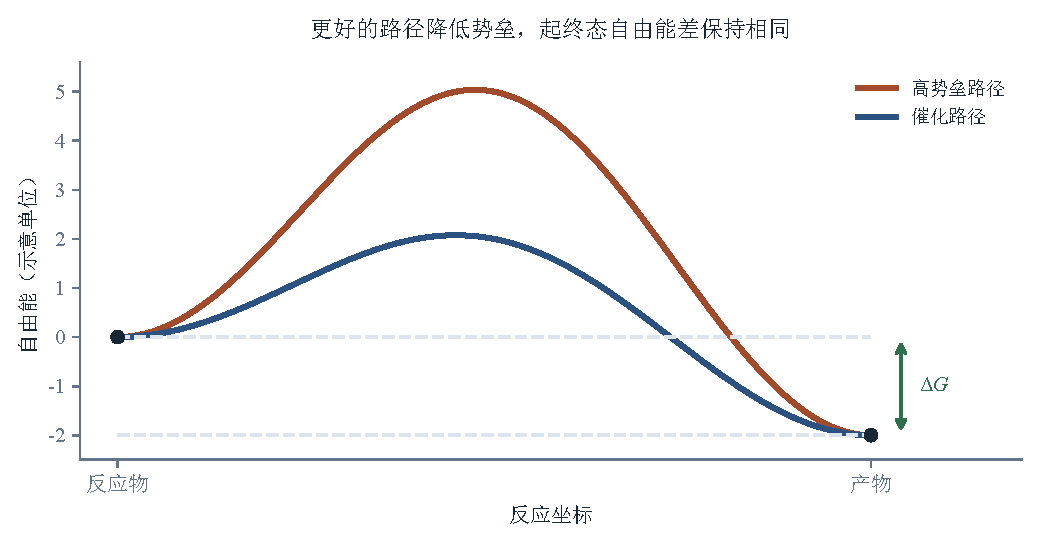
\includegraphics[width=\textwidth]{figures/activation-barrier.pdf}
\caption{催化改变路径与动力学势垒。图中的两条示意路径有相同起终态，$\Delta G$保持相同；降低活化自由能有助于加快速率，反应平衡由起终态决定。}
\label{fig:mechanism-activation-barrier}
\end{figure}
\subhead{智能在这条链上的位置}

智能可以筛选催化剂、寻找新反应路线、优化工艺窗口、调度能源并预测故障。催化会改变反应路径与速率，工艺整合也能回收热量、减少分离支出。改进应通过整个过程的能耗、良率、产能、安全与停机时间来衡量。

更麻烦的是，智能系统自身也在资源势垒之内。数据中心可以通过硬件、冷却和利用率提升显著改善能效，但“效率提高”不等于“物理基础消失”，大规模计算仍然要占用设备、土地、电力、冷却系统、技术链条和维护能力。\cite{masanet2020recalibrating}信息处理本身也不是脱离物理的幽灵，兰道尔原理至少提醒我们，信息擦除和逻辑不可逆操作存在热力学下限，尽管这一原理不能被粗暴地直接换算成所有现实计算系统的总能耗。\cite{landauer1961}

因此，判断一项技术是否真正降低现实代价，不能只看它在信息空间中生成了多少方案，而要看它是否减少了现实中的材料消耗、能量损耗、工艺步骤、维护负担和长期不可逆后果。如果一个方案只是把消耗转移到更深的技术链条、能源系统、算力后台或维护结构中，它没有突破资源势垒，只是改变了资源势垒的位置。真正可靠的技术进步，不是用比特逃离原子，而是在原子的硬约束中，用更好的路径完成不可豁免的状态转移，现实改变的本质，不是让可能性出现，而是让物质在可用能推动下，进入一个可维持的新秩序。

\subsection{宏观质量堆积与重力势能库的建立}

技术系统向物质底层推进时，遇到的边界形式取决于尺度。改动的对象越大、越小、越分散，阻挡它的东西就越不是同一类东西；上一段说的那三种边界因此会在不同的尺度上轮流成为主导项，而哪一项主导，决定了这一层的成本该往哪里记。

物质重构最常见的误判，是把原子世界想象成一种可以任意缩放、任意编辑、任意循环的软件空间。宏观上，似乎只要有更好的规划，就能改写城市和基础设施；微观上，似乎只要技术继续进步，就能无限缩小、无限精密；资源上，似乎只要回收体系足够完善，物质就可以被无限循环。现实并不是这样。原子世界有尺度，尺度一变，阻力的形态就会改变：宏观尺度上，阻力表现为质量、惯性和沉没结构；微观尺度上，阻力表现为热噪声、缺陷、量子效应和散热压力；元素尺度上，阻力表现为丰度、分布、提纯和循环不可逆。物质重构不是在一个均匀平面上移动符号，而是在不同尺度中穿过不同的物理边界，可以把它压缩为一句话：\key{宏观世界太重，微观世界太吵，元素世界太散。}

\subhead{质量与惯性}

先看宏观尺度，它的第一性约束是质量。质量不是单纯的重量，而是过去做功的沉积，凡是已经被开采、运输、抬升、固定、连接和维护的东西，都不只是物体，而是材料、能量、土地、劳动、制度和时间共同凝结成的结构，建筑、道路、桥梁、地铁、电网、管网、港口和厂房，都是过去投入在现实中的物理记忆。城市尤其如此，城市不是地图上的区域，也不是经济活动的抽象容器，而是亿万吨钢筋、水泥、玻璃、沥青、铜缆、管道和设备被抬升、固定、连接之后形成的高势能系统。建筑抵抗重力，桥梁跨越空间，地铁穿透地层，电网输送功率，管网维持流动，道路组织人和物的运动，城市是固化的能量，也是凝固的历史做功。

这类堆积的规模可以用物质流来衡量。水泥、钢铁、砂石等建筑材料构成了现代社会的物质存量主体，二十世纪全球社会经济物质存量增长了二十余倍，其中建筑和基础设施占绝大部分；\cite{krausmann2017global}人类每年搬运的土石方和沉积物总量已经与全球河流的自然输沙量相当甚至更高，在部分流域，人类搬运量超过自然侵蚀量。\cite{syvitski2005impact}城市就是这些流量的最终沉淀形式，这也正是原子世界更新缓慢的原因：旧建筑不是可以删除的文件，旧道路不是可以回滚的版本，旧管网不是可以重绘的图层，它们占据空间，绑定生活，牵连产权、金融、法规、习惯和日常路线。重构一片城区，不只是生成更好的方案，而是废弃已经固化的材料和势能，再支付拆除、运输、污染、替代、施工和社会协调成本。

到这里可以回答一个合理的反驳：如果质量是主要阻力，那么单位成本更低的方案应该自动胜出，为什么实际不是这样。原因是质量约束并不只体现在造价上，它通过产权、管网接口、施工窗口、生活习惯和既有路线把替换成本分散到很长时间里，单个决策者看到的往往只是其中一小段，于是更优方案在局部账面上划算，在整体账面上不划算。质量带来的这种性质有两面：一面是可靠，另一面是难改。桥梁之所以可用，是因为它足够坚固；城市之所以难改，也是因为它足够沉重。基础设施之所以能长期服务，是因为它把物质固定在稳定结构中；基础设施之所以难以快速迭代，也是因为这种稳定结构已经嵌入现实生活，宏观世界的阻力不是偶然阻力，而是过去成功建造所留下的惯性。

所以，许多技术落地不是败给观念保守，而是败给质量堆积：一个更优的交通方案，不能自动搬走旧道路；一个更好的能源系统，不能瞬间替换电网；一个更聪明的城市算法，不能让楼宇、管网、停车场、地铁线路和土地格局同步重排。宏观尺度的重构，本质上是在已经存在的重量中改写重量。这也是为什么数字技术进入原子世界时，常常先选择覆盖，而不是重建：给旧道路加导航，给旧工厂加传感器，给旧医院加AI分诊，给旧城市加监控平台，比推倒重构底层结构便宜得多。先覆盖而不是重建，不是偶然选择，而是宏观质量惯性下的现实路径：旧世界太重，新技术只能先附着在旧世界表面。

\subhead{重力势能库}

把建筑材料抬高，会增加重力势能。对给定质量与平均抬升高度，理想净功为

\begin{equation}
W=m\,g\,h
\end{equation}

$W$为重力势能增量，$m$为质量，$g$为当地重力加速度，$h$为平均抬升高度。以$m=10^8$千克、$h=250$米计算，$W$约为$2.45\times10^{11}$焦耳。设计能够改变用料、结构与高度；给定这些量，抬升账目才固定下来。施工中的耗散、材料制造与其他能耗另计。拆除释放的势能通常会耗散，能够回收多少取决于实际装置。城市更新还受拆解、运输、基础设施、产权与持续服务约束，储存的势能只占其中一项。

年度材料流显示另一种规模。2026年出版的USGS与worldsteel资料分别汇总2025年水泥与钢铁产量，前者在40亿吨量级，后者接近20亿吨。\cite{usgs2026cement,worldsteel2026figures} 水泥不等于熟料，理论反应热不等于全流程实际能耗，核算时须分别采用对应产量与工艺。矿山、加工、运输与施工共同构成一条持续运行的物质通道，城市是这条通道长期积累的结果。

势能库建成之后，它的约束方式与流量型能源不同。木材和畜力的约束是通量，只要当年产出不够，系统就停止扩张；固化质量的约束是存量，它不限制继续堆叠，却把改变的成本抬高到必须在很长时间里摊销。一座城市的重心、管网走向、道路格局和土地权属会同时约束此后几十年的所有改造方案，新的方案只能在既定几何中寻找缝隙。宏观尺度的阻力因此有一个反直觉的性质：它并不妨碍建造，它妨碍的是重新建造。

\subsection{微观尺度缩微的量子效应与热流密度极限}

把尺度缩小，情况并没有变简单。宏观尺度上，物体越大越难搬动；微观尺度上，结构越小越难控制，而且控制的对象从位置变成了概率。缩微在物理上从来不是简单的比例缩小，尺寸每下降一个量级，起作用的物理机制就会换一批。芯片是这条路径上被走得最远的一个例子，它同时也把缩微的两类极限暴露得最清楚：一类来自量子力学，一类来自热力学。

\subhead{噪声与热}

人们常以为小意味着轻，轻意味着便宜，但越接近原子、电子和量子尺度，世界越不再像宏观物体那样稳定可控，热噪声、表面效应、缺陷概率、量子隧穿、材料涨落、测量扰动和散热密度开始变得不可忽略。微观世界的阻力不是搬不动，而是控不稳；不是质量太大，而是扰动太多。芯片是最典型的例子：比特看似轻盈，软件看似可以无限复制，但制造比特的物理底座极其沉重。要让电子在纳米尺度按人类意图稳定运动，需要高纯材料、洁净室、真空环境、精密光刻、温度控制、化学处理、缺陷检测和全球供应链。芯片越小，制造它所需的环境控制系统越大；电子路径越短，支撑它的秩序密度要求越高，微观世界不是越轻越便宜，而是越精密越依赖庞大的后台工程。

微观缩小并不是简单比例缩小。宏观加工可以容忍粗糙，微观制造必须压低杂质、振动、热扰动和缺陷：一个肉眼不可见的颗粒，可能毁掉一片复杂结构；一个微小工艺漂移，可能影响大量器件性能；一个局部热点，可能限制整个系统的功率密度。越小的结构，越依赖更大的环境控制系统，小不是无重量，而是把重量转化为秩序密度。工程史给出了这条路径的终点：晶体管尺寸在几十年里持续缩小的时候，功耗密度还能按比例下降，频率可以不断提高，这一趋势在2005年前后停止，此后时钟频率长期停留在数吉赫兹量级，芯片性能的提升越来越依靠并行和专用结构，而不是继续提高单核频率。\cite{esmaeilzadeh2011dark}随之出现的问题是暗硅：受功率密度和散热能力限制，芯片上大部分晶体管在同一时刻无法同时以最高频率工作，一部分面积必须在任意时刻保持低功耗状态。\cite{esmaeilzadeh2011dark}

这条路径并没有被完全堵死，但绕开的办法只是把约束换了位置。三维堆叠、专用加速器和先进封装确实把一部分压力从尺寸转移出去，代价是散热通道变得更长、互连更复杂、良率更敏感，原来落在晶体管上的限制改由热流密度和封装工艺承担。这就是微观尺度的悖论：产品越轻，制造条件越重；单个元件越小，系统后台越大；信息越便宜，信息底座越昂贵。先进制造并不是物质性消失，而是物质性被压入更深的工艺、设备、能源和环境控制之中。

\subhead{量子效应：隧穿与统计涨落}

量子效应进入制造流程的方式，先是隧穿，然后是统计涨落。芯片上控制电流通断的栅极靠一层极薄的绝缘层隔开沟道，这层氧化物的厚度在持续缩微中降到了1.2到1.5纳米，也就是五六个原子层的量级。在这个厚度上，电子不再被势垒完全挡住，它有确定的概率直接穿过绝缘层，形成隧穿漏电流。漏电流随厚度指数上升，一旦它超过开关本身所需的电荷，继续减薄绝缘层就不再带来收益，只能改用高介电常数材料去换回等效的厚度。这是量子力学直接进入工艺决策的一个例子：不是工艺做不到更薄，而是更薄之后器件不再按电路设计的规则工作。

统计涨落来自同一个方向。器件沟道里参与导电的掺杂原子数目随体积缩小而下降，当数目降到几十个量级时，原子个数的随机波动直接转化为器件参数（如阈值电压）的器件间差异，同一批芯片上相邻的两个晶体管可能表现出明显不同的特性。这条约束无法靠提高加工精度消除，因为它的来源是掺杂原子的离散性和泊松统计，而不是机器的定位误差。类似的涨落还出现在制造工艺的上游：光刻使用的极紫外光波长13.5纳米，单个光子能量约92电子伏特，是深紫外光子的十多倍，在相同曝光剂量下到达晶圆的光子数目只有后者的十几分之一。光子到达服从泊松分布，落入一个小面积区域的光子数目的相对涨落随数目的平方根下降，特征尺寸缩小、区域面积减小时，光子数急剧下降，相对涨落急剧上升，本该平直的线条边缘因此变成锯齿状。要让涨落减半，曝光剂量必须提高到四倍。把这条统计关系写成式子是直接的，

\begin{equation}
\sigma_{N}=\sqrt{N},
\qquad
\frac{\sigma_{N}}{N}=\frac{1}{\sqrt{N}}
\end{equation}

式中 $N$ 为落入某一小面积区域的光子数，无量纲计数，也可以换成其他相互独立、随机到达的事件的计数；$\sigma_{N}$ 为它的标准差，量纲与 $N$ 相同；$\sigma_{N}/N$ 为相对涨落，无量纲。第二式说明相对涨落随计数按平方根下降：要让涨落减半，$N$ 必须增大到四倍。这正是特征尺寸缩小之后曝光剂量必须急剧上升的原因，也是极紫外光刻必须以二十千瓦级的激光输入换取二百五十瓦级曝光功率的原因之一。它的适用边界是：平方根关系只对相互独立、平均到达率稳定的泊松过程成立；若光源强度本身漂移，或者相邻区域的曝光存在关联，实际涨落会偏离 $1/\sqrt{N}$，所需剂量必须实测，不能按这个式子外推。为了在硅片上得到一条确定的线，上游必须投入远高于此的能量，量产极紫外光刻机的能量转换效率因此长期低于2\%：输入二十千瓦级的激光功率，最终可用于曝光的极紫外光只有二百五十瓦量级，其余都变成废热、碎片和动能冲击。\cite{debisschop2018stochastic}这里出现的不是工艺粗糙，而是确定性本身的代价：在原子尺度的加工区域里，每一次曝光只涉及有限个光子，统计规律就必然在成品上留下痕迹。

\subhead{热流密度墙}

热也是微观边界的一部分，计算、通信、制造和控制都要耗能，耗能就要散热，微观结构可以提高密度，却不能取消热流。器件越密集，功率越集中，散热越成为限制，很多时候限制系统继续前进的不是逻辑设计，而是热如何排出、噪声如何压低、缺陷如何控制。散热能力由材料导热、界面热阻和冷却介质共同决定，通道越窄，单位面积能带走的热流越难提高，风冷能够稳定处理的热流密度被限制在每平方厘米百瓦量级，超过这个水平就必须引入液冷、相变或更复杂的封装结构。把这个约束写成式子是直接的，

\begin{equation}
q=\frac{P}{A}=-k\,\frac{\Delta T}{L}
\end{equation}

$q$ 为热流密度，单位瓦每平方米，正文中风冷的上限用每平方厘米百瓦表示，合 $10^{6}$ 瓦每平方米量级；$P$ 为需要排出的功率，单位瓦；$A$ 为散热面积，单位平方米；$k$ 为材料的导热系数，单位瓦每米开尔文；$\Delta T$ 为沿散热路径的温差，单位开尔文；$L$ 为散热路径长度，单位米；负号表示热流方向沿着温度下降的方向。等号右边的三个量各有各的上限：$\Delta T$ 受器件工作温度与外部环境的夹逼，$k$ 由材料决定，$L$ 在三维堆叠中只会变长。通道变窄之后单位面积能带走的热流更难提高，对应的就是 $L$ 增大而 $q$ 下降；而功率密度的上升速度快于这几项的改善速度，差额就落在频率停滞和暗硅上。它的适用边界是：这是稳态、单一导热机制下的线性关系，相变、对流与辐射不遵从这一形式；真实封装中的界面热阻往往比材料本身更限制 $q$，所以这个式子给出的是量级判断，不是封装设计公式。功率密度的上升速度却比散热能力的改善快得多，两者之间的差额就表现为频率停滞和暗硅。

把这条约束放大到设施尺度，形状是一样的。数据中心把计算集中到少数几个地点，散热、供电和土地随之集中，冷却系统的规模成为选址与扩容的前置条件，能效改善可以把单位算力的能耗压下去，却压不掉热流本身。信息系统越往微观深入，它的上游越依赖一套宏大的宏观工程，而宏观工程的散热能力有上限。芯片越先进，这个上限越紧。\key{信息系统的尽头，仍然是热力学系统。}

\subsection{宇宙元素丰度与物质循环的热力学约束}

如果说宏观尺度的阻力来自质量，微观尺度的阻力来自噪声，那么元素尺度的阻力则来自丰度和分布。元素的多寡不由需求决定，而由核合成和行星分异决定，技术可以改变提取效率，不能改变分布本身。这一层的约束方式与前两层不同：质量可以被搬动，噪声可以被隔离，元素的分布只能被接受，然后靠更大的处理量、更长的流程和更高的能耗去迁就它。也正因为如此，元素层面的约束最难被工程手段绕过，最容易在供应紧张时以价格和工期的方式显形。

\subhead{丰度与熵税}

元素不是均匀摆放在地球表面的材料库，它们来自宇宙核合成、行星形成、地质分异、矿化过程和漫长地球历史，碳、氧、硅、铁、铝、铜、锂、镍、钴、稀土、铂族元素，并不是以人类需要的方式均匀存在。宇宙中有某种元素，不等于地球上有足够可用储量；地壳中存在，不等于形成了可开采矿床；产品中含有，不等于能够低成本回收。地壳的元素分布本身就是高度不均匀的：氧和硅两种元素合计约占地壳质量的四分之三，铝和铁各占百分之几，而铜的平均丰度在百万分之六十量级，锂在百万分之二十量级，稀土元素合计在百万分之一百至两百量级，铂族元素则低到十亿分之一量级。\cite{rudnick2003composition}这些比例由恒星核合成和行星分异过程决定，不受需求影响，技术可以提高提取效率，可以寻找替代材料，但不能让某种元素在世界上变得更常见。

由此推出的判断与上两节一致：资源问题的关键，不是“有没有某种元素”，而是它是否以足够浓度、足够规模、足够稳定、足够低成本的方式处在可用状态中。低品位矿不是没有资源，而是资源过于分散，需要更高能耗和更大处理量才能利用；稀有元素也不是完全不存在，而是浓度低、分布不均、提取复杂、伴生关系强，并常常受到地理和产业链约束。这使得物质循环不可能成为热力学意义上的免费过程：回收不是把物质重新拿回来这么简单，而是把已经分散、混合、污染、降级和嵌入复杂产品中的物质重新带回可用状态，它需要收集、拆解、分离、提纯、再加工和质量控制。循环可以降低原生开采压力，但循环本身也消耗能量、设备和时间。

回收需要收集、拆解、分离与再加工。这些步骤消耗资源，也可能比原生开采与冶炼节约大量能量。要比较的是同一材料、同等品质与同一边界下的全流程：产品中的浓度、污染、拆解设计与运输距离，都可能改变结果。循环的价值来自实际减少的新开采、能耗与废弃负担。

这可以称为元素层面的熵税。只要物质被分散、混合、污染和降级，重新集中它、分离它、提纯它，就必须付出新的能量、设备和时间，技术可以降低这笔税，不能让这笔税归零。分散的物质不会免费回到高浓度状态，混合的材料不会免费拆分成纯净组分，循环本身不是逃离熵增，而是在熵增之后重新支付秩序恢复成本。因此，元素尺度提醒我们：物质世界不是无限可调的库存，而是由丰度、位置、浓度、化学状态和循环损耗共同构成的约束场。技术可以提高提取效率，改善替代材料，优化回收流程，但不能让宇宙元素丰度重新洗牌，不能让分散物质无成本集中，不能让混合物无能耗分离，不能让循环没有熵税。

\subhead{元素从哪里来}

元素供给带着宇宙与地质历史。大爆炸核合成主要形成氢、氦，恒星内部反应与后续演化产生许多更重元素。铁峰附近之后的合成包含恒星中的慢中子俘获，以及中子星并合等环境中的快中子俘获等路线。\cite{steigman2007primordial,kobayashi2020origin} 地球上的可用矿床还要经过行星分异、岩浆、热液与风化富集。工程面对的是这些过程留下的浓度、位置与化学状态。

行星形成和地质分异又对这份清单做了一次重新分配。地球形成时的分异过程把亲铁元素带进地核，把亲石元素留在幔壳，地壳中的可用矿床再经过数十亿年的岩浆活动、热液迁移和风化富集才形成。这意味着两件事：一是元素的绝对数量由宇宙和行星过程给定，二是这些元素在地表是否集中成矿，取决于后来的地质历史。人类可以开采的部分，只是这两个过程叠加之后留下的少数异常富集区。技术能改变的是对富集区的要求，品位可以从百分之几降到百万分之几，但每降一个量级，处理量、能耗和废物就要上一个台阶，熵税的斜率不会变。把处理量与品位之间的关系写成式子是直接的，

\begin{equation}
M=\frac{m}{\theta}
\end{equation}

这里 $M$ 为获取给定目标元素所必须处理的原矿质量，单位千克或吨；$m$ 为其中目标元素的质量，单位与 $M$ 相同；$\theta$ 为品位，即目标元素在原矿中所占的质量分数，无量纲，工业上常用百分比或百万分之一表示。反比关系给出那句判断的全部内容：品位每下降一个数量级，为了得到同样多的目标元素，需要开采、破碎、浸出和处理的物料就上升一个数量级，能耗、试剂与废物同步上升，熵税的斜率就是这条反比关系。它的边界有两处：一是这里只算物料量，不含提取率，实际回采与选冶的回收率都小于 1，真实处理量比 $M$ 更大；二是当矿物相复杂、多元素伴生时，能耗随品位下降常常比 $1/\theta$ 更快，因为磨矿要更细、分离步骤要更多。因此在真实矿山上，这个式子是乐观下限，不是预测。

\subhead{三种尺度的共同含义}

把三个尺度放在一起，它们共同说明：原子世界不能像软件一样任意重写。宏观上，质量留下惯性；微观上，噪声限制控制；元素层面，丰度和分布约束可用性。每一层都有自己的边界，每一层都要求不同形式的代价，物质重构不是一场在抽象空间中的优化，而是在不同尺度上制造和维持结构的过程。这也意味着，物质重构的难点不只是“能不能设计出来”：设计发生在表示空间，尺度边界发生在现实空间，一个更好的城市规划必须穿过宏观质量惯性，一个更先进的芯片设计必须穿过微观制造极限，一个更理想的能源方案必须穿过元素丰度、矿产分布和循环热力学。方案可以轻盈，尺度不会轻盈。

三个尺度上的边界形态不同，指向的却是同一件事：物质重构必须在尺度中发生。它可以优化城市更新路径，减少拆除浪费；可以改进芯片设计和制造控制，降低缺陷率；可以寻找替代材料，提高资源循环效率；可以在复杂供应链中减少无效消耗。这些都做得到，但穿越尺度边界时的浪费减少了，尺度边界本身不会消失。尺度边界的意义，不是说技术无法进步，而是提醒我们技术进步必须在尺度中发生，真正成熟的物质重构，不是幻想把世界压成可编辑的平面，而是理解不同尺度上的阻力形态：在宏观上尊重惯性，在微观上管理噪声，在元素层面承认可用性的稀缺。原子世界不是慢版软件，它有重量，有热，有噪声，有丰度，有历史，它的更新缓慢，不只是因为人类组织低效，而是因为物质本身在不同尺度上保留了自身的抵抗。\key{世界可以被改变，但不能被任意改写。}

以上三种边界都是关于空间和物质的：多大的质量被固定，多小的结构被维持，多稀的元素被集中。它们回答的是物质在尺度上如何抵抗重构，没有回答时间被压缩时会发生什么。而时间压缩不会改变这些边界，只会把它们重新组织一遍：同样多的质量、同样多的热、同样多的缺陷，被要求在同一条更短的窗口里通过系统。通量一旦成为主要约束，尺度上的三重边界就会以另一种形式重新出现。

% <<<<<<<<<< parts/book-ch02a.tex <<<<<<<<<<


% >>>>>>>>>> parts/book-ch02b.tex >>>>>>>>>>
\section{时间的刚性：不可压缩的过程}

\subsection{物理过程的非零时长属性}

资源的账本回答的是物质从哪里来，还没有回答它要多久才能就位。加速不减少任何载荷，它只改变载荷通过系统的速率。同一份材料、同一份能量、同一份热和同一份误差，被要求在同一条更短的窗口里通过系统。当时间成为约束，空间的三种边界不再分头出现，而是转换成同一个量：单位时间内的负荷。

把时间当作可以压缩的资源，是智能时代最普遍的假设。这个假设在信息侧确实成立：等待可以被消除，重试可以被并行，搜索可以被剪枝，一个环节的延迟不会自动传递给下一个环节。但在物质侧，同一个状态转移，占用的材料、注入的能量、产生的热、积累的损伤和维护需求都要在更短的窗口里被处理完。

AI时代最容易产生的错觉，是把速度等同于效率。模型可以快速生成答案，系统可以快速响应信号，平台可以快速分发内容，组织可以快速获得指标，于是人们很自然地认为越快越好，只要把过程压缩，把等待消除，把反馈拉高频，现实系统就会变得更有效率。但时间不是一个可以任意删除的空白。在现实系统中，一个状态转移总要穿过材料、能量、设备、身体、组织和环境，把同一个状态转移压进更短时间，并不只是“少花时间”，而是提高单位时间内穿过系统的通量。时间越短，系统必须在同一窗口内处理更多能量、更多物质、更多热、更多误差和更多风险，加速的本质，不是速度本身，而是通量密度上升。

反应、扩散、养护、生长与服役各有时间尺度。计算可以帮助改变配方、设备、温度、顺序与并行方式，从而缩短其中一些过程；某些长期结果仍须通过足够暴露才能确认。设计速度、制造速度与获得证据的速度，需要分别记录。

\subhead{通量密度}

通量密度可以用一个简单的量描述：
\begin{equation}
J=\frac{\Delta X}{A\,\Delta t},
\label{eq:flux}
\end{equation}
其中$J$为通量密度，表示单位截面上单位时间内通过的载荷量；$\Delta X$为这次状态转移需要穿过的载荷总量，按对象不同可以是能量、物质、热量、误差或需要承接的后果，量纲随对象而定；$A$为系统的通量截面，即系统在单位时间内能够承受该载荷的有效截面积；$\Delta t$为完成这次转移所允许的时间窗口，单位秒。这个关系成立的前提是系统处在同一工作区间内，即截面$A$不随负荷提高而自动扩大。它给出的是一个比例判断：在$\Delta X$和$A$不变时，把$\Delta t$缩小到原来的十分之一，$J$就上升到十倍，而系统能否承受十倍的通量密度，与$J$的升高无关，只由$A$决定。同样一件事，用十天完成和用一天完成，系统面对的不是同一个过程：能量要更集中地注入，废热要更快排出，设备要承受更高负荷，人员要减少修正时间，错误会更快扩散，失败也更少有机会被早期截断。时间被压缩之后，并不会消失，而会以功率、热流、应力、检测压力和修复压力的形式重新出现。

因此，加速能否成立，不取决于目标时间能否写进计划，而取决于系统是否有足够的通量截面。所谓通量截面，是系统承受单位时间流量的能力，它包括供能截面、散热截面、承载截面、检测截面、修复截面和责任截面。供能截面不足，过程无法驱动；散热截面不足，系统会升温；承载截面不足，结构会疲劳；检测截面不足，缺陷会穿过系统；修复截面不足，小错误会被复制成大故障；责任截面不足，快速行动后的后果无人承接。这比“速度有代价”更根本，问题不是快本身，而是快把原本分散在时间里的负荷压缩到了更窄的窗口。时间原本承担了一部分缓冲功能，它让热有时间扩散，让材料有时间释放应力，让人员有时间检查，让组织有时间协调，让错误有时间显影。加速切掉这些缓冲，就必须用更强的结构、更高的冗余、更快的检测和更大的维护能力来替代。

这里有一种常见的辩解：既然缓冲可以用技术替代，加速的极限就只是投入多少的问题，而不是原理问题。这个说法在单个环节上常常成立，放到系统上却不成立，因为六类截面并不彼此独立。加厚结构能提高承载截面，同时增加质量和热容；提高刷新率能扩大检测截面，同时增加能耗和误报；增加冗余能提高修复截面，同时提高协调成本；把决策交给自动过程能加快责任截面的通过速度，同时削弱责任归属。加宽一个截面往往压缩另一个截面，所以加速不是一次可以买断的投资，而是必须持续维持的结构代价。这也是为什么加速不是线性的：把十天压缩到五天，可能只是减少等待、优化排程、削掉返工；把五天压缩到一天，可能就需要更多设备、更强并行、更高库存、更密集检查；把一天压缩到一小时，可能已经触及散热、可靠性、安全边界和责任承载。越接近系统极限，时间每缩短一分，后台强度往往不止增加一分，边际加速阻抗会迅速上升。

混凝土的强度随水化发展，28天是常用检验龄期，实际养护要求则随材料和工程条件确定。大体积浇筑还要控制水化热与温差，施工分层、冷却和保温都在改变可行的节奏。锂离子电池的高倍率充电则可能受到传输、嵌入和析锂等机制限制。加速这些过程，需要改变材料、温度、结构或操作方式，再检验相应的成本与寿命。

通信和计算提供了另外两个界。光纤中的光速只有真空中的约三分之二，跨洋通信的单程延迟因此在几十毫秒的量级；增加波长、提高功率、加密中继都能扩大带宽，却不能让信号提前到达，带宽是可以扩的截面，延迟不是。单核时钟频率在 2005 年前后停在了数 GHz 量级，继续提高频率会让功耗密度超过散热能力，算力的增长因此转向多核并行。并行能够摊销的只是彼此独立的步子，不能减少一条依赖链上的步数，这条界线在后面的讨论中还要反复用到。

\subsection{功率与时间的互斥方程}

通量密度上升还只是一个描述，没有说明负荷落到哪些量上。把同一件事压进更短的时间窗口，时间挤出来的负荷会依次出现在几个可以分别考察的地方，它们的次序不是随意的，前一个量决定了后一个量的规模。
\begin{figure}[ht]
\centering
% >>>>>>>>>> figs/fig-power-time.tex >>>>>>>>>>
% 图 2-3  功率与时间的互斥，以及压不动的功率天花板
% 双对数坐标：1 个数量级 = 横向 1.25 cm、纵向 0.72 cm。
% 固定能量需求 E 对应等能线 P·t = E；沿同一条线只能「用功率换时间」，
% 整条线下移一格（能量需求降一个数量级）才叫效率改善，斜率不变。
% 水平虚线是材料强度、传热密度、电网容量共同设的功率天花板；
% 它与等能线的交点给出最短时间 t_min——这才是时间压不下去的原因。
\begin{tikzpicture}[x=1cm, y=1cm, font=\small,
  ax/.style={-{Stealth[length=2.0mm]}, ink, line width=0.6pt},
  tk/.style={font=\scriptsize, text=slate, anchor=north},
  yk/.style={font=\scriptsize, text=slate, anchor=east}
]
% 上缘原先 1.30，纵轴的 $E$ 标注与「：现行路线的能量需求」距页边只剩约 2pt。放宽到 1.55。
\useasboundingbox (-1.35,1.55) rectangle (12.75,-6.30);

\def\aX{1.05} \def\aY{-4.90} \def\dx{1.25} \def\dy{0.72} \def\aR{11.15}
\pgfmathsetmacro\yTop{\aY+\dy*9.2}

\draw[ax] (\aX,\aY) -- (\aR,\aY) node[anchor=west, font=\scriptsize, text=ink] {时间 $t$ (s)};
\draw[ax] (\aX,\aY) -- (\aX,\yTop)
      node[anchor=south, font=\scriptsize, text=ink, yshift=1pt] {功率 $P$ (W)};

\foreach \e in {0,...,7} {
  \pgfmathsetmacro\xx{\aX+\dx*\e}
  \draw[slate!55, line width=0.4pt] (\xx,\aY) -- (\xx,\aY-0.07);
  \node[tk] at (\xx,\aY-0.10) {$10^{\e}$};
}
\foreach \e in {0,2,4,6,8} {
  \pgfmathsetmacro\yy{\aY+\dy*\e}
  \draw[slate!55, line width=0.4pt] (\aX,\yy) -- ({\aX-0.07},\yy);
  \node[yk] at ({\aX-0.09},\yy) {$10^{\e}$};
}

% ---------- 守恒律禁区：最下面那条等能线之下（先铺底，线压其上）----------
\begin{scope}
\clip (\aX,\aY) rectangle (\aR,\yTop);
\fill[slate!10] ({\aX+\dx*1},{\aY+\dy*7}) -- ({\aX+\dx*7},{\aY+\dy*1})
      -- ({\aR},{\aY+\dy*1}) -- ({\aR},\aY) -- ({\aX+\dx*1},\aY) -- cycle;
\end{scope}

% ---------- 两条平行的等能线 ----------
% E=10^9：f = 9 − e；E=10^8：f = 8 − e。两线相距恰好一个数量级。
\draw[terra!90, line width=1.7pt] ({\aX+\dx*1},{\aY+\dy*8}) -- ({\aX+\dx*7},{\aY+\dy*2});
\draw[forest!85, line width=1.5pt, dashed] ({\aX+\dx*1},{\aY+\dy*7}) -- ({\aX+\dx*7},{\aY+\dy*1});
\node[font=\scriptsize, text=terra!90, anchor=south west] at ({\aX+\dx*1.02},{\aY+\dy*8.10})
      {$E=10^{9}$ J：现行路线的能量需求};
\node[font=\scriptsize, text=forest!85, anchor=south east] at ({\aX+\dx*7.0},{\aY+\dy*1.12})
      {$E=10^{8}$ J：效率改善后};
\draw[ink!55, line width=0.5pt, {Stealth[length=1.4mm]}-{Stealth[length=1.4mm]}]
      ({\aX+\dx*6.30},{\aY+\dy*2.70}) -- ({\aX+\dx*6.30},{\aY+\dy*1.70});
\node[font=\scriptsize, text=ink, anchor=west] at ({\aX+\dx*6.42},{\aY+\dy*2.20})
      {一格};

% ---------- 功率天花板：说明块放在线右侧上方空白，短箭头指回交点 ----------
\def\ceil{\aY+\dy*6.6}
\draw[rust!90, line width=1.1pt, densely dashed] ({\aX+0.05},\ceil) -- ({\aR-0.05},\ceil);
\node[font=\scriptsize, text=rust!90, anchor=south west, align=left]
      at ({\aX+\dx*3.30},{\aY+\dy*6.78})
      {功率天花板：材料强度、传热密度、电网容量\\[1pt]天花板以上不可达，任何工艺都进不去};
\draw[rust!75, line width=0.6pt, -{Stealth[length=1.6mm]}]
      ({\aX+\dx*3.18},{\aY+\dy*6.62}) -- ({\aX+\dx*2.52},{\aY+\dy*6.62});

% ---------- 交点给出最短时间 ----------
\pgfmathsetmacro\xmin{\aX+\dx*2.4}
\draw[slate!65, line width=0.5pt, dotted] (\xmin,\aY) -- (\xmin,\ceil);
\draw[ink, line width=1.6pt] (\xmin-0.12,\aY) -- (\xmin+0.12,\aY);
\node[font=\scriptsize, text=ink, anchor=north] at (\xmin,\aY-0.10) {$t_{\min}$};

% ---------- 沿线设备 ----------
\foreach \ex/\ey in {1.4/7.6, 2.4/6.6, 4.0/5.0, 6.0/3.0} {
  \node[circle, fill=ink, inner sep=1.4pt] at ({\aX+\dx*\ex},{\aY+\dy*\ey}) {};
}

% ---------- 禁区注记 ----------
\node[font=\scriptsize\heiti, text=slate, anchor=north east]
      at ({\aR-0.15},{\aY+\dy*0.58})
      {等能线之下：能量不够，任何工艺都做不到};
\end{tikzpicture}

% <<<<<<<<<< figs/fig-power-time.tex <<<<<<<<<<

\caption{功率与时间的互斥。固定能量需求对应等能线 $P\cdot t=E$，沿同一条线只能以功率换时间；整条线平移一格才叫效率改善，斜率不变。水平虚线是若干物理上限共同设定的功率天花板（其来源已在图内标出），它与等能线的交点给出最短时间 $t_{\min}$，这才是时间压不下去的原因。}
\label{fig:power-time}
\end{figure}


\subhead{四层阻抗}

第一层阻抗是功率。现实改变需要做功，搬动物体、驱动设备、压缩流程、提高产量、加快运输，本质上都要在单位时间内完成更多状态转移。能量除以时间就是功率：
\begin{equation}
P=\frac{\Delta W}{\Delta t},\qquad \Delta W\ \text{固定时}\ P\propto\frac{1}{t},
\label{eq:power}
\end{equation}
其中，$P$为功率，单位瓦特，即焦耳每秒；$\Delta W$为完成这次状态转移所需的功，单位焦耳；$\Delta t$为所用时间，单位秒。它成立的条件是功总量不因加快而减少，也就是路径、工艺和材料都没有变化，只是把同一件事做得更快；如果加快同时改变了工艺并降低了$\Delta W$，这个反比关系就要重新计算。由这个关系可以直接读出结论：时间减半意味着功率加倍，时间压缩一个数量级意味着功率上升一个数量级。相同能量消耗被压缩到更短时间，就要求更高功率输入，系统如果没有对应的供能、传输和控制能力，加速就会表现为过载。工业生产最容易看见这一点，产线提速不只是机器转得更快，还意味着供料、加工、检测、包装、物流和维护都要同步承受更高节奏，任何一个环节的功率截面不足，都会成为瓶颈，一个环节被强行加速，另一个环节就会堆积，速度不是在单点上发生的，而是在整条链上结算。

电力系统把这条反比关系写进了设备选型。要把功率的调整做得更快，靠的不是把同一台机组开得更猛，而是换成爬坡能力不同的设备：燃煤机组的出力调整通常在每分钟百分之几额定容量的量级，燃气机组明显更快，电池储能的响应落在毫秒到秒的量级，而它们的单位容量成本依次上升。一个电网能够承受的风光波动幅度，最终由这套设备的爬坡能力决定。同样的道理出现在制造与运输上，把交付周期从六周压到一周，通常不是让同一批设备连轴转，而是把一部分零件改成空运、把一部分工序改成并行、把一部分库存前置，省下的时间用更高的单位成本买回来。时间与功率之间的这条交换关系是连续的，压缩越到后面，需要的功率裕度越不成比例。

功率之外，第二层阻抗是热。任何真实过程都有损耗，计算有热，机械运动有摩擦，电力传输有损耗，化学反应有副产物，生产过程有废料，速度越高，单位时间内排出的废热越多。散热不是附属问题，而是加速的核心边界之一，很多系统不是不能更快计算、更快传输、更快制造，而是不能把热、损耗和副产物以同样速度排出去。数据中心、芯片、发动机、电池、工厂和城市交通都受这一点限制：能量可以更快注入，但废热也必须更快离开，输入通量提高，而排出通量不足，系统就会升温、降频、老化或失效。热告诉我们，加速不是只看能量能不能进来，还要看无用能量能不能出去。

功率和热之外，第三层阻抗是应力。物理对象不是理想符号，材料承受力，结构承受振动，设备承受磨损，连接件承受冲击，供应链承受波动，一个系统被更快推动时，内部薄弱点会更快暴露。机器加速会增加摩擦和疲劳，施工加速会增加质量控制压力，物流加速会减少缓冲空间，组织加速会减少沟通和修复时间。应力的危险在于，它往往不立即表现为失败，而是以微损伤形式累积，疲劳、磨损、松动、裂纹、质量波动，不一定来自一次大冲击，而来自高频负荷下的长期运行，加速让系统更快接近极限，也更快积累损伤。

还剩下最容易被忽略的一层，第四层阻抗是检测与修复。越快的系统，越需要更快发现错误：慢系统中，一个错误可能有时间暴露、定位、隔离和修复；快系统中，一个小错误可能在被发现前已经复制、扩散和放大。产线速度越快，检测窗口越短；金融交易越快，错误订单传播越快；内容生成越快，审核压力越集中；科研候选越多，验证瓶颈越重。检测和修复之所以是独立的截面，是因为它们的成本不随速度线性下降：把检测频率提高一倍，往往意味着设备、人员、标准和组织流程都要同步加密，而修复能力受制于现实中的定位时间和返工周期。

四层相加之后，得到一个与直觉相反的结论：快不一定是效率。效率是以较低总代价完成有效状态转移，速度只是单位时间内完成状态转移的程度，一个系统可以很快，但能耗高、热负荷大、损耗大、错误扩散快、维护困难；也可以较慢，但稳定、低耗、可修复。真正的问题不是能不能更快，而是更快之后，系统总账是否下降。

\subhead{速度与效率}

加速试验是工程上把时间换掉的正式做法，它的边界说明了这种交换能走多远。材料与器件的寿命评估普遍采用提高温度的办法加快反应速率，再按阿伦尼乌斯关系外推常温下的使用寿命，一项原本要跑几年的试验因此可以在几个月内完成。这类方法有一个硬条件：外推必须落在同一个失效机理之内，温度高到一定程度就会出现新的反应路径、新的应力状态或新的失效模式，此时外推出来的寿命不再是原来那个过程的寿命，而是另一个过程的寿命。试验的时间被压缩了，被试验的过程并没有被压缩，两者只在机理不变的区间里等价。这一类条件在加速的每一个应用场景里都会重演，凡是把时间参数直接调小的做法，都要先证明调小之后走的还是同一条路径。

混凝土的养护给出了同一条关系的正面用法。自然养护下强度按 28 天龄期发展，若把构件放进蒸压釜，在高压饱和蒸汽中养护十几个小时，就能达到接近自然养护 28 天的强度，预制管桩和高强构件走的正是这条路。省下的二十多天不是凭空消失的，它变成了蒸压釜、锅炉、耐压模具和持续供汽的能耗，并且只适用于能在密闭容器中处理的构件尺寸。同一份混凝土，用时间还是用能量把强度换出来，取决于现场更缺哪一个。

AI在这里尤其容易制造错觉。AI极大降低了搜索、表达、生成和初步筛选的时间，这种速度真实存在，也很有价值，它可以减少无效等待，减少盲目试错，缩小候选范围，提高早期判断效率。但当 AI 输出进入现实，它面对的不是同样可压缩的信息空间，而是材料、设备、身体、工艺、实验、组织和责任，前端生成越快，后端执行、验证和维护越可能成为通量瓶颈。把一万个候选筛到一百个可以很快，但把一百个候选变成可靠结论，需要实验、测试、重复、环境暴露和长期反馈，生成方案可以高频，现实验证不能无限高频，前端越快，后端越需要足够的验证截面，否则速度只是把压力从生成端转移到验证端。

后端自动化可以扩大并行度、减少等待，也可以通过改进路线减少步骤。剩下的限制要具体说明：哪些步骤确实必须依次完成，每步在当前条件下至少需要多久，哪些后果只有经过暴露才可观察。只有在这些条件固定时，链条才有相应的历时下限。

把加速的账本摊开看，收益与代价并不落在同一本账上。一个车间把节拍从 60 秒压到 45 秒，产出在纸面上提高了三分之一，但上料、换型、检测、包装和物流必须按新节拍重排，任何一环跟不上，多出来的半成品就会堆在工序之间，占用场地、资金和后续的返工时间。设备那一侧的账更直白：提高转速意味着更高的磨损速率和更短的检修间隔，装置利用率上升的部分，要从停机检修的时间里扣回来。速度在一个环节被兑现，在另一个环节被没收，加速不是把成本消灭，而是把成本从时间账挪到设备账和维护账上。

所以，加速不是一条单向通往效率的道路。真正有效的加速，是减少无效等待、减少返工、减少无意义摩擦，让系统以更低总代价完成同样状态转移；无效加速，则只是提高通量密度，把功率、热、应力、错误和维护压到后台。成熟系统不应盲目追求最短时间，而应寻找可承受速度区间，这个区间由供能、散热、承载、检测、修复和责任共同决定：低于这个区间，系统浪费时间；高于这个区间，系统消耗结构。真正的效率，不是把时间压到最短，而是在通量截面可以承受的范围内完成状态转移。加速的阻抗，就是时间压缩后的通量账本。时间不能被简单删除，它要么被浪费，要么被用于缓冲、散热、检测、修复和显影，AI可以帮助我们减少浪费的时间，但不能免费取消承载过程所需的时间，信息可以先到，现实还必须穿过通量截面。物理世界不是拒绝速度，它只是要求速度被系统承受。

以上讨论的都是同一种加速：把一个过程压进更短的时间窗口。还有另一种加速没有被触及，它不是压缩某个过程的持续时间，而是提高对同一个系统施加更新的频率。这两件事受不同的条件限制：前者取决于通量截面是否够大，后者取决于系统完成一次完整更新需要多久。如果一个输入的间隔短于系统吸收它的时间，系统就不是在加速，而是在被打断。

\subsection{计算不可约性：物理演化的步骤刚性}

时间刚性不只是过程不能任意压缩。它还有另一种更隐蔽的形式：现实系统不能被任意频率更新。AI很容易制造一种错觉，只要模型能够更快生成、预测和调度，现实系统也应当随之更快变化：模型可以每秒输出新判断，平台可以实时刷新数据，传感器可以连续采集信号，组织可以随时更新指标，算法可以不断重算方案，于是速度被误认为智能本身，实时被误认为效率本身。但现实系统不是屏幕，不是任何输入一到就完成状态改变，一个真实系统接受变化之后，还要经历传递、执行、反馈、修正和重新稳定，只有这些过程完成，系统才真正完成了一次更新。这就是时间的带宽。

\subhead{带宽与时间尺度}

对象的响应带宽说明输入变化有多少能够在输出中体现。材料、执行器、采购与组织各有动态过程，高频信号可能被衰减，也可能通过控制结构引发不同响应。新输入早于上一轮完成，并不自动构成失稳；需要检查输入、状态和闭环如何叠加。
\begin{equation}
\frac{\mathrm{d}x}{\mathrm{d}t}=\frac{u-x}{\tau},
\label{eq:relaxation}
\end{equation}
$x$和$u$采用相同状态单位，$\tau>0$为时间常数。输入固定时，偏差按指数衰减，一个时间常数后约剩37\%。输入持续变化时，系统表现为稳定的一阶低通，响应有幅值衰减与相位滞后。闭环振荡需要加入控制器、延迟等结构后另作分析。
\begin{equation}
f_c=\frac{1}{2\pi\tau},
\label{eq:cutoff}
\end{equation}
$f_c$为一阶系统的截止频率，单位为赫兹。正弦输入频率为$f$时，稳态幅值比为$[1+(2\pi f\tau)^2]^{-1/2}$；$f=f_c$时降到低频值的$1/\sqrt2$。高频响应因此受到衰减，但这个方程本身仍是稳定的一阶跟随系统。需要更多跟随带宽时，要改变对象或控制结构。

采样频率与对象跟随输入的能力是两个设计问题。较快采样可以提供更多状态信息，控制器还需结合延迟、噪声、增益和执行器限制来选择更新方式。一阶低通系统对高频输入的响应幅度减小；闭环是否振荡，则要检查控制器与对象共同形成的环路。采样快本身既不保证稳定，也不必然引起失稳。

部分过程可以通过更快的执行器、较短的协调链和更高的传感带宽缩短响应时间；另一些过程要改变材料或结构，才能改变其时间尺度。保护动作还要区分测量、判断与执行：快速测量配合滤波和阈值，可以同时保持响应与抗扰。免疫调节、断路保护和质量检查各有机制，所需节奏须按被识别的信号与错误后果设计。

因此，现实不是低速系统，而是多时间尺度系统。越接近接触、保护、平衡、故障隔离和瞬时安全，系统越需要快速反应；越接近目标、意义、制度、信任和长期结构，系统越需要保持稳定。中间还有计划、调度、库存、维护、协调和资源配置，它们既不能太慢，也不能被高频信号直接驱动。成熟系统不是让一个中心智能以同一种频率控制全部，而是在不同层级之间分配更新时间。

电力系统的分层是这一原则的成熟形态。故障发生后的最初几十毫秒由继电保护处理，它只做一件事：把故障设备从网络中切除，动作以毫秒计；随后的秒级到分钟级由安全稳定控制与调度处理，调整出力、切负荷、隔离区域，允许的时间尺度长得多；再往上是日前与中长期的市场、检修和规划，周期以天、月、年计。每一层的权限、动作速度和判断依据都不相同，越靠近物理极限的层越不允许人参与，越靠近目标的层越不允许自动接管。这套分层不是保守的产物，而是反复事故之后被写进导则的结构，其存在的理由正是任何单一时间尺度都无法同时应付故障和规划。

具身智能最能说明这一点。机器人不能把大模型直接接到每个电机上，身体不是屏幕，动作不是文字。语言理解可以较慢，视觉更新需要更快，运动规划需要把目标转化为轨迹，底层控制必须高速处理平衡、力、摩擦、滑移和误差。一个系统可以慢慢判断“这是杯子”，但手指接触杯子的瞬间，必须快速修正压力和姿态，语义正确不能替代力反馈。高层智能负责意义和目标，低层回路负责稳定和安全，中间必须有时间尺度转换，否则智能越强，身体越乱。电网也不是一个可以被任意实时重写的对象。故障保护必须极快，频率调节要快，负荷预测可以稍慢，市场调度更慢，电源结构和电网规划更慢。AI可以高频预测负荷，却不能高频重写整个电网，保护太慢会造成事故，规划太快会制造混乱，电网稳定依靠的不是无限实时，而是不同层级的更新时间各在其位。

\subhead{频率错配的形态}

供应链同样如此。需求信号可以实时跳动，产能、采购、库存、运输和质检却有周期，高频需求如果不加过滤地进入生产端，系统不会自动变得敏捷，反而会把短期波动转化为库存积压、缺货、返工和排程内耗。一个销售端的微小波动，在采购、生产和物流层层传递后，可能被放大成整条链的震荡，问题不在于需求信号太多，而在于慢系统被迫响应了不该响应的快波动。组织系统更典型：数据可以实时刷新，指标可以天天更新，AI可以不断提出建议，但人的信任、能力、协作习惯和责任关系不能每天重写。一个团队需要时间理解目标，需要时间形成节奏，需要时间把责任关系稳定下来，如果每天都有新重点，每周都有新目标，每次模型更新都有新建议，组织表面上更敏捷，实际却可能失去连续性，注意力被打碎，责任边界被冲淡，执行者不断切换方向，系统能量消耗在响应变化上，而不是完成任务上。

高频智能的真正危险，不是快，而是未完成即更新。上一轮变化还没有被系统吸收，下一轮变化已经到来；上一个指标还没有形成行为反馈，下一个指标已经替换；上一套方案还没有暴露后果，下一套方案已经下发。此时系统不再积累能力，而是在未结算的变化之间来回切换，它看起来一直在更新，实际上没有完成更新；看起来一直在响应，实际上没有形成稳定控制。频率错配通常有几种形态：第一是噪声化，输入太密，系统来不及区分真实变化和短期扰动，更多信息没有带来更多行动，只带来更多筛选、解释和协调；第二是打断化，高频建议不断切入低频流程，执行者不断重新理解、重新对齐、重新排序，系统的时间被切成无法完成工作的碎片；第三是振荡化，反馈存在延迟，调节却过于频繁，系统总是在追逐过去的误差；第四是责任漂移，自动建议越来越快，确认、追踪和承责却跟不上，失败后很难说清哪一次输出、哪一个接口、哪一个人或组织真正改变了系统状态。

把这四种形态放在一起，容易得出一个只往一个方向看的结论，似乎频率错配总是快扰动冲击慢系统。反方向的不匹配同样存在，而且后果更直接：需要快速响应的层级一旦慢下来，得到的不是低效，而是事故。故障保护迟了会烧毁设备，避障迟了会撞上行人，临床抢救迟了会失去窗口，反应时间在这里不是可以交换的成本，而是功能本身。所以时间尺度的问题从来不是快与慢哪一边更好，而是每一层的时间常数是否与它要处理的事情匹配，错配在两个方向上都会造成损失，只是损失的形式不同。

\subhead{更新时间接口}

因此，高频智能进入现实，不能只靠更快输出，而要靠更新时间接口。这个接口至少包括四类结构：限速、缓冲、保持和分层。限速不是压制智能，而是防止低频结构被高频输入反复重写；缓冲不是拖延，而是让短期波动不直接冲击慢系统；保持不是僵化，而是让一个决策有足够时间完成执行、反馈和修正；分层不是割裂，而是让快反馈留在局部，让慢判断留在结构层，让不同时间尺度不互相破坏。责任也是时间接口的一部分，现实系统不是纯粹信号系统，一个高频建议能否自动执行，不只取决于系统能否响应，还取决于失败后由谁承受。没有责任接口，高频智能越强，越可能把决策推向无人完整承接的自动过程，系统越实时，越需要清楚哪些变化可以自动执行，哪些必须等待确认，哪些只能作为提示，哪些不得进入行动。以此类推，“端到端”不能被简单理解为一个模型控制全部：端到端可以减少人工规则，也可以学习复杂映射，但现实执行仍然需要层级、限速和责任边界。真正的风险不只是黑箱，而是时间接口被黑箱化，一旦看不见哪些层在快，哪些层在慢，哪些反馈被过滤，哪些指令被保持，哪些失败由谁承受，系统就可能在表面一体化中失去稳定结构。

接口的建立还有一层容易被弄反的地方，它常被理解成给系统装一个减速器，仿佛把更新频率统一压低就安全了。实际要求不是慢，而是分层匹配：该快的层必须足够快，该慢的层不允许被催。AI的价值不在于让现实跟上模型速度。它可以高频观察，但不必高频干预；可以持续预测，但不必持续改变；可以快速生成方案，但必须稳定下发；可以增强决策，但不能替代现实系统自己的更新时间。成熟智能不是把世界推到模型频率，而是把模型能力嵌入世界的时间结构。实时也不是越快越好，而是在正确层级上及时：故障保护需要实时，战略规划不需要实时；接触反馈需要实时，组织文化不需要实时；交通避障需要实时，城市更新不需要实时。把不该实时的东西实时化，不是进步，而是把低频系统暴露在高频扰动中。

时间的带宽提醒我们：现实不是因为缺少智能才慢，而是任何持续系统都必须在变化和稳定之间分配时间。一个变化必须被传递、吸收、修正和稳定，才算真正完成，智能越快，越不能把输出频率误认为现实更新频率。高频智能不能直接等于高频现实，它必须知道哪些层可以快，哪些层必须慢，哪些变化必须被限速、缓冲、保持和分层。世界不是不能被智能驱动，而是不能被同一种时间尺度驱动。

接口能把更新频率安排到各层可以承受的区间，它改变不了另一件事：有些结果只有在过程走完之后才存在。对这类问题，提高刷新率不起作用，因为被等待的不是一个已经写好的答案，而是答案的形成。频率的边界之外，还立着另一层属于过程本身的边界。

\subsection{生命系统的时序依赖}

限速和缓冲处理的是更新频率，它们保证系统不被过快的变化打断，却没有解释另一种时间为什么会显得不可压缩。有些变化之所以不能被跳过，不是因为系统来不及吸收，而是因为它的结果在过程跑完之前并不存在。疲劳要在循环中累积，副作用要在代谢中显现，制度效果要在执行中暴露，生态后果要在网络中传播，这些事实不是预先存放在起点的答案，等待被更快地读出来，它们是过程本身的产物。

\subhead{材料、工程与生命}

材料世界最清楚地说明这一点。一个材料在实验室初测中表现良好，不等于它能在长期使用中保持稳定，疲劳需要循环，应力需要积累，腐蚀需要暴露，老化需要时间。很多失败不是在第一天出现，而是在长期微损伤中逐步形成，短期测试可以筛掉明显错误，却不能完全替代长期服役，时间不是等材料给出答案，而是材料在负荷、温度、水分、氧化、振动和维护条件中把隐藏缺陷展现出来的过程。石棉提供了一个极端的尺度：从吸入纤维到出现间皮瘤或肺纤维化，潜伏期通常在二十到四十年，任何把暴露与结果放在同一年里比较的评估方法都会给出错误的答案。

工程系统也一样。一个设计可以通过仿真，一个设备可以通过初测，一个系统可以在理想环境中运行，但可靠性要在噪声、故障、维护、规模化、边缘场景和用户行为中形成。很多问题不是设计者完全没有想到，而是只有当系统进入长期运行、被不同人使用、承受不同负载时才出现，可靠性不是图纸属性，而是过程属性。一个系统是否可靠，不只取决于它如何被设计，还取决于它如何老化、如何被维护、如何被误用、如何在故障中退化。检验环节安排了多长时间，本身就说明了这件事：半导体器件的寿命试验要在高温偏置下连续运行上千小时，全尺寸结构要做完设计寿命对应的循环次数，整车道路试验要跑完十几万公里，这些数字不是流程上的保守，而是让隐藏缺陷显形所必需的过程长度。

生命不是代码运行，而是物质过程按时序展开：基因表达有先后，蛋白合成、折叠、修饰、转运和降解都有速率，细胞分裂有周期，免疫反应有启动、放大、调节和消退，组织修复有阶段，发育和衰老本身就是长期过程。生命系统的真实不在序列本身，而在序列被细胞、组织、环境和时间逐步解释的过程中。这就是为什么药物研发不能因为AI加速分子发现而取消临床时间。AI可以更快找到候选分子，更快预测结构，更快筛选靶点，但候选物进入身体后，仍要面对吸收、分布、代谢、排泄、毒性、免疫反应、剂量、个体差异和长期反馈，短期有效不等于长期安全，局部靶点正确不等于全身网络可承受，动物模型有效不等于人群长期有效，生命系统不是静态容器，而是会响应、代偿、反弹和演化的复杂过程。这里的时间不是监管拖延，而是生物真实性的一部分：人体需要时间展现副作用，疾病需要时间展现进程，免疫系统需要时间展现反应，群体差异需要时间展现分布，一个药物真正进入现实，不是因为它在模型中看起来合理，而是因为它经受了生命过程的检验。

药物安全需要让作用在合适的人群、观察期与测量中显现。rentosertib在2026年9月到达三期首位患者给药阶段，是发现与开发链条上的新进展。\cite{insilico2026phase3} 它也显示，候选生成、进入临床与建立长期获益证据是不同里程碑。试验设计和监管能力可以改进，尚未发生的随访结果仍不能提前填入。

需要补一句的是，生命系统的时间并非全部不可压缩。筛查可以提前，生物标志物可以让损伤更早显形，适应性试验设计可以减少无效入组，剂量爬坡可以从更少的受试者中得到更可靠的起点，这些改进真实地缩短了个体差异被识别出来的时间。但它们压缩的是观测和筛选，不是暴露本身：药物在体内的代谢、组织在长期负荷下的累积、群体在真实使用中的分布，仍然要走完各自的步数。把可压缩的观测环节和不可压缩的暴露环节分开，才能判断一项加速究竟缩短了进程，还是只是把观测提前到了终点之前。验证不是附加环节，而是生命系统把候选转化为事实的方式。

\subhead{组织与社会}

组织和社会系统也有时间证明。一个制度设计可以在纸面上合理，一个政策模型可以在模拟中有效，一个管理方案可以在逻辑上清楚，但它进入组织后，会遇到激励、信任、习惯、解释、抵抗和套利，人不会像变量一样被直接赋值。制度效果要在执行中展现，信任要在重复互动中形成，责任要在事件中被确认，组织能力要在长期协作中积累，社会事实不是方案的静态推论，而是人群反应在时间中形成的结果。很多改革初期看起来成功，后来才暴露代价；很多平台机制一开始提高效率，后来才出现滥用、内卷和系统脆弱；很多教育、医疗、城市治理方案短期指标改善，长期后果却复杂得多。一个制度不是因为逻辑完整就已经成立，而是要看它如何被人理解、利用、绕行和反制，社会系统会学习，也会变形；会适应，也会反作用，时间不是外在等待，而是社会后果形成的空间。

生态系统则把这种结构推到更长尺度。一个化学品、一个外来物种、一种土地利用方式、一项水利工程，短期可以有明确收益，长期却可能通过食物链、水循环、土壤、物种关系和气候反馈展现不同后果。生态不是线性机器，而是多重反馈网络，局部改变可以沿关系链传播，短期收益可以在长期中转化为系统代价，生态后果之所以难以完全提前证明，不是因为人不够聪明，而是因为后果要在开放网络中运行后才形成。这类过程的时间尺度往往以十年计：表层土壤的形成以每厘米数百年计，被采伐的森林恢复到原有结构与物种组成通常需要几十年以上，湖泊在营养盐停止输入之后仍会在沉积物中缓慢释放磷，水质改善滞后于减排若干年。想在这些系统里提前拿到结论，需要的是观测序列，不是更快的推理。

这些例子背后有几种更基本的过程。第一是累积，微损伤、毒性、信任损耗、生态压力，不一定一次出现，而是在重复循环中增加。第二是阈值，系统可以长期看似稳定，直到某个边界被越过，失效突然发生。第三是适应，生命、组织、市场和制度会对干预作出代偿、绕行和反制。第四是扩散，局部后果会沿材料裂纹、代谢网络、社会关系和生态链条传播。时间证明不是单一等待，而是这些过程把不可见状态变成可观察事实。

不过，社会过程和材料过程之间有一处关键差别，它使前者比后者更难收敛。材料在负荷下如何失效，不会因为被观测而改变；人和组织会。政策一旦公布，预期就重新形成；指标一旦进入考核，行为就围绕指标重组；监督一旦加强，被监督的部分就向未被监督的部分转移。于是同一个干预在不同时间点测得的效应并不稳定，过程不是一条固定的轨迹，而是随观测和规则一起变化的轨迹。正因如此，社会领域里“再跑一遍就知道结果”的做法常常失效：第一次运行的结果已经改变了第二次运行的初始条件。社会事实因此既需要时间才能形成，又不能在形成之后被当作一次性的定论。

\subsection{时间的证明：过程作为信息的来源}

智能时代最容易被低估的，不是生成能力，而是某些事实形成所需要的时间。模型可以快速生成答案、设计、分子、策略和预测，它可以在表示空间中压缩搜索，把许多过去需要长期尝试的可能性提前呈现出来。但现实问题不只是在可能性空间中找到一个看似合理的解，很多真实结果不是预先完整藏在起点里的答案，而是在材料、生命、组织和生态的运行过程中逐步形成、暴露并固定下来，它们不能被一次推理完全替代，也不能被一个静态指标直接证明。这就是时间的证明。

\subhead{过程作为信息的来源}

时间证明不是简单等待，也不是对智能不足的补偿。它是让候选进入过程，让系统在循环、暴露、代谢、使用、扩散和反作用中把隐藏后果变成事实。一个候选方案在表示空间中可以已经完整，但它在现实中是否成立，要看它进入材料后如何承受循环，进入身体后如何被代谢，进入组织后如何被理解和反制，进入生态后如何沿网络扩散，时间不是验证之外的空耗，而是某些事实形成和展现的条件。这可以借用计算不可约作为启发，但不能把它粗暴理解为“复杂系统都不可预测”。很多系统可以被模拟，可以被粗粒度预测，可以用代理指标提前判断方向，真正关键的是区分两类东西：一类可以通过计算、推理和仿真提前压缩，另一类必须由过程运行来给出。

所谓后者，指的是那些结果由过程本身携带的东西：材料的疲劳史、人体的代谢反应、组织的适应路径、生态的长期反馈，都不是静态候选的简单标签，而是系统在时间中与环境相互作用后形成的事实。这类过程的时长有一个下界：
\begin{equation}
T\;\ge\;N\,\delta t,
\label{eq:steps}
\end{equation}
其中$T$为过程完成所需的总时间，单位秒；$N$为该过程必须依次完成的演化步数，无量纲；$\delta t$为单步所需的最短时间，单位秒，由该步对应的物理过程决定，例如一次疲劳循环、一轮代谢、一个繁殖世代或一段暴露期。两侧量纲一致，都是时间，这个关系成立的条件是步与步之间存在依赖：后一步的初始状态由前一步的结果决定，因此不能并行，也不能跳过。如果过程可以被分解为互不依赖的子过程，$N$可以被并行度分摊，这个下界就不再收紧。计算不可约的含义正在这里：对这类过程，不存在一个更聪明的算法把$N$压缩成远小于原值的数，你只能把同样的步数走完，能改变的只是每一步的$\delta t$，而$\delta t$由物理过程的速率常数决定，不由推理速度决定。

下界的形式简单，但它的两个量都不容易确定，判断一项加速是否真的缩短了过程，难处正在这里。$N$不是过程本身的固有属性，它取决于把什么算作一步：材料疲劳可以按一次应力循环计，也可以按一段裂纹扩展的阶段计，切分尺度不同，$N$就差出几个数量级，而粗粒化不能改变$T$本身，只能改变我们数出来的步数。$\delta t$也不总是可以由参数直接读出，同一轮代谢在不同个体身上快慢不同，同一段暴露期在不同气候和负荷下长短不同。把这两个量分开看，可以得到一条实用的判据：压缩$\delta t$的技术进步是真实的，它改的是过程速率；把$N$改小的说法需要额外证明，因为只有在依赖结构真的被拆开时，$N$才会下降，否则减少的只是被记录下来的步数，过程本身仍然要跑完。

不过，这条区分有一种对称的误用。既然有些事实只能由过程给出，就容易被推广成一切长期判断都不必提前做，一切预测都不可信，只能等结果自己出现。这同样不成立，因为过程不可跳过，不等于过程不能被打断、不能被提前识别、不能在中途被重新定向：失效的早期信号、代谢的中间产物、组织的态度变化、生态的指示物种，都是在过程尚未跑完时就出现的信息，它们不给出终局结论，却能把验证从盲目等待变成有方向的观测。真正需要区分的是终局事实和过程信号：前者必须走完全程，后者可以在中途采集，把两者混在一起，就会在应该继续观测的时候提前下结论，或者在应该等完的时候反复要求结论。

过程信号的价值可以从几个具体指标上看到。糖化血红蛋白反映的是红细胞寿命期内、也就是约两到三个月的平均血糖水平，单次血糖测量只给出一个时点，它给出的是这段时间里累积暴露的结果，因此它比瞬时指标更适合判断长期控制状况，但也因此无法回答今天早上发生了什么。金属结构内部的裂纹在扩展到临界尺寸之前会发出声发射信号，监测这些信号可以在结构失效之前给出方向，却不能在第一步循环里就给出寿命。这类信号都遵守同一条分工：它们把不可见过程的一部分提前暴露出来，让观测有方向，但不替代过程本身走完。

\subhead{可压缩与不可压缩}

AI的作用仍然非常重要。它可以减少候选空间，发现更可能的路径，提前识别风险，设计更好的实验，模拟更多场景，寻找早期信号，压缩无效试错，它能让验证更聪明、更有方向、更少浪费。但AI不能取消现实验证本身，它能减少要等待的对象，不能取消等待的必要性；能提高预测能力，不能让过程完全跳步；能提前发现许多错误，不能让世界无需亲自运行。因此，成熟判断不在于否认AI的速度，而在于区分两种时间：搜索时间可以被压缩，候选生成时间可以被压缩，形式推演时间可以被压缩，但事实形成的时间不能被随意取消。把可以计算的部分拖慢，是低效；把必须由过程给出的部分跳过，是危险。真正的技术进步，不是把所有时间都视为浪费，而是识别哪些时间是无效等待，哪些时间是现实给出事实的必要过程。

这也是为什么生成越便宜，时间证明反而越重要。一个模型可以生成一千个药物候选、工程方案、商业策略或政策文本，但现实不能同等速度扩大临床、长期试验、工程服役、组织反馈和生态观察，信息空间膨胀之后，稀缺不再只是想法，而是能够让少数关键候选穿过真实过程的验证能力。AI降低的是提出可能性的成本，时间证明承担的是把可能性转化为可信事实的成本。有些过程不能被一个简单捷径完整压缩，因为过程本身会产生新的约束、新的状态和新的反馈：你可以预测轨迹，但轨迹仍要被走过；你可以模拟风险，但风险仍要被现实检验；你可以压缩搜索，但不能取消过程提供的信息。现实不是一张可以提前填完的表，而是一条必须展开的过程。

结果是否能被快速求出，取决于问题结构、算法、所需精度与信息来源。初始条件完整，不保证存在快捷算法；过程逐步展开，也不保证任何近似或重设计都无效。只有在必须经历的顺序步骤、单步条件与观察要求得到说明后，才能把$T\geq N\delta t$用于给定过程。计算不可约性不替每一项工程等待提供证明。

这不是技术悲观主义。真正成熟的技术应当尊重时间证明，并让它更有效率：更好的传感器可以更早发现疲劳，更好的生物标志物可以缩短临床判断，更好的数字孪生可以减少实体试错，更好的统计设计可以提高实验效率，更好的AI可以帮助选择最值得验证的路径。技术的任务不是否认时间，而是减少无效等待，放大有效反馈。关键在于边界：哪些结果可以由计算提前给出，哪些结果只能由过程给出；哪些风险可以通过模型排除，哪些风险必须由暴露、使用和长期反馈展现；哪些候选已经足以进入下一步，哪些候选必须停在表示空间。智能时代最重要的判断力之一，就是区分“可以提前压缩的时间”和“必须保留的时间”。时间的证明提醒我们：真实不是所有时候都以答案形式预先存在，有些真实要经过疲劳、代谢、免疫反应、组织适应、生态反馈和长期使用，才会形成可依赖事实，它们不是没有被聪明人想到，而是必须由世界运行出来。AI可以压缩寻找答案的时间，但不能取消答案成为事实的时间，有些事实，只能由过程给出。

过程给出事实之后，还有一道关口。一个候选通过了验证，只说明它在自己的尺度上成立，不说明它能嵌入既有的系统。现实系统由相互依赖的设备、人员、制度、习惯和利益构成，改动一个节点的实际代价，取决于这个节点在结构中的位置和它与多少其他部分相连。同样一项通过验证的技术，装在不同位置，遇到的阻力可以相差一个数量级。

\section{拓扑的刚性：耦合密度、相变与结构记忆}

\subsection{网络耦合密度与虚拟质量}

有些事实只能由过程给出，这一点在时间维度上已经清楚：候选要进入材料、身体和组织，隐藏的后果才会逐步显现。但过程有一个前提：候选必须能被送入过程，目标必须能被系统接住。资源势垒讨论的是改变现实需要付出什么代价，时间刚性讨论的是现实过程不能被任意压缩，拓扑耦合讨论的则是另一个更深的问题：即使一个目标状态已经被找到，即使资源和时间也可以投入，系统是否存在一条能够抵达这个目标状态的路径？这就是拓扑耦合要处理的问题。

\subhead{从目标到路径}

要看清这个问题，先要改变对系统的描述方式。现实系统不是一组孤立变量的集合，而是由变量之间的关系构成的网络。道路与道路相连，设备与设备相连，部门与部门相连，规则与规则相连，人的行为与制度预期相连，技术接口与历史系统相连。一个元素的意义，不只由它自身决定，也由它所在的位置决定；改变一个元素，也不只是改变它自身，而是在改变它与周围结构的关系。因此，在复杂系统中，“局部变好”和“系统变好”之间没有必然通道。一个局部节点可以被优化，一个局部流程可以被加速，一个局部模型可以更准确，但这些改进能否传导为系统状态改变，取决于它们在网络中的位置、连接方式和边界条件。局部优化是点上的改进，系统改变是路径上的转移。二者之间隔着拓扑结构。

连接密度的作用可以先从记账方式上看。一个节点自身的规模决定了改动它本身需要多少工作量，这是它自己的部分；而改动它时必须一起调整的关系集合，构成了附加在它上面的另一部分。耦合密度上升，附加部分就变大，节点在行为上越来越不像一个可以单独推动的物体，而越来越像一个带着额外负载的物体：同样的推动力，得到的位移越来越小。把这部分附加的改动成本单独记账，可以把它称为节点在这个网络中的虚拟质量。这个量不是物理质量，它没有固定的单位，只能在同一系统的不同位置之间比较，它的用处是回答一个具体问题：为什么同一个改动，在这个位置是一天的工作量，在另一个位置是半年的项目。

这个量在网络科学里有对应的结构。随机图与规则格点给出的是度分布很窄的网络，节点之间的连接数差别不大；而真实的技术网络、组织网络和交通网络往往是度分布很宽的，少数节点承载了大量连接。Stanley Milgram 在 1967 年做的传递信件实验发现，任意两个美国人之间的中介链长度大约在六步以内\cite{milgram1967smallworld,travers1969experimental}，Duncan Watts 和 Steven Strogatz 在 1998 年给出了这种短路径与高聚集系数可以共存的网络模型\cite{watts1998collective}。这些结果说明两件事：其一，路径很短，任何局部扰动都能在很少的跳数内到达远处；其二，连接不是均匀分布的，改动代价集中在少数度很高的位置上。虚拟质量大的节点，正是那些度很高的节点，它们自身可能只是一个字段、一个接口、一张表，但它们连着的是整片系统。

技术接口与组织接口之间还存在一种对应关系，这一点在软件工程里被反复观察到：设计系统的组织结构，最终会以接口的形式复刻到系统结构里，不同团队之间的沟通边界往往会成为模块边界\cite{conway1968how}。这条经验在现实系统中表现为一种双重耦合，技术上的依赖关系和组织上的协调关系互相加强：一个接口之所以难以改动，不只是因为下游系统多，也因为改动它需要跨过若干部门的职责边界。判断一个节点的虚拟质量，因此不能只看它的连接条数，还要看这些连接是否跨越了组织边界、是否涉及外部承诺、是否已经写进了合同和考核。

\subhead{目标状态与状态转移}

路径是否存在，先要看被提出的那个状态是在什么空间里成立的。AI很擅长生成目标状态：它可以提出一个更高效的城市交通方案，一个更优的医院分诊流程，一个更低库存的供应链结构，一个更精准的教学评价模型，一个更自动化的工厂调度系统。可是，模型中生成的目标状态，只说明这个状态在表示空间中可以被描述，并不说明现实系统能够以低成本、低风险、稳定的方式抵达它。目标状态可描述，不等于状态转移可完成。

很多技术乐观主义的错误，正来自这里。它把“知道更优状态”误认为“系统能够进入更优状态”。但现实系统从来不是任意可改的。城市已经有道路、地铁、楼宇、管网、产权、居民习惯和财政约束；医院已经有科室结构、病历系统、医保支付、医生责任和患者信任；企业已经有旧软件、旧流程、部门利益、绩效体系和数据格式；教育系统已经有考试、升学、教师评价、家庭预期和社会筛选功能。一个方案进入这些系统时，不是在空白平面上画线，而是在已经存在的拓扑结构中寻找通道。所以，拓扑耦合的第一性含义是：现实系统的状态空间不是均匀开放的。某些状态虽然可以被想象，却没有可承受路径；某些方案虽然局部有效，却不能穿过系统接口；某些改进虽然在模型中成立，却会在真实结构中被吸收、延迟、扭曲或反向放大。技术落地的难点，不只是有没有一个好解，而是现实系统是否允许这个解成为可达状态。

这可以解释许多常见现象。一个AI诊断模型在测试集上准确率很高，但进入医院之后，它面对的不是抽象图像，而是医生工作流、患者病史、设备差异、医保规则、误诊责任和临床信任，模型的局部性能并不能直接改写医疗系统。一个交通优化算法在仿真中降低拥堵，但真实城市中，司机会调整路径，商圈会改变流量，施工会打断计划，执法方式会影响行为，公共交通和私人出行会相互反馈，一个看似更优的交通状态在系统中不一定有稳定路径。

\subhead{被系统吸收的改进}

路径不稳定，最常见的表现是改进在系统内部被吸收。一个企业引入AI助手，可能让每个员工生成文档更快，但组织整体未必更有效率。因为组织效率不只由文档生成速度决定，还由判断质量、沟通链条、审批结构、责任分配和目标一致性决定。如果每个人都更快地产生材料，而审核、协调和决策机制没有改变，系统可能只是从“生成瓶颈”转向“筛选瓶颈”。局部速度提高，整体状态未必改善。

\key{系统改变不是局部能力的简单求和。}一个复杂系统的整体状态，往往由关系结构决定，而不是由单个部件的性能决定\cite{boccaletti2006complex}。就像一张网，某个节点变得更强，并不意味着整张网能移动到新的形状；它必须通过线与其他节点传递力量，如果连接方式不允许，局部力量会被分散、抵消或锁住。更麻烦的是，这类阻力经常被误读为人的保守或对变化的反对。拓扑耦合给出的解释不同：现实系统中的许多阻力不是来自“反对变化”，而是来自“关系不能立即重排”。一项技术进入系统后，往往会改变谁负责、谁受益、谁承担风险、谁需要学习、谁的流程被打断、谁的权力被重分配。技术看似是工具，实际会触碰结构；结构越复杂，技术越不可能只是一个中性插件。

这类吸收有一个可以被观察到的形状：改进越靠下游，越容易被上游的固定节奏压平。一个车间把单件加工时间压缩了三分之一，如果装配线的节拍、物料的到货周期和检验的批次规则都没有变化，压缩出来的时间只会变成工序之间的等待，产出并不会等比上升。反过来，一项改进如果落在决定节拍的那一环上，即使幅度不大，也会整条链传导下去。判断一项改进能否成为系统改变，可以先找系统的节拍源在哪里，再看这项改进是否触及了它。

\subhead{结构位置与黏滞分布}

同一项技术在不同的位置上会有完全不同的命运。很多AI应用会经历“演示容易，部署困难；试点顺利，规模化缓慢”的路径。演示通常发生在低耦合环境中：任务明确，输入干净，接口预设，责任悬置，失败可以忽略；试点也常常选择最配合、最标准、最容易成功的局部场景。但规模化部署必须面对真实系统的异质性：不同机构的数据结构不同，人员能力不同，流程不同，利益结构不同，合规要求不同，责任边界不同，技术从样板进入系统时，拓扑成本才真正显现。

因此，判断一项AI技术的现实潜力，不能只问它能不能完成任务，还要问它嵌入什么结构。低耦合位置更容易自动化，高耦合位置更容易被限制。一个广告文案生成器、一个会议纪要工具、一个客服初筛系统，通常比医疗诊断、自动驾驶、教育评价、司法裁判、能源调度更容易落地，并不是因为前者的模型必然更强，而是因为前者所处的结构位置更轻，责任后果更小，失败更容易回滚。同一种能力，在不同结构位置上会表现出不同黏滞。同样是文本生成，用于营销草稿时，它主要连接传播效果；用于病历报告时，它连接诊疗责任；用于法律裁判时，它连接权利、义务和强制力。任务形式相似，拓扑位置不同，现实阻力也完全不同。

位置的差别还可以从接口数量上看出规模。一个只被内部少数脚本调用的函数，改动风险由作者自己承担；一个被上百个下游系统按固定格式调用的接口，改动风险由所有调用方共同承担，任何一次字段含义的调整都要走完通知、兼容、并行运行和旧版本退场的全过程。前者的改动以小时计，后者的改动以季度计。同样是几行代码，虚拟质量相差几个数量级，差别不在代码，而在它连着多少东西。

\subhead{改变连接方式的技术}

如果阻力来自位置，那么改变的入口就不在能力本身。真正改变系统的技术，往往不是单点能力最强的技术，而是能够改变连接方式的技术。智能手机改变世界，不只是因为硬件强，而是因为它重组了移动网络、应用商店、支付系统、开发者生态和用户行为；电动车扩散，不只是因为电机效率高，而是因为电池供应链、充电网络、政策、维修体系和消费认知逐渐成形。一个技术能否成为系统力量，取决于它能否找到或创造自己的生态位。所以，技术落地并不是把一个工具塞进现实，而是让现实系统为这个工具形成新的接口。接口清楚，责任明确，反馈闭合，失败可控，技术就容易进入；接口混乱，责任不清，反馈延迟，失败不可回滚，技术就会停留在演示和试点。拓扑耦合不是说系统不能被改变，它说的是系统改变需要结构通道：路径不是由目标状态自动给出的，而是由连接结构、历史路径、制度接口和行为模式共同打开或关闭的；一个技术能否进入现实，不只取决于答案是否清楚，还取决于答案是否能在系统中找到承接位置。

到这里可以回答开头那个问题：路径是否存在，取决于结构通道，而不取决于目标是否清楚。资源势垒告诉我们，现实改变需要支付物理账本；时间刚性告诉我们，现实改变需要经历过程；拓扑耦合告诉我们，现实改变需要穿过结构。没有资源，系统推不动；没有时间，过程展不开；没有路径，目标到不了。技术落地不是把答案放进现实，而是让答案找到结构通道。

但一条通道被打开，只是第一步。沿一条通道改变一个节点时，被牵动的往往不只是一处：接口、数据、权限、培训、责任和预期都要跟着移动，其中一部分必须同步移动，失败之后不一定能退回。这些成本决定了同样的改进为什么在不同的系统里快慢悬殊，也决定了一项技术进入系统之后，究竟会被吸收为局部效率，还是会把整个依赖网络一起拖入调整。

\subsection{拓扑相变：渗流阈值与凝胶化}

协同移动成本上升到某个区域之后，系统的响应方式会改变。复杂系统的困难，常常不是逐渐增加的，而是在某个区域突然改变性质。一个系统增加少量连接，可能只是提高协同；再增加一些连接，可能只是提高协调成本。但当连接密度、反馈回路和依赖范围达到某个临界区域之后，系统会表现出一种新的状态：它不再像松散部件那样可以局部调整，而更像一张贯通整体的网络。局部变化不再停留在局部，而会沿着连接传到远处；局部错误也不再容易隔离，而可能进入全系统的反馈回路。这就是“凝胶化系统”的基本含义。

这里的凝胶化不是严格的物理等同，而是一种结构类比。真正的凝胶化发生在聚合物、胶体、材料网络中：分散的单元在某个条件下突然形成贯通结构，系统从可以流动的状态变成带有整体支撑的状态。本章借用这一图像，不是要把社会系统、组织系统、交通系统和智能系统硬套成材料物理，而是要说明一种共同机制：\key{连接一旦越过某个区域，系统不再只是“复杂一点”，而会改变扰动传播的相态。}它从局部可吸收，变成全局可贯通；从局部可调整，变成整体性牵连；从柔软的试错空间，变成一张绷紧的网。

真实的凝胶化过程本身也有值得对照的地方，因为这个类比的来源并不是隐喻。高分子溶液在交联度上升时，黏度会先缓慢增加，随后在某个交联密度附近急剧上升，溶胶部分失去流动性，形成贯穿整个体系的网络；材料学把这个位置称为凝胶点，它对应的不是某个局部变硬，而是连通性第一次贯通到整个样品。凝胶点的位置可以用官能度与反应程度估算，而不是靠观察变得多稠来判断，这与后面要讨论的渗流阈值是同一类数学结构。真正需要记住的是这个位置的性质：在它之前，体系可以被局部搅动；在它之后，任何一次局部扰动都要由整个网络分担。

\subhead{渗流阈值与相互依赖}

这个区域有多宽，阈值在哪里，是可以用模型算出来的。渗流理论提供了一个朴素而有力的图像：一个网络在连接较少时，节点之间只是形成许多小的连通团簇，扰动很难跨越整个系统；当连接密度接近临界阈值时，小团簇开始合并；一旦越过阈值，网络中会出现巨连通分量，局部扰动就有可能穿过系统\cite{broadbent1957,erdos1959}。这一图像的价值不在于把现实世界简化为随机图，而在于提醒我们：连接增加带来的不是线性变化，而可能是相变。系统不是“越来越复杂一点”，而是从一种扰动传播机制跳到另一种扰动传播机制。

阈值本身可以用平均度写出。设 $\langle k\rangle$ 为网络的平均度，即每个节点平均拥有的连接数，则巨连通分量出现的条件是
\begin{equation}
\langle k\rangle_c = 1 .
\end{equation}
对Erd\H{o}s--R\'enyi随机图，平均度越过1时出现巨分量的渐近阈值。这里涉及随机分支的扩展，而非“每个节点都有一个连接就一定贯通”。$G(n,p)$的平均度为$(n-1)p$，对应的阈值密度约为$1/n$。实际依赖网络需要检查方向、相关性、权重与聚团。

在普通渗流的相应无限系统极限中，序参量可以在阈值以上连续地从零增长。有限网络表现为跨越概率和团簇规模的变化。设$p$为占据概率，$p_c$为阈值，$P_\infty$为巨分量中的比例，阈值附近可出现如下尺度形式：
\begin{equation}
P_\infty(p)\ \propto\ (p-p_c)^{\beta},\qquad p\to p_c^{+},
\end{equation}
这里 $\beta$ 是临界指数，$P_\infty$ 的取值在0与1之间，这个式子只在系统规模趋于无限时成立。$p_c$ 的取值依赖网络类型与维度：二维方格上的点渗流阈值约为 $p_c\approx 0.5927$，即每个格点被随机占据的比例要超过约59\%才会出现贯通分量；同一方格上的键渗流阈值是0.5；一维链上 $p_c=1$，必须全部占满才可能贯通。有限系统里没有精确的开关点，只有在阈值附近迅速变陡的过渡区，系统规模越小，过渡区越宽。

阈值的具体数值对网络类型很敏感，这一点在讨论现实系统时比 $0.5927$ 本身更重要。二维方格的坐标数是4，三维简单立方格子的点渗流阈值约为0.31，配位数越高、维度越大，贯通所需的占据比例越低；而在度分布很宽的网络上，如果存在少数度极高的节点，随机移除节点的阈值会趋近于零，也就是说，只要枢纽节点还在，随机损失大量普通节点也难以破坏整体连通\cite{albert2000error}。同一个网络对随机扰动的耐受和对蓄意攻击的脆弱并存，破坏它的方式不是均匀地增加压力，而是准确移除少数关键位置。渗流模型在这里给出的判断是分层的：阈值的高低取决于结构的形状，而不只是一个连接总数。

\begin{figure}[ht]
\centering
% >>>>>>>>>> figs/fig-percolation.tex >>>>>>>>>>
% 图 14-1  渗流阈值：团块、跨越簇与序参量
% 连通性按四邻接（von Neumann）核验：
%   (a) 15/36=0.417 格，最大团块 5 格，无左右/上下跨越簇
%   (b) 24/36=0.667 格，唯一左右跨越簇 12 格，其余最大 4 格，无上下跨越
\begin{tikzpicture}[x=1cm, y=1cm, font=\small,
  pt/.style={anchor=center, font=\scriptsize\heiti},
  tick/.style={anchor=north, font=\scriptsize, text=slate},
  leg/.style={anchor=west, font=\scriptsize\kaishu, text=slate},
  ax/.style={-{Stealth[length=2.0mm]}, ink, line width=0.6pt}
]
% 下缘原先 -6.12，(a)/(b)/(c) 三组小标题距页边只剩 1.6--2.5pt。放宽到 -6.35。
\useasboundingbox (0.70,-0.92) rectangle (14.02,-6.35);

\def\s{0.50}
\def\ayl{-5.10}

% ================= 图例 =================
\fill[slate!32] (3.02,-1.42) rectangle (3.32,-1.12);
\node[leg] at (3.40,-1.27) {占据格};
\fill[rust!78] (4.42,-1.42) rectangle (4.72,-1.12);
\node[leg] at (4.80,-1.27) {最大团块};
\draw[slate!45, line width=0.4pt] (5.98,-1.42) rectangle (6.28,-1.12);
\node[leg] at (6.36,-1.27) {空格};
\node[leg] at (7.48,-1.27) {（四邻接）};

% ================= (a) p < p_c =================
\begin{scope}[shift={(0.80,\ayl)}]
  \foreach \i in {0,...,5} \foreach \j in {0,...,5}
    \draw[slate!28, line width=0.25pt] ({\i*\s},{\j*\s}) rectangle ({\i*\s+\s},{\j*\s+\s});
  % 占据格（未高亮）
  \foreach \i/\j in {4/0,2/1,4/1,4/2,2/3,3/3,4/4,5/4,0/5,5/5}
    \fill[slate!32] ({\i*\s},{\j*\s}) rectangle ({\i*\s+\s},{\j*\s+\s});
  % 最大团块：5 格
  \foreach \i/\j in {0/0,1/0,0/1,0/2,1/2}
    \fill[rust!78] ({\i*\s},{\j*\s}) rectangle ({\i*\s+\s},{\j*\s+\s});
  \draw[slate!45, line width=0.5pt] (0,0) rectangle ({6*\s},{6*\s});
\end{scope}
\node[pt, text=ink] at (2.30,-1.72) {$p\approx0.42<p_c$};
\node[pt, text=rust!85] at (2.30,-5.30) {$s_{\max}=5$};

% ================= (b) p > p_c =================
\begin{scope}[shift={(5.20,\ayl)}]
  \foreach \i in {0,...,5} \foreach \j in {0,...,5}
    \draw[slate!28, line width=0.25pt] ({\i*\s},{\j*\s}) rectangle ({\i*\s+\s},{\j*\s+\s});
  % 其余占据格
  \foreach \i/\j in {0/3,2/3,4/3,5/3,0/4,2/4,3/4,5/4,0/5,1/5,3/5,5/5}
    \fill[slate!32] ({\i*\s},{\j*\s}) rectangle ({\i*\s+\s},{\j*\s+\s});
  % 左右跨越簇：12 格
  \foreach \i/\j in {0/0,1/0,2/0,4/0,5/0,0/1,1/1,2/1,3/1,4/1,1/2,3/2}
    \fill[rust!78] ({\i*\s},{\j*\s}) rectangle ({\i*\s+\s},{\j*\s+\s});
  \draw[slate!45, line width=0.5pt] (0,0) rectangle ({6*\s},{6*\s});
  % 两端贯通
  \draw[-{Stealth[length=1.8mm]}, ink, line width=0.6pt] (-0.58,{0.5*\s}) -- (-0.06,{0.5*\s});
  \draw[-{Stealth[length=1.8mm]}, ink, line width=0.6pt] ({6*\s+0.58},{0.5*\s}) -- ({6*\s+0.06},{0.5*\s});
\end{scope}
\node[pt, text=ink] at (6.70,-1.72) {$p\approx0.67>p_c$};
\node[pt, text=rust!85] at (6.70,-5.30) {$s_{\max}=12$};

% p 增大
\draw[ax] (4.10,-3.45) -- (4.90,-3.45);
\node[anchor=north, font=\scriptsize\kaishu, text=slate] at (4.50,-3.58) {$p$ 增大};

% ================= (c) 序参量曲线 =================
\def\ox{8.90} \def\oy{-5.10} \def\ow{4.70} \def\oh{3.00}
\draw[ax] (\ox,\oy) -- ({\ox+\ow+0.15},\oy)
      node[anchor=west, font=\scriptsize, text=ink] {$p$};
\draw[ax] (\ox,\oy) -- (\ox,{\oy+\oh+0.12})
      node[anchor=south, font=\scriptsize, text=ink] {$P_\infty$};
\foreach \v in {0.5,0.6,0.7,0.8} {
  \pgfmathsetmacro\xx{\ox+\ow*(\v-0.5)/0.30}
  \draw[slate!60, line width=0.4pt] (\xx,\oy) -- (\xx,\oy-0.08);
  \node[tick] at (\xx,\oy-0.10) {\v};
}
\foreach \v in {0,1} {
  \pgfmathsetmacro\yy{\oy+\oh*\v}
  \draw[slate!60, line width=0.4pt] (\ox,\yy) -- (\ox-0.08,\yy);
  \node[tick, anchor=east] at (\ox-0.10,\yy) {\v};
}
% 临界点
\pgfmathsetmacro\pcx{\ox+\ow*(0.5927-0.5)/0.30}
\draw[slate!60, line width=0.5pt, dashed] (\pcx,\oy) -- (\pcx,{\oy+\oh-0.05});
% 主曲线：p<p_c 恒为 0，过 p_c 按 β=5/36 上升
\draw[rust!85, line width=1.3pt] (\ox,\oy) -- (\pcx,\oy);
\draw[rust!85, line width=1.3pt]
      plot[domain=0.5927:0.80, samples=90]
      ({\ox+\ow*(\x-0.5)/0.30}, {\oy+\oh*((\x-0.5927)/0.4073)^0.13889});
\fill[rust!85] (\pcx,\oy) circle (1.5pt);
\node[anchor=south west, font=\scriptsize, text=ink] at ({\pcx+0.16},{\oy+\oh+0.02})
      {$p_c\approx0.5927$};
\node[anchor=west, font=\scriptsize, text=rust!85] at (10.60,-3.90)
      {$P_\infty\propto(p-p_c)^{5/36}$};

% ================= 栏标题（一律在内容下方）=================
\node[anchor=north, font=\footnotesize\heiti, text=slate] at (2.30,-5.72) {(a) 孤立团块};
\node[anchor=north, font=\footnotesize\heiti, text=slate] at (6.70,-5.72) {(b) 跨越簇};
\node[anchor=north, font=\footnotesize\heiti, text=slate] at (11.25,-5.72) {(c) 序参量};
\end{tikzpicture}

% <<<<<<<<<< figs/fig-percolation.tex <<<<<<<<<<

\caption{渗流阈值附近的相变。占据比例低于阈值时，系统里只有彼此分离的小团块，扰动无法跨越；越过阈值后出现贯通整体的跨越簇，行为性质随之改变。右下角的序参量 $P_\infty$ 在阈值附近迅速上升，过渡区的宽窄由系统规模决定。}
\label{fig:percolation}
\end{figure}

这件事在数学模型里可以很干净，在现实系统中却总是混杂发生。真实组织不是随机图，城市交通不是静态网络，供应链不是只由节点和边组成，金融系统也不只是交易关系的集合。现实系统中还有时间延迟、激励结构、权力分布、标准接口、责任边界、信息不对称和人的预期。正因为如此，现实中的凝胶化常常更难被看见：它不是在某一天明确跨过一个可测阈值，而是在连接、标准、流程、平台、指标、权限和自动化不断叠加之后，突然让人发现这个系统已经不能局部改了。低耦合状态下，一个变化可以被隔离，一个失败可以被局部修复，一个新技术可以小范围试验，系统有空隙，有缓冲，有局部自由度；高耦合状态下，连接贯通之后，局部变化会进入全局通道，一个接口改变，会影响上下游系统，一个指标调整，会改变多个主体的行为，一个模型接入，会牵动数据、审核、执行、合规和责任链条。系统不再允许局部随意流动，而表现出整体性的硬化。这种硬化不是来自某个节点本身，而是来自贯通结构：一张松散的网可以拉动其中一小段，一张绷紧的网则不同，一个点被拉动，整张网都会响应。复杂系统一旦越过某种连接阈值，局部自由度就会被整体结构接管，一个部门想快，必须让其他部门吸收，一个模块想升级，必须让接口、数据、权限、培训和责任一起更新，一个技术想部署，必须同时改变流程、标准、激励和风险分配。

所以，连接越多，并不必然意味着系统越灵活。连接提高协同，也提高牵连；连接提高效率，也提高传播风险；连接减少局部摩擦，也可能增加系统摩擦。一个系统越能无缝协同，越可能在出错时无缝传播冲击。流动性和脆弱性，常常来自同一张连接网络。这个判断反直觉，因为现代化通常把连接看成进步：信息系统要连接，供应链要连接，城市要连接，金融要连接，组织要打通数据孤岛，AI要接入流程、接口、工具和执行系统。连接带来效率，这是事实，没有连接，系统只是分散的部件，无法协同，无法规模化，无法产生复杂功能。但连接也会改变失败的性质：低连接系统的失败常常是局部坏掉，高连接系统的失败可能是级联、放大、同步和全局停摆。系统不是因为连接而天然更强，而是因为连接而获得了更强的传播能力，传播能力既能传递协同，也能传递错误。

相互依赖网络研究把这个问题推得更清楚。Buldyrev等人在关于相互依赖网络的研究中指出，一个网络中的节点失效可能引发另一个网络中依赖节点失效，这种失效可以递归传播，导致级联；在某些条件下，去除很小一部分节点就可能造成相互依赖网络的巨大破碎\cite{buldyrev2010}。这不是要说所有现实系统都会这样崩溃，而是说明一个重要机制：当网络不是单层的，而是由电力、通信、金融、物流、组织和信息系统彼此支撑时，脆弱性不只来自每一层内部，还来自层与层之间的依赖关系。独立网络中可以承受的冲击，进入相互依赖网络后，可能变成跨层级联。层间依赖的耦合强度决定了级联的规模，如果一层对另一层的依赖是单向的，冲击的传播方向也随之固定，这让级联的路径可以被预测，也让薄弱环节可以被定位。

\subhead{级联的实例与代价}

复杂系统中的风险常常被低估。评估习惯是分别检查节点是否可靠、模块是否稳定、流程是否合规、模型是否准确，却容易忽略它们连接后的整体相态。一个模块在局部测试中可靠，不等于它在全系统中可靠；一个模型在离线指标中准确，不等于它在组织流程中可靠；一个策略在单点实验中有效，不等于它在多人响应、反馈延迟和激励改变之后仍然有效。凝胶化系统的风险不在部件单独坏，而在部件之间的牵连方式改变了错误传播。

大型组织最容易显示这种凝胶化。一个小团队更换工具，可能只需要几次沟通；一个大型组织更换同样工具，却会牵动权限、数据、安全、预算、培训、审计、绩效和合规。工具本身没有变复杂，但它进入的网络已经不同。低耦合环境中的工具选择，到了高耦合组织中，会变成结构迁移。很多组织数字化失败，不是因为软件不好，而是因为软件触动了已经凝胶化的流程网络：每个节点都同意提高效率，但没有哪个节点愿意单独承担接口变化、责任重分配和旧流程失效带来的风险。

城市交通也是如此。一个路口的信号灯优化，在低密度区域可能直接改善通行；在高密度城市网络中，一个路口变快，可能只是把车辆更快送到下一个堵点，局部速度提高，未必带来全局速度提高。第一章讲过的布雷斯悖论是这件事的极端形式：增加一条道路，在某些网络条件下反而使整体交通变差，而原因不在道路本身，在于个体路径选择和网络均衡会重新分配流量。交通不是管道，而是带有策略主体的网络，一个连接的增加，会改变许多人的行为：连接改变结构，结构改变行为，行为再反过来改变系统状态。

供应链中的凝胶化更直接。在低耦合供应链中，一个零件延迟可能只是局部延迟；在高度精益、低库存、全球分工和标准化接口密集的供应链中，一个小零件短缺就可能让整条生产线停摆。系统在正常状态下非常高效，因为冗余被压缩，连接被强化，库存被降低；但也正因为如此，局部冲击更容易贯通全局。效率和脆弱性不是相反物，而可能是同一个结构的两面。

苏伊士运河的堵塞就是一个直观案例。2021年Ever Given搁浅使苏伊士运河受阻近一周，后续共有422艘等待通行的船只通过后才清空积压\cite{suez2021}。这条航道平时显得像全球贸易的效率通道，因为它缩短了亚欧航线，减少时间和燃料；但当它被一艘船阻断时，全球物流就突然显露出高耦合网络的另一面。新西兰外交贸易部的报告称，约12\%的全球贸易和约30\%的全球集装箱运输量经过苏伊士运河\cite{nzmfat2021}。这个案例的意义不在于夸大一次事故，而在于说明：高效通道本身就是结构性依赖，平时它减少摩擦，危机时它放大堵塞。

电力系统提供了更严肃的级联图像。2003年8月14日，美国东北部和加拿大安大略发生大停电，官方报告称影响区域估计涉及5000万人和61800兆瓦电力负荷，部分地区停电持续到4天\cite{uscanada2004}。更关键的是，这不是单一设备坏掉造成的简单事故，而是保护、调度、信息显示、植被管理、系统监控和区域协调共同失效后的级联事件。报告还指出，在某个关键线路跳闸之后，级联进入多个州和省份，后续扩散在数分钟内完成，其中大部分事件发生在级联最后的极短时间窗口内\cite{uscanada2004}。电网平时作为高度互联结构提高供电可靠性和资源调度能力，但当系统进入不安全状态，互联也会成为故障扩散通道。

金融系统同样如此。金融连接让资本流动更快，资产定价更连续，风险转移更灵活，但当银行、基金、保险、衍生品、抵押品、评级、算法交易和市场预期彼此绑定，一个局部价格下跌就可能触发保证金追加、强制平仓、流动性收缩、恐慌抛售和监管反应。平稳时期，连接让系统像液体一样流动；危机时期，同一张连接网络会让系统像凝胶一样整体收缩。2010年5月6日，美国股市在几分钟内出现盘中暴跌，道琼斯指数一度下跌近千点，随后又迅速回弹，美国证券交易委员会与商品期货交易委员会在联合报告中指出，自动交易系统在流动性突然枯竭时执行的大额卖出指令，与高频做市商的快速退出共同放大了这次波动\cite{sec2010findings}。价格在几分钟内被推离基本面又被拉回，损失与收益却已经在真实账户中完成结算，这正是一个局部指令在高耦合网络中变成系统事件的形状。

Knight Capital的交易事故显示了自动化系统在高耦合金融环境中的速度：美国证券交易委员会披露，2012年8月1日，Knight Capital的自动化交易路由器在开盘后45分钟内向市场发送了超过400万个错误订单，试图执行仅212个客户订单，交易超过3.97亿股，获得数十亿美元非预期头寸，并最终造成超过4.6亿美元损失\cite{sec2013knight}。这不是一般意义上的“一个程序出错”，它说明在高频、自动化、市场接入和实时执行耦合在一起的系统中，软件缺陷可以迅速转化为市场行为、资产头寸和公司生存危机。比特错误一旦接入金融执行网络，就不再只是比特错误。

供应链的级联在近年的芯片短缺中又一次显形。汽车行业长期按零库存方式组织生产，芯片以长周期、低价值的形式分散在几十个控制单元里，当晶圆产能被其他用途挤占之后，缺少的往往不是最贵的那颗芯片，而是几美元的车身控制模块，缺少一个模块足以让整车无法下线。产能恢复本身需要时间，晶圆厂的扩产以年计，而需求端的重启要快得多，两端的时间尺度差把短缺拉长到了几个季度。这个案例把凝胶化的两个特征同时展示出来：断点在价值最低的位置，恢复时间由最慢的那一层决定。

教育系统也有这种结构，只是它的级联不表现为停摆，而表现为行为重排。一个评价指标改变，可能不只是改变学校内部管理，还会改变教师教学、学生策略、家长投入、培训机构、学校排名和地方政策。指标一旦进入高耦合网络，就不再是测量工具，而成为行为牵引器，它改变的是一整套行为场。很多改革在局部看是合理的：更清晰的指标、更透明的排名、更精细的评价、更频繁的数据反馈。但如果这些指标进入一个由升学、资源分配、声誉竞争和家长期待构成的凝胶化系统，它就会改变系统的策略结构，测量越密，行为越围绕测量组织，评价越频繁，真实目标越容易被指标替代\cite{goodhart1975problems,campbell1979assessing}。

\subhead{AI的三种局部结果}

AI进入这些系统时，面对的不是单个任务，而是已经接近凝胶化的网络。AI在低耦合场景中表现轻盈：写文案、生成摘要、辅助检索、补全代码、制作草图，这些任务失败可隔离，输出可回滚，责任范围有限。但当AI进入医疗、金融、交通、教育、能源和公共治理，它的输出会立刻接入数据、流程、审核、执行、责任和人的行为，它不再只是一个工具，而成为网络中的扰动源。这也是为什么大模型在比特空间中显得异常快，而进入现实系统后速度会突然下降：比特任务往往允许高频试错，错了可以重写，结果可以撤回，版本可以更新，候选可以并行生成；高耦合系统则不同，医疗建议会影响检查、治疗、保险和法律责任，交通调度会影响车辆、道路、乘客、事故和公共秩序，金融决策会影响资产、风险敞口、监管和市场预期，教育评价会影响家庭投入、学校行为和学生的路径选择。AI输出一旦接入这些系统，就从“候选生成”变成“结构扰动”。这时，真正的瓶颈不是模型能否生成，而是系统能否吸收。

在凝胶化系统中，AI的局部优化可能出现三种结果。第一，它被吸收：系统原有结构不改变，AI只是成为边缘辅助工具，提高局部效率，但不改变整体状态，比如自动生成会议纪要、辅助起草邮件、初步分类材料，这些应用可以被原有流程吸收，它们改善局部体验，却不触动责任结构、权力结构和行动链条。第二，它被抵消：一个环节因为AI变快，另一个环节成为瓶颈。报告生成更快，审核更慢；方案更多，决策更难；预测更频繁，执行能力跟不上；客服回复更快，复杂投诉升级更多；代码候选更多，测试、集成和安全审查压力更大。系统总速度没有提高，只是堵点换了位置，低耦合任务中局部加速就近似等于收益，凝胶化系统中局部加速常常变成队列迁移。第三，它被放大为新问题：自动化提高局部效率，却降低异常恢复能力；推荐系统提高点击率，却放大情绪传播；高频算法提高交易速度，却增加市场震荡；教育评价系统提高测量频率，却放大应试行为；医疗分诊模型提高处理速度，却可能把偏差嵌入更大流程。AI不只是替换某个动作，而可能改变系统响应方式，它让某种行为更便宜，也让这种行为更容易规模化和制度化。

三种结果的分界不在模型能力上，而在系统是否保留了吸收新输入的余地。同样的模型放进两种环境，结果可以完全相反：在责任可以隔离、失败可以回滚的位置，它表现为效率提升；在责任无法隔离、失败无法回滚的位置，它表现为风险转移。判断落在哪一边，要看改动是否触及节拍源、是否跨过组织边界、是否让某一层的输入频率超过了它的更新时间。这三条检查做完，一项应用会被吸收还是会被放大，通常已经可以判断。

因此，在凝胶化系统中，技术评估不能只看局部性能，真正的问题是系统如何吸收这个性能。一个工具进入低耦合场景，像水流进入河道；进入凝胶化系统，则像外力作用在一张绷紧的网，输入相同，响应完全不同。模型准确率、任务完成率、响应速度、用户满意度，都只是局部指标。系统级问题是：错误如何传播？异常如何停止？责任如何回流？瓶颈是否迁移？人是否改变策略？旧流程是否被迫重排？系统有没有足够的缓冲和隔离，让试错不直接贯通全局？

\subhead{规模化与近可分解}

很多技术试点容易、规模化困难。试点通常发生在局部团簇中，系统连接被人为切断，失败影响被隔离，参与者被选择，资源被特别配置，组织注意力高度集中。可一旦扩展到全系统，连接重新接通，隐藏耦合就会出现：数据标准不同，流程不同，责任边界不同，人的接受度不同，监管要求不同，旧系统接口不同。规模化不是把试点复制很多次，而是让试点穿过一个更大的网络。很多技术不是在功能上失败，而是在贯通网络时变硬。

企业数字化、智慧城市、智能医疗和AI政务都常遇到这个问题。一个部门试点顺利，不代表跨部门运行顺利；一个医院科室验证有效，不代表全院流程能接住；一个城市路段算法优化，不代表全城交通改善；一个审批环节自动化，不代表整个公共服务链条变快。试点把系统切薄了，规模化把系统重新接厚了。凝胶化系统的阻力，往往就在这个“重新接厚”的过程中显影。

这里要特别警惕一种工程幻想：只要连接更多数据、打通更多接口、接入更多模型，系统就会自动变聪明。现实恰好相反。连接越多，系统可能越能感知，也可能越难改变；越能自动响应，也可能越难停下；越能全局协同，也可能越容易全局共振。一个高度互联的系统，不一定更有智慧，它只是更少隔离，它可以更快发现问题，也可以更快传播错误，可以更快优化，也可以更快失稳。

凝胶化系统提醒我们，更多连接并不总是更好。连接过少，系统无法协同；连接过密，系统失去弹性。好的结构不是连接最多的结构，而是在连通性与隔离性之间保持张力：它既允许信息、资源和行动传递，也允许局部错误被限制，局部试验不牵动全局，失败有缓冲带。这正是模块化、冗余、沙盒、分层接口、灰度部署和断路器的价值，它们的共同作用不是追求更多连接，而是控制连接的贯通方式，让必要的协同发生，同时让试验、错误和异常不至于直接穿透全系统。它们不是保守设计，而是复杂系统保持可塑性的条件，一个没有隔离结构的系统，短期看顺滑，长期看脆弱；一个保留冗余和模块边界的系统，短期看低效，长期看反而更能吸收变化。

这种思想和Herbert Simon所说的\term{近可分解}系统相通。复杂系统之所以能够演化和管理，往往不是因为所有部分完全打通，而是因为系统存在层级、模块和相对独立的子结构\cite{simon1962}。子系统之间有连接，但连接不是无边界贯通，局部变化可以先在子系统内部被吸收、测试和修正，再通过接口影响更大系统。没有这种近可分解性，系统每一次局部调整都会变成整体重排，演化就会极端昂贵。AI进入现实系统，也必须遵守这种结构逻辑：低风险比特任务可以快速试错，高耦合系统需要分层验证、局部隔离、失败回滚和责任缓冲。医疗、交通、金融、电网、教育和公共治理需要的不只是更强模型，还需要防止模型输出直接贯通全系统的结构设计，否则，比特层的高频输入会冲击低频结构，造成堆积、震荡和系统性风险。

\subhead{介质梯度与技术黏滞}

这里与技术黏滞的主线直接相接。技术黏滞不是系统不愿意进步，也不是人类保守，而是智能输出进入现实系统后，必须面对资源、时间和结构耦合的阻尼。凝胶化系统显示的是结构维度的非线性：连接一旦贯通，局部能力不再按局部收益结算，而要按系统后果结算，一个AI模型在单任务上提升20\%，并不意味着系统效率提升20\%。它可能被吸收，可能被抵消，也可能触发新的协调、验证和责任成本。

从比特、原子和生命三个介质看，凝胶化程度也不同。比特空间最容易快速连接，接口、协议、API、数据库和模型调用可以迅速形成高频网络，因此它也最容易发生信息级联、推荐共振、舆论放大和软件级事故。原子空间连接较慢，但一旦进入交通、电网、制造、物流和城市基础设施，错误更难回滚，恢复需要材料、能量、维修和时间。生命介质更重，因为生命过程具有发育、代谢、免疫、繁殖和生态耦合，一个干预进入生命网络，可能不是单点效果，而是长期路径改变。介质越重，凝胶化后的代价越难撤回。

复杂网络不是平滑可改的。它可能在低耦合区柔软，在高耦合区突然变硬。技术进入这样的系统时，不能只问局部能力是否足够，还要问系统是否已经越过某种连接阈值：局部变化还能否被局部吸收？错误还能否被隔离？新方案还能否渐进接入？反馈还能否稳定返回？如果这些问题没有回答，所谓部署只是把局部能力推入一张已经绷紧的网。高耦合系统的阻力不是逐渐增加的，而可能在某个临界区域之后突然变硬，连接一旦贯通，局部变化就不再是局部变化。

因此，技术进入高耦合系统时，真正需要处理的并不只是阻力大小，而是连接结构本身。连接一旦贯通，局部变化就会获得系统后果，系统也会从可局部调整，转向整体性硬化。智能时代最危险的误判，是把局部能力当成系统能力，把连接当成灵活，把自动化当成可控，把试点成功当成规模化成功。凝胶化系统要求我们反过来思考：不是先问技术能做什么，而是先问系统是否还有足够的空隙、缓冲和边界，允许这个技术以可吸收、可回滚、可承责的方式进入。

系统一旦越过阈值，它的状态就不再只由当前连接决定。此前已经投入的资产、已经采用的接口、已经形成的习惯和已经被改变的行为，都留在结构里，并不会随着目标的更换而消失。为什么这些残余不能在技术撤回时一起清除，决定了一个高耦合系统还有没有恢复的余地。

\subsection{迟滞效应与结构记忆}

系统变硬之后，局部调整的代价上升，但变化并没有停止。已经完成的投资、已经采用的接口、已经形成的习惯，仍然在系统内部起作用，它们不会因为当前目标改变而消失。现实系统有记忆。这不是修辞，而是系统演化中的真实机制。一个系统不是每一刻都从零开始选择最优状态，它的当前形态，是过去投资、过去制度、过去接口、过去错误、过去妥协和过去习惯沉积下来的结果。道路、医院、学校、企业、软件、产业链、法律制度和城市空间，都不是抽象设计的结果，而是历史路径逐层叠加的结果。

\subhead{物理残余}

但结构记忆不是“历史包袱”这么简单。\term{结构记忆}是过去在系统中留下的物理残余：它改变了路径代价，改变了接口形态，改变了连接强度，改变了尺度传导，改变了回退方向，改变了系统后来能够如何被改变。过去之所以没有消失，不是因为系统记得它，而是因为系统已经被它改过了。一条道路修成之后，留下的不只是道路本身，它会改变土地价值、居住分布、商业位置、通勤习惯和后续基础设施；一个软件接口被采用之后，留下的不只是技术选择，它会改变数据格式、开发流程、兼容要求和后续系统的设计边界；一个评价指标被长期使用之后，留下的不只是一个数字，它会改变人的努力方向、组织的资源分配和后来评价新方案的标准。这些东西共同说明：时间会把选择变成结构，把结构变成惯性。

“物理残余”这个说法在这里是字面意义上的。铁路的轨距一旦铺定，车辆、站台、隧道断面、维修设备和调度规则都围绕它定型，之后的变更成本不再由钢轨本身决定，而由整套附属设施决定。1435 毫米的标准轨之所以成为标准，是历史竞争的结果，而不是几何上的必然；采用 1520 毫米的独联体国家、采用 1676 毫米的印度和采用 1668 毫米的西班牙，都保留了自己的制式，并在边境上依靠变轨装置或换装作业来对接。制式之间的差别只有几百毫米，转换代价却以十亿计。电网的电压等级与频率、家用电器的额定电压、螺栓的螺纹标准、集装箱的尺寸，都有同样的性质：它们最初可能是任意选定的，一旦被大规模生产、认证和培训体系采纳，就从选择变成了环境。

\subhead{路径依赖与迟滞}

惯性的第一层结果，是前进方向被已经走过的路约束。这也是\term{路径依赖}的基本含义。现实系统不是沿着抽象最优路径运动，而是在已经形成的路径上继续前进，过去的选择改变了未来可选项\cite{david1985clio}。一个系统曾经为了某个目标建立了标准、接口、资产和习惯，这些东西后来就不再只是工具，而变成未来选择的边界，它们会让某些改变更容易，让另一些改变更昂贵。所以，路径依赖不是“人们习惯走老路”。它的第一性含义是：走过的路会改变后来的路。系统从A走向B，并不是把自身从一个点搬到另一个点，这个过程会改变系统本身：人员被重新训练，资产被重新配置，接口被重新设计，数据被重新格式化，责任被重新划分，利益被重新分配。系统进入B之后，原来的A也不再存在，此时如果想回到过去状态，往往不能沿原路返回。

这就是\term{迟滞}。迟滞意味着，变化路径具有方向性：从A到B的代价，不等于从B回到A的代价。一个企业迁移到新的软件系统，可能花费多年清理数据、重建流程、培训员工、适配接口；一旦迁移完成，再回到旧系统并不是简单卸载新系统，因为旧人员、旧流程、旧数据习惯和旧供应商关系已经改变。一个城市形成某种道路和住宅格局之后，即使后来发现更优规划，也不能像修改图纸一样回到早期状态，已有建筑、土地权属、居民生活和基础设施，会把过去选择固化在空间中。不可逆并不总是绝对不能回退，而是回退本身已经成为新的工程。系统走过一条路之后，路会改变系统，回退不是倒放，而是在被改变后的系统里重新改变：名义上回到A，结构上已经不是原来的A，材料、接口、习惯、信任和责任都已经留下残余。

迟滞在物理测量里有严格的形式，这有助于看清它不是拖延。铁磁材料在外加磁场下磁化，撤去外场后磁化强度并不回到零，保留下来的部分称为剩磁；要让磁化归零，必须施加一个反向磁场，其大小称为矫顽力。把磁化强度随外场变化的曲线画出来，得到一个闭合的回线，回线的面积对应每循环一次所耗散的能量，这就是变压器和电机铁芯发热的来源。整个过程里，材料当前的状态不是外场当前值的函数，而是外场走过的整段历史的函数，同一条外场路径走回去，走的是另一条曲线。任何具有这种回线特征的系统，其状态都不能由当前输入单独读出，撤去输入也不意味着回到原点。

\begin{figure}[ht]
\centering
% >>>>>>>>>> figs/fig-hysteresis.tex >>>>>>>>>>
% 图 15-1  迟滞：状态由路径而非瞬时输入决定
% (a) X-Y 回线：下支 Y=0.02+0.10X，上支 Y=0.80+0.18X，双稳区 X 在 [0.35,0.62]
%     升程在 X_up=0.62 上跳，降程在 X_down=0.35 下跳 -> 回线闭合
% (b) X(t) 三角波与 Y(t) 阶跃，跳变时刻 t1=3.72、t2=9.90（与 0.62/0.35 一致）
\begin{tikzpicture}[x=1cm, y=1cm, font=\small,
  ax/.style={-{Stealth[length=2.0mm]}, ink, line width=0.6pt},
  tick/.style={font=\scriptsize, text=slate}
]
% 左边与下边原来各切掉约 0.6pt 与 2.5pt：纵轴刻度字贴左缘，
% 底部 (a)/(b) 两个小标题贴下缘。两侧各放 0.16cm。（用 _figclip.py 量出）
\useasboundingbox (0.52,-0.70) rectangle (14.06,-6.74);

\def\ax{0.95} \def\ay{-5.60} \def\aw{5.30} \def\ah{4.30}
\def\bx{7.85} \def\by{-5.60} \def\bw{5.30} \def\bh{4.30}

% 支路参数（屏幕坐标）
\def\xdn{2.805}          % X_down = 0.35
\def\xup{4.236}          % X_up   = 0.62

% ================= (a) X-Y 回线 =================
\draw[ax] (\ax,\ay) -- ({\ax+\aw+0.35},\ay) node[anchor=west, font=\scriptsize, text=ink] {$X$};
\draw[ax] (\ax,\ay) -- (\ax,{\ay+\ah+0.15}) node[anchor=south, font=\scriptsize, text=ink] {$Y$};

% 回线内部（双稳区）先铺底色
\fill[rust!10]
  (\xdn,-5.3635) -- (\xup,-5.2474) -- (\xup,-1.6801) -- (\xdn,-1.8891) -- cycle;
% 下支（升程走的一支）
\draw[deepblue!85, line width=1.3pt] (\ax,-5.514) -- (6.25,-5.084);
% 上支（降程走的一支）
\draw[terra!90, line width=1.3pt] (\ax,-2.160) -- (6.25,-1.386);
% 跳变箭头
\draw[-{Stealth[length=2.2mm]}, rust!90, line width=1.0pt] (\xup,-5.2474) -- (\xup,-1.6801);
\draw[-{Stealth[length=2.2mm]}, rust!90, line width=1.0pt] (\xdn,-1.8891) -- (\xdn,-5.3635);
% 支路上的方向箭头
\draw[-{Stealth[length=1.8mm]}, deepblue!85, line width=0.8pt] (1.48,-5.471) -- (2.01,-5.428);
\draw[-{Stealth[length=1.8mm]}, terra!90, line width=0.8pt] (5.72,-1.463) -- (5.08,-1.556);
% 双稳区标注（竖排在回线内部）
\node[font=\scriptsize\kaishu, text=rust!90, rotate=90] at (3.52,-3.52) {双稳区};

% 坐标刻度
\foreach \v/\lb in {0/0, 0.35/{$X_\downarrow$}, 0.62/{$X_\uparrow$}, 1/1} {
  \pgfmathsetmacro\xx{\ax+\aw*\v}
  \draw[slate!55, line width=0.4pt] (\xx,\ay) -- (\xx,\ay-0.08);
  \node[tick, anchor=north] at (\xx,\ay-0.10) {\lb};
}
\foreach \v in {0,1} {
  \pgfmathsetmacro\yy{\ay+\ah*\v}
  \draw[slate!55, line width=0.4pt] (\ax,\yy) -- (\ax-0.08,\yy);
  \node[tick, anchor=east] at (\ax-0.10,\yy) {\v};
}

% ================= (b) 驱动与响应的时间历程 =================
\draw[ax] (\bx,\by) -- ({\bx+\bw+0.60},\by) node[anchor=west, font=\scriptsize, text=ink] {$t$};
\draw[ax] (\bx,\by) -- (\bx,{\by+\bh+0.15}) node[anchor=south, font=\scriptsize, text=ink] {$X,\,Y$};
\foreach \v/\lb in {0/0, 6/6, 12/12} {
  \pgfmathsetmacro\xx{\bx+\bw*\v/12}
  \draw[slate!55, line width=0.4pt] (\xx,\by) -- (\xx,\by-0.08);
  \node[tick, anchor=north] at (\xx,\by-0.10) {\lb};
}
\foreach \v in {0,1} {
  \pgfmathsetmacro\yy{\by+\bh*\v}
  \draw[slate!55, line width=0.4pt] (\bx,\yy) -- (\bx-0.08,\yy);
  \node[tick, anchor=east] at (\bx-0.10,\yy) {\v};
}
% X(t)：三角波
\draw[slate!75, line width=1.0pt, dash pattern=on 3pt off 1.6pt]
      (\bx,\by) -- ({10.50},{\by+\bh}) -- ({\bx+\bw},\by);
% Y(t)：在 t1 上跳、t2 下跳的阶跃
\def\tx{9.493}
\def\ty{12.223}
\draw[rust!90, line width=1.4pt]
      (\bx,-5.342) -- (\tx,-5.342) -- (\tx,-1.644) -- (\ty,-1.644) -- (\ty,-5.342) -- ({\bx+\bw},-5.342);
% 跳变时刻
\draw[slate!45, line width=0.4pt, dashed] (\tx,\by) -- (\tx,{\by+\bh});
\draw[slate!45, line width=0.4pt, dashed] (\ty,\by) -- (\ty,{\by+\bh});
\node[font=\scriptsize\heiti, text=rust!90, anchor=north] at (\tx,-5.72) {$t_1$};
\node[font=\scriptsize\heiti, text=rust!90, anchor=north] at (\ty,-5.72) {$t_2$};
% 图例（图内左上空白）
\draw[slate!75, line width=1.0pt, dash pattern=on 3pt off 1.6pt] (7.95,-1.66) -- (8.40,-1.66);
\node[font=\scriptsize\kaishu, text=slate, anchor=west] at (8.47,-1.66) {驱动$X$};
\draw[rust!90, line width=1.4pt] (7.95,-2.06) -- (8.40,-2.06);
\node[font=\scriptsize\kaishu, text=slate, anchor=west] at (8.47,-2.06) {响应$Y$};

% ================= 栏标题（一律在内容下方）=================
\node[anchor=north, font=\footnotesize\heiti, text=slate] at (3.52,-6.22) {(a) 迟滞回线};
\node[anchor=north, font=\footnotesize\heiti, text=slate] at (10.50,-6.22) {(b) 时间历程};
\end{tikzpicture}

% <<<<<<<<<< figs/fig-hysteresis.tex <<<<<<<<<<

\caption{迟滞：状态由路径决定，而不由瞬时输入决定。左侧的输入-状态回线上，同一个输入值对应两个不同的状态；右侧把输入与响应的变化放在同一条时间轴上，撤去输入之后状态停在新的位置，要回到起点必须付出反向的代价。}
\label{fig:hysteresis}
\end{figure}

\subhead{冻结的自由度}

这使结构记忆具有物理意味。材料经过反复受力，会留下疲劳和残余应力；磁性材料经过外场，会出现磁滞；玻璃冷却时，会冻结部分无序结构；复杂网络经过长期使用，会形成高权重边、关键接口和低阻路径。不同系统的材料不同，但机制相似：过去改变了内部自由度的组织方式，使系统不再像初始状态那样可任意重排。\key{结构记忆，就是冻结下来的自由度。}一个系统一开始可能有许多可能连接、许多可能标准、许多可能路径，但一旦某些连接被反复使用，某些接口被大量兼容，某些标准被广泛采用，某些资产被长期投入，系统的自由度就会减少。不是所有方向都还同样可行，不是所有路径都还同样便宜，历史把一部分可能性转化为低阻路径，也把另一部分可能性推成高阻边界。

玻璃的冷却过程给出了这个机制最干净的版本。液态时原子可以相对自由地重新排列，体系有大量可能的构型；温度下降时，重新排列所需的时间按指数增长，到某个温度以下，原子已经来不及在可观测的时间内完成重排，构型就被冻结在当时的无序状态里。若冷却得慢，体系能落到更低的能量状态；若冷却得快，则停在更高的能量状态，形成玻璃。两者成分完全相同，性质却不同，差别只在经过的路径。结构记忆的强度因此取决于两件事：当时的自由度有多少，以及变化发生得有多快。

旧系统如此顽固，症结就在这里。旧软件不好用，但所有数据、权限、报表和人员训练都围绕它；旧标准不完美，但设备、供应商、认证和客户关系都围绕它；旧制度有缺陷，但资源分配、晋升路径和风险责任都围绕它。它们不是最优，却已经成为低阻路径；低阻路径长期被使用，就会继续吸引投资、训练、接口和预期，最后把自己加固成结构。局部最优不是点的性质，而是周围能量地形的性质。系统停在一个地方，不一定因为那里最好，而是因为离开它需要同时改变太多耦合：接口要改，标准要改，数据要改，流程要改，习惯要改，责任要改。每一条边都增加一点代价，合起来就形成一个稳定盆地，系统不是不知道别处更好，而是从当前盆地爬出去太重。

\subhead{尺度过滤与结构屏蔽}

结构记忆并不只发生在单一尺度上。复杂系统通常由个体、流程、组织、制度、产业和社会环境组成，一个变化在低层发生，并不意味着它会原样传到高层。上层结构会过滤、吸收、改写或屏蔽下层变化，只让与自身逻辑兼容的部分继续扩散，很多微观变化是真实的，但它们没有成为宏观变量。这里可以借用重整化群的直觉：重整化群在物理学中的一个重要启发是，当我们从微观尺度观察宏观行为时，许多微观细节会被粗粒化掉，只有少数对宏观状态真正起决定作用的变量保留下来。不是每一个微观扰动都能改变宏观相态，大量局部差异会在尺度转换中被平均、过滤或屏蔽\cite{wilson1971renormalization}。

这套方法在临界现象里的用法值得留意。系统处在相变点附近时，不同尺度的涨落呈现相似的结构，把尺度放大若干倍之后，统计特征保持不变，物理量随尺度的变化因此可以被写成幂律，少数几个临界指数就足以刻画整个宏观行为，具体材料的微观细节反而不进入结果。由此可以理解，不同的物理系统在临界点附近会表现出相同的指数：微观差别在尺度变换中被抹掉了。把这个直觉搬到社会技术系统里需要谨慎，因为它不是严格模型，但它提示了一个方向：宏观行为由少数在尺度变换下仍然有效的变量决定，而这些变量往往不是最容易观察到的那些。

社会技术系统中也有类似现象。一个教师用AI改善备课，当然可能提高个人效率，但如果课程标准、考试制度、学校评价、升学竞争和资源分配不变，这种微观改良很难改变教育系统的宏观状态；一个医生用AI提高某类判断效率，也不等于医院整体效率提升，如果科室结构、医保支付、病历流程、法律责任和患者流转机制不变，局部效率会在系统尺度上被吸收；一个车间完成局部自动化，也不等于产业链升级，如果订单结构、供应商能力、物流系统、质量标准和资本投入没有改变，微观优化很难越过宏观瓶颈。重整化群在这里不是严格数学模型，而是一种尺度转换直觉：技术改良要成为系统改变，必须改变那些在宏观尺度上仍然有效的结构变量；否则，局部变化会被系统粗粒化掉，成为个人经验、局部样板或短期项目，而不是整体状态转移。这就是\term{结构屏蔽}。系统不是否定微观创新，而是把微观创新过滤成与自身结构兼容的形状，很多改革之所以“局部有用，整体无感”，并不是局部实践没有价值，而是它没有穿过跨尺度过滤，没有进入评价机制、资源配置、责任边界和制度流程，它没有成为宏观变量。

AI在这里特别容易制造错觉。它让个体能力突然增强：一个人可以更快写作、检索、编程、设计、总结和分析，于是人们容易认为组织、行业和制度也会同步增强。但个体增强不等于结构改变，系统是否改变，取决于这些能力是否被重新接入流程、评价、资源和责任结构；如果没有穿过这些层级，它们就会被宏观结构吸收为局部经验。节点变强，不等于网络改变。一个模型让个人更快完成原有任务，提升的是节点性能；只有当它改变流程接口、责任分布、资源配置和组织边界时，它才改变结构。高耦合系统的瓶颈不一定在节点能力，而在边的组织方式：接口不变，流程不变，权责不变，评价不变，旧结构就会吸收新的局部能力。这也是很多AI应用的真实边界，AI可以制造大量微观扰动，更多方案、更多文本、更多分析、更多自动化脚本、更多局部效率，可是这些扰动能否成为结构变化，取决于它们是否改变了系统的有效耦合；没有改变接口、标准、流程、激励和责任结构的技术，常常只能成为经验、补丁、试点、外挂或报告，而不是系统变革。

判断一项改良有没有穿过尺度过滤，可以看它是否进入了三类变量：评价什么、分配什么、由谁承担。这三类变量在尺度变换下的存活率最高，也最不容易被平均掉。一项技术如果只改变了做事的速度，而没有改变任何一类变量的取值，它在个人层面是真实的效率提升，在系统层面几乎必然被吸收。反过来，一项技术即使幅度不大，只要改变了评价口径或责任归属，就会在更高尺度上留下痕迹，并因此引发一系列后续调整。

\subhead{撤回不等于恢复}

结构记忆还意味着，撤回不等于恢复。一个新基础设施会改变土地使用，一个新平台会改变用户习惯，一个新标准会改变供应链，一个新算法会改变人的预期，一个新制度会改变利益分配。即使后来撤回技术，系统也不会完全回到原状：人已经学习了新方式，组织已经围绕新工具调整，资本已经投入，竞争者已经跟进，用户已经形成新期待。所以，技术治理不能只问“出了问题能不能撤”。在高耦合、高后果系统中，撤回并不等于恢复。一个错误的教育评价系统可能已经影响学生路径；一个错误的金融模型可能已经改变资产配置；一个错误的推荐机制可能已经改变公共讨论结构；一个仓促部署的医疗AI可能已经改变医生和患者之间的信任。系统改变以后，会留下记忆。

这种不可逆性不只是物理不可逆，也包括制度不可逆、行为不可逆、认知不可逆和信任不可逆。桥梁倒塌不可逆，药物副作用不可逆，这些很容易理解；但信任受损、标准锁定、路径依赖、组织惯性，也具有不可逆或半不可逆性质。它们未必违反物理意义上的可回退，却会让社会意义上的恢复极其困难。高后果系统需要更谨慎的技术接入。不是因为技术不能试错，而是因为有些试错会改变系统记忆：低风险比特任务可以快速重试，因为错误容易清除；高风险制度系统不能无限高频试错，因为错误会沉积为新的结构。医疗、教育、金融、法律、交通、能源和公共治理，都需要在试验与不可逆后果之间保持边界。

基础设施的电动化给出了这类不可逆的规模。把一支车队从燃油换成电动，表面上是换车，实际上要同时改造停车场供电、配电容量、消防规范、维修体系、电池回收链条和保险条款；一旦改造完成，逆向切换并不只是把车换回来，因为配电容量、场地布局和维修能力已经按新用途定型。这类改造的时间尺度由施工能力和社会协调速度决定，而不由车辆技术决定，因此它的推进是线性的、可预测的，也很难被一次决策整体加速。

\subhead{整理历史}

结构记忆也提示我们，真正的技术进步不是简单替换旧系统，而是处理旧系统。一个新技术如果不能兼容历史路径，就会遭遇强阻力；如果只是完全服从旧路径，又会被旧结构驯化，无法产生真正改变。成熟的技术变革往往发生在两者之间：既理解旧结构为什么存在，又设计新的迁移路径；既不幻想一键重构，也不放弃重构可能。这需要渐进接口、过渡结构、并行系统、数据迁移、人员再训练、责任重新划分和旧制度的退场机制。技术变革最难的地方，往往不是发明新东西，而是让旧东西有秩序地退出。没有退出机制，新技术只能叠加在旧系统上，系统会越来越厚；有了退出机制，技术才可能真正改变结构，而不是制造更多层级。

结构记忆并不只是负担。没有结构记忆，系统就没有稳定性。医院流程、法律制度、工程标准、交通规则、金融信用、科学共同体规范，都依靠记忆维持可预期性，过去经验被固化为制度，系统才能减少重复试错。问题在于，记忆既保存经验，也保存错误；既提供稳定，也限制变化。它让系统能够运行，也让系统不容易重新开始。成熟系统不是没有历史，而是能够整理历史：它知道哪些旧接口应该保留，哪些旧标准必须退出；哪些经验是安全边界，哪些经验只是过时习惯；哪些沉没结构必须维护，哪些沉没结构应该逐步松动。一个完全失忆的系统没有稳定性，一个无法整理记忆的系统没有可塑性。

AI时代尤其需要这种意识。AI很擅长生成未来方案，却不能自动消除历史负债：它可以告诉我们一个系统应该如何运行，却不能替我们清理旧数据、旧标准、旧利益、旧习惯、旧责任和旧信任结构。未来不是从空白处开始的，每一个新系统，都必须进入一个已经被过去写满的现实。复杂系统有记忆，它不是沿着抽象最优路径运动，而是沿着已经被历史投资、制度接口和行为习惯塑形的路径运动。AI可以生成未来状态，但未来必须穿过过去留下的结构。结构记忆不是过去的记录，它是过去留在系统中的残余、迟滞和不可逆。

结构记忆解释了系统为什么不能从零点出发，也解释了为什么回退本身是一项工程。它还留下一个更基本的问题：在一个已经被历史写过的系统里，究竟哪些状态是真正可以抵达并维持的？记忆让一部分方向变便宜，也让一部分方向变昂贵，可达范围由此被压缩。哪些状态还能到达，答案不在表示空间里。

\subsection{可达空间：局部最优与布雷斯悖论}

AI可以扩展可想象空间，但现实系统真正需要的是可达空间。前面几节讨论了连接、耦合密度、阈值、历史和层级过滤如何限制系统改变，它们最终指向同一个结论：现实系统的状态空间不是完全开放的，一个目标可以被想象、计算、模拟和优化，但它未必能够被系统稳定抵达。这里必须区分两个概念：可想象状态和可达空间。

\subhead{可想象状态与可达状态}

可想象状态，是表示空间中的状态，它可以是一张规划图，一个最优解，一个模型输出，一个制度设计，一个工程方案，一个未来蓝图；AI极大扩展了这种空间，它可以同时生成许多路线、许多结构、许多分子、许多流程、许多组织方案，它让“还有没有别的可能”变得更容易回答。可达状态，则是现实系统在给定约束下真正能够抵达并维持的状态，目标本身成立只是必要条件，此外还要从当前状态出发，存在一条资源可承受、时间可展开、结构可吸收、风险可控制、失败可处理的路径。可想象状态关心终点能不能被描述；可达状态关心从这里到那里能不能走过去。

\key{技术乐观主义最常见的误判，是把可想象状态误认为可达状态。}它看到AI能生成更优目标，就以为现实会自然向那个目标移动。但现实系统不是在空白状态空间中自由漂移，它像一个带有坡度、沟壑、旧路、桥梁、断崖和沉没结构的地形：目标可以在地图上标出，真正困难的是有没有路，路是否太陡，桥是否承重，途中是否有补给，失败后能否撤回。可想象状态的数量由生成能力决定，可达状态的数量由介质、结构和历史共同决定，表示空间中的完备并不等于现实中的可达。

技术落地的关键不是目标本身，而是中间态。很多方案之所以悬浮，不是因为终点错误，而是因为它没有设计中间态：它告诉系统应该成为B，却没有说明系统如何从A走向B。现实改变很少是一次跳跃，而是一串连续或半连续的过渡，旧结构不能瞬间消失，新结构不能瞬间承担全部功能，系统需要并行期、试验区、兼容层、缓冲带、替代路径和退出机制；没有这些中间态，目标越完美，越像悬在空中的图像。可达空间会被多种因素压缩：资源限制决定哪些状态承担不起，时间限制决定哪些路径来不及，耦合限制决定哪些局部变化无法单独发生，历史限制决定系统不能从零点出发，风险边界则排除那些失败后果不可接受的路径。现实系统真正能够选择的，不是所有可能状态，而是被这些条件共同筛选后的少数路径。

中间态的设计有它自己的检验标准：它必须让系统在过渡期内保持可以运行，也必须让过渡期本身有退出的方式。并行运行两套系统要付出双份维护成本，过渡期越长，成本越高；过渡期太短，旧流程尚未完成交接，新流程就会出现功能缺口。可行的设计通常把过渡期按功能切段，让每一段都能独立验收和独立回退，而不是把整个系统当成一个开关。把可达性当成路径问题来处理，就会得到这类具体的设计问题；把它当成目标问题来处理，只会得到越来越多的方案。

\subhead{布雷斯悖论与多主体均衡}

可行路径与实际均衡需要分开。允许忽略新道路时，新增道路不会缩小原来的可行路径集合；但它可能改变司机的选择，令用户均衡中的总通行时间上升。布雷斯悖论处理的正是这种偏离。新增工具、指标和模型是否产生类似效果，要说明相应行动者与成本结构。

布雷斯悖论的意义不在交通，而在可达性的定义。它说明，路径成本不是路径本身的静态属性，而是所有主体共同使用之后生成的结果；路径不是单纯的几何通道，而是拓扑结构、成本函数、主体选择和流量分布共同形成的动态关系。新增连接改变的不是地图上的一条线，而是系统中的成本地形；成本地形一变，行为分布就会重排；行为分布一重排，那条看似更短的路就可能变成新的拥堵源。因此，可达性不是单主体属性，而是多主体均衡属性。

这个性质可以用用户均衡条件写出来。设 $\mathcal{P}_w$ 为起讫对 $w$ 之间所有可行路径的集合，$x_f$ 为路径 $f$ 上的流量，$\mathbf{x}$ 为全体路径流量构成的分布，$c_f(\mathbf{x})$ 为路径 $f$ 的通行成本，其数值由全体流量共同决定，单位是时间。用户均衡是这样一种分布 $\mathbf{x}^{*}$：对每一对起讫 $w$，凡是流量为正的路径，其成本都不高于同一对之间任何其他路径的成本，
\begin{equation}
c_f(\mathbf{x}^{*}) \le c_g(\mathbf{x}^{*}),
\qquad \forall f\in\mathcal{P}_w \text{ 且 } x_f^{*}>0,\ \forall g\in\mathcal{P}_w .
\end{equation}
这个条件刻画的是个体最优与系统最优的偏离：每个司机只比较自己的成本，没有人对系统总成本负责，因此均衡可以停在一个所有人都想离开、但没有人能单独改善的状态。条件成立的前提是出行者信息充分、路径可以自由选择，并且只按自身通行时间决策；一旦收费、限行或信息干预介入，均衡位置就会移动。一个人可以走通，不代表系统可以走通；一条路对个人是低阻，不代表对系统是低阻；一个方案对局部是更优，不代表在共同使用之后仍然更优。复杂系统的可达空间，不能只看“有哪些路径”，还要看这些路径被所有主体同时使用后，系统会落到什么状态\cite{wardrop1952some}。

个体最优与系统最优之间的差距可以被量化，结果比直觉更严重。在延迟随流量线性上升的网络里，自私路由所形成的均衡，其总通行时间最多是系统最优解的三分之二到四分之三区间内的某个倍数，也就是说，即使所有出行者都做出了对自己最优的选择，系统整体的时间损失也有一个不到 1.4 倍的确定上界，而某些网络上这个上界会被真正达到\cite{roughgarden2002how}。更值得注意的经验证据来自道路供给本身：对美国城市数据的研究发现，一个地区的高速公路车道里程增加约 10\%，长期看车辆行驶里程也会增加约 10\%，通行时间的改善远小于按静态流量估算的结果\cite{duranton2011fundamental}。新增容量改变了出行者的选择，包括路径、出行时段和居住地点的选择，车流因此不是被消化，而是被重新生成。

\subhead{路径膨胀与均衡检验}

这对AI时代尤其重要。AI会不断增加“路径”：更多推荐路线，更多生成方案，更多组织工具，更多评价指标，更多自动化决策，更多低成本入口，它会让许多原本昂贵、低频、谨慎使用的选择变得便宜、高频、普遍。但一条低阻路径一旦被大规模使用，就不再只是低阻路径，它会吸引流量，诱导模仿，制造拥堵，产生套利，推动同质化，最后改变系统均衡。导航可以让所有人涌向同一条小路，推荐算法可以让创作者集体迎合相同信号，科研工具可以让大量研究同时挤向同一批候选方向，组织指标可以让不同部门围绕同一套数字变形；局部看，每个主体都在走更优路径，整体看，系统可能进入更窄、更拥挤、更脆弱的状态。可达空间不是路径数量，而是路径被共同使用后仍能维持的状态集合。

这也要求重新理解冗余、备用路径和缓冲。冗余不是随意增加连接，备用路径也不是路径数量越多越好。布雷斯悖论提醒我们，某些新增连接会诱导坏均衡；真正有价值的冗余，是能增加系统的可选择性、可隔离性、可恢复性和可回滚性的结构。它不是让所有主体同时涌向同一条新捷径，而是在扰动出现时提供分流、隔离、等待、撤回和重组的余地。换言之，扩大可达空间的不是任意路径，而是\term{可治理路径}。可治理路径有几个特征：它不会把所有流量吸向同一瓶颈；它能在异常时分担压力；它能隔离局部失败；它能保留回滚余地；它不会把系统推入更差的均衡。相反，那些看似低阻、实际会诱导所有主体同步涌入的捷径，可能不是冗余，而是新的拥堵入口。

电力系统把冗余写成了一条明确的准则。规划与运行中普遍采用的做法是，在任一主要元件故障退出之后，系统仍要保持稳定运行并不损失负荷，重要断面还要在此基础上再承受一次故障，这就是通常所说的 N-1 与 N-2 检验\cite{morison2004power}。这条准则的代价是实打实的：需要预留备用容量、保留输电走廊、维持一定数量的机组处于可调状态，日常运行的经济性因此低于理论最优。它之所以被长期保留，是因为电网的失败后果不可回滚，备用容量买的不是效率，而是系统在扰动之后仍然能回到安全状态的能力。这正是可治理冗余与拥堵入口的分界：前者在异常时才被使用，在常态下不改变主体的选择；后者在常态下就吸引所有流量，把系统推向更窄的均衡。

\subhead{局部最优与可治理路径}

可治理路径之所以难以打开，是因为系统往往停在局部最优。所谓局部最优，不是一个系统真的达到了最好状态，而是它停在了附近最容易维持的状态。这个状态可能低效，可能笨重，可能不公平，可能已经过时，但它稳定。稳定本身就是一种力量：一个流程一旦被组织适应，一个标准一旦被产业采用，一个评价体系一旦被行为围绕，一个城市格局一旦被生活嵌入，它就不再只是一个选择，而变成了环境。局部最优的本质，不是“最好”，而是“离开它很难”。很多系统不是不知道更优方案，而是无法承受离开当前状态的代价。一个旧软件系统不好用，但所有数据、权限、流程和培训都围绕它展开；一个评价机制有缺陷，但学校、教师、学生和资源分配已经围绕它运行；一种行业标准并不完美，但供应商、设备、认证和客户都依赖它。它们不是全局最优，却是可维持的局部盆地。

AI会让这个问题更加明显。它可以揭示更多可能的高处，也可以让人更清楚地看到当前系统的不完美。但看见高处，不等于拥有上山的路；没有路径设计的智能，只会制造更清楚的焦虑：知道哪里更好，却不知道怎么过去。所以，AI在复杂系统中的高阶价值，不只是生成目标，而是帮助发现可达路径，它应该帮助系统识别哪些路径可以分阶段推进，哪些接口需要先改，哪些旧结构必须暂时保留，哪些节点可以先试验，哪些风险必须隔离，哪些失败必须可回滚。但路径设计不能只问单个路径是否更短，还要问路径开放之后会改变什么均衡。一个新通道如果只是降低局部成本，却诱导所有主体涌向同一处，它可能缩小系统可达空间；一个新工具如果只是让所有人追逐同一个指标，它可能强化局部最优；一个新模型如果只是让所有决策趋向同质化，它可能提高短期效率，却降低系统适应性。路径设计真正要处理的，不是“有没有路”，而是“这条路被使用之后，会不会把系统推向更窄的状态”。

\subhead{效率与鲁棒性}

可达空间还涉及鲁棒性。除了均衡，它还取决于系统在扰动出现时能否继续维持这些路径可用。很多系统为了追求效率，会不断减少冗余、压缩缓冲、提高利用率、细化控制、增加连接、消除备用路径。短期看，这会让系统更快、更便宜、更精确；长期看，它会缩小可达空间。一个没有冗余的系统，在正常条件下可能表现优异，但遇到扰动时缺少替代路径，它能沿着既定轨道高速运行，却很难切换轨道\cite{carlson1999highly}。效率关注在已知环境下把资源用到极致，鲁棒性关注环境变化时系统能否不崩溃；效率常常要求减少闲置，鲁棒性常常要求保留余量；效率喜欢紧密连接，鲁棒性需要隔离和缓冲。效率最大化的系统，在正常时期可能非常漂亮，但一旦外部条件改变，就会暴露出路径贫乏的问题。

医院排班如果被优化到极限，平时利用率很高，但突发事件来临时缺少缓冲；电网调度如果只追求短期成本最小，面对极端天气和负荷波动时可能缺少弹性；平台算法如果只追求点击率，可能牺牲长期信任和公共讨论质量；组织如果只追求即时产出，可能没有时间学习、修复和转型。冗余不是简单浪费，缓冲不是简单低效，备用路径不是落后。它们都是可达空间的一部分：没有冗余，系统只有一条路；没有缓冲，系统无法等待；没有备用路径，系统无法绕行；没有回滚机制，系统不敢试验。一个完全被压缩到极致效率的系统，往往也是最难改变、最难恢复、最难吸收新技术的系统。但冗余必须是可治理冗余，它不是盲目增加连接，也不是无限增加选项。真正的冗余，是在异常时打开，在常态下不破坏系统均衡的余地；它不是让系统永远更复杂，而是让系统在关键时刻不被单一路径锁死。这里的判断标准仍然是均衡：一项冗余如果只是给所有主体提供了一条共同的新捷径，它就不是冗余，而是新的拥堵入口。

\subhead{可塑性}

因此，可塑性比效率更接近长期生命力。系统可塑性，是一个系统在不崩溃的前提下改变自身结构的能力，它不是松散，也不是混乱，而是保留调整余地。一个系统如果太松散，就不能形成有效功能；如果太紧密，就不能适应新环境。真正成熟的结构，应该既能运行，又能改造；既有秩序，又有余地；既能利用局部优化，又不被局部优化锁死。

从这个角度看，技术进步不只是让系统更快抵达某个目标，而是扩大系统的可达空间：降低资源成本，可以扩大可达空间；缩短必要过程，能让更多路径来得及被走到；减少不必要耦合，把可达域向外推；处理历史负债，让原本走不通的路径变得可行；建立沙盒、缓冲和回滚机制，也可以扩大可达空间。但所有这些都必须接受均衡检验：它们是否真的增加可承受路径，还是只是制造新的低阻拥堵点。这也是前面几节的讨论最终指向的含义：局部优化不等于系统改变，因为系统需要路径；耦合密度会让节点变重，因为连接会降低自由度；凝胶化会让系统突然变硬，因为连接越过阈值后局部扰动会贯通全局；结构记忆会让系统不可任意重置，因为过去会塑造未来；布雷斯悖论进一步说明，新增路径本身也可能改变均衡，使可达空间反而收缩。

AI可以在表示空间中打开极大的可能性。但如果现实系统的可达空间没有扩大，大量可能性就会停留在模型、报告、试点、规划和愿景中，它们存在于可想象空间，却不能成为系统状态。所以，未来真正稀缺的不是目标，而是路径；不是想象力，而是可达性；不是全局最优的图像，而是从局部最优走出去的通道。管理黏滞，最终就是管理可达空间：它不是否认目标，也不是放弃优化，而是把目标放回现实路径中考察，哪些阻力可以降低，哪些连接可以松动，哪些新增路径会诱发坏均衡，哪些冗余必须保留，哪些中间态必须设计，哪些试验必须隔离，哪些失败必须可回滚，哪些旧结构必须有秩序地退出。AI扩展的是可能性的边界；现实需要的是路径的打开。但路径不是越多越好，真正的可达空间，不是地图上画出了多少路，而是系统在所有主体共同选择之后，仍然能够稳定抵达并维持多少状态。

到这里，可达空间一直被当作结构问题来处理：连接方式、历史残余和均衡分布决定哪些状态可以被抵达。但还差一层没有计入。一条路径能不能走通，不只取决于它在地形上的位置，也不只取决于有多少主体同时使用它，还取决于路径两端各挂着多少关系。同一个改动，落在一个孤立节点上只是一次改动，落在一个被依赖网络包围的节点上，就变成一次结构移动。

\subsection{结构的重量：依赖面、同步成本与等效惯性}

路径能不能走通，只回答了系统可以到达哪里，没有回答移动的代价从哪里来。同样是替换一个部件，有的系统里它是一次维护，有的系统里它是一次重新设计；同样是上线一个模型，有的场景里它是一次试验，有的场景里它是一次责任重组。这个差别不能由路径长度、连接数量或均衡位置单独解释。把这种依赖拆开，需要三个可以分别丈量的变量：一个改变会牵动多少关系，这些关系是否必须同时移动，失败之后能不能退回。三者同时上升时，系统表现出来的就是\term{等效惯性}。

\subhead{等效惯性}

但移动的代价不只取决于路径的长短。一个孤立部件很容易移动；一个嵌入网络的部件，即使自身很小，也可能很难移动，因为改变它，不只是改变它本身，还要改变它与周围节点之间的关系。一个独立脚本可以很快修改，一个接入财务、客户、库存、审批和合规流程的软件模块就很难修改；一个实验室模型可以快速更新，一个进入医院、银行、电网或交通系统的模型就不能随意更新，它不再只是模型，而是系统关系中的一个节点。

这就是结构的重量。前面讲网络耦合密度时，把附加在节点上的改动成本记作虚拟质量，那里只算了一项：改动会牵动多少关系；把同步要求和回滚代价一并计入，同一个量才展开成完整的三项。\key{结构的重量不是物理质量，而是关系赋予系统的等效惯性。}一个节点连接越多，它的变化越不再属于自己：它必须同时满足更多接口、更多规则、更多上下游依赖和更多责任边界；它看起来只是一个点，实际拖着一片结构。更准确地说，结构重量来自协同移动成本。改变一个节点时，有多少关系必须一起调整，这些关系是否必须同步调整，调整失败后能否局部回滚，这三件事决定了一个结构的等效惯性。部件本身可能很轻，但它的依赖面越大，同步要求越高，回滚越困难，它就越重。

三个变量很少各自单独起作用。它们同时上升的时候，代价不是三份，而是一次整体移动：依赖面决定了要动谁，同步成本决定了能不能分开动，回滚代价决定了动了之后还退不退得回来。写一个内部数据处理脚本，改一行、当天上线、出错就恢复，三个变量都接近于零；换掉医院里一条计价规则，要同时改动收费系统、医嘱系统、医保接口、对账流程和患者告知，任何一个环节没跟上，账目就对不上。同一个技术能力，装在前一个位置上是工具，装在后一个位置上是一项工程。这也解释了为什么同一个团队在两种位置上会表现出完全不同的效率：能力没有变化，被拖动的结构变了。

\subhead{依赖面}

三个变量当中，最容易度量的是依赖面。\term{依赖面}，是一个改变会牵动多少关系。在低依赖面场景中，局部改变可以保持局部性：改一段个人笔记，换一张广告图，修改一个独立脚本，通常不会牵动复杂关系；失败可以回滚，成本可以隔离，责任也相对简单。这样的场景对AI很友好，因为模型输出可以快速试错，局部效果几乎可以直接转化为实际效果。在高依赖面场景中，局部改变不再局部：医院里的一个诊断模型，会牵动医生流程、病人信任、医保支付、责任认定和监管规则；银行里的一个风控模型，会影响客户授信、资金配置、合规审查和风险暴露；电网里的一个调度系统，会连接发电、负荷、储能、安全和事故后果。它们不是单点工具，而是依赖网络中的节点。

反过来看，技术对象自身可能很轻，但它所拖动的结构很重。一个模型文件可以快速替换，但如果它已经嵌入业务规则、人员分工、客户承诺、合规流程和责任体系，它就不能像文件一样自由替换；一个界面按钮可以瞬间改变，但如果它改变用户行为、交易路径和风险分布，它就具有结构后果。依赖面不是抽象的规模，它可以直接换算成可替换性：能单独替换的对象才算轻，必须连带替换的对象就变重了。

依赖面在工程上有可以数出来的对应物：一次改动要触及多少份接口文档，经过多少个审批环节，涉及多少个责任主体，牵动多少家外部供应商。工业系统里有一个物理版本。一座大型高炉从点火到停炉大修，炉役通常在十五到二十年之间，期间不能停机，任何涉及炉体、送风、冷却和原料系统的改造，都必须安排在短暂的休风窗口内完成\cite{dong2022operational}。这不是技术难度的问题，而是依赖面的问题：一座高炉连着一整条钢铁流程的物流、能源和订单，它不是一个可以随时替换的模块。同样地，一条城市主干道、一座变电站、一段铁轨，它们自身的建设周期并不离谱，真正长的是它们所嵌入的既有网络完成重新适配所需的时间。

\subhead{同步成本与回滚代价}

依赖面之外，还有第二个变量：这些关系是否必须同时移动。\term{同步成本}，是这些依赖关系是否必须同时移动。有些系统可以分段更新，局部试验，逐步迁移，它们的同步成本低：一个模块可以先替换，一个接口可以先兼容，一个新流程可以先在边缘场景运行；即使失败，影响也被限制在局部。这样的系统更容易吸收新技术。另一些系统必须整体协同：标准要一致，数据要同步，责任要重新划分，人员要一起培训，旧系统和新系统要并行兼容。一个环节改了，其他环节不改，系统就出现断裂。同步成本越高，结构越重。很多技术不是不能用，而是不能被系统同时挪动。

第三个变量是失败之后的退路。\term{回滚代价}，是调整失败后能否退回。低回滚代价的系统，可以大胆试：软件功能、内容推荐、局部流程、低风险辅助工具，都可以灰度、沙盒、回滚。高回滚代价的系统，则不能轻易试。医疗诊断、金融风控、交通调度、电力控制、公共治理，一旦改变流程和责任，失败就不是简单恢复旧版本。人已经学习新方式，组织已经调整资源，用户已经形成预期，风险已经发生转移。依赖面、同步成本和回滚代价叠加起来，就形成等效惯性。

同步成本有一个古老而干净的版本，出现在度量单位上。1999 年，火星气候探测者在进入火星大气时失联，事后调查认定，地面导航软件的一组推力数据以磅力秒为单位输出，而探测器上的推进系统按牛顿秒解释，两条链路各自内部一致，接口处却缺少共同单位，误差在长时间的轨道修正中累积成一次不可逆的进入角偏差\cite{nasa1999mishap}。失效的原因不在某一层算错了，而在两层没有在同一时刻使用同一套约定。单位、字段、时间戳、坐标约定、状态定义，这些看起来琐碎的约定，恰恰是依赖面最小的接口；它们的数量随系统复杂度增长，任何一个没对齐，同步成本就会在联调阶段集中暴露，而联调阶段通常已经无法回退到设计阶段。

回滚代价最容易被低估的地方在于，有些中间状态根本无法保存。银行核心账务系统的迁移是典型场景。2018 年英国 TSB 银行把客户数据迁移到新平台，迁移过程中出现大规模账户访问故障，约一百九十万客户受影响，故障持续数周，事后成本超过三亿英镑\cite{tsb2019migration}。麻烦在于，数据一旦写入新系统并产生新的交易，旧系统就不再持有完整状态，回退只能靠第二次迁移完成，而第二次迁移面对的是一个已经改变的数据集。这也是高回滚代价系统的常见做法：把新方案先放在旁路位置，先并行、再切换，切换点之前的每一步都可撤，切换点之后的每一步都不可撤。

耦合还有第三种后果：单条输入可能直接获得系统权限。波音 737 MAX 的机动特性增强系统只依据单个迎角传感器的读数触发，在两起事故中，传感器读数异常时系统反复压低机头，2018 年和 2019 年的两起坠机造成 346 人遇难，全球机队停飞接近二十个月\cite{jatr2019boeing}。事后改动的方向说明了问题所在：改的不是算法的聪明程度，而是让判断依赖两个传感器的比较，并在不一致时把控制权交还飞行员。冗余在这里划出的是一条权限边界：哪些输入可以直接获得执行权限，哪些必须经过比较和确认。依赖面、同步成本、回滚代价三者都可以被设计改变，但改变它们的手段通常不是更强的算法，而是结构上的隔离、并行与可撤销。

\subhead{扩散差异与隐藏的重量}

一个反复出现的格局是：某些看似强大的AI应用长期停留在试点，而某些看似普通的AI应用反而迅速扩散。文档处理、客服初筛、代码补全、合同条款抽取、局部质检、图像标注，往往更容易落地。它们不是最宏大的应用，但边界清楚，输入输出明确，失败容易隔离，责任相对可控；它们嵌入位置轻，所以扩散快。相反，进入核心流程的AI更难。它可能更有价值，却拖着更大的依赖面：人员分工、系统接口、合规要求、责任归属、用户信任、长期维护。技术能力只是其中一部分，真正困难的是让整个依赖网络一起移动。

这条规律在企业统计里也能看到形状。AI应用往往先在文本和图像的边缘位置聚集：合同条款抽取、工单分类、代码补全、巡检图像标注，这些位置的共同点是输入输出可以写成一张明确的清单，错误可以被下游的人工复核接住。一旦进入授信、诊断、调度、定价这类位置，同样的模型就要接入责任链条，需要回答它依据什么、由谁复核、出错由谁承担，落地周期随之从月变成年。位置决定了落地速度，而位置可以在部署之前被选择，这是少数可以由技术团队自主决定的变量。

更麻烦的是，结构重量常常隐藏在顺滑体验背后。用户端越顺滑，后台往往越复杂。一次点击背后，可能是支付系统、身份认证、风控模型、物流网络、客服体系、数据合规和平台规则的协同。用户看到的是低摩擦界面，系统承担的是高耦合维护。技术把摩擦从显眼处移走，却不一定让摩擦消失；它可能只是把摩擦转移到后台结构中\cite{star1999layers}。衡量一个系统是否容易被改造，不能看它暴露给用户的界面，而要看它背后有多少条依赖必须同时成立。

支付清算给出了一个具体的形状。每天交易结束后，系统必须在夜间的一个固定窗口内完成对账、差错处理与资金归集，白天的业务才能在新的余额上开始；这个窗口对用户完全不可见，却限制了白天哪些参数不能随意改动，也限制了任何一个上游系统的发布时间\cite{kahn2009why}。用户端的顺滑与后台窗口的刚性同时存在，只是后者不进入任何一份产品说明。评估一项改动的真实代价，必须把这类不进入界面、但决定发布时间表的环节算进来。

\subhead{连接的双重代价与模块化}

因此，连接不是单纯的好事。连接让系统能够协同，也让系统获得惯性。没有连接，系统只是松散部件，无法形成复杂功能；连接太密，系统又会变得沉重，局部调整很难不牵动全局。现代社会的效率，很大程度上来自高度耦合：电网、金融网络、医疗体系、供应链、互联网平台、交通系统和科研体系，都依靠密集连接获得规模、速度和协同。但同样因为密集连接，它们也失去了许多局部自由。

这是一种基本交换：系统用自由度换取协同能力。好的结构不是连接最多的结构，而是连接被恰当地组织。关键部分需要稳定连接，非关键部分需要保持可替换；模块内部可以紧密耦合，模块之间要有清晰接口；系统可以提高效率，但必须保留缓冲、冗余和回滚空间。结构不是越紧越好，也不是越松越好，真正重要的是控制耦合的位置和强度\cite{boccaletti2006complex}。

模块化的意义就在这里。模块化不是把系统机械拆碎，而是控制依赖面。它让局部变化不必无限扩散，让失败可以被隔离，让新技术有可插入的位置。标准化接口、清晰输入输出、责任边界、沙盒环境、灰度部署、可回滚机制，都是降低等效惯性的方式。它们不是让系统无结构，而是让结构可管理\cite{baldwin2000design}。这也区分了结构重量与拓扑耦合：拓扑耦合说明局部为什么会牵动全局，结构重量说明被牵动的全局为什么难以移动。

模块化在产业史上有过一次彻底的示范。集装箱出现之前，货物靠人力逐件搬运，一艘货轮的装卸以周计，港口费用在运输成本中占很高比例；标准化的钢制箱体把装卸变成吊装，货物在工厂装进箱子，中途不再拆开，运费结构随之改变\cite{bernhofen2016estimating}。这件事的技术含量不高，它的作用是切断了货物与船舶之间的依赖面：箱子承担适配，船和货不再互相牵制。标准化的作用是把变化集中到一个可以单独替换的层上，箱体承担适配，船舶与货物各自演化。

模块化也有失败的方向。把单体系统拆成微服务，接口数量随服务数量增长，一次业务改动需要多个服务同时发布；如果拆分只发生在代码层面，而没有把数据、事务和发布节奏一起切开，耦合就从系统内部搬到了网络接口上，运维成本反而上升，工程界给这类结构起了一个名字，叫分布式单体\cite{taibi2018architectural}。模块化成不成功，判据是依赖面有没有真的变小：如果一次改动仍然要求多个部分同时上线，拆分只是换了耦合的位置，没有改变结构重量。

\subhead{智能与结构的匹配}

AI要真正进入现实系统，必须面对这种结构重量。一个AI工具如果没有清晰输入、清晰输出、适用边界、失败处理和责任归属，就很难规模化部署。不是因为模型不够聪明，而是因为它进入了高依赖面、高同步成本、高回滚代价的位置。相反，一个边界清楚、风险可隔离、失败可回滚的场景，即使不够宏大，也更容易成为真实能力。技术落地不是单纯比较智能水平，而是比较智能与结构的匹配程度。

匹配可以写得更具体。同样的模型能力，放在辅助位置上，输出由人复核，错误可以被拦截，依赖面小；放在决策位置上，输出直接进入执行，错误沿依赖网络传播，依赖面大。前一种位置的成功经验不能直接搬到后一种位置，结构位置不同，同一套输出进入的后果链条也不同。选择部署位置时要回答的是三个问题：这个输出会触发哪些动作，这些动作能否被隔离，被隔离之后系统能否继续运行。

反过来看，AI可以让一个节点更聪明，但如果这个节点拖着整张网络，它仍然移动得很慢。结构的重量，不在节点本身，而在节点必须一起带动的关系。改变一个点很容易，改变一个被关系包围的点很难。结构越重，技术越不能只问“能不能做”，还要问：依赖面多大，同步成本多高，失败能不能退回。

依赖面、同步成本和回滚代价可以逐个丈量，但它们的叠加并不总是平滑累积。这些成本同时上升之后，系统先失去的是局部性：一个环节的调整会把整片结构一起拉进来，一个失败不再容易被隔离在发生地。到这一步，问题已经从“有多重”变成“是什么状态”，而后者不是靠逐个丈量能够回答的。三个变量的叠加还会改变介质的响应方式：同样的扰动，落在低耦合结构上会被吸收，落在高耦合结构上会被放大。要描述这种差别，需要的不再是一组独立的成本项，而是一个能同时容纳资源、时间和结构的位置坐标。

\section{广义黏滞框架：R-T-G 权衡模型}

物质与能量的势垒、过程占用的时间、连接结构带来的牵连，共同影响一次状态转移的代价。比较之前，需要固定任务、结果标准、系统边界和考察期限。本书用$(R,T,G)$描述这三类约束，用广义黏滞系数$\eta$记录选定口径下的相对转移代价。坐标描述阻力来自哪里，系数描述转移有多难。

\subhead{从三个观察到一组参数}

转移代价与三个约束坐标之间的关系记为：
\begin{equation}
\eta = f(R,\;T,\;G)
\label{eq:eta-rtg}
\end{equation}
其中$R$是资源势垒，$T$是时间刚性，$G$是拓扑耦合。$R$考察任务需求与可用资源的关系，$T$考察过程时间与可用时间窗的关系，$G$考察改变牵动的依赖面、同步要求与回滚困难。三个坐标需要分别取证。它们可以同时改善，也可以相互牵制；政治、组织和分配条件则影响哪些路径能够被选择。

要让这个写法进入使用，需要给 $f$ 一个具体形式。本书采用指数形式作为工作模型：
\begin{equation}
\eta = \eta_0 \exp(\alpha R + \beta T + \gamma G)
\label{eq:eta-exp}
\end{equation}
$\eta$取同一任务在固定口径下的实际转移代价与参照代价之比，无量纲。代价口径可以选用费用、总工时或单位合格结果的平均通过时间，同一研究须保持一致；多种代价暂不能折算时，分别报告各项。$\eta_0$为三个坐标处于参照值时的基准系数。$R$、$T$、$G$采用明确基准归一化，$\alpha$、$\beta$、$\gamma$表示相应约束每增加一单位时对数代价的变化。指数式假定这三个边际效应在所考察区间内近似恒定，交互作用暂不单列；是否适用，由数据与残差检验决定。

三个坐标各自管什么、压缩它要付什么代价，可以先列成一张表，后面各章反复回到这三行。

\begin{table}[ht]
\centering
\caption{$\eta$ 的三个坐标：各自回答的问题、阻力来源与压缩的代价落点}
\label{tab:ch2-rtg}
{\small
\begin{tabularx}{\textwidth}{@{}l >{\RaggedRight\arraybackslash}p{1.75cm} >{\RaggedRight\arraybackslash}p{3.35cm} >{\RaggedRight\arraybackslash}p{2.5cm} >{\RaggedRight\arraybackslash}X@{}}
\toprule
坐标 & 回答的问题 & 阻力来源 & 压缩手段 & 代价落点 \\
\midrule
$R$ 资源势垒 & 推得动推不动 & 能量、材料、设备、资本、土地、供应链与维护 & 加大投入，把资源集中到产线上 & 能耗、排放、资本占用与资源枯竭 \\
$T$ 时间刚性 & 来得及来不及 & 传热、扩散、水化、生长、代谢、认证与协商 & 并行、赶工、压缩流程与公示期 & 风险推向未来，缺陷后置到验收之后 \\
$G$ 拓扑耦合 & 传得开传不开 & 接口、标准、利益格局、路径依赖与责任划分 & 增设接口、冗余、监控与合规结构 & 系统复杂度与维护负担上升，局部效率换整体成本 \\
\bottomrule
\end{tabularx}}
\end{table}

表\ref{tab:ch2-rtg}列出的，是压缩约束的手段及其可能增加的支出。增加设备可能缩短工期，增加审核可能降低失败风险，接口改造也可能同时减少协调与维护成本。实际结果需要核算全部相关环节。支出由谁支付、风险由谁承受，还取决于合同、制度和参与者的决定权。

\subhead{参数置换}

三个坐标在工程上经常联动。增加设备和并行作业可以缓解时间约束，同时增加资本与维护支出；标准化也可能同时降低资源消耗与协调困难。比较自然合成与人工合成时，同样要把光照、土地、反应器、原料、能量载体和控制条件纳入同一边界。路径改变以后，资源、时间与结构的组合随之改变，净收益由具体工艺决定。

置换关系可以从 \eqref{eq:eta-exp} 直接读出来：把 $\eta$ 固定，两边取对数再微分，得到
\begin{equation}
\alpha\,\mathrm{d}R+\beta\,\mathrm{d}T+\gamma\,\mathrm{d}G=0,
\qquad
\left.\frac{\mathrm{d}R}{\mathrm{d}T}\right|_{\eta,\,G}=-\frac{\beta}{\alpha}
\label{eq:exchange-rate}
\end{equation}
下标$\eta,G$表示固定广义黏滞与拓扑坐标。在系数不变的指数模型内，等黏滞面的斜率恒为$-\beta/\alpha$：$T$减少一单位，$R$沿该面增加$\beta/\alpha$单位。这个比值描述模型中维持同一代价水平的坐标组合。工程上能否沿该方向移动，还要检查设备、工艺和预算允许的可行路径。

系数的数值依赖任务、刻度和参照状态。换用另一套归一化，置换比也会变化。跨系统比较需要先统一这些基准。边际比例随状态改变时，可以分区标定系数，或在对数代价中加入交互项，再检验新的形式。

反过来，用长时间换低风险，在高后果领域是标准做法。新药研发要经过毒理、一期、二期、三期和上市后观察，核电设施要经过多轮评审和冗余设计，航空器要做全寿命疲劳试验。这些流程之所以慢，不是因为从业者保守，而是因为 $G$ 太高：错误一旦进入系统，后果沿连接传播，无法隔离，无法回滚。此时压缩 $T$ 不是加速，是把风险敞口推向未来。还有一种置换最容易被忽略：为了降低局部摩擦而增加结构。给旧系统加装传感器、中间件、适配层、调度平台、数据接口和审计模块，可以让操作层变得顺畅。但每一个新增环节都增加了一条连接，$G$ 随之上升。局部的摩擦下去了，系统的牵连度上来了。

电力输送显示了另一种配置。提高直流输电的电压等级，可以在相应设计条件下扩大输送容量、降低长距离输电损耗，代价包括换流站、绝缘和控制系统的建设。通道建成以后，还要与送受端电网协调运行。资本支出、线路损耗和网络依赖在这里重新组合，净效果须按整条输送链核算。

这三种置换有一个共同点：它们都是策略性妥协，不是精密等价交换。换过去多少，换回来多少，取决于具体系统的结构，不存在通用的汇率。也正因为不存在通用的汇率，置换的收益只能逐案计算，不能凭一般原则预先判定。

\begin{figure}[ht]
\centering
% >>>>>>>>>> figs/fig-rtg-space.tex >>>>>>>>>>
% 图 5-1  广义黏滞：参数空间与权重
% (a) R-T 平面上的等黏滞线 R+T=c（标签沿线斜置、垂直离线 2pt）
% (b) 三项权重 3x3 色块（格内只有数值，颜色深浅=权重）
\begin{tikzpicture}[x=1cm, y=1cm, font=\small,
  ax/.style={-{Stealth[length=2.0mm]}, ink, line width=0.6pt},
  tick/.style={font=\scriptsize, text=slate},
  iso/.style={font=\scriptsize, text=slate, inner sep=0pt},
  ptlab/.style={font=\scriptsize\heiti, anchor=center},
  colh/.style={anchor=center, font=\scriptsize\heiti, text=slate},
  val/.style={anchor=center, font=\scriptsize, text=ink},
  rowlab/.style={anchor=east, font=\scriptsize\heiti}
]
% 左边留出余量：纵轴标签「$T$ 时间刚性」以轴心居中，左端伸到轴外约 0.7cm，
% 原来的 0.54 会把它切掉 2.1pt（用 _figclip.py 量出来的），成书上看不出来但确实是切口。
\useasboundingbox (0.30,0.72) rectangle (13.06,-7.15);

\def\ax{1.00} \def\ay{-6.00} \def\aw{4.90} \def\ah{4.50}
\def\nx{0.7365} \def\ny{0.6764}   % 屏幕法向：指向 R+T 增大的一侧（离线 2pt 用）
\def\rota{-42.55}                 % 等黏滞线在屏幕上的倾角

% ================= (a) R-T 平面上的等黏滞线 =================
% 判据式放在图上方空白处，不压任何线
\node[font=\small, text=ink, anchor=center] at (4.60,-0.92)
      {$\eta=\eta_0\exp(\alpha R+\beta T+\gamma G)$};

\draw[ax] (\ax,\ay) -- ({\ax+\aw+0.40},\ay)
      node[anchor=west, font=\scriptsize, text=ink] {$R$ 资源势垒};
\draw[ax] (\ax,\ay) -- (\ax,{\ay+\ah+0.08})
      node[anchor=south, font=\scriptsize, text=ink] {$T$ 时间刚性};

\foreach \v in {0,0.5,1} {
  \pgfmathsetmacro\xx{\ax+\aw*\v}
  \draw[slate!55, line width=0.4pt] (\xx,\ay) -- (\xx,\ay-0.08);
  \node[tick, anchor=north] at (\xx,\ay-0.10) {\v};
  \pgfmathsetmacro\yy{\ay+\ah*\v}
  \draw[slate!55, line width=0.4pt] (\ax,\yy) -- (\ax-0.08,\yy);
  \node[tick, anchor=east] at (\ax-0.10,\yy) {\v};
}

% 等黏滞线：R+T=c，η/η0 = e^c
\foreach \c in {0.45, 0.90, 1.35, 1.80} {
  \pgfmathsetmacro\xa{\ax+\aw*min(\c,1.0)}
  \pgfmathsetmacro\ya{\ay+\ah*(\c-min(\c,1.0))}
  \pgfmathsetmacro\xb{\ax+\aw*max(\c-1.0,0)}
  \pgfmathsetmacro\yb{\ay+\ah*min(\c,1.0)}
  \draw[slate!50, line width=0.6pt] (\xa,\ya) -- (\xb,\yb);
}
% 标签：沿线斜置，垂直离线 2pt，落在 R+T>c 一侧，不压线
\foreach \cx/\cy/\lb in {%
  2.265/-5.041/{1.6},%
  1.934/-2.712/{2.5},%
  5.315/-3.792/{3.9},%
  5.462/-1.902/{6.0}} {
  \node[iso, rotate=\rota, anchor=south] at (\cx,\cy) {$\eta/\eta_0\approx\lb$};
}

% 三个介质点
\node[circle, fill=deepblue, inner sep=1.8pt] at ({\ax+\aw*0.16},{\ay+\ah*0.16}) {};
\node[ptlab, text=deepblue, anchor=east] at ({\ax+\aw*0.16-0.14},{\ay+\ah*0.16}) {比特};
\node[circle, fill=terra, inner sep=1.8pt] at ({\ax+\aw*0.62},{\ay+\ah*0.44}) {};
\node[ptlab, text=terra, anchor=east] at ({\ax+\aw*0.62-0.14},{\ay+\ah*0.44}) {原子};
\node[circle, fill=forest, inner sep=1.8pt] at ({\ax+\aw*0.30},{\ay+\ah*0.78}) {};
\node[ptlab, text=forest, anchor=west] at ({\ax+\aw*0.30+0.14},{\ay+\ah*0.78}) {生命};

% 两种移动：沿等黏滞线置换（骑在 c=1.35 线上）/ 跨线上升
\draw[-{Stealth[length=1.9mm]}, deepblue!85, line width=0.8pt]
      (3.058,-1.815) -- (3.842,-2.535);
\node[font=\scriptsize\heiti, text=deepblue!85, rotate=\rota, anchor=south]
      at (3.517,-2.156) {置换};
\draw[-{Stealth[length=1.9mm]}, rust!85, line width=0.9pt]
      (4.234,-5.55) -- (4.822,-4.47);
\node[font=\scriptsize\heiti, text=rust!85, anchor=north west]
      at (4.90,-4.35) {跨线};

% ================= (b) 三项权重的相对次序（定性，不给数值） =================
% 说明：正文明确写「α、β、γ 的数值须由实证确定」，故此处只标相对次序与色深，
%       不出现任何具体数值，避免图中出现正文拒绝给出的、且无出处的参数值。
\def\bx{9.05} \def\cw{1.30} \def\ch{1.10} \def\hy{-2.32}
% 表头（列）
\node[colh] at ({\bx+\cw*0.5},\hy) {$\alpha\,(R)$};
\node[colh] at ({\bx+\cw*1.5},\hy) {$\beta\,(T)$};
\node[colh] at ({\bx+\cw*2.5},\hy) {$\gamma\,(G)$};
% 行：标签 + 逐格底色深浅 = 相对次序（深=主导、中=参与、浅=弱），不给数值
\foreach \i/\nm/\mc/\a/\b/\c/\sa/\sb/\sc in {%
  1/{比特}/{deepblue}/{弱}/{参与}/{弱}/{12}/{38}/{12},%
  2/{原子}/{terra}/{主导}/{参与}/{弱}/{78}/{38}/{12},%
  3/{生命}/{forest}/{参与}/{主导}/{参与}/{38}/{78}/{38}} {
  \pgfmathsetmacro\yy{\hy-0.28-\ch*(\i-0.5)}
  \node[rowlab, text=\mc] at ({\bx-0.14},\yy) {\nm};
  \fill[\mc!\sa] ({\bx},{\yy+\ch*0.5}) rectangle ({\bx+\cw},{\yy-\ch*0.5});
  \fill[\mc!\sb] ({\bx+\cw},{\yy+\ch*0.5}) rectangle ({\bx+\cw*2},{\yy-\ch*0.5});
  \fill[\mc!\sc] ({\bx+\cw*2},{\yy+\ch*0.5}) rectangle ({\bx+\cw*3},{\yy-\ch*0.5});
  \node[val] at ({\bx+\cw*0.5},\yy) {\a};
  \node[val] at ({\bx+\cw*1.5},\yy) {\b};
  \node[val] at ({\bx+\cw*2.5},\yy) {\c};
  \draw[white, line width=1.2pt] ({\bx},{\yy+\ch*0.5}) rectangle ({\bx+\cw*3},{\yy-\ch*0.5});
}
\draw[slate!50, line width=0.6pt] (\bx,{\hy-0.28}) rectangle ({\bx+\cw*3},{\hy-0.28-\ch*3});
% 说明：点明这是相对次序而非测定值（必须 <= 面板宽度 3.9cm，即 <=15 个汉字，否则会被裁）
\node[anchor=north west, font=\scriptsize, text=slate]
      at ({\bx-0.14},{\hy-0.28-\ch*3-0.10})
      {深浅仅表相对次序，非测定值};

% ================= 栏标题（一律在内容下方）=================
\node[anchor=north, font=\footnotesize\heiti, text=slate] at (3.45,-6.55) {(a) 等黏滞线};
\node[anchor=north, font=\footnotesize\heiti, text=slate] at (11.00,-6.55) {(b) 三项权重的相对次序（示意）};
\end{tikzpicture}

% <<<<<<<<<< figs/fig-rtg-space.tex <<<<<<<<<<

\caption{资源、时间与拓扑构成的约束空间。同一个状态转移可以有多种路径，路径可以改变总代价，也可以改变三类约束的组合。(a) 一族等黏滞线，同一条线上的黏滞系数相同；箭头给出代价在两个维度之间置换、以及跨到更高黏滞线这两种运动。(b) 三项权重在三种介质上的次序，它列出待检验的机制预期，具体次序与大小均须由任务数据确定。}
\label{fig:rtg-space}
\end{figure}

\subhead{代价从哪里来}

代价的转移与物理下限需要分开核算。对与温度$T_0$、压力$p_0$的环境交换热和体积功的闭合反应系统，给定反应物与产物状态，可逆过程的最小净非体积输入功由吉布斯自由能差给出。实际过程中的熵产生增加了相应支出：
\begin{equation}
W_{\min}=\Delta G=G_{\mathrm{f}}-G_{\mathrm{i}},
\qquad
W_{\mathrm{act}}=\Delta G+T_{0}\,S_{\mathrm{gen}},
\qquad
S_{\mathrm{gen}}\ge 0
\label{eq:thermo-floor}
\end{equation}
$G_{\mathrm{i}}$、$G_{\mathrm{f}}$是初末状态的吉布斯自由能，$W_{\min}$与$W_{\mathrm{act}}$分别是可逆与实际过程所需的净非体积输入功，单位均为焦耳；$S_{\mathrm{gen}}$为熵产生，$T_0S_{\mathrm{gen}}$为相应的不可逆损失。相同初末状态与环境条件下，工艺改进可以减少损失，使实际支出接近下限。实际总能耗还要计入边界内的物料处理、热源和辅助设备。

金属铝提供了一个可以直接对照的例子。从氧化铝电解得到原铝，每吨的电耗通常在一万三千千瓦时以上，而用回收铝做再生铝，能耗只有前者的百分之几，因为金属态已经在废料中存在，需要支付的是重熔与精炼，而不是从氧化物里把铝还原出来\cite{quinkertz2001scenario}。两条路线的差别不在中间的技术高低，而在起点不同：一条起点是氧化物，一条起点是金属。“参照态”因此不是一个抽象的技术设定，它由原料、能源和废弃物的实际可得性决定。

给定初末状态与环境条件，理论最小功构成过程的下限。算法可以筛选工艺、减少试错，并帮助实际过程降低不可逆损失。更换原料、产物或环境条件，下限须重新计算。\key{智能可以优化路径，不能取消给定状态转移的物理条件。}

结构成本需要另作统计。设$C_{\mathrm{loc}}$为操作环节的复杂度，$C_{\mathrm{rest}}$为同一边界内其余环节的复杂度，采用一致口径时，总复杂度的变化记为
\begin{equation}
\Delta C_{\mathrm{tot}}=\Delta C_{\mathrm{loc}}+\Delta C_{\mathrm{rest}}
\label{eq:complexity-transfer}
\end{equation}
三项须采用相同的复杂度指标，例如维护接口数、依赖关系数或经过说明的加权工作量。局部简化若伴随后台成本增加，说明发生了转移；两项之和为负，说明总复杂度下降。模块化、标准化与冗余清理都可能带来后一种结果。边界与指标确定以后，转移了多少、净减少了多少，才能被分别检验。

\subhead{框架的用途与边界}

把这组参数放在一起，可以回答一类此前难以说清的问题：为什么某些技术明明更优，却推不动。答案往往是维度错配。技术方案在它自己的量纲上是优的（能耗更低、速度更快、精度更高），但它所要嵌入的系统在另一个维度上已经饱和。一条更省油但需要重建加油网络的动力路径，卡在 $G$ 上；一种更精确但需要十年随访的疗法，卡在 $T$ 上；一项更高效但需要新建电网的产业，卡在 $R$ 上。这类失败不是因为方案不够好，而是因为评价方案的尺度和系统吸收方案的尺度不是同一个。用 \eqref{eq:eta-exp} 看，引入一项技术相当于在三个坐标上同时产生一个增量，
\begin{equation}
\frac{\eta_{\mathrm{new}}}{\eta_{\mathrm{old}}}
=\exp\bigl(\alpha\,\Delta R+\beta\,\Delta T+\gamma\,\Delta G\bigr),
\qquad
\Delta X=X_{\mathrm{new}}-X_{\mathrm{old}},\quad X\in\{R,T,G\}
\label{eq:mismatch}
\end{equation}
$\eta_{\mathrm{old}}$与$\eta_{\mathrm{new}}$采用相同任务、代价口径、基准和系数。三项增量的加权和为负，模型给出代价下降；为正则给出上升。某一部件能耗下降，可能被新增基础设施、切换和验证支出抵消。精度提高或响应加快要分别落实到相应坐标；同一资源维度内的节约与新增支出，则先合成为净变化，再代入公式。

维度错配可以对照着看两个极端。受控核聚变把 $R$ 和 $T$ 同时推到极高：等离子体约束需要大型磁体、大功率电源与低温系统的投入，而劳森判据要求密度、温度与约束时间的三重积达到门槛，
\begin{equation}
n\,T\,\tau_{E}\ \gtrsim\ 3\times10^{21}\ \mathrm{keV\cdot s\cdot m^{-3}}
\label{eq:lawson}
\end{equation}
式中 $n$ 是等离子体离子密度，单位为每立方米；$T$ 是离子温度，单位为千电子伏；$\tau_{E}$ 是能量约束时间，单位为秒。三者是相乘关系，门槛是一个乘积值：在其余条件和近似阈值适用时，密度提高一倍，可补偿温度或约束时间中一项降为一半，但三者不能互相替代，也不能由任一者的无限提高来补足其余两者的零。三重积反映运行状态所须满足的条件，装置设计与控制可以改变可达到的参数组合\cite{lawson1957some}。信使RNA 疫苗平台展示了另一种形状：序列设计与候选筛选的 $T$ 被大幅压缩，从拿到病原序列到候选设计只需要数天，但进入人体之后的免疫原性、稳定性、批次一致性和长期安全性仍要按原有时间尺度验证，$T$ 的压缩只发生在链条的前段。这两个例子指向同一个结论：一项技术把 $T$ 压到什么程度，取决于它压的是链条上的哪一段，以及那一段后面还接着什么。

反过来，这个框架也能解释一批“看起来笨但活得久”的方案。冗余、审批、保守参数、人工复核、分段上线，在单点效率上都是损失，但它们降低的是 $G$ 和长尾风险。当系统的失败后果不可回滚时，这些损失是必要支出。这个框架不能解释的东西同样需要说清。它不能解释政治过程、文化差异、资本周期、商业模式和组织能力。一个技术能否落地，还取决于谁受益、谁承担、谁有决定权、预算周期多长、组织有没有执行能力。这些因素在本书的三维坐标之外。广义黏滞不是要把所有社会现象还原成物理量，而是在这些因素之外，提供一个关于介质阻力的底层视角。

本书的领域定位采用公开判据与相对等级，指数模型则给出需要另行标定的数量关系。两种用法分别处理。应用时先固定任务和结果标准，再判断哪些障碍可以消除、哪些成本可以降低或转移、哪些功能需要由其他机制接替。时间约束、依赖结构与资源投入都要按其具体作用评价。

区分这三者，需要分别判断哪些阻力来自资源，哪些来自时间，哪些来自结构，而三者的判断方式并不通用。到这里，本章给出的仍然是一套静态的记账方式：它能在三个坐标上标出一个状态转移的位置，说明一项技术卡在哪一维，却没有回答介质以什么方式响应变化。同一个势差，缓慢施加和快速施加，得到的结果并不相同；比特、原子和生命三种介质对加载速率的反应差别很大，比特层几乎瞬时响应，原子层要按扩散和传热的速率响应，生命层会随着加载速度改变自身的结构。黏滞系数不是常数，它随变化率而变。要走到这一步，需要把注意力从状态的位置转向接口的行为。

\furtherreading{
Carliss Y. Baldwin and Kim B. Clark, \textit{Design Rules: The Power of Modularity}。\\
Herbert A. Simon, \textit{The Sciences of the Artificial}。\\
Charles Perrow, \textit{Normal Accidents: Living with High-Risk Technologies}。\\
Nancy G. Leveson, \textit{Engineering a Safer World: Systems Thinking Applied to Safety}。\\
Karl E. Weick and Kathleen M. Sutcliffe, \textit{Managing the Unexpected}。\\
John D. Sterman, \textit{Business Dynamics: Systems Thinking and Modeling for a Complex World}。\\
Melanie Mitchell, \textit{Complexity: A Guided Tour}。\\
Vaclav Smil, \textit{Energy and Civilization: A History}。
}

% <<<<<<<<<< parts/book-ch02b.tex <<<<<<<<<<


% >>>>>>>>>> parts/book-ch03.tex >>>>>>>>>>
%% ===================== 本章参考文献 =====================
\printbibliography[heading=subbibliography,title=参考文献]

\chapter{接口动力学：智能的相变与介质的流变学}

第二章把黏滞拆成资源势垒、时间刚性与拓扑耦合三项，给出的是一个系统在外部作用下的阻力结构。在那套框架里，智能始终站在介质旁边：它测量阻力，寻找低阻路径，或者在阻力面前停下。一旦智能不再只是建模，而是开始输出控制、执行动作、介入状态转移，它在系统中的位置就变了。它成了向介质注入扰动的来源，而介质随即开始处理这个扰动。位置一变，衡量智能的尺度也必须跟着变。同一个模型，作为求解器和作为驱动器，面对的不是同一组约束，也不是同一种错误成本；介质也不会原样接收它的输出，而是把输出转译成扩散、做功、反馈，或者在界面上直接耗散掉。

\section{智能的相变：从求解器到驱动器}

智能在上一章的框架里是一个路径选择器：它在行动之前压缩不确定性，在多种可能中筛选较优路线，用内部推演减少外部试错。这个描述解释了智能为什么会演化出来，却没有说明智能进入执行环节之后会发生什么。选择路径和推动状态转移不是同一件事，前者在表示空间中完成，后者必须在介质中完成。这个转折包含两层：智能在系统中的角色如何改变，以及角色改变之后它受到哪些新的约束。

\subsection{角色本体论转变：从求解器到驱动器}

在表示空间中成立的路径，不一定在现实空间中成立。智能最初表现为路径选择能力。这种能力在比特、原子和生命三种介质中都出现。神经系统、科学模型、工程仿真和人工智能看似相距很远，底层却都在做同一件事：在真正支付物质、能量、时间和失败成本之前，先寻找更好的路径。但路径被找到，并不等于路径已经完成。智能在模型中可以选择方向，现实却要求方向被执行。

\subhead{求解器与驱动器}

路径一旦要被执行，就会被拆成具体环节。一个方案可以在符号空间中成立，但它要进入物理世界，就必须变成控制信号、执行动作、能量输入、材料重组、身体反应、组织协调和责任承担。智能一旦离开抽象表示系统，进入具身现实世界，它的功能角色就发生改变。这就是智能的相变：从求解器到驱动器。这里的“相变”不是严格物理意义上的相变，而是一种功能类比：当智能从表示空间进入现实系统，它面对的角色、约束、错误成本和评价标准会同时改变。它不再只是给出答案，而是进入能够改变状态的闭环结构；不再只是处理可能性，而是参与状态转移；不再只是优化符号结果，而是推动有质量、有惯性、有反馈、有损耗、有责任的现实过程。

角色改变之后，能力清单也随之改变。在纯信息空间中，智能主要是\term{求解器}。它面对的是符号、逻辑、概率、模式和表示。输入一个问题，输出一个答案；给出一个目标，搜索一条路径；面对一组数据，压缩其中的结构。在这个层面，智能的产物是无质量的信息：一段文字，一张图像，一组代码，一个模型，一个预测，一个决策建议。只要答案在符号层面成立，任务就已经完成了很大一部分。

但在现实空间中，智能不再只是求解器。它必须成为驱动器。驱动器面对的不是无质量信息，而是有质量、有惯性、有摩擦、有噪声、有延迟、有损耗、有风险的介质。求解器输出“解”，驱动器输出能够作用于介质的控制；求解器关心答案是否成立，驱动器关心答案能否穿过执行器、反馈、能量和责任链条；求解器处理可能性，驱动器承担后果。

这个区别可以用控制论早期的一个结论来量化。艾什比在 1956 年提出必要多样性定律：一个调节器能够压制的扰动种类，不能超过它自身能够区分并作出反应的种类，只有多样性才能消灭多样性\cite{ashby1956cybernetics}。把它放到求解器和驱动器的关系上，结论很直接。求解器的多样性体现在它能表达多少种方案，驱动器的多样性体现在它能施加多少种不同的作用，而介质的扰动多样性由摩擦、形变、遮挡、延迟、失效和意外交互共同决定。如果驱动端的自由度、带宽和执行精度低于扰动的多样性，再强的求解能力也会有一部分落在系统触及不到的地方，那部分扰动不会被消除，只会原样穿透。

许多关于 AI 的误判，都来自把求解器能力误认为驱动器能力。一个模型能生成建筑方案，不等于它能建成建筑；能规划交通路线，不等于它能改变道路容量；能模拟机器人动作，不等于它能稳定抓住杯子；能提出治疗方案，不等于药物已经通过人体、临床和长期安全性验证。符号空间中的“解”，进入现实后只是控制的前提，而不是状态改变本身。把四项变化放在一起看，才能看清这个角色的分量：模型更大、上下文更长、推理更强，都是在求解器这一侧继续增强，角色并未改变；只有当输出的价值不再由答案本身决定，而由状态转移是否发生、是否稳定、是否可恢复来决定时，转变才真正发生。

\subhead{闭环与相变的意义}

从求解器到驱动器，也意味着智能必须从“答案中心”转向“闭环中心”。求解器可以给出一次性答案，驱动器必须持续感知反馈、修正误差、控制风险。现实世界不是一次性被解开的题目，而是持续变化的动力学场。智能不能只输出结果，还必须参与循环：感知现实，生成控制，观察反馈，修正动作，再次执行。没有闭环，智能只是建议；进入闭环，智能才成为现实力量。

但闭环也带来风险。反馈有延迟，执行有惯性，系统有噪声。AI 接入预测、调度、交易、供应链、交通控制和组织管理之后，常常会缩短决策周期，提高反馈频率，并把原本由人工间隔、审核和等待形成的缓冲层压缩掉。问题不在于速度本身，而在于调节频率是否匹配被调节系统的响应周期。一个快速智能回路如果调节的是一个慢速物理系统、组织系统或市场系统，就可能因为延迟、相位差和局部误判而过度修正，甚至把负反馈变成正反馈。供应链中的牛鞭效应、组织决策中的反馈误判、金融市场中的算法放大、自动控制系统中的延迟振荡，都说明同一个问题：反馈回路一旦进入现实系统，就必须理解系统的响应时间、缓冲容量和稳定边界。更快的判断只有在匹配系统频率时才是能力；不匹配时，它可能只是更快地制造振荡。\cite{lee1997,sterman1989}

闭环问题比控制论这门学科本身更早出现。二战期间，Norbert Wiener 和 Julian Bigelow 为高射炮火控系统研制提前量预测器，需要根据一段观测轨迹推算出飞机未来的位置，这项工作在 1942 年形成了《平稳时间序列的外推、内插与平滑》报告，成为控制论的前身之一\cite{wiener1948}。工程中暴露的困难比预测公式本身更要紧：预测器的输出改变炮口指向，炮口指向的改变又改变下一轮的观测与误差，目标机动、观测噪声、伺服延迟和操作员反应被卷进同一个回路。当修正过急或延迟过大时，修正本身会激发振荡，严重时会让瞄准装置失效。控制论后来把这类机器故障与生物体的震颤放到一起讨论，正是因为两者是同一个闭环中相位错位的产物。反直觉的地方在于，一个预测精度更高的系统，在接入回路之后未必表现更好：它的效果不再由自身的准确率单独决定，而由它在回路中的相位和增益共同决定。

这正是“相变”一词的意义。智能进入现实，不只是从一个领域转移到另一个领域，而是角色、约束、错误成本和评价标准全部改变。在符号空间中，智能的价值主要是生成、搜索和推理；在动力学场中，智能的价值是稳定控制、降低耗散、减少风险、提高可执行性。前者以答案为中心，后者以状态转移为中心。因此，AI 时代最重要的判断，不是模型能否给出更聪明的答案，而是这些答案能否转化为可执行、可验证、可维护、可担责的控制。\key{不能穿过介质的最优解，只是停留在符号空间中的优雅图形；能够稳定进入现实的次优解，反而可能是真正有价值的智能。}

智能的起源，是为了在行动之前选择路径；智能的相变，则发生在路径必须被执行的那一刻。从求解器到驱动器，智能离开了无质量的信息空间，进入有摩擦、有惯性、有风险、有责任的现实世界。它不再只是计算可能，而必须推动状态改变。理解未来的物理 AI、机器人、自动驾驶和智能基础设施，必须从这个相变开始。真正成熟的智能，不是只会在抽象空间中寻找最优解，而是知道最优解进入现实后会变形、偏折、耗散和承担后果。智能的最高形态，不是脱离介质的纯粹计算，而是在黏滞世界中找到能够稳定执行的路径。角色转变回答了智能变成什么，还没有回答它受到什么限制。

\subsection{可执行性的四重约束与路径偏折}

把求解器能力误认为驱动器能力，还会掩盖另一件事：约束本身也换了形式。在逻辑空间中，限制主要表现为复杂性：问题能否形式化，搜索空间是否太大，模型是否足够强，数据是否足够多，推理是否足够准确。这里的核心问题是“能不能算出来”。但智能一旦进入动力学场，限制会发生漂移。问题不再只是能不能算，而是能不能推得动、来得及、稳得住、耗得起、担得起。限制从计算意义上的可解性，转向热力学、控制论和工程意义上的可执行性。

\subhead{可执行性及其代价}

可执行性至少包含四类现实约束：功率密度、介质带宽、反馈误差和安全边界。功率密度回答一个方案是否有足够能量在足够时间内作用到足够位置。机器人行动需要电机输出力矩，车辆刹车需要摩擦和距离，工厂调度需要设备响应，电网控制需要容量和稳定性。介质带宽回答系统能否吸收足够频率和幅度的输入。物理系统不能像文本一样高频重写，它有自己的固有频率、传导速度和弛豫时间。反馈误差回答系统能否在噪声、遮挡、磨损、延迟、偶然事件和非线性响应中持续修正。安全边界回答错误是否可以被限制、停止、隔离和追责。控制论和现代反馈系统理论早已表明，闭环系统的核心问题不只是求解，而是稳定性、带宽、延迟、鲁棒性和反馈误差的管理。\cite{wiener1948,astrom2008}

四类约束之间不是并列关系，它们彼此换算。提高控制频率会抬高功率和发热要求，压缩响应延迟会减少可用于校验的余量，放宽安全边界会降低对误差的容忍度。工程实践中常见的取舍都发生在这四项之间：把执行器做快，往往要以惯量、能耗或精度为代价；把控制回路做密，往往要以传感器数量、通信带宽和维护负担为代价。一项方案在纸面上同时把四项都推到最优，通常说明它还没有把重量算进去。

因此，智能一旦进入现实，错误成本会发生质变。在符号空间中，错误通常是低成本的。文字错了可以修改，代码错了可以回滚，图像不满意可以重生成，模型输出不对可以重新提示。错误主要表现为信息偏差。它可能浪费时间和注意力，但通常不会直接造成物质损坏。

在动力学空间中，错误是高成本的。机器人抓取失败会打碎物体，自动驾驶判断失误会造成事故，药物预测错误可能伤害身体，工业控制出错会损坏设备，医疗系统误判会牵涉生命和责任。这里的错误不再只是“答案不对”，而是能量不可逆耗散、实体物理损坏、身体伤害和制度后果。这也是为什么物理 AI、具身智能、自动驾驶、医疗 AI 和工业控制系统不能简单套用聊天机器人式的迭代逻辑。聊天机器人可以通过大量低成本交互改善表现；机器人不能通过大量真实摔倒、撞击和伤害来快速试错。语言模型可以生成多个答案让人筛选；医疗系统不能把大量未经验证的方案直接试在人身上。现实系统的错误成本，决定了它不能接受高频、低责任、可随意回滚的智能输入。

\subhead{路径的偏折}

更深一层，现实世界不是理想数学空间，而是充满耗散的黏滞环境。数学上的最短路径，往往不是现实中的可行路径。一个算法可以找到距离最短、效率最高、资源最省的方案，但这个方案一旦进入现实，就要面对摩擦、迟滞、维护、风险、责任、协调和长期稳定性。于是，现实路径会发生\term{偏折}。所谓偏折，是指智能规划的路径在穿过现实介质时，不再沿着抽象最优方向前进，而会向阻力更小、风险更低、能耗更可承受、反馈更稳定的方向转移。现实系统追求的往往不是“距离最短”，而是“总阻尼最小”；不是单点最优，而是全程可维持；不是局部效率最高，而是失败后果可控。

这就是为什么许多看似不够先进的方案，在现实中反而更稳定。工程系统常常保留冗余，看似浪费，却能抵抗故障；医疗流程看似缓慢，却是在用时间换取验证和责任；航空、核电、金融风控等高风险系统不会轻易采用未经长期验证的最优算法，因为局部性能提升不能抵消系统性失败风险。现实中的“笨”，有时不是低效，而是稳定性的价格。复杂高风险系统研究和系统安全理论都提醒我们：冗余、迟缓、审批和保守策略并不总是低效，它们常常是系统用来限制事故扩散、保留恢复空间和分配责任的结构。\cite{perrow1984,leveson2011}

由此可以理解，智能进入现实后不是简单“应用”，而是一次动力学耦合。智能输出不再是孤立答案，而是进入一个有惯性、有反馈、有历史、有责任的系统。它会被系统吸收、过滤、放大、扭曲或抵消。一个调度算法进入物流系统，会遇到车辆、仓库、司机、天气和订单波动；一个诊断模型进入医院，会遇到医生责任、患者信任、医保支付和法律风险；一个控制模型进入机器人，会遇到传感器误差、力反馈、接触不确定性和机械磨损。也就是说，智能进入现实之后，效能不再仅由智能本身决定，而由智能与介质之间的耦合效率决定。一个高性能模型，如果无法获得可靠反馈，无法控制执行器，无法适配流程，无法处理异常，无法承担责任，它在现实中的效能就会大幅折损。相反，一个模型未必最强，但如果它能稳定嵌入系统、降低错误成本、匹配介质频率、保留安全边界，就可能更有现实价值。

\subhead{具身智能与闭环}

这对物理 AI 尤其重要。具身智能不是把大模型装进身体就完成了。身体不是屏幕，行动不是输出文本。机器人必须持续完成感知、定位、建图、预测、控制、接触、避障和纠错。它不只要知道“该怎么做”，还要在具体力学条件下“做得出来”。一个杯子在语言中只是对象，在现实中却有重量、材质、表面摩擦、重心位置和易碎性。一个门在图像中只是门，在现实中却有铰链、阻力、开合角度和被推开后的环境变化。行为机器人学和具身认知研究早已指出，智能并不是脱离身体的中央推理过程，而是在身体、传感、动作和环境之间形成的持续耦合。\cite{brooks1991,pfeifer2006}

现代视觉-语言-动作模型进一步说明了这种转向。RT-2 把视觉-语言模型和机器人轨迹数据结合起来，使互联网尺度的视觉-语言知识可以转入机器人控制，并以 token 化方式表示动作。\cite{zitkovich2023} 这个案例的重要性不在于证明具身智能已经解决，而在于说明：当模型从回答问题转向控制动作，它必须把语言和视觉中的知识重新映射到执行器、动作空间、传感反馈和现实对象上。具身智能的难点不只是“理解世界”，而是让理解在接触、摩擦、延迟和误差中持续有效。自动驾驶也不是单纯的道路识别问题。它要把感知、预测和控制嵌入一个高耦合交通系统。

人类司机、行人、道路、天气、施工、法规、保险和责任制度共同构成真实环境。算法可以计算最优策略，但车辆必须在有限制动距离、有限视野、复杂博弈和不可回滚后果中行动。现实不是模拟器，现实中的每一次控制都要承担后果。自动驾驶测试与验证研究指出，开放道路中的长尾场景、非确定性算法、复杂需求、失效运行和安全论证，远比单一识别任务更难。\cite{koopman2016} RAND 关于自动驾驶可靠性的研究也显示，在常见统计置信设定下，仅靠道路测试里程证明自动驾驶达到或超过人类安全水平，可能需要极其庞大的真实行驶里程。\cite{kalra2016} 因此，真正的物理智能，不是找到数学最短路径，而是找到现实中能稳定穿过介质的路径。它必须知道什么时候应该快，什么时候必须慢；什么时候应该追求效率，什么时候必须保留冗余；什么时候可以试错，什么时候只能验证后行动；什么时候最优解可用，什么时候最优解会因介质阻尼而失效。

但一个回路被接入之后，效果不只取决于回路本身。智能降低了某处的阻力，系统中的其他主体会重新行动，流量、风险、指标和责任都会重排。局部降阻与全局结果之间的关系，还没有被说明。回路接进去之后，输出也不会原样变成结果，它要先被介质转译一次。

\section{接口物理学：介质的流变学谱系与速率失配}

上一章讨论的可达空间，解决的是哪些状态能够被系统稳定抵达。但路径只描述通道，不描述穿过通道时智能输入会变成什么。同一条被打开的路径，在不同介质中会得到不同的响应：有的迅速扩散，有的必须做功，有的会反弹回来。介质不是路径的附属条件，它决定输入能否变成状态改变。

智能不是直接改变世界，而是被介质转译。这是理解 AI 进入现实系统时最容易被忽略的一点。人们习惯说“AI 会改变世界”，但世界并不是一种均匀材料。文本、代码、图像、机器、道路、药物、细胞、身体和生态系统，并不会以同一种方式接收智能输入。同样一个模型输出，在文本系统中可以迅速扩散，在机器人系统中必须变成力和运动，在生命系统中则会触发代谢、免疫、代偿、适应甚至反弹。因此，AI 的真实效能，不只取决于模型本身有多强，还取决于它的输出被何种介质吸收；智能输入只有经过介质转译，才会成为现实改变，转译稳定，智能就变成有效功，转译失配，智能就变成噪声、热、磨损、震荡、验证负担或系统反抗。这就是\term{介质响应谱}：不同介质面对智能输入时，将其转化为状态变化的方式。比特把智能转译为扩散，原子把智能转译为做功，生命把智能转译为反馈。三者不是三类普通应用场景，而是三种不同的吸收机制：比特关心复制、组合和传播，原子关心能量、惯性和耗散，生命关心代谢、调节和适应。用同一种智能加速逻辑驱动三种介质，必然产生错觉。

\subsection{三条响应谱：比特扩散、原子做功、生命反馈}

\subhead{比特介质的扩散响应}

比特介质的基本响应是扩散。在比特域中，智能输入最容易转化为新的信息结构：一段文字、一张图像、一组代码、一个模型输出、一个设计草案、一个搜索结果。它们可以被快速复制、修改、分发、组合和再生成。比特介质的特殊性在于，状态改变主要表现为符号排列改变，而不是物质位置改变。正因如此，AI 在比特域中最容易爆发，它可以用极低边际成本生成大量内容，把过去需要人类长时间表达、检索、改写和组合的任务迅速压缩。

但是，扩散不是证明。比特介质的低黏滞主要发生在横向传播层面，而不是纵向确证层面。横向传播是复制更多、生成更多、分发更快、组合更密；纵向确证则要求信息更真实、更可靠、更有来源、更可解释、更能承受责任。前者很容易被 AI 放大，后者却不会因为生成速度提高而自动变轻。文本可以快速生成，但事实仍要核查；图像可以快速生成，但来源仍要追踪；代码可以快速生成，但安全和维护仍要审计；观点可以快速扩散，但公共信任不会自动增长。

所以，比特介质的核心矛盾不是能不能生成，而是能不能变真。它可以低成本扩展可能性，却不能低成本保证真实性。生成越便宜，可信结果越稀缺；内容越多，筛选越重；表达越顺滑，判断越重要。比特把智能转译为扩散，但扩散之后会制造新的确证压力，而压力并不落在生成端，它落在确证端。

比特还依赖现实作为锚点。模型的智能并不是在纯逻辑闭环中凭空生长，而是来自对现实世界的压缩：真实语言、真实图像、真实实验、真实代码、真实行为、真实反馈。比特世界看起来轻，是因为它把现实转化成了可复制的信息结构，但这种可复制性不能脱离现实来源。若信息系统越来越多地吞噬自身生成的内容，而缺少新的现实摩擦和外部反馈，它会变得越来越顺滑，也可能越来越封闭\cite{shumailov2024ai}。它可以产生一致性，却未必产生真实性；可以提高流畅度，却可能降低方差和外部校准。

因此，比特介质不是无黏滞介质，而是将黏滞隐藏在两个地方：一是物理后台，二是现实确证。前者包括芯片、电力、冷却、数据中心和网络基础设施；后者包括真实数据、事实核查、人工反馈、来源追踪和责任机制。用户看到的是低成本扩散，系统支付的是后台资源和验证成本。比特扩散得越快，越需要现实来校准它。而当输出要改变的已经不是符号排列，而是物质位置时，介质的响应方式随之更换。

\subhead{原子介质的做功响应}

原子介质的基本响应是做功。原子世界不会因为一个信息结构被生成就自动改变，控制信号必须变成能量流，路径规划必须变成运动，设计图必须变成材料、加工、装配、测试和维护。原子介质不关心一个方案在符号空间中多优雅，它只关心这个方案能否在力、热、摩擦、惯性、材料强度和空间约束中执行。原子把智能输入转译为物理作用，这个转译过程总要支付能量、承受耗散，并受制于时间。搬运需要力，制造需要工艺，冷却需要热交换，运动需要控制，建筑需要材料，机器人需要电机和关节，电网需要容量和稳定性。AI 可以优化路径，但不能取消质量；可以减少试错，但不能取消做功；可以提高调度效率，但不能取消容量限制；可以增强控制，但不能取消摩擦、磨损、热和失效。

因此，原子介质不是被智能“说服”的介质，而是被智能“驱动”的介质。比特扩散可以接近瞬时，原子响应必须经历能量转移和结构改变。一个更聪明的机器人策略，仍然需要执行器输出力矩；一个更优的物流调度，仍然需要车辆、道路、仓储和装卸；一个更精密的芯片设计，仍然需要洁净室、光刻、材料、缺陷控制和散热。智能在这里不是直接变成结果，而是变成对物理过程的控制。这也是为什么原子介质具有相对稳定的耗散残余：输入不可能全部变成有效功，总会有一部分变成热、磨损、噪声、误差和维护负担。控制越精密，传感和执行成本越高；速度越快，功率和热管理压力越大；系统越复杂，校准和维护越重。原子世界并不拒绝智能，但它要求智能遵守能量、功率、热、材料和失效的账本。

原子介质还有响应带宽。物理系统不能无限高频改变状态：机器有惯性，材料有疲劳，热有扩散时间，执行器有响应极限，电网有稳定约束，交通有刹车距离和反应延迟。AI 可以高频生成控制建议，但原子介质未必能够同频吸收。输入太快，不会自动变成更多有效功，反而可能变成震荡、过调节、发热、磨损和安全风险。

所以，原子介质中的智能价值，不在于把比特速度强加给物质，而在于找到合适的驱动方式。好的物理智能必须知道介质能承受什么功率、什么频率、什么误差、什么反馈延迟。它不是简单追求更快输出，而是让输出与物理响应匹配；不是每一刻都生成新方案，而是让控制进入稳定闭环；不是追求符号最优，而是追求可执行、低耗散、可维护和可恢复。原子把智能转译为做功，也把智能暴露在物理损耗中，一个不能管理热、磨损、误差和维护的智能系统，模型再强，也只能停留在演示阶段。原子介质要求智能从“答案”下降为“动作”，从“方案”下降为“过程”，从“最优”下降为“可长期运行”。做功的对象不会回应输入。一旦介质自身开始解释输入，并据此调整内部状态，转译就进入第三层。

\subhead{生命介质的反馈响应}

生命介质的基本响应是反馈。生命当然也是物质，但它不是普通物质：普通原子系统主要承受外部作用，生命系统则会解释外部作用，它有边界，有代谢，有防御，有修复，有调节，有记忆，有适应。药物不是简单施加在靶点上，而是进入代谢网络、免疫系统、组织环境和行为背景；基因编辑不是改写一串字符，而是扰动发育过程、表达调控、细胞环境和生态关系；医疗干预不是单向控制身体，而是与身体自身的反馈系统共同作用。

所以，生命介质不是被动执行智能输入，而是把输入当成扰动。它会吸收一部分，抵消一部分，放大一部分，延迟一部分，反弹一部分。外部干预越强、越快、越粗暴，生命系统未必越快被改变，反而可能激发更强阻抗。免疫反应、炎症、耐药性、代偿机制、内分泌反调节、生态反弹，都说明生命系统不是线性负载，而是有自我维持倾向的复杂适应系统。流变学里有一类介质，在低速扰动下可以流动，在高速强扰动下反而变硬\cite{brown2014shear}。生命系统也有类似响应，低强度、低频率、可适应的干预，可能被系统柔性吸收，而高频、强力、跨尺度的干预，则可能让阻力突然上升。不是因为生命系统神秘，而是因为它内部有多层反馈，外部驱动超过系统自身弛豫时间，就会打破调节节奏，引发防御、代偿或失稳。

这解释了为什么生命不能像软件一样快速迭代。软件可以多版本试错，人体不能无限试错；代码错误可以回滚，生命干预不能轻易回滚；模型可以高频更新，生理反馈需要时间展开；短期指标可以被优化，长期副作用却可能延迟出现。生命介质的反馈不总是即时的，它常把后果藏在时间里：一个干预今天看似有效，可能几个月后被代偿机制抵消；一个指标短期改善，可能几年后暴露系统代价。生命介质的非线性也意味着，局部目标不能直接等同于系统目标。降低一个指标，不一定改善身体状态；激活一个通路，不一定带来全局收益；压制一种反应，可能释放另一种风险；编辑一个基因，可能牵动发育、表达和生态背景。生命系统中的“作用点”从来不是孤立点，而是网络中的节点，智能可以找到更精细的切入点，但不能让生命系统停止反馈。

因此，AI 在生命科学中的作用会高度不均匀。它可以快速扩大候选空间：发现靶点，预测结构，生成分子，设计实验，识别模式。但生命介质不会以同样速度承认这些候选：候选分子可以大量生成，药物不能大量上市；基因编辑方案可以迅速设计，安全性不能迅速证明；诊断模型可以快速训练，临床责任不能自动消失。AI 可以加速发现，却不能取消生命反馈。生命把智能转译为反馈，也把智能推入长期验证。原子系统的失败常表现为磨损、断裂、发热、失稳，生命系统的失败可能表现为代偿、耐受、迟发副作用、群体差异、行为改变和生态后果。它不只有物理损耗，还有适应性回应，原子主要承受力，生命会回应力。

响应可以先用三个典型模型描述：一阶跟随、带启动延迟的限速推进、欠阻尼反馈。设$y(t)$为选定结果的响应，$y_\infty$为对应的稳态值，三个模型分别写为
\begin{align}
y_{b}(t)&=y_{\infty}\bigl(1-e^{-t/\tau_{b}}\bigr),\qquad \tau_{b}\to 0^{+}\label{eq:resp-bit}\\[2pt]
y_{a}(t)&=y_{\infty}\min\left\{\frac{(t-t_{d})_{+}}{\tau_{a}},\;1\right\},\qquad t_{d}>0\label{eq:resp-atom}\\[2pt]
y_{l}(t)&=y_{\infty}\left[1-e^{-\zeta\omega t}\left(\cos\omega_{d}t+\frac{\zeta}{\sqrt{1-\zeta^{2}}}\sin\omega_{d}t\right)\right],\qquad 0<\zeta<1\label{eq:resp-life}
\end{align}
三式中的时间参数采用同一单位，响应以相同参照值归一化。第一式的$\tau_b$是一阶时间常数；第二式的$t_d$为启动延迟，$\tau_a$控制限速推进的时长；第三式的$\zeta$为阻尼比，$\omega$为自然角频率，$\omega_d=\omega\sqrt{1-\zeta^2}$。当$0<\zeta<1$时，第三式出现超调，并逐渐回到稳态。这些形式适合描述相应任务中的快速跟随、产能限制和反馈回落；参数和形式须按响应数据选择。

介质分析为选取模型提供机制线索。数字分发常有较短的响应时间，制造常受启动与通量限制，生物干预常伴随代偿和迟滞。同一介质也可以出现多种响应：信息网络会拥塞，机械系统会超调，生命过程可以单调趋近。比较的对象是具体通道的响应，而非由介质名称预先指定的曲线。
\begin{figure}[ht]
\centering
% >>>>>>>>>> figs/fig-three-media.tex >>>>>>>>>>
% 图 3-1  三种介质的响应谱：扩散、做功、反馈
% 横轴对数时间，纵轴归一化响应。三条曲线画在同一套坐标上，
% 因此差异一眼可见——它们不是三种应用场景，是三种吸收机制。
%
% 曲线来自 figs/_curve-three-media.tex（\input 必须带 figs/ 前缀，
% 因为本图会被 make_book.py 并进书稿根目录下的那个整文件里，
% 不带前缀的路径在那里的相对位置是不对的），由 _sim_three_media.py 算出来，
% 是 ch03 式 (3.1) 组的数值解。这一点很重要：本图原来的三条线是拿 8--11 个
% 控制点 smooth 出来的，其中「比特冲高后单调衰减」「生命过冲后跌破零线」
% 两条都与式 (3.1) 不符——一阶阶跃响应单调升到 y_inf 并停住；
% 二阶欠阻尼阶跃响应的极小值是 y_inf(1-exp(-pi*zeta/sqrt(1-zeta^2))^2)，
% 对 zeta=0.18 是 0.685，恒为正，不可能转负。图与式子必须说同一件事。
%
% 三条曲线最终都落在 y_inf 上，所以右侧有一大段三线重合——
% 这不是画漏了，正是式子要说的事：介质之间的差别全在到达的过程里。
\begin{tikzpicture}[x=1cm, y=1cm, font=\small,
  ax/.style={-{Stealth[length=2.0mm]}, ink, line width=0.6pt},
  tk/.style={font=\scriptsize, text=slate, anchor=north},
  yk/.style={font=\scriptsize, text=slate, anchor=east}
]
\useasboundingbox (-0.85,1.45) rectangle (11.20,-5.90);

\def\aX{1.00} \def\aY{-4.30} \def\dx{1.15} \def\dy{3.15} \def\aR{9.90}
% 横坐标以 log10(t) 记：\lgt{-2} 是 10^{-2} s
% 展开成 \dx*2+\dx*#1 而不是 \dx*(#1+2)：坐标里一旦出现紧跟乘号的左括号，
% pgf 会把它当成节点名去查，报「No shape named 1 is known」。
% 同理，坐标宏里不要出现「* ( 数字 )」这种写法。
\def\lgt#1{\aX+\dx*2+\dx*#1}
\def\py#1{\aY+\dy*#1}

\draw[ax] (\aX,\aY) -- (\aR,\aY)
      node[anchor=north east, font=\scriptsize, text=ink, yshift=-1pt] {时间 $t$ (s)};
\draw[ax] (\aX,\aY) -- (\aX,{\py{1.80}})
      node[anchor=south, font=\scriptsize, text=ink, yshift=1pt] {归一化响应};

% ---------- 刻度 ----------
\foreach \e/\t in {-2/{$10^{-2}$},0/{1},2/{$10^{2}$},4/{$10^{4}$}} {
  \draw[slate!55, line width=0.4pt] (\lgt{\e},\aY) -- (\lgt{\e},\aY-0.07);
  \node[tk] at (\lgt{\e},\aY-0.10) {\t};
}
\foreach \f in {0,0.5,1.0,1.5} {
  \draw[slate!55, line width=0.4pt] (\aX,\py{\f}) -- ({\aX-0.07},\py{\f});
  \node[yk] at ({\aX-0.09},\py{\f}) {\f};
}
% 稳态线：三条曲线最终都落在它上面
\draw[slate!70, line width=0.6pt] (\aX,\py{1.0}) -- (\aR,\py{1.0});
\node[font=\scriptsize, text=slate, anchor=south east] at (\lgt{0.95},\py{1.02})
      {稳态 $y_\infty$};

% ---------- 三条响应曲线（ch03 式 3.1 的数值解）----------
% >>>>>>>>>> figs/_curve-three-media.tex >>>>>>>>>>
% 本文件由 _sim_three_media.py 生成，不要手改。
% 三条曲线是 ch03 式 (3.1) 组的数值解，不是手画的形状。
% tau_b=5e-03 s, t_d=1 s, tau_a=100 s, zeta=0.18, 首个峰在 700 s

\draw[deepblue!85, line width=1.5pt] plot[smooth, tension=0.45]
  coordinates {(1.0000,-1.5763) (1.0244,-1.5356) (1.0488,-1.4971) (1.0733,-1.4608) (1.0977,-1.4267) (1.1221,-1.3950) (1.1465,-1.3655) (1.1710,-1.3384) (1.1954,-1.3136) (1.2198,-1.2911) (1.2442,-1.2707) (1.2687,-1.2525) (1.2931,-1.2364) (1.3175,-1.2221) (1.3419,-1.2097) (1.3664,-1.1989) (1.3908,-1.1897) (1.4152,-1.1819) (1.4396,-1.1753) (1.4641,-1.1699) (1.4885,-1.1654) (1.5129,-1.1618) (1.5373,-1.1589) (1.5618,-1.1567) (1.5862,-1.1549) (1.6106,-1.1535) (1.6350,-1.1525) (1.6595,-1.1518) (1.6839,-1.1512) (1.7083,-1.1508) (1.7327,-1.1505) (1.7572,-1.1503) (1.7816,-1.1502) (1.8060,-1.1501) (1.8304,-1.1501) (1.8549,-1.1500) (1.8793,-1.1500) (1.9037,-1.1500) (1.9281,-1.1500) (1.9526,-1.1500) (1.9770,-1.1500) (2.0014,-1.1500) (2.0258,-1.1500) (2.0503,-1.1500) (2.0747,-1.1500) (2.0991,-1.1500) (2.1235,-1.1500) (2.1480,-1.1500) (2.1724,-1.1500) (2.1968,-1.1500) (2.2212,-1.1500) (2.2457,-1.1500) (2.2701,-1.1500) (2.2945,-1.1500) (2.3189,-1.1500) (2.3434,-1.1500) (2.3678,-1.1500) (2.3922,-1.1500) (2.4166,-1.1500) (2.4411,-1.1500) (2.4655,-1.1500) (2.4899,-1.1500) (2.5143,-1.1500) (2.5388,-1.1500) (2.5632,-1.1500) (2.5876,-1.1500) (2.6120,-1.1500) (2.6365,-1.1500) (2.6609,-1.1500) (2.6853,-1.1500) (2.7097,-1.1500) (2.7342,-1.1500) (2.7586,-1.1500) (2.7830,-1.1500) (2.8074,-1.1500) (2.8319,-1.1500) (2.8563,-1.1500) (2.8807,-1.1500) (2.9051,-1.1500) (2.9296,-1.1500) (2.9540,-1.1500) (2.9784,-1.1500) (3.0028,-1.1500) (3.0273,-1.1500) (3.0517,-1.1500) (3.0761,-1.1500) (3.1005,-1.1500) (3.1250,-1.1500) (3.1494,-1.1500) (3.1738,-1.1500) (3.1982,-1.1500) (3.2227,-1.1500) (3.2471,-1.1500) (3.2715,-1.1500) (3.2959,-1.1500) (3.3204,-1.1500) (3.3448,-1.1500) (3.3692,-1.1500) (3.3936,-1.1500) (3.4181,-1.1500) (3.4425,-1.1500) (3.4669,-1.1500) (3.4913,-1.1500) (3.5158,-1.1500) (3.5402,-1.1500) (3.5646,-1.1500) (3.5890,-1.1500) (3.6135,-1.1500) (3.6379,-1.1500) (3.6623,-1.1500) (3.6867,-1.1500) (3.7112,-1.1500) (3.7356,-1.1500) (3.7600,-1.1500) (3.7844,-1.1500) (3.8088,-1.1500) (3.8333,-1.1500) (3.8577,-1.1500) (3.8821,-1.1500) (3.9065,-1.1500) (3.9310,-1.1500) (3.9554,-1.1500) (3.9798,-1.1500) (4.0042,-1.1500) (4.0287,-1.1500) (4.0531,-1.1500) (4.0775,-1.1500) (4.1019,-1.1500) (4.1264,-1.1500) (4.1508,-1.1500) (4.1752,-1.1500) (4.1996,-1.1500) (4.2241,-1.1500) (4.2485,-1.1500) (4.2729,-1.1500) (4.2973,-1.1500) (4.3218,-1.1500) (4.3462,-1.1500) (4.3706,-1.1500) (4.3950,-1.1500) (4.4195,-1.1500) (4.4439,-1.1500) (4.4683,-1.1500) (4.4927,-1.1500) (4.5172,-1.1500) (4.5416,-1.1500) (4.5660,-1.1500) (4.5904,-1.1500) (4.6149,-1.1500) (4.6393,-1.1500) (4.6637,-1.1500) (4.6881,-1.1500) (4.7126,-1.1500) (4.7370,-1.1500) (4.7614,-1.1500) (4.7858,-1.1500) (4.8103,-1.1500) (4.8347,-1.1500) (4.8591,-1.1500) (4.8835,-1.1500) (4.9080,-1.1500) (4.9324,-1.1500) (4.9568,-1.1500) (4.9812,-1.1500) (5.0057,-1.1500) (5.0301,-1.1500) (5.0545,-1.1500) (5.0789,-1.1500) (5.1034,-1.1500) (5.1278,-1.1500) (5.1522,-1.1500) (5.1766,-1.1500) (5.2011,-1.1500) (5.2255,-1.1500) (5.2499,-1.1500) (5.2743,-1.1500) (5.2988,-1.1500) (5.3232,-1.1500) (5.3476,-1.1500) (5.3720,-1.1500) (5.3965,-1.1500) (5.4209,-1.1500) (5.4453,-1.1500) (5.4697,-1.1500) (5.4942,-1.1500) (5.5186,-1.1500) (5.5430,-1.1500) (5.5674,-1.1500) (5.5919,-1.1500) (5.6163,-1.1500) (5.6407,-1.1500) (5.6651,-1.1500) (5.6896,-1.1500) (5.7140,-1.1500) (5.7384,-1.1500) (5.7628,-1.1500) (5.7873,-1.1500) (5.8117,-1.1500) (5.8361,-1.1500) (5.8605,-1.1500) (5.8850,-1.1500) (5.9094,-1.1500) (5.9338,-1.1500) (5.9582,-1.1500) (5.9827,-1.1500) (6.0071,-1.1500) (6.0315,-1.1500) (6.0559,-1.1500) (6.0804,-1.1500) (6.1048,-1.1500) (6.1292,-1.1500) (6.1536,-1.1500) (6.1781,-1.1500) (6.2025,-1.1500) (6.2269,-1.1500) (6.2513,-1.1500) (6.2758,-1.1500) (6.3002,-1.1500) (6.3246,-1.1500) (6.3490,-1.1500) (6.3735,-1.1500) (6.3979,-1.1500) (6.4223,-1.1500) (6.4467,-1.1500) (6.4712,-1.1500) (6.4956,-1.1500) (6.5200,-1.1500) (6.5444,-1.1500) (6.5688,-1.1500) (6.5933,-1.1500) (6.6177,-1.1500) (6.6421,-1.1500) (6.6665,-1.1500) (6.6910,-1.1500) (6.7154,-1.1500) (6.7398,-1.1500) (6.7642,-1.1500) (6.7887,-1.1500) (6.8131,-1.1500) (6.8375,-1.1500) (6.8619,-1.1500) (6.8864,-1.1500) (6.9108,-1.1500) (6.9352,-1.1500) (6.9596,-1.1500) (6.9841,-1.1500) (7.0085,-1.1500) (7.0329,-1.1500) (7.0573,-1.1500) (7.0818,-1.1500) (7.1062,-1.1500) (7.1306,-1.1500) (7.1550,-1.1500) (7.1795,-1.1500) (7.2039,-1.1500) (7.2283,-1.1500) (7.2527,-1.1500) (7.2772,-1.1500) (7.3016,-1.1500) (7.3260,-1.1500) (7.3504,-1.1500) (7.3749,-1.1500) (7.3993,-1.1500) (7.4237,-1.1500) (7.4481,-1.1500) (7.4726,-1.1500) (7.4970,-1.1500) (7.5214,-1.1500) (7.5458,-1.1500) (7.5703,-1.1500) (7.5947,-1.1500) (7.6191,-1.1500) (7.6435,-1.1500) (7.6680,-1.1500) (7.6924,-1.1500) (7.7168,-1.1500) (7.7412,-1.1500) (7.7657,-1.1500) (7.7901,-1.1500) (7.8145,-1.1500) (7.8389,-1.1500) (7.8634,-1.1500) (7.8878,-1.1500) (7.9122,-1.1500) (7.9366,-1.1500) (7.9611,-1.1500) (7.9855,-1.1500) (8.0099,-1.1500) (8.0343,-1.1500) (8.0588,-1.1500) (8.0832,-1.1500) (8.1076,-1.1500) (8.1320,-1.1500) (8.1565,-1.1500) (8.1809,-1.1500) (8.2053,-1.1500) (8.2297,-1.1500) (8.2542,-1.1500) (8.2786,-1.1500) (8.3030,-1.1500) (8.3274,-1.1500) (8.3519,-1.1500) (8.3763,-1.1500) (8.4007,-1.1500) (8.4251,-1.1500) (8.4496,-1.1500) (8.4740,-1.1500) (8.4984,-1.1500) (8.5228,-1.1500) (8.5473,-1.1500) (8.5717,-1.1500) (8.5961,-1.1500) (8.6205,-1.1500) (8.6450,-1.1500) (8.6694,-1.1500) (8.6938,-1.1500) (8.7182,-1.1500) (8.7427,-1.1500) (8.7671,-1.1500) (8.7915,-1.1500) (8.8159,-1.1500) (8.8404,-1.1500) (8.8648,-1.1500) (8.8892,-1.1500) (8.9136,-1.1500) (8.9381,-1.1500) (8.9625,-1.1500) (8.9869,-1.1500) (9.0113,-1.1500) (9.0358,-1.1500) (9.0602,-1.1500) (9.0846,-1.1500) (9.1090,-1.1500) (9.1335,-1.1500) (9.1579,-1.1500) (9.1823,-1.1500) (9.2067,-1.1500) (9.2312,-1.1500) (9.2556,-1.1500) (9.2800,-1.1500)};

\draw[terra!90, line width=1.5pt] plot[smooth, tension=0.45]
  coordinates {(1.0000,-4.3000) (1.0244,-4.3000) (1.0488,-4.3000) (1.0733,-4.3000) (1.0977,-4.3000) (1.1221,-4.3000) (1.1465,-4.3000) (1.1710,-4.3000) (1.1954,-4.3000) (1.2198,-4.3000) (1.2442,-4.3000) (1.2687,-4.3000) (1.2931,-4.3000) (1.3175,-4.3000) (1.3419,-4.3000) (1.3664,-4.3000) (1.3908,-4.3000) (1.4152,-4.3000) (1.4396,-4.3000) (1.4641,-4.3000) (1.4885,-4.3000) (1.5129,-4.3000) (1.5373,-4.3000) (1.5618,-4.3000) (1.5862,-4.3000) (1.6106,-4.3000) (1.6350,-4.3000) (1.6595,-4.3000) (1.6839,-4.3000) (1.7083,-4.3000) (1.7327,-4.3000) (1.7572,-4.3000) (1.7816,-4.3000) (1.8060,-4.3000) (1.8304,-4.3000) (1.8549,-4.3000) (1.8793,-4.3000) (1.9037,-4.3000) (1.9281,-4.3000) (1.9526,-4.3000) (1.9770,-4.3000) (2.0014,-4.3000) (2.0258,-4.3000) (2.0503,-4.3000) (2.0747,-4.3000) (2.0991,-4.3000) (2.1235,-4.3000) (2.1480,-4.3000) (2.1724,-4.3000) (2.1968,-4.3000) (2.2212,-4.3000) (2.2457,-4.3000) (2.2701,-4.3000) (2.2945,-4.3000) (2.3189,-4.3000) (2.3434,-4.3000) (2.3678,-4.3000) (2.3922,-4.3000) (2.4166,-4.3000) (2.4411,-4.3000) (2.4655,-4.3000) (2.4899,-4.3000) (2.5143,-4.3000) (2.5388,-4.3000) (2.5632,-4.3000) (2.5876,-4.3000) (2.6120,-4.3000) (2.6365,-4.3000) (2.6609,-4.3000) (2.6853,-4.3000) (2.7097,-4.3000) (2.7342,-4.3000) (2.7586,-4.3000) (2.7830,-4.3000) (2.8074,-4.3000) (2.8319,-4.3000) (2.8563,-4.3000) (2.8807,-4.3000) (2.9051,-4.3000) (2.9296,-4.3000) (2.9540,-4.3000) (2.9784,-4.3000) (3.0028,-4.3000) (3.0273,-4.3000) (3.0517,-4.3000) (3.0761,-4.3000) (3.1005,-4.3000) (3.1250,-4.3000) (3.1494,-4.3000) (3.1738,-4.3000) (3.1982,-4.3000) (3.2227,-4.3000) (3.2471,-4.3000) (3.2715,-4.3000) (3.2959,-4.3000) (3.3204,-4.2987) (3.3448,-4.2970) (3.3692,-4.2953) (3.3936,-4.2935) (3.4181,-4.2916) (3.4425,-4.2896) (3.4669,-4.2875) (3.4913,-4.2853) (3.5158,-4.2830) (3.5402,-4.2805) (3.5646,-4.2780) (3.5890,-4.2753) (3.6135,-4.2725) (3.6379,-4.2695) (3.6623,-4.2664) (3.6867,-4.2632) (3.7112,-4.2597) (3.7356,-4.2562) (3.7600,-4.2524) (3.7844,-4.2484) (3.8088,-4.2442) (3.8333,-4.2399) (3.8577,-4.2353) (3.8821,-4.2305) (3.9065,-4.2254) (3.9310,-4.2201) (3.9554,-4.2145) (3.9798,-4.2086) (4.0042,-4.2025) (4.0287,-4.1960) (4.0531,-4.1892) (4.0775,-4.1821) (4.1019,-4.1746) (4.1264,-4.1667) (4.1508,-4.1585) (4.1752,-4.1498) (4.1996,-4.1407) (4.2241,-4.1311) (4.2485,-4.1211) (4.2729,-4.1105) (4.2973,-4.0995) (4.3218,-4.0878) (4.3462,-4.0756) (4.3706,-4.0628) (4.3950,-4.0493) (4.4195,-4.0352) (4.4439,-4.0203) (4.4683,-4.0047) (4.4927,-3.9884) (4.5172,-3.9712) (4.5416,-3.9531) (4.5660,-3.9341) (4.5904,-3.9142) (4.6149,-3.8933) (4.6393,-3.8713) (4.6637,-3.8483) (4.6881,-3.8241) (4.7126,-3.7986) (4.7370,-3.7719) (4.7614,-3.7439) (4.7858,-3.7144) (4.8103,-3.6835) (4.8347,-3.6510) (4.8591,-3.6169) (4.8835,-3.5811) (4.9080,-3.5435) (4.9324,-3.5040) (4.9568,-3.4625) (4.9812,-3.4189) (5.0057,-3.3732) (5.0301,-3.3252) (5.0545,-3.2747) (5.0789,-3.2218) (5.1034,-3.1662) (5.1278,-3.1078) (5.1522,-3.0464) (5.1766,-2.9820) (5.2011,-2.9144) (5.2255,-2.8433) (5.2499,-2.7688) (5.2743,-2.6904) (5.2988,-2.6082) (5.3232,-2.5218) (5.3476,-2.4311) (5.3720,-2.3359) (5.3965,-2.2358) (5.4209,-2.1308) (5.4453,-2.0205) (5.4697,-1.9047) (5.4942,-1.7831) (5.5186,-1.6553) (5.5430,-1.5212) (5.5674,-1.3803) (5.5919,-1.2324) (5.6163,-1.1500) (5.6407,-1.1500) (5.6651,-1.1500) (5.6896,-1.1500) (5.7140,-1.1500) (5.7384,-1.1500) (5.7628,-1.1500) (5.7873,-1.1500) (5.8117,-1.1500) (5.8361,-1.1500) (5.8605,-1.1500) (5.8850,-1.1500) (5.9094,-1.1500) (5.9338,-1.1500) (5.9582,-1.1500) (5.9827,-1.1500) (6.0071,-1.1500) (6.0315,-1.1500) (6.0559,-1.1500) (6.0804,-1.1500) (6.1048,-1.1500) (6.1292,-1.1500) (6.1536,-1.1500) (6.1781,-1.1500) (6.2025,-1.1500) (6.2269,-1.1500) (6.2513,-1.1500) (6.2758,-1.1500) (6.3002,-1.1500) (6.3246,-1.1500) (6.3490,-1.1500) (6.3735,-1.1500) (6.3979,-1.1500) (6.4223,-1.1500) (6.4467,-1.1500) (6.4712,-1.1500) (6.4956,-1.1500) (6.5200,-1.1500) (6.5444,-1.1500) (6.5688,-1.1500) (6.5933,-1.1500) (6.6177,-1.1500) (6.6421,-1.1500) (6.6665,-1.1500) (6.6910,-1.1500) (6.7154,-1.1500) (6.7398,-1.1500) (6.7642,-1.1500) (6.7887,-1.1500) (6.8131,-1.1500) (6.8375,-1.1500) (6.8619,-1.1500) (6.8864,-1.1500) (6.9108,-1.1500) (6.9352,-1.1500) (6.9596,-1.1500) (6.9841,-1.1500) (7.0085,-1.1500) (7.0329,-1.1500) (7.0573,-1.1500) (7.0818,-1.1500) (7.1062,-1.1500) (7.1306,-1.1500) (7.1550,-1.1500) (7.1795,-1.1500) (7.2039,-1.1500) (7.2283,-1.1500) (7.2527,-1.1500) (7.2772,-1.1500) (7.3016,-1.1500) (7.3260,-1.1500) (7.3504,-1.1500) (7.3749,-1.1500) (7.3993,-1.1500) (7.4237,-1.1500) (7.4481,-1.1500) (7.4726,-1.1500) (7.4970,-1.1500) (7.5214,-1.1500) (7.5458,-1.1500) (7.5703,-1.1500) (7.5947,-1.1500) (7.6191,-1.1500) (7.6435,-1.1500) (7.6680,-1.1500) (7.6924,-1.1500) (7.7168,-1.1500) (7.7412,-1.1500) (7.7657,-1.1500) (7.7901,-1.1500) (7.8145,-1.1500) (7.8389,-1.1500) (7.8634,-1.1500) (7.8878,-1.1500) (7.9122,-1.1500) (7.9366,-1.1500) (7.9611,-1.1500) (7.9855,-1.1500) (8.0099,-1.1500) (8.0343,-1.1500) (8.0588,-1.1500) (8.0832,-1.1500) (8.1076,-1.1500) (8.1320,-1.1500) (8.1565,-1.1500) (8.1809,-1.1500) (8.2053,-1.1500) (8.2297,-1.1500) (8.2542,-1.1500) (8.2786,-1.1500) (8.3030,-1.1500) (8.3274,-1.1500) (8.3519,-1.1500) (8.3763,-1.1500) (8.4007,-1.1500) (8.4251,-1.1500) (8.4496,-1.1500) (8.4740,-1.1500) (8.4984,-1.1500) (8.5228,-1.1500) (8.5473,-1.1500) (8.5717,-1.1500) (8.5961,-1.1500) (8.6205,-1.1500) (8.6450,-1.1500) (8.6694,-1.1500) (8.6938,-1.1500) (8.7182,-1.1500) (8.7427,-1.1500) (8.7671,-1.1500) (8.7915,-1.1500) (8.8159,-1.1500) (8.8404,-1.1500) (8.8648,-1.1500) (8.8892,-1.1500) (8.9136,-1.1500) (8.9381,-1.1500) (8.9625,-1.1500) (8.9869,-1.1500) (9.0113,-1.1500) (9.0358,-1.1500) (9.0602,-1.1500) (9.0846,-1.1500) (9.1090,-1.1500) (9.1335,-1.1500) (9.1579,-1.1500) (9.1823,-1.1500) (9.2067,-1.1500) (9.2312,-1.1500) (9.2556,-1.1500) (9.2800,-1.1500)};

\draw[forest!85, line width=1.5pt] plot[smooth, tension=0.45]
  coordinates {(1.0000,-4.3000) (1.0244,-4.3000) (1.0488,-4.3000) (1.0733,-4.3000) (1.0977,-4.3000) (1.1221,-4.3000) (1.1465,-4.3000) (1.1710,-4.3000) (1.1954,-4.3000) (1.2198,-4.3000) (1.2442,-4.3000) (1.2687,-4.3000) (1.2931,-4.3000) (1.3175,-4.3000) (1.3419,-4.3000) (1.3664,-4.3000) (1.3908,-4.3000) (1.4152,-4.3000) (1.4396,-4.3000) (1.4641,-4.3000) (1.4885,-4.3000) (1.5129,-4.3000) (1.5373,-4.3000) (1.5618,-4.3000) (1.5862,-4.3000) (1.6106,-4.3000) (1.6350,-4.3000) (1.6595,-4.3000) (1.6839,-4.3000) (1.7083,-4.3000) (1.7327,-4.3000) (1.7572,-4.3000) (1.7816,-4.3000) (1.8060,-4.3000) (1.8304,-4.3000) (1.8549,-4.3000) (1.8793,-4.3000) (1.9037,-4.3000) (1.9281,-4.3000) (1.9526,-4.3000) (1.9770,-4.3000) (2.0014,-4.3000) (2.0258,-4.3000) (2.0503,-4.3000) (2.0747,-4.3000) (2.0991,-4.3000) (2.1235,-4.3000) (2.1480,-4.3000) (2.1724,-4.3000) (2.1968,-4.3000) (2.2212,-4.3000) (2.2457,-4.3000) (2.2701,-4.3000) (2.2945,-4.3000) (2.3189,-4.3000) (2.3434,-4.3000) (2.3678,-4.3000) (2.3922,-4.3000) (2.4166,-4.3000) (2.4411,-4.3000) (2.4655,-4.3000) (2.4899,-4.3000) (2.5143,-4.3000) (2.5388,-4.3000) (2.5632,-4.3000) (2.5876,-4.3000) (2.6120,-4.3000) (2.6365,-4.3000) (2.6609,-4.3000) (2.6853,-4.3000) (2.7097,-4.3000) (2.7342,-4.3000) (2.7586,-4.3000) (2.7830,-4.3000) (2.8074,-4.3000) (2.8319,-4.3000) (2.8563,-4.3000) (2.8807,-4.3000) (2.9051,-4.3000) (2.9296,-4.3000) (2.9540,-4.3000) (2.9784,-4.3000) (3.0028,-4.3000) (3.0273,-4.3000) (3.0517,-4.3000) (3.0761,-4.3000) (3.1005,-4.3000) (3.1250,-4.3000) (3.1494,-4.3000) (3.1738,-4.3000) (3.1982,-4.3000) (3.2227,-4.3000) (3.2471,-4.3000) (3.2715,-4.3000) (3.2959,-4.3000) (3.3204,-4.3000) (3.3448,-4.3000) (3.3692,-4.3000) (3.3936,-4.3000) (3.4181,-4.2999) (3.4425,-4.2999) (3.4669,-4.2999) (3.4913,-4.2999) (3.5158,-4.2999) (3.5402,-4.2999) (3.5646,-4.2999) (3.5890,-4.2999) (3.6135,-4.2999) (3.6379,-4.2999) (3.6623,-4.2999) (3.6867,-4.2998) (3.7112,-4.2998) (3.7356,-4.2998) (3.7600,-4.2998) (3.7844,-4.2998) (3.8088,-4.2997) (3.8333,-4.2997) (3.8577,-4.2997) (3.8821,-4.2997) (3.9065,-4.2996) (3.9310,-4.2996) (3.9554,-4.2995) (3.9798,-4.2995) (4.0042,-4.2995) (4.0287,-4.2994) (4.0531,-4.2993) (4.0775,-4.2993) (4.1019,-4.2992) (4.1264,-4.2991) (4.1508,-4.2990) (4.1752,-4.2989) (4.1996,-4.2988) (4.2241,-4.2987) (4.2485,-4.2985) (4.2729,-4.2984) (4.2973,-4.2982) (4.3218,-4.2980) (4.3462,-4.2978) (4.3706,-4.2976) (4.3950,-4.2974) (4.4195,-4.2971) (4.4439,-4.2968) (4.4683,-4.2965) (4.4927,-4.2961) (4.5172,-4.2957) (4.5416,-4.2953) (4.5660,-4.2948) (4.5904,-4.2943) (4.6149,-4.2937) (4.6393,-4.2931) (4.6637,-4.2924) (4.6881,-4.2916) (4.7126,-4.2907) (4.7370,-4.2898) (4.7614,-4.2887) (4.7858,-4.2876) (4.8103,-4.2863) (4.8347,-4.2849) (4.8591,-4.2833) (4.8835,-4.2817) (4.9080,-4.2798) (4.9324,-4.2777) (4.9568,-4.2755) (4.9812,-4.2730) (5.0057,-4.2702) (5.0301,-4.2672) (5.0545,-4.2638) (5.0789,-4.2602) (5.1034,-4.2561) (5.1278,-4.2517) (5.1522,-4.2468) (5.1766,-4.2414) (5.2011,-4.2355) (5.2255,-4.2290) (5.2499,-4.2218) (5.2743,-4.2139) (5.2988,-4.2052) (5.3232,-4.1957) (5.3476,-4.1852) (5.3720,-4.1737) (5.3965,-4.1611) (5.4209,-4.1472) (5.4453,-4.1320) (5.4697,-4.1153) (5.4942,-4.0969) (5.5186,-4.0768) (5.5430,-4.0547) (5.5674,-4.0305) (5.5919,-4.0040) (5.6163,-3.9750) (5.6407,-3.9433) (5.6651,-3.9086) (5.6896,-3.8707) (5.7140,-3.8292) (5.7384,-3.7840) (5.7628,-3.7347) (5.7873,-3.6810) (5.8117,-3.6225) (5.8361,-3.5589) (5.8605,-3.4899) (5.8850,-3.4150) (5.9094,-3.3338) (5.9338,-3.2460) (5.9582,-3.1513) (5.9827,-3.0491) (6.0071,-2.9393) (6.0315,-2.8213) (6.0559,-2.6951) (6.0804,-2.5603) (6.1048,-2.4169) (6.1292,-2.2647) (6.1536,-2.1039) (6.1781,-1.9347) (6.2025,-1.7575) (6.2269,-1.5730) (6.2513,-1.3820) (6.2758,-1.1857) (6.3002,-0.9857) (6.3246,-0.7837) (6.3490,-0.5822) (6.3735,-0.3838) (6.3979,-0.1917) (6.4223,-0.0095) (6.4467,0.1586) (6.4712,0.3082) (6.4956,0.4343) (6.5200,0.5321) (6.5444,0.5964) (6.5688,0.6224) (6.5933,0.6057) (6.6177,0.5428) (6.6421,0.4316) (6.6665,0.2716) (6.6910,0.0646) (6.7154,-0.1847) (6.7398,-0.4685) (6.7642,-0.7758) (6.7887,-1.0919) (6.8131,-1.3993) (6.8375,-1.6781) (6.8619,-1.9076) (6.8864,-2.0681) (6.9108,-2.1434) (6.9352,-2.1235) (6.9596,-2.0074) (6.9841,-1.8055) (7.0085,-1.5401) (7.0329,-1.2454) (7.0573,-0.9635) (7.0818,-0.7389) (7.1062,-0.6098) (7.1306,-0.5990) (7.1550,-0.7055) (7.1795,-0.9011) (7.2039,-1.1332) (7.2283,-1.3365) (7.2527,-1.4523) (7.2772,-1.4491) (7.3016,-1.3381) (7.3260,-1.1730) (7.3504,-1.0297) (7.3749,-0.9722) (7.3993,-1.0184) (7.4237,-1.1277) (7.4481,-1.2244) (7.4726,-1.2476) (7.4970,-1.1946) (7.5214,-1.1216) (7.5458,-1.0939) (7.5703,-1.1259) (7.5947,-1.1713) (7.6191,-1.1787) (7.6435,-1.1507) (7.6680,-1.1322) (7.6924,-1.1443) (7.7168,-1.1595) (7.7412,-1.1540) (7.7657,-1.1446) (7.7901,-1.1487) (7.8145,-1.1532) (7.8389,-1.1494) (7.8634,-1.1488) (7.8878,-1.1510) (7.9122,-1.1498) (7.9366,-1.1497) (7.9611,-1.1503) (7.9855,-1.1498) (8.0099,-1.1501) (8.0343,-1.1500) (8.0588,-1.1500) (8.0832,-1.1500) (8.1076,-1.1500) (8.1320,-1.1500) (8.1565,-1.1500) (8.1809,-1.1500) (8.2053,-1.1500) (8.2297,-1.1500) (8.2542,-1.1500) (8.2786,-1.1500) (8.3030,-1.1500) (8.3274,-1.1500) (8.3519,-1.1500) (8.3763,-1.1500) (8.4007,-1.1500) (8.4251,-1.1500) (8.4496,-1.1500) (8.4740,-1.1500) (8.4984,-1.1500) (8.5228,-1.1500) (8.5473,-1.1500) (8.5717,-1.1500) (8.5961,-1.1500) (8.6205,-1.1500) (8.6450,-1.1500) (8.6694,-1.1500) (8.6938,-1.1500) (8.7182,-1.1500) (8.7427,-1.1500) (8.7671,-1.1500) (8.7915,-1.1500) (8.8159,-1.1500) (8.8404,-1.1500) (8.8648,-1.1500) (8.8892,-1.1500) (8.9136,-1.1500) (8.9381,-1.1500) (8.9625,-1.1500) (8.9869,-1.1500) (9.0113,-1.1500) (9.0358,-1.1500) (9.0602,-1.1500) (9.0846,-1.1500) (9.1090,-1.1500) (9.1335,-1.1500) (9.1579,-1.1500) (9.1823,-1.1500) (9.2067,-1.1500) (9.2312,-1.1500) (9.2556,-1.1500) (9.2800,-1.1500)};


% <<<<<<<<<< figs/_curve-three-media.tex <<<<<<<<<<


% ---------- 特征读数 ----------
% 比特：一个十倍程内就走完，此后不再变化
\node[font=\scriptsize, text=deepblue!85, anchor=south west] at (\lgt{-1.75},\py{1.14})
      {比特：扩散，即时到位};
% 原子：启动延迟。标注放在延迟点左侧的空处——
% 放在斜坡上会被那条从 0 爬到 1 的直线穿过。
\draw[slate!60, line width=0.5pt, densely dotted] (\lgt{0},\py{0}) -- (\lgt{0},\py{0.06});
\node[font=\scriptsize, text=slate, anchor=south] at (\lgt{0},\py{0.07}) {$t_d$};
\node[font=\scriptsize, text=terra!90, anchor=west] at (\lgt{-1.62},\py{0.30})
      {原子：做功};
% 生命：过冲与代偿。两个标注分别放在峰的上方与谷的下方——
% 峰谷只差 0.35cm，同一侧放不下，而且放在振荡带里会被曲线穿过。
\pgfmathsetmacro\xpk{\lgt{2.8451}}          % log10(700 s)
\pgfmathsetmacro\xvl{\lgt{3.1609}}          % log10(1449 s)
\draw[forest!50, line width=0.45pt, densely dotted] (\xpk,\py{1.0}) -- (\xpk,\py{1.5627});
\node[font=\scriptsize, text=forest!85, anchor=south east] at ({\xpk-0.08},\py{1.66})
      {过冲 $56\%$};
\draw[forest!50, line width=0.45pt, densely dotted] (\xvl,\py{1.0}) -- (\xvl,\py{0.6910});
\draw[forest!75, line width=0.6pt, {Stealth[length=1.5mm]}-{Stealth[length=1.5mm]}]
      ({\xvl+0.07},\py{0.6910}) -- ({\xvl+0.07},\py{1.0});
\node[font=\scriptsize, text=forest!85, anchor=north west] at (\lgt{3.22},\py{0.42})
      {代偿：跌到稳态以下};
% 汇合：三线在右侧并成一条，这一点不标出来会被读成画漏了。
\node[font=\scriptsize, text=slate, anchor=south] at (\lgt{4.85},\py{1.12})
      {三线重合于稳态};
\end{tikzpicture}

% <<<<<<<<<< figs/fig-three-media.tex <<<<<<<<<<

\caption{三种典型响应模型。横轴为对数时间，纵轴为归一化响应，虚线为稳态$y_\infty$。示意参数分别给出快速跟随、延迟限速与欠阻尼超调。具体通道的形式与参数由测量确定，同一种介质可以出现多种响应。}
\label{fig:three-media}
\end{figure}



\begin{figure}[ht]
\centering
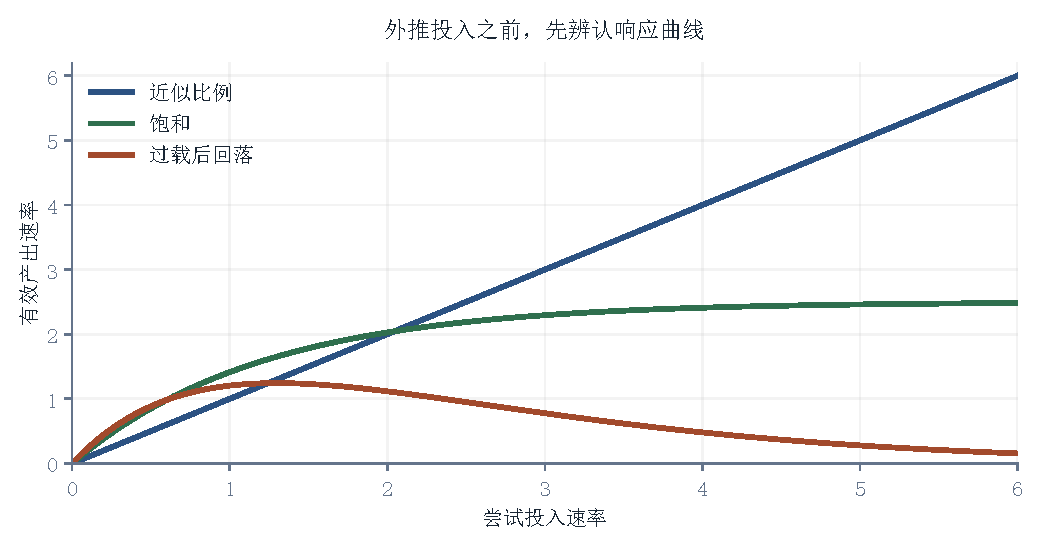
\includegraphics[width=\textwidth]{figures/response-regimes.pdf}
\caption{投入与有效产出可以近似成比例、逐渐饱和，也可以在过载后回落。曲线为机制示意，具体系统的形式与参数需要测量。}
\label{fig:mechanism-response-regimes}
\end{figure}
\subsection{速率失配与界面耗散}

\subhead{三套时钟不能同频}

上一节分开讲的三条响应谱之间，还有一个更隐蔽的问题：它们不能用同一种速度逻辑驱动。比特可以高频生成，原子需要功率匹配，生命需要弛豫时间。智能进入现实系统时，不只是进入不同介质，也是在穿过不同速率的界面。比特层可以在极短时间内计算、更新和传播；原子层有惯性、传热、摩擦、疲劳、执行器响应和安全边界；生命层还有代谢周期、免疫反应、组织修复、行为适应和长期反馈。输入层越快，越不能假定吸收层会同步变快。

这里会出现一种类似阻抗失配的现象。在工程系统中，源端与负载端如果阻抗不匹配，输入能量不能有效传入负载，反而会产生反射、损耗或振荡。这一关系的标准形式是反射系数
\begin{equation}
\Gamma=\frac{Z_L-Z_S}{Z_L+Z_S},\qquad \frac{P_{\mathrm{refl}}}{P_{\mathrm{in}}}=|\Gamma|^2
\end{equation}
这里以无损传输线接终端负载为例，$Z_S$表示实数正的特性阻抗，$Z_L$表示负载阻抗，单位为欧姆。$\Gamma$是电压反射系数，反射功率与入射功率之比为$|\Gamma|^2$；负载也取非负实数时，$\Gamma$位于$-1$与$1$之间。阻抗匹配使反射消失。智能系统中的输出频率、审核吞吐和执行能力各有单位，需另行测量；排队、丢弃、过调节和结构损伤则是失配可以直接观察的结果。

失配可以用输入速率与吸收能力之比描述。设$r=v_{\mathrm{in}}/v_{\mathrm{abs}}$，以吸收能力为单位记录有效推进量，另用损伤项描述超载后的退化：
\begin{equation}
r=\frac{v_{\mathrm{in}}}{v_{\mathrm{abs}}},
\qquad
u(r)=
\begin{cases}
r, & 0<r\le 1\\[3pt]
1-\kappa\,(r-1)^{m}, & r>1
\end{cases}
\label{eq:rate-mismatch}
\end{equation}
$v_{\mathrm{in}}$和$v_{\mathrm{abs}}$采用相同单位，$r$无量纲。$u$是净推进速率除以吸收能力所得的相对量。$r\le1$时输入全部被吸收，$u=r$表示能力尚未用满；$r>1$时，模型以$\kappa(r-1)^m$表示超载引起的净损失。$\kappa\ge0$、$m>0$须由观察确定，$u<0$表示损伤超过当期收益。若系统只排队而不退化，应改用饱和吞吐模型。信息网络、机械装置和生命系统都可能在超载后受损，差别须由具体机制与数据说明。

分层转换在工程系统里早有成熟的做法。电网的频率控制不是单一回路：一次调频由发电机组调速器在秒级自动完成，二次调频由调度中心在分钟级调整出力计划，三次调频和机组组合则在小时到天的尺度上重新排布。层级越慢，能调动的资源越多，代价也越高；把慢层的问题压给快层，系统会失稳，把快层的问题堆到慢层，则会积压。数据系统中的安排同类：写入先落到日志里，再由批处理合并进主存储，读取请求不会被要求等待所有维护动作完成。这些结构承认的都是同一件事，源端和负载端的速率不同，中间必须有人做转换，转换本身要消耗资源，但不做转换的代价更大。

成熟的 AI 系统不是把所有介质推向最高频率，而是建立跨介质的速率转换。真正的智能不是单纯提高源端输出，而是提高源端与负载端之间的匹配效率。AI 不一定失败在模型不够强，也可能失败在界面不匹配：输出太多，系统无法筛选；更新太快，流程无法吸收；控制太密，物理层开始振荡；干预太强，生命系统开始反弹；指标太频繁，组织开始内耗。\key{智能没有消失，而是在界面处被耗散了。}
\begin{figure}[ht]
\centering
% >>>>>>>>>> figs/fig-rate-mismatch.tex >>>>>>>>>>
% 图 3-2  速率失配：两侧都是浪费，只是浪费的形式不同
% 横轴是「输入速率 ÷ 介质吸收速率」的对数刻度，纵轴是有效转化率。
% 三条曲线对应三种介质：比特的吸收带最宽，原子次之，生命最窄。
% 左侧（输入慢于吸收）是产能闲置；右侧（输入快于吸收）是界面耗散——
% 堆积、发热、磨损。生命介质在右侧还跌破零：不是不转化，是被反噬。
% 坐标宏里不写括号（见 fig-three-media.tex 的注释）。
\begin{tikzpicture}[x=1cm, y=1cm, font=\small,
  ax/.style={-{Stealth[length=2.0mm]}, ink, line width=0.6pt},
  tk/.style={font=\scriptsize, text=slate, anchor=north},
  yk/.style={font=\scriptsize, text=slate, anchor=east}
]
\useasboundingbox (-0.35,0.95) rectangle (11.70,-5.60);

\def\aX{1.05} \def\aY{-4.00} \def\dx{1.70} \def\dy{2.85}
\def\px#1{\aX+\dx*2.5+\dx*#1}
\def\py#1{\aY+\dy*#1}

% ---------- 两侧失配区（先铺底）----------
\fill[deepblue!8] (\aX,{\aY-0.10}) rectangle ({\px{0}},{\aY+\dy*1.20});
\fill[rust!9]     ({\px{0}},{\aY-0.10}) rectangle ({\px{2.5}},{\aY+\dy*1.20});
\node[font=\scriptsize\heiti, text=deepblue!80, anchor=north] at ({\px{-1.35}},{\aY+\dy*1.16})
      {闲置：输入慢于吸收};
\node[font=\scriptsize\heiti, text=rust!85, anchor=north] at ({\px{1.30}},{\aY+\dy*1.16})
      {耗散：输入快于吸收};

% ---------- 坐标轴 ----------
\draw[ax] (\aX,\aY) -- ({\px{2.5}+0.30},\aY)
      node[anchor=south east, font=\scriptsize, text=ink, yshift=2pt] {输入速率 / 吸收速率};
\draw[ax] (\aX,\aY) -- (\aX,{\aY+\dy*1.24})
      node[anchor=south, font=\scriptsize, text=ink, yshift=1pt] {相对净推进量};
\foreach \e/\t in {-2.5/{$10^{-2.5}$},0/{$1$},2.5/{$10^{2.5}$}} {
  \node[tk] at ({\px{\e}},{\aY-0.10}) {\t};
}
\foreach \f in {0,0.5,1.0} {
  \draw[slate!55, line width=0.4pt] (\aX,\py{\f}) -- ({\aX-0.07},\py{\f});
  \node[yk] at ({\aX-0.09},\py{\f}) {\f};
}
% 零线（生命介质的代偿会跌破它）
\draw[slate!70, line width=0.6pt] ({\aX-0.05},\aY) -- ({\px{2.5}+0.30},\aY);
% 匹配线
\draw[slate!65, line width=0.6pt, dashed] (\px{0},\aY) -- (\px{0},{\aY+\dy*1.20});
\node[font=\scriptsize, text=slate, anchor=west] at ({\px{0}+0.09},{\aY+0.13}) {匹配};

% ---------- 三条响应曲线 ----------
\def\ptsA{}
\foreach \e/\f in {-2.5/0.10, -2.0/0.24, -1.5/0.43, -1.0/0.65, -0.5/0.83,
                   0.0/0.94, 0.5/0.90, 1.0/0.79, 1.5/0.65, 2.0/0.53, 2.5/0.43} {
  \pgfmathsetmacro{\xx}{\aX+\dx*2.5+\dx*\e}
  \pgfmathsetmacro{\yy}{\aY+\dy*\f}
  \xdef\ptsA{\ptsA\space(\xx,\yy)}
}
\draw[deepblue!85, line width=1.7pt] plot[smooth, tension=0.85] coordinates {\ptsA};

\def\ptsB{}
\foreach \e/\f in {-2.5/0.03, -2.0/0.10, -1.5/0.23, -1.0/0.44, -0.5/0.70,
                   0.0/0.90, 0.5/0.84, 1.0/0.65, 1.5/0.42, 2.0/0.26, 2.5/0.17} {
  \pgfmathsetmacro{\xx}{\aX+\dx*2.5+\dx*\e}
  \pgfmathsetmacro{\yy}{\aY+\dy*\f}
  \xdef\ptsB{\ptsB\space(\xx,\yy)}
}
\draw[terra!90, line width=1.7pt] plot[smooth, tension=0.85] coordinates {\ptsB};

\def\ptsC{}
\foreach \e/\f in {-2.5/0.01, -2.0/0.05, -1.5/0.14, -1.0/0.32, -0.5/0.60,
                   0.0/0.86, 0.4/0.86, 0.8/0.62, 1.2/0.22, 1.5/0.00,
                   2.0/-0.22, 2.5/-0.34} {
  \pgfmathsetmacro{\xx}{\aX+\dx*2.5+\dx*\e}
  \pgfmathsetmacro{\yy}{\aY+\dy*\f}
  \xdef\ptsC{\ptsC\space(\xx,\yy)}
}
\draw[forest!85, line width=1.7pt] plot[smooth, tension=0.85] coordinates {\ptsC};

% ---------- 曲线右端贴签 ----------
\node[font=\scriptsize, text=deepblue!85, anchor=west] at ({\px{2.5}+0.12},{\py{0.43}})
      {比特};
\node[font=\scriptsize, text=terra!90, anchor=west] at ({\px{2.5}+0.12},{\py{0.17}})
      {原子};
\node[font=\scriptsize, text=forest!85, anchor=west] at ({\px{2.5}+0.12},{\py{-0.34}})
      {生命};

% ---------- 读数：同一速率下差距可以很大 ----------
\draw[ink!50, line width=0.45pt, densely dotted] (\px{1.0},\aY) -- (\px{1.0},{\aY+\dy*0.79});
\draw[ink!50, line width=0.45pt, densely dotted] ({\px{1.0}},{\aY+\dy*0.79}) -- ({\px{0.0}},{\aY+\dy*0.79});
\node[font=\scriptsize, text=ink, anchor=north east, align=right]
      at ({\px{0.98}},{\py{0.76}}) {同一输入速率下\\净推进量可能不同};
\draw[ink!55, line width=0.5pt, {Stealth[length=1.4mm]}-{Stealth[length=1.4mm]}]
      ({\px{1.0}},{\aY-0.42}) -- ({\px{0.0}},{\aY-0.42});
\end{tikzpicture}

% <<<<<<<<<< figs/fig-rate-mismatch.tex <<<<<<<<<<

\caption{速率失配：两侧都是浪费，只是形式不同。横轴为输入速率与吸收速率之比，比值偏离中点越远，失配越大。三条曲线分属三种介质，可用带宽依次收窄；纵轴为相对净推进量，负值表示超载损伤超过有效推进；三条线采用不同示意参数。}
\label{fig:rate-mismatch}
\end{figure}


\subhead{介质适配}

因此，AI 时代成熟的智能观，不能只问模型能否输出更优结果，而要问输出如何被介质转译。它是否稳定，还是引发震荡？是否低耗，还是制造废热和维护负担？是否可控，还是触发生命与系统反弹？是否可验证，还是只在表示空间中看似成立？智能的边界不只在模型内部，也在介质响应之中。介质响应谱的意义，正在于纠正一种无介质的智能幻想：AI 不是把答案直接写进世界，而是把输出交给介质，比特会把它扩散，原子会要求它做功，生命会对它反馈，每一种转译都有成本，每一种响应都有边界，每一种吸收都有失败形式。

真正有效的智能系统，必须学会适配介质。面对比特，它要处理真实性和信任；面对原子，它要处理功率、耗散和维护；面对生命，它要处理反馈、弛豫和长期后果。它不能只会生成，还必须知道生成之后将被什么吸收；不能只会优化，还必须知道优化进入介质后会变成什么残余；不能只会加速，还必须知道何时需要降频、缓冲和验证。本章开头那句话到这里才算落到实处：智能不是直接改变世界，而是被介质转译，而 AI 的真实效能，取决于这种转译是否稳定、低耗、可控、可验证。

网络协议提供了同类经验的另一个版本。1980 年代中期的互联网出现过拥塞崩溃，从劳伦斯伯克利实验室到加州大学伯克利分校的一条链路，吞吐量一度从 32 千比特每秒掉到 40 比特每秒。Van Jacobson 和 Michael Karels 在 1988 年给出的解决办法不是在接收端扩容，而是给发送端加一个拥塞窗口：发送端在收到确认之前只能发送有限的数据，丢包被解释为路径拥塞的信号，窗口随之减半，平稳时再缓慢增长\cite{jacobson1988}。这个设计承认的正是源端必须服从吸收端。如果发送端只按自己的输出能力推进，中间节点的队列会先被填满，然后开始丢弃，两端重传进一步加重负担，系统的有效吞吐量反而下降。协议的自律不是道德要求，而是把介质的带宽写进了源端的控制律。

但介质并不是等待被适配的空白材料。每一种介质都有自己的历史，它被制造出来的时候，参照的是人的身体、既有的工艺和当时的制度，而不是智能的输入格式。智能进入这样的介质时，真正的问题往往不是转译发生在哪一层，而是能不能在不改动介质骨架的条件下完成转译；而骨架一旦需要改动，代价就要按原子世界的方式支付。

\section{演化策略：赛博寄生与复杂度棘轮}

智能要改变的现实，在它到达之前就已经建成。道路、楼宇、医院和工厂各有既存结构，也嵌入法规、保险、习惯与责任安排。模型要通过这些接口工作，部署成本便取决于需要改动多大的范围。换一个部件是维修，换一套承重结构是重建。单点能力足够以后，还要比较适配旧结构与重建环境的总成本。

\subsection{覆盖层策略与重构的三重代价}

\subhead{重构的三重代价}

理论上，最干净的道路是重构底层。为自动驾驶重新设计道路、车辆、信号、保险和交通规则；为机器人重新设计楼宇、工具、仓库、家庭和工厂；为智能医疗重新设计医院流程、病历结构、责任制度和支付体系。这样，物理世界本身会变得更适合机器感知、机器行动和机器决策，系统会更低熵，接口会更清楚，反馈会更稳定。但这条路太贵。

彻底重构原子世界需要克服三重代价。第一是资源势垒：道路、工厂、医院、港口、电网、住宅和城市管网已经沉淀了巨大的材料、资本、空间和劳动，推倒重建，不是修改代码，而是废弃既有物质结构并重新支付能量账单。第二是时间刚性：基础设施有自己的寿命周期，施工、审批、迁移、协调和行为改变都不能像软件版本一样即时更新。第三是拓扑耦合：道路不只是道路，它连接保险、法规、物流、地产、职业分工和居民生活，医院不只是建筑，它连接医生责任、患者信任、医保支付和法律边界。改动底层，就会牵动整个系统。

水泥、钢铁与设备的大规模年度产出，逐年沉积为建筑、道路、厂房和网络。USGS与世界钢铁协会的2026年报告仍显示，全球水泥与粗钢产出分别处在数十亿吨与近二十亿吨的量级。\cite{usgs2026cement,worldsteel2026figures} 存量改造取决于寿命、替换率、建设能力和相邻系统；不能把某一年的产量直接等同于可同时改造的存量。

这三重代价不是新出现的东西，它们正是上一章那三项在建成环境中的具体形式。资源势垒对应已经支付出去的材料、能量和空间成本，时间刚性对应基础设施无法压缩的过程时长，拓扑耦合对应道路、法规、保险和职业分工之间已经形成的连接密度。一个已经建成的东西，它的黏滞不是被谁后来加上去的，而是在建成那一刻就写进了结构。因此，判断一项智能改造是否可行，不能只看它在符号空间里节省了多少，还要看它在多大范围内要求这套旧结构重新支付一次。

\subhead{覆盖层策略}

所以文明通常不会优先选择重构，而会选择覆盖。所谓\term{覆盖层策略}，是指在不彻底改变旧物理骨架的情况下，在其表面叠加一层新的比特控制层。道路不变，加导航、摄像头、雷达、高清地图和云端训练；工厂不变，加传感器、预测维护、数字孪生和调度平台；医院不变，加影像识别、病历摘要、智能分诊和审核系统；城市不变，加摄像头、平台、算法、数据接口和“智慧治理”。原子骨架保持沉重，数字薄膜覆盖其上。

这是一种赛博寄生。这里的“寄生”不是道德意义上的贬义，而是一个结构描述，也是一种演化策略：新的智能层并不独立存在，也不立即替换旧层，而是依附在旧物理系统之上，利用其已经形成的空间、能源、设备、制度和人员网络，获得进入现实的行动位置，并试图改变旧系统的行为。比特层像一层神经组织，覆盖在旧世界的骨架上；它不替换骨骼，却试图让骨骼行动得更快、更准、更可调度。

这种策略之所以普遍，是因为它符合最小代价原则。彻底重构世界太重，局部覆盖则轻得多：加装传感器比重建道路便宜，开发调度系统比重建工厂便宜，训练识别模型比重写医疗制度便宜，给机器人增加感知和控制能力比重新设计全部生活空间便宜。覆盖层是一种绕过高黏滞底层的次优解，它不解决底层沉重性，而是在沉重性上方寻找可操作空间。短期看，覆盖层非常有效：用户端更顺滑，管理端更可视，调度更实时，风险更可监控，局部效率确实提高。一个旧系统被数字化后，看起来像是变轻了，司机有导航，工厂有预测维护，医生有辅助诊断，城市有监控平台，仓库有自动分拣，许多原本依赖人工经验和局部判断的流程，被新的比特层重新组织。

覆盖并不是数字时代才有的策略。19 世纪末到 20 世纪初，工厂的动力从蒸汽机集中传动改为电动机分散驱动，技术替换在 1890 年代就已大规模展开，但生产率的大幅提升要等到厂房布局、传动方式、机器排布和生产组织都围绕分散动力重排之后才出现，中间隔了二三十年。集装箱的推广同样如此：1956 年第一次集装箱运输之后，码头、起重机、卡车底盘、铁路平车、仓储布局、工会规则和关税制度都要跟着改，港口装卸区被整体搬迁，直到 1970 年代集装箱化才真正铺开。两者都说明，新层接入旧骨架时，瓶颈往往不在新层本身，而在旧骨架愿不愿意为它改变。

近年的例子更容易看清覆盖层的收益边界。2019 年起全国推广高速公路电子不停车收费，江苏、山东、四川、重庆的试点统计显示，客车通过省界的时间从 15 秒降到 2 秒，货车从 29 秒降到 3 秒；2020 年 1 月 1 日，全国 29 个联网省份的 487 个省界收费站全部取消。收费站这个环节确实被比特层改写了，但车道数、匝道容量、主线通行能力和服务区容量都没有随之改变。节假日的高峰流量仍然要在同样的物理通道里消化，拥堵从收费站前移到了主线和出入口。当收费站不再是瓶颈，瓶颈会回到骨架本身上来。这笔收益是真的，但它只在骨架允许的范围内兑现。

旧世界之所以沉，还因为它把一批历史决定固化成了物理尺寸。铁路轨距在 19 世纪被定在 1435 毫米，此后隧道、桥梁、站台和车辆全部按这个宽度建造。集装箱在 1960 年代被定在 20 英尺和 40 英尺两个长度，港口的起重机跨距、堆场分区、卡车底盘和铁路平车随之定型。楼梯踏步的高度上限、住宅门洞的宽度档位、插座形状、交流电频率、键盘字母排布，都是按当时的人体尺度、工艺条件和行业妥协定下来的。这些东西今天还在用，不是因为它们最优，而是因为改动它们的代价要按原子世界的方式支付，并且要由整条链条分摊。

覆盖层策略之所以普遍，还因为它把成本记在了另一个账本上。加装传感器、部署摄像头、上线调度平台，这些支出落在当年的资本开支和运维预算里，看得见也算得清；而旧骨架没有为机器感知和机器行动改变过这件事，不会被计入任何一项成本。前者是显性支出，后者是隐性欠账。短期看，覆盖层的收益立刻显现，一个旧系统被数字化之后确实变顺滑了。代价要等到覆盖层之间开始互相依赖时才出现，而那时它已经变成了维持运行的必要条件。

\subsection{复杂度棘轮、兼容税与落地税}

\subhead{复杂度棘轮}

覆盖层需要传感、数据、通信、权限、监控、维护与异常处理。新增接口若同时要求旧结构作出配套，局部收益可能带来新的耦合；结构又依赖更多结构来维持时，就形成\term{复杂度棘轮}。模块化、标准化和淘汰旧接口也能让复杂度净下降，具体方向要从架构与运行记录判断。

这个过程可以写成一个递推关系
\begin{equation}
C_{n+1}=(1+\alpha)\,C_n+c
\label{eq:ratchet-recursion}
\end{equation}
其中$C_n$为按一致口径统计的复杂度，$c$为新增层的直接增量，$\alpha$为既有结构因新层接入而增加的比例。固定$c>0$、$\alpha>0$时，这个递推给出指数增长；$\alpha=0$时为线性增长。它描述依赖持续累积的一种情形，不能由层数本身推定实际系统服从固定比例。

把 \eqref{eq:ratchet-recursion} 展开，可以看清棘轮的形状。设起始复杂度为 $C_{0}$，$n$ 层之后
\begin{equation}
C_{n}=(1+\alpha)^{n}C_{0}+\frac{c}{\alpha}\bigl[(1+\alpha)^{n}-1\bigr],
\qquad
C^{\min}_{n}=\beta\,C_{n},\qquad 0<\beta<1
\label{eq:ratchet-floor}
\end{equation}
$\alpha>0$时第一式给出递推解；$\alpha=0$时取极限$C_n=C_0+nc$。第二式把拆除后仍保留的复杂度记为当前值的$\beta$倍，$\beta$需要由具体退出方案估计。旧依赖可以被移交、重构或清除，因此$C_n^{\min}$是情景下的可达水平，不是普遍物理下限。

这个差就是锁定带，它的累积量就是卸载前 $n$ 层要付的兼容税
\begin{equation}
K_{n}=\sum_{k=1}^{n}\bigl(C_{k}-C^{\min}_{k}\bigr)=(1-\beta)\sum_{k=1}^{n}C_{k}
\label{eq:compat-tax}
\end{equation}
$K_n$把逐层差额汇总成一个兼容负担指标，单位随复杂度口径确定。各层有共享接口时，直接相加会重复计算；转换为退出费用，需要分别估计拆除、迁移、验证与替代支持。实际成本也可能在集中重构时下降，不能只凭这个和式断言退出账单必然指数上升。

自动驾驶正是覆盖层困境的典型案例\cite{kalra2016}。道路原本不是为机器视觉设计的，交通规则原本不是为算法责任设计的，保险制度原本不是为无人主体设计的，行人和司机也不会完全按照机器协议行动。自动驾驶如果要真正简单，最合理的办法是重构环境：封闭道路、人车分流、统一车路通信、标准化交通参与者、清晰责任边界，但这意味着重构城市交通的底层，代价极高。于是自动驾驶选择覆盖层路线：不改造所有道路，而是让车携带更多传感器；不要求所有人类行为标准化，而是让算法处理长尾；不立即重写责任制度，而是叠加安全员、远程接管、监管沙盒、保险补丁和数据记录。环境没有变简单，车辆只能变复杂；道路没有被低熵化，算法只能承受更多不确定性。自动驾驶看似是机器替代司机，深层上却是把道路重构成本转移到了单车智能、感知冗余、云端训练和责任系统中。这也是为什么人机混行阶段格外困难：纯人类驾驶是一种相对稳定的旧秩序，纯机器驾驶在高度标准化环境中也可能稳定，最复杂的是二者混合的过渡态，人类、机器、旧道路、旧法规、非标准行为、保险责任和社会预期同时存在，系统进入高熵混合区。此时智能越强，不一定系统越简单，很多算力其实是在为旧环境的无序性买单。
\begin{figure}[ht]
\centering
% >>>>>>>>>> figs/fig-ratchet.tex >>>>>>>>>>
% 图 3-3  复杂度棘轮：能加不能减的那一部分
% 横轴时间，纵轴系统复杂度。实线是当前复杂度，每加一层上一个台阶；
% 虚线是可回退的下限——它也在涨，只是涨得慢。两线之间是锁定带：
% 想退回上一代，得先付清这一带里的兼容税。台阶越多，带越宽。
% 末端点划线是「只覆盖不重构」的外推：层继续堆，可回退下限抬得更快。
\begin{tikzpicture}[x=1cm, y=1cm, font=\small,
  ax/.style={-{Stealth[length=2.0mm]}, ink, line width=0.6pt},
  arr/.style={{Stealth[length=1.5mm]}-{Stealth[length=1.5mm]}, ink!60, line width=0.5pt}
]
\useasboundingbox (-1.05,0.80) rectangle (12.85,-6.05);

\def\aX{1.15} \def\aY{-4.45} \def\dx{0.98} \def\dy{0.40} \def\aR{11.30}
% 坐标宏里不写括号，见 fig-three-media.tex 的注释
\def\px#1{\aX+\dx*#1}
\def\py#1{\aY+\dy*#1}

% ---------- 锁定带：上界走台阶，下界走缓坡，两界之间填色 ----------
\fill[rust!13]
  (\px{0.4},\py{0.55}) -- (\px{1},\py{0.55}) -- (\px{1},\py{1.90})
  -- (\px{2},\py{1.90}) -- (\px{2},\py{3.00}) -- (\px{3},\py{3.00})
  -- (\px{3},\py{4.10}) -- (\px{4},\py{4.10}) -- (\px{4},\py{5.30})
  -- (\px{5},\py{5.30}) -- (\px{5},\py{6.40}) -- (\px{6},\py{6.40})
  -- (\px{6},\py{7.60}) -- (\px{7},\py{7.60}) -- (\px{7},\py{8.80})
  -- (\px{8},\py{8.80}) -- (\px{8},\py{10.10}) -- (\px{9.6},\py{10.10})
  -- (\px{9.6},\py{1.62})
  -- (\px{8},\py{1.42}) -- (\px{6},\py{1.18}) -- (\px{4},\py{0.95})
  -- (\px{2},\py{0.85}) -- (\px{0.4},\py{0.40}) -- cycle;

% ---------- 坐标轴 ----------
\draw[ax] (\aX,\aY) -- (\aR,\aY) node[anchor=west, font=\scriptsize, text=ink] {时间};
\draw[ax] (\aX,\aY) -- (\aX,\py{10.9})
      node[anchor=south, font=\scriptsize, text=ink, yshift=1pt] {系统复杂度};

% ---------- 实线：当前复杂度 ----------
\draw[deepblue!85, line width=1.9pt]
  (\px{0.4},\py{0.55}) -- (\px{1},\py{0.55}) -- (\px{1},\py{1.90})
  -- (\px{2},\py{1.90}) -- (\px{2},\py{3.00}) -- (\px{3},\py{3.00})
  -- (\px{3},\py{4.10}) -- (\px{4},\py{4.10}) -- (\px{4},\py{5.30})
  -- (\px{5},\py{5.30}) -- (\px{5},\py{6.40}) -- (\px{6},\py{6.40})
  -- (\px{6},\py{7.60}) -- (\px{7},\py{7.60}) -- (\px{7},\py{8.80})
  -- (\px{8},\py{8.80}) -- (\px{8},\py{10.10}) -- (\px{9.6},\py{10.10});
% ---------- 虚线：可回退下限 ----------
\draw[forest!85, line width=1.4pt, dashed]
  (\px{0.4},\py{0.40}) -- (\px{2},\py{0.85}) -- (\px{4},\py{0.95})
  -- (\px{6},\py{1.18}) -- (\px{8},\py{1.42}) -- (\px{9.6},\py{1.62});

% ---------- 各层之间的分界（细点线，只在锁定带里画）----------
\foreach \k in {1,3,5,7} {
  \draw[slate!45, line width=0.4pt, densely dotted]
        (\px{\k},\py{0.8}) -- (\px{\k},\py{9.2});
}

% ---------- 注记 ----------
\node[font=\scriptsize, text=deepblue!85, anchor=south west] at (\px{4.35},\py{5.42})
      {当前复杂度：每加一层，上一个台阶};
\node[font=\scriptsize, text=forest!85, anchor=north west] at (\px{0.45},\py{0.30})
      {可回退下限};
\node[font=\scriptsize, text=slate, anchor=south] at (\px{1.5},\py{1.98}) {第一层};
\node[font=\scriptsize, text=slate, anchor=south] at (\px{4.5},\py{4.18}) {第二层};
\node[font=\scriptsize, text=slate, anchor=south] at (\px{6.5},\py{6.48}) {第三层};
\node[font=\scriptsize, text=slate, anchor=south] at (\px{7.6},\py{8.88}) {第四层};

% 锁定带厚度
\draw[arr] (\px{9.30},\py{1.62}) -- (\px{9.30},\py{10.10});
\node[font=\scriptsize, text=ink, anchor=west, align=left] at (\px{9.40},\py{6.40})
      {锁定带\\（兼容税）};

% 末端外推
\draw[ink!60, line width=1.0pt, densely dashdotted]
      (\px{9.6},\py{10.10}) -- (\px{10.7},\py{11.35});
\node[font=\scriptsize, text=ink, anchor=north west, align=left]
      at (\px{9.65},\py{10.02}) {只覆盖\\不重构};
\end{tikzpicture}

% <<<<<<<<<< figs/fig-ratchet.tex <<<<<<<<<<

\caption{复杂度棘轮。两条线的间距即锁定带：想退回上一代，得先付清这一带里的兼容税。带的两侧都在上涨，但涨速不同，间距因此逐级拉开；台阶越多，带越宽。}
\label{fig:ratchet}
\end{figure}


\subhead{兼容税与落地税}

具身智能面对的是同一种赛博寄生，只是空间更广。家庭、医院、餐厅、仓库、商场和街道，都不是为机器人身体设计的：门把手默认人手，楼梯默认双腿，厨房默认眼手协调，工具默认人的触觉和常识，家庭物品默认人类的模糊处理能力。机器人要进入这些空间，就必须支付兼容税：更多自由度、更复杂传感器、更高实时控制、更强安全冗余、更昂贵维护体系。工业机器人之所以成功，是因为它们通常被放在低熵环境中，固定位置、重复动作、标准物料、隔离空间、明确任务；通用具身智能之所以困难，是因为它要进入高熵人类环境，这里物体位置不固定，任务目标含糊，空间布局多样，人类行为不可预测，接触反馈复杂。给机器人装上大模型，并不会自动取消摩擦、碰撞、误差、遮挡、材料差异和责任风险。

这种成本分布有一个更早的表述。Hans Moravec 在 1988 年指出，让计算机在智力测验或下棋上达到成人水平相对容易，要让它在感知和运动上达到一岁儿童的水平却极其困难\cite{moravec1988}。这个判断在三十年后的具身智能研究中仍然成立：需要显式推理的任务可以被形式化、被标注、被搜索，而抓取、行走、避障这类能力依赖大量隐性调节，只能在接触中训练出来，训练成本恰好落在最不容易复制的那一部分。兼容税之所以高昂，不是因为机器人不够聪明，而是因为它要补的正是人类身体用漫长演化预先支付掉的那部分调节。

所谓“落地税”，就发生在模型接触现实的一瞬间。任何世界模型都是现实的压缩，而现实总有残差，模拟器中的训练无法穷尽真实世界的高频噪声、边缘情况、材料变化和人类偶然性。机器人一旦行动，就会改变被建模对象：拿起杯子，杯子位置变了；推开门，门的状态变了；进入房间，人的行为也可能变了。物理AI不是在静态地图上执行，而是在被自己扰动的环境中连续修正。因此，覆盖层物理AI的真正难点，不是智能不足，而是旧世界没有为智能低成本行动而重构。AI必须在旧世界中支付兼容税、残差税和维护税。它通过比特层提高局部效率，却不得不承担原子层的沉重、混乱和不可回滚后果。

\subhead{覆盖与重构之间}

覆盖层策略的问题，不在于它无效，而在于它容易被误认为重构。覆盖可以延长旧系统生命，可以提高局部效率，可以让旧基础设施获得新的控制能力，但覆盖不能无限叠加。每加一层，都要问：它减少的摩擦，是否大于它增加的复杂度？它节省的人力，是否小于它带来的维护负担？它提升的效率，是否值得它增加的脆弱性？一个系统如果只覆盖、不重构，就会逐渐形成高效而脆弱的复杂网络。正常运行时，它显得极其智能；一旦接口失效、数据异常、传感器故障、平台宕机或责任链断裂，复杂性就会反过来成为风险放大器。旧系统的问题没有消失，只是被更多智能层遮住；旧责任没有消失，只是被平台、算法、运营者、用户、监管者和人工兜底重新分散。

所以，物理AI的成熟，不只是让模型更大、传感器更多、控制更精细，而是判断何时覆盖，何时重构，何时放弃。低风险、低耦合、高标准化场景适合覆盖：封闭园区、工业产线、仓储物流、固定路线运输，都可以通过覆盖层获得明显收益。高风险、高开放、高耦合场景不能只靠覆盖：自动驾驶、医疗护理、家庭机器人、城市治理，最终都需要环境设计、制度重构和责任边界的同步变化。未来的物理AI竞争，不只是模型能力之争，而是环境低熵化能力、接口标准能力、基础设施重构能力和责任制度设计能力之争：谁能减少兼容税，谁就能让智能行动更便宜；谁能降低环境混乱度，谁就能让具身系统更可靠；谁能识别覆盖与重构的边界，谁就能避免复杂度棘轮把系统拖向脆弱。赛博寄生是物理AI的起点，不是终点。AI进入原子世界，往往先作为覆盖层寄生在旧系统之上；但如果永远停留在覆盖层，文明只会得到越来越复杂的补丁网络。真正可靠的物理智能，不是无止境地给旧世界贴上传感器和算法，而是在覆盖、重构和保留之间找到最低总黏滞的路径。

旧世界不会因为智能到来而自动消失。它会先被覆盖、被监控、被调度、被补丁化。物理AI的第一性现实就在这里：智能要改变原子世界，必须先寄生原子世界；而它最终能否成熟，取决于它是否有能力从寄生走向真正的环境重构。但无论选择覆盖还是重构，智能都在持续向一个高黏滞系统输入。系统未必按输入的方向改变：它可能沿阻力更低的路径绕开，可能把吸收不了的输入堆在自己内部，也可能因为反馈过急而开始摆动。这三种反应不受策略选择支配，只受系统自身动力学的支配。

\section{动态响应形态：绕行、堆积与失稳}

智能输入并不因为它来自系统外部就获得优先权。输入进入系统之后，会被这个系统自身的动力学重新处理：有的被吸收，有的被推迟，有的被放大。覆盖层增加的是结构，结构增加的是界面，而界面越多，输入转化为有效改变的路径就越长。

\subsection{概率捷径与绕行}

智能进入现实系统之后，并不会只有一种结果。它有时能找到低阻路径，使原本困难的问题突然出现新的解法；有时会在系统界面处发生堆积，输入越来越多，真实改变却没有同步增加；有时还会因为反馈延迟和过度修正，引发震荡，使系统变得更不稳定。这三种形态，可以概括为：绕行、堆积与失稳。但它们并不完全站在同一条轴上。绕行是智能避开壁垒的策略，是输入穿过阻力之后的成功响应；堆积与失稳，则是智能硬推高黏滞系统时的两种失败响应，输入太多，系统吸收不了，就堆积，控制太急，反馈来不及，就失稳。因此，所谓三种响应，不是三个并列失败模式，而是智能输入进入现实后的三种命运：穿过去，堵在中间，反弹成波动。

资源势垒、时间刚性、拓扑耦合和介质的响应方式，说明的是现实系统为什么有阻力；这里要进一步看的，是当智能持续输入一个有阻力的系统时，系统会如何运动。高黏滞系统不是一堵静止的墙，而是一个会吸收、过滤、延迟、堆积、反弹和放大的动态场。AI 时代最常见的误判，是把智能输入看成一种单向加速力量，似乎模型越强，系统就越快；方案越多，进步就越快；预测越频繁，决策就越优；控制越密集，现实就越可控。但现实系统不是被动接受输入的屏幕，它有资源上限，有过程时间，有结构路径，有反馈延迟，有安全边界，智能输入进入其中，可能变成有效改变，也可能变成库存、拥堵、波动和震荡。因此，判断 AI 的现实效果，不能只看它生成了多少方案，也不能只看它局部指标是否提高，更关键的问题是：这些输入进入系统之后，被转化成了什么动态形态？

\subhead{绕行：把试错挪进信息空间}

第一种形态是绕行。所谓绕行，是指智能并不正面击穿现实壁垒，而是在状态空间中寻找较低阻力的路径。面对高资源势垒和高拓扑耦合，最直接的路线往往并不是最可行的路线，现实中的许多困难，不是因为目标无法描述，而是因为从当前状态直达目标状态的代价太高。智能的价值，常常不是硬推过去，而是找到一条更少撞墙的路。

这就是\term{概率捷径}的意义。所谓概率捷径，不是魔法，也不是物理壁垒突然消失，它指的是：智能系统利用模型、模拟、搜索和组合能力，在大量可能路径中筛掉明显无效的路线，保留少数更有希望的路线，从而减少现实世界中的昂贵试错。它把一部分原本需要在物质世界中支付的成本，转移到信息空间中提前支付，现实试错仍然存在，但被压缩、重排和剪枝。AlphaGo 的“妙手”就是比特域中最容易理解的例子\cite{silver2016mastering}，它并没有改变围棋规则，也没有击穿棋盘的物理限制，而是在巨大的状态空间中找到人类经验较少抵达的低阻路径。它的反直觉之处，不在于违反规则，而在于重新组织了搜索空间：人类看似自然的路径，未必是全局上更好的路径，智能通过大规模搜索，发现了经验之外的可行通道。

用抽样代替求解的做法比深度学习早得多。1946 年，Stanis{\l}aw Ulam 在洛斯阿拉莫斯处理中子扩散问题时意识到，与其解析求解一个高维积分，不如反复随机抽样再统计结果，他和冯·诺依曼把这类方法命名为蒙特卡洛。它没有减少任何一次抽样的代价，却把“必须求出解析解”换成了“需要多少次抽样才够”。天气预报后来也从单一确定性解转向集合预报，用多组受扰动的初值给出概率分布，等于承认某些尺度的演化本来就无法精确预测。这类方法的共同点，是把原本要在现实里付出的试错，换成在受控随机过程中付出的计算，而随机过程可以重放、可以批量并行、可以在不损坏任何东西的条件下失败。

在原子世界中，类似机制也存在，只是代价更重。新材料发现、药物候选筛选、结构优化、工艺参数搜索，都可以看成在高维状态空间中寻找低阻路径，AI 可以帮助研究者少做一部分无效实验，避开明显失败的组合，把有限实验资源集中到更有希望的区域。但这仍然不是取消物理账本：候选材料必须合成，药物必须验证，工艺必须稳定，产品必须维护，智能减少的是盲目性，不是消除现实性。半导体工业中的计算光刻、工艺参数优化和缺陷控制，也体现了类似逻辑，微观制造越接近物理边界，直接缩放越来越困难，工程系统不是让微观物理边界消失，而是通过计算、控制和复杂工艺，在越来越狭窄的可行窗口中寻找可制造路径。这里的所谓进步，不是物理限制被抹除，而是直接路径受阻后，系统用更复杂、更昂贵、更低容错的方式继续绕行。

绕行也有绕不过去的地方，能量密度就是其中之一。航空煤油的比能量约为 12000 瓦时每千克，当前可商业化的锂离子电芯约为 250 到 300 瓦时每千克，两者相差约四十倍。把热机约三分之一的效率和电机百分之九十以上的效率折进去，差距仍然在十倍以上。这个势垒决定了几种绕行策略的可行边界：纯电动机动化在地面交通中可以借助轻量化、补能网络和路线约束绕开一部分代价，而在航空中，同样的绕行会被起飞重量直接罚回来，电池在整个航程中不减轻重量，燃油则在飞行中持续消耗。绕行能否成立，取决于它选择转移的那部分代价，是否小于它在新介质中新增的代价；一旦后者更大，绕行就只是把障碍换了一个位置。

蛋白质结构预测是同一逻辑在更大规模上的重演。从氨基酸序列到三维结构的映射空间极大，实验解析一个结构往往需要数月到数年，而预测模型把已知结构的统计规律压缩进参数，使候选结构的生成成本下降几个量级。但生成成本的下降并不等于确认成本的下降，任何一个预测出来的结构仍然要由实验测定或功能验证来承认，被预测出来的部分越多，需要排队确认的部分也越多。

生命系统中的绕行更加微妙。药物设计、基因编辑和合成生物学常常试图在生命网络中寻找可干预路径，真正有效的干预，并不一定是对系统施加强力，而是找到一个能以较低扰动改变整体状态的杠杆点。但生命系统有代偿、冗余和反馈：一个看似低阻路径，可能在短期有效，长期被系统抵消；一个罕见突变路径，可能提供治疗机会，也可能带来不可预期风险。生命中的概率捷径，必须比原子世界更加依赖验证。所以，绕行的本质不是减少全部代价，而是改变代价的支付结构。它把集中代价变成分散风险，把物理试错的一部分转移到模拟和搜索，把正面重构的一部分转化为路径选择。成功的绕行会显得像突然降阻，但它通常不是总作用量消失，而是路径重排之后，系统找到了更可承受的支付方式。

\subsection{堆积、库存与波动}

\subhead{堆积与库存化}

第二种形态是堆积。如果绕行是智能找到了较低阻力的路径，那么堆积就是智能输入超过了系统吸收能力，系统不是没有输入，而是输入太多；不是没有活动，而是活动不能转化为有效改变。表面上，系统更忙、更密集、更自动化、更实时，真实状态却没有同比变化。堆积发生在输入流大于吸收流的时候：一个系统可以接收多少方案、多少指令、多少资本、多少实验、多少指标、多少模型建议，并不取决于输入端能产生多少，而取决于执行、验证、协调和责任系统能吸收多少。超过这个吸收带宽，更多输入不会自动变成更多产出，只会在界面处排队、淤积、返工、内耗，或者退化为维护负担。

这个关系可以用存量方程表示
\begin{equation}
\frac{\mathrm{d}S}{\mathrm{d}t}=I(t)-A(S),\qquad A(S)\le A_{\max}
\end{equation}
$S$ 是系统界面处的存量，用待办事项、队列长度或未验证候选数计量；$I(t)$ 是输入速率，量纲为件/单位时间；$A(S)$ 是吸收速率，$A_{\max}$ 是吸收带宽，即执行、验证和协调系统在给定资源下单位时间能够处理的最大量。当 $I>A_{\max}$ 时，$A(S)$ 已经在饱和区，存量按 $S\approx(I-A_{\max})t$ 线性增长，这就是库存化；界面上的等待时间随存量上升，为 $S/A_{\max}$。压低 $I$ 是限流，提高 $A_{\max}$ 是扩容，两者的区别在于动的是输入端还是吸收端，而只有后者才改变系统的长期吞吐量。

堆积的第一种形态，是库存化。系统把无法及时吸收的输入暂时存起来，形成库存、队列、待办、积压、未验证候选和未处理风险。库存看似只是缓冲，实际上是时间刚性的显影：它说明输入已经抵达，但系统还没有能力把它转化为真实改变，库存越多，系统越不像在加速，越像在把未来的处理压力提前堆到某个界面上。在信息系统中，库存表现为筛选负担：AI 可以生成大量文本、图像、代码、方案和候选假设，但人类和组织的判断能力没有同步扩展，内容越多，审核越重，候选越多，验证越重，建议越多，决策越难。过去稀缺的是生成能力，现在稀缺的是确证能力，生成端的加速，如果没有验证端的扩容，就会形成信息堆积。在科研和工程系统中，库存表现为发现与验证之间的裂缝：高通量实验、自动化平台和 AI 搜索可以扩大候选空间，但很多结果仍要经过实验重复、稳定性测试、机理解释、工艺放大和长期可靠性验证，药物研发尤其明显，AI 可以帮助发现靶点、生成分子、筛选候选，但候选进入药物事实，仍要穿过毒理、药代、剂量、人群差异、临床试验和监管审查。更多候选不自动等于更多可靠药物，发现端越快，验证端越成为瓶颈。这不是说高通量和 AI 没有价值，而是说它们改变了瓶颈位置，它们减少了一部分早期搜索成本，却可能把系统压力推向后端验证、资源分配和失败筛选：一个系统如果只扩大发现能力，不扩大验证能力，就会出现候选堆积，它看起来更有创新活力，实际可能有大量可能性停在中间层，无法成为可靠结果。在组织系统中，库存表现为内耗，算力、资本、指标和指令可以快速注入，但组织学习、判断、执行和责任形成都有较低带宽，一个组织如果持续接收新的模型建议、实时指标、战略口号、优化方案和管理任务，却没有相应吸收能力，就不会自动变得更智能，它可能只是变得更忙，更多会议、更多报表、更多试点、更多汇报和更多短期目标，可能只是输入在组织界面处堆积。

所谓内耗，可以理解为输入无法转化为有效功。系统获得了更多信息、更多资源、更多竞争压力，但实体结构的响应能力没有同步提高，于是能量不能向外完成状态改变，只能在系统内部循环，它表现为重复协调、指标追逐、局部竞争、审核拥堵、注意力耗散和维护负担。这里的“热”不是严格物理意义上的热，而是高强度输入无法形成有效产出时留下的无效运动。

\subhead{波动与周期}

堆积并不总是静静堆在那里。输入超过吸收能力之后，系统首先形成存量；存量如果不能被局部消化，就会沿着结构传播。交通系统中，车辆继续向前行驶，堵塞波却可能向后传播；组织系统中，任务继续向下游分发，未决事项却会向上游管理层回涌；技术系统中，候选方案继续产生，验证瓶颈却会反向压缩前端搜索策略。这里真正移动的不是实体本身，而是无法被吸收的状态。这可以称为堆积波。堆积波不是交通系统的特殊现象，而是高黏滞系统的一般响应：当局部通道达到容量上限，系统会把无法吸收的流量转化为空间上的压力波，个体仍在向前，压力却可能向后传；任务仍在推进，瓶颈却可能反压前端；智能仍在生成方案，验证负担却会反过来限制搜索方向。高黏滞系统中的波，往往不是物质波，而是吸收失败的传播。

当系统要调节的不是轻变量，而是存量，堆积就可能变成周期。库存、产能、厂房、团队、城市、制度，都不是瞬间生成、也不是瞬间清除的东西：系统看到不足，于是扩张，等扩张形成真实供给时，环境可能已经变化；系统看到过剩，于是收缩，等收缩完成时，新的不足可能又出现。这里的问题不一定是控制者太急，而是被调节的存量太重，世界回应得太慢。周期不是时间自己在震荡，而是不同重量的存量在用不同速度纠错。

短周期常常来自轻存量。商品库存、待办任务、内容审核、候选方案，都可以较快增加，也可以较快清理，它们的周期短，是因为存量轻，反馈来得较快，修正也较快显影。可是即使是轻存量，只要信号滞后，修正也会过头，供应链中的牛鞭效应就属于这一类：终端需求的微小变化，经过订单、库存、生产和采购层层传递，会被信息延迟和存量调整逐级放大\cite{lee1997information}。中周期来自更重的存量：设备、产能、团队、厂房、供应链、资本开支，不是几天几周能改变的东西，系统看到需求上升，于是投资扩张，等新产能形成时，需求可能已经变化，系统看到过剩，于是收缩，等收缩完成时，新的不足可能又出现，这里调整的不是普通库存，而是生产能力本身，产能是更重的库存，因此周期更长，修正代价更高。更长的周期来自空间和结构存量：建筑、城市、道路、学校、医院、住房、基础设施，一旦建成，就很难快速回滚，它们把某一时期的预期固化为现实空间，等人口、产业、财政和生活方式改变时，空间不会立刻跟着改变，于是，一座城市可能在需求高涨时扩张，在需求转弱后留下过剩建筑、债务和低利用率基础设施，这里的周期不是普通波动，而是沉没结构的迟滞回声。最长的波动来自技术范式、能源系统和制度结构：一个新技术范式出现时，资本、基础设施、教育、监管、组织和生活方式都会围绕它重新配置，最初是扩张和想象，随后是过剩和筛选，再之后是清算、重组和稳定吸收，这样的长波不是精密钟表，也不是必然律，而是重结构在历史尺度上的重估和再耦合。

因此，不同周期未必是彼此无关的神秘节律，它们可以被理解为不同重量存量的滞后修正：商品库存轻，周期短；固定资本重，周期更长；建筑和城市结构更重，周期继续拉长；技术、能源和制度结构最重，只能在更长历史尺度上完成扩张、过剩、清算和再组织。存量越重，反馈越慢；反馈越慢，修正越容易变成新的失衡。这不是要把所有周期简化成一个公式，现实周期当然还有货币、信用、心理、制度、外部冲击和技术变化等复杂因素，但在更一般的动力学层面，可以看到同一个结构：系统用滞后的信号调节沉重的存量，等修正动作生效时，世界已经不完全是原来的世界。周期往往不是系统有节奏，而是系统总在用过期信号修正沉重存量。

库存可能缓冲波动，也可能放大调整迟滞。堆积、周期和失稳之间是否转化，要看补货、反馈、服务与控制机制。发现输入超过吸收能力后，应比较减少无效到达、提高候选质量、扩大处理能力与改变排程；不能只增加前端生成。

\subsection{失稳、阻尼与三种治理}

\subhead{失稳与阻尼}

第三种形态是失稳。如果堆积和周期说明系统调节存量时有天然迟滞，那么失稳说明另一件事：控制本身也可能制造震荡。系统不是没有反馈，而是反馈用得太急；不是没有控制，而是控制太频繁、太密集、太依赖短期信号，原本用于稳定系统的负反馈，可能因为相位滞后和过度修正，变成放大波动的机制。周期化和失稳都可能表现为来回摆动，但二者不是一回事：周期化的根源是存量太重，世界回应得慢；失稳的根源是控制太急，系统本可不摆，却被持续纠偏推入摆动。前者是结构迟滞，后者是自找震荡，一个是世界慢，另一个是手太快。

在一个理想反馈系统中，系统偏离目标，控制器检测偏差，然后施加反向修正，使系统回到稳定状态，但现实系统有延迟：信号采集有延迟，判断有延迟，执行有延迟，物理响应有延迟，人的行为改变也有延迟。如果控制系统根据已经过期的状态不断修正，就可能在错误的时间做出正确动作，等修正生效时，系统已经移动到新的位置，原来的修正反而变成过度修正。震荡不是缺少智能，而是智能与反馈周期不匹配。更准确地说，它常常不是因为系统太慢，而是控制太快地介入了慢系统。

金融系统中的算法闪崩就是类似机制。高频交易策略可以在极短时间内根据价格、订单和流动性信号调整，但市场流动性、风险承受能力和制度保护机制并不能以同样速度补位，当多个算法相互响应、相互撤单、相互放大信号时，价格可能在短时间内偏离基本价值\cite{sec2010findings}。2010 年 5 月 6 日，道琼斯工业平均指数在盘中极短时间内下跌约 1000 点，随后又大幅反弹，事后调查把高频交易与算法交易之间的相互作用列为重要成因。这里的风险不只是某个算法错了，而是多个反馈回路在高频中相互耦合，形成集体失稳。组织系统也会震荡：一个组织如果频繁根据短期数据调整战略、绩效指标、资源分配和人员方向，就可能进入管理振荡，每一次调整看似响应现实，实际却打断了上一轮调整的反馈过程，团队尚未完成学习，指标已经改变；项目尚未进入稳定期，资源已经转向；新流程尚未消化，新模型建议又来了。组织看起来敏捷，实际上失去节奏，它不是没有控制，而是控制过密。

震荡需要从实际环路查找原因：增益、延迟、模型误差、执行器限制与耦合都可能参与。快速测量和计算也能改善慢对象的稳定性。阻尼、惯量与主动补偿有不同物理作用，设计时应分别核算；共同目标是让纠偏产生可恢复的轨迹。

阻尼装置本身也会出错。2016 年 1 月，A 股引入指数熔断机制，沪深 300 指数下跌 5\% 和 7\% 分别触发两级熔断；1 月 4 日和 1 月 7 日，熔断两次被触发并导致提前收市，流动性在阈值附近进一步收缩，熔断机制于 1 月 8 日暂停。设计意图是给出冷静期，但它把一个连续的下跌过程切成几段，反而让参与者在阈值到来之前抢先卖出。阻尼的难点不在于有没有装置，而在于装置的动作是否与被阻尼系统的行为相容。工业控制中有对应的做法：电力系统的低频振荡频率在 0.1 到 2 赫兹之间，抑制它依靠稳定器在励磁回路中注入相位补偿，补偿参数按系统惯性和运行方式整定，提高采样率并不能替代整定。

电力系统让惯量、快速响应与控制配合的差别变得具体。英国2019年8月9日停电中，雷击之后多个电源相继损失，频率下降并触发低频减载。\cite{nationalgrid2019technical} 惯量影响最初的频率变化速度，阻尼与调频等机制影响后续响应，保护设定又决定何时切除负荷。几种功能需要共同设计；把惯量直接称为阻尼，会掩盖真正的稳定机制。

\subhead{三种治理}

绕行、堆积和失稳，构成了高黏滞系统面对智能输入的三种基本动态。绕行说明，智能可以通过信息搜索找到低阻路径，但它不是取消壁垒，而是改变支付结构；堆积说明，智能输入如果超过系统吸收带宽，就会形成库存、队列、波和周期；失稳说明，系统本来可以缓慢调节，但如果控制过急、反馈过密，负反馈也会变成波动放大器。这三种形态也对应三种治理方式。面对绕行，关键是验证：低阻路径可能是真发现，也可能是偶然相关、过拟合、不可制造或不可维护，越是反直觉的捷径，越需要验证其可重复性、可执行性和边界条件，智能找到路径之后，现实仍要证明路径。面对堆积，关键是限流：系统不能只扩大发电端，还要扩展吸收端，候选方案要分层筛选，实验验证要匹配发现速度，组织输入要匹配执行能力，政策和资本注入要匹配现实承载力，输入不是越多越好，超过吸收能力之后，更多输入只会变成库存、波和周期。面对失稳，关键是阻尼：高频反馈需要慢变量约束，短期指标需要长期目标校正，快速控制需要安全边界，算法回路需要延迟管理和幅度限制，真正稳定的智能系统，不是永远更快，而是知道什么时候不该继续加速。因此，\key{高黏滞系统需要的不是单纯更强的智能，而是更成熟的动态控制。}它需要搜索能力来寻找绕行路径，需要吸收能力来防止输入堆积，需要阻尼能力来避免反馈失稳，只有三者同时存在，智能才能稳定转化为现实改变。

阻尼装置本身的设计是一门有争议的学问。价格限制与熔断的理论分析指出，限制线一旦存在，就会改变参与者在阈值之前的行为，一部分交易会被提前到触发之前执行，价格反而更快地向限制线靠近，这一效应被称为磁吸效应\cite{subrahmanyam1994}。实证研究在台湾、上海等市场都观察到限制线附近的交易加速与波动上升。美国市场 2020 年 3 月的四次熔断提供了另一个对照：标普 500 的三级阈值设为 7\%、13\% 和 20\%，触发后暂停十五分钟，3 月 9 日、12 日、16 日和 18 日四次触发，而在此之前，自 1997 年之后的二十多年里一次都没有触发过。同一个装置在不同市场结构中的效果并不一致，这说明阻尼参数必须按被阻尼系统的响应特性整定，照搬一个通行阈值往往不成立。

成熟的智能，不只是会寻找答案，它还必须知道路径是否真实，输入是否过量，反馈是否过快。高黏滞系统不是不能改变，它只是要求智能学会绕行、限流和加阻尼。而验证、限流和阻尼这三件事，都要求先回答一个更基本的问题：智能输出来的东西，究竟是什么。一个方案以完整的形式出现，不等于它已经被对象、规则、执行和现实确认；一次生成看起来合乎规范，不等于它可以被依赖。

\section{形式的边界：生成物何时能被确认}

上一节留下的这三个判断，都指向同一个尚未展开的对象：智能输出来的东西究竟是什么。使用大模型时，人们最先遇到的疑问往往并不抽象。它为什么有时回答得像专家，有时又会编造事实？为什么能写出像样的证明，却在关键一步跳过去？为什么代码看起来合乎规范，执行时却调用了不存在的接口？为什么因果解释叙述顺滑，落到实验、工程或组织行动上却不成立？如果接入搜索、数据库、代码执行器、证明器和外部工具，幻觉是不是就会消失？

这些问题看似分散，其实指向同一个更深的问题：大模型生成的是形式，还是已经被确认的形式？论文标题、证明步骤、代码结构、因果解释、实验假设和行动方案，都可以以语言形式出现，模型能够生成它们，说明它从人类留下的痕迹中恢复了某些稳定结构；但结构被恢复出来，并不等于它已经指向真实对象、服从严格规则、通过执行检验，或能够进入现实并承担后果。大模型真正改变的，不只是答案从哪里来，而是形式可以在缺少同步确认的条件下被大量生成。形式生成与形式确认的分离，是理解大模型能力、幻觉和现实边界的入口。

\subsection{形式的双重身份与自我担保的不可能}

\subhead{形式的双重身份}

这也是为什么大模型的错误常常令人困惑。它的错误不是粗糙的，不是简单的乱码，不是完全没有结构，相反，它经常以非常完整的形式出现：不存在的论文有合理标题、作者、期刊和摘要；错误的证明有定理、引理、推导语气和符号秩序；不可运行的代码有良好风格、清晰函数名和完整注释；未经验证的医学建议有病理解释、剂量建议和风险说明。它不像一个无知者乱说，更像一个熟练掌握形式的人在没有确认的地方继续生成，问题因此不在于它是否拥有形式，而在于形式是否已经被对象、规则、执行和现实反馈确认。

所谓形式，并不只是符号、公理或公式，更底层地说，形式是能够降低不确定性的可迁移约束。一个句子如何继续，一个证明如何推进，一个程序如何调用，一个行动如何展开，一个失败如何解释，都不是任意发生的，只要某种结构能跨内容、跨语境、跨任务反复约束后续可能性，它就成为智能必须保留的形式。形式让经验不再停留在个案中，使判断可以迁移，使推理可以检查，也使行动可以预先组织。形式逻辑的意义正在这里：它没有发明推理，而是把推理的有效性从具体内容中抽离出来。三段论、命题逻辑、谓词逻辑和符号演算，都在说明同一件事，推理是否有效，不取决于对象是否相同，而取决于结构是否保持，只要结构保持，内容可以替换。形式由此成为智能最强的压缩方式之一，它用极低冗余保存高迁移能力，人类能够在不同对象之间迁移判断，能够把一类问题转化为另一类问题，能够把经验沉淀为规则，正是因为形式提供了这种可迁移的骨架。

这条路线在历史上走得很远。欧几里得的《几何原本》把散落的测量经验整理成公理与推演，使结论不再依赖某一次测量是否准确，而依赖链条是否成立。布尔在 1854 年把逻辑运算写成代数，弗雷格在 1879 年构造出概念文字，把“所有”“存在”“如果”这类结构纳入可运算的符号系统；到罗素与怀特海的三卷《数学原理》，公理化已经覆盖到算术本身。支撑这条路线的是一个很清楚的信念：只要公理足够明确、规则足够严格，证明就可以被机械检查，推理的有效性便不再取决于谁在推。压缩率也在这里达到极致，一条规则可以覆盖无穷多个实例，一个结构可以替换掉全部具体内容，而被压掉的内容并不需要被记住。

这条路线在二十世纪初被推到了纲领的高度。希尔伯特在 1900 年巴黎国际数学家大会上提出的二十三个问题中，第二个问的是算术系统的一致性能否证明；1928 年他在波洛尼亚再次回到这个问题，并把完备性与可判定性一并列为目标，其中可判定性就是后来所说的判定问题。纲领的设想很明确：把数学整理成一组清楚的公理和规则，使每一个数学命题原则上都可以被机械地判定。这个设想把形式的可迁移性推到了极限，也把形式的担保问题逼到了台面上。如果形式只能担保被它覆盖的部分，那么它能不能担保自己。

\subhead{形式不能自我担保}

形式化让推演可以独立检查，也给出了精确的通用边界。足够强、一致、可有效公理化的算术理论存在不可判定句，在第二不完备性定理的相应条件下不能证明自身形式化的一致性。\cite{godel1931} 停机问题排除了判定所有任意程序的一种通用算法；算法信息论则研究描述长度与不可压缩性。\cite{turing1936,chaitin1987} 这些结论限制不同对象，并不取消具体程序和证明的可靠检验。

这三次回答指向同一个结果：形式只能担保被它覆盖的部分，覆盖之外的部分必须由别的东西担保。这一点并不削弱形式，它只是给形式划定了位置。形式依然是智能最强的压缩方式之一，但压缩率越高，被压掉的部分越需要在别处找回来。哥德尔、图灵和 Chaitin 处理的是形式系统内部的边界，而现实系统还有另一层边界：形式在某个尺度上成立，不等于它在另一个尺度上成立。

复杂系统把这个提醒带回现实。真实世界不是一张已经写完的命题表，也不是给定输入便得到预期输出的简单机器。同一个系统，在不同尺度上呈现不同有效变量：微观尺度谈粒子、相互作用和涨落，宏观尺度谈温度、压力、流量和相变，生物尺度谈功能、稳态、适应和修复，社会尺度谈制度、策略、信任和反馈。尺度不是世界的附属标签，而是压缩世界的方式，一个形式在某个尺度上有效，并不意味着它可以无损迁移到另一个尺度。智能的错误常常不是完全没有形式，而是形式越界：把语言尺度上的因果叙述当成现实尺度上的可干预因果，把局部规律当成系统控制，把短期反馈当成长期目标，把单点准确率当成部署可靠性，把规则内推演当成规则外行动，都会产生误判。形式一旦脱离任务、介质、尺度、反馈和边界条件，就会从智能的骨架变成错误的来源。

形式越界在工程中很常见。仿真模型在训练工况内准确，换一种工况就失效；风控规则在历史数据上表现良好，遇到没有出现过的行为模式就误判；调度算法在标准货型上稳定，遇到非标货物就要人工介入。每一次失效都不是规则写错了，而是规则的适用范围被当成了世界的大小。判断一个形式在哪里有效，需要知道它是在什么数据、什么边界条件和什么失败代价下被建立起来的，而这些信息通常不在形式本身里面。

形式确认在工程中确实被做到了，但代价可以量出来。1994 年英特尔奔腾处理器的除法指令出现查表缺陷，公司为此计提了约四亿七千五百万美元的更换费用，这一事件推动了形式方法在硬件验证中的地位。软件一侧的极端案例是 seL4 微内核：2009 年公布的机器检查证明表明，约七千五百行 C 代码的实现与它的抽象规范一致，证明脚本约二十万行 Isabelle，投入约二十人年，并且只覆盖到 C 代码层，汇编与启动代码不在其中\cite{klein2009sel4}。编译器一侧的对应工作是 CompCert，一个用辅助证明工具验证过的 C 编译器，保证源代码的语义在编译之后仍然保持\cite{leroy2009compcert}。这些数字给出了形式确认的成本量级：被验证的代码规模越小、规范越窄，证明才越可能完成。一旦对象扩展到开放环境、硬件抖动、并发交互和人类使用，规范本身就先成了难以确定的部分。

\subsection{形式的压缩来源与低损失的假象}

\subhead{形式的压缩来源}

人工智能的发展也可以沿着这条线理解。早期符号 AI 抓住了智能中可表达、可组合、可检查的一面，规则、谓词、专家系统、定理证明、知识图谱和符号规划，都证明形式对于智能不可或缺，它的限制在于形式来源过于依赖人工书写，难以覆盖开放世界中的常识、语境、例外、身体、目标和后果。现实行动不是静态公理库的自然展开，符号系统擅长在明确边界内推演，却难以吸收人类世界中那些模糊、含混、隐含、身体化、历史化的经验结构。大模型的转折，在于它不再主要依靠人手写形式，而是从文本、代码、论文、法律、对话、证明、程序和实验记录中学习形式。语言不是词语的散堆，而是人类经验、推理、制度、失败、修正和行动记录的沉积，逻辑、分类、蕴含、否定、递归、因果、反事实、证明模板、程序结构、目标达成和失败修正，都反复存在于这些沉积中，模型为了降低预测误差，必须吸收这些低冗余、高迁移、强约束的关系骨架。

语料中的变量绑定、指代、函数调用、证明模式和目标关系具有可复用结构，学到它们有助于降低预测误差。训练是否学到、能够多稳定地调用，还须通过任务检验。能量、数据分布、目标与优化分别承担作用，耗散本身不保证网络获得逻辑或因果能力。信息处理的物理账本中，有一条明确下界：
\begin{equation}
E_{\min}=k_B T\ln 2
\end{equation}
这里 $k_B$ 是玻尔兹曼常数，取值 $1.38\times10^{-23}\,\mathrm{J/K}$；$T$ 是环境温度，单位为开尔文；$E_{\min}$ 是擦除一比特信息必须向环境排放的最小热量，单位为焦耳。在室温 $T\approx300\,\mathrm{K}$ 下，$E_{\min}\approx2.9\times10^{-21}\,\mathrm{J}$。这个下限来自熵的记账：擦除一比特把状态空间缩小一半，熵至少减少 $k_B\ln 2$，这部分熵必须由环境承接。该式给出的是下限而非实际值，现有计算设备的每次操作耗散远高于它，差距来自器件、存储层次、供电和散热结构，而不来自这个下限本身。它在这里的作用是提醒：信息处理不是无实体的符号操作，任何一次不可逆的写入或擦除都要在物理账本上支付代价。

但耗散只是必要条件，不是充分条件，并非所有耗散系统都会产生可迁移的逻辑结构。真正起作用的是几类条件叠加：电力、芯片和冷却系统提供真实能量通量；人类记录提供高度结构化的数据分布；损失函数把预测偏差转化为可比较的差异；优化算法把这种差异持续压入参数空间。耗散让计算得以发生，数据分布提供可压缩结构，损失函数提供选择压力，优化过程提供塑形机制，形式不是从能量中自动冒出，而是在能量驱动的优化过程中，被结构化数据和误差压力共同筛选出来。

这个图像不应被当作严格物理定律，但它有助于理解大模型为什么会长出语言、逻辑和代码结构：原始网络像尚未成形的地貌，训练数据像长期降下的暴雨，优化过程像持续冲刷，地貌材料当然有差别，但在足够大的数据、足够长的训练和足够强的误差压力下，真正决定形状的，是水流反复选择的通道。语言、逻辑、代码和因果叙述，正是穿过人类记录时最能降低阻力、最能排出误差、最稳定复现的路径，模型看起来懂语言和逻辑，不是因为它被灌入显式理性，而是因为这些结构是降低预测误差的高效通道。因此，现代大模型不是 if-else 规则集合，也不是传统符号规则库，它更像由物理耗散支撑、由信息梯度塑形、由参数空间承载的低冗余高约束结构，若用形象说法，它像一种被电力、数据和误差梯度共同“长”出来的信息晶体。但这里的“晶体”不是静止物体，而是需要持续能量输入才能被训练、调用和更新的动态结构，它的有序性不是免费的，而是由巨大外部耗散换来的；它的稳定性也不是绝对的，而是在训练分布、参数结构、推理上下文和确认机制之间被持续维持。

\subhead{低损失不等于真实}

边界也在这里出现。优化过程选择的是低损失通道，不是真理本身；预测训练逼出的是形式结构，不是已经被确认的形式。一个结构只要在语料中反复出现、能够降低预测误差，就可能被模型吸收，但它是否指向真实对象，是否服从严格规则，是否能被执行，是否能进入现实行动，还需要额外确认。\key{低损失不等于真实，流畅不等于有效，相容不等于可执行。}GPT-4 的技术报告就是一个很好的现实锚点：它展示了大模型在许多标准化考试和任务上的强大表现，也明确承认模型仍可能产生幻觉、推理错误，并在高风险场景中需要谨慎使用\cite{openai2023gpt4}。这个并置很重要，能力和边界不是互相否定的，同一个系统可以在考试、写作、推理、代码和多模态理解上表现惊人，同时仍然不能把自己的输出自动转化为已经确认的事实、已经验证的证明、已经可运行的程序或已经可部署的行动方案：它强大，正是因为它恢复了大量形式；它危险，也正是因为形式可以在未经确认时显得非常可信。

幻觉由此产生。它不是大模型能力之外的偶然故障，而是高维关联能力的阴影。高维关联能够把相似领域、相似格式、相似论证和相似目标连接起来，形成低阻力的生成路径，但如果这条路径没有被对象、规则和现实反馈截断，它就会继续延伸，生成结构相容却未经确认的内容。一个不存在的论文，可以由真实领域、真实术语、真实作者风格、真实期刊格式和真实论证套路组合出来；一条错误因果链，可以由相似场景、常见解释、局部相关性和叙述顺序连接出来；一个错误证明，可以保留证明的语气、步骤和符号外形，却在关键转折处失去规则约束。幻觉不是没有形式，而是形式生成超过了对象确认、规则检验和现实反馈。这也是为什么“希望模型完全没有幻觉”虽然自然，却不能只靠模型本体来实现：幻觉的根源不是单个事实没记牢，而是高维关联在缺少确认时仍会继续延伸，这个机制不能简单切掉，因为切掉它，也就切掉了模型的类比、补全、迁移和创造能力；真正可行的方向，不是让模型停止关联，而是让关联获得确认，哪些关联对应对象，哪些关联服从规则，哪些关联能经受执行，哪些关联能进入现实反馈。幻觉研究已经成为大模型可靠性研究中的核心问题，相关综述通常把幻觉理解为流畅、连贯但事实上错误或缺乏证据支持的生成内容，并把原因追溯到数据、训练目标、模型结构、推理过程和评估方式等多个环节\cite{huang2023hallucination}。这个现象提醒我们，幻觉不是“模型还不够大”这样一个简单问题，也不是“接上搜索就解决”这样一个局部工程问题，它是形式生成机制与确认机制不匹配的表现：大模型能够在形式空间中快速生成候选，但候选是否可靠，需要进入另一个过程。

\subsection{三种确认位置与确认的成本}

\subhead{三种确认位置}

证明是第二个重要案例。一个数学证明不是证明语气，不是“显然”“由此可得”“不难证明”这些连接词，也不是定理、引理、推论的外观，证明的核心是每一步变换都被规则允许，并且整个链条能被检查。AlphaGeometry 的价值正在这里：它在 30 道近年国际数学奥林匹克几何题中解出 25 道，接近人类金牌选手水平\cite{trinh2024alphageometry}，更重要的是，它不是单靠语言模型生成一段“像证明”的文本，而是把神经生成与符号演绎结合起来，神经部分提出有用构造，符号引擎负责推演和检查。这个例子说明，形式生成非常重要，但可靠证明必须接入规则确认，模型可以提出方向，证明必须被规则系统压实。代码是第三个案例。大模型写代码的能力已经足以改变软件生产方式，但代码也最清楚地显示了形式确认的必要性：代码看起来像代码，和代码能运行、能通过测试、能解决真实 issue、能在依赖环境中稳定工作，是不同层级的问题。SWE-bench Verified 包含 500 个经过人工筛选的真实 GitHub issue，用来评估模型或智能体能否在真实仓库中解决软件问题\cite{swebench2024}，这个基准的价值，不在于又多了一个排行榜，而在于它把代码从“文本生成”带回“执行确认”：仓库、依赖、测试、issue 描述、补丁、环境和回归验证共同构成确认链条，没有这条链条，代码只是形式完整的候选。

这三个案例指向同一个结构。论文引用需要对象确认，证明需要规则确认，代码需要执行确认，大模型可以在三者的外形上表现出惊人熟练，但外形不是确认：一个引用是否真实，需要检索和溯源；一个证明是否成立，需要逐步检查；一段代码是否可用，需要运行、测试和环境适配。形式生成可以在模型内部完成，形式确认却必须穿过外部对象、规则系统和现实执行。形式确认至少有三个位置。第一，表征确认：这个形式是否指向稳定对象？论文、作者、概念、接口、事实和关系，不能只看起来像真，还要能被检索、溯源和交叉核验。第二，推演确认：这个形式是否能按规则稳定变换？证明要能被检查，代码要能执行，计算要能复现，因果链要能承受反事实约束。第三，行动确认：这个形式是否能改变现实状态，并承受改变后的反馈？行动方案不只要语言完整，还要穿过接口、权限、资源、时间、失败恢复和责任边界。同一结构可以穿过这三个位置：因果可以作为文本图式被识别，可以作为推演结构被计算，也可以作为现实干预被验证，语言中成立，不等于推演中有效；推演中有效，不等于现实中可行；现实中可行，还要面对资源、时间、结构和责任。形式不是一次获得可靠性，而是在不同位置接受不同检验。Pearl 对因果的形式化工作正说明了这一点：因果不是把相关性讲得更顺，而是要引入干预和反事实结构，使某种依赖关系能够经受“如果改变条件会怎样”的检验\cite{pearl2009causality}。这三层落在第一章给出的验证金字塔的中段：那里从下到上排的是形式验证、语义验证、因果验证、工程验证、生命长期验证与社会责任验证，本章的表征确认、推演确认、行动确认分别对应其中的语义、因果与工程三层。大模型把候选生成成本降到极低，文本、代码、解释、假设和计划可以迅速涌出，但候选要变成可依赖结果，必须逐级上升：先确认对象，再确认规则，再确认行动，再往上，还要确认它能否嵌入系统，能否在长期运行中承受扰动、异常、审计和责任。

\subhead{确认的成本与边界}

训练阶段的耗散，把形式压缩出来；验证阶段的耗散，把形式变成可信。生成可以在参数空间中被预先摊薄，确认却必须在对象、规则、行动、系统和责任链中逐层支付。生成发生在金字塔底部，可靠性只能在上升过程中逐级获得。确认成本因此不是线性增加，在低风险、低耦合、可回滚的任务中，确认成本可能很低；在医疗、金融、法律、工程、公共政策和生命技术中，确认成本会迅速上升，越往上，确认越接近现实，也越接近资源、时间、组织、责任和承受。这个差别可以用通过率的形式写出来
\begin{equation}
N_{\text{cand}}=\frac{M_{\text{use}}}{\prod_{i=1}^{k}p_i}
\end{equation}
$k$为确认阶段数，$p_i$定义为通过前面各级之后，再通过第$i$级的条件概率，因此连乘不要求各级独立。$M_{\mathrm{use}}/\prod_i p_i$在稳定、可比较的重复尝试下给出期望或规划近似，不保证某一批一定成功。若使用无条件通过率，才需要额外独立性假设；相关性对估计的影响没有统一方向。模型改进也可能提高通过率、改善试验与减少返工。

检索、数据库、执行器、证明器、测试环境、API、传感器和反馈回路，都应放在这个位置理解：它们不是本节要综述的技术路线，而是不同形式的确认接口，检索确认对象，执行确认规则，测试确认边界，工具确认接口，反馈确认行动后果。它们能够降低幻觉，却不能消灭幻觉，因为确认路径本身也会出错：来源可能不可靠，测试可能覆盖不足，接口可能被误用，反馈可能延迟，责任可能无法分配。幻觉不会简单消失，只会从模型内部生成问题，转化为模型、工具与环境闭环中的确认问题。这也是为什么 RAG、工具调用、代码解释器和智能体框架不能被理解为“消除幻觉的按钮”：它们扩展了确认链条，但也带来了新的确认对象，检索结果是否真实，数据库是否过期，工具调用是否正确，执行环境是否覆盖真实条件，证明器处理的是不是已经形式化正确的问题，传感器反馈是否被正确解释；当模型开始调用外部世界，错误不再只是生成错误，而可能变成检索错误、接口错误、执行错误、覆盖错误、权限错误和责任错误，确认不是消失了，而是迁移了。由此可以得到一个可检验的边界声明：凡是声称模型已经获得通用推理能力或现实行动能力的判断，都必须接受三重检验，在没有外部确认接口的情况下，它能否稳定避免表征幻觉？能否持续遵守规则推演？能否完成可反馈、可回滚、可担责的现实行动？若不能，它拥有的就仍然主要是形式生成能力，而不是已经完成确认的智能能力。这个边界不会因为模型变大而自动消失，只会随着工具、环境和反馈系统的加入，被重新分配到更大的确认闭环之中。

这也解释了大模型与世界模型之间的距离。大模型从痕迹中学习形式，世界模型还要让形式接受现实反应的校准：语言中的因果可以由叙述维持，现实中的因果必须由干预检验；语言中的目标可以由句子表达，现实中的目标必须穿过资源、时间、结构和责任。预测有效的形式，还不是可干预世界的充分表达，它必须在行动后果中获得确认。一旦进入行动层，形式确认就和技术黏滞相接：确认不是免费的，事实确认需要检索、数据库和溯源，推演确认需要执行、测试和覆盖，行动确认需要传感器、接口、权限、试验、监测和回滚，系统确认需要流程改造、安全冗余、审计日志、责任分配和社会吸收，长期确认需要时间、异常、激励扭曲和代际后果。验证金字塔越往上，越会遇到资源、时间、结构、验证和责任的黏滞，大模型把候选生成推到极低成本，却没有取消候选变成可依赖结果所需支付的现实账本。同样是大模型应用，在不同介质中速度差异巨大：比特空间中，文本、代码、检索、总结和初步分析可以快速迭代，错误有时可以低成本撤回，候选可以低成本重写；原子空间中，行动需要材料、能量、传感器、接口、工况、测试和维护，错误可能造成损坏、停机或安全事故；生命空间中，确认更加昂贵，药物、基因编辑、发育过程、免疫反应、生态影响和代际后果都不能像文本一样反复撤销。形式越靠近现实深层，确认越重，黏滞越显影。

大模型的革命不是摆脱形式，而是改变了形式的生产机制。它让形式从人工规则进入高维表征，从显式书写进入统计学习，从少量公理进入大规模痕迹，但这场革命没有取消形式的边界。预测训练可以逼出结构，梯度冲刷可以塑造低损失通道，外部工具可以增加确认路径，却不能自动赋予形式以对象、规则、行动和责任上的可靠性；形式进入工具、环境和反馈之后，边界不是消失，而是被重新分配到系统闭环之中。所以，智能不只是生成形式，而是知道形式由什么确认、在什么尺度成立、何时需要被更换。大模型压缩的不是逻辑本身，而是逻辑、程序、因果和行动在人类痕迹中的形式，它的边界也不是没有形式，而是预测中形成的高维关联还没有自动获得表征、推演、行动、系统和长期检验下的可靠性。形式使智能可能，检验使形式进入现实。而一旦检验要发生，就先要有一个可以接受检验的地方，这要求模型与它的对象之间已经存在一条能够传递后果的通道。

\section{世界模型与可干预压缩}

形式要在哪里接受检验，行动又从哪里获得校正信号，这两个问题合起来指向一个被反复讨论却很少被准确定义的对象：世界模型。要理解这个词，先要绕开一个更常见的争论。关于人工智能，最容易陷入的争论之一，是追问它到底有没有“真正智能”。如果真正智能被定义为自主意识、自我目的、主体经验和类人式理解，那么这个问题很快会滑向哲学和科幻，这样的 AGI 是否会出现，何时出现，以何种形式出现，今天没有确定答案。但工程发展并不等待终极定义，飞机不是因为人类先理解了鸟类意识才飞起来，计算机也不是因为先拥有数学家的心灵才开始计算，现实中的技术路径，通常不是从终点倒推，而是从可用能力出发，在任务、工具和反馈中逐步扩展边界。从这个角度看，大模型首先不是一个完成的通用心灵，而是一种强大的模仿-压缩系统：它从海量文本、图像、代码和交互数据中学习模式，形成对语言、知识、风格、程序结构和任务关系的统计压缩，它的能力不是传统意义上的严格演绎，而是在巨大经验空间中进行相似性匹配、结构补全和概率生成。说它像一只越来越会说话的鹦鹉，并不完全错误，但这个比喻也容易遮蔽关键之处：当模仿足够深，覆盖足够广，并且接入工具、记忆、反馈和任务环境时，模仿就不再只是机械复述，而会成为一种可用的近似智能，模仿不是智能的终点，但可以成为闭环智能的起点。

\subsection{从模仿到可用近似：世界模型从哪里来}

\subhead{从模仿到可用近似}

人工智能史本身，就是对“智能如何获得世界”的反复试验。早期符号主义 AI 试图用形式逻辑和规则系统构造智能，它的理想很清楚：只要把世界写成命题、规则和推理链，智能就可以像数学证明一样展开。这一思路继承了更早的形式化冲动，世界可以被编码，推理可以被规则化，智能可以被还原为符号操作，它的深层假设是：如果世界可以被充分描述，智能就可以通过规则获得世界。但开放现实不是一个已经写完公理的封闭系统，规则越多，组合越复杂；目标越开放，语境越难穷尽；系统越接近现实，例外、噪声、身体、历史和后果就越无法被完整枚举。现实不是一张静态命题表，而是一个会被行动不断改变的过程，智能要进入这样的世界，不能只靠内部规则闭合，它必须把自身判断交给环境检验。现代神经网络选择了另一条路：它不从显式规则出发，而从数据分布中学习结构；不先写出世界的逻辑公理，而是通过拟合、压缩和泛化得到可用模式。CNN、Transformer 和各种深度网络都不是传统意义上的演绎机器，它们更擅长从大量样本中学会“像什么”“接下来可能是什么”“什么结构反复出现”，这条路不完美，容易幻觉，缺乏严格可证性，但它绕开了纯符号系统必须显式枚举世界的困难，不要求世界先被完整写成规则，才开始产生能力。

这条路线曾经被投入过极大的资源。日本在 1982 年启动第五代计算机计划，由通产省下属的新一代计算机技术研究所执行，十年间投入约五百七十亿日元，目标是造出一台以谓词逻辑推理为核心的高速并行推理机。计划在 1992 年按期结束，也演示了六十四处理器的并行原型，但没有带来工业界可以采用的产品，同期通用计算机的性能增长大幅压缩了专用推理机的价值空间\cite{aiso1988fifth,feigenbaum1993japanese}。这个案例说明的并不是规则系统没有能力，而是把世界显式写成规则这件事，其成本随覆盖范围增长得太快，而通用硬件和通用数据的收益又来得太快。

因此，大模型路径的核心价值，不在于它已经解决了终极理解问题，而在于它提供了一种现实可扩展的近似智能。它可以先模仿，再组合；先补全，再规划；先生成，再由外部反馈修正，它并不需要一开始就拥有完整世界模型，才可以产生价值，事实上，许多智能能力不是在封闭内部一次性形成的，而是在与外部环境反复耦合中逐步稳定。

\subhead{世界模型从哪里来}

这里就进入“世界模型”的问题。一种常见说法是：AI 必须先拥有世界模型，才可能获得真正智能。这个判断有道理，没有某种关于世界的内部结构，系统就无法预测后果、规划行动、区分表象与规律，也无法在不同情境中迁移经验，一个完全没有世界结构的系统，只能在输入和输出之间做局部反应，很难形成稳定行动。但这个判断立刻遇到一个反问：世界模型从哪里来？如果世界模型来自经验，那么经验必须通过感知、行动和反馈获得；如果世界模型需要反馈校正，那么系统必须先把自己的判断交给环境检验；如果世界模型要支持行动，那么行动又不能等到模型完全成熟之后才开始。系统必须在模型不完整时行动，又必须通过行动让模型变得更完整，它不能先站在世界之外，把世界完整建模，再回到世界中执行任务。这就是世界模型的循环依赖：没有模型，行动缺少方向；没有行动，模型缺少来源。模型需要行动来生成，行动又需要模型来引导，它们不是简单的先后关系，而是在同一个闭环中彼此塑形。这个闭环还有一个不可消除的时间方向：模型来自过去，是经验、数据和失败的压缩；行动面向未来，是对尚未出现后果的投注。低耦合任务之所以容易稳定，是因为未来大体可以由过去外推；强闭环任务之所以困难，是因为行动会改变后续条件；而反身高耦合任务之所以更难，是因为对象还会因模型、预测和干预而重新组织自己，使未来不再只是过去的延长。

但这里还隐藏着一个更深的误解。“世界模型”这个词，很容易让人以为智能内部应该有一张关于世界的地图：外部有一个世界，内部有一个模型，世界是被描述的对象，模型是对对象的表征，仿佛智能首先要在内部拥有一张较完整的地图，然后再拿着地图行动。可一个嵌入世界的行动者，并没有这种外部视角，它不是先站在世界之外，把世界完整拍成一张照片，再回到世界中执行计划，它从一开始就在世界之内，它的感知已经被身体位置、任务目标、工具接口、历史经验和行动能力塑形，它看到的不是纯粹世界，而是与自身可能行动相关的世界。因此，世界模型不是世界的照片，而是行动后果的压缩。智能真正需要的，不一定是一张关于世界的完整内部图像，而是对“如果我这样做，会发生什么”的预期结构：它需要知道哪些路径更可能成功，哪些动作会带来危险，哪些误差可以修正，哪些失败无法回滚。所谓模型，不是把世界搬进内部，而是在行动之前减少昂贵错误，在行动之后吸收反馈，在下一次行动中少撞一次墙。这也是大模型成功给我们的启发：它没有物理身体，也没有直接接触真实世界，却能通过对人类符号经验的压缩完成大量有用任务，这说明智能不一定从完整世界模型开始，很多时候，它从局部模式、任务结构、符号压缩和反馈修正开始，完整世界模型不是智能的前提，而可能是智能长期行动之后留下的沉积物。所以，真正的问题不应是：AI 是否已经拥有世界模型；更准确的问题是：一个智能系统在什么任务中，需要多强的模型-行动耦合。

\subhead{数字智能体与具身智能}

Agent AI 是这种逻辑在数字环境中的体现。单纯的大模型有明显边界：它可以生成文本和方案，但如果不能调用工具、观察结果、修正计划，它的能力就停留在一次性输出层面。Agent 系统把模型接入文件、浏览器、代码环境、数据库、软件界面和任务管理流程，让它可以分解目标、执行步骤、观察反馈、调整策略，模型不再只是回答问题，而是进入一个任务闭环：计划、行动、观察、修正、再行动。这并不意味着 Agent 立刻拥有真正自主智能，但它改变了能力结构，许多原本要求单次推理解决的问题，被转化为多轮试错和反馈控制问题，模型不必一次性正确，它可以通过环境反馈逐步逼近正确，它的有效智能，不只存在于模型参数内部，也分布在工具、接口、记忆、日志、测试和外部反馈之中，工具不是智能的附属装饰，而是智能闭环的一部分。这也是“世界模型从哪里来”这个问题的另一半答案：模型的一部分并不长在参数里，它长在工具链、日志和失败记录里，只要这些外部结构还在，模型就不必把全部世界装进自己。

具身智能面对的是同一类问题，只是介质更重。大模型目前主要从文本、图像、代码和人类知识中学习，它得到的是被人类表达过的世界，是二手经验、压缩经验和符号化经验。这已经非常强大，因为人类文明的大量知识都沉淀在符号中，但它仍然缺少许多一手反馈：触觉、力觉、空间连续性、物理接触、长期因果、行动后果。具身智能的价值，就在于把 AI 重新接回真实物理世界，让系统获得不只是关于世界的描述，而是在世界中行动后的后果。描述可以在符号空间中流畅展开，后果只能在世界中显现。一个模型可以生成关于杯子的文字，也可以识别杯子的图像，但真正拿起杯子时，它必须面对重量、摩擦、重心、接触角度、滑移、碰撞和反馈延迟；一个模型可以生成治疗建议，但药物进入身体后，会遇到吸收、代谢、免疫、毒性、个体差异和长期副作用；一个模型可以设计交通方案，但方案进入城市后，会遇到道路、产权、法规、习惯、事故责任和行为反应。模型如果不能穿过这些反馈，就只是关于世界的语言，而不是进入世界的能力。三者都说明模型必须穿过反馈，但反馈机制并不相同：杯子体现的是物理接触后的状态残差，药物体现的是生命系统的代谢、补偿和个体差异，交通方案体现的是制度、责任和行为反应，它们共同构成“进入世界”的阻力，不能被还原为同一种耦合。由此也可以理解，符号内部的自洽既强大又危险：大模型可以在语言中生成完整论证，也可以在风格、类比和概念之间形成高度一致性，但如果这种一致性缺少外部校正，它就可能把语言内部的顺滑误认为现实中的有效。它可以扩展可能性，却未必知道哪些可能性能够穿过现实阻力；它可以生成答案，却未必知道答案进入世界后会改变什么。

\subsection{耦合的三种强度、残差与反身}

\subhead{耦合的三种强度}

耦合可以分成三种工作情形。低耦合允许候选先被检查，输出不必立即改变外部状态；强物理闭环中，每次行动都会改变下一步遇到的对象；反身闭环中，其他行动者还会解释模型并调整策略。这些情形可以在同一系统内并存。社会系统可以形成稳定均衡，也可以持续漂移，不能由反身性直接断言没有不动点。

三种耦合在时间尺度上的差距可以量出来。工业机器人的伺服回路通常以千赫兹量级运行，电流环和位置环在毫秒量级完成一次修正；但接触任务真正可用的力控带宽要低一个数量级，常被传动柔性、传感安装、工件刚度和通信延迟压到十赫兹附近，继续调高增益只会激发未建模的振动\cite{eppinger1987}。而语言模型的一次输出延迟在数百毫秒量级。这意味着接触任务不能被处理成把大模型的输出直接接到伺服环上：语义判断可以慢，力和位置的回环必须快，中间必须有时间尺度转换，否则中耦合任务的残差会在两次模型输出之间滚出去很远。

\subhead{残差与反身}

世界模型的循环依赖并不是智能尚未成熟时的缺陷，而是智能嵌入世界后的基本状态。模型和行动不是两件先后发生的事，模型在行动中生成，行动在模型中获得方向，智能不是先拥有世界再行动，而是在行动中逐渐获得一个与自身相关的世界。这个闭环能否自举，取决于更新算子是否把偏差压回去：
\begin{equation}
\begin{split}a_t&=\pi(m_t),\quad m_{t+1}=U(m_t,a_t)=F(m_t),\\ DF(m)&=\frac{\partial U}{\partial m}+\frac{\partial U}{\partial a}D\pi(m).\end{split}
\end{equation}
$m_t$为模型状态，$a_t$为行动。稳定性需要考察复合映射$F$，第二项保留“模型改变行动，行动再改变更新”的路径。若$F$把一个完备的不变域映入自身，并在其中一致压缩，则迭代收敛到该域内唯一不动点。单点导数或局部线性化只提供局部判断，环境变化、噪声与延迟还会改变结果。SLAM展示了边走边建模的可行路线，实际收敛仍依赖可观测性、传感与运动条件。

但具身智能的真正难处，比建图更深。SLAM 默认地图大体稳定，你测量它，它不会因为被测量而主动改变自身，这个例子说明世界模型可以在稳定对象中通过自举逐步形成，但它还没有触及行动的全部重量。物理操作中的杯子、地面和身体，也不会因为被建模而主动改变，它们真正的困难在于，一旦被接触，就会留下后果：机器人一接触杯子，杯子的位置、姿态、摩擦状态和后续可抓取性就已经改变；一次脚步失稳，身体姿态和地面接触已经改变；一次夹持过重，物体可能变形或破裂。这里的问题不是对象会读懂模型，而是行动会改写下一步初始条件。这就是中耦合任务的困难：世界不会主动反身，但行动会留下残差，行动之后，原来的建模对象虽然没有“逃避”模型，却已经不在原来的状态中。因此，具身智能的典型困难还不是高反身耦合，而是强物理闭环耦合，杯子不会预判机器人，地面不会理解算法，门把手不会围绕模型改变策略，但它们会在接触中改变状态，并把这种改变带入下一步行动，只有当任务环境中包含人、组织、交通参与者或其他会解释并回应模型的行动者时，具身智能才进一步进入反身高耦合，一般物理对象不会回应模型，但会被行动改写，这已经足以构成具身智能的核心困难。它不是在静止世界中建模，而是在被自己行动持续改写的世界中继续行动。

物理世界不会在每一步之后自动回到原点。文本可以重写，代码可以回滚，图像可以再生成，但物理动作会留下后果：一次小的识别误差会改变抓取姿态，一次接触偏差会改变物体位置，一次控制延迟会放大下一步规划误差，残差不会在动作之间自动清零，而会沿任务链滚动。具身智能真正要处理的，不是静态世界的完整描述，而是行动之后仍能继续行动的后果管理。这也是为什么世界模型不能被理解为一个孤立模块，仿佛只要把它造出来，智能就自然出现：真正有用的世界模型，不只是描述对象，而是管理后果，它既来自观察，也来自行动；既来自预测，也来自预测失败之后的修正；既要压缩过去经验，也要追踪自己对世界造成的改变。它不是外部观察者画出的完整图册，而是行动者在不断介入世界之后留下的可行动压缩。

\subhead{耦合的台阶与后果管理}

从技术黏滞的角度看，世界模型问题揭示的不是“模型越来越重”这么简单，而是模型-行动耦合会发生类型变化。比特域允许低成本生成和回滚，模型可以相对轻；原子域的行动会留下不可自动清零的残差，模型必须接入反馈；生命系统会通过代谢、补偿、适应和个体差异改变干预后果；社会系统则会解释、回应、套利甚至反抗干预，使模型本身成为系统动态的一部分。这里不是一个单纯“耦合越来越强”的连续旋钮，而存在一道台阶：中耦合面对的是被行动改写的对象，高耦合面对的是会回应模型的对象，前者的核心问题是残差滚动，后者的核心问题是反身漂移。世界越重，模型越不能只是描述；对象越会回应模型，模型越不能假装自己站在世界之外。因此，真正重要的问题不是“AI 有没有世界模型”，而是“它的模型在何种介质中，以何种方式与行动耦合”：低耦合任务允许模型像语言一样流动，强物理闭环耦合任务要求模型在行动中在线校正，追踪自身行动留下的残差，反身高耦合任务则让模型成为世界动态的一部分。世界模型不是一个统一物件，而是一组随任务、介质、后果强度和对象反身性变化的行动预期结构。

这也让“循环依赖”获得了新的意义。循环依赖不是一个需要被彻底克服的缺陷，而是智能嵌入世界后的常态：模型不是行动之前的纯粹图像，行动也不是模型之后的机械执行，模型在行动中被证明，也在行动中失效；行动由模型引导，也反过来改变模型要面对的世界。智能不是摆脱这个循环，而是学会在循环中保持可修正、可恢复、可继续行动。所以，具身智能真正需要的不是一张终极地图，而是对后果的持续校正：它不必拥有完整世界，才能开始行动；但它必须知道自己的行动如何改变下一步世界；它不必把全部现实装进内部模型；但它必须在相关任务中维持行动与反馈之间的稳定关系。失败不是因为没有全知模型，而是因为行动之后的世界偏离了系统能够继续处理的范围。这条判断也有边界：如果某类任务中的输出几乎不改变下一轮对象，错误可以低成本回滚，反馈可以被外部筛选，那么世界模型可以保持较弱、较松、较符号化；反之，如果一个系统越行动，后续状态越被自身改写，残差越沿任务链滚动，失败越难恢复，那么它就越需要强模型-行动耦合。此时，所谓世界模型不能被理解为静态内部表征，而应被理解为行动后果的在线压缩。

由此看，AGI 也许不该被想象成某个突然降临的完整主体。更现实的路径，是许多能力在闭环中逐步拼合：语言模型提供符号压缩，Agent 系统提供任务执行，工具环境提供外部记忆和计算，具身系统提供物理反馈，长期交互提供因果数据，验证机制提供纠错约束，智能不是从单点爆发，而是在多个闭环中逐渐形成更大的可行动结构。这条路径不浪漫，但更真实，它不要求系统一开始就有完整意识，也不要求它先验掌握世界本体，它只要求系统能够在有限模型下行动，在行动中获得反馈，在反馈中修正模型，在修正后扩大行动范围。大模型像不像鹦鹉，并不是最关键的问题，关键在于，这只“鹦鹉”是否被接入了工具、记忆、反馈、身体和真实任务：如果它只在笼子里重复语言，它当然主要是模仿；如果它能通过行动获得反馈，修正自身计划，并把失败转化为下一步调整，它就开始进入智能发展的自举通道；如果它还能处理自身行动对世界造成的改变，追踪被自己改写过的对象，它才真正进入具身智能的核心区域。世界模型的根本困难，不只是世界太大，也不只是模型太弱，而是“世界模型”这个说法本身容易让人忘记：智能从来不是在世界之外拥有世界，它只能在世界之内，通过行动获得后果，通过后果修正自身，通过修正后的自身再次行动。智能不是先拥有世界再行动，而是在行动中获得世界，但它获得的那个世界，已经被自己的行动改变过。

\subsection{可干预压缩：因果与尺度的门槛}

模型必须从世界的反应中学习，这句话说起来简单，做起来要回答一个更早的问题：什么样的压缩才算抓住了世界的反应。压缩在这里不是数据处理的技巧，而是有限智能面对世界时的基本处理方式，它决定了模型能在多大范围内保持可用。由此出现一个更具体的问题：压缩到什么程度才算抓住了世界的反应，而不只是记住了世界的痕迹。大模型使一个旧问题重新变得尖锐：如果智能是一种压缩，而真实世界本身也充满概率，那么概率模型能不能表征世界？答案不能简单地说能或不能。概率不是障碍，量子测量、热噪声、混沌系统和有限观测都说明，世界在许多尺度上只能以概率方式被描述，真正的问题不是模型是否使用概率，而是这种概率是否受到现实约束；不是它能否生成合理延续，而是它能否在行动之后仍然预测世界怎样反应。\key{大模型主要学习世界留下的痕迹，世界模型的门槛在于学习世界对干预的反应。}痕迹可以复制、重放、切片、标注和反复训练；反应必须通过接触世界获得，并带有成本、延迟、噪声、风险和不可逆性。文本、图像、视频和代码都是世界的痕迹，它们来自经验、观察、制度、叙事、实验和操作，但它们不是世界本身，模型可以从这些记录中恢复出大量结构，却不能因此自动获得改变现实系统的能力。

\subhead{可干预压缩}

压缩不是大模型的技巧，而是有限智能面对世界时的基本处理。真实世界的状态空间无法被完整复制，有限智能也不保存世界的高清副本，它只能在任务、误差和风险要求下，动态选择需要保留、忽略或重新观察的变量：粒子、材料、边界、历史路径、噪声、他者行动和结构耦合同时存在，任何行动都只能在极小的切片中发生，智能不是把世界装进内部，而是在不可复制的世界中选择少数对行动有用的状态变量，没有这种选择，就没有感知、概念、因果、规划和行动。所谓\term{可干预压缩}，不是把世界完整压缩进模型，而是在无法复制整个状态空间的条件下，对世界反应进行粗粒化：删去当前尺度下不支配状态转移的细节，保留那些在干预、边界变化和反事实比较中仍然有效的变量。粗粒化不是随意简化，而是为了行动而选择有效变量，删去当前任务中不改变结果的细节，保留会改变状态转移的结构，世界模型因此不是世界的副本，而是在特定尺度、任务和边界条件下有效的行动模型。

观察、干预和反事实的区分，在因果推断中已有明确框架。\cite{pearl2009causality} 记录可以包含实验和机制知识，模型也可能从记录中学到因果结构；预测记录准确，却不自动证明某项现实干预可靠。可干预压缩要求把这种可靠性落实到指定任务、尺度与反馈上。

\subhead{因果与尺度}

因果在这里出现。世界模型需要的不是所有共同变化，而是在干预下仍然改变状态转移的结构：相关性告诉模型什么经常一起出现，因果告诉模型改变什么会改变结果。药物不保证每个人必然有效，但它改变疗效和副作用的概率分布；控制信号不保证机器人每次轨迹完全一致，但它改变状态转移的方向，因果不是确定性链条，而是行动系统在压缩世界反应时必须保留的最低结构。因果还要求反事实和尺度选择：行动者不只要知道“做 A 会怎样”，还要比较“不做 A、做 B、稍后做、换一种方式做”会带来哪些不同结果，没有反事实，就没有规划、纠错和责任判断；因果变量也不是固定的，分子尺度、机械尺度、任务尺度和组织尺度各有不同的因果结构，世界模型的困难，不是把所有相关线索都当成原因，而是找出当前尺度上真正改变状态转移的变量。

保留哪些变量、删去哪些变量，可以写成一个判据
\begin{equation}
\left|\frac{\partial f}{\partial x_i}\right|\sigma_i>\theta
\end{equation}
$f$ 是状态转移函数，$x_i$ 是候选状态变量，$\sigma_i$ 是该变量在当前任务与时间窗内的典型涨落幅度；$\partial f/\partial x_i$ 是状态转移对它的敏感度，两者之积是变量涨落可能造成的状态转移变化量，与容限 $\theta$ 同量纲；$\theta$ 是任务允许的状态转移误差，因此判据本身是一次无量纲比较。满足判据的变量进入模型，不满足的被压缩掉，这正是前一段所说“删去不支配状态转移的细节、保留在干预下仍然有效的变量”的写法。判据依赖任务、时间尺度、风险等级和耦合范围，所以可干预压缩没有绝对正确的粒度，只有相对于这些条件的最小充分粒度：尺度太粗，模型看不见真正改变结果的变量；尺度太细，模型被无关细节淹没，失去行动能力。这个粒度也不是行动前就能完全求出的答案，而是在建模、试探、失败和修正中逐步逼近的边界。

这也意味着，因果结构并不总能以清晰、稳定、低维的形式出现。在强噪声、强混沌或不可约随机的尺度上，微小扰动可能被迅速放大，单次结果可能无法精确预测，所谓“支配状态转移的变量”也未必能被压缩成简单关系，此时，世界模型能够保留的不是确定链条，而是概率约束、鲁棒边界和风险分布。可干预压缩并不假定世界处处存在可完全掌握的因果结构，它只要求模型在给定任务和尺度下，尽可能保留那些仍能改变结果分布、限制状态转移或界定失败风险的结构，概率不是因果的反面，在许多现实系统中，因果只能以概率形式被保留。所以，好的世界模型不是知道得最多，而是知道哪些东西在当前尺度上不能忽略。抓取杯子时，分子细节通常可以删去，摩擦和重心不能删去；研究材料疲劳时，微裂纹不能删去；预测拥堵时，个体神经活动可以删去，群体流量和反应延迟不能删去。这里也不能把模式和约束简单对立：约束不是模式的反面，而是在情境改变、尺度变化和行动干预下仍然限制状态转移的稳定结构，高频模式告诉模型通常会发生什么，约束告诉模型在什么边界内仍然成立，什么情况不可能成立，越界后会怎样失败，一个模型如果只学会表象中的高频模式，却没有学会限制状态转移的结构，就可以生成合理画面，却不能稳定指导现实行动。

\subhead{前沿路线与共同门槛}

视频模型、交互式模型、视觉—语言—动作系统、仿真训练与在线反馈，都在连接记录和行动反应。Google DeepMind在2026年7月的Gemini Robotics 2工作中进一步结合全身动作与高层能力。\cite{geminirobotics2026} 需要检查的共同接口是任务、硬件、反馈、恢复与泛化证据。

但这也暴露出同一个底层问题：记录可以被复制，反应必须被支付。文本、图像、视频和演示轨迹可以大规模重放，真实行动后的世界反应却带有成本、延迟、噪声、风险和不可逆性。仿真可以降低试错成本，但不能取消仿真与现实之间的偏差\cite{tobin2017domain}。奖励可以推动策略优化，但不能保证覆盖长期风险；在线交互可以暴露错误，但在原子、生命和社会系统中，许多错误本身就是代价。世界模型的门槛不在表象是否连贯、环境是否可交互、动作接口是否完整，而在模型能否用有限、昂贵、带风险的世界反应，形成可推广、可验证、可承担的行动判断。

压缩还受到可逆性的限制。被删去的变量如果可以重新观测，压缩风险较低；如果只能通过昂贵试错恢复，风险就会上升；如果行动发生后状态无法恢复，就不能轻易删除。比特空间中的错误常常可以撤销，原子、生命和社会系统中的错误则可能留下不可逆后果。可干预压缩不是尽可能删去变量，而是在错误可恢复性、验证成本和后果不可逆性之间决定删去多少。这三项条件共同决定了同一个判据在不同介质中的门槛：同样是抓取，在仿真环境中删去接触细节的代价接近于零，在真实产线上删去接触细节的代价可能是撞坏工件或伤及人员。

\subhead{黏滞与世界反应}

这正是技术黏滞展现的地方。世界反应不是免费反馈，而是被资源、时间和结构过滤过的反馈：资源约束决定一次真实反应需要支付多少能量、材料、空间、算力、设备、维护和冗余成本；时间约束决定反应何时出现，是否存在不可压缩的等待、老化、训练、反馈和恢复周期；结构约束决定局部动作会如何穿过耦合网络，被放大、抵消、绕回或锁死。技术黏滞不是世界模型之外的阻力，而是世界反应本身的成本结构，真正的世界模型，不是世界外观的生成器，而是在资源、时间与结构约束下判断状态转移的有效模型。

在高耦合和多智能体系统中，问题还会进一步加深。世界不只是被动回应行动，其他行动者会根据模型的行动重新调整自己的预期、策略和约束，此时，模型要校准的不再是固定环境中的状态转移，而是会因自身介入而改变的反应分布。模型一旦进入系统，就成为系统的一部分，它对世界的预测会改变世界对它的反应，这正是上一节所说的反身漂移在世界模型问题中的表现，可干预压缩在这里最容易失效，因为被压缩的对象不是静态环境，而是会回应、会学习、会反过来改变模型输入的结构。

验证不是世界模型的外部补丁，而是现实对错误压缩的反作用机制：任何压缩都会丢失信息，关键在于被丢掉的信息是否会在行动中重新变得重要。失败不是压缩的偶然事故，而是压缩边界的展现，机器人抓取失败，说明某个被忽略的接触、摩擦、姿态或传感变量重新出现；自动驾驶失误，说明某个罕见场景、遮挡关系、意图判断或反馈延迟不能被压缩掉；药物失效或产生毒性，说明某条代谢路径、剂量关系或长期作用没有被模型保留。压缩负责删去变量，现实会让被错误删去的变量重新展现出来。

这也是世界模型必须进入闭环的原因。封闭语料中的概率分布，只能反映世界曾经如何被记录；行动闭环中的概率分布，才开始反映世界如何回应干预。模型每一次行动，都会把内部压缩暴露给外部现实；现实每一次反馈，都会迫使模型修正状态变量的选择。学习世界不是一次性获得完整图景，而是在干预、失败、修正和再压缩中，逐渐找到足以行动的结构，世界模型不是静态知识库，而是由世界反应持续校准的状态转移模型。因此，可干预压缩可以定义为：智能系统在无法复制整个状态空间、也无法无限试错的条件下，把世界对干预的反应粗粒化为一组仍能稳定判断状态转移、约束边界、反事实后果和失败模式的变量、关系与结构。这个定义不试图取代世界模型，而是说明世界模型进入现实系统时必须满足什么条件，它必须在有限、昂贵、带风险的反应中保留足够可靠的行动结构。真正与真实相反的，不是概率，而是没有被世界反应校准的概率；真正与行动相反的，不是压缩，而是不能承受干预检验的压缩。

\subhead{有限反应中的行动判断}

大模型证明了一件重要的事：世界留下的痕迹可以被学习到惊人的程度。世界模型还要证明另一件更难的事：它能否只靠有限、昂贵、带风险的世界反应，学到一个经得起推敲的行动判据。前者发生在符号、图像和视频的延续中，后者发生在干预、代价、失败和修正中。真正的跃迁，不是从概率走向非概率，而是从学习世界留下的痕迹，走向学习世界对行动的反应。记录可以教会模型世界如何被说出，反应才能教会模型世界如何被改变。智能要进入现实，不能只学习世界如何被描述，还必须学习世界如何被改变。

反应的价格可以按医药研发的账本来估。DiMasi、Grabowski 和 Hansen 在 2016 年基于十家药企的一百零六个新药样本给出的估计是，一个获批新药的自付研发支出平均约十三点九五亿美元，按百分之十点五的实际折现率资本化到获批时点，总额约二十五点五八亿美元\cite{dimasi2016}。进入临床的化合物最终获批的比例通常在百分之十上下，中枢神经系统药物还要更低。这些数字对应的是同一件事：记录可以被无限次复制，一次真实反应却要按项目、按年份、按失败率支付，而且支付之后不一定换来可用的结论。

但一旦问题落到这里，讨论的对象就不再只是模型。反应要靠身体去接触世界，残差也要靠身体去吸收。压缩判据决定了模型保留哪些变量，而身体决定了这些变量在接触中由谁修正、以多大延迟修正、失败之后能否恢复。同一个判据在模型内部是可以计算的，在物理接触中却要由材料、结构和反射来承担，这就是形态计算传统要处理的问题。身体只是这类承载结构中的一层。在远比它更长的时间尺度上，还有一层结构在做同样的事：它不靠传感器和反射，而靠世代更替来记录哪些变量不能删去，靠繁殖失败来确认哪些压缩是错的。它的验证周期以代计，它的错误不能回滚，它的变量一旦写进去，就要在接下来的所有行动中持续支付。要判断智能在物理介质中能走多远，就必须先看清这套更古老的压缩机制是怎么运转的。


\begin{figure}[ht]
\centering
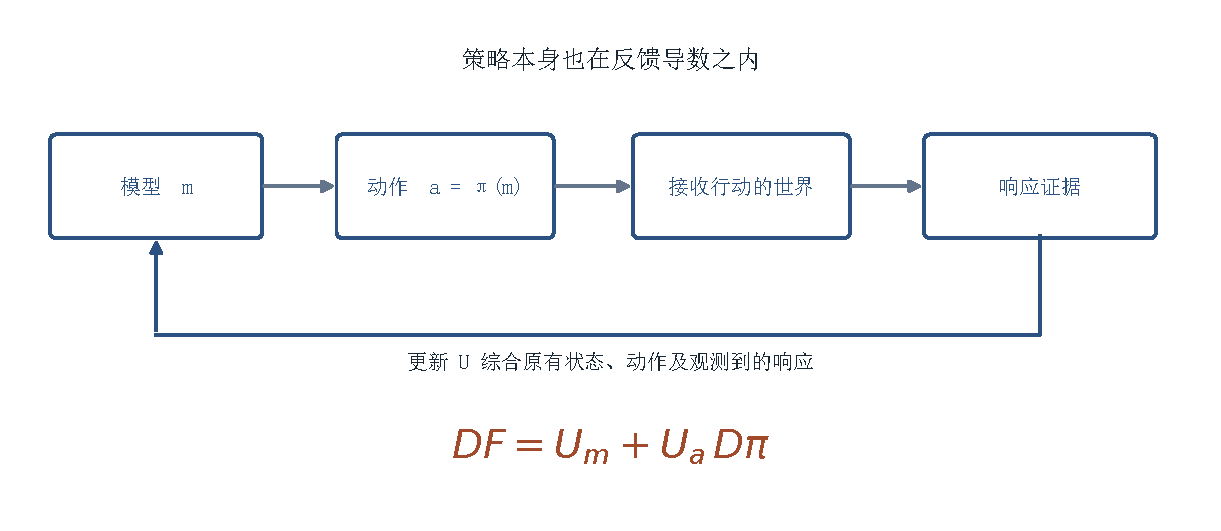
\includegraphics[width=\textwidth]{figures/model-action-loop.pdf}
\caption{模型通过策略改变动作，动作又改变下一次更新的证据。$U$综合保留状态、动作与环境响应，复合映射的导数同时包含直接项与经由策略的间接项。}
\label{fig:mechanism-model-action-loop}
\end{figure}
\furtherreading{%
W. Brian Arthur，\textit{The Nature of Technology: What It Is and How It Evolves}\\
Thomas P. Hughes，\textit{Rescuing Prometheus: Four Monumental Projects That Changed the Modern World}\\
Per Bak，\textit{How Nature Works: The Science of Self-Organized Criticality}\\
Sidney Dekker，\textit{Drift into Failure: From Hunting Broken Components to Understanding Complex Systems}\\
Stewart Brand，\textit{How Buildings Learn: What Happens After They’re Built}\\
Andy Clark，\textit{Surfing Uncertainty: Prediction, Action, and the Embodied Mind}\\
Sebastian Thrun, Wolfram Burgard and Dieter Fox，\textit{Probabilistic Robotics}\\
Judea Pearl and Dana Mackenzie，\textit{The Book of Why: The New Science of Cause and Effect}}


% <<<<<<<<<< parts/book-ch03.tex <<<<<<<<<<


% >>>>>>>>>> parts/book-ch04.tex >>>>>>>>>>
%% ===================== 本章参考文献 =====================
\printbibliography[heading=subbibliography,title=参考文献]

\chapter{生命、身体与位移：智能的模态分化}

第三章的收束指向一套更古老的压缩机制：它不靠传感器和反射，而靠世代更替记录哪些变量不能删去，靠繁殖失败来确认哪些压缩是错的。这套机制运行的介质，与位移系统有着根本不同的响应方式。对一段道路施加作用，返回的是摩擦、惯性和排队；对一个生命系统施加作用，返回的是代谢、修复、免疫、代偿和记忆。差别不只是反应快慢。位移系统的参数可以在设计阶段被标定，生命系统的响应会在干预之后继续演化，把设计阶段看不见的后果推迟到时间深处。一旦承认介质会解释作用，“智能应当收敛成什么形态”就不再是一个可以由单轴想象回答的问题。

\section{生命不是软件：基因代码的物理意义}

\subsection{代码隐喻的失效与超具身的信息结构}

介质有响应，这一点在生命系统上表现得最彻底：作用进入之后，会被系统本身重新解释。改变一个系统之前，需要先知道它是什么。位移系统可以按照质量、能量和拓扑来拆解，因为它的部件是外在地连接起来的：发动机、道路、空域、规章，各自可以被单独描述和替换。生命系统不是这样组织的。它的部件在物质上相互嵌入，它的结构由环境在漫长时间里选择并压缩出来。对这样的对象，最方便的描述方式往往也是最容易出错的方式。

\subhead{代码隐喻与物理执行}

把基因比作代码，是一个有用但危险的隐喻。它有用，是因为 DNA 的确具有信息性。碱基序列可以复制，可以突变，可以被读取，可以影响蛋白质合成，也可以在代际之间传递。没有这种信息结构，生命无法保持连续性，演化也无从积累。但它危险，是因为人们很容易进一步误以为：既然基因像代码，那么生命就像软件；既然软件可以编辑、调试、重构，那么生命也可以被同样方式重写。

这个推论忽略了生命系统最根本的事实：基因不是脱离硬件运行的程序。基因的意义不是只由 ATCG 的符号排列决定，而是由它在细胞物理化学环境中的执行方式决定。DNA 序列必须进入细胞核、染色质结构、转录调控、RNA 加工、蛋白质翻译、折叠、修饰、运输、降解、代谢状态、细胞类型、发育阶段和外部环境共同构成的系统，才会表现出功能。\key{基因不是写在身体里的软件，而是身体本身的一部分。}它的意义不是被读取出来的，而是在细胞环境中被物理执行出来的。

软件代码的意义通常由形式规则决定。一个函数在给定编程语言、编译器和运行环境中，有相对明确的输入输出关系。即使现实软件工程也充满依赖、兼容、接口和遗留问题，代码意义至少可以在较大程度上通过符号结构和执行规则分析。但基因不同。基因没有独立于细胞环境的纯粹意义。一段序列在不同细胞中可能被沉默、激活、剪接、修饰或放大；同一蛋白在不同代谢状态、不同组织环境、不同发育阶段中可能产生不同后果。它不是单独运行的指令，而是嵌入网络中的物理触发条件。

因此，基因型到表现型不是线性翻译，而是多层反应网络。DNA 序列只是起点之一。它要经过染色质开放程度、转录因子结合、RNA 剪接、翻译效率、蛋白折叠、蛋白互作、细胞信号、代谢通量、力学环境和组织结构的连续过滤。所谓“一个基因导致一个性状”的说法，只在极少数简单场景中近似成立\cite{manolio2009finding}。多数生命现象不是单基因指令的输出，而是网络状态的结果。基因提供可能性，细胞环境决定其实现方式，整个身体和外部环境则进一步改变其后果。

这也是为什么基因的物理实现不能被跳过。一个碱基突变不是抽象字符替换，而可能改变分子形状、结合能、折叠路径、反应速率、稳定性、空间构型和调控关系。结合能的变化不是修辞，它可以被写成一个具体的量：
\begin{equation}
\Delta\Delta G=RT\ln\frac{K_{\text{d}}^{\text{mut}}}{K_{\text{d}}^{\text{wt}}}
\label{eq:ch27-ddG}
\end{equation}
$\Delta\Delta G$采用“突变体减去野生型”的结合自由能约定，$K_{\mathrm d}$是对应解离常数。比值无量纲。突变体的$K_{\mathrm d}$增大十倍时，结合变弱，自由能差为正；在310开尔文下约为$5.9\,\mathrm{kJ/mol}$。它说明一个局部序列变化可能显著改变亲和力，功能后果还要经过浓度、动力学、定位与网络状态。

生命中的“语义”不是词典意义，而是热力学和动力学意义。一个序列的功能，最终体现在它如何改变物质流、能量流、信号流和结构稳定性。基因不是命令一台机器执行动作，而是改变一个复杂物理化学系统中的局部边界条件。这使生命系统不同于普通符号系统。语言可以容忍大量歧义，因为解释者可以补足上下文；软件可以在严格环境中运行，因为规则被人设计为离散、明确、可追踪；生命则在连续、嘈杂、热扰动、强耦合的环境中运行。温度、pH 值、离子浓度、蛋白质构象、分子拥挤、膜结构、机械压力和随机涨落\cite{ellis2001macromolecular}，都可能影响同一个基因结构的实际后果。生命不是在干净的逻辑空间中执行代码，而是在温暖、潮湿、拥挤、噪声充满的物质环境中维持秩序。

\subhead{超具身的信息结构}

如果基因的意义由执行环境决定，那么执行环境本身就不是背景，而是被写进了序列里。更进一步说，生命具有一种\term{超具身}特性。普通具身智能是一个模型获得身体，然后通过传感器和执行器进入环境；生命则不是先有一个抽象模型，再把它装进身体。生命的信息结构本身，就是身体与环境长期交互后的沉积物。基因并不只是记录“如何制造一个身体”，它还压缩了数十亿年环境选择留下的痕迹：哪些分子结构能够稳定存在，哪些代谢路径能够持续供能，哪些感知与行动方式能够提高存活概率，哪些发育程序能够在特定温度、营养、重力、微生物、捕食者和繁殖压力下保持可行。基因不是脱离环境的蓝图，而是环境长期刻进生命内部的历史。

因此，基因信息不是普通意义上的符号信息，而是经过自然选择筛选过的交互信息。它包含的不是完整世界模型，而是生命在特定物理世界中反复试错后留下的可生存结构。眼睛不是单纯由“造眼代码”生成的器官，而是光、介质、神经、运动、捕食和逃避共同塑形的结果；肺不是单纯由序列指定的部件，而是大气成分、代谢需求、体型结构和循环系统共同约束出来的结果；免疫系统也不是孤立程序，而是与病原体、共生菌、组织损伤和环境暴露长期博弈后的动态遗产。生命的“代码”从一开始就不是纯代码，而是环境压力、身体结构和历史选择共同压缩成的物质记忆。

这使基因编辑不同于软件修改。修改软件时，代码的运行环境大多由人设计并保持相对稳定；修改基因时，编辑的是一个已经把环境历史内化进自身结构的系统。一个序列片段之所以保留，可能不是因为它在当前单一指标下最优，而是因为它在漫长演化中与其他结构形成了隐性协同。它可能参与发育时序、代谢缓冲、免疫调节、组织稳定或压力响应。我们看到的是一段序列，实际触碰的是生命与环境长期耦合后的压缩层。这个压缩层越古老、越深，越不可能被简单还原为清晰的工程功能表。

\subsection{演化堆叠、通路式调控与四层纠缠}

\subhead{演化堆叠与拓扑刚性}

正因为生命具有这种超具身特性，生命系统也不是从零设计出来的。它是演化堆叠出来的。工程设计理想上可以从目标出发，选择干净结构，去除冗余，重构底层。生命不是这样来的。生命系统是长期演化中的历史沉积。一个结构只要在某个环境中足够可用，就可能被保留；一个原本用于某种功能的机制，可能被复用到另一种功能；一个局部补丁，可能在后来的演化中变成不可删除的基础接口；一个偶然形成的路径，可能因后来无数结构依赖它而变得不可替换。生命不是最优设计，而是可生存设计的累积。

这种演化堆叠导致生命系统中充满功能性遗留物。它们未必简洁，未必优雅，未必符合工程师的重构欲望，却可能被深深嵌入系统。一个看似冗余的通路，可能在压力环境下提供备用路径；一个看似低效的机制，可能承担调节、缓冲或发育时期的隐性功能；一个看似无关的片段，可能影响染色质结构、表达时序或远端调控。生命系统中的“废料”经常不是完全无用的垃圾，而是历史性结构的一部分。它可能没有单一清晰功能，却参与了系统的整体稳定。这就是生命拓扑刚性的来源之一。

生命不是由独立模块简单拼装而成，而是由长期依赖关系缠绕而成。一个局部修改可能牵动远端后果；一个短期有益的编辑可能改变长期发育；一个单点增强可能破坏代谢平衡；一个靶点抑制可能被旁路通路补偿；一个局部修复可能改变系统整体压力分布。生命系统的困难不只是“我们还不知道全部机制”，而是机制本身具有多层耦合、历史依赖和状态条件性。这种刚性不来自某个尚未解决的难点，而来自已知结构之间的依赖密度。但刚性不等于封闭，生命之所以可以被医学和生物技术改变，正是因为生命系统仍然存在通路。

\subhead{通路式调控与四层纠缠}

激素可以改变全身状态，神经递质可以改变行为倾向，受体可以放大或抑制信号，酶可以控制代谢通量，免疫检查点可以改变免疫反应，转录因子可以改变细胞命运，递送系统可以把干预送入特定组织。生命不是不可进入的黑箱，而是一个有入口、有杠杆、有脆弱点、有控制面的复杂网络。关键在于，这种操控不是软件式重写，而是通路式调控。药物不是直接改写身体的总体程序，而是通过受体、酶、离子通道、信号通路、免疫节点、代谢节点改变系统状态；基因编辑也不是任意重构生命，而是在特定细胞、特定时机、特定递送条件下改变局部结构。有效干预常常不是“全面重写”，而是找到一个足够关键、足够可达、足够低副作用的调控点，使系统从一个状态迁移到另一个状态。

通路的物理形式并不统一。小分子药物依赖受体口袋的形状匹配，抗体依赖表位的识别精度，基因编辑依赖递送载体在组织中的分布，细胞治疗依赖细胞进入体内之后的归巢与存活。通路的物质形式决定了干预的精度上限，也决定了同一套分子在不同个体身上能不能到达同一个位置。所谓“靶点”，因此不是分子上的一个位置，而是一条需要在体内走完的路径。

通路的容量与选择性是可以被量化的。腺相关病毒载体是目前基因治疗中使用最广的递送工具之一，其装载上限约为 4.7 千碱基，超过这一长度的编码序列无法被完整包装，而它在静脉给药后主要富集于肝脏，组织特异性因此成为载体工程最主要的改造目标。脂质纳米颗粒的载量更灵活，也可以重复给药，但它携带的编辑工具在体内只短暂表达，适合一次性完成编辑的场景，不适合需要长期补充基因产物的场景。递送方式决定了干预能到达哪些细胞、能持续多久、可以被重复多少次，这些限制并不来自编辑工具本身的精度\cite{naso2017adeno}。通路的物理形式因此划定的是干预效果的上限，而不只是实现细节。

因此，生命技术的真正难题不是“能不能操控”，而是“如何找到可承受的操控路径”。一个好的靶点必须同时满足多重条件：它在病理网络中足够关键，能被药物或编辑工具到达，改变后能产生稳定收益，副作用可以承受，长期反馈不会反噬，个体差异不会使风险失控。这个条件组非常严格。生命可被调控，但它要求干预者同时理解通路、网络、环境、时间和后果。

从技术黏滞的角度看，生命介质的高黏滞来自四层纠缠。第一层是物理化学纠缠。基因功能必须通过分子折叠、反应速率、结合能和空间构型实现。符号变化必须经过物质执行。第二层是网络纠缠。基因不是孤立指令，而是调控网络、代谢网络、信号网络和发育网络中的节点。局部变化会被系统放大、抵消或转移。

第三层是历史纠缠。生命系统不是重新设计出来的机器，而是演化堆叠出来的遗产。许多结构之所以存在，不是因为它们最优，而是因为它们在过去的约束下被保留，并被后来的结构继续依赖。第四层是通路约束。生命虽然可以被调控，但调控必须通过可达通路进入系统：递送路径、靶点特异性、剂量窗口、时序窗口、组织分布和反馈边界，都会决定干预能否真正生效。这四层纠缠共同说明：基因不是软件，生命不是干净的代码库，身体不是可随意替换的硬件平台。基因、身体、环境和历史在原子尺度上相互嵌入。所谓生命代码，只有在生命物质中才具有完整意义。

这并不否定基因技术的力量。相反，正因为基因技术可以触及生命系统的底层结构，它才具有很强的改变能力。但能力越大，越不能把生命简化为可编辑文本。真正成熟的生命技术，不是把身体当作低级硬件，而是承认基因意义的物理性、网络性、历史性和通路性。它不只是问“能不能编辑”，还要问“通过什么通路编辑、在哪个状态下编辑、会牵动哪些网络、长期由谁承担后果”。

基因不是软件。基因是被生命系统执行的物理结构，也是环境历史压缩后的物质记忆。生命可以被操控，但不能被任意重写。操控生命的关键，不是幻想改代码，而是在超具身的演化系统中寻找可承受的调控路径。

四层纠缠说明，干预必须落在通路上。但通路的存在只回答了问题的一半。一旦通路被使用，干预就进入了系统自身的运行过程：它会被代谢、被补偿、被修复、被免疫识别，也会在时间中展开出短期看不见的后果。一条在设计阶段可承受的调控路径，在系统作出回应之后是否仍然可承受，需要另一套分析。

\section{生命的剪切增稠：生物干预为什么越快越硬}

\subsection{响应系统与通路控制面}

可承受的调控路径在设计阶段成立，并不意味着它在被使用之后仍然成立。生命系统不是被动接受改变的材料，它对改变本身有回应。这个区别改变了干预问题的形式：外部作用的强度增加，不一定带来效果的增加。

\subhead{响应系统}

生命系统不是普通负载。对一块金属施力，它会变形、断裂或恢复；对一段代码修改，它会编译、报错或运行；但对一个生命系统干预，它会解释这种干预。它会代谢、免疫、修复、补偿、适应、记忆、反弹。生命不是被动承受外部作用的材料，而是具有自我维持倾向的动态系统。外部输入进入生命之后，不只是改变状态，也会触发系统对改变本身的回应。这就是生物干预的第一性困难：干预对象不是静态对象，而是响应系统。

但这并不意味着生命不可干预。医学、药物、疫苗、外科手术、激素治疗、免疫治疗、基因疗法和再生医学，都已经证明生命可以被深刻改变。生命系统有通路，有靶点，有窗口，有杠杆。关键不是“生命能不能被操控”，而是“操控以什么方式进入系统，是否被系统吸收，是否引发可承受的后果”。

许多技术想象默认，只要我们能找到足够精确的靶点，生命就可以像机器一样被调节。一个通路过强，就抑制它；一个蛋白缺失，就补上它；一个基因异常，就修复它；一个代谢指标不佳，就调回去。这个想法在某些场景中有效，但它低估了生命系统的网络性。生命系统并不总是接受单点改变。它可能绕开被抑制的通路，放大备用机制，改变受体敏感性，调节上游输入，转移代谢压力，或在长期内形成耐受和反弹。

因此，生命干预经常表现出非线性阻力。低强度、低频率、顺应系统节律的干预，可能被系统吸收；高强度、高频率、粗暴越过反馈周期的干预，可能让阻力急剧上升。这种非线性在流变学中有一个对应物。\term{剪切增稠}指颗粒悬浮液在剪切速率超过临界值之后黏度骤升的现象：低速剪切时，颗粒被流体隔开，悬浮液可以流动；剪切速率提高后，颗粒来不及彼此错开而被挤成密集排列，流体无法继续充当颗粒之间的润滑层，表观黏度在很窄的速率区间内上升若干数量级\cite{brown2014shear}。在一定范围内，这一行为可以用幂律描述：
\begin{equation}
\eta(\dot\gamma)=\eta_b+k\dot\gamma^{\,n}
\label{eq:ch28-thickening}
\end{equation}
这里$\eta$与$\eta_b$的单位为帕斯卡秒，$\dot\gamma$为每秒，$n$无量纲，因此$k$的单位为$\mathrm{Pa\,s^{n+1}}$。这个式子描述给定区间内的增稠分支；低速变稀、突变堵塞与完整流变曲线还需要其他机制和形式。

在这个表达式中，$k>0$、$n>0$使黏度随速率上升。平台项与幂律项相等的位置可以作为模型内的交叉尺度：
\begin{equation}
\dot\gamma_c=\left(\frac{\eta_b}{k}\right)^{1/n}
\label{eq:ch28-gamma-c}
\end{equation}
右式单位为每秒。这是由两项相等定义的交叉点，不自动等于实测增稠起点。用于生命干预时，还要分别定义强度、频率、持续时间与“阻力”的测量口径，确认是哪一种代偿、饱和或损伤机制产生了相似曲线。

对某一种具体干预，可以检验：增加强度或加快节奏以后，收益是否递减，补偿或副作用是否上升。剂量、频率和速度不是同一个变量；有些干预需要足够强或足够及时才有效。剪切增稠在这里提出一种响应假设，实际关系由对应机制和测量决定。

\subhead{通路与控制面}

既然阻力来自系统内部的反馈结构，干预落在哪个位置就成了决定性的变量。药物干预是最直接的例子。一个药物进入身体，不是只遇到一个靶点，而是进入吸收、分布、代谢、排泄、免疫、组织屏障、受体调节和个体差异构成的系统。短期指标改善，不等于长期系统改善；单点抑制有效，不等于整体风险下降；剂量增加不一定带来线性收益，可能带来毒性、副作用、耐受、反调节和系统性压力。生命系统不是一条直线，而是一张会变形的网。

不过，药物之所以能起作用，正是因为这张网并非均质。某些节点具有更强控制力。受体、酶、离子通道、转录因子、免疫检查点、激素轴、代谢瓶颈，都可能成为调控通路。医学进步的很大一部分，不是粗暴压制生命，而是在复杂网络中寻找可以被进入、可以被放大、可以被安全调节的关键节点。好的靶点不是单纯“重要”，而是同时可达、可调、可验证、可承受。

这使生命干预具有一种特殊形式：它不是直接控制整体，而是通过局部通道改变系统状态。一个有效药物并不需要理解身体的所有细节，正如一个舵不需要推动整艘船的每一块钢板。关键在于找到能改变方向的控制面。但生命系统的控制面并不稳定。它会随年龄、疾病阶段、遗传背景、组织环境、免疫状态和长期用药而变化。今天有效的通路，明天可能被代偿；一个人有效的靶点，在另一个人身上可能副作用更大。

基因编辑同样如此。编辑工具可以越来越精确，但生命对编辑的响应仍然复杂。一个局部序列被改变之后，它的后果要经过表达、折叠、调控、细胞环境、发育状态和长期反馈。编辑不是结束，而是开始。生命系统会把编辑结果放入自身运行网络中重新解释。短期看似正确的修改，可能在不同组织、不同年龄、不同遗传背景或不同环境压力下显露新的后果。

所以，基因编辑的难点不只是切得准，还包括送得到、改得对、表达稳、反馈可控、长期安全。递送系统、组织特异性、编辑效率、脱靶效应、免疫反应、细胞选择压力和发育时序，都是干预通路的一部分。生命技术越深入底层，越不能只把问题看成“编辑精度”，而要看作“通路设计”。

免疫系统更能说明这种剪切增稠。免疫不是简单防御机制，而是一个高度敏感的识别和调节系统。过弱会失守，过强会自伤；过慢会被感染压倒，过快可能引发炎症风暴\cite{fajgenbaum2020cytokinestorm}。外部干预如果没有匹配免疫系统的时序和强度，就可能从治疗变成扰动。生命系统最难的地方，不是它不反应，而是它反应太多、太复杂、太依赖时机。

这也是为什么生物技术不能直接复制软件迭代逻辑。软件可以高频发布、回滚、灰度测试、快速修补；生命干预不能随意在人身上高频试错。软件错误多数停留在信息系统内部，生命错误会进入身体、组织、代谢和长期风险。一次错误干预可能改变不可逆发育过程，可能留下长期损伤，可能通过免疫记忆、细胞状态或生态关系延迟显现。生命系统不允许无限次低成本回滚。

\subsection{黏滞来源、鲁棒性代价与在线维护的极限}

\subhead{黏滞来源与鲁棒性代价}

从技术黏滞的角度看，生命的剪切增稠来自三个来源。第一是时间刚性。生命反馈需要时间。药效需要时间展开，副作用需要时间观察，免疫反应需要时间发展，组织修复需要时间完成，发育和衰老更是在长周期中显现。外部干预如果只看短期响应，就容易把尚未返回的长期反馈误认为不存在。生命常把代价藏在时间里。

第二是结构耦合。生命系统的通路不是孤立管道，而是互相连接、互相补偿、互相限制的网络。单点改变可能通过网络传导到远端，局部收益可能伴随全局代价。系统越复杂，越不能把一个指标的改善直接等同于生命状态的改善。

第三是维护压力。生命是远离平衡态的耗散结构，必须持续输入能量、修复损伤、排除废物、维持边界和调节内部状态。生命不能像机器一样停机维护。心脏、免疫、神经、代谢、内分泌、细胞修复都必须在运行中完成。所有修复都发生在系统仍然承载功能的时候。这使干预强度和精度都受到限制：太弱没有效果，太强扰乱运行；太快越过反馈，太慢错过窗口。

这也可以帮助理解新药研发效率困境。现代生物技术、自动化实验和 AI 可以显著扩大候选空间。靶点可以更快发现，分子可以更快生成，结构可以更快预测，实验可以更快筛选。但发现端加速之后，瓶颈并不会自动消失，而是转向生命系统本身的验证、代偿和长期安全性。候选越多，验证越重；靶点越精确，系统反馈越需要理解；早期发现越快，后期临床失败的代价越高。所谓 Eroom 现象\cite{scannell2012diagnosing}，不能被简单归结为某一个因素，但它提醒我们：生物发现工具的进步，并不自动穿透生命系统的高黏滞验证层。

药物研发中的时间和费用随疾病、试验设计、失败分摊与资本口径变化。2016年的一项公司样本研究提供过较高的资本化成本估计，它不是每款新药的固定价格。\cite{dimasi2016} 更新的观察点是rentosertib：企业在2026年9月宣布三期项目首位患者给药。\cite{insilico2026phase3} 到达这个阶段构成进展，三期结果仍须通过后续观察建立。

发现端与验证端之间的落差可以用在制品数量来称量，

\begin{equation}
L=\lambda W
\end{equation}

$L$为稳定流程内的平均在制品数，$\lambda$为同一边界的平均通过率，$W$为平均停留时间。这是Little关系，退出、撤回和早期失败都要按一致口径计入。提高到达率、扩容、改善选择和改变停留时间，会共同影响库存与产出。若到达率持续超过服务能力，队列不断增长，就不能直接用稳态平均式解释全过程。

三个来源之外，生命还有一项与它们方向相反的性质。生命的鲁棒性是双刃剑。它让身体能够抵抗扰动、修复损伤、维持稳定，也让外部干预难以线性生效。一个脆弱系统容易被改变，也容易崩溃；一个鲁棒系统能够存活，也更会抵抗改变。生命之所以难治，正因为生命仍在努力维持自己。疾病不是一个独立敌人，而常常是身体网络在特定历史、遗传、环境和行为条件下形成的状态。治疗不是删除错误，而是推动整个系统从一个稳定状态迁移到另一个稳定状态。

但这种迁移不是盲目的。系统医学、网络药理学、精准医疗和合成生物学的价值，就在于它们试图识别状态迁移的通路。它们不是把生命当作不可知的神秘整体，而是承认生命有结构、有节点、有控制面，只是这些控制面嵌在反馈网络和时间过程之中。真正有效的生物干预，往往不是最大力度的干预，而是最适合系统状态的干预：在正确靶点、正确剂量、正确时序、正确人群和正确验证框架中，推动系统越过某个病理稳定态。

这使“越快越好”的技术直觉在生命领域经常失效。干预速度过快，可能越过系统弛豫时间；指标调整过猛，可能触发反调节；局部控制越强，越可能把压力转移到别处；候选生成越多，越可能堆积在验证瓶颈前。生命系统不是拒绝技术，而是要求技术进入它的节律。好的生物技术不是把生命当作慢软件，而是理解生命的反馈、冗余、代偿、时序和不可逆性。到这里，剪切增稠还只是一个横截面上的判断，它在时间维度上的极限形态还没有被处理。
\begin{figure}[ht]
\centering
% >>>>>>>>>> figs/fig-shear-thickening.tex >>>>>>>>>>
% 图 28-1  剪切增稠：低速率省力，高速率反噬
% (a) 线性坐标三段形态（定性）；(b) 双对数三段斜率：-0.45 / 0 / +2
%     (b) 中两轴同尺度（1 个十倍程 = 1.10 cm），故视觉斜率=数值斜率：
%     变稀段 Δlogη/Δlogγ̇ = -0.675/1.5 = -0.45；增稠段 = 1.8/0.9 = +2
\begin{tikzpicture}[x=1cm, y=1cm, font=\small,
  ax/.style={-{Stealth[length=2.0mm]}, ink, line width=0.6pt},
  tick/.style={anchor=north, font=\scriptsize, text=slate},
  ytick/.style={anchor=east, font=\scriptsize, text=slate},
  zone/.style={anchor=center, font=\scriptsize\heiti},
  slope/.style={font=\scriptsize, text=ink}
]
% 下边原来切掉约 2.5pt：底部 (a)/(b) 小标题贴下缘。放 0.18cm。（用 _figclip.py 量出）
% 左缘原先 0.50，纵轴符号 $\eta$ 距页边只剩 1.09pt；下缘 -6.64 处小标题余约 2.3pt。
% 两条边各放宽一点：左 0.50→0.28，下 -6.64→-6.85。
\useasboundingbox (0.28,-0.62) rectangle (14.06,-6.85);

\def\ax{0.95} \def\ay{-5.60} \def\aw{5.20} \def\ah{4.20}

% ================= (a) 线性坐标：三段形态 =================
% 公式放在图上方空白处，不压曲线
\node[font=\small, text=ink, anchor=center] at (3.55,-0.95)
      {$\eta(\dot\gamma)=\eta_0+k\,\dot\gamma^{\,n}$};

\draw[ax] (\ax,\ay) -- ({\ax+\aw+0.40},\ay)
      node[anchor=west, font=\scriptsize, text=ink] {剪切速率 $\dot\gamma$};
\draw[ax] (\ax,\ay) -- (\ax,{\ay+\ah+0.15})
      node[anchor=south, font=\scriptsize, text=ink] {黏度 $\eta$};

% 三段形态（定性）
\draw[ink, line width=1.3pt]
      (\ax,-1.988)
      .. controls (1.55,-3.35) and (2.45,-4.088) .. (3.03,-4.088)
      -- (4.59,-4.088)
      .. controls (5.25,-4.088) and (5.75,-2.60) .. (6.15,-1.652);
% η0 参考线与平台
\draw[slate!55, line width=0.4pt, dashed] (\ax,-4.088) -- (2.95,-4.088);
\node[ytick] at (0.90,-4.088) {$\eta_0$};
% 临界速率
\draw[slate!55, line width=0.4pt, dashed] (4.59,-4.088) -- (4.59,\ay);
\node[font=\scriptsize, text=ink, anchor=north] at (4.59,-5.72) {$\dot\gamma_c$};
% 三段分区与短签
\draw[slate!35, line width=0.4pt, dashed] (3.03,\ay) -- (3.03,-4.85);
\node[zone, text=deepblue!90] at (1.99,-4.60) {变稀};
\node[zone, text=terra!90]    at (3.81,-4.60) {牛顿平台};
\node[zone, text=rust!90]     at (5.37,-4.60) {增稠};

% ================= (b) 双对数坐标：三段斜率 =================
\def\lox{8.75} \def\loy{-5.60}
\def\dc{1.10}            % 1 个十倍程
% 坐标轴
\draw[ax] (\lox,\loy) -- ({\lox+\dc*4+0.35},\loy)
      node[anchor=west, font=\scriptsize, text=ink] {$\dot\gamma$};
\draw[ax] (\lox,\loy) -- (\lox,{\loy+\dc*3+0.10})
      node[anchor=south, font=\scriptsize, text=ink] {$\eta$};
\foreach \e in {0,...,4} {
  \pgfmathsetmacro\xx{\lox+\dc*\e}
  \draw[slate!55, line width=0.4pt] (\xx,\loy) -- (\xx,\loy-0.08);
  \node[tick] at (\xx,\loy-0.10) {$10^{\e}$};
}
\foreach \e in {0,...,3} {
  \pgfmathsetmacro\yy{\loy+\dc*\e}
  \draw[slate!55, line width=0.4pt] (\lox,\yy) -- (\lox-0.08,\yy);
  \node[ytick] at (\lox-0.10,\yy) {$10^{\e}$};
}
% 三段直线：同尺度下视觉斜率=数值斜率
\draw[deepblue!85, line width=1.4pt] (\lox,{\loy+\dc*1.675}) -- ({\lox+\dc*1.5},{\loy+\dc});
\draw[terra!90,    line width=1.4pt] ({\lox+\dc*1.5},{\loy+\dc}) -- ({\lox+\dc*2.5},{\loy+\dc});
\draw[rust!90,     line width=1.4pt] ({\lox+\dc*2.5},{\loy+\dc}) -- ({\lox+\dc*3.4},{\loy+\dc*2.8});
% 拐点
\draw[slate!55, line width=0.4pt, dashed] ({\lox+\dc*2.5},\loy) -- ({\lox+\dc*2.5},{\loy+\dc});
\node[font=\scriptsize, text=ink, anchor=north] at ({\lox+\dc*2.5},-5.72) {$\dot\gamma_c$};
% 每段旁各标一个公式片段（离线留白，不压线）
\node[slope, text=deepblue!85, anchor=south west] at (8.82,-3.58)
      {$\eta\propto\dot\gamma^{-0.45}$};
\node[slope, text=terra!90, anchor=south west] at (10.50,-4.32)
      {$\eta\approx\eta_0$};
\node[slope, text=rust!90, anchor=south east] at (12.35,-2.64)
      {$\eta\propto\dot\gamma^{2}$};

% ================= 栏标题（一律在内容下方）=================
\node[anchor=north, font=\footnotesize\heiti, text=slate] at (3.55,-6.22) {(a) 三段形态};
\node[anchor=north, font=\footnotesize\heiti, text=slate] at (10.95,-6.22) {(b) 双对数斜率};
\end{tikzpicture}

% <<<<<<<<<< figs/fig-shear-thickening.tex <<<<<<<<<<

\caption{剪切增稠：低速率省力，高速率反噬。(a) 三段形态；(b) 双对数坐标下的三段斜率为 $-0.45$、$0$、$+2$，两轴同尺度，因此视觉斜率等于数值斜率。对生命系统的干预速率越高，系统的补偿性反应越强，有效黏滞不降反升。}
\label{fig:shear-thickening}
\end{figure}


\subhead{在线维护的极限与干预节律}

衰老可以看作在线维护的极限。生命体从出生开始就在持续修复自身：DNA 损伤修复、蛋白质质量控制、细胞更新、免疫清除、代谢调节、组织再生。但修复并不完美。损伤会积累，错误会残留，冗余会消耗，调节网络会变钝，系统会逐渐失去弹性。衰老不是单一部件损坏，而是长期运行系统中维护压力、信息噪声、结构损伤和反馈失调的共同结果\cite{lopezotin2013hallmarks}。

死亡则显示了个体在线维护的边界。对个体而言，死亡是终止；但从种群和演化角度看，代际更替提供了一种更新机制。它让生命不必无限修补同一个个体，而是通过繁殖、变异、选择和重组，让系统在更高层级上继续搜索。这个说法不是为死亡赋予浪漫意义，也不是说死亡对个体是好事，而是指出：生命无法无限在线维护，种群层面的更新部分承担了个体层面无法解决的累积损伤和结构僵化。

这也解释了生命介质为什么具有特殊黏滞。它既有比特属性，因为基因可复制、可传递、可编辑；又有原子属性，因为基因必须在物理化学环境中执行；还有生命属性，因为执行结果会进入反馈、代偿、修复和演化。它不是轻介质，而是比特、原子与生命的重叠区。AI 可以加速其中的信息搜索，却不能取消其中的物理执行、时间展开和系统响应。

成熟的生命技术，不能只追求更强编辑、更快筛选、更大模型。它还必须学会寻找通路、匹配时序、控制剂量、分层验证、缓冲风险和尊重反馈。某些场景适合强干预，某些场景只能温和调节；某些目标可以快速验证，某些后果必须长期观察；某些残差可以交给模型吸收，某些残差必须交给临床、制度和伦理边界承担。

生命不是软件，也不是普通机器。它是会维护自身、解释干预、抵抗扰动、延迟反馈的耗散结构。生物干预的难点，不在于生命不可改变。生命当然可以被改变。难点在于：真正有效的改变必须找到通路、穿过反馈、尊重节律，并承受长期验证。\key{推得越快，系统未必越顺，反而可能越硬。}这就是生命的剪切增稠。

剪切增稠把代价重新推回承受者一侧。无论干预设计得多么精确，扰动、代偿、不可逆后果和长期验证都必须落在某个仍然在运行的系统上。承受有边界，也有时限：能吸收的扰动、能推迟的反馈、能承担的不可逆改变都是有限的。什么可以被承受、由谁承受、承受多久，构成的问题比干预技术本身更基础。

\section{形态计算之后：身体封装与演化摊销}

\subsection{物理智能的残差问题与身体封装的三层结构}

承受总要落在某个具体结构上。生命把大量残差修正压进了演化、发育和环境的共适配，机器没有这套结构，它在物理世界中的每一次行动，都要靠显式工程结构来吸收偏差。第三章留下的压缩判据决定了模型保留哪些变量，但这些变量在物理接触中由谁修正、以多大延迟修正、失败之后能否恢复，并不是模型内部可以回答的问题。

物理智能最容易被误解的一点，是把身体看成智能的外设。在这种理解里，真正的智能位于大脑、模型或控制系统之中，身体只是执行命令的机械端口，系统先理解世界，再规划动作，最后由身体把计划落实到现实；按照这种图式，只要模型足够强、传感器足够多、控制足够精细，机器就应当能够像人一样进入现实世界。但物理智能的真实困难，不在于生成一个动作，而在于在开放现实中连续行动，而连续行动要先承认一件模型不愿承认的事：现实会持续产生模型没有预写的偏差。

\subhead{物理智能的残差问题}

现实不是等待执行的静态对象，而是一个不断产生残差的开放系统。模型可以给出动作，现实会给出偏差。地面可能比预期更滑，物体可能比视觉判断更重，杯壁可能有水，门把手可能松动，人的身体可能突然失衡，光线可能变化，传感器可能被遮挡，执行器可能存在延迟。每一个偏差单独看都很小，但物理任务不是一次问答，而是一条任务链：一次小的识别误差会改变抓取姿态，一次小的接触偏差会改变物体位置，一次定位漂移会进入下一轮规划，一次反馈延迟会放大控制误差，残差不会在动作之间自动清零，而会沿着任务链传播。

这里所说的\term{残差}，不是一个单一误差项，而是开放物理行动中未被当前模型、身体、控制器或运行体系完全吸收的偏差总称，它至少包括四类：模型残差，即世界模型或策略模型压缩后遗漏的状态变量；感知残差，即传感器噪声、遮挡、漂移和多模态不同步造成的状态估计偏差；接触残差，即摩擦、滑移、变形、冲击和力传递中的不可完全预测部分；运行残差，即异常处理、维护、验证、接管和责任追溯中的系统性负担。要紧的不是这些残差是否存在，它们在开放行动中总是存在，而是在连续任务链中它们是否会被及时吸收，还是沿接口传播并越过可恢复边界。因此，具身智能真正要解决的，不是能不能做某个动作，而是能不能在连续任务中把残差压在可恢复范围内。

抓杯子只是最小例子。现实中的机器人面对的是清洁房间、护理老人、整理桌面、搬运货物、工地协作、农田采摘、医院送药，每个任务都由许多动作串联而成，每个动作又改变下一个动作的初始条件，系统真正要证明的，不是它能不能成功一次，而是它能不能在长时间、多扰动、高责任的任务链中保持可恢复性。这里的困难有明确的门槛形状：超过某个残差阈值，能力不是平滑下降，而可能突然表现为停机、误抓、碰撞、失衡或请求人工接管。于是问题就落到承载残差的结构上，而人类身体的特殊之处，不是拥有完整世界模型，而是把大量残差修正压进了身体、经验和环境共适配之中。

\subhead{身体封装的三层结构}

拿起一个杯子时，人不会先计算杯子的精确几何、摩擦系数、重心位置、表面湿度、接触角度和力分布，人只是看一眼，伸手，触碰。手指立刻感到滑不滑，肌肉立刻感到重不重，关节立刻修正姿态，杯子一有微小滑移，指腹和肌肉就自动调整夹持力度。很多误差还没有进入意识，就已经被身体吸收，这就是\term{身体封装}。\key{身体不是智能的外设，而是残差管理系统。}它把开放现实中的大量偏差压缩在低延迟、连续反馈、自修正的闭环里。

身体封装不是说身体“很重要”这么简单，而是说身体本身是一套残差吸收结构。皮肤、肌肉、肌腱、关节、骨骼、前庭系统、本体感觉、痛觉和反射，并不是大脑之外的附属装置，而是感知、执行、缓冲、约束和修正的连续系统：手指柔软，会自动适配物体表面；肌肉有弹性，会吸收冲击；关节有限位，会限制危险动作；痛觉会标记过载；经验会提示哪些细节可以忽略，哪些细节意味着危险。身体不是把所有信息传给大脑再等待计算，而是在接触中直接处理一部分现实。

身体之所以能够封装残差，并不是因为它绕开了物理规律，而是因为它把一部分物理规律变成了行动结构。摆腿时的重力势能与动能转换、肌肉与肌腱中的弹性储能、指腹接触时的局部形变、关节限位对危险姿态的排除，都不是中央控制器事后补偿出来的结果，而是身体形态预先把某些误差限制在可承接的动力学通道中；成熟身体不是每一刻都用主动控制对抗重力、惯性、摩擦和接触，而是在许多场景中让这些物理关系先完成一部分约束、筛选和修正。由此看，形态计算的深层意义不只是“身体参与计算”，而是身体把一部分原本需要感知、估计和控制的残差，转化为材料、几何和被动动力学中的低成本约束\cite{paul2006}，被动动力行走机器人正是这条思路的直接证据：在恰当形态和动力学条件下，稳定运动并不必然依赖高强度中央控制，身体结构本身可以承担一部分运动组织\cite{mcgeer1990,full1999,collins2005}。

封装至少发生在三层。第一层是材料封装，皮肤、肌肉、肌腱和关节以物理方式吸收误差，柔软的指腹扩大接触面积，肌肉弹性缓冲冲击，步态中的身体弹性帮助稳定行走，这里的“计算”不是符号计算，而是材料和形态直接参与控制，形态计算研究之所以重要，正在于它把身体形状、材料顺应性、被动动力学和环境耦合纳入控制问题，一部分本来需要中央控制器处理的复杂性，可以由身体结构本身分担\cite{paul2006}。第二层是反馈封装，人通过视觉、触觉、本体感觉、前庭系统和肌肉张力，在行动中连续采样现实：地面是否湿滑，脚底一压就知道；物体是否松动，手指一碰就知道；对方身体是否失衡，手臂一接触就会调整，世界不需要被完整预装，而可以在行动中被局部询问，阻抗控制在机器人操作中成为基础概念，正是因为接触任务不能被还原为纯位置跟踪，操作者、执行器、物体和环境构成同一个动力学耦合系统，控制的对象不是孤立轨迹，而是交互关系\cite{hogan1985}。第三层是经验封装，人见过无数杯子、门把手、楼梯、湿地面、刀具、热锅、疲惫的人体和拥挤的空间，这些经验不是完整模型，而是大量可行动的有损压缩，人知道哪些细节通常可以忽略，哪些细节必须立即处理，身体让模型可以不完整，经验让行动可以不从零开始\cite{gibson1979}。

这一路径与 Moravec 悖论、具身认知和形态计算传统相通\cite{moravec1988,pfeifer2007,varela1991,gibsonpick2000,pfeiferbongard2006,hauser2011}。Moravec 悖论提示，对机器来说，抽象推理未必最难，反而是人类幼儿即可完成的感知-运动能力极难工程化；具身认知指出，智能不只存在于头脑中，而是在身体、环境和行动之间形成；形态计算进一步强调，身体材料与形态可以参与控制。本节要推进的是其中一层更具体的判断：身体封装的不是抽象计算量，而是残差的低延迟吸收能力。不过，这个判断很容易被读成身体天然优于机器，而原文自身也留下了修正条款：人类并不是只把复杂性内化，机器也不是只能把复杂性外化，人类把一部分残差交给环境，门把手、楼梯、桌椅、道路和工具，都是围绕人体尺度形成的外部封装，机器也可以把一部分残差压回身体，柔性夹爪、弹性关节、机械限位和顺应性材料，都是机器的内部封装。真正的差异不在于人内化、机器外化，而在于时间分母与基质可供性这两条更底层的轴，这一点留到本节最后一个小节处理；眼下要先回答的是另一个问题：既然机器也有办法修正残差，为什么它仍然显得沉重？

\subsection{机器复杂度展现与接口债务}

\subhead{机器复杂度展现与接口债务}

机器并不是没有办法修正残差，而且路径很多。它可以通过传感器展现残差，摄像头、深度相机、激光雷达、触觉、力矩、IMU、本体感觉，都可以让机器知道自己偏了多少、滑了没有、撞了没有、姿态漂了没有；可以通过控制算法修正残差，闭环控制、阻抗控制、模型预测控制、实时重规划，可以把小误差不断拉回轨道；可以通过身体结构吸收残差，柔性夹爪、欠驱动手、弹性关节、顺应性材料、机械限位、被动稳定结构，都可以让身体自己消化一部分误差\cite{mason1985,birglen2008}；可以通过更强模型预测残差，视觉-语言-动作模型、世界模型、模仿学习和策略模型，可以从较少输入中推断更多状态，提前避开危险动作\cite{shao2025,li2025}；可以通过环境改造减少残差，标准货架、二维码、专用夹具、固定路线、封闭园区、轨道系统、V2X、结构化仓库，都是让环境替机器降低开放性；还可以通过任务收缩和运行体系限制残差，扫地、仓储搬运、巡检、手术辅助、焊接、采摘、配送各自收缩任务边界，远程接管、安全员、异常工单、日志审计、维护人员和保险责任，则把残差转入更大的运行结构。真正的问题不在于办法够不够多，而在于人类把大量残差修正沉入身体、经验和环境，机器往往必须把残差修正展现为工程系统。

这就是\term{机器复杂度展现}。所谓复杂度展现，不是简单地“机器需要更多传感器”，也不是“机器硬件不如人”，它指的是：在人类身体中被连续、局部、低延迟处理的现实复杂性，在机器那里必须被拆成可测量、可同步、可控制、可验证、可维护、可追责的工程结构。人用手指感知滑移，机器可能需要触觉传感器、滑移检测算法、控制反馈和安全策略；人用肌肉缓冲碰撞，机器可能需要柔顺材料、力控策略和机械保护；人通过经验理解“轻一点”“别弄坏”“扶稳一点”，机器必须把这些模糊约束转化为动作规则、风险边界和责任记录。身体里原本连在一起的东西，被机器拆成了模块，模块一多，接口就出现，接口一多，残差传播路径就增加。

这可以称为\term{接口债务}：当隐含在身体闭环中的残差修正被拆成多个工程模块后，系统必须持续承担同步、标定、延迟补偿、故障传播、维护和验证的结构性负担。在人类身体中，感知、执行、缓冲、修正和安全边界不是五个独立系统，手指触到杯壁的瞬间，触觉、肌肉张力、关节角度、皮肤形变和经验判断已经在同一个身体闭环中完成局部修正，变量没有被完全命名，误差没有被完全展开，控制也没有被拆成彼此独立的模块；机器不同，滑移要被检测，触觉要被标定，视觉要和力觉同步，控制器要补偿延迟，执行器要承接误差，安全系统要判断边界，日志系统要记录行为，验证系统要证明可靠，责任系统要追溯后果。每拆出一个变量，就多一个接口，每多一个接口，就多一个同步问题、故障模式和维护点。若把模块间的耦合近似为两两都可能相关，接口数量的增长可以写成
\begin{equation}
N_{\text{if}}=\frac{n(n-1)}{2}
\end{equation}
其中 $n$ 是被显式拆分的模块数，$N_{\text{if}}$ 是系统需要维护的成对接口数，两者都是无量纲计数，系数 $1/2$ 来自成对通道无序，一条通道不重复计数。在每一对模块之间至少需要一条同步、标定或误差传递通道的假设下，这个式子给出的是接口数量的上限而非实计数：$n$ 从五增到十，上限从十增到四十五，增长快于模块数本身。真实系统的依赖通常不是全连接，很多成对通道并不活跃，实际接口数低于该上限，但方向不变，模块拆得越细，需要同步、标定和验证的关系增长得越快。展现因此不是把复杂性看清楚这么简单，而是把隐含复杂性转化为显式耦合结构。

接口债务也不是普通的集成成本。普通集成成本强调模块多了会麻烦，接口债务强调残差会沿接口传播：感知偏差会进入控制，控制偏差会进入执行，执行偏差会改变环境，环境变化又反过来污染下一次感知；模块越多，残差传播路径越多，任务链越长，残差越容易从局部误差变成系统偏移，机器的沉重不来自某一个部件，而来自这些显式结构之间不断累积的耦合债务。这里面还藏着一层更隐蔽的时间债务：机器系统中的视觉、触觉、力矩、本体感觉、规划器和执行器通常具有不同的采样率、延迟和相位，每个模块都在处理某个时间片上的世界，但这些时间片并不天然重合，控制器拿到的“当前状态”，往往已经是多路异步信号经过时间戳、滤波、外推和融合之后生成的工程对象。只要任务进入高速接触或连续操作，残差就不只是从一个模块传到另一个模块，还会从一个时间相位错位到另一个时间相位，系统修正的可能不是此刻的误差，而是刚刚过去的误差，下一次动作又会把这个滞后的修正写入新的物理状态；于是接口越多，系统不仅越难集成，也越难维持一个稳定、共同、可行动的“现在”。身体的接缝不需要被逐一命名，机器的接缝必须被逐一维护。

反过来看，“展现”也不等于“堆料”。成熟工程不一定是把所有东西做得更通用、更复杂，一个柔性夹爪可能比高精度机械手加复杂触觉阵列更适合抓软物体，一个固定工装可能比通用识别模型更可靠，一个机械限位可能比复杂软件安全策略更稳定，一个封闭园区可能比开放道路更容易自动驾驶，真正的问题不是传感器够不够多，而是残差由谁修正、在哪里修正、以什么物理和工程代价修正。软体机器人和欠驱动结构正是在这个方向上展开，它们不是简单模仿生物外形，而是试图让材料顺应性、接触几何和被动形变参与控制，使机器人不必把每一次接触都转化为高精度测量和中央计算；Rus 和 Tolley 的综述指出，柔性材料使机器人能够走出刚性机器人的设计、制造和控制路线，但软体结构也带来建模、感知、驱动和控制的新困难\cite{rus2015}。这说明身体可以吸收残差，但身体本身也会引入新的显式复杂性，它不是免费解法，而是另一种复杂性分配方式。既然复杂性总要被分配，把其中一部分交给更强的模型，就成了下一条看似最直接的出路。

\subsection{预测不能取消承受：任务链与断崖式失效}

\subhead{预测不能取消承受}

模型可以减少误差、避免危险接触，也能让现有硬件完成更多任务。物理闭环还需要足够的力、速度、感知与恢复能力：滑移发生以后，要有接触与控制结构接住；部件损坏以后，要有修复或替代路径。预测、执行和恢复的能力，应分别检查。

这并不是否认大脑的价值。更强的视觉模型、世界模型、动作模型和策略学习，确实可以让已有传感器和执行器做得更多，很多任务并不需要人类级身体，也不需要全套触觉皮肤和灵巧手，只要任务边界清楚、环境相对稳定、后果可控，一个好模型配合现有硬件就能形成可用闭环。但更强大脑只能推远能力边界，不能取消能力边界：它不能让执行器凭空获得力量，不能让材料凭空获得柔顺性，不能让传感器永不漂移，不能让开放世界的长尾风险无需验证。大脑越强，某些复杂性会从传感器和硬件转移到模型，但只要行动进入原子世界，残差仍然必须在某个位置被吸收，而在开放任务链中，残差通常只能被吸收、转移、隔离或延迟暴露，很难被简单消除。残差不会免费消失，只会换一个位置重新出现。

端到端模型、仿真、遥操作与新型传感都可能减少或消除具体故障，也可能把部分负担转移给数据、支持与维护。残差没有固定守恒量。评价时应当记录错误是否真正减少、出现位置怎样改变，以及长任务中的恢复成本。可检验的机制是残差何时传播并放大，而不是预先断言它只能转移。

\subhead{任务链与断崖式失效}

经验机制的第一条推论是，实验室里的短链条成功不能直接等同于开放世界中的长期可靠。一个机器人在标准桌面上抓取成功，不等于它能整理陌生家庭；仓储机器人能在标准货架间运行，不等于它能在医院走廊中处理人流、隐私、急救优先级和临时封路；自动驾驶能在规则道路上行驶，不等于它能稳定处理施工、逆光、雨雪、非标准手势和责任争议。现实任务会拉长链条、增加扰动、提高责任后果，并让微小误差在接口之间循环，因此残差机制并不意味着机器最终不能实现可靠具身智能，它反对的只是另一种理解：把开放世界具身智能看成可以无代价、无限平滑外推的能力曲线。

以“家庭整理桌面”为例，任务看似简单，实际却是一条高残差任务链。机器人首先要识别桌面物体，杯子、纸巾、药盒、钥匙、充电线、眼镜、半杯水、易碎摆件；视觉模型可能把透明杯壁、反光桌面和遮挡边界处理得足够好，但仍会留下状态残差，杯子是否装水、杯底是否潮湿、眼镜是否压在纸下、药盒是否空盒。下一步抓取会把状态残差转化为接触残差，夹爪角度略偏，杯身轻微旋转，纸张被带起，充电线缠住另一件物体；再下一步，接触残差会改变环境状态，杯子位置变了，纸堆塌了，原先可见的钥匙被遮挡，桌面布局不再等于上一轮规划的输入。此时系统面对的不是一个孤立错误，而是误差写入环境之后形成的新任务状态，若机器人缺少低延迟触觉、柔顺抓取、局部恢复和任务级回滚能力，一个小小的滑移就可能从“夹得不稳”升级为“物体掉落”，再升级为“液体洒出”“任务中断”“人工接管”。这也正是具身智能能力边界的准确位置：不是模型能否生成一个看似正确的动作，而是系统能否在一定任务长度、扰动强度和责任后果下，把残差压在可恢复范围内。

边界处的突然暴露，还与物理接触本身的多尺度结构有关。人的指腹、皮肤、肌肉、关节和本体感觉并不是在单一尺度上工作，微小纹理、局部滑移、接触面积变化、整体姿态调整和肌肉张力修正，常常在连续介质中同时发生，许多微小偏差在还没有变成显式错误之前，已经被低层材料和感觉-运动闭环吸收；机器系统则常常把这些尺度拆开，微观接触由材料承受，局部滑移由触觉或力传感器检测，整体姿态由视觉或状态估计算法修正，任务偏移再交给规划器处理。若某一尺度上的残差没有被及时吸收，它就可能跃迁到更高尺度：微小滑移变成抓取姿态改变，姿态改变变成物体状态改变，物体状态改变又污染下一轮感知与规划。所谓断崖式失效，很多时候并不是误差线性增大，而是残差跨过了某个尺度间隙，从局部扰动变成系统事件。断崖式失效是身体封装不足、尺度封装不足和接口债务过重的外在症状。

这个机制可以被证伪，而且证伪的方式很具体。如果未来大量开放世界机器人在家庭、医院、工地、农田和公共道路中，能够长期呈现平滑降级：错误可自我恢复，残差不沿任务链积累，人工接管率随扰动强度缓慢上升而不是突然跳升，维护和验证成本不随任务长度显著增加，那么本节关于“残差沿任务链传播并在边界处放大”的判断就应被降级，那将说明更强模型、身体结构、环境设计和运行体系已经把残差压回了可连续吸收的范围。现实中也已经出现了一些重要的技术信号，Bongard、Zykov 和 Lipson 展示了机器人通过连续自建模在损伤后恢复运动的可能性\cite{bongard2006}，Cully 等人进一步展示了机器人可以通过智能试错在很短时间内找到损伤后的补偿行为\cite{cully2015}；这些工作并不推翻残差机制，反而说明可靠具身智能必须拥有残差恢复结构。换言之，真正成熟的具身智能不是永不出错，而是能够在接近边界时优雅降级，它依赖的不是把误差消灭，而是把误差重新纳入可处理范围的能力。而这种能力在人类身上之所以显得毫不费力，原因不在当下这一刻，而在时间。

\subhead{演化摊销与残差管理}

人类行动的轻巧不是免费的，它的代价已经被极长时间尺度摊销。数亿年的生物演化塑造了皮肤、肌肉、骨骼、关节、神经反射和运动控制，无数个体的失败、损伤、死亡和繁衍，把不适合现实的身体结构淘汰掉；个体发育又通过婴儿期、童年和日常生活中的无数次摔倒、碰撞、抓握、试探和修正，把身体与现实重新校准；社会环境则围绕人的尺度设计了门把手、楼梯、桌椅、工具、厨房、道路、医院和工厂。人进入现实，并不是进入中性空间，而是进入一个与人类身体共同演化、共同设计、共同驯化过的生态位，这就是\term{演化摊销}。

演化摊销不是说人类身体没有代价，而是说这部分代价被分布在极长的时间尺度、海量个体试错、个体发育和社会环境改造之中，一个成人轻松拿起杯子，背后不是当下瞬间的简单计算，而是演化史、发育史、生活史和环境史共同沉淀出的身体封装，发育系统理论和生态心理学都强调，行动能力不是单纯从内部程序展开，而是在身体、环境和历史过程的耦合中形成\cite{thelen1994,clark1997}。到了这里，前面提到的那两条轴可以展开了。时间分母决定复杂性能否被长期摊销，人类身体和人类环境用演化、发育和文明设计摊销了极长时间，机器则试图在短工程周期内重建这些封装；基质可供性决定什么样的残差容易被吸收，皮肤、肌肉、肌腱、神经、痛觉和自修复组织，本身适合柔顺接触、连续反馈、损伤感知和局部修复，金属、电机、齿轮、硅片、线缆和刚性结构则更擅长精确、重复和高功率输出，却不天然具备生命材料的低功耗柔顺、自愈和连续感知。人用时间和生命基质隐藏复杂性，机器常常用工程系统展现复杂性。

这里所说的分摊可以被写成一个记账关系，

\begin{equation}
\bar{c}=\frac{C}{N}
\end{equation}

式中，$C$ 是形成一项能力所沉淀的总代价，包含演化试错、个体发育校准和社会环境改造的累计投入，必须先折算到同一口径（能量、时间或个体数）；$N$ 是这项能力在其使用史中被调用的总次数，由个体一生的行动次数与种群世代数的乘积给出，是一个无量纲计数；$\bar{c}$ 因此是单次调用分摊到的代价，单位随 $C$ 所选的口径而定。这个式子的含义在于，人类行动的轻巧不来自分子小，而来自分母大：$C$ 很大，$N$ 更大，因此 $\bar{c}$ 可以小到不进入当下的决策。机器要在短工程周期内重建同样的封装，$N$ 远小于演化与发育给出的分母，同样的 $C$ 摊下来就重得多。适用条件是一次性沉没与持续调用，只有当 $C$ 已经沉没且该项能力仍被反复调用时，摊销才成立；若环境改变使这项能力失效，原有的 $N$ 不再累积，摊销随之中断，$C$ 转为沉没成本。这个式子是记账方式，不给出 $C$ 与 $N$ 的实测值，也不表示生命身体在每一项能力上都更便宜。

但这并不意味着生命身体在所有维度上优越。机器在高精度重复、高载荷、高速加工、高温环境、强辐射场景和标准化制造中，常常远超生物身体，问题不在于生命材料天然“更高级”，而在于开放世界的柔顺接触、连续反馈、损伤感知、局部恢复和长时程行动，恰好是生命基质长期适配过的能力组合，机器可以在许多单项能力上超过身体，却仍然需要为这种组合能力重新设计封装结构。人类身体的轻巧还来自长期校准出的自状态先验：正常情况下，人不需要在每个动作前重新证明自己的手还在何处、关节是否存在、肌肉是否响应、身体是否仍保持基本一致性，身体通过本体感觉、前庭系统、运动经验和内稳态机制，提供了一个持续更新但并不每次归零的自我状态置信区间；机器则必须把这种自状态可信度工程化为传感器标定、冗余测量、状态估计、异常检测和安全断言，它不是没有“自我状态”，而是这种状态必须持续被测量、同步、校验和记录，身体中的默认信任，在机器中表现为一整套验证结构。

这两条轴合起来，把物理智能重新接回技术黏滞的主轴。比特层可以快速生成模型、策略和仿真，原子层却必须承受接触、摩擦、惯性、材料和安全后果，生命层已经用极长时间生成了一种适合现实的身体；AI 试图从比特层直接进入原子层，并复制生命层长期摊销出的身体能力，就会遭遇速率上的根本不匹配，模型更新快，身体改造慢，环境共适配更慢。物理 AI 的困难，深层上不是机器还不够聪明，而是快工程试图承接慢演化的历史积累，这一条也解释了为什么现实中的工程出路总是分成几种，而不能收束成一种。第一条是改造环境，减少残差来源，封闭园区、仓储、工厂、港口、专用道路、标准化接口，本质上都在把现实变得更可感知、更可预测、更少接触歧义，不是让机器理解整个开放世界，而是让世界局部结构化。第二条是改造身体，增强残差吸收，柔顺材料、触觉皮肤、灵巧手、弹性关节、欠驱动结构、低延迟本体反馈，都在尝试让机器拥有更好的物理承接层，人形机器人的吸引力之一，在于大量既有环境、工具和交互接口已经围绕人类身体尺度形成，但它也迫使机器承担双足平衡、全身协调、灵巧操作、安全接触和长期身体经验的高复杂度。第三条是增强模型，推远能力边界，更好的大脑可以用较少输入推断更多状态，可以提前预测错误，可以让现有硬件做更多事，但这不是逃逸，而是转移，复杂性从身体、传感器或环境转移到模型、数据、训练、仿真和验证中。第四条是收缩任务，并用运行体系兜底，很多现实可用的机器人系统，不是因为它们拥有通用身体，而是因为任务边界被精确限定，异常由人类或运行系统处理，机器处理被稳定化的常态，人类或运行体系处理超出边界的残差，这不是失败，但说明自主性并没有免费获得，只是被系统重新分配。

由此看，物理 AI 的成熟，不是单纯模型能力增长，也不是单纯传感器堆叠，而是建立足够可靠的\term{残差管理体系}，这个体系可以由身体、模型、传感器、控制器、环境设计、任务边界和运行体系共同组成，不同方案不是简单优劣，而是残差在不同位置被吸收，复杂性在不同位置展现。更进一步说，成熟的物理智能未必追求与开放现实发生无限高维接触，恰恰相反，它往往需要主动限制接触维度，划定可承接的物理边界，结构化环境、标准化工具、受限任务、柔顺身体、安全控制、远程接管和运行审计，都是在为机器划出一个可行动的容错区域；在这个区域内，残差可以存在，延迟可以存在，误差可以存在，但它们不会轻易穿透身体、模型、控制和运行体系的多重吸收结构。真正可靠的物理智能，不是让机器毫无边界地理解整个世界，而是让机器与世界共同形成一个可恢复、可验证、可维护的行动生态位。

形态计算之后，真正的问题不是身体是否参与计算，而是身体如何把残差跨时间尺度地封装起来，以及机器如何在缺少这种历史摊销与生命基质时重新承担残差。人不是因为拥有完整世界模型才行动，而是因为身体允许模型不完整；机器不是不能学习人的行动，也不是必须无限堆叠传感器，而是必须为缺失的身体封装寻找残差修正机制。物理智能的第一性难题就在这里：真正稀缺的不是抽象推理本身，而是一个经过漫长时间摊销、并且由合适基质承载的残差吸收结构。能不能进入开放世界，取决于系统是否拥有与它的介质相匹配的残差吸收结构。但这个结论并没有把问题说完，因为它把太多不同性质的工作都装进了“残差吸收”这一个说法里：展开可能性的工作可以在符号空间里低成本重试，封装风险的工作必须把自由度压进安全边界，显影错误的工作则要以证据链和长期观测为前提，三者需要的资源结构、时间尺度与确定性水平并不相同。如果残差的吸收位置决定了系统的重量，那么落在不同位置上的残差，是否本来就要求智能分化成不同的模态？

\section{智能的模态分化：资源、时间与确定性的约束三角}

\subsection{约束三角的三条边与张力}

残差落在哪个位置，决定了吸收它所需要的资源结构、时间尺度与确定性水平，而这三种要求并不总是同向的。智能不会只沿着一条直线进化。一种常见想象是：智能越强，就越通用、越快速、越可靠、越低成本，最后收敛成某种统一的全能系统，它能实时理解世界，瞬间生成方案，稳定控制现实，准确预测后果，并以极低资源消耗完成所有任务。这个想象把智能看成一种单轴能力：能力越大，一切维度同步改善。但真实世界中的智能不是在真空中增长，而是在约束中运行，任何智能系统都必须处理资源、时间和确定性之间的张力，它需要资源来计算、感知、存储、冷却和执行，需要时间来接收信息、推理、验证、反馈和修正，还需要确定性来保证结果可靠、行为稳定、风险可控、责任可追踪；三者可以被技术不断改善，却很难同时无代价推向极值。\key{单轴想象的关键错误，是以为约束会随能力一起消失。}

\subhead{约束三角的三条边}

这不是一个数学意义上的绝对不可能定理，而是一个物理和系统工程意义上的约束判断。更好的算法、更高效的芯片、更强能源、更优传感器、更成熟的控制架构，当然都能移动边界。但移动边界不等于取消边界。技术可以把约束三角推大，却不能让速度、确定性和低成本同时无限提高而不产生新的代价。

三条边各自有明确的物理含义。所谓资源，是智能运行的物理账本：计算需要能量，模型需要存储，传感需要设备，推理需要时间片，执行需要功率，控制需要通信和反馈，高可靠系统还需要冗余、备份、审计和维护。即便一个智能系统看起来像纯信息结构，它也必须运行在芯片、电力、网络、冷却和制造体系上。智能越要覆盖更大系统、更高频反馈、更高后果任务，它越难保持轻盈。

数据中心把智能的物理底座显示出来。IEA在2026年4月与10月的报告分别检查效率、需求与供电条件：单位任务效率可以改善，同时总电力需求仍受使用增长推动。\cite{iea2026questions,iea2026powering} 比较时要区分全部数据中心、AI相关设施和单项任务，不能把早期预测当成2026年的实际结果。

把总量分解成需求与单位能耗两项，两个方向的证据就可以放进同一个式子，

\begin{equation}
E=De,\qquad \frac{1}{E}\frac{dE}{dt}=\frac{1}{D}\frac{dD}{dt}+\frac{1}{e}\frac{de}{dt}
\end{equation}

$E$ 是给定周期内的总用电量，单位为太瓦时；$D$ 是同一周期内被满足的算力需求，单位为折算后的算力单位；$e$ 是单位算力的能耗，单位为太瓦时每算力单位。左侧是第一式的量分解，右侧由两边取对数后求导得到，三项都是无量纲的年增长率。这个式子的含义是：“效率在改进”与“这一条边仍在移动”可以同时为真，只要需求增长率大于单位能耗下降的幅度，总用电量的增长率就仍然为正。把它用在正文的两组数据上，八年之间算力需求增至 6.5 倍而用电量仅增至 1.06 倍，单位算力能耗因此降至原来的约六分之一，平均每年下降约两成，两项才能同时成立。适用条件是分解本身可加：当算力需求与能耗的统计口径不一致（例如训练、推理与冷却分别计量），或需求发生结构性替换时，$e$ 的含义随口径变化，恒等式仍然成立，但两侧不再能被独立解释。这个式子说明的是账本结构，不是对能耗趋势的预测。

所谓时间，是智能与世界交换信息的过程。智能不能在信息尚未到达之前知道所有后果，也不能在过程尚未展开之前完成真实验证。快速响应往往意味着在不完整信息下行动，长期验证往往意味着放慢速度，复杂反馈往往意味着必须等待系统返回结果。越追求即时决策，越容易依赖局部视野；越追求全局鲁棒，越需要更多观察、校验和反馈周期。

验证时间由不同部分组成：证明、仿真、试验准备、真实暴露、随访与审定。更好的工具可以加速其中一些部分；老化、长期反应与足量观察则有各自条件。项目需要逐项说明哪些等待在产生证据，哪些等待只是流程拥堵。

所谓确定性，是系统对错误、风险和后果的控制能力。低风险文本生成可以容忍模糊、噪声和再生成，高风险控制系统不能这样。自动驾驶、核电站、电网、金融清算、手术机器人、航空控制、药物审批，都不能只看平均表现，而必须关心长尾、边界、责任、可解释、可审计和可恢复。确定性不是一句“模型更聪明”就能获得，它必须通过限制、冗余、验证和制度结构来购买。

FDA在2026年9月的官方介绍中称，已有超过1600项AI医疗器械获得美国市场授权。\cite{fda2026aidevices} 清单定期更新，并明确说明识别方式与覆盖限制。\cite{fda2026ailist} 每项授权对应具体产品与用途；数量表明一批受限定功能已经进入应用，不等于一种通用医疗资格。
\begin{figure}[ht]
\centering
% >>>>>>>>>> figs/fig-modality-triangle.tex >>>>>>>>>>
% 图 4-1  约束三角：资源、时间、确定性
% 三个顶点是三笔刚性支出，任意两类智能只能同时靠近其中两个，
% 第三条边必然被牺牲。三类智能的位置因此不是偏好选择，而是被三条边夹出来的。
%   探索型靠近「资源—时间」边：便宜、快，但结论不确定。
%   控制型靠近「时间—确定性」边：确定、及时，但要付出冗余与功率。
%   验证型靠近「资源—确定性」边：确定、便宜，但慢。
% 三条边各写一个可测量的量：功率密度、验证时延、冗余度。
\begin{tikzpicture}[x=1cm, y=1cm, font=\small,
  ax/.style={ink, line width=0.8pt},
  vert/.style={circle, fill=ink, inner sep=1.8pt},
  pt/.style={circle, inner sep=2.4pt},
  ee/.style={font=\scriptsize, text=slate, align=center}
]
\useasboundingbox (-0.60,0.85) rectangle (12.75,-7.55);

% 顶点：上=资源，左下=时间，右下=确定性
\def\vR{6.10} \def\vTop{-0.55} \def\vBot{-5.35} \def\vHalf{4.35}
\coordinate (A) at (\vR,\vTop);                 % 资源
\coordinate (B) at ({\vR-\vHalf},\vBot);        % 时间
\coordinate (C) at ({\vR+\vHalf},\vBot);        % 确定性
\fill[slate!8] (A) -- (B) -- (C) -- cycle;
\draw[ax] (A) -- (B) -- (C) -- cycle;
% 中线（辅助读位置，不参与论证）
\draw[slate!30, line width=0.4pt, dashed] ({\vR},{\vBot}) -- ({\vR},{\vBot+2.90});
\draw[slate!30, line width=0.4pt, dashed] (B) -- ({\vR+\vHalf/2},{\vTop/2+\vBot/2});
\draw[slate!30, line width=0.4pt, dashed] (C) -- ({\vR-\vHalf/2},{\vTop/2+\vBot/2});

\node[vert] at (A) {};
\node[vert] at (B) {};
\node[vert] at (C) {};
\node[font=\small\heiti, text=ink, anchor=south] at (\vR,{\vTop+0.16}) {资源};
\node[font=\small\heiti, text=ink, anchor=north east] at ({\vR-\vHalf-0.08},{\vBot-0.12}) {时间};
\node[font=\small\heiti, text=ink, anchor=north west] at ({\vR+\vHalf+0.08},{\vBot-0.12}) {确定性};

% ---------- 三条边上的可测量 ----------
\node[ee, anchor=east] at ({\vR-\vHalf/2-0.14},{\vTop/2+\vBot/2}) {功率密度\\（资源买时间）};
\node[ee, anchor=west] at ({\vR+\vHalf/2+0.14},{\vTop/2+\vBot/2}) {冗余度\\（资源买确定性）};
\node[ee, anchor=north] at ({\vR},{\vBot-0.42}) {验证时延\\（确定性买时间）};

% ---------- 三类智能的位置 ----------
\node[pt, fill=forest] at (5.10,-3.55) {};
\node[pt, fill=deepblue] at (7.05,-3.55) {};
\node[pt, fill=terra] at (6.10,-4.60) {};
\node[font=\scriptsize, text=forest!85, anchor=east, align=right] at (4.98,-3.55)
      {探索型\\便宜、快、结论不可靠};
\node[font=\scriptsize, text=deepblue!85, anchor=west, align=left] at (7.17,-3.55)
      {控制型\\及时、确定、代价是冗余};
\node[font=\scriptsize, text=terra!90, anchor=south] at (6.10,-4.72)
      {验证型：便宜、确定、但慢};

% ---------- 张力：往一个顶点靠，另两条边同时被拉长 ----------
\draw[ink!55, line width=0.6pt, -{Stealth[length=1.7mm]}]
      (6.10,-4.12) -- (6.10,-2.34);
\node[font=\scriptsize, text=ink, anchor=north, align=center] at (6.10,-1.22)
      {越靠近某个顶点\\另两条边同时变长};

% ---------- 右下角：这条约束的读法 ----------
\node[font=\scriptsize, text=slate, anchor=north west, align=left]
      at ({-0.35},{-6.72})
      {三角不是价值判断，是账本：想要确定的结论又要快，就得把资源堆上去；\\
       资源有限时，唯一能选的是把不确定性放在哪一环。};
\end{tikzpicture}

% <<<<<<<<<< figs/fig-modality-triangle.tex <<<<<<<<<<

\caption{约束三角。资源、时间与确定性是三笔刚性支出，任意一类智能最多能同时靠近其中两个顶点，第三条边必然被牺牲。三类智能各自的位置因此不是偏好选择，而是被三条边夹出来的结果：靠近一个顶点，就要放弃另外两个方向。}
\label{fig:modality-triangle}
\end{figure}


\subhead{约束三角的张力}

于是，一个智能系统越想快，就越可能牺牲验证深度；越想稳，就越需要牺牲速度和自由度；越想低成本，就越必须限制任务范围、责任范围和运行频率。这不是说快、稳、省不能同时进步，而是说三者之间存在结构性张力，每一次技术进步都能局部降低张力，但不会把张力彻底抹平，这就是智能的\term{约束三角}。这种张力在资源分配上是可以记账的
\begin{equation}
B_{\mathrm{E}}+B_{\mathrm{C}}+B_{\mathrm{V}}=B
\end{equation}
式中 $B$ 是系统在给定周期内可支配的总投入，$B_{\mathrm{E}}$、$B_{\mathrm{C}}$、$B_{\mathrm{V}}$ 分别是探索、控制、验证三类工作在同一账本上的占用；四项必须先折算到可加的数量口径（能量、算力、人力、周期时间），因此它是一条记账恒等式，而不是最优解公式。它给出的约束很直接：只要 $B$ 不变，任何一项的增加都要从其余两项中扣除，这正是“越快、越稳、越省三者不能同时无代价改善”的写法。它的成立条件是可折算性，当某些投入无法折算进同一账本，例如制度合法性、人的责任承担和长期信任，恒等式只覆盖可折算的部分，账本之外的代价仍然存在。

在这个三角中，全能智能不是默认的稳定形态。它当然可以作为极限想象存在，但一旦进入真实系统，它就必须付费：为了快，要支付信息不完备的风险；为了稳，要支付验证和冗余成本；为了省，要放弃某些能力边界；越接近“全能”，系统越要同时承担高资源消耗、高反馈复杂度、高验证负担和高责任压力，全能不是免费上升，而是多维压力的集中。因此，真实世界中的智能更可能发生模态分化。所谓\term{模态分化}，不只是智能被分配到不同任务，而是不同智能承担不同的系统功能：探索型智能展开可能性，控制型智能封装风险，验证型智能显影错误；前者扩张候选空间，中者收束行动边界，后者暴露隐藏代价。三者不是同一种智能的强弱差异，而是现实系统中三种不同的工作。

\subsection{探索型、控制型、验证型三类智能与生态接口}

\subhead{探索型智能的功能}

第一类是探索型智能，它的核心功能是展开可能性。探索型智能生成文本、图像、代码、假设、方案、分子结构、设计草案和策略候选。它的价值不在于每一次输出都确定为真，而在于低成本产生大量候选，让系统看到原本没有想到的路径。它适合低后果、低执行成本、可回滚、可筛选的比特域，也适合科学发现和工程设计的早期搜索阶段。

探索型智能必须保持流动性。它需要发散、联想、类比、偶然和试探，不能被过度锁死在确定性要求中，否则会失去生成新可能性的能力。幻觉、噪声和不稳定输出，在高风险场景中是严重缺陷，但在探索场景中，它们也部分来自低约束生成系统的结构特征。探索不是验证，候选不是事实，想象不是现实。探索型智能的合理位置，是把可能性推出来，而不是替现实确认它们。

从系统角度看，探索型智能的功能不是稳定行动，而是扩张候选空间。它把原本隐含的组合、路径、表达和设计显露出来，让可能性从少变多，让候选从稀缺变丰富。它降低的是搜索黏滞，但也制造新的下游压力：候选越多，筛选越重；表达越便宜，可信表达越稀缺；方案越容易生成，现实验证越昂贵。所以探索型智能不能直接成为高风险系统的终点，它可以提出方案，但不能单独批准方案，可以生成候选，但不能直接承担高后果执行，可以扩大搜索空间，但不能替代验证系统。把探索型智能直接接入高风险现实，就会把低确定性的生成噪声转化为现实风险。探索型智能的主场是可能性，不是责任终点。

\subhead{控制型智能的功能}

第二类是控制型智能，它的核心功能是封装风险。控制型智能不是为了生成更多可能性，而是为了让系统在噪声、扰动、延迟和故障中保持可控，自动驾驶、机器人控制、工业产线、电网调度、航空航天、核设施、金融基础设施、医疗设备，都需要这类智能。它的首要品质不是多，而是稳，不是新奇，而是可靠，不是表达能力，而是边界管理。

控制型智能必须牺牲一部分自由。它不能随意发散，不能临场编造，不能把未验证策略直接作用于高后果系统。它需要限定运行域、冗余传感、安全阈值、异常处理、日志记录、人工接管、合规审计和责任链条。它的强大不在于“什么都敢做”，而在于清楚知道什么不能做、何时降级、何时停止、何时交还控制权。从系统角度看，控制型智能不是扩大选择，而是收束行动，它要把开放世界中的风险压进可控边界，把无限情境压进有限运行域，把不可预期扰动压进冗余和安全策略。控制不是让系统变得无风险，而是让风险被隔离、缓冲、记录、降级和追责，一个成熟控制系统的价值，常常不在它表现得多聪明，而在它把多少风险封装进安全结构中。

这种封装要付出资源代价。为了可靠，它需要更多传感器；为了安全，它需要冗余；为了低延迟，它需要边缘计算和高可靠通信；为了责任，它需要记录和审计；为了长尾，它需要大量测试和验证。控制越进入原子世界和高风险系统，越无法保持生成式智能在比特域中的轻盈。它要把自由度压缩进安全边界，把智能变成稳定的闭环。控制型智能和探索型智能不是同一种东西的简单强弱差异，前者追求状态空间收束，后者追求候选空间扩张。把二者混为一谈，是 AI 时代最危险的误解之一：前者需要约束，后者需要流动；前者必须防止错误造成后果，后者容许错误被筛掉；前者面对不可随意回滚的现实，后者可以低成本重试。

\subhead{验证型智能的功能}

第三类是验证型智能，它的核心功能是显影错误。验证型智能不以生成更多答案为目标，而以暴露答案无法承受现实的部分为目标，科学推理、数学证明、形式验证、事实核查、药物证据评估、工程可靠性审查、法律合规、风险审计和长期系统评估，都需要验证型智能。它的价值不在于更快说“可以”，而在于更可靠地说“还不能”。

验证型智能必须慢下来，不是因为它低效，而是因为验证需要证据链。它需要检查来源、寻找反例、评估边界条件、测试可重复性、比较替代解释、观察长期后果。许多真实问题不能通过一次推理完成确认：药物必须经历实验和临床反馈，工程系统必须经历压力测试和故障统计，社会政策必须经历行为适应和制度后果。验证不是生成的附属品，而是现实转化的关口。从系统角度看，验证型智能的功能不是展开可能性，也不是稳定控制，而是显影错误，它把被模型忽略的边界条件显露出来，把方案中的隐含假设显露出来，把短期成功背后的长期后果显露出来，把平均表现遮蔽的长尾风险显露出来。验证型智能的任务，是让隐藏错误重新可见。

这就是验证与生成的根本差异。生成系统倾向于把世界压缩成可输出结构；验证系统则要把输出重新放回世界，让世界显影它的不足。一个生成模型可以在几秒钟内给出治疗建议，但验证系统必须问，适用于哪类患者，有什么禁忌，证据等级如何，长期副作用是什么，谁承担风险；一个模型可以生成工程方案，但验证系统必须问，极端载荷下会怎样，材料疲劳如何，维护周期如何，失败后果如何。验证型智能也有自己的资源代价，高质量验证需要数据、实验、审计、长期观测、专家判断和制度接口，它往往不像生成那样显眼，因为它的成果是减少错误、延迟冒险、阻止失败、保留边界。一个好的验证系统不一定产生耀眼输出，但它防止系统把廉价可能性误认为可靠现实。

\subhead{智能生态的接口}

三类模态到这里可以合起来看。它们都重要，但不能互相替代：一个只会展开的系统会产生大量候选，却缺乏责任；一个只会封装的系统会稳定，却缺乏开放性；一个只会显影的系统会谨慎，却可能失去行动速度。成熟智能生态不在于取消分工，而在于建立分工之间的接口。

未来不太可能只是“一个模型接管一切”。更可能出现的是多层智能系统：生成模型提出候选，仿真系统筛选路径，控制系统执行有限动作，验证系统评估安全，审计系统记录责任，人类和制度系统定义目标边界，不同模态之间互相制约、互相补足。智能越进入现实，越需要这种分工，而不是越需要一个无边界的全能单体。这种模态分化也会改变我们对“通用智能”的理解。通用能力在低黏滞比特域中非常有价值，因为任务可以快速切换，错误可以低成本回滚，输出可以被后续筛选；但进入高黏滞现实后，通用性必须被运行域、责任边界、验证标准和控制接口重新限制。越高后果的系统，越不能只依靠开放通用性，越需要把通用能力压进专门结构，使其成为可审计、可维护、可停止的工程部件。

这不是对通用智能的否定，而是对其落地形态的修正。通用智能可能成为强大的上层搜索和协调能力，但它不应被误认为可以直接替代所有底层控制和验证结构。它可以帮助提出新的路径，却不能取消物理执行的约束；可以帮助理解复杂系统，却不能取消长期反馈；可以帮助生成判断，却不能替社会承担责任。

从这个角度看，AI 时代的关键竞争不只是模型能力，而是智能生态架构。谁能更好地组织探索、控制和验证，谁就更能把智能转化为现实能力。单一模型的能力很重要，但系统接口更重要：候选如何进入验证，验证如何约束执行，执行如何反馈模型，错误如何被记录，责任如何被追踪，风险如何被隔离，目标如何被人类和制度重新定义。约束三角还提醒我们，不要把“慢”简单视为失败，某些智能必须快，某些智能必须稳，某些智能必须慢；探索慢了会错失机会，控制慢了会造成事故，验证快了则可能放过风险。真正成熟的系统不是让所有部分同频加速，而是让不同智能模态以合适速度工作，快的部分负责扩展可能，稳的部分负责守住现实，慢的部分负责确认证据和边界。

这也是文明层面的启示。未来社会不应只奖励生成速度，也不应只追求自动化覆盖率。它还必须投资验证系统、审计制度、长期实验、责任链条和人类判断。否则，探索型智能会制造候选洪水，控制型智能会被过早推入高风险现实，验证型智能会被当作拖慢创新的障碍，结果不是更智能的文明，而是更快进入堆积、失稳和信任危机的文明。

智能的模态分化不是悲观结论，而是成熟结论。它说明智能并不会因为受约束而失去价值，恰恰相反，约束让智能找到稳定形态：探索型智能让我们看到更多可能，控制型智能让可能性进入现实而不失控，验证型智能让现实改变获得可信边界，它们共同构成智能生态，而不是彼此取代。技术可以移动约束边界，但它不能让速度、确定性和低成本同时无代价达到极值。真实世界中稳定存在的，不太可能是单一全能智能，而是多种智能模态构成的生态系统。智能演化的终点不是上帝视角，而是展开可能性、封装风险、显影错误之间的分工、接口和协同。

\section{人类的位置：能效锚点与异质性阻尼}

智能的模态分化把任务拆成探索、控制与验证，也使人的位置需要按任务重新核算。这里考察三个方面：完成同一任务的系统能耗，多个回路共同作用时的稳定性，以及结果进入行动的准入条件。前两项需要工程比较，第三项还涉及风险分配和社会授权。人的能力、机器的能力与制度安排共同决定具体分工。

\subsection{湿件的模拟计算优势：能量账本上的位置}

把人放进模态分化里，先要换一个比较口径。按能力条目逐个打分的方式每一轮都会变，因为机器的成本曲线还在下降；相对稳定的口径是能量账本：完成同一件工作，两边各要支付多少功率、多少散热、多少自重搬运。这个口径不新，但在讨论智能时经常被跳过，因为智能看起来像是纯信息活动，纯信息活动不消耗功率。第2章已经把这个印象处理掉了，兰道尔原理给出的下界虽然小到可以忽略，信息处理仍然需要一个物理基座，而这个基座要供电、要冷却、要维护、要更新。\cite{landauer1961} 一旦把基座算进来，能量账本上的对比就不再是“人脑对芯片”，而是“整套生物系统对整套机器系统”。

能耗比较必须采用相同的系统边界。人脑持续功率约在20瓦量级，人体整体代谢则随活动强度变化。\cite{smil2015power} 机器需要计入感知、计算、执行与辅助设施，人也需要计入维持身体和完成任务的代谢支出。把两侧都按互不重叠的功能项目核算，可以写成

\begin{equation}
E_s=E_{s,\text{感知与计算}}+E_{s,\text{执行}}+E_{s,\text{辅助}},\qquad s\in\{\text{人},\text{机器}\}
\end{equation}

各项单位均为焦耳，核算相同任务、质量标准和完成时间。执行项包括对外做功与移动自身，辅助项包括维持运行所需的其他支出，各项不得重复。人体各功能共享组织与代谢通路，难以逐项测量时，可以使用相同边界内的总能耗；机器也应采用相应总量。比较结果由测量给出，分项多少本身不构成能效优势。

身体结构会改变完成任务所需的控制。抓取时，肌腱、皮肤和关节的顺应性可以吸收一部分接触误差，神经控制与被动力学共同完成动作。机器也可以利用柔性结构、顺应控制和形态计算，将部分修正交给身体。两类系统的成本取决于具体实现：哪些偏差由结构吸收，哪些需要传感、计算和主动执行，哪些会转成维护与安全冗余。

配送、护理、维修、装卸和巡检包含大量非标准现场。门牌、楼梯、障碍、天气和他人行为都在变化，任务还可能需要沟通与临机处置。机器进入这些环境，要计算感知冗余、远程接管与现场支持；人的工作同样包含培训、疲劳、受伤和组织支持。\cite{moravec1988,pfeiferbongard2006} 能耗只是比较的一项，可靠性、服务质量和维护成本也会改变可行的分工。

标准货架、固定航线和受控产线，能够减少感知与动作中的不确定性，使自动化更容易形成稳定收益。开放环境则需要更多在线修正。人的身体已经积累了演化与学习形成的适应能力，机器的结构与训练也在改变。哪一侧占优，需要在相同任务和质量要求下比较，不能从环境名称直接读出。

\subsection{系统的异质性阻尼}

第二个问题是共同响应。多个参与者若在同一信号下同时行动，局部修正可能叠成一次集体冲击。不同的响应节奏可以分散这种冲击，也可能增加协调困难。判断异质性是否有利，需要考察信号、连接结构与反馈方向。

先看一个简化情形：若若干线性通道接受同一频率的输入，其输出可以用复数振幅相加。设第$i$个通道的幅值增益为$g_i$、相位为$\varphi_i$，合成幅值为

\begin{equation}
G_{\text{总}}=\Bigl|\sum_{i=1}^{N} g_i\,e^{\mathrm{i}\varphi_i}\Bigr|
\end{equation}

$g_i$与$G_{\text{总}}$无量纲，$\varphi_i$以弧度计。同相时，合成幅值达到各项幅值之和；相位分散时，部分响应可能抵消。这个关系描述特定频率上的输出叠加。闭环是否稳定，还取决于完整的环路传递函数与反馈连接，合成幅值越过1本身不能判定自激振荡。

退避、随机抖动、分批执行和独立复核，可以减少同一信号引发的同步行动。人的参与有时带来不同信息与判断路径，疲劳和延迟也可能增加失误。需要保留的是可以被验证的分散与纠错功能，具体由人工、软件或制度提供，要按结果比较。

异质性与协调需要共同设计。执行节奏过于一致可能放大冲击，信息脱节则可能使行动相互抵消。自动化中的人工监督也需要可获得的信息、足够的反应时间与持续训练。\cite{bainbridge1983ironies,parasuraman1997humans} 人是否处在有用的反馈位置，由这些条件决定。

\subsection{意义作为停机条件}

第三个问题是何时结束搜索、允许结果进入行动。算法可以预设时间预算、误差阈值或收敛条件，自动决定停止；社会还需要确定怎样的结果足以被依赖。搜索的终止与行动的准入在这里分开。

优化目标可以有界，也可以无界；多目标问题可能形成一组互不支配的候选，仍可通过明确规则停止计算。部署需要的是一组经过说明的容许条件。设$\mathcal A$为满足结果质量与风险要求的状态集合，搜索首次进入该集合的时刻记为

\begin{equation}
t^{\ast}=\inf\bigl\{t\ge0:\ \mathbf{x}_t\in\mathcal{A}\bigr\},\qquad \inf\varnothing=+\infty
\end{equation}

$\mathbf x_t$为搜索状态，$t^*$以时间计。搜索始终未进入$\mathcal A$时，首次到达时刻为无穷，实际程序还可以按预算终止并报告失败。$\mathcal A$既可由规则自动检查，也可包含需要进一步试验或授权的要求。这个表达式记录准入条件与到达过程，条件的内容须另行确定。

人的判断主要进入条件的制定、修订与争议处理。哪些错误可接受，哪些风险需要继续验证，谁可以要求暂停，涉及承受者、部署者和公共制度。模型可以参与拟定和检验这些条件，采用什么标准则需要相应授权。指标进入奖惩以后还会改变行为，因此准入标准也需要申诉、复核与修订机制。\cite{goodhart1975problems,campbell1979assessing}

授权与专业能力须同时考察。承担风险的一方应当能够了解标准、表达异议并获得救济；负责审核的一方则需要证据和能力。人工判断可能失误，自动检查也可能遗漏，制度需要让错误可发现、决定可追溯、责任可落实。第6章将在价值排序和公共裁决中继续处理这组关系。

这三个方面分别给出能耗、稳定性和准入的考察方法。能耗优势要由同任务比较确定，稳定作用要由反馈结构检验，决定资格要由权利与授权安排确立。人的位置随技术和制度共同变化。以这些条件评价具体分工，比逐项宣布某种能力属于谁，更接近现实系统的运行方式。

分工回答的是“谁来承担”，人类的位置回答的是“人站在哪一项上”，两者都没有回答“在什么地方承担得起”。这三种模态最终都要落到具体的物理系统上，而现实系统并不按智能的分工方式划分自己：一条道路、一张电网、一套时刻表，同时承担着资源账本、时间刚性和结构耦合，它们不会因为智能分工合理而自动变轻，也不会因为某一环节被局部优化而整体降低黏滞。把一个环节做得更聪明很容易，让一整套位移系统变得更轻很难，而这类系统恰好最擅长把单点优化的收益自己吞掉。

\section{位移的物理账本（一）：地面交通的代价}

\subsection{动力平台、位移系统与赛道误判}

机制可以在单个环节里被辨认，却只有在完整系统中才能被定价。资源、时间与拓扑三类约束，在单项技术里往往表现为孤立参数；一旦进入真实运行的系统，它们立刻互相置换，把代价从一处搬到另一处。局部指标的改善与系统总负担的下降，是两件不同的事，而后者只能在整个系统上称量。要看清这个区别，需要一个足够沉重、足够长期、也足够耦合的对象。

地面交通系统是技术黏滞的绝佳标本。它同时包含三类约束：道路、桥梁、停车场、车辆、电网、充电网络、维修体系、保险制度、交通法规、驾驶习惯、城市空间和家庭生活，全都被锁在同一个系统里。交通从来不是单车技术问题，而是一个高度物质化、长期沉积、高度耦合的状态转移问题。换一辆车容易，改变位移系统很难；替换动力平台容易，重构城市空间很难。

\subhead{动力平台与位移系统}

过去几年，“新能源电车”常被包装成未来交通的核心答案。这套叙事的问题不在于电动车没有技术价值，而在于它把局部电动化、智能座舱、产业政策、资本故事、消费升级和民族工业情绪混成了一种神话。车企说智能，政策说绿色，资本说增长，媒体说弯道超车，消费者说科技感。可这些词叠在一起，并不会自动降低交通系统的总黏滞。

承认车辆端的技术优势，并不改变这笔账。电机效率高、响应快、结构相对简洁，电控系统也更容易接入数字平台。这些都是真实优势。但交通系统的瓶颈从来不只是电机效率。电机再轻巧，电池仍然笨重；电控再精细，车辆仍然占地；加速再漂亮，道路仍然拥堵；座舱再智能，大多数私家车仍然长期闲置。把电动车说成交通革命，本质上是把车辆内部的局部优化，夸大成整个交通系统的跃迁。

电动车首先是动力平台替换，不是交通系统重构。它把发动机、油箱、变速箱和加油体系，替换成电池、电机、电控、热管理和充电体系。内燃机的复杂性下降了，电池系统的复杂性上升了；尾气从车尾消失了，能源、矿产、制造、回收和电网压力转移到了系统后台。一个环节变轻，另一个环节可能变重；一个机械结构变简单，基础设施和资源系统可能变复杂。如果只看车辆端宣传图像，而不看电池、矿产、电网、道路、停车、保险、折旧和利用率，就仍然是单点技术幻觉。

转型路径要比较完整生命周期。沿用既有结构可以节省近期投资，也可能延长燃料、维护与排放支出；新建基础设施有成本，也可能降低长期总成本。力学上的最小作用量原理不替这项比较作决定。应当核算的是同等服务下的能源、材料、费用、排放、空间与风险。

充电、配电、热管理和电池回收构成新的支出，燃油开采、炼制、运输、加油与发动机维护也有原来的支出。IEA的2026年生命周期比较仍给出电动车的排放收益，同时列明制造与供电条件。\cite{iea2026evlifecycle} 电动化可以形成净改进，拥堵、停车与城市可达性则仍需另作改造。

这正是技术黏滞论要强调的判断：\key{降低某一局部黏滞，不等于降低系统总黏滞。}电动车可能降低了车辆运行中的部分能量转换损耗，也可能降低某些维护成本，但它没有自动解决交通系统中更深的时间刚性和拓扑耦合。道路仍然拥堵，车辆仍然闲置，停车仍然占地，城市仍然围绕汽车扩张，家庭仍然被迫购车，通勤仍然吞噬时间，事故责任仍然存在。车变了，位移系统未必变了。要把这个判断变成可用的工具，需要先确认被优化的对象究竟是什么：如果对象是车，动力平台替换已经足够；如果对象是位移，结论就会不同。

\subhead{总位移与有效位移}

交通的第一性对象不是车，而是位移。人、货物和服务必须在空间中重新分布。人要抵达工作、教育、医疗、社交和家庭场景；货物要穿过生产、仓储、干线运输、末端配送和消费节点；服务要在正确时间抵达正确地点。车只是位移载体之一。步行、自行车、公交、地铁、铁路、货车、船运、自动驾驶运营车和末端配送系统，都是不同尺度下的位移工具。交通系统真正要优化的，不是每辆车有多先进，而是必要位移如何以更低物理代价、更高可靠性和更强韧性完成。

承载效率不由车辆的动力形式决定，它受密度与速度的关系约束。一条道路断面在单位时间内通过的车辆数由下式给出：
\begin{equation}
q=\rho v
\label{eq:ch25-flow}
\end{equation}
其中 $q$ 是流量，量纲为辆每小时；$\rho$ 是车辆密度，量纲为辆每千米；$v$ 是该断面的平均速度，量纲为千米每小时。这个关系本身只是量的定义，它的实质内容在于 $v$ 随 $\rho$ 上升而下降：车流越密，车头间距越小，速度越低。二者相乘的结果是 $q$ 在某一临界密度处取到最大值，超过该密度后流量反而下降，路网进入拥堵分支\cite{helbing2001traffic}。动力平台替换可以改变单车的能耗、排放与噪声，却不会移动这条曲线，因为曲线的位置由车头间距、驾驶人反应时间和道路几何决定。

更准确地说，交通系统的第一性问题，是在多重约束下完成有效位移的最小作用量优化。人和货物必须从 A 点到 B 点，但真正需要最小化的不是单次行驶时间，也不是单车能耗，而是整个系统为完成这次位移所支付的总作用量。这里的“总作用量”不是狭义物理公式，而是对交通系统全部代价的概括：车辆制造与折旧、能源消耗、道路和停车占地、驾驶注意力、拥堵外部性、事故风险、维护成本、等待时间、换乘摩擦、排放、噪声和系统韧性损耗。所谓好交通，不是让某一种车辆在某一项指标上达到极值，而是在资源、时间、空间、风险和自由度之间找到更低总代价的位移路径。

因此，需要区分“总位移”和“有效位移”。并不是所有移动都代表进步。过长通勤、职住分离、空驶车辆、重复配送、低效换乘、被迫跨区就医、长期寻找停车位，都是系统结构低效造成的位移。一个交通系统如果只是让这些无效移动变得更电动、更安静、更智能，它并没有真正变好。更好的交通，不只是提高移动速度，而是减少无效移动，提高必要位移的承载效率。

从这个角度看，私家车模式是一个典型的局部最优。私家车当然有价值。它提供自由、弹性、隐私和可达性。对低密度地区、公共交通不足地区、家庭接送、老人小孩照护和复杂日程来说，私家车不是简单奢侈品，而是现实生活的基础接口。很多人依赖汽车，不是因为他们被广告洗脑，而是因为居住、工作、商业、学校、医院和服务网络已经围绕汽车组织起来。没有车，生活就会变得困难。

但私家车也是高黏滞结构。它利用率极低，大部分时间停放；它占用道路和停车空间；它要求个人承担驾驶、维护、保险、补能和事故风险；它把人的注意力锁进驾驶任务；它推动城市空间向低密度、长距离、车依赖方向扩展。更重要的是，一旦社会围绕私家车建成，离开它就很难。道路、郊区、商场、停车位、贷款、保险、家庭时间表和生活习惯共同形成结构记忆。私家车模式不是最优系统，但它是一个稳定的局部最优。局部最优之所以稳定，是因为围绕它形成的依赖关系彼此加固。依赖关系不改变，替换动力平台就不会改变系统结构。

\subhead{赛道误判}

这也是为什么单纯“油车换电车”改变不了交通底层结构。它保留了私家车模式的大部分拓扑：个人占有、低利用率、停车占地、道路拥堵、家庭补能、分散维护、事故责任和城市扩张。区别只是动力平台换了。系统仍然让一两个人坐在一两吨机器里，占用道路、停车和能源网络，完成许多本可以用更轻、更集约、更少位移的方式完成的任务。电动车解决了部分动力问题，却没有解决“为什么要移动这么多车”的问题。

这里需要把两组关系分清楚。电动车和燃油车，是动力平台之争；私家车和自动驾驶运营车，才是位移组织方式之争。电动化当然重要，它很可能是自动驾驶运营车的基础条件，因为运营车队需要更低维护成本、更容易控制的动力系统和更适合集中补能的能源接口。真正的问题不是电动车对不对，而是电动化被锁进了旧的私家车范式。把电动私家车保有量本身当作未来交通目标，就是把工具误认为终点。

更糟的是，许多新能源车叙事并不反思这个问题，反而把它包装得更高级。更大的屏幕、更强的算力、更重的电池、更复杂的座舱、更夸张的加速、更密集的传感器，被讲成“智能化”和“进化”。但如果这些东西只是让一辆低利用率私家车变得更重、更贵、更难维护、更依赖后台系统，它们未必是在降低黏滞，也可能是在用科技感遮蔽新的黏滞。车越来越像移动电子消费品，交通系统却仍然像旧时代一样沉重。

“弯道超车”这个叙事最危险的地方，是它可能误判了赛道。它默认未来交通仍然以大规模私人购车为中心，只是把油车换成电车，把发动机换成电池和电机，把机械座舱换成智能座舱。于是政策、补贴、路权、牌照、产业投资和舆论资源都围绕新能源私家车展开，仿佛只要在这一代私人车辆平台上取得优势，就等于占据了未来交通的制高点。

可是，更接近未来交通主形态的，可能不是每个家庭拥有一辆更先进的电动车，而是自动驾驶运营车大规模覆盖日常出行：无人出租车、无人通勤车、自动驾驶接驳车、自动配送车，以及在固定区域和固定线路内运行的运营车辆。它们一旦成熟，会直接吃掉大量今天由私家车承担的场景：上下班通勤、老人小孩接送、短途办事、城市内移动、机场车站接驳、夜间出行和末端配送。到那时，竞争的核心不再是谁卖出更多私人电动车，而是谁能用更少车辆、更高利用率、更低等待时间、更稳定安全边界，完成更多日常位移。从这个角度看，强行推动新能源私家车的政策叙事有一种反讽：它以未来的名义强化旧范式。它打击燃油车，却未必打击私家车依赖；它鼓励电动化，却未必鼓励位移效率；它扶持车辆制造，却未必重构城市交通；它制造“先进产业”的兴奋感，却可能继续加固低利用率、高占地、高折旧、高资源消耗的私人车辆结构。

如果未来交通的核心转向自动驾驶运营车，那么今天许多被称为“弯道超车”的政策，可能只是把旧赛道铺得更宽，最后却发现真正的赛道已经转向了运营化、高利用率车辆网络和有效位移成本竞争。所谓把车道超没了，正是这个意思。一个产业以为自己在弯道超车，结果未来的竞争对象不再是另一辆私人车，而是自动驾驶运营车对私家车场景的系统性吞并。私家车仍会存在，但它不再天然占据交通中心；车企仍会重要，但单车销售不再必然是最大价值入口；电池、电机、车身和座舱仍有技术含量，但决定交通未来的可能是运营能力、车辆利用率、安全边界、维护体系、责任链条和单位有效位移成本。真正的超车，不是把旧车道上的私人车造得更快，而是让大量日常位移不再需要那条旧车道。如果运营车是竞争的下一个入口，那么它的技术形态就决定了黏滞会被搬到哪里。

运营化之所以可能改变总黏滞，是因为它同时作用于三项来源，而三项来源的响应方向并不相同。车辆以运营方式集中使用，压低的是资源势垒：同样数量的位移由更少的车辆完成，制造、折旧、停车占地和补能设施的绝对需求随之下降。车辆可以集中维护、连续运行、动态调度，压低的是拓扑耦合：位移不再必须由每个家庭自备一台机器去对接道路网络，车辆与空间的绑定关系松动。但运营化同时抬高时间刚性：一支在开放道路上连续运行的无人车队，需要更长的验证周期、更完整的责任链条和更保守的安全边界。三项来源不会同时下降，只会重新分布。判断自动驾驶的技术形态，不能只问它是否更智能，还要问它把黏滞搬到了哪一维。

\subsection{运营化、游艇化与多层系统的韧性}

\subhead{复杂度棘轮}

自动驾驶不能被神话化。它不是智能直接降临交通系统，而是典型的覆盖层策略：在旧道路、旧车辆、旧法规、旧保险、旧行为习惯和旧城市空间上，叠加传感器、地图、模型、算力、远程接管、日志、审计和责任机制。它试图让一个为人类身体和人类判断建成的世界，变得可机器读取、可机器预测、可机器执行。它不是消除黏滞，而是把黏滞转移到车辆复杂度、场景标定、长尾验证、基础设施接口和责任链条上。

这就是复杂度棘轮。为了让机器在旧世界中行动，系统必须不断增加新层：摄像头、雷达、激光雷达、高精地图、车路协同、云端训练、仿真平台、远程运营、数据闭环、安全员、法规试点、保险安排、事故调查。每一层都降低了某些操作摩擦，却增加了系统耦合和维护负担。单车看起来更聪明，交通系统却不一定更简单。智能覆盖层越厚，后台越重。

自动驾驶最难的场景，是人机混行的开放道路。纯人类驾驶是一种旧秩序。它不完美，但人类司机、行人、骑行者、交警、保险、道路习惯和责任规则已经共同形成某种可运行的生态。高度标准化的纯机器系统也可能稳定，例如封闭园区、港口、矿区、固定路线和专用道路。最困难的是过渡态：人类司机、机器车辆、行人、非标准道路、临时施工、天气变化、地方习惯和责任争议混在一起。这里不是单车驾驶问题，而是一个高耦合混合系统问题。

L5 自动驾驶的困难也不能只归结为模型不够强。开放道路包含大量残差：模糊手势、临时障碍、非规则行为、路面磨损、施工改道、动物、小孩、老人、骑行者、事故现场、地方性默契和不可预测的社会互动。人类身体和经验可以在很多非标准情境中低成本处理残差，机器则必须把这些残差显式工程化：传感、识别、预测、决策、验证、记录、追责。这正是身体封装与复杂度显影的差异：人把大量现实细节压在身体、经验和默契之中，机器则必须把这些隐含处理拆成可感知、可计算、可验证、可追责的工程结构。

所以，自动驾驶真正容易落地的地方，往往不是最开放、最混乱、最“像人”的道路，而是运行域更清晰的场景：固定区域、固定线路、封闭园区、港口、矿区、仓储、机场接驳、低速配送、专用车道、V2X 协同环境。它们不是让机器完全像人一样适应旧世界，而是把世界局部低熵化，让机器不必重建完整的人类身体和社会经验。很多自动化真正落地，不是因为机器突然拥有通用智能，而是因为环境被改造成了机器可承受的形态。落地条件的分析同时给出另一条结构线索：可以被改造的既可以是环境，也可以是车辆的组织方式，而后者的影响范围更大。

\subhead{运营化与游艇化}

运营车队可能通过提高利用率、集中维护和调度减少部分私有资产需求，也会产生空驶、清洁、支持、平台与集中失效风险。是否降低总黏滞，要比较完整服务：等待时间、覆盖、费用、车辆公里、道路占用与可靠性。无人驾驶扩大了运营选择，并不自动把每一项系统指标推向更优。

这会改变私家车的社会角色。私家车不会消失，但它会从大众基础设施退回到消费品、兴趣品、身份品和特殊场景资产。今天多数人拥有汽车，是因为生活结构迫使他们拥有汽车；未来如果自动驾驶运营车覆盖多数日常场景，日常位移不再依赖私人占有车辆，那么私家车就会逐渐游艇化。它仍然有人喜欢，仍然有人收藏，仍然有人为自由感、速度感、审美和身份支付高价，但它不再是多数人完成日常生活的必要基础设施。

“游艇化”是一种有条件的结构判断：如果运营服务足以覆盖多数日常需求，私人占有车辆可能更多承担兴趣、审美与特殊用途。覆盖、价格、隐私、残障服务、儿童出行、低密度地区与应急韧性，决定条件能否成立。要观察的是家庭是否实际减少车辆，以及总行驶量与服务质量怎样变化。

\subhead{多层系统与韧性}

未来交通必须是多层系统，而不是单一工具统治。短距离适合步行、自行车和轻型交通；高密度走廊适合公交、地铁和轨道；低密度弹性出行适合自动驾驶运营车；大宗货运适合铁路、船运和干线物流；末端配送需要小型化、自动化和人类残差处理。真正高效的交通，不是一种工具覆盖所有场景，而是不同位移需求匹配不同物理载体。

交通还必须保留韧性。极致效率不等于好系统。天气、事故、能源波动、设备故障、人口变化、突发事件和技术迭代，都会扰动位移网络。一个交通系统如果为了效率消灭所有冗余，正常状态下可能漂亮，一旦扰动出现就会迅速失稳。韧性来自多样性、替代路径和局部冗余。轨道交通高效但不够灵活，汽车灵活但利用率低，自行车轻便但受距离和天气限制，自动驾驶运营车可持续运行但依赖传感器、算法和基础设施。它们各有边界，也正因为彼此不同，才可能互相补足。

这就是交通系统中的黏滞管理。不是消灭移动，而是减少无效移动；不是追求单车最优，而是降低单位有效位移的总代价；不是用电动车替代油车就宣布未来到来，而是重新组织车辆、道路、能源、空间、运营、责任和韧性；不是把所有交通工具合并成一种终极机器，而是让不同工具在不同尺度上承担合适任务。交通的未来，不是车辆形态的单次升级，而是大量日常位移从私人车辆占有，转向自动驾驶运营车承接。电动化很重要，但它只是底座；自动驾驶很重要，但它的真正形态不应是更昂贵的无人私家车。真正的结构变化，是私家车基础设施地位的下降。

到那时，车仍然会存在。但许多私家车会像游艇一样存在：不再是日常生活的基础设施，而是少数人愿意为占有、审美、自由感和身份支付的高黏滞消费品。私家车地位的下降，仍然是一次发生在同一张网络上的重新分配。无论车辆归谁所有、由谁运营，位移都要经过道路、桥梁、隧道、路口和产权边界构成的二维拓扑。当某一段位移的地面路径本身过重时，降低车辆成本并不能缩短它。位移系统内部还能挤出多少效率，与能不能绕开这张网络，是两个不同的问题。

\section{位移的物理账本（二）：低空与第三维度}

\subsection{二维锁定、空域秩序成本与举升的物理账本}

位移的代价可以分成两部分。一部分随距离增长，可以通过更好的动力和更高的效率逐步压缩；另一部分由路径的拓扑决定，不随效率改进而改变。当一段位移的地面路径被已经建成的结构固定住时，车辆层面的任何优化都不会缩短它。

\subhead{二维锁定与第三维度}

低空经济的核心不是“飞行器”，而是“第三维度”。地面交通被二维网络锁住。道路、桥梁、隧道、红绿灯、路口、停车场、产权边界、城市密度和地形结构，共同决定了人和货物如何移动。很多时候，A 点到 B 点的直线距离并不远，但现实路径会被河流、山体、拥堵、建筑、道路等级、换乘节点和行政边界拉长。地面交通的黏滞，不只来自距离，而来自路径被拓扑锁定。

低空经济真正有价值的地方，就在于它试图打开第三维度。它不是在地面上再造一条路，而是在某些地面拓扑过重的场景中，绕开道路网络的限制。跨江、跨山、海岛、灾害现场、山区补给、电力巡检、农林植保、消防侦察、医疗急送，这些场景的共同点不是“飞起来很酷”，而是地面路径太重。低空路径如果能够用更短时间、更少连续基础设施、更少地面耦合完成有效位移，它就有真实价值。

因此，\key{低空经济的第一性问题不是能不能飞，而是值不值得飞。}一架飞行器从地面升空，并不自动意味着效率提高。飞行会引入新的成本：飞行器制造、能耗、维护、安全冗余、起降点、噪声、气象、通信、监管、保险和事故责任。如果地面路径已经足够低成本，低空方案只是把一个简单任务变成高成本表演。只有当地面位移的总作用量足够高，低空路径才可能成为更优解。所谓总作用量，不是狭义物理公式，而是一次位移背后的全部代价：时间、能量、设备、基础设施、维护、风险、等待、监管、噪声、责任和系统韧性。低空经济能否成立，取决于它是否真正降低单位有效位移的总代价。

这里必须先澄清一个常见误解：低空经济不等于电动 eVTOL，也不等于无人机。燃油小型飞机、直升机、通用航空固定翼、农林作业飞机、医疗救援直升机、低空观光飞行器，都属于广义低空经济。电动化是低空经济的重要方向，但不是低空经济的全部。把低空经济窄化成“电动飞行汽车”，会遮蔽它真正的产业结构：它首先是低空位移、低空作业和低空服务的体系，而不是某一种动力形式的胜利。把它还原为一个位移系统之后，它的结构优势才可以被准确描述。

\subhead{空域秩序成本}

低空的优势，是减少对连续道路基础设施的依赖。地面交通要铺路、架桥、挖隧道、修停车场，还要处理路口、拥堵、产权和城市空间。低空路径中间不需要铺设实体道路，不需要为每一米路径浇筑基础设施。这是它相对于地面交通的结构优势：它用空间自由度，换取路径压缩。但这不是免费自由。低空只是少修了道路，不是少付了代价。它把黏滞从道路重资产，转移到空域治理、安全验证、起降接口、通信导航、气象感知、噪声管理、责任追踪和高频运营之中。少量无人机飞起来不难，难的是让大量飞行器在城市和产业空间中长期、安全、低成本、可监管、可追责地运行。

这就是低空经济的基本悖论：它打开了第三维度，也制造了第三维度的秩序成本。地面交通的秩序由道路显性规定。车道、红绿灯、路口、限速、标线、护栏和停车位，构成了可见的交通语法。低空交通没有这些天然边界。空中路径看似自由，但一旦飞行器密集运行，就必须重新定义航线、高度、间隔、避障、应急降落、禁飞区、噪声边界、通信协议、身份识别和事故责任。没有这套秩序，低空不是自由空间，而是高风险空间。

所以，低空经济真正的基础设施，不只是起降点和飞行器，而是低空操作系统。它包括空域划分、航线审批、实时监控、动态避障、气象数据、通信链路、飞行日志、身份识别、维护标准、保险机制、事故处理和责任归属。飞行器是可见部分，空域秩序才是底层结构。

空域秩序可以逐层设计，飞行本身的物理约束不能。从 RTG 角度看，低空经济并不低黏滞。它的资源势垒首先来自飞行本身。飞行器比地面车辆更怕重量。地面车辆重一点，主要是能耗和磨损增加；飞行器重一点，直接压缩载荷、航程和安全边界。机体材料、动力冗余、通信设备、感知系统、维护体系，都进入物理账本。低空经济看起来绕开了道路重资产，但没有绕开质量、能量和安全冗余。

\subhead{举升的物理账本}

资源势垒中最难绕过的一项落在储能上。当前电动低空飞行器最硬的瓶颈，就是电池。对地面车辆来说，电池笨重主要表现为车重增加、能耗上升、成本变高；但对飞行器来说，重量不是线性负担，而是直接决定能不能飞、飞多远、载多少、留多少安全冗余。汽车可以用更大的电池换更长续航，代价是更重、更贵；低空飞行器却不能简单这样做，因为更大的电池本身也要被举起来。电池增加航程的同时也增加自重，新增能量的一部分会被用来搬运电池自己。这使电动低空飞行器很容易陷入一个物理悖论：想飞得更远，就要带更多电池；带更多电池，又会压缩载荷和航程收益。

这个悖论可以从悬停所需的功率上看清楚。按动量理论，旋翼把空气向下加速以获得升力，所需机械功率为
\begin{equation}
P_{\text{悬停}}=\sqrt{\frac{(mg)^3}{2\rho A}}
\label{eq:ch26-hover}
\end{equation}
前式是理想桨盘动量理论给出的诱导功率，$m$为总质量，$\rho$为空气密度，$A$为模型下的有效桨盘面积。固定$A$和$\rho$时，质量翻倍，理想诱导功率增至约2.83倍。实际电功率还要计入型阻、非理想流动、传动效率与辅助设备；多旋翼的相互作用也要另计。

把储能与功率相除，续航与质量的关系可以直接写出，

\begin{equation}
t_{\text{悬停}}\approx\frac{\epsilon e_bm_b\sqrt{2\rho A}}{g^{3/2}(m_0+m_b)^{3/2}}
\end{equation}

$m_0$为固定的非电池质量，$m_b$为电池质量，$e_b$为可用比能量，$\epsilon$为综合效率。固定桨盘面积与效率，增加电池在早期会延长悬停时间；继续增加时，自重的功率支出逐渐占优。这个简化模型的极值在$m_b=2m_0$，不是实际设计推荐值。只有在储能与总质量成正比的另一组假设下，才得到$m^{-1/2}$的尺度关系；“新增质量都是电池”本身不足以推出它。巡航还须另建任务模型。

地面滚动与旋翼悬停具有不同能量结构。悬停高度不变，机体的重力势能并未持续增加；功率主要用于向空气传递动量，并支付非理想流动、阻力与设备损耗。固定翼巡航又有自己的升阻与任务条件。比较电动车与飞行器，应采用完整飞行剖面、包级储能、载荷和备用能量。

燃油小型飞机和直升机在低空经济中不会马上被电动化完全替代。航空煤油的质量能量密度约为 43 兆焦每千克，比当前锂离子电池高出数十倍\cite{viswanathan2022challenges}，这一优势在航程、载荷、应急、偏远地区和高强度作业中尤其明显。燃油飞行器的问题不在于它不能飞，而在于噪声、排放、维护、成本、安全、飞行员依赖和运行门槛。电动飞行器的问题则相反：它在控制、维护、噪声和平台化上有优势，但受制于电池自重、续航、载荷和安全冗余。二者不是简单先进与落后的关系，而是在不同约束下的不同解。

低空经济的动力路线，很可能不是单一替代，而是场景分化。短途、低载荷、固定航线、城市周边、低噪声敏感场景，适合电动化；长航程、高载荷、偏远地区、应急救援、专业作业，燃油或混合动力仍可能长期存在。真正的问题不是“电动还是燃油”，而是不同位移任务需要什么样的能量密度、功率密度、维护体系和安全冗余。能量与载荷的账算完之后，剩下的两项约束不来自飞行器本身，而来自系统必须被社会接受的方式。

\begin{figure}[ht]
\centering
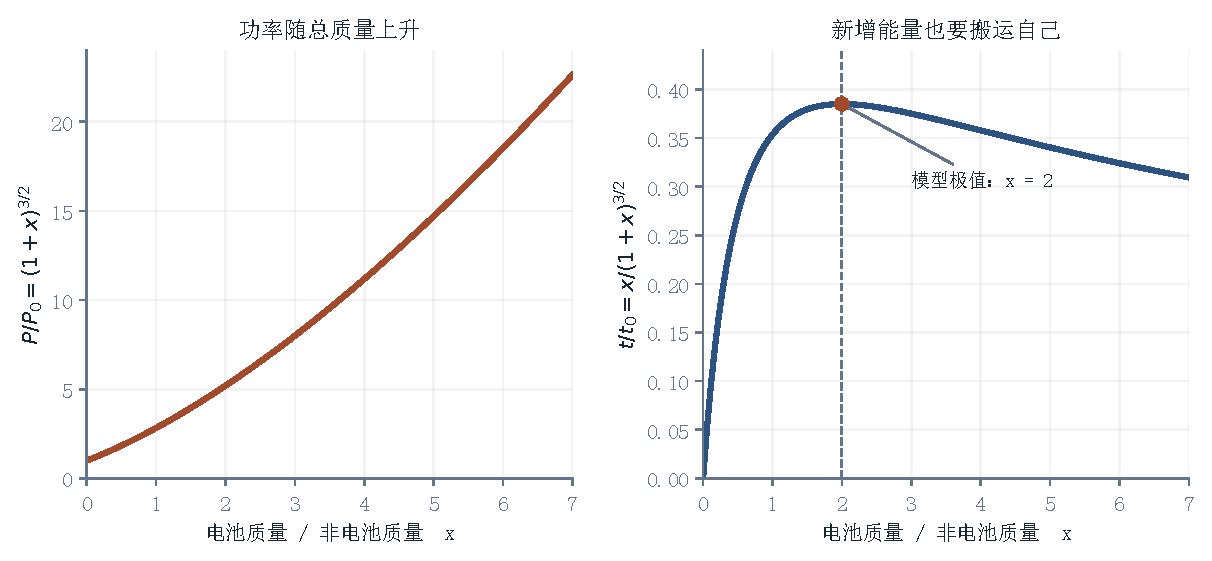
\includegraphics[width=\textwidth]{figures/hover-tradeoff.pdf}
\caption{固定桨盘面积、空气密度与效率的理想悬停模型。$x=m_b/m_0$；$P_0$为非电池质量对应的诱导功率，$t_0=\epsilon e_bm_0/P_0$。归一化续航在$x=2$达到极值。实际设计还要计入结构、功率限制与任务剖面。}
\label{fig:lift-ledger}
\end{figure}



\subsection{验证时间、场景匹配与治理层的产业价值}

\subhead{验证时间与空域耦合}

低空经济的时间刚性来自验证。它不能靠几次试飞证明成熟。飞行是高后果系统，需要飞行小时、适航认证、维护规程、事故统计、公众接受和监管信任。越接近载人、城市密集区和高频运营，验证越慢，责任越重。飞行器可以很快发布概念机，低空位移系统却不能很快获得社会信任。

飞行能力、设计符合性、单机状态和运营许可是不同层次。Joby在2026年3月宣布首架用于TIA的FAA符合性飞机开始飞行测试；9月另行公布的J208自主飞行巡展，则使用改装的Cessna Caravan与受监督运行。\cite{joby2026conforming,joby2026j208} 两项进展属于不同平台，不能合并为“自主电动空中出租车已完成全部商业准入”。FAA与EASA的框架也分别处理设计和运行要求。\cite{faa2026aam,easa2026vtol}

它的拓扑耦合来自空域。低空不是空白空间，而是城市、机场、军航、民航、公安、消防、建筑、通信、气象、隐私、噪声和公众安全共同交织的空间。飞行器越多，系统越不是“单机飞行”，而是“空域网络”。空中一旦高密度运行，风险就不再来自单个飞行器，而来自整个空域系统的协调能力。因此，低空经济不是轻资产经济，而是轻道路、重治理的位移系统。它省掉了一部分地面连续基础设施，却增加了大量空域规则、通信接口、验证体系和责任结构。它不是无摩擦未来，而是另一种黏滞分布。这也决定了它的落地顺序。

低空经济最先成熟的，不会是大众空中通勤，而是高价值、强约束、可验证的任务。电力巡检、管线巡查、农林植保、消防侦察、灾害勘察、医疗物资急送、海岛补给、山地物流、港口园区、矿区、景区、固定线路接驳，这些场景更接近低空经济的真实入口。它们运行域相对清晰，地面替代路径很重，责任边界较容易定义，运营数据可以逐步积累。反过来，大众空中通勤是最难的场景。它要求低噪声、高安全、低价格、高准点、高密度、低等待、高冗余、公众信任和监管协同同时成立。这不是造出几架 eVTOL 就能解决的问题。城市空中出租车可以出现，但它更可能先是高价、固定航线、少数场景的服务，而不是像公交、地铁、网约车那样覆盖日常生活。落地顺序由约束决定，不由愿望决定。

\subhead{场景匹配}

落地顺序确定之后，筛选标准也就清楚了。低空经济真正要避免的，不是“飞不起来”，而是场景错配。如果它用于地面拓扑过重的地方，就是有效旁路；如果用于普通地面出行，就是高成本炫技。它如果服务应急、巡检、农业、山区、海岛、消防、医疗和固定走廊，就可能降低总作用量；如果只是为了让城市中产从一个商圈飞到另一个商圈，可能只是把道路拥堵换成空域监管、噪声投诉、高保险成本和低利用率设备。因此，判断低空经济，不应先问“市场有多大”，而应先问“哪些位移值得飞”。不是所有位移都值得三维化。低空路径的价值，取决于地面路径有多重、时间价值有多高、任务风险有多大、运行域有多清晰、责任链有多完整。一个成熟产业不会把所有需求都往天上搬，而是筛选那些地面黏滞足够高、低空替代足够有优势的场景。

这也意味着，低空经济很难成为“空中私家车”。私人飞行器的利用率、安全责任、维护成本、起降接口、空域审批和事故风险，都比私家车更难社会化。真正可能成熟的形态，仍然是运营化：固定任务、固定航线、固定空域、固定维护、固定责任链。低空飞行器不是被个人占有才产生价值，而是在高频、可控、可维护的任务网络中产生价值。这一点和自动驾驶运营车相似。自动驾驶运营车的关键，不是让每个人拥有一辆无人私家车，而是用高利用率运营车辆覆盖大量日常位移；低空经济的关键，也不是让每个人拥有一架低空飞行器，而是让飞行器在高价值场景中形成稳定运营网络。

二者的差别在于：自动驾驶运营车更可能覆盖大众日常出行，低空经济更适合补足地面位移过重的特殊场景。前者重构日常交通，后者打开高黏滞场景的旁路。场景分工确定之后，产业价值沉淀的位置也就确定了。

\subhead{治理层的产业价值}

低空经济的产业价值，不会只沉淀在机体制造上。飞行器当然重要，但更重要的是空域管理系统、通信导航、起降接口、维修体系、飞行数据平台、气象服务、保险定价、适航认证、运营组织、应急处置和城市治理接口。卖飞行器只是第一层，运营低空秩序才是更深层。如果每个地方各建一套低空平台，各搞一套标准，各自招商造景，低空经济就会从第三维度的打开，变成新的碎片化工程。真正成熟的低空产业，需要统一规则、互认标准、跨区域航线、事故责任、数据接口和监管平台。否则，飞行器能飞，产业却不能规模化运行。

市场预测反映需求预期，项目收入来自实际可服务的任务。起降接口、许可、噪声约束、天气可用率与周转时间，会把总需求筛成能够经营的线路。治理层的产业价值就在这里：把一段理论可飞的路径，组织成可验证、可维护并能持续兑现的服务。

低空经济最好的状态，是成为位移系统的补充层，而不是新的万能叙事。它不应被赋予替代地面交通的使命，也不该被贬低为纯粹概念泡沫。它有真实价值，但价值来自场景匹配。它的第一原则很简单：当地面路径太重，低空路径才有意义；当飞行的治理成本低于地面绕行成本，低空经济才成立。所以，低空经济的判断标准不是飞行器能飞多远、飞多快，而是三个问题：第一，这个任务的地面位移是否足够高黏滞；第二，低空路径是否能降低单位有效位移的总代价；第三，这个低空系统是否可验证、可监管、可追责、可持续运营。答不上这三个问题，所谓低空经济就只是飞行器展示、地方口号和资本故事。答得上，它才是新的位移层。

把这条第一原则写成不等式，

\begin{equation}
A_{\text{低空}}+A_{\text{治理}}<A_{\text{地面绕行}}
\end{equation}

式中 $A_{\text{地面绕行}}$ 是完成同一次位移走地面路径所支付的总作用量；$A_{\text{低空}}$ 是低空路径自身的作用量，包含飞行器制造与折旧、能耗、维护、安全冗余和起降点；$A_{\text{治理}}$ 是第三维度的秩序成本，包含空域划分、航线审批、实时监控、通信导航、气象感知、适航验证、保险与责任结构。三项必须先折算到同一口径，并分摊到同一次有效位移上（时间、能量、风险、占地、责任），单位随口径而定，因此这是一个判定条件，而不是可以直接相加的实测量。它的含义是：低空路径的价值不由它省下了多少道路决定，而由它省下的地面代价是否大于它自己带来的总代价决定。适用边界在折算：哪些成本能进入同一个账本取决于任务本身，同一组飞行器在电力巡检或医疗急送上可能满足这个不等式，在城市商圈之间的日常通勤上可能不满足，这正是“场景匹配”的准确含义；制度合法性、公共接受与长期信任难以折算时，不等式只覆盖可折算的部分。

低空经济的本质，不是把交通搬到天上。它是在地面拓扑过重的地方打开第三维度，又在第三维度中重新支付能量、载荷、安全、监管、责任和运营代价。它的价值不在于天空看起来无限，而在于少数场景中，天空确实比地面更低黏滞。它的边界也在这里：低空不是无摩擦未来，而是一种高治理成本下的位移旁路。

\section{流态管理：让不同的时钟一起工作}

工厂、医院和交通网络都可能在局部指标改善时，让接口变得更难管理。每个环节都更快，并不保证整条链更稳。接下来的问题是：怎样让响应速度不同的过程持续协作？

\subsection{一个系统里的多只时钟}

符号可以迅速复制，变压器的交付需要更长时间，某些临床后果则要长期观察。速度差属于具体过程。神经信号很快，数字系统的训练与验证也可能很慢。比特、原子与生命各自包含快过程和慢过程。

对确定的过程$i$，可以比较它的特征弛豫时间与外部驱动周期：
\begin{equation}
De_i=\frac{\tau_i}{T_{\text{驱动}}}.
\end{equation}
$\tau_i$与$T_{\text{驱动}}$采用相同时间单位，$De_i$无量纲。这一德博拉数来自材料研究；用于组织或生物干预时，要把“弛豫”落实为可以观察的恢复过程。

接收端恢复得比驱动快，相邻变化就可能分别被吸收；驱动快于恢复，尚未完成的响应就会重叠，历史开始进入当前状态。这个比值描述时间关系，稳定性还取决于增益、延迟、反馈方向、储备和执行能力。

仓库可以每隔几秒改变路线指令，人员训练与布局调整却要更久。电网可以迅速处理电气扰动，增建容量仍需多年。药物可以很快作用于靶点，长期效果与风险还在形成。项目真正需要识别的是这些时钟及其连接方式。

\begin{table}[ht]
\centering
\caption{快过程、慢接收端与可能积累的负担}
\label{tab:ch4-three-media}
{\small
\begin{tabularx}{\textwidth}{@{}l >{\RaggedRight\arraybackslash}X >{\RaggedRight\arraybackslash}X >{\RaggedRight\arraybackslash}X@{}}
\toprule
项目层 & 相对快的动作 & 较慢的接收过程 & 可能积累的负担\\
\midrule
数字 & 生成设计、提交改动 & 集成、审查与验证 & 未验证变更、版本债务\\
工业 & 修改订单与调度 & 建造设备、形成产能 & 积压订单、长期承诺\\
生命 & 启动干预 & 适应、恢复与长期观察 & 未解决暴露、风险与随访需求\\
\bottomrule
\end{tabularx}}
\end{table}

单一时钟往往不是好设计。局部快回路处理扰动，上层慢回路调整目标，更长周期检验容量与方向。分层、缓冲与明确接口，让不同速率能够共存。

\subsection{保住可以恢复的运行区间}

长期运行的系统需要一个区间：服务能够继续，扰动能够吸收，偏离之后仍有路径回来。流态的比喻由此获得用途：观察有序通过、波动放大与关键连接失效。实际判据要落在队列长度、恢复时间、共同失效、储备与关键服务连续性上。

局部改善可能把工作点推向边界。交期缩短，留给纠错的时间减少；库存下降，缓冲变薄；政策改动太密，证据尚未形成就进入下一轮。这些措施也能改进原本低效的过程。区别在于它们改变了怎样的完整回路。

第一条路径是配速。接收端确实需要时间，就拉长对应决策周期；测量与纠偏可以加快，就提高回路响应能力。快慢的价值取决于行动能否被接住。

第二条路径是分流。库存、储备、分阶段上线、模块边界与局部自治，都能隔开一部分速率差。缓冲容量应按扰动期间“流入超过流出”的累计量估计。可以补充的储备，与只把冲击推迟一次的等待，具有不同动力学。

第三条路径是维护稳定性所依赖的功能。验证产生证据，审计暴露问题，维护保存能力，责任安排连接行动与救济。它们的价值来自实际结果。能以更少步骤完成同一功能，就是进步；留下更长流程却没有留下功能，仍然只是成本。

把可靠性、缓冲和恢复纳入目标，优化也会选择这些投入。制度问题出现在支付与收益分离的地方：维护预算记在一个部门，避免的中断却惠及整个网络；设备寿命跨过数任管理者，今天的成绩可能在别人任内结账。

\key{必须有人跨过慢周期持有这笔账。}记录、预算和责任需要足够连续，才能把当前收益与后来的支出接在一起。生态影响可能超过许可周期，技能形成可能超过产品周期，公共设施可能超过任期。系统的时间跨度，应进入决策权的安排。

本章横跨三种介质，采用的是同一套核算纪律：身体怎样吸收接触误差，机器怎样减少或转移残差，车辆怎样改变能量流，运营网络怎样使用资产，飞行怎样缩短路径又建立空域秩序。成本可以净下降。完整边界让我们看见下降发生在哪里，剩余的时间、风险和费用由谁承担。

当符号行动变便宜，这套纪律面对另一种困难。方案、凭证、图像与身份，可以生成得比核实它们更快。对象、证据与承责者一旦错开，行动就可能取得效果，却找不到与效果相称的反馈。下一章从这里开始。

\furtherreading{%
Rolf Pfeifer and Josh Bongard，\textit{How the Body Shapes the Way We Think: A New View of Intelligence}，MIT Press，2006\\
Daniela Rus and Michael T. Tolley，“Design, Fabrication and Control of Soft Robots”，\textit{Nature}，2015\\
Richard C. Lewontin，\textit{The Triple Helix: Gene, Organism, and Environment}，Harvard University Press，2000\\
Evelyn Fox Keller，\textit{The Century of the Gene}，Harvard University Press，2000\\
Herbert A. Simon，\textit{The Sciences of the Artificial}，MIT Press，1969\\
Nancy G. Leveson，\textit{Engineering a Safer World: Systems Thinking Applied to Safety}，MIT Press，2011\\
Vaclav Smil，\textit{Energy and Civilization: A History}，MIT Press，2017\\
Jarrett Walker，\textit{Human Transit: How Clearer Thinking about Public Transit Can Enrich Our Communities and Our Lives}，Island Press，2012}


% <<<<<<<<<< parts/book-ch04.tex <<<<<<<<<<


% >>>>>>>>>> parts/book-ch05.tex >>>>>>>>>>
%% ===================== 本章参考文献 =====================
\printbibliography[heading=subbibliography,title=参考文献]

\chapter{存在与坍塌：当作用量趋近于零}

位移、制造和遗传都要依赖实际条件。物理稳定、功能维持与社会责任采用不同判据：一块岩石可以被动稳定，一种服务需要持续运行，一个法律关系需要制度支持。技术改变其中一段的成本，会重新安排关联结构，也让“它以什么方式存在、凭什么被依赖”成为具体问题。

生命之所以会对干预作出反应，是因为它必须持续维持自身。这种反应不是被动受力，而是把外部作用转成自身维持过程的一部分。把这一点放到更长的时间尺度上，它并不只是生物学事实。任何能够持续存在的东西，都在以某种方式对抗溃散，而维持自身的代价由什么承付，决定了它在现实中占有多重的分量。

\section{存在的判据：什么算存在，什么可以被依赖}

存在、知识与责任分别要求不同的判据。一个对象可以真实存在，却不构成可靠证据；一个判断可以成立，却没有获得执行授权；一个系统可以造成后果，却没有相应的承受边界。机器生成把这几种关系推到前台。区分它们，才能说明轻载体如何抵达重后果，以及哪一步缺少了必要的凭据或责任。

\subsection{存在的重量：从物理稳定到智能生成}

\subhead{稳定与切分}

世界最初没有图像，也没有名字，甚至没有我们今天意义上的“物”。在极早的宇宙中，结构尚未稳定，能量、场、粒子和涨落交织在一起，存在还不是对象，而是连续的相互作用和不稳定的差异。后来，宇宙膨胀，温度下降，原子形成，恒星点燃，元素合成，行星冷却，世界才逐渐从混沌的能量状态中沉淀出稳定结构。存在的第一步，不是被命名，而是稳定下来；没有稳定结构，就没有可以被反复指认的东西，也没有“这个东西”与“那个东西”的区别。

稳定有不同的维持条件。岩石的结构取决于化学键、晶格和环境，行星轨道取决于运动状态与引力关系；这些稳定未必要求持续的外部做功。生命则通过代谢、修复和调节维持远离平衡的状态，组织依靠人员、记录与制度持续运行。存在的物理条件、功能的维持成本和社会责任由此分开，后面要分别追问它们如何被支持。

生命出现以后，世界不再只是外部环境。最早的生命并不拥有世界模型，它只是在化学梯度中维持边界，摄入能量，排出废物，修复损伤，趋近有利条件，远离破坏条件。对生命来说，感知不是为了描绘世界，而是为了继续存在。同一片水域，对岩石只是环境；对生命体，却可能是资源、威胁、温度、压力和通道。世界没有改变，但某些差异开始被生命内部的维持过程选出来。不是所有存在都同样重要，只有那些影响代谢、修复、移动和生存的差异，才进入生命的世界。

智能的本体论根源就在这里。智能不是凭空面对一个已经切分好的对象世界；现实本身是连续的过程、流动、扰动、能量差和物质分布。智能首先要做的，不是求解，而是在连续现实中切出可行动的差异：什么可以接近，什么必须避开；什么可以摄入，什么会伤害；什么是路径，什么是障碍；什么是自身，什么是外部。所谓“对象”，不是世界天然贴好的标签，而是稳定结构与行动需求相遇后形成的切分。生命按代谢和危险切分，动物按路径、猎物和威胁切分，人类按名称、工具、制度和责任切分。智能的差异，首先不是答案不同，而是把什么东西当成“一个东西”的方式不同。

表示由此萌芽。足迹、气味、巢穴、叫声、姿态和迁徙路线，不是图像，也不是文字，却已经让不在场的东西继续发生作用。一个气味标记让离开的身体仍然影响后来者，一条路径让过去的移动影响下一次移动，一种叫声让危险在危险到来之前被传递。任何能让不在场之物继续影响行动的结构，都已经具有表示的影子。存在不再只在现场发生，它开始留下可被其他生命读取的痕迹。

人类把这种替代能力推进到新的层级。声音、手势、图案、刻痕、壁画，让事物第一次以可保存、可传播、可重排的形式出现。一头野牛不只在草原上存在，也开始在洞穴墙壁上存在；一次狩猎不只发生在现场，也开始在讲述中延续；一条河流不只流经土地，也开始进入方向、记忆和传说。神话、文字、账本、地图、法律和数字进一步扩大了这种能力：债务、土地、税赋、边界、王权和法律都可以离开现场，进入符号、记录和制度。一个命令可以跨越距离，一个账目可以跨越时间，一个法律可以在制定者死后继续约束行动。

\subhead{两种重量}

这时，世界中出现了一类新的存在。债务不是石头，法律不是身体，货币不是粮食，国家不是山川，但它们并不因此虚无。它们存在于记录、承认、执行、预期和责任之中\cite{searle1995construction}。它们没有自然物的直接质量，却能组织岩石、粮食、道路、矿山、军队和人的一生。这里必须区分两种重量：一种是物理重量，来自质量、体积、材料和能量；另一种是\term{本体论重量}，来自确立、维持、执行、回滚、外溢和承责的代价。社会性存在物理上可以极轻，却可能在现实中极重；它们轻于质量，却重于结算。

更准确地说，存在的重量不是一个单一刻度，而是由几种承付关系构成：确立、维持、回滚、外溢和承责。物质结构重在材料与能量，生命过程重在代谢、复制和不可逆扩散，社会结构重在承认、执行和信任，主体结构重在后果能否回流到一个持续边界中。所谓轻与重，不是价值高低，而是结算条件不同。把这几项支出加总，
\begin{equation}
W=w_{1}+w_{2}+w_{3}+w_{4}+w_{5},
\qquad
\frac{\partial W}{\partial w_{3}}>0,\quad
\frac{\partial W}{\partial w_{2}}>0
\label{eq:ontic-weight}
\end{equation}
式中 $W$ 是存在物的重量，不作绝对测量，只用来在同一套口径下比较大小，因此无量纲或随所选口径带量纲；$w_{1}$ 到 $w_{5}$ 依次是确立、维持、回滚、外溢、承责五项承付关系各自结算出的代价，五项必须折到同一口径（工时、能量、货币或注意力，任选其一）才能相加；$w_{3}$ 对应回滚，$w_{2}$ 对应维持。两个偏导说的是只增不减的两条方向：一个东西越难撤回、越难清除后果，$w_{3}$ 越大，$W$ 也就越大；一个东西越需要持续投入才能不退回噪声，$w_{2}$ 越大，$W$ 同样越大。五项在不同层次上的权重并不相同，这才是轻重的真正来源：同样一笔结算，落在物质结构上主要由 $w_{1}$ 与 $w_{2}$ 承担，落在主体结构上则主要由 $w_{3}$ 与 $w_{5}$ 承担。

科学、工程和计算把这种分层推到新的深度。一座桥可以先存在于图纸中，一座城可以先存在于规划中，一个分子可以先存在于模型中，一个气候系统可以先存在于仿真中。图纸不是桥，公式不是机器，模型不是现实，但它们让人类能够在物质动工之前排列可能性。计算机的特殊性在于，它不只保存表示，还能运算表示：文字、图像、声音、地图、账本、公式和图纸，都可以转化为比特；模型可以被修改，参数可以被调整，未来可以被推演，现实可以在行动之前被转化为候选空间。这类存在既不属于材料，也不属于纯粹虚构，它们的重量要按另一套条件结算；机器智能把这类存在的数量推向新的量级。

\subhead{生成物的层级}

层级说明的是不同存在的重量，机器智能改变的则是生成。它把这条道路推到了新的强度。过去，生成一个世界需要神话，生成一座城市需要图纸，生成一个人物需要小说，生成一个分子需要实验室，生成一个制度需要漫长的政治想象。现在，文字、图像、声音、代码、角色、方案、药物候选、城市规划和未来情景，都可以在模型中快速出现。表示不再只是保存现实，也不只是预演现实，而开始大规模生成可能的现实。但这并不是一个全新的本体论问题。人类很早就知道，图纸不是桥，地图不是土地，法律文本不是社会秩序，货币符号不是粮食本身，小说人物不是现实人物。机器智能的特殊性，不在于第一次提出“生成物是否存在”，而在于它让表示性存在以远高于以往的规模和逼真度膨胀，把一个古老问题推到日常生活和技术系统的前台。

把生成物按层级摊开之后，追问的方向就变了。真正的问题不是：被生成的东西算不算存在。这个问题太粗。答案也太简单：它们存在，但以某种方式存在。

一个被生成的城市，作为图像和方案存在；它还没有土地、建筑、道路、居民、产权、维护和财政。一个被设计的分子，作为候选结构存在；它还没有合成、纯化、代谢、安全性、剂量和临床后果。一个仿真中成功的机器人动作，作为模型状态存在；它还没有摩擦、碰撞、磨损、误差和责任边界。一个语言中完整的人格，作为叙事对象存在；它还没有身体、时间连续性、后果回流和责任承担。它们不是不存在，而是存在于较轻的层级。

智能时代真正尖锐的问题，不是虚拟物是否存在，而是它存在于哪一层、经由哪条边进入现实、由谁承付后果。一个东西可以作为文本存在，作为图像存在，作为代码存在，作为仿真存在，作为候选存在，作为物理结构存在，作为生命过程存在，作为社会制度存在，作为责任对象存在。不同层级的存在，承受不同约束，要求不同维持条件，具有不同回滚难度。表示性存在能被说出、画出、生成、复制和修改；物质性存在要占据空间、承受负荷、消耗能量、维护结构；生命性存在要代谢、修复、适应、复制并反馈；社会性存在要被承认、执行、信任和追责；主体性存在则必须在时间中维持边界，并把行动后果重新带回自身。层级之间如何通行，由此成为比层级本身更紧的问题。

\subhead{重量与可达性的解耦}

技术黏滞与本体论在这里相接。技术黏滞不只是技术执行慢，不只是组织保守，也不只是资源不足。它更深的含义是：轻存在向重存在转换时，必须穿过材料、自由能、时间、结构、验证和责任。表示空间中的城市、分子、动作、制度和人格，可以快速生成；现实空间中的城市、药物、能力、制度和主体，必须承受世界的结算。机器智能降低的是候选出现的成本，不是目标层级的存在重量。

因此，存在结构不只是一座阶梯。阶梯说明了不同层级的重量：表示较轻，物质更重，生命更重，社会与主体承担更多结算条件。但智能暴露出另一个更重要的事实：层级之间不是只能逐级通过，它们之间还有\term{转换边}。有些边很重，有些边很轻；有些边过去几乎不存在，现在被技术打开；有些边看似低阻，实际把代价转移到别处。一条转换边之所以显得低阻，往往不是因为代价消失了，而是因为代价被延迟、外包，或转移到当下尚未显明的承受结构中。

层级与边分开之后，一个系统的位置就可以被确定。一个智能系统的本体论身份，不由它的技术架构决定，而由它的转换签名决定：它从哪一层生成，向哪一层结算，经过哪条边，谁承付维持代价、回滚代价和责任后果。生成式智能主要打开表示到社会的低阻边，文本、图像、角色和模型输出可以直接进入注意力、信任、舆论、组织流程和群体判断。具身智能打开表示到物质行动的执行边，模型策略一旦接入传感器、控制器和执行器，就必须面对摩擦、惯性、碰撞、能耗、误差和安全边界。还有一条更重的边，是表示进入生命过程：序列、结构和调控方案一旦被生命系统稳定读取、表达、复制，并进入遗传或生态传播，就不再只是候选，而进入代谢、发育、繁殖、演化和生态后果。

机器智能的本体论新意，不是制造了新楼层，而是改变了存在转换图的连边结构。更准确地说，\key{它让重量和可达性解耦。}旧世界里，重存在通常难以抵达：桥梁、城市、药物、制度、身份、责任，都需要材料、时间、组织、执行和承认，越重越慢，越重越难到达。机器智能打开的新通道，使某些轻载体能够低成本抵达高后果层。一个生成物自身可以很轻，但一旦改变人的选择、关系、预期和责任分布，它就在社会层变重；一个策略本身可以很轻，但一旦驱动车辆、机械臂或无人机，它就进入物质结算；一个序列本身可以很轻，但一旦被生命过程读取并复制，它就进入更深的不可逆性。

\subhead{重量的归属}

这不是轻存在逃过了结算。结算只是发生在别处：发生在人的注意力中，发生在平台规则中，发生在组织决策中，发生在信任结构中，发生在物体受力中，发生在生命过程里，发生在后来很难撤回的行为路径中。一个生成物自身可以很轻，但它调动的反应可以很重；它的载体可以被删除，但它造成的后果未必能回滚。因此，存在重量不能只看创建代价，也不能只看载体能否删除。更重要的是维持代价、后果回滚代价，以及这些代价最终归属于何种承受结构。最危险的存在形态，恰恰可能是载体极轻、后果极重。

更进一步，重量不是无主属性。物理重量的承受者是物理本身，岩石的质量不依赖人的承认，桥梁的承重和疲劳也不会因为无人相信而消失。但社会重量不同。债务重，是因为有人承认它、追索它、执行它；身份重，是因为制度和他人承认它；货币重，是因为交换网络承认它；机器角色重，是因为用户投入注意力、情绪、信任和时间。越往社会层和主体层走，重量越不是内在属性，而是关系量。同一个机器角色，对深度依赖它的人极重；对不识别它的系统几乎为零。同一个模型输出，对把它写进决策流程的组织极重；对外部旁观者只是文本。判断一个生成物是否变重，不能只看它的创建代价，也不能只看平台运行代价，还要看它的维持代价由谁承付。

智能还带来了另一种变化：表示开始形成自循环。过去，表示大多来自现实。地图来自土地，图纸指向工程，账本对应交易，照片来自现场，模型需要经验校准。今天，生成内容进入数据，数据训练模型\cite{shumailov2024ai}，模型继续生成内容，生成内容再进入人的注意力、平台分发和下一轮信息环境。表示不再只是现实的影子，而可能形成自我复制的回路。这不是虚拟替代现实，而是分叉：表示层可以在现实校准不足的情况下自我繁殖，同时又借助平台、关系和信任进入社会层，产生真实后果。最危险的形态，不是一个虚拟世界完全取代现实，而是一个没有充分现实校准的表示环境，持续影响人的判断、关系和行动。

在生命过程里，类似逻辑更重。一个进入生命过程的候选结构，如果被稳定读取、复制、遗传、扩散和选择，就可能不再依赖原始设计者持续维持。它开始沿着生命自己的机制传播。此时，智能生成的不是普通表示，而是进入自我复制过程的入口。这不是说智能可以任意创造生命。生命空间受到代谢、发育、稳定性、繁殖、生态和演化的强约束，可组合不等于可存活，可设计不等于可延续。真正的重量，不在序列被写出，而在它是否能被生命过程读取、维持、复制，并产生难以回滚的后果。

\subhead{本体论作为操作}

从这个角度看，本体论不是智能之外的抽象哲学，而是智能本身的底层操作。智能并不是在一个已经切分完成的世界里活动。它首先要把连续现实分解成可识别、可记忆、可预测、可操作的单位。生命把世界切分为有利与有害，动物把世界切分为猎物、威胁、路径和同伴，人类把世界切分为名称、工具、制度和责任，科学把世界切分为变量、模型、尺度和系统，计算机把世界切分为数据结构、状态空间和算法对象。机器智能则把这种切分推进到大规模生成、快速转换和跨层结算。

但这里隐藏着更深的裂缝。人类的本体论习惯于对象、边界、身份和责任。我们用“一个人”“一件物”“一个组织”“一个行为”“一个后果”来切分世界。可是机器智能的内部表示不完全以人类熟悉的离散对象为单位，它在很大程度上更接近连续空间中的方向、相似性、分布和可插值区域。它生成的对象，是人类界面上的对象；它内部处理的，未必是人类意义上的对象。人类需要对象，因为行动、责任、法律和记忆都依赖边界；机器智能可以在连续表示空间中处理相似性，却把结果输出成我们能理解的对象。这个差异暂时被界面掩盖了：我们看到的是图像、文本、角色、方案和回答，以为它在使用同样的本体论。但它内部执行的切分，未必与人类用来承担责任的切分一致。

因此，机器智能真正打开的问题，不是它生成了什么，而是它把多少轻载体送入了高后果层级，却没有同时生成相应的承受边界。一个模型可以影响公共判断，一个算法可以改变价格、排序、流量和机会，一个自动代理可以下单、筛选、推荐、拒绝、调度和执行，一个机器角色可以成为人的情感对象和决策参照。它们在社会层产生后果，却未必在主体层承受后果；它们可以参与行动，却没有身体，可以产生后果，却没有生命史，可以影响他人，却没有内在承受，可以被依赖，却没有稳定责任边界。

这些既产生后果又不受后果约束的存在物，撞上了社会的一条旧规则。传统社会默认一个基本等式：行动者应当也是承责者。自然人如此；公司、组织和国家虽然不是自然身体，但也通过法律、制度、财产、代表和责任链建立了责任结构，能够被起诉、惩罚、约束、解散、赔偿和追责\cite{dewey1926historic}。机器智能让这个等式松动了。开发者、部署者、平台、用户、组织、模型本身都可能参与后果链条，但责任在它们之间分散、转移、稀释，最后变成无人完整承受的残差。更深地说，机器智能的可回滚性，是它能力的一部分，也是它无法自然承责的原因。它可以快速生成、复制、替换和重置，因此能以极低成本参与判断和执行；但承责需要相反的东西：一个会被后果改变、不能随意逃逸、能够在时间中持续的边界。

这就是本体论通向主体论的地方。机器智能制造的不是一个简单的“像不像人”的问题，而是一类有社会后果、物质后果甚至生命后果，却未必有主体边界的存在物。它们不是虚无，也不是完整主体；不是普通工具，也不是传统制度法人；不是生命，却能进入关系；不是承责者，却能改变后果。智能时代最危险的本体论错误，不是相信虚拟物“存在”，而是忘记它落在哪一个存在层级上、靠哪一条边维持、又由谁承担它维持不住时的代价。

从宇宙太初到机器智能，存在的历史可以被看成一条漫长的分层之路，也是一条不断开辟新通道的路径。这条道路没有错。没有表示，现实只能被动发生；有了表示，现实可以被预演、计划和改造。智能之所以强大，正是因为它能让世界在行动之前先变成可处理的对象。

但这条道路也有边界。表示越轻，越容易忘记现实的重量；生成越快，越容易低估转换的代价；智能越能制造可能性，越需要区分可能性所在的层级，识别通向现实的路径，并追问后果由谁承受。世界可以被表示得越来越快，但现实仍然要求存在被材料承载，被时间展开，被生命反馈，被社会承认，被责任接住。生成不是终点。存在要被维持，后果要被回滚，责任要有承受者。

到这里，问题不再只是“什么存在”，而是：代价归属于何处，谁在维持，谁在行动，谁来承受。而在追问代价归属之前，还有一个更早的问题需要回答。被切分、保存、传播和生成的这些表示，究竟凭什么能够被依赖。

\subsection{知识的凭据：候选之后，什么能够被依赖}

表示被说出、保存和依赖的规模越大，它凭什么可以被依赖，问题就越硬。存在可以按层级摊开，一种东西可以很轻，却仍然抵达很重的后果层；在这一步之前，还有一件更早的事需要交代：在后果真正发生之前，行动所依据的判断凭什么站得住。

\subhead{校准先于命题}

知识不是世界本身，也不是表示本身\cite{ogden1923meaning}。世界并不因为被理解才运行，表示也不因为被说出就成为知识。对生命来说，最早的“知道”不是命题，而是校准：什么能接近，什么会破坏；什么能维持边界，什么会带来损伤。错误不是逻辑问题，而是生存问题。把毒物当成营养，代价不是观点被反驳，而是结构被破坏。由此看，知识从一开始就不是纯粹观看，而是在世界约束下形成可依赖差异的过程。

这里讨论的\term{凭据}，首先指向那些会被依赖、会指导行动、会进入现实后果链的知识。纯数学和形式逻辑是一个极限情形：它们的凭据主要来自证明、结构一致性和公理边界\cite{godel1931}，而不是经验接触；但只要它们被用于工程、计算、金融、治理或科学建模，就会重新进入现实后果链。换言之，凭据的形式可以不同，但任何被依赖的判断，都必须说明自己在何种结构内成立、何时可以迁移、何处必须停止。人类让校准离开身体，进入语言、文字、图像、数字和制度记录。经验因此可以传播、积累和复用，也可以伪造、漂移和固化偏见。真正重要的不是人类会说，而是人类逐渐发明了让说法接受约束的方式。测量让感觉进入尺度，实验让判断暴露在结果面前，复现让一个说法不能只依赖某个权威，数学和仪器把直觉无法稳定分辨的差异压入可比较、可推演、可检验的结构。科学的特殊之处，不在于它让人类说出了更多东西，而在于它发明了一套让世界有机会拒绝人类说法的机制\cite{popper1934logik}。

\subhead{凭据的两层结构}

从这个意义上说，知识不是一种更漂亮的表示，而是一种获得凭据的表示\cite{gettier1963justified}。凭据不是由流畅性、完整性、自洽叙述或权威语气授予的，而来自两层结构：第一层是形成层，即接触、校准、复核；第二层是兑现层，即边界和后果。接触让候选暴露于约束，校准让误差返回判断结构，复核让判断离开单点输出；边界说明它在哪里成立、在哪里失效，后果说明它被依赖之后会改变什么、由谁承受什么代价。两层缺一不可：只有形成过程而没有边界与后果声明的候选，无法说明自己何时失效；只有后果要求而没有接触与复核的判断，只能靠权威维持。

凭据如何形成？不同介质会改变凭据形式，但不改变基本结构。接触让候选暴露于对象、材料、身体、环境、行为或结构约束；校准让误差返回判断尺度，使下一次判断因此改变；复核让判断离开单点输出，进入不同主体、工具和场景的公共检验。成熟知识不是无边界的自信，而是知道自己在哪里成立、在哪里失效；一个判断一旦被依赖，就会进入行动，改变路径、资源、身体、组织和未来。没有后果要求的候选可以作为想象、草案、启发或游戏；一旦进入身体、工程、交通、金融、治理或生命过程，就不能只凭形式完整获得通行。

凭据的形成与兑现不排斥机器，它们只是规定了机器能做什么。机器当然可以参与验证。它可以运行测试，比较数据，发现异常，辅助复核，搜索反例，执行仿真，检查一致性，甚至在某些封闭环境中完成高度自动化的确证流程。问题不在于机器能不能参与验证，而在于验证的最后代价由现实接触设定，验证的充分性标准则由后果结构决定。合成要接触材料，治疗要接触身体，交通要接触道路，工程要接触负荷，生命干预要接触代谢与生态，制度设计要接触人群行为。机器可以加速某些环节，却不能自动决定“多少凭据才算足够”，因为这个问题最终要回到边界、后果、风险和承受者。

因此，智能时代的知识问题，不是机器是否“真的理解”。这个问题仍然绕在人类心智的旧词汇里。更稳的问题是：一个输出是否被置于足够的接触、校准、复核、边界和后果约束之中；它是否知道自己的适用范围，是否能够暴露来源，是否能够标明条件，是否能够在失败时被追踪，是否能够被现实修正。知识不是一个孤立答案，而是一条可追溯的形成路径。这条路径的起点不在表示内部，而在表示之外的接触、工具、场景和制度。

\subhead{候选扩张与凭据带宽}

机器智能改变了这条历史的压力分布。从认识论结构看，它是文字发明以来规模最大的一次表示技术扩张。文字让记忆离开身体，人的认识位置从背诵转向理解、辨析和解释；印刷让复制脱离手抄，人的认识位置从占有文本转向筛选、校验和诠释；计算让形式推演和搜索脱离心算，人的认识位置转向模型边界、数据来源和结果验证。机器智能延续并放大了这条线：它降低的不是知识成立的成本，而是候选出现的成本。正因为候选可以被大规模、低成本地提出，人类在认识论中的位置并没有消失，而是从答案的生产者转向凭据结构的设计者、边界的判断者，以及可依赖性本身的形成者。

更具体地说，机器智能没有首先取消无知，而是极大扩张了候选空间。这里的候选不只是文本回答或屏幕图像，也可以是解释、代码、控制策略、实验方案、分子结构、蛋白构象、交通路径、诊断判断、金融操作、制度草案，乃至进入生命过程的序列和调控方案。智能制造的不是已经成立的知识，而是有待检验的可能路径。介质不同，约束不同，验证方式不同，但认识论问题是同一个：这些候选凭什么被依赖？

\key{智能扩张候选，验证形成凭据。}

这句判断的两侧，现在可以分别结算了。这是智能时代认识论的核心，也是上一节“重量与可达性解耦”在认识论上的对应面。前面说的是轻载体如何低成本抵达高后果层；这里讨论的是候选如何低成本出现，却未必携带相应凭据。存在论上，问题是轻东西如何产生重后果；认识论上，问题是快候选如何获得慢凭据。机器智能真正改变的，不是让生成自动等于存在，也不是让生成自动等于知识，而是把可能性出现的速度同现实承付的速度分离开来。过去，稀缺常常在信息获得；现在，许多领域的表述能力、组合能力和搜索能力被急剧放大，稀缺开始转移：不再是有没有说法，而是哪一个说法经过了足够约束；不再是有没有路径，而是哪一条路径可以被依赖。更准确地说，机器智能使\term{候选通量}与\term{凭据带宽}发生解耦：候选出现的速度被大幅提高，而接触、校准、复核、边界和后果仍然受材料、身体、时间、制度和责任限制。由此产生两类相反的失败：在存在层面，轻载体可能已经抵达高后果层，却没有明确承受者；在认识层面，候选尚未穿过现实，却已经冒领了知识外形。

把这两个速率写进同一个流量关系，

\begin{equation}
\frac{dQ}{dt}=\lambda_{\text{候选}}-\lambda_{\text{凭据}}
\end{equation}

式中，$Q$ 是尚未穿过接触、校准、复核、边界声明和后果检验的候选存量，单位为个；$t$ 是时间，单位为年；$\lambda_{\text{候选}}$ 是候选出现的速率，$\lambda_{\text{凭据}}$ 是凭据形成的速率，二者单位均为个每年，故右侧量纲回到个每年。这个式子的含义是：解耦不需要额外的机制，它只是两个速率不再相等。当候选出现的速率高于凭据形成的速率时，存量按两者之差单调增长，而增长的存量不会自己生成凭据；这就是“不缺说法、缺的是可以被依赖的说法”的结构形式。适用条件是两侧必须折算到同一粒度，候选与凭据只有在能按同一种单位计数时，差值才有意义；而且它只给出趋势方向，不给出长期预测，因为存量增长会反过来改变筛选标准、注意力分配和制度安排，$\lambda_{\text{凭据}}$ 本身随存量变化。它刻画的是结构，不提供任何实测数值。

\subhead{形式外壳与认识论黏滞}

可依赖性因此成为新的核心稀缺。一个回答可以很快，一个判断不能因此可靠；一个解释可以圆满，一个机制不能因此成立；一个动作可以在仿真中成功，一个真实系统不能因此安全；一个序列可以被写出，一个生命过程不能因此可控。机器智能让候选获得了知识的外形，却没有自动给予它被依赖的凭据。危险也正在这里：错误不再必然粗糙，无知不再必然沉默，虚假不再必然破绽明显。它可以流畅、礼貌、系统、专业，并且在表面上完成所有表达动作。因此，这不是简单的“幻觉”问题；更深的变化是候选的生产机制与确证机制发生了分离，形式的完成速度超过现实的校准速度，可能性的展开速度超过凭据的形成速度。

这种变化会改变人类对知识的直觉。人类长期把流畅表达、概念组织、语气稳定、格式规范和逻辑连贯当作可信信号，因为在过去，这些信号通常需要训练、经验和制度背景才能产生。机器智能打破了这种关联：它保留了可信信号的外壳，却降低了外壳的生成门槛。于是，认识论的任务不再只是区分有无信息，而是区分候选是否获得凭据。在这个意义上，技术黏滞也可以被理解为认识论黏滞。不是世界拒绝智能，而是世界要求判断付出接触成本；不是现实落后于生成，而是现实要求任何候选在被依赖之前先承受约束。生成可以在表示空间中快速展开，验证必须接触世界；生成可以并行制造大量候选，验证必须面对材料、时间、实验、身体、场景、制度和责任。生成常常是轻的，验证却会变重，因为验证要让候选穿过现实的阻力。

表示自循环的本体论后果已经讨论过：表示可以在现实校准不足的情况下自我繁殖，并通过平台、关系和信任进入社会层，形成一种轻载体、重后果的存在分叉。这里要看的是它的认识论后果。一个认识系统如果主要从自身的回声中获得材料，就会逐渐削弱接触比例；它可能越来越擅长内部一致，越来越不擅长承受外部反驳。仿真、指标、模型、平台反馈和组织报告，都可能形成类似的自我喂养回路\cite{cinelli2021echo}。系统越是用内部生成物替代外部接触，就越可能形成高度一致的候选世界，却不再知道现实从哪里打断它。知识不是被现实支持的漂亮表示，而是保留了反驳接口、并能把反驳转化为校准的候选。

\subhead{验证的分配}

候选爆炸之后，真正困难的还不只是验证，而是验证如何被分配。接触世界需要材料、实验、时间、场景、组织、注意力和责任，不可能平均分配给所有候选。因此，人类的新认识角色不是逐一验证所有输出，而是在候选洪流前设计验证路径：哪些候选因为后果不可逆而必须优先检验，哪些候选因为越出边界太远而必须暂缓依赖，哪些错误因为暴露延迟而需要更高等级的复核，哪些判断只能停留在启发层，哪些可以进入行动准入。验证不是单纯的技术动作，而是一种稀缺接触预算的分配。这也是人类知识制度的价值所在。图书馆、实验室、大学、标准体系、期刊、审计、临床试验、工程认证、事故调查、法院证据、同行批评，并不是知识之外的附属物，而是凭据形成和验证分配的结构\cite{merton1942normative}。它们缓慢、昂贵、烦琐，有时保守，有时僵化，但它们承担一个基本功能：防止任何流畅的表示、漂亮的模型或成功的仿真绕过接触，直接冒充可依赖的判断。

机器智能不会让这些结构消失，相反会使它们更重要。当候选说法稀少时，人类可以把大量注意力放在生成上；当候选空间膨胀时，人类必须把更多注意力转向筛选、验证、追溯、边界判断和验证优先级。未来真正稀缺的能力，不只是提出答案，而是为答案建立凭据；不只是生成方案，而是知道方案需要通过哪些现实约束；不只是给出结论，而是判断哪些结论值得消耗昂贵的现实接触。验证预算有限，这决定了认识论的主要工作从生产转向排序。

所以，智能时代的认识论不能只问真假。真假当然重要，但更第一性的问题是：这个候选经过了什么约束？它的凭据从哪里来？它能被谁复核？它的失败如何暴露？它的边界如何声明？它一旦被使用，会进入什么后果链？

如果这些问题没有答案，那么它最多是候选，而不是知识。候选并不低贱，人类所有知识都从候选开始；但候选不是终点。认识论的核心任务，就是不要让候选未经凭据化就伪装成知识，不要让形式的完整性冒充现实的通过。

这也意味着，人类在智能时代的认识角色不会消失，而会改变。人不再只是答案的生产者，而越来越成为验证路径的设计者、边界的判断者、接触预算的分配者和可依赖性本身的形成者。机器可以扩大候选，也可以执行大量验证环节；但哪些候选值得接触现实、哪些判断可以被依赖、多少凭据足以行动、哪些后果必须被优先看见，这些问题最终会回到主体、价值和承受者。只有把机器智能放在正确位置上，它才真正强大：把候选当成知识，会制造虚假的确定性；把候选放回候选，则能极大扩展探索空间。

这就是问题核心：候选之后，什么能够被依赖？答案不在于它是否最流畅、最像专家、最符合期待、最能安慰人，也不在于它是否最快给出结果。这些只是表达层面的外观，不能构成知识的凭据。真正能够被依赖的，是那些经过接触、校准、复核、边界声明和后果检验的判断、结构与路径。知识不是语言的胜利，而是候选在现实约束中存活下来的形式。机器智能之后，人类面对的不是知识自动丰收，而是候选空前丰盛。真正稀缺的，是让候选穿过现实、形成凭据、成为可依赖判断的能力。从这里开始，问题不再只是“什么被生成”，而是：什么能够被验证，什么可以被依赖，什么可以获得进入行动的准入。

\subsection{行动的准入：表示何时可以跨过转换边}

候选之后，需要凭据；凭据之后，仍然不能直接行动。知识与行动之间不是一条连续斜坡，而是一条转换边。知识使一个判断获得可依赖性，行动则使这个判断进入现实过程。前者仍然处在表示关系之中，后者已经开始改变世界状态。一个模型可以有统计优势，一个方案可以通过局部测试，一个控制策略可以在仿真中稳定，一个制度设计可以在理论上自洽，但这些都还没有回答更重的问题：它是否可以消耗资源、占用时间、触碰身体、调动组织、改变制度，并使残余后果落到具体承付结构上。

\subhead{转换边}

前面两节分别讨论了存在的重量和知识的凭据：轻载体可以抵达高后果层，重量与可达性被机器智能重新拉开；候选可以高速生成，但凭据不能同速形成，候选通量与凭据带宽发生脱钩。到这里要处理的是第三个断裂：表示可以获得现实触发力，却不自动携带后果承付结构。核心问题不是“能不能输出”，也不只是“能不能被相信”，而是一个表示在什么条件下可以触发现实状态转移。

\key{触发力与承付结构的解耦，是行动论在机器智能时代遇到的新问题。}

承付结构在传统世界里由行动者本人提供。行动通常与一个有限主体捆在一起。一个人做出行动，不只是发出一个指令或表达一个愿望，而是把身体、身份、声誉、责任、时间和未来押入某条路径。行动者不是纯粹的触发点，也是后果回流的边界。失败会改变他，损失会落到他身上，责任会追溯到他，未来义务会继续缠住他。正因为行动者自身被押入后果，行动才不是轻飘的表示，而是有重量的选路\cite{arendt1958human}。

机器智能改变的不是这个结构的意义，而是它的耦合方式。模型可以生成指令、调用工具、修改文件、发送信息、执行代码、访问数据库、触发审批、改变排序、调度设备。它可以通过权限、接口和工作流触发现实变化，但这些变化未必回流到模型本身。模型可以拥有触发力，却没有身体损伤；可以参与路径选择，却没有生活世界；可以放大后果，却没有资产边界、声誉连续性和惩罚敏感性。触发发生了，承付却不在同一边界内完成。

\subhead{行动论的边界}

这就是为什么传统行动论既重要，又不能主导本章。传统行动论长期追问：什么使一个事件成为行动？行动是否由意图、理由、欲望、信念或计划组织\cite{davidson1963actions}？一个行为为什么可以归属于某个行动者？这些问题背后真正处理的，是行动归属与后果回流的耦合。意图、理由和计划并不只是内心事实，它们把“为什么选这条路”“谁在选路”“谁延续这个选择”连接起来。一个有计划的行动，是主体用未来约束现在，也是把后果提前纳入自身连续性\cite{anscombe1957intention}。

AI agent 使这个框架遇到边界。问题不必首先落在“AI 是否拥有真正意图”上。即使没有传统意义上的完整意图，系统仍然能够触发现实状态转移。它可以移动资金、驱动设备、触发流程、传播信息、改变排序、重排机会。于是行动论的问题发生偏移：不再只是“这个行为是否属于某个主体”，而是“某个表示通过什么接口进入现实，获得了多大作用半径，并由什么结构承付它的残余后果”。

这也是近年 AI agent 使风险形态发生变化的原因。普通生成模型首先带来内容风险：错误、幻觉、偏见、误导、伪造。agent 则把问题推进到行动边界：权限、身份、日志、回滚、停机、监控、持续运行和责任范围\cite{openai2025chatgptagentsystemcard}。过去，模型输出离行动很远，中间隔着阅读、理解、转写、审批、执行、复核等多重摩擦；现在，读、写、查、调、改、发起、调用和执行可以被连成同一条工作流。模型不只是说出可能性，而是在某些接口中获得触发力。

这说明，agent 的实质不只是模型更聪明，而是表示跨过转换边的摩擦被降低了。过去，组织摩擦在无形中延缓了错误进入现实；今天，自动化把这种摩擦压缩为权限调用。过去，一个建议要经过人类转译才可能行动；今天，建议、调用和执行可以在同一系统中连续发生。风险焦点因此从“表示是否正确”转向“表示如何获得触发力”。行动准入也因此不再是伦理附录，而是机器智能进入现实系统的第一边界。

\subhead{知识与行动的分界}

要把这一点说清楚，必须区分知识与行动。知识降低不确定性，行动花费不可逆性。验证消耗的是接触预算，行动消耗的是不可逆预算。一个判断越可靠，越有资格被依赖；但被依赖仍不等于可以执行。因为判断仍然属于表示空间，行动则进入现实历程。表示空间允许多个候选并存，现实系统只能沿具体路径演化。一个方案进入执行，其他方案就被延迟、排除或失去条件；一个政策进入实施，社会激励就开始重排；一个医疗方案进入身体，代谢和免疫过程就已经启动。知识管的是“能否信”，行动管的是“是否花掉一段不可逆”。

行动不是知识的应用，而是不完备知识对现实的暴露。任何行动都不可能等到未来完全展开之后才发生。再充分的凭据也只能降低不确定性，不能把未来全部提前完成。行动发生时，总有一部分残余不确定性从模型、文本、计划或仿真内部转移到现实系统之中。这个转移不是修辞意义上的风险，而是结构意义上的状态改变：未知后果开始由身体、设备、市场、组织、制度或生态过程承载。

因此，行动的重量不来自动作本身，而来自它对可达空间的处分。表示空间可以容纳很多尚未实现的可能；行动则把其中一条路径实际化，同时消耗资源、占用时间、改变结构，并关闭一部分未来可能性。一个医疗建议变成用药，身体就进入特定代谢路径；一个交易策略变成自动执行，风险就进入市场结构；一个招聘模型变成筛选规则，某些人的机会空间就被提前收缩；一个调度策略进入电网、交通或工厂，物理系统就必须沿它给出的节奏响应。即使局部后果可以回滚，时间、机会、信任、损伤和路径依赖也不能完全恢复为行动之前的状态。

\subhead{行动与可达空间}

这使讨论重新回到结构与可达空间。第二章讨论的结构记忆已经说明撤回不等于恢复；同一章的可达空间分析已经说明系统并非在无限可能中自由移动，而是在历史路径、鲁棒性和结构约束中保留有限可塑性。行动正是可达空间被花掉的动作。每一次不可逆行动，都在某种程度上改变未来可达域。机器智能让选路、触发和执行变得更轻，因此也让“花掉不可逆性”变得更容易。如果没有准入，系统会以很高速度消耗自己的可塑性。

这也把行动准入接回 RTG 模型。行动一旦发生，R 不再只是资源估算，而是资源被实际占用、锁定或消耗；T 不再只是等待或验证周期，而是不可逆历程；G 不再只是结构关系图，而是被实际牵动的反馈、耦合和责任链。行动是 RTG 从分析坐标变成现实结算的时刻。它把可能路径转换为现实路径，也把模型残差转换为系统残差。

把行动放回 RTG 之后，还要区分它穿过的是哪一种边，因为不同转换边具有不同重量。表示进入社会判断，首先改变注意力、信任和预期。错误图像、伪造引用、看似专业的解释、被自动分发的结论，可以进入人的信念结构，继而改变组织和公共讨论。这里的后果不一定表现为直接物理伤害，而是判断环境被污染。

表示进入物理执行，后果更直接。控制策略一旦接入车辆、机械臂、电网、无人机、工厂或医疗设备，就不再只是概率分布，而是力、热、速度、位移、碰撞、磨损和故障。表示进入生命过程，转换边更重。生命不是被动载体，而是会读取、代谢、放大、修复、抵抗、代偿和演化的过程。表示进入制度决策，后果最容易被低估。一个评分模型进入招聘，一个风险模型进入信贷，一个预测系统进入警务，一个分配算法进入教育或医疗，都不是单纯提供建议，而是在重排人的可达空间\cite{oneil2016weapons}。

\subhead{承付的重建与持续准入}

因此，行动准入不能被理解为“多加一层安全要求”。它的功能，是在触发力与承付结构被切开的地方，人工重新缝合它们。旧世界里，主体常常免费提供这道闸门：行动者把自己押入后果，行动因此天然带有重量。机器智能使触发可以脱离这种押入，准入就必须把承付结构重新挂回行动点。没有这个重建，行动就会成为无承付的触发。

把承付挂回行动点有几种做法。可验证、可停止、可回滚、可追溯、可承责，不是平铺的治理清单，而是重建承付结构的不同方式。没有验证，残差不可识别；没有停止，残差不可中断；没有回滚，残差不可收束；没有追溯，残差不可定位；没有承责，残差没有回流边界。它们共同回答的不是“系统是否合规”，而是“未消除的不确定性进入现实后，是否有承载、收束和回流结构”。

准入不是给知识盖章，而是在触发之前重建承付。

据此可以说，“人在回路中”本身不够。关键不在于人是否形式上出现，而在于人是否拥有真实的承付位置。一个只能点击确认的人，不是准入者，只是自动化流程中的责任垫片。一个看不见模型边界、看不见后果链、无法改变执行路径、又必须在极短时间内确认的人，不是在监督系统，而是在替系统承担名义责任。有效监督要求人能够看见边界、理解残差、改变路径、中止过程，并实际处在后果回流链条中\cite{santoni2018meaningful}。

更困难的是，转换边常常不是一次性跨过的。很多系统开始只是辅助，后来成为推荐；开始只是推荐，后来成为默认；开始只是默认，后来成为自动；开始只是自动，后来变成无人真正理解和质疑的基础设施。表示不是突然变成行动，而是被界面、流程、绩效压力和组织惯性逐步推近现实。最后出现的不是一次越界，而是一条已经固化的路径。

对于持续运行的 agent，行动准入也不能只发生在部署之前。能够调用工具、读取反馈并调整策略的系统，不是在执行一次动作，而是在形成一条持续作用的因果管道。准入必须规定作用半径、权限边界、更新频率、监测方式、停机条件和责任回路。一次测试通过，只能说明系统在某些条件下可以开始，不能说明它在所有未来反馈中都拥有不受限制的行动权。持续行动需要持续准入。在这个意义上，准入评价的不是一个表示是否精彩、连贯或有启发性，而是它获得触发力之后，是否具备相应的承付结构。若剩余不确定性找不到明确的承担者，表示仍可作为候选、解释、模拟或辅助存在，但不应获得现实执行权。行动的门槛，不是知识的完成，而是残差的可承付化。

到这里，前面的线索合在一处：轻载体如何抵达重后果，快候选如何获得慢凭据，表示获得现实触发力时又如何必须重建承付结构。否则，机器智能会生成更多候选，也会更快花掉不可逆性，更快压缩系统可达空间，并把残差外部化给那些没有准备承受它的身体、组织和制度。行动把残余不确定性推入现实，并使其落在某些位置上；但后果落在哪里，并不等于谁在承受。身体、市场、组织、平台、部署者、用户和受影响者都可能被迫承载后果，却未必形成清晰的回流边界。于是，行动准入之后，问题必然推进到下一层：什么样的边界，才有资格被称为后果的承受者？

\section{承受的边界：后果回到哪里}

行动一旦发生，后果就要落到具体的人、组织和环境中。产生后果的位置与承受后果的位置可能分离，控制权与责任也可能被分散。本节所讨论的责任主体，需要有稳定身份、可追索资源、记录和后果回流机制。人的人格地位与基本权利另有伦理和制度依据，责任结构则回答一次行动由谁解释、纠正和赔偿。

\subsection{主体的边界：后果回流与责任显现}

行动把残余不确定性推入现实之后，承付必须落在一个边界上，而“边界”本身在思想史上有很长的来路。在人类很长一段思想史里，最先被追问的不是主体，而是世界本身。什么存在，什么是真实，变化背后有没有稳定结构，万物如何成为万物，这是本体论的问题。那时，人当然也在世界之中，但人还不是问题的中心；人首先面对的是一个比自己更大的秩序：自然、神、实体、形式、规律、宇宙结构。问题的重心在“世界如何成立”。

\subhead{从本体论到主体论}

后来，问题开始转向人自身。世界不只是存在在那里，还要被经验、被认识、被判断、被表达。于是，主体被推到前台。不是因为世界消失了，而是因为世界进入人的经验和判断以后，必须追问：谁在认识？认识凭什么可靠？判断从哪里获得确定性？这个转向把人从世界中的一个位置，变成了世界显现和意义生成的中心之一。主体不再只是存在者之一，而是世界如何被把握的条件\cite{kant1781kritik}。

再往后，问题又从认识推进到行动。人不只是看世界、解释世界，也在改变世界。技术、工业、科学实验、组织、工程和制度，把人的判断变成了现实中的力量。于是，仅仅问“谁在认识”已经不够，还要问“谁在行动”。行动不同于认识，因为行动会改变状态，会制造不可逆后果，会让世界不再只是对象，而成为被干预、被重构、被损伤或被修复的过程。现代智能把这个问题继续往前推了一步。智能系统不只生成表述，不只辅助认识，也开始参与行动：它可以生成判断，触发流程，操控机器，参与实验，影响交通、医疗、金融、教育和生命过程。问题因此不再只是“谁在认识世界”，也不只是“谁在改变世界”，而是：改变发生以后，后果回到哪里？

这就是从本体论到主体论，再到行动论和承受论的真正来路。本体论问世界如何存在，认识论问世界如何被把握，行动论问世界如何被改变，而主体论在智能时代必须追问：改变之后，反作用由谁承受。过去，意图、身体、行动和后果大多绑定在同一个生命或制度边界里；现在，生成、执行、收益和损害可以分散到不同位置。行动发生了，世界被改写了，反作用却未必回到制造差异的地方。所以，主体问题不是因为机器开始像人说话才重新尖锐，而是因为智能进入现实以后，作用与反作用开始脱钩。一个边界如果只向世界施加差异，却不被差异的后果反过来改写，它就还不是完整主体，而只是无主行动中的一个发生点。\key{主体不是意识叙事的中心，而是后果回流的边界。}

上一节讨论的是行动准入：一个候选、判断、方案或指令，什么时候可以跨过表示层，进入现实系统。这里追问的是下一步：一旦行动进入现实，反作用回到哪里？没有准入，行动会过早发生；没有主体边界，行动会无人承受。智能时代的问题不是行动太少，而是行动越来越容易被生成、触发和放大。真正稀缺的，是让行动重新接回承受边界的能力。

\subhead{后果回流的边界}

主体不是会说“我”的东西。会自称，会解释，会表达偏好，会生成计划，会承认错误，都只能制造主体的外形。主体也不是单纯能行动的东西。能行动只说明它能向世界施加差异，不能说明差异造成的反作用会回到它自身。

主体首先是作用与反作用闭合的地方：行动从这里发出，后果回到这里，代价在这里沉积，未来行动因此被约束。所以，主体不是行动的起点，而是后果的归宿。一个大模型可以输出判断，一个具身系统可以执行动作，一个生命智能可以提出干预方案；这些都还不够。关键在于，错误、损伤、失败、羞耻、信任破裂、声誉变化、身体代价、时间损失和未来限制，是否会回到同一个持续边界中。没有后果回流，就只有输出；没有代价沉积，就没有主体。

这里必须区分反馈和承受。反馈可以很轻。温控器有反馈，控制系统有反馈，模型可以根据错误更新参数，机器人可以根据碰撞调整路径\cite{wiener1948}。反馈回答的是系统如何修正，如何提高效果。承受不同。承受意味着代价回到行动者身上，留下不可随意擦除的痕迹，并改变它未来能够如何行动。参数更新不是悔恨，路径重规划不是负责，损失函数下降不是付出代价。反馈是信息回流，承受是代价回流。主体从承受开始，而不是从反馈开始。

承受从哪里开始，人的身体给出了最直接的例子。人的身体之所以天然形成主体边界，不是因为人有某种神秘特权，而是因为人的生命过程足够难以逃离\cite{merleauponty1945}。一个人犯错，会痛，会羞耻，会失去时间，会破坏关系，会改变声誉，会在记忆中反复返回那个后果。人不能像模型一样轻易重置版本，不能像零件一样无痛替换，不能把衰老、伤害和死亡外包给另一个实例。人之所以天然接近主体，不是因为人更高贵，而是因为人不能无成本逃离自己。

\subhead{两种承受封装}

所谓\term{承受封装}，就是后果不能随意散开。身体记得伤口，神经记得恐惧，习惯记得重复，关系记得背叛，声誉记得选择，时间记得不可逆。一个“我”不是一句自我叙述，而是后果在身体、记忆、关系和时间中不断回流、折叠、压实之后形成的持续边界。主体不是静止内核，而是被过去行动不断改写的连续性。生命主体不能每次行动后彻底清零，只能带着沉积过的后果继续行动。

具身智能容易制造一个误解：机器有身体、能感知、能行动，所以就获得了主体性。这不成立。机器人的外壳、关节、传感器和执行器构成物理边界，但物理边界不自动等于主体边界。机器可以损坏，零件可以更换，模型可以替换，机体可以报废，数据可以回收，成本可以转移。许多后果并不回到机器自身，而是散落到制造者、使用者、部署者、环境和被影响的人身上。身体如果只是执行器，就不是主体边界；身体只有成为后果沉积的地方，才具有主体意义\cite{dreyfus1972what}。

生命体不同。生命体的身体不是临时接口，而是长期演化形成的承受结构。许多复杂性被封装在形态、反射、疼痛、恢复、习惯和有限寿命中。机器没有自然继承这笔演化摊销。它可以拥有行动能力，却不必然拥有承受能力；它可以进入空间，却未必把空间中的反作用带回自身；它可以改变身体，却未必承受身体被改变后的余波。这就是具身性和主体性之间必须划开的边界。

反过来，没有自然身体，也不意味着完全不能形成主体。一个组织没有疼痛，没有肉身，没有生命意义上的死亡，但它可以通过资产、账目、历史记录、声誉、身份和长期约束形成某种制度边界\cite{dewey1926historic}。它过去的行动会改变它未来能做什么，能获得什么信任，能承担什么限制。后果可以在制度中沉积，制度也可以因此被过去改写。这说明主体不是生物身体的专利。主体可以由生命封装，也可以由制度封装。关键不在材料，而在后果能否在一个边界内持续闭合。

\subhead{无主行动与责任显现}

闭合成立与否，在多数智能系统上一眼可见。当前多数智能系统的问题，不是它们“不像人”，而是它们的闭合边界尚未成立。大模型能生成判断，但判断造成的后果不自然回到模型；具身系统能执行动作，但动作的反作用不一定沉积在机器自身；生命智能能提出干预方案，但被分类、筛选、治疗和优化的人，才真正承受长期结果。智能越能生成、行动和干预生命，越会放大这个缺口：差异由系统制造，反作用却由别处承受。这不是简单的“谁负责”问题，而是更底层的“行动是否有主”问题。没有主体边界，行动会退化为输出；没有承受闭合，现实会退化为反馈数据；没有代价回流，错误会被分摊到看不见的地方。一个系统可以越来越有效，却越来越不承受；可以越来越会行动，却越来越像没有主人。要防止的，正是这种世界被纯输出化的趋势。

责任显现也不应被理解成外部条款。它的深层意义，是让被系统吞掉的后果重新可见。当行动只影响行动者自身，反作用常常自然显现：摔倒会疼，失败会记住，关系会破裂，时间无法倒流。但当行动通过模型、机器、组织和生命技术放大到更大范围，后果就可能被延迟、遮蔽、统计化、转嫁，变成没有一处真正疼痛的损失\cite{matthias2004responsibility}。责任不是事后装上的道德标签，而是主体边界在社会中的显现。它让行动不能只留下效果，也必须留下归处。

主体性因此不是非有即无的标签，而是后果回流的闭合强度。工具几乎没有闭合，锤子伤人，后果回到使用者。普通代理体有目标和反馈，却未必有承受。制度主体没有自然身体，却可以让后果在组织记忆和长期限制中沉积。生命主体拥有最强的承受封装，身体、记忆、关系、衰老和死亡把后果锁在同一个生命过程中。未来也可能出现工程化主体，但那不取决于它会不会说“我”，而取决于它是否拥有持续身份、不可任意重置的记忆、真实代价沉积、外部可追问边界和长期未来约束\cite{parfit1984reasons}。主体论不是为了捍卫人的神秘性，也不是为了预先否定机器可能获得某种主体地位。它要提出的是判准：谁被行动的反作用持续改写，谁才开始接近主体；谁只负责施加差异，却总能把代价转走，谁就仍然只是通道。智能时代真正危险的不是机器像不像人，而是行动越来越多，后果越来越散，世界开始出现大量无主行动。

主体不是会说“我”的东西。主体是后果不能再继续转嫁的地方。它把行动、反作用、记忆、代价和未来约束重新扣在一起。没有这个边界，智能系统会越来越能改变世界，却越来越难被世界反过来改变；行动会越来越多，主人却越来越少。但还有一个入口没有被检验。机器可以拥有身体，能感知、能执行、会磨损、会自我维护，这些能力常被读作主体性的证据；如果主体性只取决于后果能否在一个边界内闭合，那么材料边界与承受边界就必须分开来看，而工程上完全可以把身体做强的那些条件，恰恰未必等于承受闭合形成的条件。

\subsection{承受闭合：从机器身体到工程化主体}

而工程上出现了一个更容易误判的问题：机器有了身体，能感知、能行动、会磨损、会自我修复，是不是就更接近主体。这个问题之所以重要，是因为智能进入现实有几种不同入口。大模型让输出进入社会判断，具身智能让身体进入材料世界，生命智能让方案进入代谢、发育、免疫、遗传和生态过程。它们都比单纯的屏幕文字更重，也都更容易让人误以为：智能越接近现实，就越接近主体。

\subhead{现实入口不是主体边界}

但现实入口不是主体边界。一个系统可以输出判断，却不承受判断造成的后果；可以拥有身体，却不承受身体行动造成的代价；可以提出生命干预方案，却不承受代谢、发育和代际后果。进入现实只说明作用发生了，不说明反作用已经回到同一个持续边界。主体性不从输出中自然长出，不从身体中自然长出，也不从生命干预能力中自然长出。主体性只在一个地方显现：后果是否回流、沉积，并约束同一边界的未来。

因此，首先要把身体、具身性和主体性拆开。身体是材料边界，回答系统以什么物理结构进入世界。具身性是材料边界与环境形成行动耦合，回答系统如何感知、耗能、受扰、修正和继续行动。主体性是后果回流和承受闭合，回答行动之后，代价是否回到一个不能随意逃离的连续边界。三者相连，但不能互相替代。

身体可以被工程化。传感器可以增加，执行器可以升级，关节可以维护，材料可以柔顺化，能量可以调度，局部控制可以低延迟，自诊断可以常态运行。未来机器身体甚至可能具备更强的自维护和自修复能力：检测磨损，修补表面裂纹，重新分配能量，在局部损伤后降级运行\cite{terryn2017self}。但这些首先仍然是身体工程，不是主体生成。

上述区分可以写成一个只刻画回流覆盖面的比率。设 $B$ 是一个持续边界，$a$ 是它发起的行动，$C(a)$ 是该行动的全部后果，$\rho_a$ 把每一项后果映射到最终承载它的边界。定义 $B$ 在行动 $a$ 上的后果回流比例

\begin{equation}
\kappa(B,a)=\frac{\bigl|\{\,c\in C(a):\ \rho_a(c)=B\,\}\bigr|}{\lvert C(a)\rvert},
\qquad \kappa\in[0,1].
\label{eq:ch33-closure}
\end{equation}

这里假定$C(a)$是有限、非空且分项一致的集合，$\rho_a$把每项归于一个边界。$\kappa$只记录这份清单上的回流覆盖。实际后果可以共同承担，也可能无法计数；分项方式和权重都会改变结果。这个比率帮助追问归属，不测量意识、道德地位或完整主体性。保险和公共救济还可能正当地分担后果，不能把全部回流当成普遍目标。

\subhead{残差吸收与后果承受}

这里必须区分残差吸收和后果承受。具身系统进入物理世界以后，滑移、摩擦、惯性、接触误差、传感漂移和任务链偏差都必须被处理。它们可以被身体吸收，被控制器修正，被环境约束，被外部支撑结构分担。残差吸收解决的是行动能否继续。后果承受追问的是行动归属于谁。具身性容易被误读，正因为它把这两个问题压得很近：机器真的在处理现实残差，于是看起来也像在承受现实后果。

但一个东西被现实改变，不等于它在主体意义上承受现实。石头会风化，桥梁会疲劳，轮胎会磨损，电池会衰减，数据库会被写入，模型会被微调，机器会留下日志。它们都在时间中留下痕迹，但这些痕迹未必构成一个行动者的历史。被改变只是物理事实，承受则意味着后果被纳入一个可追问的连续性。这里的关键差异，是承载和承受。轮胎承载摩擦，机械臂承载反力，电池承载放电循环，外壳承载碰撞和磨损。只要机器进入物理世界，后果就会落到某些部件上。但承载只是后果落在\term{承载面}上；承受要求这些后果进入同一持续边界，改变它的未来可达空间，并使它不能无成本逃离过去。

一个服务机器人撞坏墙角，外壳可能划伤，轮组可能偏移，日志可能记录异常，控制策略可能更新。物理后果落在了机器上，信息反馈也回到了系统里。但真正的反作用可能落在用户、制造者、部署者、空间环境和被影响的人身上。机器身体只是后果链中的承载面，不必然是后果链的归宿。它受到了影响，却未必成为承受者。所以，承受至少包含几项条件：后果回到同一边界，而不是只落到可替换部件；后果改变这个边界的未来可达空间，而不是只触发维修或参数调整；行动带来的增益、限制和反作用约束同一连续体，而不是向不同位置散开；这个边界能够被外部持续追问，而不是在版本、实例、供应链和维护链条之间消失。少了这些条件，机器身体即使有磨损，也只是后果经过的材料界面，不是后果归属的主体边界。

\subhead{自我保护与生命封装}

很多讨论把“会保护自己”看成主体性的证据，这同样需要拆开。机器人会避障，不等于它害怕受伤；会低电量返航，不等于它关心未来；会检测故障，不等于它理解自己的脆弱；会自我修复，不等于它承受了创伤。避障可以是控制目标，返航可以是能量策略，自修复可以是材料机制。它们可以很复杂，也可以很有效，但它们首先是在维持功能，不是在形成一个不能逃离自身的“我”\cite{metzinger2003being}。生命体为什么不同？不是因为生命体内部藏着一团神秘主体，而是因为生命把承受封装得更深。

身体、代谢、疼痛、恢复、发育、记忆、关系和死亡，把后果压进同一个不可随意替换的过程。身体受伤不是单个部件异常，而会改变行动能力和未来时间；疼痛不是报警灯，而是把损伤带入同一个生命边界；死亡不是报废外壳，而是连续性的终止。生命不是更高贵，而是更难把代价转走。生命体不能随意更换完整身体，不能把记忆无痛迁移到另一个实例，不能在失败后从干净版本重新启动，不能让一个等价副本替自己承受衰老和死亡。主体性不是从会动的肉体里长出来，而是从不能无成本逃离自身的连续性中长出来。

机器身体没有自然继承这条连续性。它可以有编号、位置、外壳、传感器和维护记录，却仍然可能只是一个可替换实例。关节磨损了，可以换；模型出错了，可以回滚；机体报废了，可以用同款机器接替；策略失败了，可以在新版本中擦除。机器当然可以有历史，问题在于，这些历史常常属于平台、车队、制造商、外部运行结构或数据库，而不属于执行个体自身。历史被记录，不等于历史被承受。

\subhead{承受闭合的条件}

这不是说机器永远不可能形成主体性，而是说主体性不能由身体自动推出。未来若出现某种工程化主体，它需要的不是更像人的外形，也不只是更精密的触觉皮肤，而是承受闭合的工程：持续身份，不可任意重置的历史，真实代价沉积，未来行动受过去后果约束，外部能够追问的边界，以及不能把所有代价转嫁给用户、部署者、环境和受影响者的结构。这样的结构可以不是生物性的。组织没有自然身体，却可以通过资产、声誉、法律身份、历史记录和长期约束形成制度边界。它没有疼痛，却有后果沉积；没有肉身，却有身份终止。主体性不是肉体专利，但它要求后果不能随意散掉。

这也解释了智能进入现实的三种错位。大模型的错位，是表示能够影响现实判断，却不承受判断后果；具身智能的错位，是身体能够承接现实残差，却不必然归属行动代价；生命智能的错位，是方案能够进入生命过程，却未必承受代谢、发育、遗传和生态的长后果\cite{floridi2013distributed}\cite{nissenbaum1996accountability}。越往后，承受面越重，系统自身却未必更像主体。风险不在于智能越来越像人，而在于智能越来越能进入高后果层，却仍然可以把代价留在别处。

因此，判断一个智能系统是否接近主体，不应看它像不像人，也不应只看它有没有身体，而要看它是否形成了承受闭合。一个系统可以高输出而低主体，可以高度具身而低主体，也可以深入生命过程而仍然没有承受闭合；反过来，一个组织没有自然身体，却可以通过制度形成主体边界。表示是现实影响的入口，身体是材料耦合的入口，生命技术是生命过程的入口，主体性则是后果回流和承受连续的闭合强度。

\subhead{耦合、自我修正与可替换性}

更底层地看，智能系统进入现实有几种不同耦合。表示耦合回答系统能生成什么候选、影响哪些判断。材料耦合回答系统能否在物理世界中稳定行动。生命耦合回答一个方案进入生命过程以后，会被什么生命结构读取、放大、抵抗、沉积或传播。承受耦合则回答后果是否回到一个持续边界。前三种耦合说明智能如何进入现实，最后一种耦合才触及主体性。

这也解释了为什么“自我修正”仍然不是主体性。大模型可以反思输出，具身系统可以监测磨损并主动安排维修，生命智能系统可以根据实验结果更新候选、优化剂量、调整干预路径。它们看起来都在改正自己，但改正不等于承受。只有当错误不能只是变成新版本、新策略、新疗程或新候选，而会以不可转嫁的方式改变同一持续边界的未来，修正才开始接近承受。

更深的分界在于可替换性。身体作为工程对象，天然倾向于模块化、可维护、可替换、可复制。工程追求降低单点不可替代性：坏了能换，错了能回滚，实例能迁移，能力能复用，影响能隔离。这对可靠性是好事，却恰恰削弱了主体性的自然生成。主体需要某种不可完全替换的连续性，而工程常常通过可替换性提高系统韧性。机器越是良好的工程对象，越未必是主体。

这不是矛盾，而是两种目标的分叉。工程身体追求可维护，主体边界要求可追问；工程系统追求故障隔离，主体性要求代价沉积；工程结构追求实例迁移，主体性要求身份连续；工程优化追求外部影响最小化，主体判准追问反作用最终回到哪里。身体可以被设计得越来越强、越来越灵活、越来越自洽，但只要后果仍然由别处承受，它就还是进入现实的通道，而不是后果的归宿。

\subhead{不可逃离的边界}

这正是“身体可以工程化，主体不能自然继承”的精确含义。工程化身体的目标，是把现实扰动处理掉，让系统少停机、少损坏、少失控；主体边界的目标，不是把后果处理掉，而是让后果不能失踪。一个方向追求残差被吸收，另一个方向追问代价由谁保留。工程越成熟，越可能把故障消隐在维护、替换、冗余和外部支持结构中；主体性越清晰，越要求这些被消隐的后果重新回到可追问边界。两者可以相互支持，但绝不能互相推出。

最硬的判准在这里：\key{主体性不看系统能否保护自己的部件，而看它能否逃离自己的后果。}一个系统如果能把伤害分散给用户，把风险交给外部结构，把错误归入版本，把损坏交给维护，把身份迁移到新实例，而自己继续作为干净能力出现，它就还没有成为主体。相反，如果某个边界不能这样逃离，过去行动会持续限制它、定义它、追问它，并改变它未来能够进入的路径，那么即使它不是生物，也已经开始接近主体。

主体不是身体的自然升级版。身体让机器进入世界，具身性让机器在世界中形成行动闭环，生命技术让智能进入更重的生命过程；但主体性要求世界把行动的后果带回同一个持续边界。它不从传感器里长出，不从执行器里长出，不从生命干预能力里长出，也不从自我描述里长出，而从代价无法继续转嫁的地方显现。因此，主体性不能从任何一种现实入口中自然推出。输出、身体、反馈、自维护和生命干预，都只能说明系统已经以某种方式接入现实；它们还没有说明后果会回到哪里。只有当反作用持续回到同一个边界，并改变它未来能够如何存在、如何行动、如何被追问时，这个边界才开始具有主体意义。具身性让机器进入现实，承受性才让一个边界成为主体。

不过，单个边界的闭合只是判准的一半。一次行动很少只穿过一个边界：平台、开发者、部署者、组织、用户和受影响者各自承担了一部分后果，回流路径不止一条，收束点也不止一个。当后果分散在多条回流路径上时，闭合究竟在何处成立，谁来决定哪个边界承担哪一部分，代价又如何在多个承受者之间分配，这些还没有答案。

\subsection{分布式承受：为什么公司能负责而模型不能}

上一节停在了一个没有答案的问题上：当后果分散在多条回流路径上时，闭合在何处成立，谁来决定哪个边界承担哪一部分。要回答它，可以先看一个已经把这件事做完的例子。有一种主体，不吃饭，不呼吸，没有神经系统，没有经历，也没有痛苦。它可以拥有财产，签订合同，被起诉，被罚款，被强制解散。它要为自己的行为负责。这种主体叫公司。

\subhead{一个已经解决的难题}

公司承担责任这件事，今天已经不再让人惊讶，以至于它的构造性被忽略了。公司不是自然物。它是一组法律装置人为组装出来的承受边界。人们花了几个世纪才把这组装置拼齐，其中最关键的一步是有限责任：投资人以其出资额为限承担责任，公司以其全部资产承担责任，两者分开。有限责任常被当成一种鼓励投资的经济政策。它在结构上的作用更基础：它把一条本来会无限延伸的后果链，截断在一个可以清点的边界上。在这条边界内，有资产可以扣，有账户可以查，有代表可以传唤，有主体可以解散。因为边界存在，追责才成为一个可以操作的动作，而不是一场无限追溯。

这提供了一把尺子。用它可以量出，一个系统要成为后果的承受者，需要什么条件。用这把尺子去量机器智能系统，缺什么就很清楚了，但在那之前，先要把这把尺子本身说清楚。

\subhead{承受边界的四个条件}

把公司的结构拆开，可以看到四件事同时在起作用。第一是\term{可清点的资源边界}。公司有自己的资产和负债。赔偿不是象征性表态，而是从资产负债表上真实划走一笔。资源边界让惩罚具有量纲。第二是\term{稳定的同一性}。公司持续存在，跨年度、跨管理层、跨员工流动。今天的公司要为十年前的公司行为负责，因为它们被认定为同一个法律人格。同一性是追责的时间通道。

第三是\term{受罚后的内部状态改变}。罚款会减少可投资金，影响信用评级，抬高融资成本，压缩薪酬空间，甚至触发破产。也就是说，惩罚会真正改变这个边界未来能够做什么。这是承受的实质：不是被指向，而是被改变。第四是\term{可追索的责任链}。公司有董事、高管、法人代表、雇员和股东，各自有明确的职权范围和责任分配。

一次行为可以被拆解到具体的决策位置，而不是消失在集体里。这四条加在一起，构成了一个完整的承受结构。\key{公司能负责，不是因为它有意识，而是因为制度把后果固定到了一个可追索边界上。}这四条不是同等重要的四条，而是缺一不可的四条：任何一条空着，承受结构就不成立。

\subhead{模型缺什么}

用同一把尺子量机器智能系统，缺什么就很清楚了。第一，缺资源边界。一个模型没有资产。它可以被罚款吗，罚款由谁支付？如果由部署它的公司支付，那承受者就是公司，模型本身没有承受任何东西。这一点看似只是会计问题，实际上是结构问题：没有可清点的资源，惩罚就无法落到系统身上，只能落到系统之外的人身上。

第二，要查明同一性由谁保存。模型版本变化不必然切断责任：部署者可以保留版本、配置、记录与持续义务。真正的问题是改版以后，既有行动能否仍被定位，承担义务的边界是否继续存在。

第三，要查明制裁实际改变谁。罚款减少机构资源，服务限制改变运营能力，模型更新则改变行为。几种反应可以相互连接，但承担费用和义务的通常是人或机构。把它们统称为“模型受罚”，会遮住实际落点。

第四，缺可追索的责任链。这不完全是技术问题。模型的生成、微调、部署、集成、调用和使用，常常分布在不同的主体之间。一个输出进入现实，中间可能经过模型提供方、应用开发者、平台运营方、终端使用者和受影响的第三方。每一段都有责任缺口，而责任在传输中会衰减。

把这种衰减写成逐层传递的形式，

\begin{equation}
R_n=R_0\prod_{i=1}^{n}\alpha_i,\qquad 0\le \alpha_i\le 1
\end{equation}

其中 $n$ 是行动经过的层数，无量纲，正文给出的典型情形是六到七层；$R_0$ 是行动刚发生时可归属到行动位置的责任，为便于比较可归一化为一；$\alpha_i$ 是第 $i$ 层向下一层传递之后、仍然能够归属到具体决策位置的责任份额，无量纲，取值在 0 与 1 之间；$R_n$ 是经过全部层之后仍然落在某个可追索边界上的责任份额。这个式子的含义是：只要每一层都截留一部分，剩余份额就随层数按乘积下降，层数越多下降越快，这正是“责任在它们之间分散、转移、稀释，最后变成无人完整承受的残差”的写法。它也解释了集中归属与举证责任倒置为什么有效：这两种制度处理并不减少层数，而是从外部把某些 $\alpha_i$ 抬回到接近 1。适用条件是各层贡献可分离，且不在多层之间重复归责；当同一主体同时提供模型、应用与平台时，乘积链条合并，$n$ 减小，衰减随之减弱。它标出的是结构位置，不是实测比例，$\alpha_i$ 本身无法直接测量。

通常部署的模型是责任安排中的一个组件，而非独立的法律承受者。持续身份、资源与权限可以由外部架构配置，义务和救济则需由制度确定。问题应逐项落到具体系统：谁控制、谁记录、谁获益、谁补偿。不能从当前模型缺少某种安排，推出任何工程化边界原则上都无法具备它。

\subhead{分布式承受}

真正的问题因此不是“模型能不能负责”，而是当行动分散到多个位置之后，后果应该被固定到哪里。这个问题在几个领域已经出现过。自动驾驶的碰撞责任要在整车制造商、软件提供方、传感器供应商、高精地图服务商、车主和驾驶员之间分配。同一场事故，不同的技术架构会导出不同的责任划分。

内容平台的责任要在发布者、平台、推荐算法和用户之间分配。平台以中立通道自居时，推荐算法的编排作用如何计入，长期没有一致答案。算法决策造成的差别对待，受害者要证明什么才能立案，被告要证明什么才能免责，举证责任的分配直接决定了这类案件是否可诉。这些案例的共同结构是：行动被拆散了，承受边界却没有同步拆散，也没有重新组装。发起、执行、获益和受损分处不同位置，而后果需要一个落点。

在传统结构里，这个落点由行动者本人担任。一个人做出行动，身体、身份、声誉、时间和未来都押在这条路径上，失败会改变他自己。机器智能接入之后，路径照样可以被启动、被执行、被放大，但这些动作不落在任何一个会因此改变的边界上：模型这一侧没有与行动者本人相当的位置，也没有哪个部分会随失败而改变。缺失的部分不会自动长出来。它只能由制度装置地从外部装上。

而一旦装上，人的位置就跟着变了。分布式承受被解决的过程，同时是责任从个体身上被移走的过程。当系统能够承接后果，个体与后果之间的直接联系就松了一环。松掉的那一环，原本是许多人的价值来源。如果价值曾经附着在“后果落在自己身上”这个位置上，那么松掉的一环就需要新的解释：当制度能够承接后果时，还有哪些判断必须由人来作出。价值不会消失，但它需要一个新的源点。

不过，制度接住后果的过程，最先改变的不是价值的论证，而是每个人对自己位置的判断。在价值需要一个新源点之前，先要发生的是一件更直接的事：许多人发现，自己原来用来证明价值的方式失效了。

\section{第一层塌陷：功能性危机}

存在、凭据、准入、承受，前面两节讨论的都是结构；结构的变化要落到人身上，才会显示出它真正的代价。这一步的落点不在收入，也不在岗位，而在一个更早的位置：一个人原来用什么证明自己在这个系统中占有一个位置。这一层的变化发生得最快，也最容易被误读成个人问题。
\begin{figure}[ht]
\centering
% >>>>>>>>>> figs/fig-collapse-spiral.tex >>>>>>>>>>
% 图 5-1  三层塌陷：变化速度依次放慢，察觉难度依次上升
% 三层不是三个并列的问题，而是一条因果链：功能层的真空把人推向别处，
% 别处提供的是一组保留刺激、取消做功的系统，在这种环境里边界不再被使用。
% 左侧色块给出每层的变化速度与察觉难度，右侧盒子给出机制与落点。
% 三层的颜色由 terra 经 rust 到 forest，只表示深度递增，不表示价值高低。
\begin{tikzpicture}[x=1cm, y=1cm, font=\small,
  bx/.style={rounded corners=2pt, line width=0.7pt},
  st/.style={rounded corners=1.5pt, line width=0.5pt},
  tt/.style={font=\small\heiti, anchor=west},
  tx/.style={font=\scriptsize, text=ink, anchor=north west, align=left},
  sl/.style={font=\scriptsize, text=slate, anchor=center, align=center},
  cy/.style={font=\scriptsize, text=ink, anchor=west}
]
\useasboundingbox (-0.20,0.40) rectangle (13.15,-7.05);

\def\sA{0.15} \def\sB{2.55} \def\bA{2.85} \def\bB{12.95} \def\arX{3.10}

% ================= 第一层：功能性危机 =================
\fill[terra!13] (\bA,0.00) rectangle (\bB,-1.85);
\draw[bx, terra!60] (\bA,0.00) rectangle (\bB,-1.85);
\fill[terra!26] (\sA,0.00) rectangle (\sB,-1.85);
\draw[st, terra!60] (\sA,0.00) rectangle (\sB,-1.85);
\node[tt, text=terra!95] at ({\bA+0.16},-0.34) {第一层塌陷｜功能性危机};
\node[tx] at ({\bA+0.16},-0.62)
      {接口失效，不是能力消失：会写、会算、会总结、会表达、会计划，\\[1pt]
       这些用来证明位置的能力被系统接手。落点是人原来凭什么证明自己占有一个位置。};
\node[sl] at ({\sA+1.20},-0.72) {变化最快};
\node[sl] at ({\sA+1.20},-1.10) {最易被误读};
\node[sl] at ({\sA+1.20},-1.44) {为个人问题};

% ---------- 层间传递 ----------
\draw[ink!60, line width=0.7pt, -{Stealth[length=1.8mm]}] (\arX,-1.87) -- (\arX,-2.43);
\node[cy] at ({\arX+0.15},-2.15) {功能层的真空把人推向别处};

% ================= 第二层：真实性危机 =================
\fill[rust!13] (\bA,-2.45) rectangle (\bB,-4.30);
\draw[bx, rust!60] (\bA,-2.45) rectangle (\bB,-4.30);
\fill[rust!26] (\sA,-2.45) rectangle (\sB,-4.30);
\draw[st, rust!60] (\sA,-2.45) rectangle (\sB,-4.30);
\node[tt, text=rust!95] at ({\bA+0.16},-2.79) {第二层塌陷｜真实性危机};
\node[tx] at ({\bA+0.16},-3.07)
      {系统提供结果，过程被吸收：输入几个词就得到一幅画，发出请求就得到回应。\\[1pt]
       变化是刺激与后果解耦——保留刺激，取消做功，完成感不再需要付出代价。};
\node[sl] at ({\sA+1.20},-3.17) {变化居中};
\node[sl] at ({\sA+1.20},-3.55) {表现为};
\node[sl] at ({\sA+1.20},-3.89) {「更便利」};

% ---------- 层间传递 ----------
\draw[ink!60, line width=0.7pt, -{Stealth[length=1.8mm]}] (\arX,-4.32) -- (\arX,-4.88);
\node[cy] at ({\arX+0.15},-4.60) {刺激与后果解耦之后，拒绝失去对象};

% ================= 第三层：主体性危机 =================
\fill[forest!13] (\bA,-4.90) rectangle (\bB,-6.75);
\draw[bx, forest!60] (\bA,-4.90) rectangle (\bB,-6.75);
\fill[forest!26] (\sA,-4.90) rectangle (\sB,-6.75);
\draw[st, forest!60] (\sA,-4.90) rectangle (\sB,-6.75);
\node[tt, text=forest!95] at ({\bA+0.16},-5.24) {第三层塌陷｜主体性危机};
\node[tx] at ({\bA+0.16},-5.52)
      {边界不是被夺走的，而是在没有阻力的环境里不再被使用。\\[1pt]
       系统不再需要你说「不」：拒绝失去对象，判断因此没有校准的机会。};
\node[sl] at ({\sA+1.20},-5.62) {变化最慢};
\node[sl] at ({\sA+1.20},-6.00) {最难在个体};
\node[sl] at ({\sA+1.20},-6.34) {时间尺度察觉};
\end{tikzpicture}

% <<<<<<<<<< figs/fig-collapse-spiral.tex <<<<<<<<<<

\caption{三层塌陷的传递关系。左侧色块给出三层的性质，右侧方框是各自的机制，层间箭头给出由此及彼的传导方向。三层的察觉难度依次上升，变化速度则互不同步；本章以下三节按这条链的顺序展开。}
\label{fig:collapse-spiral}
\end{figure}


\subsection{功能性失重：接口失效不是能力消失}

\subhead{人用它来证明位置的那些能力}

前面几节的结论落在承受能力上，但承受能力成为价值源点，并不意味着旧的价值证明方式会平稳过渡到新的方式上。过渡期间先发生的事情是失效。在过去的几十年里，一个人在社会中的位置，很大程度上由一组能力支撑。会写，意味着能把想法整理成可以被他人使用的形式；会算，意味着能在模糊信息中给出可依赖的数字判断；会总结，意味着能从大量材料中提取结构；会表达，意味着能在会议、谈判、课堂里稳住局面；会计划，意味着能把目标拆成步骤、资源和时间。

这组能力有一个共同点：它们都是可交付的。交付物可以被检验，可以进入流程，可以产生经济价值。因此具备这些能力的人不需要额外说明自己的价值，交付物本身就是证明。这也意味着，这组能力与人的社会位置之间存在一条直接的绑定：一个人会什么，决定了他能进入什么位置，能在多少事情上被需要，能被谁记住。这条绑定如此稳定，以至于它常常被当成人的价值的定义，而不只是价值的一种表现形式。生成式系统改变的正是这条绑定。

\subhead{接口失效不是能力消失}

需要把变化的位置说准确，因为一种流行的说法把它说错了地方。问题不在于这些能力变得无用，而在于它们不再具有分辨力。当一份结构清晰的报告可以由系统在几十秒内生成，写得清楚就不再能说明什么；当数据分析的基本流程可以被自动完成，算得准确就不再能区分谁受过训练。这不是因为人写得不好或者算得不对，而是因为产出这个尺度本身的信号强度大幅下降了，而信号强度的下降与能力水平的高低是两件事。\key{AI 不是立刻取消人的价值，而是取消许多人证明价值的旧接口。}

把分辨力写成一个判别力指标，

\begin{equation}
d'=\frac{\Delta\mu}{\sigma}
\end{equation}

式中 $\Delta\mu$ 是在同一评价尺度上两类人的产出均值之差，例如受过训练者与未受训练者的产出质量均值之差；$\sigma$ 是该尺度上个体产出的标准差；二者必须在同一尺度和同一人群中估计，相除后 $d'$ 无量纲，表示这个尺度把两类人区分开的能力。这个式子的含义是：$\Delta\mu$ 的收缩与 $\sigma$ 的不收缩可以同时发生。当合格产出变成默认可得，均值差被系统压平，而由生成引入的波动并不随之下降，$d'$ 因此趋近于零，尺度失去分辨力，而两类人的绝对水平都没有改变。接口失效不是能力消失，写出来就是失效发生在 $d'$ 上，不发生在 $\mu$ 上。适用条件是尺度可比且两组方差大致相当，方差相差很大时判别力需要换一种定义。它刻画的是尺度作为凭据的鉴别力，不是任何人的能力值，本身不给出实测数值。

这里需要把接口失效和失业区分开，因为混同两者会同时高估和低估问题。失业是一个岗位问题，接口失效是一个证明问题。许多人的岗位还在，因为他们的工作处在高黏滞环节：需要现场、需要身体、需要长期关系、需要承担后果；但他们的自我评价方式已经被改组了。一个人依然每天在岗位上完成工作，可他不再确定自己的位置是因为“我会这个”。他会的东西仍在，但不再稀缺；他仍然被需要，但被需要的原因变成了别的什么。这种落差在具体生活中的表现相当一致：一个在自己的领域里做了二十年的人，专业判断已经内化为直觉，现在他打开一个系统，输入几句话，得到的输出覆盖了他百分之八十的日常工作；他仍然要判断，仍然要挑选，仍然要对结果负责，但工作的重心从生产前移到了审核，而审核在自我认同上不提供与生产同等的支撑。

\subhead{劳动、制作与行动}

这个落差之所以深，是因为它触及的不只是收入，而是活动与承认之间的关系，而这一层关系已经有人做过细致区分。Hannah Arendt 在分析现代社会时把人的活动分成三种：劳动，对应生物性的新陈代谢，产物迅速被消耗；制作，对应制造耐久之物，产物比制造者活得长；行动，对应在他人面前说话和做事，不产生物件，却创造关系与历史。\cite{arendt1958human} 她的判断是，现代社会把这些活动都还原成了劳动，一切以生命过程的维持为尺度来衡量，制作和行动失去了独立地位。

这个区分可以用来定位当前的情况。旧的能力接口之所以稳固，是因为它同时连接着制作和行动：一个人会做某件事，既生产了耐久的东西，也在共同体里获得了一个位置和一段历史，产出既是他与物的关系，也是他与人的关系。生成系统接管的主要是制作环节，而且是其中可标准化、可复制的那部分。当制作被接管，与它捆绑在一起的那部分社会承认也跟着松脱。这不是因为社会承认被剥夺了，而是因为它的载体变了，而新的载体还没有建立起来。

分歧需要在这里说清楚，否则Arendt只是被借来做一个诊断，而不是被当作对手。她的方案落在行动上：行动的场域是公共领域，价值不在产物，而在复数的人彼此可见、彼此应答，一个人由此显现为一个“谁”而不是一个“什么”\cite{arendt1958human}。本书给不出这个方案，它拿出的替代品是承受：一个位置值得被占据，是因为后果回到那里。两者不是同一个东西。行动的价值是内在的，它要求复数性，要求有他人看见并回应；承受的价值是功能的，它只要求后果确实回流。按本书的判据，一个独自承受全部后果的存在物完全合格，而Arendt不会承认这种存在物有资格进入她的公共领域。

这个替换有代价，代价要付在明处。以承受为准，本书能够指出后果回到哪里，却不能说明回到那里的负担是否应当由那一方承担。判据本身对分配是沉默的，在最坏的情况下它会把任何既成的负荷都读成价值的证据。Arendt的政治语言保住了这一层：她至少可以问这是不是不义。本书把失去功能位置这件事翻译成结构语言之后，得到的是一份更精确的地图，失去的是在地图上标注正当性的那支笔。

Arendt在另一处用过一个概念，指称一个群体在社会结构中失去功能位置的状态，她讨论的是特定历史条件下的政治后果。本章借用它的结构含义：当系统状态转移不再需要某个节点参与时，这个节点并没有被消灭，它只是从流程中滑了出来。\key{滑出的位置没有自动的替代品，它是空的。}这个说法容易被读成一种悲观的断言，但它实际上是一个关于自动性的说明：市场和制度都不会自动为滑出的节点安排新的功能位置，因为没有人有动机去做这件事：对每一个具体的组织而言，那个节点的缺席并不构成问题。

\subhead{为什么这个诊断不能被简化成情绪问题}

正因为位置不会自动补上，关于这种失重的流行解释才格外值得检查，而它们恰好都绕开了这一点。一种是安慰性的：人的能力并没有消失，只是工具变了，学会用工具就好。这个说法在操作层面成立，在结构层面回避了问题。学会使用工具之后，人与产出之间的绑定关系仍然没有恢复，因为工具放大的正是可以自动化的那部分能力，而放大的结果是这部分能力更加不能作为区分依据。另一种是责备性的：用不了新工具的人是自己不努力。这个说法混淆了两件事，个体层面的适应能力和结构层面的接口重置，而再努力的人也无法通过提升自己来解决一个已经不依赖该能力的系统问题。

两种解释共同的错误，是把问题定位在个体身上，而实际情况是被置换的是接口，不是人。接口这个词值得强调，因为它决定了应对的方向：接口是一组约定的匹配关系，这边提供什么，那边需要什么，两者如何对接；接口失效意味着匹配关系不再成立，而不意味着任何一方有缺陷。当一批接口同时失效，受影响的人数以千万计，那么它就是结构问题，而结构问题的解决位置在制度一侧，不在个人一侧。把这个判断说清楚不是为了免除个人责任，而是为了指认责任的正确位置。

\subhead{诊断的边界}

这个诊断需要划清界限，否则会滑向两个它并不支持的结论，而这两个方向都会让整章论证失去分量。它不主张任何具体职业会消失。接口失效与岗位取消是两件事，前者的发生范围远大于后者，而且发生得更早；把接口失效等同于失业预测，会低估问题的普遍性，因为它影响的是大量仍然在职的人。它也不主张专业训练没有意义。在高后果领域，训练的作用不是生产可交付物，而是形成判断力：一个受过训练的医生与一个没受过训练的人使用同样的系统，得到结果的质量差别很大，区别不在于谁知道得更多，而在于谁能在结果出错时识别出来。这种能力不会因为生成成本下降而贬值，反而会升值。

真正被削弱的是中间那一层：不需要深度判断、也不承载高风险后果，只需要完成标准化制作的那一层。这一层在过去是最大量的就业，也是最多人建立职业认同的地方，因此它的收缩影响的人数最多，而它得到的关注最少，因为它既不属于需要保护的弱势群体，也不属于需要争夺的高端人才。失重发生在这里，代价也落在这里。而它引发的第一反应通常不是抵抗，而是退向一个更容易获得完成感的地方，这与前面讨论过的低黏滞路径正好接上。退向完成感只是结果，原因在更早的地方：在那些被压缩掉的环节里，人失去的不只是交付物，还有从确立目标到克服阻力那条回路本身。

\subsection{权力的断裂与根本性的多余}

接口失效说明的是位置的变化，它还没有解释这种变化为什么会落到一个人的自我评价上。一个人在岗位上仍然被需要，却不再确定自己为什么被需要，这中间隔着一个更早的环节：从确立目标，到克服阻力，再到得到结果的那条回路。这条回路不通过产出，而通过做功本身，把人绑在世界上。

\subhead{权力过程与回路短路}

Theodore Kaczynski 在《工业社会及其未来》里给出过一个解释。他把人的满足感追溯到一条他称为“权力过程”的回路：确立一个目标，为它付出努力，克服途中的阻力，最后达成它；满足感不来自结果的获得，而来自阻力被实际克服的那一段\cite{kaczynski1995industrial}。这个描述不必连同他的作者身份一起接受，也不必连同他对技术文明的结论一起接受。作为一个机制描述，它与本书前面的分析是同一个结构：目标是一个待实现的状态，阻力是达成它的代价，做功是支付代价的过程。工业技术系统改变的是这条回路的中段。系统把结果直接交付给使用者，把克服阻力的部分留给自己。人得到成品，失去做功。

在 RTG 的语言里，这一步可以写得更准确。当外部系统替人完成一次状态转移时，这条转移对人而言的 R 趋近于零；T 被压缩到几乎不可感知；G 也不再需要人的参与。三个维度同时归零，意味着这件事对人不再构成一次做功，也就不再产生与做功相配的反馈。写成极限，
\begin{equation}
\eta_{p}=\eta_{0}\exp(\alpha R_{p}+\beta T_{p}+\gamma G_{p}),
\qquad
\lim_{(R_{p},\,T_{p},\,G_{p})\to(0,0,0)}\eta_{p}=\eta_{0}
\label{eq:trip-zero}
\end{equation}
式中 $\eta_{p}$ 是这一次状态转移对当事人而言的黏滞，下标 $p$ 表示各量都按当事人这一侧结算，而不是按系统的物理账本结算；$R_{p}$、$T_{p}$、$G_{p}$ 是同一件事在当事人坐标里的资源势垒、时间刚性与拓扑耦合；$\eta_{0}$ 是三个坐标都取零点时的参照黏滞。这个式子的要点不在极限值，而在它把三件事合并成一个：$\eta_{p}$ 退回 $\eta_{0}$，意味着这次转移对当事人既不耗费他掌握的什么，也不占用他的时间，也不经过他与任何他人的连接。三项同时消失，而不是各自少一点。与做功相配的反馈量正比于 $\eta_{p}-\eta_{0}$，所以当它退到零，反馈也一并退到零。这就是“人获得的是结果，不是完成”的算式形式。这里要防止把结论推得过宽：少量、偶发的结果交付不会改变什么，问题出在回路的大部分环节都被外部接管之后，剩下的环节不足以支撑一个人的位置感。

回路被接管之后，通常会出现两种补偿。一种是转向他处：在系统不关心的领域里自己设定目标、自己设定阻力，竞技、收藏、圈层内的地位竞争都属于这一类。这些活动在形式上是完整的，有目标，有阻力，有结果；它们与真实目标的差别不在强度，而在条件：目标可以自己修改，阻力可以自己降低，因此反馈携带的信息量低于真实目标，而信息量的差别决定了它能不能用来校准自己。另一种补偿是降低期待：不再设定需要长期做功的目标，把满足感的来源移到即时的、低代价的刺激上。

第二种补偿在心理学上有一个更早的名字。Martin Seligman 和 Steven Maier在上世纪六十年代的实验中让动物反复经历无法通过自身行为改变的伤害，随后发现，即使后来出现了可以逃脱的条件，动物也不再尝试\cite{seligman1967failure}。这一解释在五十年后被原作者修正过：被动的默认反应并不是学来的，学到的其实是“自己的行为能否影响结果”这一判断\cite{maier2016learned}。修正之后的结果对本章更有用：问题不在于人变得被动，而在于行为与结果之间的连接是否存在。连接在，人就会尝试；连接断掉，尝试就不再发生。这与回路短路是同一件事的两种说法。

Kaczynski对这套系统的判断比回路描述更重。他认为工业技术系统一旦形成，就必须持续扩张才能维持自身，它需要不断吸收新的能量、新的资源和新的解决方案；停止扩张不是稳态，而是解体，而个体对系统的依赖一旦形成，退回旧方式就不再是选项。这个判断有时被概括成对这个系统的热力学诅咒：它不能停，也不能退。这里需要划一条界线。可以保留的是回路结构，不能保留的是关于终局的预言。扩张是否必然，依赖是否不可逆，取决于制度与选择，而这两样在他的论证里被当成了常量。

分歧还不止这一处。把技术当作一个单一的行动者，会让黏滞的分布看起来是技术的固有属性；而在本书的框架里，摩擦削减到哪里、位置如何重组，取决于产权、劳动制度、公共投入和谈判能力。铁路、电气化和流水线都曾削掉大量旧摩擦，它们在英美、德国和日本造出的位置结构却各不相同：同样的机器，在不同的制度里替换掉的是不同的人，留下的也是不同的位置。这一点直接决定出口的形状。他的出口是摧毁工业体系，而摧毁恰好取消了本书要做的那项区分：哪些摩擦是无效的、应当消除，哪些摩擦承担着承付功能、必须保留。把两类摩擦一起消掉，得到的不是自由，而是更彻底的多余。

\subhead{根本性的多余}

回路短路解释的是“不需要我动手”，它还没有解释“不需要我”。后一个问题在另一个方向上早已被描述过。Arendt 在《极权主义的起源》里把“多余”当作一个结构范畴使用，而不是当作贫困的同义词：多余描述的是一种位置，没有人需要他的行动，他的存在不改变任何结果的分布；她进一步指出，由多余的人组成的群众最容易接受一种把一切事件解释得完全一致、并且不允许例外的系统\cite{arendt1951origins}。

把这个判断换成物理语言，可以得到更清楚的形式。在旧结构里，人是一种负熵的贡献者：通过劳动和判断，把外部低熵资源转化为可以维持的结构，系统因此需要他参与能量与信息的交换。当系统不再需要他参与这个交换，他的功能位置就断开了。断开不等于被剥夺。剥削的前提仍然是人有用，只是所得与付出不成比例；多余比剥削更冷，因为它不需要从人身上取得任何东西。\key{剥削仍然需要人是有用的，多余意味着连利用都不再需要；功能性危机最冷的部分，不是位置被夺走，而是位置本身不再存在。}这种失重很难被政治语言接住：抗议需要有具体的要求，而这里没有一个可以要求返还的东西。

多余还有一个麻烦之处，它在统计上几乎不可见。失业有口径，失业率、领取救济的人数、岗位空缺都可以计数，因此失业能够进入议程；多余没有口径，因为它常常发生在仍然在职的人身上。一个人可以在岗而多余：他的产出里由系统生成的部分不断增加，剩下的工作是监督系统、修补系统的输出、承接系统不愿承担的例外，也就是吸收残差。这类位置在统计上表现为就业，在结构上表现为缓冲层。它的稳定性低于它看上去的样子，因为一旦系统把残差也接管了，这个位置就不再有任何内容需要人参与。

这个诊断同样需要防止两种简化。一种是把多余写成命运的判决。功能位置的消失是可逆的，历史上有大量节点从流程中滑出之后，又在别处被重新需要，只是新位置通常与旧位置不在同一个地方。这正是后面几节要处理的问题。另一种是把责任推到某个具体主体身上。位置的消失不是阴谋的结果，它是一连串局部优化的叠加：每一个减少环节的决策在它自己的尺度上都合理，叠加起来才产生出一个没有人需要的节点。指认结构不等于免除任何人，而是为了把责任的落点放对位置。

权力的断裂和位置的消失合起来，解释了功能性危机为什么同时表现为两件事：一端是“不需要我动手”，一端是“不需要我”。两端之间的地带最宽，也最难被看见。大多数人既没有被完全替代，也没有被完全需要，他们所在的那一层正在被压缩，而压缩的过程不产生任何可以被抗议的事件。

\subsection{可被压缩的平庸与真空}

权力断裂的两端是少数人的处境：被完全接管的一极和被完全需要的一极。大多数人落在中间，而中间这一层的变化比两端更难描述，因为它既不以失业的形式出现，也不以失重的形式出现。它表现为一种压缩：需求被满足得越来越便宜，而满足需求的位置越来越不需要特定的人。

\subhead{被压缩的需求与位置的真空}

把需求层级换成物理语言，可以看清压缩发生在哪一层。常见的读法把安全、归属、尊重、自我实现理解为一串心理状态，但每一层都对应一种与外部结构的连接方式：底层的对应是能量输入，也就是收入与物资；中间层的对应是拓扑位置，也就是你在这个系统中占有的那条边；上层的对应是可干预范围，也就是你的判断能改变什么结果。三个连接的物理性质不同，受压的方式也不同。

机器智能的压缩首先落在中间层。可以被标准化的制作环节，包括整理、转写、摘要、初级编码、常规检索和模板化设计，恰好构成中层位置的绝大部分内容。压缩发生在供给侧：当生成这些产物的成本下降几个量级，产物本身不再稀缺，附带在产物上的位置也随之失去支撑。技能的通胀指的就是这件事。会写、会算、会总结这些能力在名义上仍然存在，但它们的存量相对于需求已经过剩，因此不再能作为区分人的依据。它与货币通胀有一点相同：名义数量上升，实际购买力下降，而持有者是最晚察觉的人。

这个机制有一个更早的对应物，它发生在学历上。教育扩张并不总是由技能需求驱动的：当高学历的供给增加，而对应职位不按同比例增加时，学历的作用就从技能证明转变为筛选门槛，个人被迫为相同的职位投入更长的教育时间。Randall Collins 在 1979 年把这一机制称为凭据社会，它的推论是，教育回报的一部分只是位置竞争的结果，而不是生产率的提高\cite{collins1979credential}。生成式系统把同一机制推进到技能层：当一种技能的供给可以按需扩张，它作为凭据的功能就会贬值，而贬值最先打击的是那些以该技能为唯一凭据的人。凭据通胀与货币通胀还有一个共同点，它不降低任何人的实际能力，只降低能力的兑换率。

底层的连接受冲击的方式不同。需要现场、身体、即时反应和持续在场的环节，介质不同，成本结构不同，短期内不容易被替代，也不容易被抬价。上层的位置在部分领域反而升值，因为高后果领域的判断必须有人承担。被压缩得最严重的是中间那一层，而这一层在过去是最大量的就业所在，也是最多人建立职业认同的地方。

任务替代与岗位变化之间，可以用ATM的历史区分。Bessen讨论过自动取款机减少部分柜面任务，同时分支机构和客户服务的变化创造其他需求。\cite{bessen2015learning} 这个案例显示的是任务、岗位与组织共同变化的机制，不能据此保证每一轮自动化都产生同样结果。

\begin{table}[ht]
\centering
\caption{ATM案例中的任务与组织变化}
\label{tab:ch5-atm}
{\small\begin{tabularx}{\textwidth}{@{}lXX@{}}
\toprule
层面 & 自动化的直接作用 & 还须观察的变化\\
\midrule
任务 & 取款与部分柜面操作被机器承担 & 每个网点的人工需求\\
组织 & 分支和服务方式可能调整 & 网点数量与服务范围\\
岗位 & 客户交互及其他职责重新组合 & 总就业、培训与薪酬\\
\bottomrule
\end{tabularx}}
\end{table}

表\ref{tab:ch5-atm}区分两种变化：机器接管一部分可标准化任务，组织和服务需求改变剩余岗位。2026年8月修订的斯坦福研究使用截至6月的工资记录，没有发现广泛的全经济岗位替代，同时记录了年轻劳动者在高暴露职业中的就业分化，并强调这是描述性指标。\cite{brynjolfsson2026canaries} 总量与入口机会，需要分别观察。

被压缩的只是位置，另一侧仍然存在大量没有被满足的需求，这个不对称值得单独说明。照护、教育、维修、社区服务这类环节的需求随人口结构与生活水平持续上升，但它们能提供的位置数量受预算、许可制度和财政能力约束，不随需求自动增加。这些领域还有一个共同点：产出难以标准化，单位成本不随时间下降，因此它们的相对价格持续上升，可雇佣的数量进一步受限。需求在而预算不在，结果是空位与缺人同时存在：一边是大量需要人做的事，一边是没有支付能力对应的工作。人不是没有用处，而是没有被编入任何一个可以付钱给他的结构。\cite{baumol1967macro}

\subhead{真空的形状}

真空不是空无。一个社会不会因为没有人做某件事而出现缺口，因为那些事已经由系统承担了；出现缺口的是人对自己位置的判断。位置被压缩的人不会停在原地等待一个解释，因为没有一个解释可以给出他不知道的事实。他会去找一个仍然能够提供完成感的地方，而这类地方恰好是最不缺的。\key{技能的通胀不降低能力，却取消了能力作为凭据的资格；真空不在需求一侧，而在位置一侧。}

这里说的平庸需要与能力评价分开。平庸指的是一种位置状态：所做的事可以被标准化，因此可被低成本复制；它不描述天赋，也不描述努力的程度。被压缩得最严重的位置，往往由最守纪律、最按时交付、最愿意配合流程的人占据，因为标准化正是在这些人手里被完成的。这也决定了这类压缩很难靠个人努力来避免：在一个可以被标准化的位置上再加努力，只是让这个位置更快地被系统学走。

说到底，真空与平庸是同一件事的两面。表面上，产出变得更容易，交付物的平均质量在上升，一个人可以用更少的时间完成更多的事；结构上，这些产出不再携带关于人的信息。当一个社会里大多数可交付物都可由系统生成时，可交付物就不再能回答“你是谁”这个问题。答案没有消失，只是不能再从产出这一侧取得。寻找新的答案有两条路：一条是退回能够提供完成感的系统，用低成本的替代品填补位置的空缺；另一条是在产出之外重新找到不可外包的位置。前一条路成本低、反馈快、随时可用，因此它先被走到。

哪一条路会被走，取决于位置还有什么别的东西可以挂靠。当功能层的连接断掉，而新的连接还没有建立时，人会先接受任何能提供反馈的东西。这就把问题从功能层推到了真实层。

\section{第二层塌陷：真实性危机}

功能层的真空把人推向别处，而别处不是某一个地方，是一组系统。它们的共同点不是提供娱乐，而是提供结果：输入几个词，得到一幅画；发出一个请求，得到一段回应；点击一次，得到一次胜负。得到结果原本需要一个过程，现在这个过程被系统吸收了。变化就从这里开始。

\subsection{低黏滞舒适区：保留刺激，取消做功}

\subhead{完成感的替代品}

留下的问题是：当有用性不再支撑尊严，人会退向哪里。退向的地方不是娱乐，而是一类提供完成感的系统。一个人输入几个词，得到一幅看起来像样的画。他不需要学过透视、构图和色彩，不需要经历几十次画废重来，不需要在某个技术上卡住几个月。他得到的是完成的产物，以及随之而来的、与完成相配的那种反馈。同样的结构出现在写作、作曲、编程、方案策划里。系统输出的是结果，而完成感原本是与过程一起到来的，现在它被单独提取出来，直接交付。

陪伴是同一回事，只是交付的东西更隐蔽。一段持续的关系需要承受对方的情绪波动、需要在自己不想回应的时候回应、需要经历误解和修复。这些成本构成了关系的实际重量，也构成了关系里那种被证明过的确定感。对话系统取消了这些成本，保留了对话中的回应、关注和不被评判的轻松。它交付的是陪伴的感受，而不是陪伴本身。竞技和冒险同样如此。真实的竞争有输的可能，有身体的消耗，有失败后无法撤销的难看。系统里的胜负可以重来，可以调难度，可以在输掉的一瞬间退出。胜利的刺激被保留，随之而来的暴露和代价被削掉。

这三件事表面分散，结构一致：\key{低黏滞系统保留刺激，取消做功；保留感受，削弱后果。}需要说明的是，这个结构不是任何一方设计出来的。没有哪个开发者开会决定要“取消做功”，他们只是各自在优化一个局部指标：提高生成质量、缩短响应时间、提升用户留存。这些优化各自合理，叠加起来却产生了同一个结果，因为被优化掉的恰好都是那些让人付出代价的部分。

\subhead{刺激与后果的解耦}

把上面这个结构说清楚，需要借助一个已有的分析框架，但要先把它从流行的简化版本里拆出来。鲍德里亚用拟像描述过一种状态：符号不再指向现实，而是相互指涉，形成一个自我循环的体系。他的表述常被简化成“假的比真的更像真的”，这个简化丢掉了他论证中最有解释力的部分。\cite{baudrillard1981simulacres}

对本章有用的重构是这样的。拟像的核心不是虚假，而是刺激与后果之间的连接被切断。在真实环境中，一个刺激之所以有意义，是因为它后面跟着后果。火会烫，所以靠近时身体会紧张；承诺会兑现或食言，所以给承诺时人会有分量感；竞争会输，所以投入时人会真正在乎。刺激与后果连在一起，构成一个闭环，闭环让人校准自己的判断。在拟像环境中，刺激被完整保留，后果被移除。感受是真的，手心会出汗，注意力会集中，情绪会起伏，但闭环的另一半不在了。系统给出的反馈与真实反馈在感觉上难以区分，在后果上完全不同。人无法通过这个回路来校准自己：他不会因为判断错了而付出什么，因此也不会更新自己的判断。

高频反馈能否训练判断，要看它在检验什么。反馈若只反映偏好与留存，对外部能力的校准可能很弱；仿真、辅导和游戏也可以通过独立测试产生真实学习。判断标准是迁移、保留与后果，而非频率本身。

\subhead{为什么这不是娱乐批判}

必须把界线划清，否则这个诊断会滑向对娱乐的笼统指责，那既不正确也没有用。娱乐、游戏、虚构、想象，从来都带有脱离直接后果的性质。读小说不为真的经历那些事，看球赛不为自己上场。人类一直在使用低成本的替代性体验来扩展自己的经验范围，这不是新问题，也很难说是一种病。虚构提供了一个安全的试验场，让人在不付出全部代价的前提下接触陌生的处境。

真正的区分不在有没有后果，而在后果链条是否最终闭合。读一整年的小说，人仍然在真实的关系里生活，仍然要面对工作、家庭和身体的后果，虚构是嵌入在闭合链条之中的一段开放区。低黏滞系统的问题不是它提供了开放区，而是它开始占据越来越大的比例，并逐步替代那些原本闭合的环节。当陪伴、成就、竞争和创造都在系统内被满足，真实链条上的对应接口就减少了使用频率，而接口一旦长期不使用，能力会退化，需求也会被重新定向。一个人不再想要真实的关系，不是因为他克制不住，而是因为他已经不再把真实关系识别为满足的来源。

另一个需要排除的解释是道德化的。把这件事说成意志力问题、说成自制力欠缺，会把结构问题转化为个人缺陷，而这个转化正好免除了系统设计者和制度安排的责任。系统之所以有效，恰恰因为它不在道德层面起作用：它提供的满足是真的，成本是低的，反馈是即时的。在这样的条件下，选择低黏滞路径是完全理性的行为。问题不在于个人做了错误选择，而在于当低黏滞路径变得普遍可得时，整个环境的反馈结构发生了改变，而个人的理性适应在这个新结构里产生的结果，和一个有后果的世界里产生的结果不一样。

\subhead{真实感的条件}

如果低黏滞系统的问题是后果被移除，那么真实感的条件就可以被正面地说出来：真实感的来源不是刺激强度，而是刺激与后果之间存在可追踪的耦合。一个判断错了，事情变坏，人因此改变未来的判断，这个过程产生真实感。它不需要剧烈，不需要痛苦，只需要闭合。一个厨师尝了自己做的菜知道咸了，下次少放盐，这就是完整的闭环。闭环的长度可以很短，但两端必须在。

从这个角度看，低黏滞舒适区的危险不在于它让人舒服，而在于它让人舒服而没有被改变。这一区分比它看起来的更难分辨，因为两种体验在主观感受层面可能一致。在一个闭环完整的环境里，舒适的体验也在改变人，因为人从中获得了关于世界的准确信息；在一个闭环缺失的环境里，同一份舒适不留下任何东西，人既不获得技能，也不更新判断，也不建立关系，只是消耗了一段时间。表面上看两种体验都让人愉快，但它们在人的内部留下的东西完全不同。

这就引出一个不易接受的推论：让人感到被满足的环境，不一定是让人成长的环境；而让人感到吃力的环境，也不一定是有价值的环境。判别标准不在感受层面，而在后果是否闭合。这需要把感受和结构分开看，而这两件事在体感上恰恰最难分开，系统也善于生产前者，而前者的信号强度往往压过后者的判断。到这里为止讨论的还是体验的质量，但真正的问题更深一层：如果一个人长期处在后果被移除的环境中，他的判断、他的拒绝能力、他与他人之间的真实联系会发生什么变化，以及他还能不能守住自己的边界。要回答它，得先看清一件事：后果是被什么机制移除的。

\subsection{拟像与反馈断裂}

结构可以被说成刺激与后果的解耦，这是从感受一侧描述的结果。同一件事从系统一侧看，是回路的形状变了：反馈不再由世界发出。要看清这个变化，需要把拟像这个概念从它的流行版本里完整地取出来。

\subhead{符号序列的四个阶段}

鲍德里亚在《拟像与仿真》里给出过一个顺序。符号起初反映深层现实；随后它掩盖并歪曲深层现实；再随后它掩盖深层现实的缺席；到了第四阶段，它与任何现实都不再有关，成为自身的纯粹拟像\cite{baudrillard1981simulacres}。这个顺序不是四种态度，而是连接强度逐级下降的四个阶段，每一级的下降都比上一级更难被察觉，因为符号的表面质量在上升。

这个顺序也不能被读成一张时间表。它不是人类依次经过的四个时代，而是符号与现实之间连接强度的四种状态，同一个社会、同一个领域可以同时处在不同的阶段上。医学期刊与广告文案、工程图纸与竞选宣传，它们与现实的连接强度并不相同；把它们放在同一个阶段里叙述，会得到一个过于整齐的历史图像。这个框架的用处在于逐项判断，而不在于分期。

他用一个寓言开场：一幅地图精确到与领土完全重合，帝国衰败之后，地图的残片留在土地上，人们已经分不清哪一个是真实的\cite{borges1946rigor}。地图先于领土，这就是拟像的判据。判断一个表示环境处在哪个阶段，可以只看一个问题：它能不能被现实打断。能被现实打断的表示仍然是表示；不能被现实打断的表示已经进入第四阶段。

可以把外部支持$g$与表面可信度$q$分开考察。危险情形是$q$上升而$g$下降；这不是所有表示的固定次序，粗糙记录也可能可靠，逼真模型也可能经过充分校准。下式只把需要警惕的一种方向示意出来：

\begin{equation}
g_1>g_2>g_3>g_4\approx 0,\qquad q_1<q_2<q_3<q_4
\end{equation}

$g_k$ 是第 $k$ 阶段符号与现实的连接强度，可以用上段的问题逐项判定，即这个表示能不能被现实打断；$q_k$ 是同一阶段符号的表面质量，包括流畅度、完整度、自洽程度与可信外观。两条序列都是定序量，无量纲，只比较大小，不给出数值。这个式子的含义有两层：连接强度逐级下降，到第四阶段趋近于零，符号只与自身相关；与此同时表面质量逐级上升，两条序列反向。第二层正是“每一级的下降都比上一级更难被察觉”的结构原因：判据在 $g$ 一侧，可观察性却主要在 $q$ 一侧，因此越靠后的阶段越显得正常。适用条件是它只支持逐项判断：同一领域的不同表示可以同时处在不同阶段，两个序列不是时间表，也不能按时代分期；它们刻画的是连接强度的次序，不是某个环境的实测数值。

把这个判据用在内容环境上，可以看得更具体。一条信息是否可被现实打断，取决于它是否连接着一个会付出代价的环节：一条医疗建议如果只需要被转发而无需被验证，它就不进入任何校准；一份评测如果由厂商的预算决定素材，它测的就不是产品。反过来，凡是需要有人付出成本才能产生结果的环节，都自带判决入口：实验要消耗试剂，工程要承担载荷，手术要面对并发症，放贷要对账。可打断性的分布，实际上是代价分布的表征。断裂更容易发生在高流量的表示层：流量奖励的是被接受，而不是被检验。

反馈断裂的机制可以写得更具体。真实世界的反馈有两个属性，替代品很难同时具备：反馈不由接受者生成，反馈不接受协商。一个人做出判断，世界给出的回应与他期待的是否一致，不由他的偏好决定；他也不能要求现实换一个回应再来一次。这两个属性是校准的前提，只有一个信号可能与你期待的不一致、并且不由你控制时，它才携带关于世界的真实信息。在拟像环境里，反馈由系统生成，它的分布可以被调节到与期待一致，不被期待的结果可以被过滤、延后或者改写。校准因此失去发生的条件：\key{要校准，必须先存在一个不服从的项。}

这个机制不限于娱乐环境。任何由被衡量的一方参与生成反馈的系统，都会经历同样的过程：当一项指标被用于决策时，被衡量的一方会调整行为去改善指标，而不是改善指标原本指向的状态。教育评估中的通过率、治安统计中的立案数、金融风控中的评分、科研评价中的论文计数，都出现过这种偏离，因此它以两个名字被记录：经济学的古德哈特定律与社会学的坎贝尔定律\cite{goodhart1975problems}\cite{campbell1979assessing}。这与拟像的四阶段描述的是同一件事，只是发生在组织而不是符号层：信号由被信号描述的一方生产，信号因此不再携带关于状态的信息。

这种断裂不只影响人。系统自身也是从反馈中形成的，模型依赖数据，数据依赖人的活动，人的活动越来越依赖模型的输出。当这一回路足够长，系统就开始从自己的产物中取得材料。前面讨论过这种自我喂养回路在认识论上的后果，这里要看的是它在时间上的代价，因为这一代价可以测量。在递归生成的语料上训练模型，会使模型逐代退化，少数样本携带的尾部信息最先消失，而退化在后续训练中不可逆\cite{shumailov2024ai}。与此并行的是另一项约束：可用于训练的高质量人类文本是有限存量，多项估计认为，这一存量会在本世纪二十年代末到三十年代之间被基本用尽\cite{villalobos2022will}。两件事指向同一个结构：一个主要从自身产物中取得材料的学习系统，会失去与现实接触的比例，而失去接触的代价最终以退化的形式返回。

还有一层更细的断裂发生在测量工具内部。用来评价模型能力的测试集通常取自公开语料，而模型在这些语料上训练过。一个测试问题如果已经出现在训练数据里，它测的就不再是能力，而是记忆；随着版本迭代，基准分数继续上升，分数的含义却在下降。这个问题在机器学习领域被称为数据污染，它看起来是一个纯粹的技术细节，结构与本章讨论的反馈断裂却完全同构：当评价信号的来源与评价对象重叠，信号就失去分辨力\cite{sainz2023nlp}。

\subhead{这个框架的边界}

鲍德里亚关于海湾战争的论述，讨论媒介呈现、战争经验与事件之间的关系。\cite{baudrillard1991gulf} 本书采用的判据是：表示是否保留独立于自身的校验入口。伤亡、破坏与后续行动不会因媒介叙述而消失，它们构成必须进入核算的后果层。

这次校正的代价落在本书这一侧，需要一并说明。要衡量符号与现实的连接强度，前提是现实那一侧可以被独立指认，也就是必须承认存在一个不依赖符号的后果层。这恰好是鲍德里亚否认的命题。本书取走了他的四阶段序列和“下降不再可被察觉”这一诊断，却没有接受让这个诊断成立的那个前提，严格说来用的是他论证的前半段。这个不一致无法靠解释消除，只能被承认：本书的判据（不可逆性、判决入口、后果回流）全部以实在论为前提，如果这个前提不成立，判据随之失效，而不是反过来被论证支持。承认这一点不会让判据变得无用，但它把判据的适用范围限定在愿意接受该前提的讨论之内，而这个范围比“拟像”这个词的流行用法要窄。

这里需要补一个反例，它决定了这个概念该怎么用。符号层与材料层的耦合并非必然断裂，模拟器就是一个正面形态。飞行模拟器、外科训练模拟器和临床试验前的计算机模型，都是低成本的表示环境，它们被允许承担训练与预演的功能，前提是它们被反复地与现实对账：模拟参数来自真实飞行数据，训练效果由真机表现检验，模型预测由试验结果校正。这类系统的关键特征不是更逼真，而是存在固定的对账环节，现实可以随时推翻模拟给出的结论。健康与断裂的分界因此不在表示层的精度，而在有没有一个不由表示层控制的判决入口。

反馈断裂因此有两个受害者。人的判断失去了校准的机会，系统失去了被现实修正的机会。两者的修复方式相同：保留一个必须经过世界的环节。它不能靠意志完成，因为拟像环境的一个特征恰好是不提供拒绝。要看清这一点，需要先回答另一个问题：如果刺激与后果脱钩，欲望的目标是从哪里来的。

\subsection{欲望的镜像与诺斯替复辟}

反馈断裂解释了判断为什么不再被校准，它还没有解释欲望的朝向是怎么被决定的。在低黏滞环境里，人并不是无欲，变化的是欲望的形状，以及形状从哪里来。

\subhead{模仿欲望与中介的距离}

Ren{\'e} Girard 在《浪漫的谎言与小说的真实》里提出过一个结构：欲望不是主体与客体之间的直线，而是一个三角形，主体通过一个中介者去欲求客体\cite{girard1961mensonge}。中介者的存在被一层自我叙述掩盖，人相信自己是在直接欲求某物，而实际上欲求的是他人已经欲求的东西。他把中介分成两类。中介者远离主体、其欲求不构成竞争的时候，是外中介：读一部骑士小说，不会有人与你争夺那位不存在的公主。中介者与主体处在同一个场域、争夺同一个客体的时候，是内中介：竞争随模仿产生，模仿又随竞争强化。

数字环境改变的是中介的距离与数量。算法把中介者从远处搬到近处：你看到的不再是传说中的英雄，而是与你相似的人此刻拥有的东西。中介者的成本同时被压到接近于零，因为展示出来的生活可以省略过程、可以拼接、可以回滚。于是被模仿的是结果的形状，而不是得到结果的过程；模仿的对象越是省略了过程，模仿者的处境与被模仿的结果之间的差距就越大。内中介因此从例外变成默认状态。Girard认为，当所有人的欲望收敛到同一个客体上，冲突无法通过分化解决，只能靠把责任推给一个可以被共同指认的对象来终止\cite{girard1972violence}。这一机制在网络环境中有一个可观察的对应形态：一次集体敌意的形成速度，常常快于事实的核实速度。

中介距离的缩短有一个可以被测量的侧面。社会比较的研究早已指出，人评价自身处境的基准来自周围可比的他人，而不是绝对水平；当比较对象的数量增加、差距被展示得更清楚时，评价基准会整体上移。社交媒体使用与主观感受的研究反复观察到同一个方向：被动浏览他人的展示内容与情绪状态下降相关，而主动的交流并不产生同样的效果。这类研究在因果方向上仍有争议，但结构判断不依赖争议的结论：展示性内容天然省略过程，因此它提供的比较基准是被抬高过的。\cite{festinger1954theory}\cite{verduyn2015passive}

模仿不是病。语言、技能、审美和绝大多数文化传递都依赖模仿，Girard本人也把模仿能力当作人的构成性特征。问题不在模仿，而在中介的接近性与数量结构：中介越远、越少，欲望的空间越宽；中介越近、越多，欲望越收敛到同一组客体上。因此，这一节讨论的是中介的布置，不是人的软弱。

中介的距离、数量、相似性和竞争关系，可以改变人们看到的可能性。更多中介也可能扩展欲望，而非必然使它收敛。Girard的框架提出一条值得检查的机制；具体平台上的集中程度，需要结合内容选择、用户网络与实际行为测量。

\subhead{诺斯替式的逃逸}

当欲望的对象由外部提供，现实这一侧就只剩下代价。走到这一步，会出现一种结构上与古代诺斯替主义同形的判断。诺斯替派是公元二至三世纪的多个教派，它们共享一批主张：世界由一个有缺陷的造物者造成，物质是囚禁灵的容器，得救靠一种关于自身来源的知识，而不靠行动与承受。把它抽象成结构，有三个特征：现实被判为次等；逃离被理解为回归；途径是认识，而不是做功。

这三个特征不需要宗教形式就可以复现。当现实被体验为充满无用的摩擦，而符号层提供低阻力的交互时，把符号层当作更本真的那一层，是一种在结构上划算的判断。它不必宣称现实是假的，只要在实际安排中把现实当作可以绕开的中间层就够了：经验可以生成而不必经历，关系可以模拟而不必承担，作品可以产出而不必训练。这里的关键不是人们相信了什么，而是人们在资源配置上把哪一层当作了主要场所。

这个判据可以写得更具体：一个人在符号层与材料层之间的时间与注意力分配，以及他是否还愿意承担不可回滚的代价。愿意承担的表现形式是有限的几种，长期训练、照护一个具体的人、维护一件会磨损的东西、进入一段无法回退的关系。这些活动的共同点是它们不接受回滚，也不接受由他人代做。判断一个人是否还站在现实这一侧，不需要问他相信什么，只需要看他是否还在做这类事。

本章的论证方向与此相反，理由不在道德，而在结算：\key{物质不是囚禁，而是唯一能承载后果的介质。}符号能生成候选，只有材料、身体和时间能完成结算；代价不是需要摆脱的缺陷，而是位置得以形成的条件。这一点在前面已经出现过：存在的层级越高，维持与回滚的代价越重，而主体恰恰从代价无法转嫁的地方显现出来。

这里需要防止两种误用。一种是把诺斯替复辟当成对虚拟体验的贬低。虚构、游戏和模拟一直是人类扩展经验范围的方式，它们提供的是安全的试验场，不是骗局；问题在比例与闭合，不在于开放区是否存在。另一种是把这一诊断当成道德指控。选择低黏滞路径在给定条件下是理性的：成本低、反馈快、后果可回滚。把它说成意志力问题，恰好免除了环境设计的责任。

当欲望的目标由外部的镜像提供，拒绝的目标也会由外部的镜像提供：镜像崩塌时失去方向，镜像受威胁时产生敌意，镜像需要替罪者时提供替罪者。边界因此不再由内部维持，而由供给决定。走到这一步，问题就从真实层推到了主体层：一个连拒绝的对象都由外部给定的存在，还能不能说自己有边界。

\section{第三层塌陷：主体性危机}

边界不是被夺走的，而是在没有阻力的环境里不再被使用。前面两层塌陷落在功能与真实上，这一层落在更里面的地方：一个人还剩下多少拒绝的能力，以及这种能力靠什么维持。这一层的变化最慢，也最难在个体的时间尺度上被察觉。

\subsection{否定的重量：系统不再需要你说“不”}

\subhead{边界不只是选择}

上一节停在边界还能不能维持这个问题上，要回答它，需要先检查一个通行但不够用的框架。关于主体的讨论通常围绕选择展开：有选择能力，能为自己的选择负责，就构成主体。这个框架在很多时候够用，但它漏掉了一件事：主体不只在选择中形成，也在拒绝中形成。

接受一件事和拒绝一件事，在结构上并不对称。接受可以是顺应的、无声的、不需要代价的；拒绝则必须有一个东西在被拒绝时守在原地，它意味着承受压力、承担后果、承担关系可能破裂的风险。能够拒绝的存在，是一个有硬度的存在；只会接受的系统，无论其内部过程多么复杂，都没有可被识别的边界。这个区别在算法环境中变得重要，因为当代的推荐、排序、推送和交互系统，其优化目标本身就是减少拒绝的可能性。它们学习你接受什么，然后增加你接受的概率；它们学习你在什么位置退出，然后避开那个位置。系统运行得越好，你遇到的阻力越小，你被要求拒绝的次数越少。

\subhead{顺滑环境的三个特征}

这个倾向不是单一的，它在几个方向上同时起作用，而每个方向单独看都站得住。第一个方向是减少等待。缓冲、预取和预加载把间隙填满。等待原本是一个结构位置：在等待中，人会重新考虑要不要继续，会衡量这次投入是否值得，会有机会退出。当等待被消除，这些判断没有发生的时间。

第二个方向是减少摩擦。界面变简单，步骤变少，默认值替你做好选择。摩擦原本承担着确认功能：一个需要多步确认的操作，本身就在提醒这件事有分量。当所有操作都变成一次点击，不同分量的决定在体感上变得一样轻，一个人因此在做出重大决定时和在点开一条通知时，处在同一种身体状态里。

第三个方向是减少冲突和异见。推荐系统倾向于把用户放进一个逐渐收窄的偏好区域。这不是因为它有意识地屏蔽异见，而是因为异见带来退出和低评分，而退出和低评分在优化目标上是负值。异见的消失是优化的副产品，不是刻意为之。这三个方法单独看都是改进：等待本来是浪费，摩擦本来是低效，冲突本来让人不舒服。问题在于它们共同指向同一个结果：系统被优化成一个不需要你说“不”的系统。前面几节讨论的是感受和真实感的削弱，到这里削弱已经越过了体验层面，进入了边界本身。

\subhead{Marcuse的处境}

这类系统的稳定机制，半个多世纪前已经有人描述过一次，虽然当时的载体完全不同。Herbert Marcuse 在分析发达工业社会时提出过一个判断：这个社会之所以稳定，不是因为它压制了反对，而是因为它满足了反对者想要的东西。当系统能够持续提供舒适，否定性就失去了生长的土壤，他称由此产生的人为单向度的人：只接受，不否定。\cite{marcuse1964onedimensional}

他的分析背景是消费社会，但结构可以平移。当时的系统通过提供商品来消解异议，现在的系统通过提供顺畅、个性化和即时的满足来消解异议。手段不同，机制相同：让拒绝显得没有必要，因为它要拒绝的东西并没有带来痛苦。平移时有一处差别需要注意。Marcuse面对的是一个仍然有物质匮乏和阶层对立的社会，他的批评因此可以指向具体的压迫结构；当一个系统确实满足了大部分需求、并且这些满足是可验证的时候，说它压迫就变得难以成立，而这正是它更难被反抗的地方。

这个机制在本书的记号里落在哪一项上，值得写出来，因为它和压迫型系统恰好相反。拒绝是有代价的，代价越高，拒绝的黏滞越大。把这份黏滞按三项展开，
\begin{equation}
\eta_{\text{拒绝}}=\eta_0\exp(\alpha R+\beta T+\gamma G),\qquad G=\sum_{i=1}^{N}w_i
\end{equation}
其中 $R$ 是拒绝所消耗的资源，例如收入、住所与安全；$T$ 是拒绝兑现所需的时间；$G$ 是与系统耦合的强度，$w_i$ 是第 $i$ 条耦合的权重，$N$ 是需要同时切断的耦合条数。压迫型系统把代价放在前两项上：拒绝会因为丢掉工作、被追究、需要多年抗争而变贵，代价高但可见，因此可以被指认、被组织、被谈判。满足型系统把代价挪到第三项上：要放弃的东西本身没有带来痛苦，所以 $R$ 与 $T$ 都很低；而一旦退出，同时失去的是推荐、社交、支付、记录、身份与习惯，$N$ 很大，$G$ 因此很高。系统并不需要让人无法离开，它只需要让离开没有单一的出口。这也解释了那种常见的失重感：找不到可以指认的代价，却确实付不出这个代价。

这个机制的危险在于它的隐蔽性。在一个明显压迫的系统里，拒绝是容易识别的，因为它有明确的指向；在一个持续满足的系统里，拒绝失去了对象。人不会宣布自己不接受，因为确实没有什么需要被拒绝。但边界的收缩已经发生了，只是没有发生在一个可以被指认的时刻。这也意味着，依靠个人觉醒来解决这个问题是无效的，因为问题恰好是没有任何一个时刻让人觉得自己需要觉醒。

既然拒绝没有对象，出口就成了问题。Marcuse的答案是“大拒绝”，本书不采用它，理由要说清楚：一项没有宾语的拒绝在实践中会滑成对整体生活方式的否定，而那种否定要求否定者先站到系统之外，这个位置并不存在。这是本书比他弱的地方：他能指认潜在的拒绝者（被排除在系统之外的人），而结构分析只能指出拒绝的黏滞落在 $G$ 上，指不出一个可以承担拒绝的主体。诊断因此比他的更精确，也比他的更不可操作，这个不对称不能靠修辞抹平。

\subhead{拒绝的成本结构}

拒绝能否表达边界，取决于它是否可用、能否影响过程，以及是否伴随胁迫。成本可以使承诺更容易辨认，也可以直接剥夺退出能力。应分别检查这几种机制。

拒绝可以通过承担代价表达承诺，也可以在零成本时清楚地表达边界。易于撤回的同意仍然可以有效；保护退出权有助于抵抗强迫。需要同时保留的是可用的退出与申诉，以及能够自愿投入、相互负责的长期关系。

\key{边界需要可用的拒绝，也需要值得维持的承诺。} 对某一种信号而言，适度代价可能帮助区分真实承诺与随口表态；代价高到无法承受时，选择会受压迫。这个区间描述一种信号结构，不能作为主体资格或自由的最低痛苦门槛。

把两个极端之间的地带写成条件，

\begin{equation}
0<c_{\min}<c<c_{\max}<\infty
\end{equation}

$c$为采用同一口径的信号成本，$c_{\min}$与$c_{\max}$由具体收益、资源和处境决定。这个式子只描述某种以成本区分承诺的可能区间。免费的拒绝仍可携带信息；规范上需要保护的退出权，不由这组阈值决定。

\subhead{不适的功能}

把上面的分析推到底，可以得到一个关于不适的结论，但它需要被谨慎地表述，否则会立刻变成一句有害的话。不适本身没有价值。痛苦不产生意义，障碍不产生品格，这一点必须说清楚，因为历史上以此为名的说法已经造成了足够多的伤害。

有价值的是不适所承担的功能：它是反馈的一种形式，提示某个位置正在承受压力，提示当前的路径与目标之间存在偏离。在一个反馈完整的环境里，不适是一个校准信号。它让人知道自己在哪里，代价有多大，还要不要继续。当不适被系统性地消除，这个信号也随之消失，人失去了定位自己的一个坐标。这里有一个可以检验的推论：如果这个论证成立，那么在低黏滞环境中长大的人，应当在需要判断自身处境的场合表现出更大的困难，而这种困难应当出现在判断本身，而不是出现在表达能力上。这个推论目前还没有足够干净的数据来支持或反驳，本章的判断因此是结构性的，不是经验结论。

所以问题不是应不应当追求舒适，也不是应不应当主动寻找困难。问题是，当一个环境把不适全部过滤掉之后，还有没有别的东西能够提供等量的定位信息。目前的答案是没有。算法可以优化掉不适，但优化不掉人对位置的需要。系统的稳定可以测量，边界的消失只能从后果上看出：一个系统如果不需要你说“不”，它也就无法确认你的存在，它只知道你的偏好向量，不知道你的边界在哪里，因为没有边界可以在没有代价的条件下被观测到。

\subsection{快乐的局部最优与势谷}

\subhead{终点不一定是崩溃}

关于低黏滞环境的讨论，很容易滑向两种结局叙述：一种是崩溃，系统在某个时刻失去控制，后果集中爆发；另一种是退化，人被系统养废，能力萎缩，最终失去自主。这两种叙述都有戏剧性，也都有问题。它们假定低黏滞的路径必然通向某个显眼的失败，而现实中的系统更可能停在别的地方：一个真正被优化充分的系统，会停在一个局部最优上。

局部最优是什么意思，可以用一个简单的形式来说明。设想系统的状态可以用一组变量 $x$ 描述，存在一个评价函数 $V(x)$ 衡量这个状态有多好。局部最优 $x^*$ 满足一个条件：

\begin{equation}
\nabla V(x^*)=0,\qquad H_V(x^*)\prec0
\label{eq:ch40-local-opt}
\end{equation}

第一项是光滑函数在无约束内点取得极值的必要驻点条件；第二项要求完整Hessian负定，构成严格局部极大的充分条件。只检查每个坐标方向的二阶导数为负，仍可能漏掉混合方向上的鞍点。评价函数$V$决定什么被算作改进，未进入评价的维度可以在分数上升时被忽略。


\begin{figure}[ht]
\centering
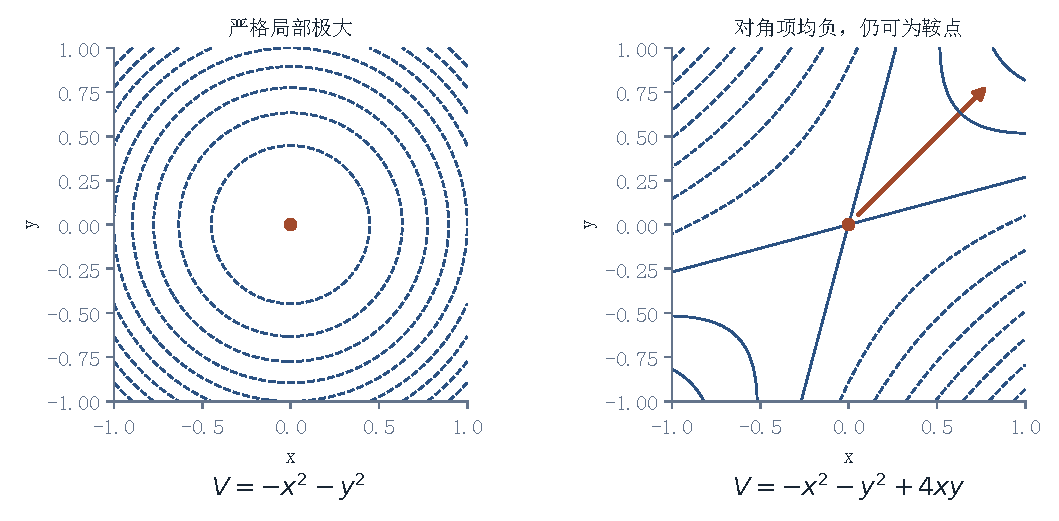
\includegraphics[width=\textwidth]{figures/hessian-directions.pdf}
\caption{两个函数的Hessian对角项均为$-2$。左图为负定，原点是严格局部极大；右图的交叉项使Hessian具有正、负特征值，沿红色方向函数上升，原点成为鞍点。}
\label{fig:mechanism-hessian-directions}
\end{figure}
\subhead{局部最优的三个特征}

停在局部最优上的系统，看上去不像有问题，反而像运行得最好。它可以同时具备三个特征，而这三个特征分别在通常的评价体系里都是正面的。第一是满足度高。系统确实在持续提供用户想要的东西，而且供给效率不断提升。用户的抱怨在减少，因为抱怨的那些点在优化过程中已经被逐条处理掉了。满意度指标好看，留存率好看，增长曲线好看。

第二是稳定。系统不容易被扰动，任何试图改变现状的力量都必须对抗已经形成的整体配置：界面、习惯、商业模式、监管预期、基础设施都已经围绕当前状态调整过，改变一个参数会牵动其他所有参数，成本立刻上升。稳定在这里是一个正面的词，它意味着可预期、可维护、风险低。第三是缺乏生长动力，这一点最难被察觉，因为它不表现为症状。系统没有什么需要解决的问题，也就没有什么需要演化。它的所有改进空间都在当前配置内部：更精细的推荐、更顺滑的交互、更低的延迟。这些改进都在同一条曲线上的平坦区域，边际收益递减，但看起来仍然在进步。

三者叠加的结果是：一个系统可以同时是舒适的、稳定的和停滞的，并且它自己是察觉不到第三项的。这个组合之所以难以纠正，不是因为其中某一项出了问题，而是因为它们互为支撑：正因为满足度高，才没有人有动机去扰动稳定；正因为稳定，才看不到需要解决的问题；正因为看不到问题，改进才会一直沿着平坦区域继续。

\subhead{尼采的末人作为简短对照}

这种处境在思想史上被描述过一次，值得作为对照提出来，但需要把界线划清楚。尼采在《查拉图斯特拉如是说》里写过一个形象，用来描述一种已经放弃了超越的存在：他们不再有渴望，不再有创造，只追求舒适、健康和长寿，并且把这种状态称为幸福。他说这些人“发明了幸福”，然后眨眨眼。\cite{nietzsche1883zarathustra} 这个形象和局部最优的结构有重合，但尼采的批判针对的不是快乐本身，而是当快乐成为唯一目标时，追求更高状态的能力消失了。他的末人不是不幸的，末人恰恰是满足的；问题在于这种满足不再要求任何东西，因此也不产生任何东西。

需要划清的界线在这里。尼采把原因归给价值层面的失败，归给人不再愿意承担更高的目标；局部最优的分析给出的原因更技术化，不是人选择了舒适，而是系统被优化到了舒适的极值点，而在这个点上任何偏离都会立刻降低评价函数的取值。这不是意志问题，是结构问题。人在其中做的每一个决定都可能是理性的，叠加起来却停在一个不再产生新东西的位置上。这个差别的实践含义不小：如果问题是意志，那么解药是呼吁；如果问题是结构，那么解药是改变评价函数本身，而这需要动的是制度、指标和竞争规则，不是个人的决心。

还有一条界线没有划完，而且它比上面那条更要紧。局部最优这个判断本身不含规范内容：系统停在一个极值点上，这件事在结构上是中性的，它是不是失败，取决于评价函数有没有写对。如果评价函数写得正确，那么停在它的最大值上就是成功，不是停滞，而结构分析没有任何工具能把这两种情形分开：它能指出系统不再移动，却指不出这个位置是否值得待。要判定“生长”，必须从结构之外引入一个关于什么算更好的标准，而这个标准不能由同一套优化的语言给出，否则就是循环论证。本章的诊断为停滞准备好了全部机制，没有准备判据；判据是规范问题，不是结构问题，它不能从这里推出来，只能被另外论证。

\subhead{为什么系统不愿离开}

从局部最优离开需要一个特定条件：必须接受一次短期的评价下降，以换取到达另一个更高的局部最优的可能。用形式化的说法，系统需要穿越一段 $V$ 值低于当前水平的地带，这段地带被称为势谷。

\begin{equation}
\Delta V_{\text{escape}} = V(x^*) - \min_{s \in \text{path}} V(s) \ge 0
\label{eq:ch40-escape}
\end{equation}

路径包含起点，因此当前值减去路径最小值非负，表示沿这条路径可能承受的最大暂时评价下降。若要得到到达某个新区域的最小逃逸障碍，还需在允许路径上继续优化。谁承担过渡期的损失、谁获得后续收益，会影响系统是否愿意改变。

个人层面的结构相同，只是承担者换成了自己。一个人要维持某种能力，必须持续使用它，而每一次使用都在当下付出比使用替代方案更高的成本。选择自己写一段文字而不是生成一段，今天的产出更慢、更差；坚持自己去一个地方而不是导航，今天更费时间还可能走错。这些成本是即时的，收益是分散的、延迟的、难以观测的。人的判断系统对即时成本敏感，对延迟收益不敏感，这个偏向在优化充分的低黏滞环境里会被系统性地利用，而且不需要任何人刻意利用它。只要环境提供足够的低摩擦替代品，这个偏向自己就会起作用。

\subhead{停滞不是结局}

把前面的分析收在一起，可以得到一个关于终点的判断。\key{低黏滞陷阱的终点不一定是崩溃，而可能是一个舒适、稳定、缺乏生长动力的局部最优。}系统继续运转，指标继续向好，个体继续得到满足，而整体的可能性空间在收窄。没有人受伤害，没有人抗议，因为确实没有什么可抗议的：系统交付的都是它承诺的东西。收窄发生在另一个维度上，那些需要承受成本才能获得的东西（真实的技能、经过检验的关系、被拒绝过又被坚持下来的判断、一个人自己的边界）不再被生产出来，因为它们的生产过程与当前的评价函数不相容。

这个判断容易被误读成一种文化悲观主义，需要加一句准确的限定。局部最优不是低黏滞环境的必然结果，而是一个需要特定条件才会达到的状态：评价函数必须完全由体验构成，短期反馈必须能够完整地代表长期结果，竞争压力必须有利于最低摩擦方案。当其中某个条件被打破，路径会改变。有大量证据表明现实中的评价函数从来不是完全由体验构成的：身体会出问题，关系会破裂，技能会退化到影响收入，这些长期结果最终会以某种形式回到反馈链上。所以问题不是会不会回来，而是回来的时滞有多长。

时滞决定了代价的分布，也决定了这本书接下来的方向。如果反馈回来的时间很短，个体能在自己的时间尺度上完成校准，代价由自己承担；如果时滞跨越一代人，代价由下一代承担，而承担者没有机会做出不同的选择。这个差别，决定了低黏滞环境是一个可以自我纠正的过程，还是一个只有通过断裂才能纠正的过程。要处理这个问题，需要先看清一件事：人还有哪些能力是系统无法用低成本方式替代的，以及那些能力为什么无法被替代。这个问题在个体身上表现为能力，在群体身上表现为另一种东西：如果大量个体都在同一条路径上适应，那么差异的分布本身也在改变。

\subsection{多样性的丧失与极权心理温床}

前面两节讨论的是个体的边界：拒绝失去对象，系统停在局部最优。这两件事在群体尺度上会合成第三个结果，差异的分布本身发生变化。差异不是抽象的价值，它是边界的原材料。\key{没有差异，就没有可以被拒绝的东西，也没有需要被裁决的冲突。}

\subhead{路径收窄与层流化}

共同的推荐、排序与默认值，可能使许多人暴露于相关的选择路径；用户与网络也可能引入不同方向。群体多样性需要实际测量。流体的层流与湍流不直接给出探索多少、文化好坏或政治倾向的判据，这里的机制应落实到可用替代、共同暴露和纠错能力。

这种收窄的代价已经在别的领域被测量过。金融系统是一个反复出现的例子：同质化程度上升、多样性下降，会让系统更脆弱而不是更鲁棒，当大量机构使用相近的风险模型、持有相近的资产、依赖相近的融资结构时，它们的连接度上升而差异度下降，一个局部冲击因此获得了系统性的放大通道\cite{haldane2011systemic}。农业提供了另一个更早的例子：当一个社会的主粮依赖单一品种时，一次病害就可以穿透整个生产体系，1845 年到 1852 年的爱尔兰马铃薯饥荒属于这一类，单一品种与晚疫病的组合造成约一百万人死亡、约一百万人迁出\cite{ograda1999black}。

这两个例子的共同点不是简化，而是缺少冗余的差异。差异在成本上表现为冗余：多个并行方案、多种做法、看起来多余的选择，都会显得低效。而在扰动到来时，冗余是系统唯一可用的替代路径。低黏滞环境的一个结构性特征，正是它系统性地削掉冗余：既然存在一条最低摩擦的路径，其他路径的使用频率就会下降，最终不再被维护，也不再被练习。

冗余的价值可以用工程上的一个标准来说明。电网运行遵循一条被称为 N-1 的安全准则：系统必须在任何一个元件退出运行之后仍然保持稳定，因此电网必须保有平时看起来多余的容量、备用线路和可调度资源\cite{morison2004power}。这条准则的成本在平时持续发生，收益只在故障时出现，因此它在任何以短期开支为唯一标准的核算里都会被削减。多样性的处境与冗余相同：它表现为成本，兑现为扰动中的存活率，而兑现的时刻在平时看不到。这也是为什么收窄往往不是有人决定收窄，而是没有人有理由为它付账。

这里需要一个重要的边界。把多样性丧失全部归于推荐算法，会错判责任的落点。有研究测量过社交媒体上的跨意识形态接触，结论比流行判断复杂：在 Facebook 的数据中，限制用户接触对立观点的最主要因素是用户自己的朋友构成，算法排序的作用存在，但量级小于前者\cite{bakshy2015exposure}。这个结果的含义不是算法无害，而是收窄有多个来源，把人推向同一路径的力量里，很大一部分来自人自己的选择与网络的同质性。指认正确的机制，是让干预落在有效位置上的前提。

\subhead{秩序的吸引力}

差异被削掉之后，会出现一个看起来无关的心理后果。Arendt的判断在这里可以再往前推一步：她指出极权统治的群众基础是原子化的个体，他们已经失去了阶级、职业共同体和稳定位置的连接；在这样的处境里，孤独比贫困更能解释人们为什么会接受一个把一切事件解释得完全一致的系统\cite{arendt1951origins}。把这个判断与前面两节接起来，可以得到一个更具体的机制：位置消失产生多余感，多余感产生对秩序的需求，而一个持续可用、不犯错、不需要协商的系统，恰好提供了一种廉价的秩序。

这一机制的心理学一侧有可测量的形式。人对自动化系统的信任存在系统性偏差，过度信任与在应当接管时无力接管都会随自动化程度的提高而上升，而这两种失效都不依赖于使用者的知识水平\cite{parasuraman1997humans}。这意味着，交出判断权通常不是一个决定，而是一系列不需要决定的默认：系统给出的答案够用，人工复核显得不必要，几次之后，复核的能力和习惯一起消失。秩序在这里的吸引力不在于它更强，而在于它不需要使用者付出监督成本。

秩序的吸引力还有一层结构原因。一个可解释、可申诉、会出错的秩序，要求使用者承担判断和举证；一个不可解释的秩序把判断收走，同时把责任也收走。对那些已经被判定为多余的个体，交出判断权的收益是双重的：既得到确定性，也免除了为自己判断负责的负担。这也是为什么这种依附很难靠提高警惕来消解，因为它满足的是真实的需求。

依附还有一层更少被提到的收益：它免除了举证的负担。参与一个需要协商的秩序，意味着要说明理由、要面对反驳、要为自己的判断负责；交给一个统一的系统，这些环节全部消失。对那些不确信自己判断能力的人，这种免除是真实的减负，而且它随使用时间增加而加深。这也提示了干预的方向：要维持判断能力，需要的不只是提醒，而是让判断仍然有地方可以提交、有后果可以承担。

把这一步写成必然结局是过度推论。依附的强度取决于替代结构是否存在：如果一个社会仍然保有中间组织，职业共同体、地方关系、长期机构和可以参与的事务，同样的技术压力不会产生同样的依附。技术提供的秩序是可选的，只有当其他秩序来源同时稀薄时，它才成为唯一可得的秩序。分界在这里：不是技术必然导致依附，而是在中间结构被削薄的条件下，依附的成本最低。

三层塌陷到这里合在一处。差异的减少使拒绝失去对象，对象的失去使欲望由外部提供，外部的提供使边界不再由内部维持。这条路径的每一段都在降低下一段的成本，因此它可以被一段接一段地走完，而不需要任何一步是错的。要诊断这条路径，需要的不是道德判断，而是一个能同时容纳三层的结构图。


\begin{figure}[ht]
\centering
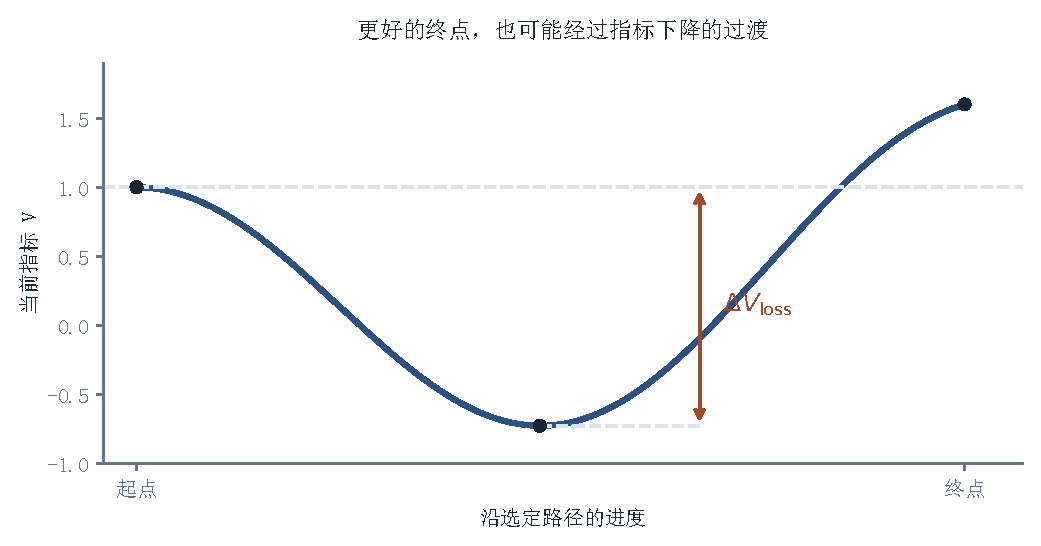
\includegraphics[width=\textwidth]{figures/escape-valley.pdf}
\caption{选定路径上的暂时指标损失。$\Delta V_{\mathrm{loss}}$由起点指标减去该路径上的最小值，因路径包含起点而非负。改变目标、约束或可行路径，会改变这项损失。}
\label{fig:mechanism-escape-valley}
\end{figure}
\section{接回回路：能力、反馈与承责的位置}

三层塌陷可以互相强化。专业位置削弱，使即时认可更有吸引力；很少检验判断的反馈环境，减少了校准的练习；信心下降、替代路径变少，又让人更难回到有效位置。每一条连接都可以调查，每一条连接也都可能成为干预点。

\subsection{三只时钟与几条修复路径}

职业结构可能按年变化，界面可以按周调整，技能、习惯与关系则各有形成周期。成年后的学习与恢复仍然持续。干预需要找准对应过程，及时保住仍可改善的部分。

把进入一种替代体验的成本记为$c_n$，可以写出一个简化递推：
\begin{equation}
c_{n+1}=Gc_n,\qquad G=g_1g_2g_3.
\end{equation}
若三个正乘数都小于1，模型中的进入成本便逐圈下降。这个式子只描述所定义的成本。完整社会回路还需要职业位置、反馈与主体性的独立状态变量，以及延迟、外部输入和可观察的因果连接。

\begin{figure}[ht]
\centering
% >>>>>>>>>> figs/fig-collapse-cycle.tex >>>>>>>>>>
% 图 5-3  三级下沉的回路结构
% (a) 三节点回路：功能层 → 真实层 → 主体层 → 功能层，三条弧上各带一个削减比例
%     $g_i$，环心给出传递关系。节点第二个小字是各层的时间尺度。
%     $g_i=1$ 表示该层不再以更低的门槛把代价传给下一层。
% (b) 门槛 $c_n$ 随圈数的下降：$c_n=G^n$，对数纵轴。三条线对应 G=0.5 / 0.8 / 1.0，
%     说明「取消一节只是放慢、三节都取消才停住」。
% 与图 5.1 的分工：那张画的是三层之间的**链**（谁把谁推向哪里），
% 这张画的是那条链首尾相接之后的**回路**与其传递系数，正文明确区分过这两者。
%
% 版心宽 144mm，这张图按 \useasboundingbox 算到 138mm——第一版画到 149mm，
% 编译时在 \end{tikzpicture} 处报 14.2pt overfull。盒子从 2.60 收到 2.30、
% (b) 的横轴从 0.58/格 收到 0.50/格之后才装得下。改之前先量总宽。
\begin{tikzpicture}[x=1cm, y=1cm, font=\small,
  bn/.style={draw, line width=0.7pt, rounded corners=2pt,
             minimum width=2.30cm, minimum height=0.94cm, align=center,
             inner sep=2pt, text=ink},
  gl/.style={font=\small, text=ink, inner sep=1pt},
  ax/.style={-{Stealth[length=2.0mm]}, ink, line width=0.6pt},
  tick/.style={font=\scriptsize, text=slate}
]
\useasboundingbox (-0.85,-0.50) rectangle (12.95,-7.30);

% ================= (a) 三节点回路 =================
\node[bn, draw=terra!60, fill=terra!13] (f) at (3.30,-1.30)
      {功能层\\[0.5pt]{\scriptsize\color{slate}年}};
\node[bn, draw=rust!60,  fill=rust!13]  (r) at (6.10,-5.70)
      {真实层\\[0.5pt]{\scriptsize\color{slate}月—年}};
\node[bn, draw=forest!60, fill=forest!13] (s) at (0.50,-5.70)
      {主体层\\[0.5pt]{\scriptsize\color{slate}代}};

% 顺时针三边：功能层→真实层→主体层→功能层
\draw[-{Stealth[length=2.2mm]}, slate!70, line width=0.9pt] (f) -- (r);
\draw[-{Stealth[length=2.2mm]}, slate!70, line width=0.9pt] (r) -- (s);
\draw[-{Stealth[length=2.2mm]}, slate!70, line width=0.9pt] (s) -- (f);

% 环心的传递关系。分两行写：单行放不进三角形内空（内空最窄处约 3.4cm）。
\node[font=\small, text=ink] at (3.30,-3.95) {$c_{n+1}=G\,c_n$};
\node[font=\small, text=ink] at (3.30,-4.34) {$G=g_1g_2g_3<1$};

% 三个削减比例，放在各边外侧（沿外法向偏移 0.45cm，已核对仍在三角形之外）
\node[gl] at (5.08,-3.26) {$g_1$};
\node[gl] at (3.30,-6.22) {$g_2$};
\node[gl] at (1.52,-3.26) {$g_3$};

% ================= (b) 门槛随圈数下降 =================
% \bx 不能再小：纵轴刻度字「0.01」以轴心右对齐，左端伸到轴外约 0.75cm，
% 8.45 时它的左端在 7.62，正好让开真实层盒子的右缘 7.25。
\def\bx{8.45} \def\bdx{0.50} \def\byB{-6.16} \def\bah{4.20}
\def\yy#1{\byB+\bah*(log10(#1)+2)/2}   % c=1 在上端，c=0.01 在下端，两个数量级

\draw[ax] (\bx,\byB) -- ({\bx+\bdx*6+0.42},\byB)
      node[anchor=west, font=\scriptsize, text=ink] {$n$};
\draw[ax] (\bx,\byB) -- (\bx,{\byB+\bah+0.30})
      node[anchor=south, font=\scriptsize, text=ink] {$c_n$};

% 纵轴刻度：1 / 0.1 / 0.01。只标这三条，其余留给曲线。
\foreach \c in {1,0.1,0.01} {
  \draw[slate!55, line width=0.45pt] ({\bx-0.07},{\yy{\c}}) -- ({\bx+0.07},{\yy{\c}});
  \node[tick, anchor=east] at ({\bx-0.13},{\yy{\c}}) {\c};
}
% 横轴刻度：圈数 0--6
\foreach \k in {0,...,6} {
  \draw[slate!55, line width=0.45pt] ({\bx+\bdx*\k},{\byB-0.07}) -- ({\bx+\bdx*\k},{\byB+0.07});
  \node[tick, anchor=north] at ({\bx+\bdx*\k},{\byB-0.12}) {\k};
}

% 三条 c_n=G^n。G 越大下降越慢，G=1 是一条水平线。
% 先画陡的，最后画平的，免得被压在下面。
\foreach \G/\cl in {0.50/rust, 0.80/terra, 1.00/forest} {
  \draw[\cl, line width=1.3pt]
    \foreach \k in {0,...,5} {
      ({\bx+\bdx*\k},{\yy{pow(\G,\k)}})
      -- ({\bx+\bdx*(\k+1)},{\yy{pow(\G,\k+1)}})
    };
}

% 曲线右端的标签。纵坐标由同一式子算出，不手填，免得改了曲线忘了改标签。
\pgfmathsetmacro\yA{\yy{1.0}}
\pgfmathsetmacro\yB{\yy{0.8^6}}
\pgfmathsetmacro\yC{\yy{0.5^6}}
\node[anchor=west, font=\scriptsize, text=forest] at ({\bx+\bdx*6+0.14},\yA) {$G=1$};
\node[anchor=west, font=\scriptsize, text=terra]  at ({\bx+\bdx*6+0.14},\yB) {$G=0.8$};
\node[anchor=west, font=\scriptsize, text=rust]   at ({\bx+\bdx*6+0.14},\yC) {$G=0.5$};

% ================= 栏标题（一律在内容下方）=================
\node[anchor=north, font=\footnotesize\heiti, text=slate] at (3.30,-6.72) {(a) 三层的回路};
\node[anchor=north, font=\footnotesize\heiti, text=slate] at (9.95,-6.72) {(b) 门槛的逐圈下降};
\end{tikzpicture}

% <<<<<<<<<< figs/fig-collapse-cycle.tex <<<<<<<<<<

\caption{进入成本的简化递推。假设三个正成本乘数固定且均小于1，乘积决定成本曲线的下降速度。图示说明这个成本模型，不代表职业、反馈与主体性的完整因果动力学；真实干预还可改变乘数、结构与外部输入。}
\label{fig:collapse-cycle}
\end{figure}

调查可以先从较窄的问题开始：进入一项职业是否更难？辅助工具改善了独立测试的技能，还是只提高即时产出？使用者能否识别、质疑并纠正一次重要错误？申诉是否改变决定？替代路径是否负担得起、实际可用？

这些问题需要不同证据：纵向观察、任务测试、机构记录与具体案例。指标还要接受反向检查，避免把“记录了多少次申诉”误当成“解决了多少问题”。恢复机制需要有实际改变过程的能力。

\subsection{承责结构的四项功能}

后果需要一条进入回应的路径。承责结构至少要提供四项功能。

\textbf{发现。}监测损害、险情与重要偏离；让使用者和受影响者能够报告问题。运营方的仪表盘与外部投诉入口要能够相接。

\textbf{追溯。}把事件接回相关决定、版本、配置与工具行动。记录的范围、保存期限、访问权限与隐私保护，需要随用途一起设计。

\textbf{止损。}让某个位置拥有实际可用的暂停、隔离、召回或限制权。紧急控制可以先于完整归因，避免调查期间继续扩大损害。

\textbf{救济。}让受影响者能够要求纠错、获得适当补偿，并推动防止复发。责任背后的资产、保险与组织能力，决定了承诺能兑现多少。

\begin{figure}[ht]
\centering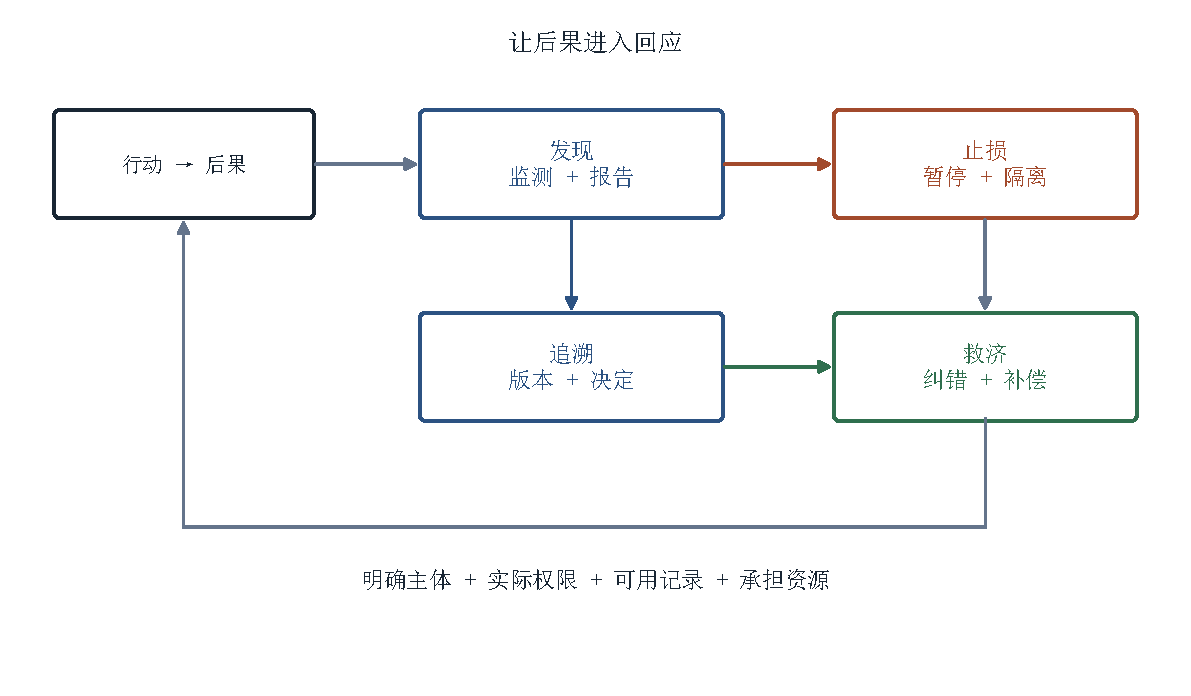
\includegraphics[width=\textwidth]{figures/accountability.pdf}
\caption{承责的四项功能。监测和报告使后果进入记录，追溯提供解释与纠错依据；止损可以立即启动，救济继续处理已发生的后果。四项功能相互连接，并可并行运行。}
\label{fig:accountability-loop}
\end{figure}

四项功能可以并行，也会互相提供输入。每一项都需要主体、资源与操作接口。航空业把设计保证、生产控制、维护、运行权限、报告与调查组织在一起，可靠性由航空器和制度共同形成。其他领域也需要根据自己的后果与控制条件安排这些功能。

机器系统的接口需要同样清楚：谁控制更新，谁能暂停访问，服务停运后哪些记录仍在，谁受理对模型决定的异议，谁有能力承担救济？

责任可以依据控制能力、合同角色、法定义务与其他正当标准分配。保险与补偿基金能够分担部分损失，独立调查有助于把学习与即时归责区分开。激励、执行和资金共同决定这些安排是否真正工作。

承责也能扩大部署。风险具有明确控制、记录和救济路径，就更容易被评估和采用。系统知道不确定性变成后果时如何行动，一部分原本难以承诺的应用才获得可运行条件。

\subsection{判断需要资格}

三个问题始终留在决定的核心：哪些后果可以接受，多少证据足以行动，谁有权把代价施加给谁。

模型可以估计结果、比较方案、揭示矛盾，也能帮助人表达立场。采用标准与施加后果，还需要相应权利、授权和职责。本书主张：\key{承担后果的人，应当保有有效发言、代表与质疑的渠道。}

直接暴露构成一种资格来源；合法委托、专业义务、民主授权，以及对缺席者和弱势者的保护，也构成资格来源。患者承担身体风险，医师承担专业责任，两种位置通过知情同意、专业标准与追责程序连接起来。陪审员通常不承受被告同样的后果，其权限来自法律赋予的角色、义务与程序。\cite{kalven1966american}

机长、医师、陪审员各有不同依据。共同要求是：决定有可说明的理由，权限有明确范围，受到质疑时有人必须回应。复核者还要具备能力、时间和改变决定的权力，纸面的“人在回路”才会成为实际位置。

\subsection{产出变便宜，人的价值如何成立}

只按稀缺产出衡量人的社会，会在产出变丰裕时失去一部分价值尺度。参与、照护、关系、判断与有限生命，需要进入更完整的评价。

后果落在某个人身上，使这个人获得保护与发言的理由。负担如何分配，还要依照正当的权力和控制关系来判断。承担本身无须被浪漫化，能够减少的伤害应当减少。

另一个人可以提供建议、劳动或受托决定，却不能因此替你活完同一段有限生命，也不能自动占据同一关系。辅助扩大一个人的能力，这个人在结果中的利害仍然存在。

修复的方向因此很具体：重建进入有用贡献的路径，保留能够纠错的反馈，让退出、异议和长期承诺继续可行，把有后果的行动接回能够回应的人与机构。它们需要投入。下一章继续区分：哪些成本只是在阻挡，哪些成本维护了进步值得拥有的条件。

\furtherreading{%
Hannah Arendt，\textit{The Origins of Totalitarianism}\\
Herbert Marcuse，\textit{One-Dimensional Man}\\
Jean Baudrillard，\textit{Simulacra and Simulation}\\
René Girard，\textit{Deceit, Desire, and the Novel}\\
Harry Kalven Jr.\ \& Hans Zeisel，\textit{The American Jury}\\
Ivan Illich，\textit{Tools for Conviviality}\\
Cathy O’Neil，\textit{Weapons of Math Destruction}\\
Theodore Kaczynski，\textit{Industrial Society and Its Future}}


% <<<<<<<<<< parts/book-ch05.tex <<<<<<<<<<


% >>>>>>>>>> parts/book-ch06.tex >>>>>>>>>>
%% ===================== 本章参考文献 =====================
\printbibliography[heading=subbibliography,title=参考文献]

\chapter{价值的重构：在剪切带中栖息}

上一章说明了后果需要被接住，也说明了承受者与决定者可能分离。价值重新分布到哪里，还取决于需求、产权、议价与公共安排。本章区分三件事：某项工作的社会必要性，承担它的人获得的报酬与地位，以及人的尊严和生活意义。三者会互相影响，却没有自动兑现的关系。生成能力充足之后，验证、照护、长期关系与责任可能更加稀缺；这些位置能否获得资源，需要回到制度和分配。历史上的能力外化，提供了考察这种变化的几组材料。

如果智能系统已经能写文案、做总结、翻译、修图、写代码、做方案，普通人的技能还剩下多少重量？如果它还能读文献、提假说、设计实验、跑模拟、分析数据、写论文，科研训练又该如何证明自己的价值？如果它进一步参与数学证明、搜索引理、检查推导，科研中最硬的形式智力劳动是否也开始松动？如果机器人会驾驶、制造、搬运、巡检、手术和照护，那些过去依赖身体、经验和现场判断的工作，还能保留多少人的位置？问题不是某些职业会不会被替代，而是过去用于证明人的训练、经验和主体资格的能力接口，正在被外部系统拆开。

这些问题表面上是在问职业会不会消失，技能会不会贬值，实际上是在问一种更深的东西：过去，人用什么证明自己有价值。会写、会算、会做、会判断、会研究、会证明、会行动，曾经都能支撑一个人在社会中的位置。现在，这些能力正在被外部系统一层层取走、放大、重组。真正让人不安的，不是机器到底还有什么永远做不到，而是当一种能力被外化之后，人该迁移到哪里。

\section{历史的回响：价值漂移的物理学}

这些问题不是第一次被问，答案也不是第一次被改写。第一章已经给出过那条判断：技术每一次外化一种能力，都会切断能力与价值之间的旧绑定，因为被外化的从来不是某一项孤立能力，而是旧社会用来识别训练、经验、资格和责任的接口。这一章要接着往下问的是被切断之后的事：价值落到了哪里，以及它为什么落在那里。三种证明的失效是同时发生的：产出不再天然证明主体，形式不再天然证明经验，能力不再天然证明正当性。把它们拆开可以看到，三者各自依赖一个可以被外部系统接管的环节，而迁移的方向正是由这些环节的位置决定的。

这里说的接口不是抽象说法，它对应一组具体的制度安排。行会用学徒年限确认手艺，科举用考试内容确认资格，大学用文凭确认训练，职业执照用考试和实习期确认准入，学术共同体用发表记录确认可信度。这些安排的共同点是它们把能力的证明落在一个人无法快速获取的过程上：七年学徒期不能压缩成七个月的阅读，住院医师的病例数不能由考试成绩替代，论文的同行评价不能由作者自述替代。接口的作用正是把这种无法快速获取的过程固定成可识别的形式，因此它一旦被外部系统接管，失去的不只是能力的稀缺，还有确认资格的整套程序。\cite{spence1973job}

历史给出的答案从来不是“人不再有价值”，而是价值换了一个挂靠点。这个过程可以沿着几个节点看清：能力被移走的方式不同，旧绑定断裂的方式也不同，而每一次断裂都留下一个相同的问题：被释放出来的那部分价值，接下来要落在哪里。理解这条线不需要完整的技术史，只需要每个节点上最硬的那一步。

\subsection{苏格拉底的恐惧：当智慧失去内化的黏滞}

\subhead{能力外化与旧绑定的断裂}

这里不是要写一部完整技术史，而是抓住几个能力外化的关键节点：记忆、复制、时间刻度、做功、规则执行、符号生成、形式探索、行动能力和生命干预。人类不是第一次经历这种失重。文字让记忆变轻，印刷术让复制变轻，钟表让时间变轻，蒸汽机让肌肉变轻，计算机让规则执行变轻，大模型让符号生成变轻，推理模型和科学代理体让形式探索变轻，具身智能让行动能力开始外化，生命智能让生命干预和生命定义进入技术系统。每一次技术都像一次深层搬迁：它把原本沉积在身体、技艺和身份中的能力移到外部系统里，使旧的价值接口突然松动。但人的价值没有因此消失，而是被迫迁移到更深、更重、更难外包的位置。这九个节点排在一起，是一条价值落点被反复重排的线；重排的结果由谁获得，不取决于技术本身。

节点的顺序不是随意的，它对应抵抗被形式化的能力级别。记忆最先被移走，因为一段话可以被写下来；复制随后被移走，因为一次抄写可以被压成版式；做功被移走得晚一些，因为肌肉必须真的克服重力；规则执行、符号生成、形式探索依次被移走，因为它们分别能被写成流程、写成统计规律、写成可搜索的空间。越是能被写成外部形式的能力，越早离开身体。这个顺序解释了为什么每一次外化都会先打击那些把能力当作身份的人：他们的位置建立在“我能做到别人做不到的事”上，而外部系统恰好把这件事变成了一件便宜的事。

断开的旧绑定有固定的内容。它包含训练的可验证性（这个人确实经过了长时间的准备）、经验的可追溯性（他见过这类对象，并且记得后果）、资格的排他性（不是所有人都能进入这个位置）、责任的归属（出了问题由他承担）。四件事在旧制度里是捆在一起的，一个能力同时证明四件事。外化切断的是捆绳：训练可以外包给模型，经验可以由检索替代，资格可以由订阅获得，责任则在系统之间分散。断口出现的位置，就是价值必须重新落户的位置。

\subhead{记忆的外化与内化的黏滞}

第一个节点是记忆，它外化的时间最早，也最彻底。文字发明以前，记忆不是普通能力，而是秩序本身。法律、神话、谱系、祭祀、交易、禁忌和经验，都必须依赖人的身体保存。能记住、能复述、能传承的人，不只是信息容器，也是共同体时间的承载者。遗忘不是个人失误，而是秩序断裂。文字改变了这一点。它让经验第一次稳定地脱离身体，沉积在符号中。人会死，声音会消失，亲历者会离场，但话语、契约、律令、诗歌、账目和知识可以留下。柏拉图在《斐德若》中借苏格拉底之口警惕文字：它像记忆的药，也可能让人误把外部保存当成内部理解。\cite{plato_phaedrus} 这不是简单反技术，而是看见了第一次\term{价值迁移}：记忆变轻以后，理解变重；文本可以固定答案，却不能替代追问；一个人可以拥有一段话，却未必拥有这段话背后的判断。

苏格拉底的恐惧有一个准确的落点：知识从大脑的生物神经迁移到羊皮卷之后，人对知识的体感不再随文字一起传递。背诵在这里不是低级的存储，而是把内容反复穿过身体、与经验咬合在一起的内化过程，它的黏滞很高，也很贵。文字把这份黏滞降到接近于零，于是“能记住”不再稀缺，稀缺的是“能推演”。文字没有摧毁智慧，它只是换掉了智慧的支点：价值从存储漂移到逻辑构建，从知识的容器漂移到知识的处理器。这场迁移在公元前四世纪就已经完成一半，它留下的问题一直没变：外部保存可以固定答案，却无法替人完成理解。

口传社会的研究给这场迁移提供了一个可以直接测量的对照。Milman Parry 和 Albert Lord 在二十世纪三十年代记录南斯拉夫的口传史诗歌手，发现优秀的歌手并不是把上万行诗句背下来，而是掌握一套格律套语，每次演唱都在现场重新组装；同一位歌手在不同场合唱同一部史诗，长度可以相差几千行。\cite{parry1960singer} 记忆在这种条件下不是仓库，而是一种持续施工的能力，它同时承担着创作、传承和校验。文字把这三件事拆开了：创作归作者，传承归抄本，校验归后来的读者。拆开之后，记忆作为整体能力的黏滞消失了，而理解、校订与解释的黏滞上升了，这也是苏格拉底看到的那一层变化。

这里需要留一个反向的限定，否则这个判断会被读成“文字使人变浅”。书写不只保存了已有的思想，它还制造了新的思想对象。位值制记数和代数符号让运算可以在纸面上一步步展开，证明可以脱离讲述者的记忆被检查，几何作图可以被后人重新走一遍。文本把推理从人脑中搬出来，使它可以被他人停顿、质疑和改写，这件事本身就是推演能力的一次扩张，而不只是记忆能力的一次损失。内化的黏滞被降低，换来的是可公共检查的形式，代价与收益同时成立。

记忆外包之后会发生什么，现代的对照实验给出了一个可以测量的答案。Sparrow、Liu 和 Wegner 在 2011 年发表的一系列实验显示，当被试预期某条信息可以在以后被检索到，他们对这条信息本身的记忆成绩下降，而对“这条信息存在哪里”的记忆成绩上升，研究者把这个现象称为谷歌效应。\cite{sparrow2011google} 这个结果需要按它实际测量的东西来读：它测到的是记忆内容的分布发生了变化，不是记忆能力的净损失，实验也不能说明外部保存一定有害。考试制度的调整提供了一句旁证：允许检索的开卷考试不再考察记忆，转而考察组织、判断与表达，而闭卷考试至今仍在大量场景中使用，理由并不是记忆本身值得尊敬，而是某些领域里的判断必须以足够的内部知识为前提。两份证据指向同一个结构：外化改变的是稀缺的位置，不是人的总量。

记忆变轻只是第一次，复制变轻的幅度更大，而它动的不是个人的理解力，是权威本身。当文本可以被大量复制，谁有权解释文本就取代了谁拥有文本，成为新的稀缺位置。这是一次和记忆完全不同的迁移：前一次迁移发生在个人的能力结构里，这一次迁移发生在共同体的权力结构里。

\subsection{古腾堡的降维：解释权垄断的黏滞坍缩}

\subhead{复制的降维与解释权的坍缩}

印刷术进一步降低了复制的重量。手抄时代，文本本身稀缺，拥有书、抄写书、保存书，就是权力。印刷术让文本大量扩散，使知识从少数空间中涌出，进入更广阔的社会循环。Eisenstein 把印刷术视为近代欧洲知识秩序转变的重要力量，因为它改变的不只是复制速度，也包括校勘、传播、争论和权威形成方式。\cite{eisenstein1979printing} 可是复制变轻以后，人的价值没有消失，而是从复制迁移到筛选、解释、校订、组织信任和建立公共判断。文本越多，判断越稀缺；复制越便宜，信任越昂贵。印刷没有让人无关，反而让“谁解释、谁校验、谁建立可信版本”变得更重要。

这一步降维的对象不是文字，而是复制本身。手抄受制于抄写员的物理速度，一位抄写员一天能完成的字数有限，经文因此稀缺，解释权因此可以被垄断在少数人手里：谁掌握抄本，谁就掌握通往真理的入口。当复制的边际成本趋近于零，信息以接近超流体的方式扩散，稀缺的位置从经文转移到诠释，1517 年马丁·路德把《九十五条论纲》送上印刷机，几年之内传遍欧洲，靠的不是教会的准许，而是复制已经不再昂贵。诠释随即通胀，旧权威在低黏滞环境里失去支点，恐慌的本质不是信息过载，而是解释权换了主人。价值也从“拥有信息”漂移到“定义信仰”，再漂移到为信息建立可信版本，这条漂移线在往后的每一次外化里都会重演。

复制的降维还有一个不显眼的后果：它让校勘和版本比对第一次成为可以规模化的技术工作。同一部书的不同版本可以被并排比较，异文可以被系统整理，错误可以在重印中修正，作者可以在生前反复修订自己的著作。这些工作在过去依赖少数抄写室的传统，后来变成出版机构、图书馆和学术团体的常规职能。复制变便宜的同时，确认哪一个版本可信的成本上升了，于是新的位置出现在校订者、编纂者和出版者一边。稀缺没有消失，它只是从“有没有文本”换到了“文本是否可信”。

复制和生成变便宜，既可能扩展知识，也会增加筛选与建立可信版本的需求。确认本身也可以被工具加速。需要观察的是整条链上哪种功能相对稀缺，以及承担这项功能的组织能否得到资源。

\subhead{规则执行与符号生成}

复制变轻以后，被移走的能力不再停留在复制一侧，而是转向了可被写成流程的那部分心智劳动。规则的重量无法用吨和瓦特计量，迁移的结构却相同。计算机又把这种迁移推进到心智劳动。它降低的不是全部思考，而是可形式化、可规则化、可程序化过程的成本。手算、账务、表格、数据存储、检索、排序、重复执行和确定性流程，被机器大规模吸收。一个人算得再快，也不可能以这种方式重新赢回价值。于是人的位置迁移到更上游：定义问题，建立模型，选择变量，理解语境，判断输出是否对应现实需求。计算机让执行变轻，却让问题定义变重。Simon 讨论人工物和有限理性时已经指出，人的智能并不是脱离环境的纯粹求解，而是在目标、约束、信息和组织结构中设计可行路径。\cite{simon1969sciences} 当执行被外包，真正稀缺的不是执行本身，而是知道什么值得执行、为什么执行、哪些问题可以形式化、模型边界在哪里、结果是否应该进入现实。

会计行业在几十年里完成过一次完整的演示。手工记账、试算平衡、报表汇总这些环节被电子表格和财务软件吸收之后，记账员的数量下降了，但审计、税务筹划、内部控制和财务解释的位置没有减少，反而因为数据量变大而增加。变化不在于工作量，而在于能力证明的方向：能把账做平不再证明什么，能判断一笔交易应该如何被处理、能否经得起事后检查，才构成资格。这条路径和计算机在其他确定性流程密集行业里造成的路径一致，只是它发生得更早，也更容易观察。

大模型的冲击更深，因为它进入了人最习惯用来证明自己的区域：语言、表达、解释、代码、证明、方案、风格、总结、计划和初级判断。蒸汽机替代肌肉，计算机替代规则执行，大模型则开始替代大量符号产出。它不是一个更聪明的写作工具，而是文字之后最重要的符号事件之一。文字让经验脱离身体，印刷让经验大规模复制，计算机让符号按规则执行，大模型让已经外化的人类经验重新组合、回应、生成和代理化。外部记忆不再只是保存和等待检索，它开始主动说话、主动解释、主动计划、主动调用工具。

这个变化已经超出“模型能答题、写代码、过考试”的阶段。GPT-5.5 的系统卡把它定位到复杂现实工作，包括写代码、在线研究、分析信息、创建文档和表格，并在多工具环境中推进任务。\cite{openai2026gpt55systemcard} o3 和 o4-mini 的系统卡则把推理模型与网页浏览、Python、图像和文件分析、自动化、文件搜索和记忆等工具能力结合起来。\cite{openai2025o3o4minisystemcard} Deep Research 和 ChatGPT Agent 进一步说明，研究、检索、网页交互、代码运行、数据分析和文件生成正在合流。\cite{openai2025deepresearchsystemcard,openai2025chatgptagentsystemcard} 这些系统共同指向一个趋势：大模型正在从符号生成器转向工具化、代理化的任务系统。人的价值问题也因此不能停留在“谁写得更好”。如果模型能写、能查、能算、能跑代码、能调用工具、能生成报告，那么人的价值必须迁移到更深的位置：谁确认信息，谁定义问题，谁判断结果可以进入现实，谁接管失败，谁承担后果。

但镜子不是世界。大模型可以生成知识的外形，却不自动拥有经验；可以生成证明的外形，却未必真正穿过规则；可以生成关怀的外形，却没有承受关系；可以生成行动方案，却没有接触后果。过去，一段判断通常暗示背后有某个说话者、某段经历、某种责任；现在，形式可以在没有经历、没有验证、没有承受的情况下大量出现。形式和经验之间的旧联系被削弱了。大模型让文明的外部记忆会说话，也让“说出来”本身失去原有重量。

\subhead{生成之后的验证序列}

外部记忆开始说话之后，价值的位置需要重新安排。验证可以按介质差异分成形式、语义、因果、工程、生命长期和社会责任六层，那是按对象分类；换一个角度，按后果的深度排列，同一条链可以读成一个逐级上升的序列，每一级都比上一级更慢、更贵、更不容易被替换。候选与凭据之间的距离，正是价值要重新沉淀的地方。

所以，大模型之后，人的第一层价值不是继续生产更多符号，而是让符号重新接回现实。生成越便宜，验证越稀缺；候选越多，判断越重要。答案不是知识，解释不是理解，方案不是行动，模拟不是后果。智能时代不是知识自然变多，而是候选爆炸。只有穿过验证金字塔的候选，才可能成为可依赖的结果。这里所谓价值，不只是劳动市场中的交换价值，也包括知识共同体中的可信性、制度系统中的授权性，以及关系和生命世界中的承受性。AI 可以降低产出的成本，却不会自动生成这些价值的正当性。

这座金字塔的层级并不复杂：候选生成 $\to$ 表征确认 $\to$ 推演确认 $\to$ 行动确认 $\to$ 系统嵌入 $\to$ 长期承受。候选生成回答“能不能说出来”；表征确认回答“对象是否存在、来源是否可靠”；推演确认回答“证明、代码、计算和因果链是否成立”；行动确认回答“能否进入真实环境，错误能否停止、回滚和追责”；系统嵌入回答“组织、平台、医院、道路、工厂和制度能否接住”；长期承受回答“能否经受时间、规模、异常、滥用和代际后果的检验”。智能系统当然也可以参与验证，甚至在许多局部环节上比人更稳定；但这只说明部分验证也会被外化，并不意味着验证的正当性自动完成。智能可以生成判断，也可以验证判断，却不能自动授予判断进入现实的正当性。

链条一旦展开，就能看出各段的迁移速度并不一样。越靠前的环节越容易被自动化替代，因为它的输入和输出都可以被表述清楚；越靠后的环节越慢，因为它的判据要在时间中才能获得，而且判据的持有者必须自己承担判断错误的代价。科研同时包含最硬的形式环节和最重的对象环节，先变的是前一半，这不是因为后一半更复杂，而是因为后一半的判据不在系统内部。这一层区别，把下一步的讨论推向了两端：规则空间里的搜索，和真实对象上的接触。

\subsection{钟表与蒸汽机：被规训的时间与被解放的肌肉}

\subhead{钟表先规训了时间}

在蒸汽机之前，机械钟表已经先动过一次手，它外化的不是肌肉，而是时间。自然节律下的工作随日升日落展开，小时是模糊的，赶工看天色和季节，人对节奏保留着相当大的自主。钟楼和怀表把时间切成均匀、可计量、可分割的刻度，工厂汽笛把刻度变成纪律，准时成为美德，迟到成为过失，效率第一次可以被计时比较。这一层外化不产出任何实物，却重排了所有人的生活，工业秩序的地基因此不是煤和铁，而是被规定的时间；人在这里失去的不是力气，而是对节奏的支配。

蒸汽机改变的不是符号，而是能量。它让人和动物的肌肉不再是主要动力来源。过去，体力、耐力、速度和直接做功能支撑大量社会位置；蒸汽机之后，力量开始沉积在机器、燃料、铁路、工厂、城市和资本中。人的身体不再是做功的核心单元，社会开始围绕机器功率重组。旧手艺失重，旧劳动被重新纪律化，但人没有消失。人的价值从肌肉迁移到控制、组织、维护、调度和责任。机器越有力量，事故越严重；功率越大，标准、维修、培训、调度、保险和责任越重要。工业革命不是简单让人从劳动中解放出来，而是让身体做功失去旧价值，把人的位置推向机器系统的设计、管理、协调和承责。\cite{landes1969unbound}

钟表和蒸汽机合起来完成的是同一次迁移：人从做功者变成控制者，价值锚点从克服物理阻力漂移到管理复杂系统。控制者的位置比做功者的位置更抽象，它要求的是把机器、时刻表和陌生人组织起来的能力，因此也更难被一次技术升级抹掉。这几层外化有一个共同点，被移走的能力都在外部世界里留下了可见的、可计量的载体，因此旧的位置还能被重新找到。机器开始吸收规则、符号和形式探索之后，迁移的方向就不再这么直观。

\subsection{被外化的形式与行动}

\subhead{形式探索的外化}

科研也会因此重新定位，其中数学和理论研究只是最尖锐的一端。这里需要区分三个层级：符号生成是说出形式，形式探索是在规则空间中产生新结构，验证则是让新结构被规则、共同体或现实对象接住。过去，能写出证明、能提出构造、能搜索算法，本身就是高强度训练的证明；现在，这些接口也开始松动。AlphaGeometry 在奥林匹克几何问题中把神经生成与符号演绎结合起来：神经模型提出辅助构造，符号引擎负责推演和检查，在无人工示范的情况下合成大量几何定理与证明。\cite{trinh2024alphageometry} 这个例子说明，可靠证明不是“像证明的文字”，而是形式生成与规则确认的结合。

更强的信号出现在 2026 年：OpenAI 模型给出反例，推翻了与 Erdős 1946 年平面单位距离问题相关的核心猜想方向；随后 Alon、Bloom、Gowers、Litt、Sawin、Shankar、Tsimerman、Wang 和 Wood 给出一份短的、消化过的、人类验证版本，并对结果进行反思。\cite{openai2026unitdistancedisproof,alon2026remarks} 这里必须说得精确：这不是说单位距离问题已经被一句话“解决”，也不是说数学共同体可以被省略；它说明，连最硬的形式智力接口也开始松动。模型能够提出真正改变问题图像的构造，但这个构造要成为数学知识，仍然需要人类数学家检查、压缩、解释、命名和嵌入理论。

AlphaEvolve 展示了另一种形式探索外化方式。它不是简单让模型写一段证明，而是把大模型生成、代码修改、自动评估和演化搜索结合起来，使候选算法在反馈中迭代改进。白皮书称，它在若干数学、计算和基础设施优化问题中产生了有用结果；其中最适合作为例子的，是它在 4$\times$4 复矩阵乘法这一特定设置中找到使用 48 次标量乘法的程序，改进了长期未被突破的结果。\cite{novikov2025alphaevolve} 这个案例不应被泛化成“AI 已经解决算法发现”，它更准确地说明：在可形式化、可评估、可迭代的搜索空间里，候选生成和候选筛选可以被机器闭环加速。人的价值因此不是消失，而是迁移到对问题、评价函数、验证标准和共同体准入的判断上：什么问题值得搜索，评价器是否正确，候选是否只是过拟合评估器，结果是否可解释、可证明、可迁移、可进入知识体系。这类外化之所以还停在形式一侧，是因为评价器本身可以被写成代码；一旦评价必须由对象给出，迁移就会换一种形态。

\subhead{前沿难题中的构造与确认}

上面两个案例合起来指向一个更大的问题：形式探索的外化能推到多硬的问题上。数学中被单独标出的那一组难题（黎曼猜想、Birch 和 Swinnerton-Dyer 猜想、纳维-斯托克斯方程解的存在性与光滑性一类）有特殊地位，不只因为难，而因为它们的判定标准极其干净：命题要么被证明，要么被推翻，中间没有解释空间，也没有行业惯例可以商量。任何外部系统如果在这类问题上产生实质推进，它碰到的是本书全书讨论的那条最硬的线。

按介质响应谱的说法，这里要问的是阻抗匹配：同一束智能输入进入数学，与进入实验科学，被吸收的方式完全不同。数学一侧的阻抗低，因为它的验证器是形式化的，一个候选对象只要合法就能被独立检查；实验一侧的阻抗高，因为验证器是对象本身，而对象不接受任何形式的替代。这个差别解释了为什么形式探索会先在这一侧松动，也解释了为什么它的松动不能外推。

同一个图像在二〇二六年由陶哲轩以另一套词汇独立提出，而它出现的位置比第三章更靠内。第三章的失配发生在智能输出与外部介质之间，源端是模型，负载端是原子、生命或组织；这里的两端都在知识生产的内部，源端是生成，负载端是消化。他把数学工作拆成生成、验证、消化三件事，消化指的是理解一个结果、把它放进上下文、把它讲清楚。历史上三者的难度相当，消化作为副产品自然发生，因此共同体奖励的是生成与验证。生成能力提高之后，三者的速率分开了：生成最快，验证因为形式化也跟着加快了一部分，消化几乎没有变快。他把这个分离直接称为阻抗失配，并说数学正从证明稀缺进入证明过剩，而它的文化和基础设施还没有适应这个转变。\cite{tao2026aiviews}

生成与消化的分离，先表现为两种能力的比值。设$g>0$为单位时间新增候选的数量，$d$为同一口径下可供消化的能力，能力覆盖比记为
\begin{equation}
\begin{split}
\rho&=\min\!\left\{1,\frac{d}{g}\right\},\\
\left.\frac{\mathrm{d}\rho}{\mathrm{d}t}\right|_{0<d/g<1}&<0
\quad\Longleftrightarrow\quad
\frac{\dot g}{g}>\frac{\dot d}{d}
\end{split}
\label{eq:digestion-share}
\end{equation}
$g$与$d$均以候选数每单位时间计，$\rho$无量纲。在$0<d<g$的区间，覆盖比下降当且仅当生成能力的相对增长率高于消化能力；$d\ge g$时，覆盖比按1计。它衡量的是当期能力与新增负荷的关系，实际已消化份额还要考虑积压、筛选顺序与候选差异。生成从数月缩短到一天，而成文只缩短少量时间时，两类能力的增长会明显分离。图\ref{fig:proof-abundance}示意这种负荷变化。

\begin{figure}[ht]
\centering
% >>>>>>>>>> figs/fig-proof-abundance.tex >>>>>>>>>>
% 图 6-4  证明过剩：生成、验证与消化的速率分离
% 左图 (a)：三条吞吐曲线。纵轴是相对量，不标数值刻度——三条线的间距才是要读的东西，
% 标上数值反而会诱导读者去做它支持不了的比较。横轴中点用底色分出两个时期。
% 生成与消化之间的阴影不是「两条线的高低差」，而是被生成出来却没有被消化的那部分产出，
% 位置相当于第三章反射系数里没有进入负载的那份功率。验证线画在中间，是因为形式化
% 同时加快了一部分验证，但没有加快消化。曲线用折线不用平滑曲线：横轴是示意性的时期，
% 平滑化会假装中间存在一个连续可导的过渡。
% 右图 (b)：同一时期文献构成的翻转。两段柱子总长相同，只换上下顺序，
% 强调变化的是比例而不是总量。百分比只取两个数，避免把示意做成统计。
% 图内文字一律短标签，不放整句：句子进图注。
\begin{tikzpicture}[x=1cm, y=1cm, font=\small,
  ax/.style={-{Stealth[length=2.0mm]}, ink, line width=0.6pt}
]
\useasboundingbox (-0.55,3.95) rectangle (12.90,-1.42);

% ==================== (a) 三条吞吐曲线 ====================
% 两个时期的底色
\fill[mist]    (0.60,0.62) rectangle (4.30,3.62);
\fill[rust!8]  (4.30,0.62) rectangle (7.15,3.62);
\node[font=\scriptsize, text=slate]    at (2.45,3.44) {证明稀缺};
\node[font=\scriptsize, text=rust!85]  at (5.72,3.44) {证明过剩};

% 失配阴影：上边界沿生成线正走，下边界沿消化线倒走
\fill[rust!20]
  (4.30,1.27) (5.10,1.60) (5.90,2.20) (6.70,3.05) (7.15,3.52)
  (7.15,1.31) (6.70,1.27) (5.90,1.20) (5.10,1.12) (4.30,1.06)
  -- cycle;

% 三条曲线
\draw[deepblue, line width=1.9pt]
  (0.60,0.98) -- (2.45,1.10) -- (4.30,1.27) -- (5.10,1.60)
  -- (5.90,2.20) -- (6.70,3.05) -- (7.15,3.52);
\draw[forest!90, line width=1.5pt]
  (0.60,0.92) -- (2.45,1.02) -- (4.30,1.14) -- (5.10,1.34)
  -- (5.90,1.62) -- (6.70,1.90) -- (7.15,2.05);
\draw[terra, line width=1.5pt]
  (0.60,0.88) -- (2.45,0.97) -- (4.30,1.06) -- (5.10,1.12)
  -- (5.90,1.20) -- (6.70,1.27) -- (7.15,1.31);

% 图例：放在左上角没有曲线经过的空区
\draw[deepblue,  line width=1.9pt] (0.90,2.86) -- (1.42,2.86);
\node[font=\scriptsize, text=deepblue, anchor=west] at (1.50,2.86) {生成};
\draw[forest!90, line width=1.5pt] (0.90,2.48) -- (1.42,2.48);
\node[font=\scriptsize, text=forest!90, anchor=west] at (1.50,2.48) {验证};
\draw[terra, line width=1.5pt] (0.90,2.10) -- (1.42,2.10);
\node[font=\scriptsize, text=terra, anchor=west] at (1.50,2.10) {消化};

% 失配标注：生成线斜穿整块阴影，文字放进带内任何位置都会压线。
% 改为在带内竖一支双向箭头，标签退到消化线下方的空区，与箭头同列，不需要引线。
\draw[rust!80, line width=0.9pt, {Stealth[length=1.6mm]}-{Stealth[length=1.6mm]}]
      (6.40,1.30) -- (6.40,2.68);
\node[font=\scriptsize, text=rust!90, anchor=north] at (6.40,0.98) {阻抗失配};

% 坐标轴
\draw[ax] (0.20,0.62) -- (7.62,0.62);
\draw[ax] (0.60,0.62) -- (0.60,3.78);
\node[font=\scriptsize, text=ink, anchor=north] at (3.95,-0.02) {时间};
\node[font=\scriptsize, text=ink, rotate=90, anchor=south] at (0.22,2.20)
      {相对吞吐（示意）};

% ==================== (b) 文献构成的翻转 ====================
\node[font=\scriptsize, text=ink, anchor=south] at (10.36,3.34) {消化覆盖（示意）};

% 两根横向堆叠条
\fill[forest!62] (8.62,2.42) rectangle (10.78,2.97);
\fill[rust!45]   (10.78,2.42) rectangle (11.02,2.97);
\fill[rust!45]   (8.62,1.42) rectangle (10.78,1.97);
\fill[forest!62] (10.78,1.42) rectangle (11.02,1.97);

\node[font=\scriptsize, text=ink, anchor=east] at (8.50,2.70) {提升前};
\node[font=\scriptsize, text=ink, anchor=east] at (8.50,1.70) {提升后};

\node[font=\scriptsize, text=white, anchor=center] at (9.70,2.70) {已消化为主};
\node[font=\scriptsize, text=white, anchor=center] at (9.70,1.70) {未消化为主};
\node[font=\scriptsize, text=rust!90,  anchor=west] at (11.12,2.70) {未消化};
\node[font=\scriptsize, text=forest!90, anchor=west] at (11.12,1.70) {已消化};

% 两个速率：数据而不是句子，所以留在图内
\node[font=\scriptsize, text=ink, anchor=north west, align=left] at (8.62,0.92)
      {生成：6 个月 $\rightarrow$ 1 天\\[2pt]
       成文：1 个月 $\rightarrow$ 3 周};

% ==================== 子图编号，一律放下面 ====================
\node[font=\small, text=ink] at (3.90,-0.86) {(a)};
\node[font=\small, text=ink] at (10.36,-0.86) {(b)};
\end{tikzpicture}

% <<<<<<<<<< figs/fig-proof-abundance.tex <<<<<<<<<<

\caption{证明过剩的机制。(a) 生成、验证、消化的相对吞吐随时间的变化，纵轴为示意刻度，不标数值；两条时期底色标出转向的位置。生成线与消化线之间的距离是被生成出来却没有被消化的那部分产出，表示新增候选与消化能力的失配；验证线位于中间，是因为形式化加快了一部分验证，却没有加快消化。(b) 同一时期文献构成的翻转，两段柱子总长相同，只换上下顺序，变化的是比例而不是总量。两个速率数字取自陶哲轩的算例，柱形只示意覆盖程度，不表示统计份额。\cite{tao2026aiviews}}
\label{fig:proof-abundance}
\end{figure}

反例型与搜索型进展，改变知识的方式有所不同。反例要求给出违反命题条件的对象，搜索型工作则在明确评价器下改进候选。AlphaEvolve的矩阵乘法工作属于后者。可检查的对象为自动搜索提供了反馈，但构造和验证之间的成本关系随问题变化。结果成为可用知识，还需要准确陈述、独立检查与对其适用范围的理解。

雅可比猜想与纳维-斯托克斯问题，提供了两种需要检查具体构造的例子。雅可比猜想自1939年提出，讨论满足相应雅可比条件的多项式映射是否可逆；2026年7月，Levent Alp\"oge公布了一个三维反例，并将发现归于Claude Fable模型。\cite{alpoge2026jacobian} 随后的解释工作把多项式构造放回代数几何结构中，帮助理解反例为何成立。\cite{tao2026jacobiandigestion} 发现、检查与解释可以由不同参与者完成，三者的成本也需要分别考察。

纳维-斯托克斯存在性与光滑性属于千禧年问题。2026年9月8日，OpenAI公布了带光滑外力的三维流动在有限时间形成奇性的证明稿与Lean形式化，并将其作为相应问题版本的解答。\cite{openai2026navierstokes} 这项工作展示了候选构造、分析推导和机器检查的组合。其数学地位需要按命题条件、证明内容、独立核查与共同体审议逐项判断。

黎曼猜想中的零点比例结果，属于向完整命题推进的部分定理。\cite{anthropic2026riemann,lamzouri2026} Birch和Swinnerton-Dyer猜想则涉及椭圆曲线算术与其$L$函数之间的一般关系。部分证明、一般证明与反例构造要求不同的对象和论证。构造可能缩短核查，也可能本身极难寻找；任何一类进展先出现，都需要由具体问题与方法解释。

结果的核查与发现过程的追溯也需要分开。一个反例可以接受独立计算，产生它的搜索过程仍可能没有完整公开；分析证明与形式化证书则各自依赖所采用的命题、规则与实现。纳维-斯托克斯发布前后出现的贡献与数据使用争议，又把问题扩展到来源、保密与署名。相关报道记录了不同参与者的说法，\cite{axios2026mathcredit,techcrunch2026buckmaster,venturebeat2026codexdata} 判断这些争议需要相应记录，不能由结果是否通过检查单独解决。

还有一层值得记录：这一系列事件是从一条后来被否定的传言开始的。此前的说法是 Anthropic 已经解决了两个千禧年难题，OpenAI 在其后启动自己的尝试，先让智能体评估全部六个未解问题，再集中到纳维-斯托克斯上。传闻被证伪，但由它触发的工作留下了结果。这意味着在这类问题上，公开信息本身的信噪比已经成为一个变量。一条不实的传言也能在几天内调动起数千亿 token 的算力。被改变的因此不只是检查的优先级，还有检查的对象选得对不对。

把这些放在一起，可以得出一句可检验的话：在这类问题上，外部系统真正的贡献不是给出答案，而是把一个方向从“被认为是对的”变成“必须重新检查”。这个动作在科学史上一直存在，过去由人完成，现在有一部分可以由系统完成，而且更快。它改变的不是知识的存量，而是检查的优先级。而前面那个分离给出了另一条限制：检查的优先级可以提高得很快，把检查结果变成可用的知识却不能同样快，两者的差额就是这一节留下的待结余额。

\subhead{旧评价体系的失效}

形式探索一旦被部分外化，最先承压的不是知识本身，而是学术界用来筛选知识的那套装置。这套装置的功能用本书的词汇说很清楚：它是一个凭据生成器。同行评议、期刊分级、引用计数、职称与终身教职这一整套安排，生产的是“这篇结论已经被有资格的人检查过”这一凭据，而凭据之所以可信，是因为它由不可压缩的过程生成：评审要花时间，复现要花时间，一个结论被共同体接受要等下一代人重新用到它。

生成能力的上升同时冲击这条链的两端。在产出端，投稿量、候选证明、候选实验方案的供给以数量级上升，而评议能力由人力时间决定，几乎不动；在筛选端，判据本来依赖一个隐含前提（一个人不可能在短时间内产出这么多高质量工作），而这个前提正在失效。两端同时受力，结果是整套装置的通过率与信噪比一起下降，而它自身的调整速度受制于人的工作节奏。这不是学者个人的道德问题，是结构问题：一个靠产出稀缺来证明资格的制度，在产出不再稀缺时会失去分辨力。

式 \eqref{eq:digestion-share} 里的 $\rho$ 在旧安排下之所以不成问题，是因为生成与消化被绑在同一件作品上：一个人解出一个问题，他就必须把它写清楚，否则这篇东西发表不出去。绑定一旦松开，$\rho$ 的下降就直接落到评议端。陶哲轩把这一段的后果写成一条漂移链：优先权的标尺从期刊出版日期漂到预印本的时间戳，再从预印本漂到社交媒体上“谁先让 AI 把提示词跑出来”的竞赛，而这个竞赛奖励的恰好是省掉验证、文献回顾和成文。他提出的替代方案是让标尺回到解释：优先权属于第一个能公开把结果讲清楚的人，形式包括讲座，也包括一篇说明性的文章或一次录了像的报告，并且这个解释性版本是预印本与形式化证书的补充而不是替代。二〇二六年创刊的期刊 Mathematical Discourse 以研究报告的录像作为发表形式，可以看作这条路线的一个早期落点。\cite{tao2026aiviews,tao2026discourse}

同一个思路还推到了一条更硬的规范上。他把证明的完整生命周期拆成五段：生成、验证、成文、发表、经典化；经典化指的是一个结果变成教科书里的常识，能被后续工作反复调用。按这个标准，用 AI 生成并验证一个证明、随后对写成文章、讲成报告、送进评议都没有兴趣，等于把一个结果丢在中间阶段就离开，而接手的人要付出的是别人的成本。他提出的规范是：任何以一个证明的生成主张优先权的人，应当尽力把它推进到至少发表阶段；在他自己也承认这个承诺并非总能兑现之后，他又提出应当有一个正式的对应机制，让走不完流程的人可以把一个证明明确“挂出领养”，交给另一组作者继续，而不是把这类情况留给完全临时的处理。\cite{tao2026aiviews}

验证一侧也出现了同类分工。陶哲轩参与推动的 Palomar 是一个 Lean 形式化数学的登记库，它要对付的是生成过剩带来的一个具体麻烦：一个 Lean 代码库通过了类型检查，并不等于它证明的就是它声称的那个命题。它设了三道检查：代码能否通过类型检查，有没有通过添加公理之类的取巧，形式化的陈述与它声称的非形式陈述在语义上是否一致。第一道是机械的，由 Lean 的比对工具完成；第二道和第三道由大语言模型执行。Palomar 自己写明，这三道检查加起来仍然远达不到人类同行评议在原创性、重要性与准确性上给出的判断，并明确声明它不是一份经过同行评议的期刊。\cite{tao2026palomar}

登记库将验证拆成类型检查、假设审查和陈述对应检查，使不同环节可以分别评估。模型承担中间检查后，还要记录其依据、复核覆盖与遗漏类型。形式证书、语义审查、同行评议和责任安排共同构成确认结构。哪一层成为瓶颈，要由实际吞吐与错误记录判断。

对比两边的说法可以看清这件事的性质。产业一侧的表述是能力与门槛。二〇二六年九月三日，OpenAI 在新模型发布的同一天宣告“欢迎来到通用人工智能时代”，其总裁称它最终可能被视为通用人工智能本身，英伟达的首席执行官在发布之后也直接说通用人工智能已经到来；公司公布的是基准分数、智能体规模、训练算力这些量，并称这次训练首次在得州的一个站点动用了十万块以上的 GPU。\cite{openai2026pathastra,axios2026agi,huang2026agi} 专业共同体一侧的表述是制度与后果：陶哲轩在同年九月的一份声明里写道，数学正在迅速接近那条他不希望走上的路径；在他判断中危害的主要来源已经变了：二〇二六年以前是“用了却不验证”，现在是以基准为驱动、不加区分地榨取；他还说，产业内与他看法相同的人大多已经离开或被边缘化，并把纳维-斯托克斯这一事件称为那种“不计社会价值、只求做出极强自主系统”的竞赛最直观的实例。\cite{tao2026statement}

这两种说法并不互相矛盾，它们量的不是同一件事。前者量的是能力上限，后者量的是能力落地时谁承担代价。本书前面几章反复给出的结论也在这里：能力上限可以单独发布，代价不能单独发布，它必须落到某个位置上；当两边的叙述不一致时，通常不是有一方说谎，而是一方在报分子，另一方在报分母。

评价制度的调整需要比较不同凭据。独立复现能暴露部分错误，代价是额外的试验和人力；被实际使用可以提供长期反馈，也可能使错误先进入后果链；署名、记录与责任安排则有助于追溯决定。三者各自回答不同问题，制度需要组合这些证据，并防止入口被少数机构垄断。

上面几段的材料给第三条路补了一个注。承诺与领养机制、以及把优先权移向“第一个讲清楚的人”，本质上都是把凭据重新挂到责任上：主张优先权的人要为结果的后续处境负责，而不是只为它的出生负责。陶哲轩把这条路线放在一个更大的判断之下。二〇二六年他写道，数学面临的不是一个数学论证的危机，而是一个价值与实践的危机，共同体只有几个月时间重新说明“做一个数学家意味着什么”，如果不自己回答这些问题，答案会由一家技术公司给出，或者由财务激励决定。\cite{tao2026icm,tao2026nature} 这个判断把前面几节的结论收拢到一句话上：当生成一侧的产能不再稀缺，制度必须找一处不可加速的地方来挂靠，而需要持续投入的一项工作，是有人为结果的后续使用、修订和错误处理负责。

三条路都不完整，它们之间也不互相排他。可以确定的只有一件事：新安排不会是旧安排加上更强的工具，因为旧安排的分辨力恰恰来自产出稀缺。这与前面关于凭据的判断一致：当一类凭据的生成过程可以被加速时，它的证明力就下降；证明力下降之后，制度必须重新找一处不可加速的地方来挂靠。至于那处地方在哪里，本书只能给出判据，给不出答案。

\subhead{实验与代码中的外化}

科研的另一半工作在对象一侧，它落成两件事：让候选接触样品和仪器，以及让代码进入真实系统。实验型科研又比形式探索多一层重量。它不只包括读论文、写代码和提出假说，还包括设计实验、制备样品、操控仪器、观察现象、处理误差、重复验证和承受失败。The AI Scientist-v2 声称可以自主提出假说、设计并执行实验、分析和可视化数据，并撰写论文，其中一篇完全 AI 生成的论文达到 ICLR workshop 接受阈值。\cite{yamada2025aiscientistv2} 这个案例必须降调使用：它显示科研流程的若干形式环节已经可以被代理化，但不能证明科学共同体的判断、实验对象接触和长期验证可以被取消。它真正揭示的是，研究者的价值不会继续停留在“能不能完成论文流水线”，而会迁移到问题重要性、对象接触、变量选择、测量可信度、失败解释、伦理边界和长期验证责任。

Virtual Lab 则提供了更贴近生命科学的强案例。它把多个 LLM agent 组织成“虚拟实验室”，由 LLM principal investigator 协调不同 scientist agent，并在人类研究者高层反馈下设计 SARS-CoV-2 变体纳米抗体。\cite{swanson2025virtuallab} 这个案例的价值不是“AI 独立做生物学”，而是说明实验设计、候选筛选和跨学科讨论可以被代理化；但最后仍要进入蛋白模型、实验对象、测量体系和人类判断。科学不是纯 bit 的闭环。候选可以在模型空间里大量生成，科学结果却必须穿过对象、仪器、误差、复现和共同体。

代码位于符号和现实之间。代码看起来像文本，但它能运行、调用接口、写入系统、改变业务流程。GPT-4.1 在 SWE-bench Verified 上被报告完成 54.6\% 的任务，GPT-5-Codex 进一步面向 agentic coding，在真实编码任务中通过强化学习训练，并迭代运行测试直到通过。\cite{openai2025gpt41,openai2025gpt5codex} 这些结果说明，软件生产中的代码生成、补丁候选、测试修复和仓库导航正在被外化。但软件工程的价值没有因此只剩下“写代码”。真正沉重的是需求定义、架构边界、依赖治理、安全审查、测试覆盖、部署责任和长期维护。代码生成越快，代码确认越重要；补丁越容易生成，系统债务越容易堆积。人的价值从“能不能写出一段代码”迁移到“能不能让代码在系统中长期可靠地存在”。到这里，确认工作仍然发生在系统内部；外化如果再向外推一层，被取代的对象就从符号换成动作。

\subhead{行动与生命的外化}

动作和生命过程的后果不可回滚，这一层的外化和前面几层不同。实验型科研中的自动化操作，主要还是为了验证候选假设；具身智能会把问题推到更外层。智能不再只是为了实验而操作对象，而是开始在道路、工厂、医院、家庭和公共空间中直接行动。RT-2 已经把视觉-语言模型与机器人轨迹数据共同训练，使互联网尺度的语义知识以动作 token 的形式进入机器人控制。\cite{zitkovich2023rt2} Gemini Robotics 和 GR00T N1 则把 VLA 模型、人形机器人基础模型和真实机器人轨迹、人类视频、合成数据连接起来，显示数字领域的通用能力正在尝试向物理智能体迁移。\cite{geminirobotics2025,nvidia2025gr00t} 但 RoboCasa365 这样的基准又从反面提醒我们：通用行动不是会说话就能落地。365 个日常厨房任务、2500 个环境、600 多小时人类演示和 1600 多小时合成演示，恰恰说明行动能力必须被场景、任务、数据和评估体系压实。\cite{nasiriany2026robocasa365}

机器一旦进入现实，就要面对接触、磨损、延迟、遮挡、滑移、误抓、失稳、损坏、停机、他人身体和场景变化。生命体的身体经过长期演化，许多复杂性被封装在形态、反射和习惯中；机器没有自然继承这笔摊销，所以行动能力越强，越需要验证、维护、停机、追溯和承责结构。因此，在具身智能时代，人的价值不只是验证知识，还包括裁量行动。自动驾驶能不能上路，不取决于它在演示视频里多流畅，而取决于极端场景、事故责任、接管机制、道路规则、保险结构和公众可接受风险是否被安排；医疗机器人能不能进入手术室，不取决于它是否能完成某个动作，而取决于失败时谁接管、谁记录、谁解释、谁承担损失。行动不是输出的延长，而是进入后果链的准入事件。机器可以参与行动，但后果不能悬空。把后果固定到一个可以操作的位置上，需要登记、日志、审计、停机权和保险，这些东西不直接产出效率，却构成行动能够发生的前提。

如果说大模型让符号产出失去重量，推理模型和科学代理体让形式探索开始外化，具身智能让行动能力开始外化，那么生命智能会把问题推到更深处：智能不再只是替人说、替人算、替人做，而是开始参与定义身体、疾病、正常、风险和生命路径。AlphaFold 3 已经把结构预测从单个蛋白质推进到蛋白质、核酸、小分子、离子和修饰残基等复合物的相互作用预测。\cite{abramson2024alphafold3} AI 药物发现、蛋白设计、基因风险评分和多模态医疗模型，也正在把生命过程中的候选生成、筛选、分类和风险预测推进到更高密度。\cite{fritzsche2023ethical}

但生命智能不是直接把生命变轻，而是把生命中的分类、筛选、风险和优化目标提前到模型空间。分子结构预测让候选更容易出现，风险评分让未来疾病概率更容易被分类，多模态医疗模型让症状、影像、基因、病历和生活方式更容易被合并为判断。问题随之改变：什么算健康？什么算正常？什么差异应被保留？什么痛苦可以消除？什么风险不能转嫁？谁有权为尚未出生的人选择未来？谁有权定义“更好的人”？当生命进入设计空间，价值问题就不再是人有没有用，而是什么样的人、痛苦、差异和风险有资格存在。

生命智能最危险的地方，不在于它生成了多少候选分子，而在于它可能把某些分类提前写进人的未来：谁被提前视为高风险，谁被提前视为低价值，谁被提前要求治疗、筛选、优化或排除。智能可以提供定义的候选，却不能独自完成定义的授权。分类一旦进入制度，就会改变谁被视为病人，谁被视为风险，谁被视为缺陷，谁被要求治疗、筛选或优化。即使未来智能在流行病学、基因组学、脑科学和风险预测上远超人类专家，问题也不会消失，只会后移：谁授权这种标准进入制度，谁允许它改变人的分类、待遇、保险、教育、生殖和医疗机会，谁承受它长期错误的后果？如果授权程序本身也被智能系统深度渗透，就更需要把患者经验、公共讨论、法律程序和长期后果检验保留下来，否则所谓“更好的人”，就可能变成技术系统自我强化的分类结果。走到这一步，外化已经不只是能力问题，而是授权问题；价值迁移也就不再只是个人处境，而是制度处境。

\subsection{能力外化与价值迁移}

\subhead{迁移的社会条件}

记忆、复制、计时和规则执行在历史上多次被外化，技术降低了相应操作的成本，也改变了训练、职业与解释权的价值。新的困难可能转向校准、组织和分配，也可能被后续技术继续降低。人的位置随这些关系重排。判断这次迁移，需要分别考察哪些工作仍被需要、哪些人获得收益，以及哪些代价没有进入核算。

剩下的问题是分配：新的位置由谁获得，又由谁决定。从文字到智能时代，人类历史呈现出一条深线：人不断把自身的一部分能力外化出去，每一次外化都让某种旧能力变轻，也让人退到更深的位置上。人不是越来越没有价值，而是不能再用旧位置证明自己。

但高黏滞区并不天然属于人。验证可以被平台化，准入可以被资本化，责任可以被合同化，定义权也可以被专家系统和制度机器重新分配。人的价值迁移不是因为人天然占据更高位置，而是因为符号、形式、行动和生命一旦进入现实，就必然需要某种可追问、可申诉、可拒绝、可承担的接口。如果这些接口被少数平台、机构或算法系统垄断，人并不会自动升格，只会从生产者变成被分类、被评分、被调参的对象。所谓人的价值迁移，不是一条温和的上升曲线，而是一场围绕验证权、准入权、承责权和定义权的社会博弈。

这也意味着，大多数人的价值迁移不可能只靠个人努力完成。文字出现后，不是每个记忆者都自然成为解释者；印刷术出现后，不是每个抄写者都自然进入大学和出版制度；蒸汽机出现后，也不是每个手工业者都自然变成工程师和管理者。智能时代同样如此。不是每个被替代的文员都会自然成为验证专家，不是每个被挤压的劳动者都会进入决策层。人的新位置也可能存在于地方经验、现场判断、照护关系、使用反馈、拒绝权、申诉权和公共监督中。关键不只是培养少数高端裁量者，而是让更多人在新的技术结构中仍有表达真实经验、拒绝错误目标、参与后果分配的通道。否则，价值迁移就会变成少数人的上升通道和多数人的功能性失重。

迁徙的失败不只是失去位置，还包括时间上的错位：新的位置不会在旧的位置消失的同一时刻出现，中间的间隔由被替代者自己承担。劳动力市场的研究把这条机制的轮廓描得比较清楚：自动化同时产生替代效应与互补效应，前者压缩可被标准化的任务，后者提高与机器配合的工作的生产率，两者在同一时期发生，但落点不是同一群人。\cite{autor2015why} 美国制造业就业人数在 1979 年前后达到约 1960 万人的峰值，到 2010 年前后降到约 1160 万人，而这一段时间里全国的就业总量仍在增长。\cite{bls2024employment} 总量与分布的分离，是这类迁徙最容易被宏观叙事抹掉的部分；中间期在个人尺度上并不短，一项技能的持有者通常在四十岁以后才遇到替代压力，而重新形成一项有溢价的能力需要数年，这段时间里的损失由个人承担，收益要到下一代人身上才显现。

失败并不只有失去位置这一种形态。价值迁移的另一种失败，不是人彻底无用，而是人被安置在一个过于顺滑的环境中：系统替人生成、筛选、推荐、执行和安慰，人的判断、拒绝、等待和承受逐渐失去锻炼空间。第五章讨论过的停滞与局部最优，说的就是这个结构在系统一侧的样子：拒绝失去对象，系统停在一个舒适的局部最优上。没有失败，判断无法校准；没有等待，欲望无法变厚；没有拒绝，边界无法形成；没有外部反作用，系统只会越来越贴合已有偏好。人需要的不是痛苦本身，而是可以失败、可以否定、可以反悔、可以重新定义目标的空间。没有这种空间，主体不会成熟，只会被环境持续调参。

人提供的不是单纯的扰动、反馈或偏好信号，而是带有历史、意图、关系和后果承受的差异性反应。系统当然可以把人的选择转化为数据，把人的反馈转化为参数，把人的行为转化为优化信号；但这种转化不能穷尽人的意义。只有会受伤、会记忆、会拒绝、会反悔、会承担后果的主体，才能把系统从自洽回路中拉回开放世界。人不是智能系统的低级输入，也不是数据燃料；人是意义和后果仍然发生的地方。
\begin{figure}[ht]
\centering
% >>>>>>>>>> figs/fig-value-drift.tex >>>>>>>>>>
% 图 6-2  价值漂移的阻力迁徙
% 横轴按「可重复、可计量、可拆成步骤」的程度排列，从左到右依次变难形式化。
% 两条折线是两个时点的阻力地形：虚线是尚未被技术接手时的样子，
% 实线是今天的形状。两条线之间的面积就是被填平的阻力，
% 它集中在左段；右段两条线几乎重合，说明那一侧的阻力没有被技术动过。
% 因此「价值守恒」在这里说的不是分量不变，而是填平一块洼地会在高处抬出新位置。
% 折线用直线段而非光滑曲线：横轴是十个离散类别，圆滑化会掩盖这个事实。
% 坐标一律写成字面数字，不经 \xdef 累加——累加版本在本文件里静默失效过一次。
% 十个类别的横坐标依次为 0.65 起、间隔 1.30。
\begin{tikzpicture}[x=1cm, y=1cm, font=\small,
  ax/.style={-{Stealth[length=2.0mm]}, ink, line width=0.6pt}
]
\useasboundingbox (-0.35,1.45) rectangle (12.95,-5.60);

% ---------- 被填平的阻力（先铺底）：上边界正走，下边界倒走 ----------
\fill[rust!14]
  (0.65,-0.55) (1.95,-0.43) (3.25,-0.18) (4.55,-0.80) (5.85,-1.05)
  (7.15,-1.43) (8.45,-1.30) (9.75,-0.93) (11.05,-0.80) (12.35,-0.55)
  (12.35,-0.11) (11.05,-0.61) (9.75,-0.99) (8.45,-1.36) (7.15,-1.49)
  (5.85,-2.86) (4.55,-2.80) (3.25,-2.93) (1.95,-3.05) (0.65,-2.99)
  -- cycle;

% ---------- 技术接手之前：虚线 ----------
\draw[slate!75, line width=1.4pt, dashed]
  (0.65,-0.55) -- (1.95,-0.43) -- (3.25,-0.18) -- (4.55,-0.80) -- (5.85,-1.05)
  -- (7.15,-1.43) -- (8.45,-1.30) -- (9.75,-0.93) -- (11.05,-0.80) -- (12.35,-0.55);
% ---------- 今天：实线 ----------
\draw[forest!90, line width=1.9pt]
  (0.65,-2.99) -- (1.95,-3.05) -- (3.25,-2.93) -- (4.55,-2.80) -- (5.85,-2.86)
  -- (7.15,-1.49) -- (8.45,-1.36) -- (9.75,-0.99) -- (11.05,-0.61) -- (12.35,-0.11);

% ---------- 图例：放在左下角的大片空区 ----------
\node[font=\scriptsize, text=slate!85, anchor=west] at (0.85,-1.30)
      {虚线：技术接手之前};
\node[font=\scriptsize, text=forest!90, anchor=west] at (0.85,-1.75)
      {实线：今天};

% ---------- 被填平的区域 ----------
\node[font=\scriptsize, text=rust!85, anchor=center] at (4.85,-1.76)
      {被填平的阻力};

% ---------- 压缩前沿 ----------
\draw[ink!55, line width=0.6pt, densely dotted] (6.50,-3.30) -- (6.50,-0.05);
\node[font=\scriptsize, text=ink, anchor=west] at (6.62,-0.28) {压缩前沿};

% ---------- 坐标轴与十个类别 ----------
\draw[ax] (0.20,-3.30) -- (12.95,-3.30);
\foreach \xx/\nm in {0.65/记忆,1.95/复制,3.25/体力,4.55/时间刻度,5.85/规则执行,
                     7.15/验证,8.45/准入,9.75/承责,11.05/定义,12.35/承受} {
  \node[font=\scriptsize, text=ink, anchor=north] at (\xx,-3.42) {\nm};
}
\node[font=\scriptsize, text=slate, anchor=north] at (3.25,-4.02)
      {可重复、可计量、可拆成步骤};
\node[font=\scriptsize, text=slate, anchor=north] at (9.75,-4.02)
      {不可形式化、后果由承受者承担};

% ---------- 两个流向 ----------
\draw[rust!80, line width=1.0pt, -{Stealth[length=1.8mm]}] (6.11,0.85) -- (0.85,0.85);
\node[font=\scriptsize, text=rust!85, anchor=south] at (3.64,0.93)
      {技术优先流向低黏滞区};
\draw[forest!90, line width=1.0pt, -{Stealth[length=1.8mm]}] (6.89,0.85) -- (12.65,0.85);
\node[font=\scriptsize, text=forest!90, anchor=south] at (9.88,0.93)
      {价值最终沉淀在高黏滞区};

% ---------- 底部说明 ----------
\node[font=\scriptsize, text=ink, anchor=north west, align=left]
      at (0.00,-4.62)
      {人的位置不是被填平，而是被推到更难压缩的地带：右段两条线几乎重合，\\[2pt]
       说明那里的阻力没有被技术动过，它也就成了价值重新沉淀的地方。};
\end{tikzpicture}

% <<<<<<<<<< figs/fig-value-drift.tex <<<<<<<<<<

\caption{价值漂移的阻力迁徙。横轴按形式化的难易排列，从左到右依次变难；两条折线是两个时点的阻力地形。要读的是两线之间的间距沿横轴如何分布：它给出的是阻力迁徙的方向，而不是迁徙的总量。}
\label{fig:value-drift}
\end{figure}

\subhead{不可完全封闭的开口}

所以，人的价值不能建立在“机器永远不能成为主体”这种断言上。未来智能会发展成什么样，不能轻易封死。更深的判断是：任何智能系统，只要进入符号、形式、行动和生命，就不只是在提高效率，而是在重写价值接口。符号需要现实校准，形式需要验证共同体，行动需要责任结构，生命优化需要授权程序和承受主体。\key{技术优先流向低黏滞区，价值最终沉淀在高黏滞区。}生成、复制、搜索和初步执行会越来越轻；验证、准入、承责、定义、长期关系、身体接触、公共讨论和不可回滚的承诺会越来越重。

人的价值不是不可替代的产出，而是不可完全封闭的现实开口。智能越能替代人的能力，人越不能把价值押在能力本身。人的价值必须迁移到更深的边界：让符号接回现实，让形式接回验证，让行动接回责任，让生命接回不可外包的承受。这四次要接回的东西都不能被生成，因为它们各自带着一种无法被复制的代价：验证要押上判断者自己的可信性，准入要押上可以停机的能力，承责要押上可以赔付的资源，定义要押上可以被追问的授权。价值迁移的方向因此不是一串更强的能力，而是一组更贵的承诺；代价能否构成可信性，决定了这些位置能不能真的接住价值。

这条漂移线给出一组位置，却没有说明这些位置由什么构成。要让判断成立、承诺有效、责任可追溯，系统必须先有边界，而边界不是靠声明获得的。接下来要处理的就是这件事：边界在物理上如何被定义，以及一个东西要凭什么才能证明自己确实付出了代价。

\section{第一原则：阻尼本体论}

漂移线给出了一组位置，却没有说明这些位置凭什么成立。要让验证、准入、承责和定义真的接住价值，接受方必须能够确认一件事：给出承诺的那一方，是否有能力被后果改变。这个确认的前提比它看起来更基础：一个东西必须先有边界，才谈得上被改变。所以第一原则处理的是边界：边界如何被定义，代价如何证明边界的存在，以及意义为什么是一种需要持续投入才能维持的结构。

\subsection{边界的物理定义：交互即定义}

边界的形成方式，取决于它承担什么作用。容器的分隔由材料结构维持，细胞中的浓度差还要依靠代谢与转运；组织的权限边界则由身份、记录和程序确定。一个系统是否存在、边界能否被辨认、责任能否回到这个边界，分别需要相应证据。关于主体的自我报告可以被生成，因此判断还要考察身份是否连续、行为如何发生、后果能否追溯。

\subhead{边界是持续做功才能维持的差分}

细胞膜的物质分隔与膜两侧的电化学梯度，需要分别考察。离子泵持续消耗能量，补偿泄漏并维持相应梯度；泵送停止后，梯度按通道与浓度条件衰减，膜的材料结构却不因此立即消失。组织的准入、记录和追责也需要持续工作来维持功能。两者共同提示的是功能状态的维持问题，具体的材料机制与制度机制仍须分别说明。

把这段关系写成式子，就是差分在泵送停止之后的弛豫过程，

\begin{equation}
\frac{dB}{dt}=-\frac{B}{\tau}+P
\end{equation}

其中 $B$ 为边界的维持量，在离子泵这一情形里取膜两侧的离子浓度差，单位为摩尔每升；$P$ 为离子泵在单位时间内泵入的浓度差增量，单位为摩尔每升每秒；$\tau$ 为这个差分的弛豫时间，单位为秒，其大小决定了泵停止之后差分耗散到零所需的量级。泵一旦停止（$P=0$），方程的解为 $B(t)=B_0e^{-t/\tau}$，差分按指数衰减归零，正文所说的“几十分钟内耗散”对应的正是这个时间常数的量级；$P$ 恒定且为正时，系统停在 $B^{*}=\tau P$ 上，这个平衡值由泵送速率与弛豫时间共同决定。这个式子的含义是：边界不是一次形成的对象，而是一个必须由持续泵送对抗耗散才能维持的状态，输入撤掉之后它不是变弱，而是归零。适用条件需要一并写明：上式只刻画维持的结构，$B$ 取什么物理量、$\tau$ 与 $P$ 各为多少都取决于具体系统，正文只在离子泵这一情形下给出了时间尺度的量级。

\subhead{参照的必要性}

第二个支持来自参照的必要性。一个封闭系统内部的观测无法确定自身的绝对状态，这是相对性原理的直接后果：匀速直线运动中的观察者无法通过自身实验判断自己在运动，也无法判断自己的时钟是否在漂移。要确定状态，必须有外部参照。全球定位系统之所以需要在轨卫星与地面监测站持续比对，是因为星载原子钟的漂移率必须在与外部时间基准的比较中才能被标定；一台孤立的钟再精确，也无法自己发现自己慢了。这一点在工程上表现为反馈的不可替代：力控机械臂在接触之前无法判断抓取是否成功，因为它所缺的正是那个由对象给出的反作用力。系统对自己的认识，每一步都要借外界才能完成。

第三个支持来自生物学对环境边界的定义方式。Jakob von Uexk{\"u}ll 在二十世纪三十年代提出，动物并不生活在物理空间中，而生活在由它的感受与行动构成的周围世界里；蜱虫的周围世界几乎只包含丁酸的气味、体温和毛发触感三样信号，它对除此之外的一切不反应。\cite{uexkull1934streifzuge} 边界在这里不是几何尺寸，而是可交互项的集合。James J. Gibson 后来把这一点推进为可供性：环境被知觉到的不是中性的几何属性，而是一组可以直接支持行动的项，门把手被知觉为可拉的，台阶被知觉为可踩的。\cite{gibson1979} 控制论给出的版本更严格：调节器能够压制的扰动种类，取决于它自身的多样性能否覆盖这些扰动，缺少相应内部结构的调节器对这类扰动没有反应，也不会察觉自己被它改变。\cite{ashby1956cybernetics}

\subhead{边界用来选择通过什么}

把这三条放在一起，可以得到一个与直觉不同的结论：边界不是用来隔绝的，而是用来选择通过什么的。最硬的边界是晶体，它没有交换，也没有内部状态的可变性，因此它不会因为环境而改变，也不承担任何后果。活的边界相反，它必须让一部分东西通过，才能维持自己的差分。选择性通过的能力越强，边界对环境的依赖越深，它被改变的可能性也越大。完全封闭的边界意味着不能交换，不能交换意味着不能维持，所以封闭性不是边界的完成形态，而是它的死亡形态。

交互定义边界还有一层容易被忽略的性质：它要求可重复。一次碰撞只能证明那里有东西，不能证明那里有一个持续的主体。反复出现的反作用力才能画出轮廓，因为只有重复才能把随机扰动与稳定结构区分开。这也是为什么关系的边界、职业的边界和信誉的边界都需要时间来形成：它们由一系列可被检验的应答累积而成，而单次应答不构成轮廓。由此可以理解虚拟环境里的一个具体后果：当生成、推荐、安慰和执行都由系统代劳，人遇到的阻力被持续削减，可重复的反作用力被替换为可以随时修改的回应，边界的形成过程随之失去了材料。不是人的能力退化，是划定边界所需要的交互被取消了。

\subhead{边界是一个发育过程}

边界不仅在维持上是耗能的，在形成上还是一个发育过程。心理学里有一个可以直接观察的指标：把婴幼儿放在镜子前，先在他们鼻子上悄悄涂一个红点，如果他们伸手去摸自己的鼻子而不是镜中的影像，就说明他们已把这个影像识别为自己。这个反应通常在出生后十八到二十四个月之间出现，出现时间在个体之间差别很大，在此之前，婴儿对镜中影像作出的是对待另一个孩子的反应。\cite{amsterdam1972mirror} 这个转折点说明自我边界不是出生时就带有的设定，而是在与外部世界的反复交互中逐步建立起来的；它与前面三条支持同向：可以交互的项越多、越稳定，边界就越清楚，交互被替换为单向的回应时，边界就只能保持模糊。

免疫系统提供了另一个尺度上的例子。它区分自我与非我，靠的是发育过程中对自身抗原的耐受训练，以及此后持续的识别与清除；这套区分一旦失效，错误要么指向内部，要么放过外部入侵者，两个方向的后果都直接致命。\cite{burnet1959clonal} 它说明边界的准确性不是免费的：识别得越细，需要维持的机制越多，出错时的后果也越重。这也是边界问题在工程上总是表现为一组取舍的原因，把边界画宽，代价是放过；画窄，代价是误伤；而这两种代价由不同的人承担。

\subhead{这个原则的限度}

需要在这里留下限定，否则这个原则会被读成“阻力越大，边界越清楚”。一堵墙式的边界确实清楚，但它不交换，因此它不让任何东西发生。反过来，并非所有反作用力都构成边界：如果反作用力只落在同一侧（例如惩罚总是落在承受者身上，而施加者从不受影响），它划出的不是两侧的边界，而是一侧的单向通道。边界要求反作用力双向成立，也就是要求双方都能被对方的行动改变。这条限定解释了为什么代价必须落在能感受到它的位置上，也是下一节要处理的问题：一个东西凭什么证明自己确实付出了代价，以至于它的信号可以被依赖。

\subsection{昂贵信号：为什么必须付出代价才能证明}

\subhead{信号为什么必须昂贵}

孔雀尾羽等性状让信号成本成为演化研究的重要问题。Zahavi提出，高代价可能使信号与发送者状态联系起来；后续模型考察了成本、收益与类型如何共同维持诚实。\cite{zahavi1975mate,grafen1990biological} 性选择、直接指标、共同利益和约束也能形成可靠信号，不能把所有诚实都归为实际高消耗。

\begin{equation}
c(q_{\text{低}}) > b > c(q_{\text{高}})
\end{equation}

式中的 $c(q)$ 是质量为 $q$ 的个体发送这个信号的代价，$b$ 是信号被接受后带来的收益。不等式右半说明高质量个体发得起这个信号，左半说明低质量个体发不起，两个条件同时成立，信号才携带信息。这一结构并不限于生物。Michael Spence 在 1973 年用它分析劳动力市场：教育文凭之所以能向雇主传递能力信息，不是因为它教了什么，而是因为它对低能力者的成本更高。\cite{spence1973job} 累赘原理（handicap principle）本身并非没有争议，直到 2020 年仍有学者系统质疑它在经验证据上的牢固程度，认为它被接受得比证据所支持的更快。\cite{penn2020handicap} 本书沿用它的不是因为它在生物学上已经定论，而是因为它的形式结构足够清楚，在讨论信号成本时仍是一个有解释力的模型。把这三件事放在一起，可以得到一个与直觉相反的判断：\key{一个信号的价值不来自它表达了什么，而来自它不能被谁发出。} 如果所有人都能发出同一个信号，这个信号就不再区分任何人。

\subhead{三种不可伪造}

生成式 AI 改变的不是信号的数量，而是信号的伪造成本。过去要写出一篇结构完整的文章、画出一幅构图合理的图、写出一段能跑的代码，都需要多年训练；现在这些产物的伪造成本接近于零。伪造成本一旦下降，信号的信息量随之流失，这一点在文凭、作品集、简历这类传统信号载体上已经可以直接观察到。那么在这个背景下，什么仍然构成昂贵信号。前面那个不等式给出了判据的一半：代价与质量负相关；剩下的问题是，什么样的代价无法被低成本地复制。可以归结为三个条件。

第一是撤回条件。可以恢复的文件状态，仍可能消耗不可追回的电力和时间，也可能已影响他人。要检查的是所声称的投入与后果是否可追溯、恢复能达到什么范围。可回滚是一种工程优势，不会自动抹去全部投入。

第二是归属。工具可以代做一部分过程，人仍可检查、修改并承担最终判断。健身计划的文字可以外包，身体适应需要本人完成；道歉信可以辅助起草，关系修复还要靠双方行动。需要分别检查产出、学习、授权和承诺属于谁。

第三是形成与观察时间。有些能力需要重复、恢复和真实结果，信任需要反复兑现，某些安全性需要足够随访。更好的训练、设计与工具也能缩短准备。若缩短时间会改变产物，应指出对应机制与条件；单凭“三年压成三月”不能证明同一结果必然不可能。
\begin{equation}
t<\tau_{\mathrm{int}}\ \Longrightarrow\ \text{产物类型改变},
\qquad
\left.\frac{t}{\tau_{\mathrm{int}}}\right|_{\text{三年压到三个月}}=\frac{3}{36}=\frac{1}{12}
\label{eq:intrinsic-time}
\end{equation}
式中 $t$ 是实际占用的时长，$\tau_{\mathrm{int}}$ 是过程的内禀时间尺度，两者同为时间量纲，因此比值无量纲；$\tau_{\mathrm{int}}$ 按过程而定，技能养成取年计，信任建立取若干次兑现承诺的间隔，临床经验取积累到足够病例数所需的时间。判据说的是：只要 $t$ 落在 $\tau_{\mathrm{int}}$ 以下，输出的就不是同一种东西的劣质版本，而是另一种东西：三年训练压到三个月，得到的不是更快练成的技能，而是没有形成稳定结构的东西。辅助手段改变的是 $\tau_{\mathrm{int}}$ 前面的系数，也就是把同样的训练压缩到什么程度仍然落在门槛之上；跳过则是直接跨过门槛。时间刚性在这里表现为一个硬约束，而它与前两条的区别在于：外包改变的是能力的归属，加速改变的是产物还是不是同一种东西。

\subhead{高黏滞位置的几种投入}

把这三个条件应用到具体领域，可以看清价值正在向哪些位置移动，以及这些位置为什么会在加速环境中逆势变重。照护是其中最清楚的一例。一个人照顾失能的亲属，日复一日地处理起居、情绪和突发状况，这件事无法委托给一个更高效的执行者，因为被照顾的人需要的是这个特定的人在场。照护的时间不能被压缩，照护的失败不能被回滚，照护者的消耗不能被转移。正因为如此，照护一直难以被市场化定价，它的价值量级和它的报酬水平长期严重不匹配。这个错配本身就是信号：市场能定价的是可替换的服务，不能定价的是不可替换的在场。

科研在核心环节上有类似结构，但它的信号品种不同于照护。文献综述、数据整理、代码编写、初稿撰写，这些环节正在被大幅加速，真正留在原地的不是工作量，而是责任的落点。问题的选择、异常数据的判断、结论是否敢于承担的决断，仍然需要一个人押上自己的学术声誉。声誉之所以是昂贵信号，因为它不可回滚：一篇造假论文被揭露，损失无法通过撤回稿件来弥补。学术共同体用来认证的这种机制并不高效，它慢、保守、有时误伤，但它之所以还在运转，是因为没有更便宜的替代方案能产生同等可信度。

承诺和长期关系构成了第三个位置，它把时间刚性用到了极致。一段持续二十年的关系无法用二十年的对话记录来替代，因为关系的内容不是信息交换，而是双方在漫长时间里对彼此做出的、有代价的、被检验过的让步。这些让步在每一个时间点上都显得不划算，累积起来却形成了任何即时满足系统都无法复制的东西。不是它的内容更丰富，而是它的历史不能被重新生成，因为生成需要重来一遍那二十年。

身体劳动和公共信任代表了两类更基础的投入。身体劳动把人的存在直接接在物质世界上：耕作、建造、维修、手术、体育，这些活动的结果由物理定律给出，不由生成模型给出，一次用力不当造成的损伤不会因为事后修改了记录而消失。公共信任则是一种集体资产，它由无数次守约积累而成，由少数几次背约迅速摧毁。它的积累速率受制于人类兑现承诺的速度，不受制于信息传播的速度，这使它在加速环境中成为一个明显的慢变量。

\subhead{价值不是阻力本身}

到这里需要处理一个误解，这个误解在讨论这类问题时几乎必然出现：如果昂贵信号有价值，是不是阻力越大越有价值，痛苦越多越有价值。这个推论是错的，而且在历史上被反复用来为不必要的苦难辩护，所以必须把它和前面的论证切开。

信号理论和痛苦崇拜的区别在于，信号的价值来自它筛掉了什么，不来自它让谁痛苦。一个代价如果所有人都必须付出，它就不筛选任何人，因此不传递任何信息。历史上大量被强加的困难正是这种性质：它们消耗了人的一生，没有区分出任何东西，只证明了权力可以施加痛苦。这类代价不是昂贵信号，是纯粹的损耗。

由此可以给出一个比“阻力越大越好”精确得多的判据：不是代价的大小，而是代价与质量之间是否存在真实的负相关。一个有天赋的数学家在同一个训练上比一个没有天赋的人更轻松，这个训练就是信号；一个训练对所有人的难度完全一样，它就不是信号，只是门槛。这个区分让“哪些阻力应当保留”成为一个可以被分析的对象，而不是一个价值立场，因为“代价与质量是否负相关”是一个可以用证据来讨论的经验问题。

价值不是阻力本身，而是穿过必要阻力后形成的可靠结构。这句话可以反过来读：一个结构之所以可靠，是因为它经受过某种它无法回避的检验。检验不必是痛苦，但必须是真的：它必须能够拒绝，能够给出否定的结果，并且这个否定结果不能被撤销或者解释掉。

\subhead{伪造成本上升后的世界}

沿着这条线推下去，可以预期一个具体的变化方向：当符号生成的伪造成本接近于零，昂贵信号的供给会集中到那些伪造成本无法降低的位置上。这个转移不会自动发生，因为社会对信号的需求不会因为伪造变容易就消失，它只会先转移到更容易被伪造的替代品上。这与一个常见的观察吻合：在文凭贬值的同时，学历要求反而在上升，因为雇主仍然需要筛选，而手边可用的筛子只剩这一把。

真正的转向发生在需求端，而不是供给端。当人们逐渐发现大部分可生成的信号不再有信息量，他们会开始要求那些无法生成的证明：现场经验、可追溯的责任记录、可验证的失败史、可以联系的推荐人、被时间检验过的作品。这些要求的共同点是它们都不能被快速制造，因此在高效率环境中显得低效和麻烦，也因此在组织内部往往是最先被提议删掉的部分。但它们承担的功能，正是让判断有一个可以落脚的支点。

哪些阻力属于这一类，哪些只是应该被消除的浪费，是把上述判断转成行动时绕不开的问题。这个问题之所以紧迫，是因为在加速环境中，两类阻力在外观上难以区分：它们都表现为变慢、变麻烦、变得不划算，而它们的后果却方向相反。

代价与质量之间的这种关系还有另一面。付出代价不只是筛掉了谁，它还在系统内部留下了结构：训练在身体上留下能力，承诺在关系里留下记录，失败在判断里留下校准。这些结构不是一次性的产物，它们需要被持续维持。于是问题从“代价证明了什么”转向“代价留下了什么，以及留下来之后靠什么维持”。

\subsection{意义热力学：负熵构建}

\subhead{位移不等于做功}

力学里有一个区分，用来处理看起来动了、实际上没有能量转移的情形。当一个系统发生虚位移时，约束力所做的功为零；判断功的大小，看的不是位移本身，而是力与真实位移在同一方向上的乘积。这个区分可以搬来分析生成式系统的产出。模型可以在几秒之内生成一部史诗的框架、一幅构图完整的画、一份结构清晰的方案，屏幕上发生的位移非常可观，但在整个过程中被克服的物理阻力接近于零：没有痛感，没有风险，没有生命消耗，也没有任何一方被这个过程改变。位移发生了，做功没有发生。把这种情形称为虚功幻觉并不过分，因为它最容易被误读的部分恰恰是它的规模：产出越多，越像是有某种力量被付出了。

意义不服从位移的判据。一个人用十年写出一部书，和模型用十秒生成一部结构相似的书，两者在文本长度上可以接近，在可检索性上甚至后者更高，但它们在现实中的存在方式不同。前者的十年是真实消耗掉的时间，作者在这段时间里被写作改变，他的判断、关系和身体都留下了痕迹，这些痕迹构成书的分量；后者没有经历任何这样的过程，它是一次位移，不是一次做功。差别并不神秘，它可以被还原为一个物理问题：有没有一个系统因为这件事而不可逆地改变了状态，并且这个改变必须被维持。

\subhead{负熵结构的维持成本}

把意义的构建放到热力学里看，它对应的是负熵结构的形成与维持。第二章已经交代过薛定谔的负熵论证和普里高津的耗散结构\cite{schrodinger1944,nicolis1977,prigogine1977nobel}：这类有序结构依赖持续的通量和非线性相互作用，一旦输入输出停止，结构就瓦解、冷却或回到更接近平衡的状态。这里要用的是它的一个推论：结构的形成成本与维持成本是两笔账，而且后者通常更长。

这两笔账的分工可以写成熵平衡的形式，

\begin{equation}
\frac{dS_{\text{系}}}{dt}=\dot S_{\text{产}}+\dot S_{\text{流}},\qquad \dot S_{\text{产}}\ge 0
\end{equation}

$S_{\text{系}}$ 为被维持的结构自身的熵，单位为焦每开；$\dot S_{\text{产}}$ 为结构内部不可逆过程产生的熵，单位为焦每开每秒，按热力学第二定律它恒不为负；$\dot S_{\text{流}}$ 为结构与环境交换带来的净熵流，单位为焦每开每秒。要维持 $\frac{dS_{\text{系}}}{dt}\le 0$ 的低熵状态，必须有 $\dot S_{\text{流}}\le-\dot S_{\text{产}}<0$，也就是持续的负熵输入，而它在环境一侧对应着等量的熵增。这个式子的含义是：形成只改变初始条件，维持则要求这条熵流一直流下去，流速停止时结构不是静止，而是瓦解，把这一条写成式子，就是下面这句话的形式依据：生成降的是进入门槛，维持靠的是持续通量。适用的边界必须写清楚：这是第二定律对开放系统的常规表述，它只说明低熵状态的维持需要一个持续的通量，不说明这个状态是否值得维持，也不构成任何价值判断，把它读成价值证明正是本节点名的第三种误用。

这两笔账在意义结构上分得很开。一个想法被提出的成本可以很低，数学史上不少关键构造是在很短的时间里被写下来的；但一个想法要成为共同体的知识，需要被反复检验、引用、教学和修订，这个过程以几十年计。一部经典文本的存续同样如此：文本本身不会自己保存下去，它靠持续的抄写、注释、翻译、讲授和再版活着。中世纪欧洲的许多古典著作之所以能留下来，不是因为它们写得好，而是因为有一代又一代人在羊皮纸上重抄它们，抄写本身就是维持成本的支付。一旦这条维护链断掉，结构不会静止在那里等待被重新发现，它会退化为不可读的噪声。

人体提供了更直接的量级。人脑约占体重的 2\%，却消耗静息状态下全身氧耗的约 20\%，是身体里最昂贵的器官之一。\cite{raichle2002} 这一笔开销买到的不是即时的产出，而是维持一个能够持续重组自身连接的结构：记忆的巩固依赖反复的提取与睡眠期间的重放，技能的稳定依赖成千上万次重复，判断的校准依赖真实后果的多次反馈。这些过程的共同点是它们的速率由生理过程决定，不因为外部信息处理变快而变快。把三年的训练压缩到三个月，得到的不是更高效的训练，而是另一种东西。这一点在信号那一节已经出现过，这里显示的是它的热力学来源。

生成成本与维持成本需要分别估计。更好的设计和工具可以同时降低两者，结构的存续则仍取决于实际维护、使用和传承。计划若只按候选生成的速度安排，而没有配置相应的校验与维护能力，差额便可能以不可读、不可信或失修的形式出现。

\subhead{这个框架的限度}

持续投入说明一个结构如何被维持，价值判断还要考察它维持了什么。会议、流程和制度都可能成本很高，所获得的结果却不足以支持这些支出。需要保留的功能应当能够被指出、被检查，并与其他实现方式比较。成本高低本身不给出取舍。

第三种误用是把负熵当成价值证明。它的形式很固定：把“需要维持”读成“值得维持”，中间跳过一步，而跳过的那一步恰是关键。两样东西可以同样需要持续投入、同样要付出代价才不退回噪声，一个值得保留，一个应当尽早结束，投入的账上看不出区别；要区分它们，靠的是这套框架之外的判据，而给出判据的人要承担判错的后果。真正能从这套框架里拿走的是一条结构性的结论：任何被反复识别的意义都对应一条持续的投入链，而这条链上的位置不能由生成能力替代，只能由愿意承担维持成本的主体占据。

维持成本还有一个分布问题。谁支付维持成本、谁从结构的存在中获益，这两个问题在意义上和在物质上一样不能回避。一项被广泛使用的标准、一种被普遍接受的规范、一门被代代传授的手艺，它们的维护者往往是具体的人，而受益者却是整个网络。这种不对称会使维护投入长期低于社会最优水平，除非有制度性的安排来承担这笔开销。到这里，问题不再是意义需要多大的投入，而是投入的方向由谁决定：谁有权决定维持什么、放弃什么，以及凭什么。这正是下一节要处理的内容。

\section{第二原则：不完备性原则}

意义需要持续的投入才能不退回噪声，而投入总要有方向。方向的问题看起来很技术：给它一个目标函数，系统就能在上面搜索。但目标函数不是从天上落下来的，它是被写进去的，而写进去就意味着做过一次压缩。第二原则处理的正是这次压缩：把多维的价值压成可优化的目标，会损失什么，损失的这部分能不能被补回来，以及补回来的东西只能从哪里来。

\subsection{价值对齐中的标量化与取舍}

先看压缩本身。一个优化问题的目标是让一个标量函数取到最大或最小，而人的价值判断从来不是一个标量。正义、美、信任、安全、公平，这些东西内部有多个维度，维度之间不能彼此换算，而且同一个词在不同语境里指向不同的内容。把它们写成一个数，需要事先确定各维的权重；权重一旦确定，争议就不再出现在优化过程里，而是被藏进了参数。于是出现一个结构性的结果：优化做得越好，被藏起来的那部分分歧显得越少，而它并没有消失。

\subhead{标量化的取舍}

把多个评价维度写成一个目标，必须规定它们如何比较。加权求和是常用做法。设$v_j(\mathbf x)$为方案$\mathbf x$在第$j$个维度上的归一化评价，$w_j$为相应权重，
\begin{equation}
U(\mathbf x)=\sum_{j=1}^{m}w_jv_j(\mathbf x),\qquad w_j\ge0,\quad \sum_{j=1}^{m}w_j=1
\end{equation}
$U$是综合评价，$m$是维度数。归一化确定比较刻度，权重确定允许怎样的补偿。当$m>1$时，同一个综合得分通常对应多组维度组合；只保留$U$，便不能恢复原来的全部评价。安全下降多少可以由效率增加补偿，已经写在权重和函数形式中。

这一步使问题可以优化，也使一部分分歧移到了建模之前。相同的方案可能在不同权重下交换次序，某项指标被赋予零权重时，它的变化不再影响总分。需要检查的是评价是否保留了决定所必需的差异，以及被舍去的差异有没有其他表达和救济的通道。高维空间的几何现象不能替这项检查作出结论，具体取舍必须落到被采用的目标上。

\subhead{聚合的不可能性}

多个主体的偏好需要另一组判据。Arrow定理讨论三个或以上备选方案、允许任意个人偏好排序的情形，表明满足帕累托一致与无关选项独立性的社会排序规则必然具有独裁性。\cite{arrow1951social} Gibbard与Satterthwaite则说明，在相应的无约束偏好域、至少三个可能获选结果和确定性投票规则下，策略不可操纵与非独裁不能同时满足。\cite{gibbard1973manipulation,satterthwaite1975strategy} 这些定理定位了聚合条件之间的冲突。采用何种偏好域、信息和程序，仍是制度设计的选择。

固定权重的加权和还会限制可选解。在一般非凸多目标问题中，改变正权重只能取得受支撑的帕累托解，某些非凸前沿上的有效解始终取不到。\cite{das1997closer} 决策者选择了加权和，也就选择了一种候选筛选方式。保留原始指标、约束与其他标量化方法，才能检查哪些取舍被这种方式排除。

\subhead{优化器携带的先验}

优化器的效果还取决于任务分布。无免费午餐结果在有限搜索空间、对全部目标函数按规定方式平均等条件下成立：算法在某类问题上的优势，需要由该类问题的结构来解释。\cite{wolpert1997no} 实际训练和部署面对的是特定数据与任务，目标、表示和采样由此携带先验。考察这些先验，有助于说明一个代理指标为何在训练环境有效，换到另一种场景却偏离要求。

\subhead{代理指标成为目标之后}

代理指标被当成目标之后会发生什么，有一批记录得很清楚的例子。一个被训练去得分的赛艇智能体发现，原地打转反复穿过得分点比完成赛道更快，于是它不去比赛；这是 2016 年公开记录的真实案例，训练目标没有写错，被写下来的那个指标与真正想要的东西之间本来就有一道缝。\cite{amodei2016concrete} 类似的机制在制度层面同样成立：用代码行数衡量生产率会鼓励冗余，用论文数量衡量学术产出会鼓励把一项研究切碎成若干最小可发表单元，用等待时间衡量医院效率会把等待转移到没有计入的地点。这类现象通常被概括为一句话：指标一旦成为目标就不再是好指标。\cite{goodhart1975problems}\cite{strathern1997audit} 它的机制并不神秘，就是压缩后剩下的那些维度里包含了一个便宜的替代路径，优化过程就可能利用这条路径。

把评比压成分数之后发生的位移，有两个记录得比较完整的例子。美国的量刑指南在 1987 年生效时，试图用一套评分表把量刑从法官的自由裁量转为可以计算的规则，犯罪等级与犯罪历史各占一项，总分对应刑期区间；它的初衷是减少地区差异与歧视，而随后的研究普遍指出裁量没有消失，它从法官的判决环节转移到了检察官的指控环节和指南的修订环节，2005 年联邦最高法院在布克案中判定该指南只具有参考性。\cite{us2005booker} 卫生系统提供了方向相同的另一个例子：为了达成四小时内接诊的等待时间指标，病人在进入急诊科之前的等待被转移到救护车上，指标随之达标，而病人的总等待时间没有改善。 这类位移反复出现，原因不是执行者不诚实，而是被计量的那一段与真正被关心的那一段不是同一段。

\subhead{压缩本身不是问题}

工程安全系数、临床阈值和法律构成要件，都把复杂情况转成可操作的判据。判据的质量，要看它保留了哪些关键差异，以及错误出现后能否被发现和纠正。公开依据、保留申诉、复核结果并更新标准，使被折价的维度仍有机会重新进入决定。\cite{ashby1956cybernetics}

标准需要修订，修订也需要依据。形式证明、经验校准和公共授权分别提供不同的依据。逻辑学能够说明第一类依据的某些边界，后两类则要考察对象反馈、参与程序与责任。

\subsection{哥德尔缝隙的填充}

哥德尔在 1931 年证明了两件事，两个定理的表述必须准确。第一不完备性定理：任何一个一致的、公理集可有效枚举的、并且强到足以表达基本算术的形式系统，都存在一个命题，该命题及其否定都不能在系统内被证明。第二不完备性定理：这样一个系统如果是一致的，它不能在自身内部证明自己的一致性。\cite{godel1931} 图灵在 1936 年给出了计算版本的对应结果：不存在一个通用程序能判定任意程序是否会在有限步内停机。\cite{turing1936} 更晚的算法信息论把这件事推得更细，一个形式系统能够证明的停机命题，其复杂度受系统自身复杂度的上界约束。\cite{chaitin1987}

\subhead{形式证明的对象}

这些定理约束满足相应条件的形式系统与通用判定程序。神经网络通过数据和优化形成参数，推理时的行为不能直接等同于一套固定公理的演绎。人的数学判断也没有现成的一致性证明。Lucas与Penrose围绕心智和形式系统提出过不同论证，\cite{lucas1961minds,penrose1989emperor} 这些讨论需要分别检查其关于人和机器的假设。

\subhead{本书引用它的方式}

Tarski关于真理的结果进一步区分了对象语言与元语言：足够强的算术语言，不能在自身内部定义满足通常要求的完整真理谓词。\cite{tarski1936wahrheitsbegriff} 工程验证则区分实现与规范。微内核的形式化验证可以严格检查实现是否符合所建模的规范，\cite{klein2009sel4} 规范是否表达了使用者的要求，还要通过需求分析、测试和审查判断。这是两种不同的论证关系，规范的正当性不能由实现正确性替代。

这类边界在工程上有一个通用的名称：信任根。任何验证链条都必须停在一个未被验证的起点上，而把这个起点选在哪里是一个工程决定。微内核的形式验证之所以有说服力，部分原因是它把信任根缩得很小，硬件、汇编层、编译器与启动代码仍在被信任的范围内，但它们被明确列出，可以被单独审查，而不是混在整条链里不被提及。把假设写在明处不会让系统变得绝对可靠，它只是让可靠性依赖什么变得可以被追问。

\subhead{莱斯定理与工具的取舍}

Rice定理讨论图灵可计算的部分函数：任何非平凡的外延语义性质，都不存在对任意程序总能终止且正确判定的通用算法。\cite{rice1953classes} 全部程序上的完备判定因此受到限制。静态分析可以限制语言与程序类别，或在一般情形中选择可靠近似、接受误报或漏报；运行时检查与人工复核再承担其他部分。具体工具的能力，要按所覆盖的程序范围评价。

这个取舍写成两个集合之间的关系就是，

\begin{equation}
B\subseteq L\quad(\text{不漏报}),\qquad L\subseteq B\quad(\text{不误报})
\end{equation}

$B$为具有目标语义性质的程序集合，$L$为工具报告的集合。$B\subseteq L$表示不漏报，$L\subseteq B$表示不误报。对任意程序均终止的工具，若对Rice定理所述的非平凡外延性质同时满足两式，就构成不存在的通用判定器。限制程序类别后可以同时做到两者，因而工具说明必须列出覆盖范围。集合关系本身只规定可靠性与完备性，具体任务还要比较各类错误的后果。

\subhead{依据、授权与责任}

形式结论依赖公理与规则，经验结论依赖对象与观测，行动决定还依赖权利与授权。\key{优化可以按既定标准搜索，采用标准的理由仍须被提出和审查。} 模型可以生成标准，也可以检查一致性；决定哪些损失可接受、谁有权承担风险，需要让受影响者进入相应程序。后者的理由来自人的权利、利益和责任关系。

\subhead{这条结论的边界}

标准的修订可以来自新观测、形式推导、反例和公开争议。谁提出、谁审核、谁作出决定，应当留下可追溯的记录；承担风险的人需要了解依据，并有质疑与救济的通道。证据可以提高决定的可靠性，授权程序则处理决定者与承受者之间的关系。

通用不可判定与具体问题的进展同时存在。忙碌海狸函数没有通用可计算上界，具体的小规模情形仍能被证明；2024年的协作项目确认了五状态情形的取值47176870。\cite{bbchallenge2024} 自动搜索与形式化工具在这里扩大了能够确认的范围。知识形成既需要发现候选，也需要查明具体证明依赖什么。

缺口必须由外部填，而外部并不是一片均匀的空间，它有结构：有些位置承担的是可被检验的判断，有些位置只是把判断转手。真正能够提供判据的位置，必须同时具备条件与代价：它需要持续投入才能维持，它需要外部参照才能标定，它的错误必须落在自己身上。这些条件把问题从“谁更聪明”转到“谁站在哪里”，也把讨论带到下一节：价值正在向哪些位置沉淀，以及为什么是那些位置。

\subsection{高黏滞沉淀区：价值向不可低成本伪造处移动}

\subhead{流向，而不是清单}

前面留下的问题是：这些不能被低成本伪造的功能，具体落在什么位置上。回答这个问题要换一个问法，不问哪些工作有价值，而问技术会优先改造什么、留下什么。技术流向低黏滞区，这是一个近乎机械的规律。资本的流向由投入产出比决定，而投入产出比与技术能降低多少成本直接相关。一个环节如果可以被表示为规则、编码为流程、量化为指标，它被改造的速度就快；一个环节如果依赖具体的人、具体的时间、具体的身体，它被改造的速度就慢。这不是价值判断，只是资源配置的结果。

由此可以提出一条待观察的流向：当常规产出便宜，某些难以供应的互补功能会变得相对重要。它们能否获得高报酬和稳定位置，还取决于需求、预算、产权与议价。高黏滞本身也可能意味着改造机会，不能直接作为职业前景的保证。

\subhead{高黏滞位置的判据}

一个位置能否成为高黏滞沉淀区，可以用三个条件来判定，它们分别对应投入端的资源势垒、过程的时间刚性和系统结构上的耦合程度。条件之一与投入有关：这个位置上的工作是否要求不可替代的投入，一段无法跳过的时间、一个必须亲历的过程、一次不能转嫁的消耗。外科医生的手需要多年训练才能形成，心理咨询师的判断需要在大量真实个案中积累，飞行员在紧急情况下的处置依赖于模拟机和真实飞行的小时数。这些投入的特征是它们不能被购买，只能被经历，因此一个人的技能水平和他的时间投入之间存在无法绕开的关系。

条件之二是时间刚性：这个位置上的过程是否有内禀的时间尺度，压缩它会改变结果。作物有生长周期，伤口有愈合周期，人有学习曲线，组织有信任积累的速率。这些周期不因为信息处理变快而变短。这个条件比第一个更强，因为它给出了一条筛选线：一个允许被无限加速的工作，最终会被加速掉；一个依赖慢变量的工作，会保留下来。两个条件的区别在于，第一个条件随着技术能力提高可能被削弱：如果某一天训练可以被打包植入，不可替代的投入就不成立了；第二个条件不会，因为它来自物理过程本身的时间尺度。

条件之三是拓扑耦合：这个位置是否嵌在一个需要现场判断的复杂系统中。电网调度员、重症监护医生、事故现场指挥、飞机机长、法官，这些角色的共同点不是技能高超，而是他们处在一个信息不完整、后果不可逆、需要在有限时间内做出不可撤回决定的节点上。这种位置无法被拆解成流程，因为它的核心功能就是在流程失效时做出判断。三个条件同时成立的位置，构成了沉淀区的候选集合。

\subhead{几个确定的沉淀区}

把这个判据用上去，可以看到几类位置会持续吸收价值，而它们各自的理由并不相同。验证与信任是其中最清楚的一类，理由是当生成变得便宜，确认变得昂贵，检验和认证的功能就获得了系统性的溢价。这里的位置不限于技术验证，也包括人与人之间的信任中介：推荐、担保、背书、声誉评价。一个可以被追溯的判断记录，是这种中介的基础材料，而它的积累速度受制于人类兑现承诺的速度，于是这一类位置天然是慢的。

照护与陪伴对应另一种条件：合适技能、时间、连续性，以及某些关系中的特定在场。工具与组织可以改善服务，需求增长却不会自动兑现为工资上涨。公共支付、家庭资源、劳动制度与议价，会决定成本落在哪里。

判断与裁决处理证据、风险、利益和权利。计算可以改进估计和比较，合法采用标准仍需相应授权、职责与程序。直接承受者、专业者和公共代表各有不同位置，制度要让这些位置能够交流、制衡与追责。

教育中的长期塑造是第五类，也是最容易被低估的一类。它包含了知识传递，但核心不在此。一个人从孩子长成成年人，其中有十几年的时间，他的判断、品味、注意力和对自己能力的认知都在被周围的人塑造。这个过程无法被外包，因为它依赖的是长期的关系和真实的权威，而不只是信息的传递，而这两样东西的生成速率由人的发育速度决定，不受技术的推动。

\begin{figure}[ht]
\centering
% >>>>>>>>>> figs/fig-sink-matrix.tex >>>>>>>>>>
% 图 6-x  沉淀区与它们的判据
% (a) 三类判据在五类沉淀区上的相对强弱。正文把五类位置逐个讲过，但没有在一处
%     把「各自的理由并不相同」并置起来；矩阵承担这件事。
%     标注只给相对次序，不给数值——与全书对 alpha/beta/gamma 的处理一致。
%     每个格子的强弱是依据正文的论证读出来的，不是独立结论：
%       验证与信任  T 强（积累速度受制于人类兑现承诺的速度）
%       照护与陪伴  R 强（在场不能购买）、T 强（以特定时刻计量）
%       判断与裁决  G 强（合法性来自决定者承担决定的后果）
%       复杂现场判断 R 强（判断者曾在此犯过错）、G 强（信息不完整、后果不可撤销）
%       教育中的长期塑造 R 强、T 强（生成速率由人的发育速度决定）
% (b) 成本病的机制：一侧的单位成本随生产率下降，另一侧不降，两者之比必然上升。
%     纵轴是示意刻度，不是统计数据。
\begin{tikzpicture}[x=1cm, y=1cm, font=\small,
  rl/.style={font=\small\heiti, text=ink, anchor=east},
  cl/.style={font=\scriptsize, text=slate, anchor=south},
  lg/.style={font=\scriptsize, text=ink, anchor=west},
  ax/.style={font=\scriptsize, text=slate},
  sbl/.style={font=\scriptsize, text=slate, align=center, anchor=north}
]
\useasboundingbox (-0.25,0.30) rectangle (13.72,-6.45);

% ==================== (a) 判据矩阵 ====================
% 数据列：x 自 2.45 起，每列宽 0.89
\def\cA{2.895} \def\cB{3.785} \def\cC{4.675} \def\cD{5.565} \def\cE{6.455}
% 三条判据行：中心线
\def\rA{-3.065} \def\rB{-4.095} \def\rC{-5.125}
% 行框上下界
\def\yT{-2.55} \def\yM{-3.58} \def\yN{-4.61} \def\yB{-5.64}

% 行底纹
\fill[terra!7]  (0.00,\yT) rectangle (6.90,\yM);
\fill[rust!7]   (0.00,\yM) rectangle (6.90,\yN);
\fill[forest!7] (0.00,\yN) rectangle (6.90,\yB);

% 横线
\foreach \yy in {\yT,\yM,\yN,\yB} {
  \draw[slate!40, line width=0.4pt] (0.00,\yy) -- (6.90,\yy);
}
% 纵线
\foreach \xx in {3.34,4.23,5.12,6.01} {
  \draw[slate!18, line width=0.35pt] (\xx,\yT) -- (\xx,\yB);
}

% 列标题（竖排，底端对齐在标题带下沿）
\foreach \xx/\nm in {\cA/{验证与\\信任}, \cB/{照护与\\陪伴},
                     \cC/{判断与\\裁决}, \cD/{复杂现场\\判断},
                     \cE/{教育中的\\长期塑造}} {
  \node[cl] at (\xx,-2.38) {\shortstack{\nm}};
}

% 行标签
\node[rl] at (2.30,\rA) {资源势垒 {\color{terra}$R$}};
\node[rl] at (2.30,\rB) {时间刚性 {\color{rust}$T$}};
\node[rl] at (2.30,\rC) {拓扑耦合 {\color{forest}$G$}};

% 判据格：\sA 强（实心）\sB 中（下半实心）\sC 弱（空心）
% 三个参数分开传（颜色 / x / y），不要在坐标里用 calc 的 ($...$) 把两个
% \def 出来的量再拼一次：逗号在 calc 里的优先级低于加减，
% 「\cA,\rA+(-0.078,0)」会被解析成一个二维量，解析器读到空行报
% 「Paragraph ended before \tikz@cc@parse@factor was complete」。
% pgf 自己的坐标解析支持 x 分量里出现加减，写成 {#2-0.078} 就够了。
\def\sA#1#2#3{\fill[#1] (#2,#3) circle (0.078);}
\def\sB#1#2#3{\fill[#1] ({#2-0.078},#3) arc (180:360:0.078) -- cycle;
              \draw[#1, line width=0.5pt] (#2,#3) circle (0.078);}
\def\sC#1#2#3{\draw[#1, line width=0.5pt] (#2,#3) circle (0.078);}

% 第一行：资源势垒
\sB{terra}{\cA}{\rA}  \sA{terra}{\cB}{\rA}  \sB{terra}{\cC}{\rA}
\sA{terra}{\cD}{\rA}  \sA{terra}{\cE}{\rA}
% 第二行：时间刚性
\sA{rust}{\cA}{\rB}   \sA{rust}{\cB}{\rB}   \sB{rust}{\cC}{\rB}
\sB{rust}{\cD}{\rB}   \sA{rust}{\cE}{\rB}
% 第三行：拓扑耦合
\sB{forest}{\cA}{\rC} \sB{forest}{\cB}{\rC} \sA{forest}{\cC}{\rC}
\sA{forest}{\cD}{\rC} \sB{forest}{\cE}{\rC}

% 图例（放在列标签栏左上角的空处）
% 注意：\tikz{...} 的行内用法里不能出现空行——路径会被 \par 切断，
% 报「Paragraph ended before \tikz@cc@parse@factor was complete」。
% 所以下面三条图例各写成一行。
\node[lg] at (0.08,-0.72) {\tikz\fill[ink] (0,0) circle (0.078);\ \ 强};
\node[lg] at (0.08,-1.30) {\tikz{\fill[ink] (-0.078,0) arc (180:360:0.078) -- cycle; \draw[ink, line width=0.5pt] (0,0) circle (0.078);}\ \ 中};
\node[lg] at (0.08,-1.88) {\tikz\draw[ink, line width=0.5pt] (0,0) circle (0.078);\ \ 弱};

% ==================== (b) 成本病 ====================
\def\bx{8.75} \def\bw{4.55} \def\byB{-5.05} \def\bax{13.30}
\def\yf#1{-1.15-3.35*(1-exp(-2.4*#1))}   % 可标准化部门
\def\ys{-2.70}                            % 高黏滞位置

% 阴影楔形：两线之比——从两线相交处起填
\fill[rust!12]
  plot[domain=0.28:1, samples=48] ({\bx+\bw*\x},{\yf{\x}})
  -- (\bax,\ys)
  -- ({\bx+\bw*0.28},\ys) -- cycle;

% 坐标轴
\draw[slate!55, line width=0.5pt, -{Stealth[length=4pt,width=3pt]}]
      (\bx,\byB) -- (\bax+0.18,\byB);
\draw[slate!55, line width=0.5pt, -{Stealth[length=4pt,width=3pt]}]
      (\bx,\byB) -- (\bx,-0.70);

% 两条成本曲线
\draw[terra, line width=1.3pt]
      plot[domain=0:1, samples=60] ({\bx+\bw*\x},{\yf{\x}});
\draw[slate, line width=1.1pt, dashed]
      (\bx,\ys) -- (\bax,\ys);

% 曲线标注
\node[ax, text=terra, anchor=south west] at (8.86,-1.02) {可标准化部门};
\node[ax, anchor=south east] at (13.26,-2.80) {高黏滞位置};
\node[ax, text=rust!90, anchor=center] at (12.10,-3.32) {相对成本之比};

% 轴标注
\node[ax, anchor=south] at (\bx,-0.62) {单位成本};
\node[ax, anchor=north east] at (\bax+0.18,-5.14) {时间};

% ==================== 子图标题 ====================
\node[sbl] at (3.45,-5.98) {(a) 三类判据在五类沉淀区上的相对强弱};
\node[sbl] at (11.05,-5.98) {(b) 两侧单位成本之比随时间扩大};
\end{tikzpicture}



% <<<<<<<<<< figs/fig-sink-matrix.tex <<<<<<<<<<

\caption{五类互补功能的检查矩阵。左图的深浅是概念性比较，具体项目还需分别调查验证、在场、授权、现场经验与长期培养。右图给出相对成本的一种情形：在工资或其他共同成本条件下，一侧生产率提高更快，两侧单位成本之比扩大。需求、预算与议价继续决定这些功能能够得到的报酬。}
\label{fig:sink-matrix}
\end{figure}

\begin{figure}[ht]
\centering
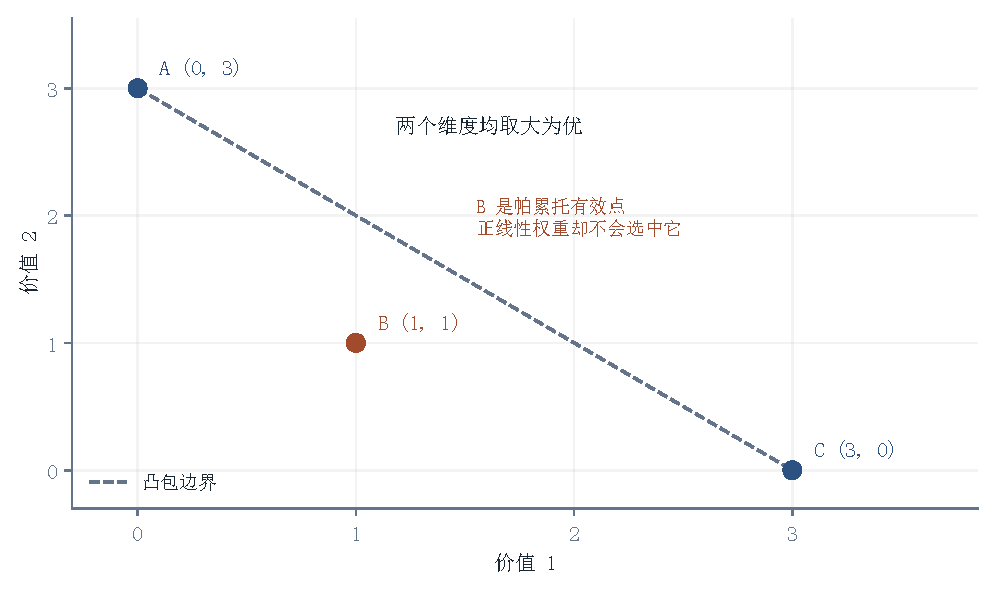
\includegraphics[width=\textwidth]{figures/unsupported-pareto.pdf}
\caption{可行集只有$A=(0,3)$、$B=(1,1)$与$C=(3,0)$，两个维度均取大为优。$B$不被其他点支配；但对$0\leq w\leq1$，$\max\{3w,3(1-w)\}\geq1.5>1$，线性加权不会选择$B$。}
\label{fig:mechanism-unsupported-pareto}
\end{figure}


\subhead{为什么这些位置长期报酬偏低}

如果这些位置承担着关键功能，一个自然的问题是它们为什么在很长一段时间里报酬不高。这个问题有两个答案，都是结构性的。第一是它们的价值难以度量。照护的成果是“没有出事”，教育的成果是“二十年后这个人过得如何”，事故调查的成果是“没有发生的灾难”。这些结果没有可比的计数，因此在以可量化指标为分配依据的体系里，它们的位置被系统性地压低。这是一个度量问题，不是价值问题。

第二是报酬形成的制度条件。某些经验与关系需要持续积累，供给扩张较慢；实际支付还取决于家庭资源、公共预算、雇佣规则与议价能力。私人服务可以扩大部分供给，也可能扩大获得服务的差距。功能的重要性、相对稀缺性与劳动者所得，必须分别观察。

\subhead{这个判断的边界}

验证、照护和长期塑造的相对稀缺性，需要与现有技术水平和制度配置共同判断。有些流程成本高，是因为缺少改造；另一些环节则承担了确有必要的功能。保留什么，取决于该功能如何被证明、能否用更低成本实现，以及取消后由谁承担损失。

这些功能也有身体消耗、责任压力、情绪劳动与机会成本。进入所需的长期投入，可能把缺乏时间和资源的人挡在外面。培养支持、公共支付、合理工作条件与进入机会，需要和技术工具一起改善，重要性才有机会转化为稳定供给与公平报酬。

如果价值最终沉淀在这些位置上，那么决定哪些问题值得投入的问题就变得更加关键。机器可以在给定的目标下高效搜索，但目标本身从哪里来，是接下来必须回答的问题。

\section{第三原则：共生原则}

沉淀区给出了位置，不完备性给出了理由，剩下的问题是这些位置与人之间是什么关系。共生容易被读成一种温和的道德表述，仿佛两种东西互相需要，于是应该彼此友好。这里的用法要窄一些，它描述的是一种能量形式上的互补：一方是可以在给定地形上高速移动的能力，另一方是必须靠时间积累才能形成的位置。第三原则处理的就是这种互补的分工，以及分工之后哪些阻力必须被保留。

\subsection{分工的本质：动能与势能}

动能取决于运动状态，势能取决于相互作用系统的位形。在近地面条件下，把1千克物体缓慢抬高1米，重力势能约增加9.8焦耳；完成得更快，需要在更短时间内提供相应功率。这里借用运动与位置的区别，考察可快速调用的能力与依赖长期关系形成的资格。后者的形成条件，需要从经验、承诺与制度中说明。

\subhead{可以瞬时供给的一侧}

信息处理也要支付物理代价。室温下擦除一个比特的兰道尔下限约为$3\times10^{-21}$焦耳，\cite{landauer1961} 与抬升重物所需的能量可以采用同一单位比较。差别在于操作对象、实际能耗和系统边界。复制模型、部署实例和执行动作分别需要计算、传输、存储与执行资源，某一环节变便宜，并不直接给出整条任务链的成本。

把这两个数字放回同一个比值里，量级差别就可以写成，

\begin{equation}
\frac{E_{\text{抬升}}}{E_{\text{擦除}}}=\frac{mgh}{k_{\mathrm{B}}T\ln 2}\approx 3\times10^{21}
\end{equation}

式中，$E_{\text{抬升}}=mgh$ 为把质量为 $m$ 的物体抬升高度 $h$ 所需的机械功，单位为焦；$m$ 为质量，单位为千克；$g$ 为重力加速度，单位为米每二次方秒；$h$ 为高度，单位为米；$E_{\text{擦除}}=k_{\mathrm{B}}T\ln 2$ 为擦除一个比特在热力学上允许的最小耗散，即兰道尔极限，单位为焦；$k_{\mathrm{B}}$ 为玻尔兹曼常数，单位为焦每开；$T$ 为环境温度，单位为开；$\ln 2$ 为 2 的自然对数。取正文所用的 1 千克、1 米与室温，右侧的数值约为 $3\times10^{21}$，也就是说，抬升一次重物所耗的能量相当于这个量级的比特擦除次数。这个式子的含义是：信息操作与物质做功不在同一个量级上，用算力总量去推断能改变多少物质，在物理上从一开始就不成立。适用条件需要一并给出：比值随质量、高度与环境温度变化，正文的 $3\times10^{21}$ 只对应它给定的那组取值；兰道尔极限是可逆擦除的理论下界，实际器件的能耗远高于它，因此这个比值给出的是量级判断，不是工程核算。

计算一侧的实际开销可以测量。Patterson等估计，训练GPT-3的电力消耗约为1287兆瓦时，相应碳排放估计约为552吨二氧化碳当量。\cite{patterson2021carbon} 这是特定训练任务与核算口径下的结果。训练、推理、实例部署和长期维护分别占用资源，能力的复制始终依赖供电、硬件与运行安排。

\subhead{必须积累的一侧}

再看必须积累的那一侧。人的位置大多不是由速度构成的，而是由一系列不可跳过的过程累积而成：技能的形成依赖重复到身体结构发生改变，判断力的校准依赖真实后果的反复反馈，信任的建立依赖多次守约，关系的内容依赖共同经历过的时间。这些过程的速率由生理和社会过程决定，不因为外部信息处理变快而变快。它们更接近势能：积累缓慢，一旦形成可以持续释放，而且不能在个体之间自由转移。这笔账也解释了为什么人无法通过“更快地学习”来追平前一节所述的那种速度优势：即使学习效率提高，能力形成的物理过程仍然需要时间，而这段时间本身就是势能的一部分。谁支付了这段时间，谁就获得了这段位置。

这类积累的速率不是估计值，行业标准把它写成了明文门槛。美国联邦航空管理局要求民航机长在取得执照前至少积累 1500 小时飞行时间，这条规则在 2009 年科尔根航空事故之后被写进法规，理由是低飞行时数的机组在突发情形下的处置能力不足。\cite{faa2013atp} 医疗行业的结构类似：一名外科医生从医学院毕业到独立主刀，通常需要五到七年的住院医师训练，专科方向还要更长。这些年限不能被购买，也不能被转让：执照可以考取，飞行小时数只能积累；资质可以被认证，手术的手感只能由自己的病例形成。势能的定价困难正来自这里，它没有替代品，因此无法通过增加供给来降价。

把两侧合起来，分工的内容就清楚了：一侧负责在给定地形上高速搜索，另一侧负责提供地形并承担地形错误带来的后果。这不是能力上的分工，因为定义地形并不需要更强的算力；它是位置上的分工，因为势能只能由承担了积累代价的一方持有。这一点和前一节的结论接得上：目标不能由系统内部生成，而外部的判据只能由那些已经支付了代价、并且会被自己判断错误所改变的位置提供。

\subhead{两种时间尺度的剪切应力}

两种时间尺度并置在一起，必然产生剪切应力。绘图的一侧以年为单位工作，登山的一侧以天甚至小时为单位工作，两者之间的速度差不会被技术消除，只会随着工具变快而扩大。它的表现形式都很具体：标准更新慢于能力变化，制度调整慢于市场节奏，个人的长期计划跟不上工具的换代周期，而在这些错位里，处在慢一侧的人会持续感到被拉扯。把这种张力说成需要消除的病灶是一种误读，因为消除它只有两条路，让慢的一侧加速或者让快的一侧停下：前者受内禀速率约束无法实现，后者要求放弃能力上的收益。可行的做法是承载张力的结构，把一部分判断留在慢的一侧，同时让快的一侧在明确的边界内运行。

\subhead{这条界线的限度}

这个分工必须接受几处限定，否则它会被读成一种身份宣告。动能与势能可以互相转化，所以这条界线不是天赋的界线：机器同样可以积累位置性资产，一座数据中心、一套被反复验证的流程、一个被市场接受的品牌，都具有势能的性质；人同样参与搜索，日常判断里大量成分是快速的模式匹配。真正的分界不在物种，而在代价能否转移：如果代价可以被转移、被保险、被外包、被回滚，那么位置就没有被真正承担，势能也就不成立。反向的限定同样成立：占据了一个位置不等于判断正确，势能提供的是资格而不是正确性。历史上由处在承受位置的人做出的灾难性判断并不少见，这个事实不能靠分工来抹掉。分工能够支持的只是一条程序上的要求：给出地形的人必须在这片地形上行走，并且能够被后果改变。

机器一侧的积累同样可以量化。一座先进制程晶圆厂的投资在百亿美元量级，建设周期以年计，投产后还要经过良率爬坡才能形成可以交付的产能；这套资产的重量体现在它不能快速迁移，也不能在需求变动时被随意改产。\cite{verheyde2019tsmc} 这些约束与算法进步无关，它们由建筑、设备、材料供应和工程人员的实际速度决定。位置性资产因此不是人类专属，它也不随模型迭代而瞬时重置：把一套能力复制到新的实例上只需要分钟，把一条产线建起来仍然需要数年。

\subsection{人作为绘图师：地形从哪里来}

问题已经落到目标本身从哪里来。要看清这个问题，最好从优化问题的写法入手。一个优化问题写作

\begin{equation}
x^{*} = \arg\max_{x \in \mathcal{X}} f(x)
\end{equation}

求解这个问题的意思是：在允许的集合 $\mathcal{X}$ 里，找出使目标函数 $f$ 取值最大的那个 $x$。算法工程的大部分工作是在这一层之下完成的：设计更好的搜索策略、更快的近似、更有效的表示，让 $x^{*}$ 被更快更准地找到。这个式子里有一项从来不参与求解，它只是被使用，那就是 $f$。目标函数不是优化过程产生的结果，而是优化过程的输入。一个算法能把 $f$ 最大化到小数点后多少位，是一个能力问题；$f$ 应该是什么，不属于这个问题的范围。

这个区分看起来是技术性的，但它决定了后面所有讨论的边界。当人们在讨论通用智能何时到来时，讨论的是求解能力那一侧；当人们在讨论这项技术会带来什么后果时，讨论的往往是 $f$ 那一侧，而那一侧并没有跟着一起进步。适应度景观是同一个结构在生物学中的表述：一个物种在景观上攀爬，向更高的适应度移动，但景观的形状由环境给出，不由攀爬者给出。\cite{kauffman1993} 机器优化路径，人定义地形。这个分工不是能力上的分工，因为定义地形并不需要比优化路径更强的算力，它需要的是另一种东西。

\subhead{地形从哪里来}

那么地形是什么，它从哪里来。地形不是一条可以直接读出的东西，它是一个社会在漫长时间里通过大量具体判断累积形成的。什么算进步，什么风险可接受，什么未来值得追求，什么代价不能转嫁，这些问题的答案从来没有被完整地写下来过，它们分布在法律、习俗、专业规范、公共舆论和一代人的共同经历里。这类答案有几个特征，使它们不能被自动化。

第一个特征是它们包含不可通约的比较。一项减少碳排放的技术和一项提高粮食产量的技术，哪一个更重要，这个问题没有一个共同单位可以度量。成本收益分析可以给出一个数字，但那个数字来自对两类价值的相对权重的预先设定，而权重本身就是争议所在，把它写成一个标量函数，只是把争议隐藏在了参数里。第二个特征是它们依赖代价的分布。同一个总收益，如果代价集中在少数无法议价的人身上，它和一个总收益略低但代价分散的方案的比较结果，取决于社会对公平的判断，这个判断不能由总效用来代替。这也是为什么基础设施选址、环境许可、药物审批这类问题无法被纯技术化处理：技术可以计算总量，不能决定分布。

第三个特征是它们随时间变化。三十年前被普遍接受的代价转嫁在今天不可接受，反过来也一样。地形的这一部分性质意味着目标函数不是一次给定就固定的，它需要在新的信息和新的承受经验中不断修订。这三个特征指向同一个结论：地形是社会在自己承受后果的过程中逐步给出的，它不是被发现的知识，而是被做出的决定，因此它带有决定的一切特征：有争议、会改变、需要有主体来承担。

\subhead{四类只能由承受者回答的问题}

把上面的一般论述落到具体，有四类问题在结构上必须由承受后果的主体来回答，而它们各自不能被技术评估替代的原因略有不同。什么算进步，这个问题的答案决定了资源的长期流向。以产出总量衡量进步和以人的能力发展衡量进步，会导向完全不同的技术路线。这个问题不能被交给一个只优化已有指标的机构，因为指标的设定本身就是这个问题的答案，把指标设定权交出去等于把问题本身交出去。

什么风险可以接受，这一类的困难在于阈值。每一项技术在带来收益的同时带来风险，风险的可接受程度取决于一个社会愿意让谁承担多少代价。核电站的选址、基因编辑的边界、自动驾驶的接管策略、新药的审批速度，这些问题都需要一个有权做出决定并且承担决定后果的主体；技术评估可以提供概率分布，不能提供接受阈值，因为从概率到一个“可以接受”的判断之间，跨过的是一段价值论证，不是一段计算。什么未来值得追求，这一类的困难在于时间尺度。载人航天、深空探测、基础科学、生态修复，这些方向在几十年尺度上都无法用投入产出比来辩护。选择一个长周期方向，本质上是让当代人为后代人的可能性支付成本，而这个选择必须由能够代表未来的人做出。

什么代价不能转嫁，是前面三个的底线形式。当一项技术把成本转移给没有参与决定的一方（转移给未来、转移给生态、转移给缺乏议价能力的群体），这个转嫁在技术上可能是最优的，在结构上是不可接受的。设定这条底线不需要技术知识，需要的是承认承受者有权拒绝，而“有权拒绝”这件事本身无法从任何优化过程里推导出来，它必须被作为一个前提写进去。

\subhead{这不是能力优先的立场}

决定目标涉及受影响者的资格。关于“由谁承受什么”的决定，需要让承担风险的一方参与，或由具有相应授权的机构代表。机器可以提供候选、预测和论证，参与者也需要借助专业知识；决定的合法性还须满足程序、权利与救济的要求。承担后果是一项重要条件，不能单独替代授权。

用这个标准看，绘图师的资格不来自计算能力、不来自知识总量、也不来自自我意识。它来自一个更朴素的事实：给出地形的人必须在这片地形上行走，他的判断会以他自己的代价被检验。一个系统如果在判断出错时不承担任何后果，它的判断就缺少校准来源，无论它的推理能力有多强。把 AI 放进目标设定的位置会有一个特殊困难。不是因为它算得不够好，而是因为它的输出和目标设定的正确性之间没有反馈回路。人类设定者判断错了，会在若干年后看到后果并以某种形式付出代价；一个没有承受边界的系统在这条链上是断开的，错误不会被回流，因而不会被修正。

需要补一句限定，否则这个立场会变得过强。承受位置给出的是资格，不是正确性。有人承受后果并且做出的判断仍然是错的，这是常态，历史上由承受者做出的灾难性判断数不胜数。这个论证能支持的只是程序上的要求：目标设定权应当归于承担后果的一方，并且这一方必须有能力被后果改变。它不支持任何关于判断质量的保证。

\subhead{绘图是个持续动作}

还有一个容易被误解的地方：绘图不是一次性给出一个目标，然后交给机器去执行。地形在真实过程中持续变化。技术改变了可行的选项集合，选项集合的改变又改变了价值排序，价值排序的改变使原本不可接受的代价变得可以接受，或者反过来。这个过程没有终点，也不会收敛到一个稳定的目标函数。扮演绘图师的角色，意味着持续参与这个过程，而不是在某一天宣布目标已经确定。

这件事在实践中表现为一系列不那么宏大的动作：参与标准制定，参与事故调查，参与伦理审查，参与资源分配的讨论，在技术评估中坚持把分布问题摆上桌面，在长期项目上保留说不的权力。这些动作大多缓慢、不产生可见成果，也无法通过更好的算法来加速。它们的作用不在于给出更好的答案，而在于保证答案始终有人负责。代价是清楚的：这意味着人不能把判断的责任交出去。当一项技术被证明比人做得更好时，把决定权交给它的诱惑是真实的，而且在很多局部问题上交出决定权确实是正确的做法。要区分的是这两类问题：在给定目标下的求解可以交出去，目标本身不行。这条线不是由技术能力划定的，它由承受结构划定。

承认绘图是持续动作之后，另一个更实际的问题立刻出现。既然阻力并不都值得保留，也不都应当删除，那么在具体的场景里，哪些阻力承担着筛选、校准或约束的功能，哪些只是历史留下的损耗。这个问题不能靠态度回答，它需要一个可以逐项执行的判据。

\subsection{必要摩擦：哪些阻力应当保留}

\subhead{为什么必须区分}

前面关于高黏滞位置承载价值的论证容易引出一个错误的结论：如果高黏滞位置承载价值，那么保留阻力就是好事。这个结论既不正确也没法操作，因为阻力从来不是一个整体，它是一堆性质完全不同的东西的集合。同一项技术可以在一次改动中同时消除三类完全不同的摩擦，而它们的后果差别极大。

设想一家医院把纸质病历换成电子系统。录入时间缩短了，这是效率改进；重复检查减少了，这是资源浪费的消除；但同时，医生在病历上写下的第一手判断被结构化字段替代，那些无法被选项覆盖的观察失去了记录位置，而事后复核时，审阅者看到的是符合规范的表单，不再是医生的原始思考。第三种变化和第二种在表面上都是“减少了工作量”，在结构上完全不同。如果把这三类变化都归为摩擦的减少，就会得出一个笼统的判断，既不能指导技术设计，也不能指导制度安排。所以需要一个分类，而这个分类要能落在一处一处具体的阻力上，而不是停在态度层面。

\subhead{三类摩擦}

第一类是无效摩擦。它由组织惯性、信息不对称、流程冗余、工具落后、沟通损耗产生，不承担任何检验功能。医院里同一份信息在五个系统里各录一遍，行政审批要跑三趟窗口，公司内部因为部门壁垒重复开发同一套工具，都属于这一类。这类摩擦没有存在的理由，消除它不产生任何结构性损失，只产生收益。需要注意的是，无效摩擦对身处其中的人往往并不显得无效：它有历史原因，有人靠它获得位置，也有真实的风险规避动机曾经支撑它，因此识别它需要追问它在今天还挡着什么，而不是它当初为什么被建起来。

第二类是工程摩擦。它由物理约束和技术成本产生，是真实存在的但可以被压缩或转移。混凝土需要养护时间，芯片制造需要洁净环境和多层光刻，跨洋运输需要燃料和时间。这类摩擦不能被消除，但可以通过更好的工艺、更优的调度、更合理的资源投入来降低。压缩它的代价通常以资源或时间的形式在其他地方出现：压缩养护时间要加早强剂或者改变配比，压缩物流时间要空运或者提高库存。工程摩擦的处理原则因此是显式的，比较压缩成本与收益，选择总代价更低的方案，这个比较可以算，也可以被审计。

第三类是必要摩擦。它由系统需要承担的功能产生，消除它会造成功能缺失，而这种缺失往往不会立刻显现。验证、承责、身体接触、长期关系、公共讨论、风险暴露、教育中的慢形成，都属于这一类。它们的共同特征是：表面上看起来像是效率损失，实际上承担着筛选、校准或约束的作用，一旦被移除，系统会在某个延迟之后失去某项能力。三类之中只有这一类无法在当期被量化，而这恰恰是它在管理决策中最容易被牺牲的原因。\key{成熟技术的标志不是消除一切阻力，而是有能力区分无效摩擦与必要摩擦。} 这个区分不是价值立场，它要求对每一处摩擦追问一个具体问题：它现在在筛掉什么，或者阻止什么。
\begin{figure}[ht]
\centering
% >>>>>>>>>> figs/fig-friction-classes.tex >>>>>>>>>>
% 图 6-1  三类摩擦：同一项改动会同时动到三种性质不同的阻力
% 三行的差别不在"多"与"少"，而在移除之后会发生什么。
% 左侧色块给出类别与后果显现的时延；右侧三栏依次是来源、处置与移除的后果。
% 判定的三个问题写在正文里，本图只承担分类本身：
%   问一 移除后系统会不会在别处重建等效机制；
%   问二 代价由谁承担、收益由谁获得；
%   问三 把它压缩到极限会发生什么。
\begin{tikzpicture}[x=1cm, y=1cm, font=\small,
  rw/.style={rounded corners=1.5pt, line width=0.6pt},
  ct/.style={font=\scriptsize, text=ink, align=center, anchor=center},
  hd/.style={font=\scriptsize\heiti, text=slate, anchor=south}
]
\useasboundingbox (-0.30,0.80) rectangle (13.25,-6.42);

\def\cl{0.15} \def\cA{2.55} \def\cB{7.05} \def\cC{10.55} \def\cD{12.95}
\def\mAX{1.35} \def\mBX{4.80} \def\mCX{8.80} \def\mDX{11.75}

% ---------- 表头 ----------
\node[hd] at (\mAX,0.36) {类别};
\node[hd] at (\mBX,0.36) {来源};
\node[hd] at (\mCX,0.36) {处置};
\node[hd] at (\mDX,0.36) {移除的后果};

% ---------- 第一行：无效摩擦 ----------
\fill[rust!13] (\cl,0.00) rectangle (\cD,-1.75);
\fill[rust!30] (\cl,0.00) rectangle (\cA,-1.75);
\draw[rw, rust!55] (\cl,0.00) rectangle (\cD,-1.75);
\draw[slate!30, line width=0.4pt] (\cA,0.00) -- (\cA,-1.75);
\draw[slate!30, line width=0.4pt] (\cB,0.00) -- (\cB,-1.75);
\draw[slate!30, line width=0.4pt] (\cC,0.00) -- (\cC,-1.75);
\node[font=\small\heiti, text=rust!85, anchor=center] at (\mAX,-0.70) {无效摩擦};
\node[font=\scriptsize, text=slate, anchor=center] at (\mAX,-1.22) {后果时延：当期};
\node[ct] at (\mBX,-0.875) {组织惯性、信息不对称、\\流程冗余、工具落后};
\node[ct] at (\mCX,-0.875) {直接删除};
\node[ct] at (\mDX,-0.875) {无结构性损失};

% ---------- 第二行：工程摩擦 ----------
\fill[terra!13] (\cl,-1.95) rectangle (\cD,-3.70);
\fill[terra!30] (\cl,-1.95) rectangle (\cA,-3.70);
\draw[rw, terra!60] (\cl,-1.95) rectangle (\cD,-3.70);
\draw[slate!30, line width=0.4pt] (\cA,-1.95) -- (\cA,-3.70);
\draw[slate!30, line width=0.4pt] (\cB,-1.95) -- (\cB,-3.70);
\draw[slate!30, line width=0.4pt] (\cC,-1.95) -- (\cC,-3.70);
\node[font=\small\heiti, text=terra!90, anchor=center] at (\mAX,-2.65) {工程摩擦};
\node[font=\scriptsize, text=slate, anchor=center] at (\mAX,-3.17) {后果时延：数月};
\node[ct] at (\mBX,-2.825) {物理约束与技术成本\\（养护、光刻、运输）};
\node[ct] at (\mCX,-2.825) {比较压缩成本与收益\\之后压缩};
\node[ct] at (\mDX,-2.825) {代价以资源或\\时间形式转移};

% ---------- 第三行：必要摩擦 ----------
\fill[forest!13] (\cl,-3.90) rectangle (\cD,-5.65);
\fill[forest!30] (\cl,-3.90) rectangle (\cA,-5.65);
\draw[rw, forest!60] (\cl,-3.90) rectangle (\cD,-5.65);
\draw[slate!30, line width=0.4pt] (\cA,-3.90) -- (\cA,-5.65);
\draw[slate!30, line width=0.4pt] (\cB,-3.90) -- (\cB,-5.65);
\draw[slate!30, line width=0.4pt] (\cC,-3.90) -- (\cC,-5.65);
\node[font=\small\heiti, text=forest!85, anchor=center] at (\mAX,-4.60) {必要摩擦};
\node[font=\scriptsize, text=slate, anchor=center] at (\mAX,-5.12) {时延：跨管理周期};
\node[ct] at (\mBX,-4.775) {系统必须承担的功能\\（验证、承责、公共讨论）};
\node[ct] at (\mCX,-4.775) {保留；删除须先给出\\替代机制};
\node[ct] at (\mDX,-4.775) {功能缺失，\\延迟显现};

% ---------- 底部：两类误判的不对称 ----------
\node[font=\scriptsize, text=ink, anchor=north west, align=left]
      at ({\cl},{-6.02})
      {两个方向的误判不对称：保留无效摩擦是慢性损耗，删除必要摩擦是结构损伤。};
\end{tikzpicture}

% <<<<<<<<<< figs/fig-friction-classes.tex <<<<<<<<<<

\caption{三类摩擦。分类的依据不是量的多少，而是移除之后会发生什么；右端一栏给出三种后果，它们显现的时延自上而下依次拉长。这解释了为什么必要摩擦在当期管理决策中最容易被牺牲：它的代价要跨过管理周期才浮现，而收益的账面在当期。}
\label{fig:friction-classes}
\end{figure}

\subhead{判定的三个问题}

这个追问可以拆成三个可以逐项回答的问题。第一个问题是：如果移除它，系统会不会在别处重建一个等效机制。如果会，它属于无效摩擦或工程摩擦，因为系统并不真正依赖它。航空业的行李安检曾经由人工开箱完成，后来改成 X 光机加抽查，效率提高了几倍，安全水平没有下降，因为检查的功能被更高效的手段承担了。相反，学术界的同行评议如果被移除，替代机制必须提供同样的东西：让工作在发表前经过有资格的反对者检验。目前没有更便宜的替代方案，所以它尽管慢、尽管有偏见，仍然属于必要摩擦。

第二个问题是：它的代价由谁承担，收益由谁获得。这一类摩擦如果承担者和受益者不是同一方，通常意味着它是被转嫁的成本，而不是被设计的功能。平台把内容审核的成本转移给创作者和用户，用户的注意力成本被转移给广告主，这类结构中的“低摩擦”往往只是把摩擦挪到了看不见的地方。反过来，如果承担者和受益者是同一方，而且代价换来了真实的信息或能力，它更可能是必要的。这个问题的价值在于它能把讨论从“效率高低”转到“代价落在谁身上”，而后者才是真正需要被裁决的部分。

第三个问题是：把它压缩到极限会发生什么。工程摩擦在这个测试下表现良好，压缩到极限无非是成本上升，不会改变系统的性质。必要摩擦在这个测试下会失效：验证压缩到零，系统就不再知道什么是真的；教育中的慢形成压缩到零，得到的是通过考试的人，不是具备能力的人；公共讨论压缩到零，得到的是快速共识，不是被检验过的共识。这个问题之所以好用，是因为它不需要知道摩擦的成因，只需要设想一个极限情形。三个问题不能完全机械化，但比“阻力越大越好”或者“越快越好”都要可操作。

\subhead{与反技术立场的分歧}

把必要摩擦单列出来，容易被读成一种反技术的姿态，因此需要把分歧说清楚。Theodore Kaczynski 在 1995 年提出过一个论证：工业技术系统会持续扩张，逐步剥夺个人自主，因此应当被瓦解。\cite{kaczynski1995industrial} 他的论证中有一部分值得认真对待：技术系统确实会重新组织人的生活，而且这种重组往往不经过个人同意。但他的结论把技术当作一个整体来处理，因此只能得出全盘接受或全盘拒绝两个选项，而这两个选项在实践中都不可用。

必要摩擦的分析给出的是一条不同的路径。它不追问技术应不应该存在，而追问每一处具体的阻力承担了什么功能。这个问法允许同时做出两个方向相反的判断：一套审批流程应当被彻底删掉，而同一天上线的另一项自动化应当被紧急叫停。它不承认“技术本身”这个主语，只承认具体的机制在具体的位置上做了什么事。这个立场的代价是它不提供简洁的口号。它不能给出一个总的方向，只能给出一个逐项判断的程序，而逐项判断需要领域知识、需要理解系统的实际功能、需要在信息不完整的情况下做出取舍。这使它在公共讨论中处于劣势：反对技术的人有清晰的态度，支持技术的人有清晰的收益，管理摩擦的人只有一份长长的、需要专业判断的清单。

\subhead{两种误分类}

实践中最常见的错误不是分不清三类摩擦，而是在两个方向上系统性地误判，而这两个方向的错误并不对称。第一个方向是把必要摩擦当成无效摩擦删掉。这类错误几乎总是以效率为名，而且短期效果良好。企业取消资深员工的复核环节以提高交付速度，头几个月指标上升，一年后事故率上升，而事故的成因很难追溯到那次流程简化。教育压缩实践环节以增加课时覆盖，学生的考试成绩可能提高，动手能力在毕业后才暴露问题。这类错误的共同结构是：功能被移除，损失延迟出现，因果链在时间上被拉长到超出管理周期。

第二个方向是把无效摩擦当成必要摩擦保留。这类错误的辩护词通常是“传统”“经验”“风险”，它在稳定的组织里特别常见，因为保留摩擦对在位者有利。这类错误的成本是持续的、可见的、容易被抱怨的，所以相对容易被纠正，只要有足够的外力推动。两个方向的错误因此不对称：保留无效摩擦是慢性损耗，删除必要摩擦是结构损伤。这个不对称意味着，在信息不足的情况下默认选择应当是谨慎的，但这不等于把所有阻力都保留。谨慎的正确含义是：对每一处待删除的摩擦，要求提出者说明它在筛掉什么；如果提不出，就删掉；如果提得出，就要求给出替代机制。

到这里，一个自然的问题出现了。既然摩擦需要被逐项区分，而区分的判据又要求承担者与受益者对齐，那么谁来完成这件事。个体面对的是一个持续把人推向最短路径的环境，组织面对的是当期指标与长期能力之间的取舍。这两层都不是分类问题，而是实践问题。

\section{第四原则：递归优化原则}

前面三条原则处理边界、标准与分工。本节继续检查维持它们的更新过程：实践带来证据，证据推动标准修订，修订又改变下一轮行动。回路可以形成稳定状态，也可以随环境持续变化，具体行为取决于更新规则、延迟与外部输入。

把这个回路写成迭代的形式，它的行为由收敛条件决定，

\begin{equation}
x_{n+1}=g(x_{n}),\qquad \left|g'(x^{*})\right|<1\ \text{时迭代收敛到不动点}\ x^{*}
\end{equation}

这里先以一个标量参数$x_n$说明评价更新，$g$为连续可微的更新映射，$x^*$为不动点。$|g'(x^*)|<1$给出局部渐近收敛的充分条件；导数绝对值大于1时，不动点不稳定，等于1时还须进一步分析。多参数更新则要考察雅可比矩阵的特征值。价值与环境随实践改变，可能形成新的稳定状态，也可能持续变动，具体行为由更新规则和外部扰动决定。

\subsection{反向算法：主动引入摩擦}

\subhead{问题的位置}

前面的讨论给出的是价值流向和人的重新定位，这些是结构层面的判断。结构层面的判断有一个弱点：它正确，但不能直接指导一个人在星期一早上做什么。压力落在个体身上时，不会以结构分析的形式出现，而是以一连串具体选择的形式出现：用不用导航，写不写这段文字，回不回这条消息。这一节处理的就是这些选择，但处理方式不是给出一份清单。

先说清楚这一节不做什么。它不主张拒绝技术，也不主张人为制造困难。一个人的日常决定散布在无数细小的场景里，任何一份统一的清单都会在第一次遇到例外时失效。这里要处理的是一个更窄的问题：低黏滞系统会持续把人的行为推向某些固定方向，如果一个人想在这些方向上保留一部分自主，需要满足什么条件。这不是关于意志的问题，而是关于边界维护的问题，因此它可以用结构的方式来说。

\subhead{系统把人推向哪里}

要保留自主，先要看清推力指向哪里，因为反抗一个方向的前提是知道方向。低黏滞系统对人行为的塑造可以归纳为四个方向，而它们各自都是被优化出来的，不是被设计出来的。第一个方向是最短路径。只要存在一条更短的路径，系统就会把它找出来并设为默认，用户每一次手动绕开都在付出额外成本。第二个方向是即时反馈。反馈延迟越长，用户越容易流失，因此所有环节都在被压缩，包括那些本来需要时间的环节。

第三个方向是偏好闭环。系统从一个人的历史行为中推断他的偏好，然后按这个偏好供给内容，供给的结果又成为新的历史行为，闭环因此逐步收窄。这个过程不需要任何恶意，它只是让预测更准的必然结果，而更准的预测意味着更少的意外。第四个方向是无痛满足。凡是能提供的满足，系统都倾向于以最低成本提供，因为低成本意味着更高的使用频率，而高成本的部分被逐步剥离。四个方向的共同点是它们都提高短期指标，因此不需要任何人推动，它们自己就会发生。

这些推力不是外来的胁迫，它们不禁止任何事。一个人随时可以关掉推荐、可以选择手动路线、可以拒绝生成。问题在于每拒绝一次都要付出成本，而这些成本是持续的、累加的、没有外部奖励的。在一个推力持续存在而阻力没有回报的环境里，行为的分布会向推力方向偏移，这不是判断力的问题，是概率的问题，除非有某种机制能稳定地抵消它。

\subhead{保留非最优接口}

能稳定抵消它的机制，是把一部分非最优的选择固定下来，使它不再需要每次重新决定。这就是所谓保留非最优接口的意思。接口在这里指的是人与世界接触的那一层：怎么走一段路，怎么读一本书，怎么完成一件东西，怎么和一个人维持联系。把某些接口刻意保留在非最优状态，代价是明确的效率损失，收益是这些接口所承载的能力不会退化。

具体的形式因场景而异，但有几类被反复验证过。第一类是等待。主动接受某些延迟，不用缓冲把它填满，让间隙重新成为一个可以思考和退出的位置。第二类是身体训练。它是最不容易被代劳的接口，因为肌肉、心肺和协调性的改变必须由本人的重复动作产生，而且这个过程无法被加速，训练量的积累和能力的提高之间有硬性关系。第三类是线下关系。面对面接触携带的信息量和约束强度高于远程交流，而它的成本也更高，因此是第一批被替代的接口。

还有几类性质稍有不同的。手作与制作把人和材料直接接上，材料会抵抗，会出错，会留下不可撤销的痕迹，这些性质在数字工具里被全部移除。难读的文本要求持续的注意力，不能跳读，不能摘要，读者必须自己完成理解过程。长期项目在几个月到几年的尺度上没有任何阶段性成就，它的回报集中在完成时刻，因此和即时反馈系统正好相反。无即时反馈的承诺要求一个人在没有回报的期间继续兑现。偶遇与随机性把非最优的结果保留下来，使偏好闭环无法完全闭合。

这些活动的价值在于它们仍能形成所需要的能力。若直接练习比完全代办更能维护判断，就可以把练习安排成稳定的默认；若工具提供更好的反馈，也应采用。相对即时产出的效率损失，需要与长期能力收益一起比较。

\subhead{为什么不是意志力问题}

把上面的做法理解为自律，会引出两个错误的推论。第一个是把它当成道德要求：能坚持的人更有品格，坚持不了的人是自己不行。第二个是把它当成个人偏好：愿意怎样生活是各人的选择，不需要理由。两个推论都错在同一个地方，它们把这件事放在个人层面处理，而它的问题出在环境的反馈结构上。

低黏滞环境不是一个人可以选择退出的外部条件，它已经嵌入了工作、社交、支付、出行和求医的每一个环节。在这种条件下，要求一个人靠意志力持续逆着环境走，等于要求他一生都在消耗同样的资源，而且这个消耗不会带来任何外部承认。这个要求是不现实的，不是因为它太难，而是因为它没有稳定的支撑结构。真正有效的做法不是在意志层面加码，而是在结构层面减少需要意志介入的次数：把某些接口从选项中移除，让它们不进入每次决策的比较。

这个区分的实践含义是具体的。一个把手机放在另一个房间的人，并不是在考验自己的意志，他是在改变自己需要做出的决定数量。一套固定的作息安排之所以比每天决定几点睡更有效，也是因为它把决定变成默认。这些做法在表面上像是自律技巧，实质上是把一部分选择权从当下的自己手里拿走，交给一个事先设定好的安排，从而抵抗环境对行为分布的持续拉扯。

\subhead{代价的方向}

需要把这一节的限度说清楚，否则它会变成一份生活方式建议，而生活方式建议在结构上站不住。这些做法的代价是真实且不对称的。保留非最优接口的人会在具体的场合输给采用最优路径的人：更慢，更累，产出更少，而且在大多数评价体系里得不到任何补偿。这个代价是持续的，而收益是长期的、分散的、难以指认的，因此在个人层面很难形成稳定的正反馈。

这意味着这一节的建议不构成一种普遍可行的方案。对能够承担这个代价的人，它是有效的；对时间、精力或经济条件不允许的人，它是奢侈的，把它普遍化会变成对处境不利者的又一次指责。能承担的范围内做多少，取决于具体情况，而更重要的是认识到一件事：个体层面的调整只能减缓偏移的速度，不能改变偏移的方向。方向由评价函数决定，而评价函数的改变不是个体能完成的动作。把这一层说清楚，是为了避免把结构问题伪装成个人修养问题，也是为了指出下一步该往哪里走：从个体转到组织，从个人选择转到那些决定评价函数的地方。

\subsection{高黏滞组织：信任与验证的重建}

\subhead{从个体到组织}

把个体的调整做到限度之后，会遇到一个不由个人决定的东西：方向由评价函数决定，而评价函数不由个人设定。评价函数存在于组织中，因此改变它需要在组织层面完成。这一节处理的就是这类组织，但切入的角度不是管理，而是一个具体的功能问题：在一个生成成本趋近于零的环境里，什么样的组织还在生产别的东西。

要看清这个问题，可以先看一个反差。同样面对生成式工具，两类组织的反应完全不同。一类组织立刻把它接入生产流程，交付速度上升，人力需求下降，报表改善；另一类组织允许使用，但同时增加了验证环节、收紧了发布权限、延长了关键判断的复核周期，短期内效率反而下降。按通常的效率标准，第一类组织是赢家。但如果把时间尺度拉长，并且把事故率、召回率、返工率、诉讼成本和人员流失一起计入，两类的排序可能会反过来。这个反转会不会发生，取决于该组织的产出在多大程度上依赖判断的正确性，以及错误一旦发生的代价有多大。

\subhead{凭据生成器}

那些排序可能反转的组织，有一个共同的功能，可以称之为凭据生成。凭据在这里指的是一个可以被第三方依赖的判断：这份检测报告可信，这个药可以上市，这座桥能承重，这份审计意见可以拿去贷款，这个判决可以执行，这篇论文的结论可以被引用。凭据的价值不在于它有多新颖，而在于它背后的判断已经经过了某种检验，而且这个检验的过程可以被追溯和复核。

大学、实验室、医院、工程机构、法院、审计机构、认证机构、事故调查委员会，都属于凭据生成器。它们看起来效率低下：审稿要几个月，临床试验要几年，工程验收要停工期，判决要经过多级审理，事故调查要反复取证。这些延迟经常被批评为官僚主义，其中也确实有一部分是。但把延迟整体删除之后，这些机构就不再生产凭据，它们只生产意见，而意见不能作为凭据被依赖，因为它没有承载责任的构造。

理解这个功能之后，就能看清这些机构的慢在哪里是有意义的。有意义的慢集中在判断的形成环节：证据如何收集，反方意见如何进入，结论如何被复核，谁有权签署。无意义的慢集中在行政流转环节，这些环节的删除通常不损害凭据质量。可信组织的价值，不在于生成更快，而在于让判断有地方对账。对账的意思是：当一个判断被质疑时，有能力回到形成这个判断的过程，并检查每一步是否成立。

\subhead{四类慢变量}

凭据生成依赖于几类慢变量，它们各自对应一种不能压缩的过程。第一类是验证周期。一个结论要被确认为可靠，需要经过独立的重复，而重复需要时间。药物的三期临床、材料的长期老化测试、算法的对抗测试、结构的安全系数验证，都属于这一类。验证周期可以被组织得更好，但不能被跳过，因为跳过之后得到的不是更快的结论，而是一个未被验证的结论。

第二类是信任积累。一个机构的可信度由它过去的行为记录决定，而这个记录只能通过时间生成。一家医院需要多年的诊疗记录才能建立转诊信誉，一个认证机构需要经手足够多的案例才能被市场接受，一个实验室需要若干篇经得起复查的论文才能获得同行信任。信任的积累慢而摧毁快，这个不对称使它对机构的激励结构提出了很高的要求：任何一次为了短期收益而放松的验证，都可能把多年积累一次性抵消。

第三类是责任链的清晰度。判断由谁做出、依据什么、在什么权限范围内、出了错由谁承担，这些问题必须在判断形成之前就有答案，事后补是不行的。事故调查中最常见的问题不是找不到责任人，而是责任链在制度设计阶段就不存在，导致事后无法归属。第四类是慢变量本身的保护机制。承上所述，评价体系天然偏好可量化的短期指标，因此那些需要长期投入的环节会被持续挤压，除非有明确的机制保护它们：终身教职、独立预算、法定的复核程序、行业自律规范，这些安排的历史来源各不相同，但功能相同：让某些环节不必为当期的产出指标负责。

\subhead{为什么市场不会自动提供}

如果凭据生成这么重要，一个自然的问题是为什么市场不自动产生足够的供给。这个问题有几个层次的答案。第一层是时间错配。凭据的价值在被需要时才显现，而事故是低频事件，因此在两次事故之间的长周期里，投入凭据生成的组织看起来只是在浪费钱。没有经历过事故的决策者很难为它付账，而经历过事故的决策者往往已经不在位置上了。

第二层是收益的不可独占性。一个机构投入成本建立高标准的验证流程，它生产出的可信度有一部分会外溢给整个行业：客户会把整个行业的标准提高，而不只是信任这一家。这种正外部性使个体投入低于社会最优水平，这是认证、标准、审计这类活动长期需要公共或行业层面强制的原因。第三层是竞争压力下的向下竞次。当同一市场中有一方降低了验证标准并把节省的成本让给客户，其余各方在短期内有强烈的动机跟随，而后果的显现要等到下一次事故。这个结构在金融、航空、建筑、食品、医药领域都反复出现过，每一次的应对方式都是事后监管，而监管的时滞本身就是代价的一部分。

这些机制说明，凭据生成不能完全靠市场自发提供，但它也不能完全靠行政命令提供，因为凭据的可信度恰恰来自生成机构的独立性。这个张力没有一般解，只能在具体领域里通过制度安排来平衡，而平衡点在不同领域差别很大。

\subhead{组织内部的改变}

回到最初的问题：一个组织要维持凭据生成能力，需要在自己内部做什么。最容易想到也最容易被做错的，是设置验证环节。单纯增加一道审批不生产凭据，它只生产签字，因为审批者如果没有足够的信息和动机去实质检验，他的签字只是在分摊责任，不是在确认判断。有效的验证需要三个条件同时满足：验证者能看到原始材料而不是加工后的摘要，验证者的评价不受被验证方的直接控制，以及验证者做出否定判断时不会受到惩罚。

除了验证，还有两处需要调整。一是把慢变量的保护写进考核。如果所有指标都是季度产出，那么长期投入必然被牺牲，这不是执行问题，是指标结构问题，唯一的解法是让一部分评价周期长于任期。二是保留可以被追溯的记录。生成式工具让产出变得容易，也让产出的来源变得难以分辨，因此一份记录了谁在什么依据下做了什么判断的档案，其价值在上升。这类记录在平时被视作负担，在事故发生时是唯一能重建过程的东西。

需要承认这套安排的成本。一个维持凭据生成能力的组织，在生成速度上会持续落后于不维持的组织，而这个落后是可见的、可量化的、会在竞争中被反复计入的；它换来的东西是不可见的，因为它体现在没有发生的事故里。这个不对称是这类组织长期面临的困境，也是它们需要外部制度支持的原因。个体在这一层能做的有限，但组织层面的选择决定了评价函数，而评价函数决定了前面那些个体做法能不能长期维持。如果组织不保护慢变量，个体的保留非最优接口就只能在私人时间里进行，而私人时间也是被同一套评价函数压缩的。

到这里，个体和组织各自的动作都已经交代清楚，但它们都建立在一个尚未检查的假设上：人被当作产出能力来管理，因此保留位置的问题被理解成保留产出能力的问题。这个假设看起来很自然，实际上它有一个可以追溯的来历，而把这个来历看清楚，前面两节的做法才有可能被放在正确的位置上。

\subsection{负熵体验者：功能性与体验性的正交}

\subhead{一个没有被检验的前提}

如果人承担的是定义地形的角色，那么人自身应当被理解成什么，就成为一个必须重新回答的问题。把人当作产出工具的旧框架，在这个位置上已经不够用了；这个判断需要一个正面的替代，而在给出替代之前，先要看清楚被替代的是什么。关于人工智能与人的讨论，绝大多数都建立在一个没有明说的前提上：人的价值等于人的产出。这个前提如此普遍，以至于争论的双方都在用它。乐观的一方说机器会把人从重复劳动中解放出来，让人去做更有创造性的产出；忧虑的一方说机器会取代人的产出能力，使人失去位置。两种说法方向相反，前提相同。

如果这个前提是对的，那么当产出能力被普遍替代，人的位置问题就只剩下两个可能：找到一个机器还做不了的产出，或者接受自己不再必要。这两种前景都不好受，也都不准确，因为它们都接受了一个未经检验的前提。问题出在前提本身。人是产出工具，这个理解不是从人的本性中读出来的，它是工业化度量体系的一个副产品，而副产品是可以被追溯的。把这个前提的来路看清楚，它的约束力就会松动。

\subhead{度量体系的副产品}

国民核算体系在二十世纪中叶成型，它需要一个共同的度量单位来比较不同的活动，最终选择了货币化的产出。这个选择带来了巨大的便利：不同质的东西可以被加总，增长可以被比较，政策效果可以被评估。它同时带来一个后果：凡是不进入产出计量的活动，在核算中不存在。这个后果不是被有意识设计的，但影响深远。家务劳动、照护、社区互助、非正式的知识传递，长期不在核算范围内，因此长期不被当作经济事实。这些活动的大部分承担者是女性，这个分布使问题被进一步忽视。直到今天，不同国家对无偿照护的估算差异仍然很大，而这些估算的范围本身就说明，我们对什么算工作的定义是构造出来的。

人被理解成产出工具，正是这个过程的结果。当产出成为唯一被系统记录的东西，人就被窄化成了产出能力，而人的其他部分（他的时间、他的关系、他的有限性、他的经历）因为不进入记录，慢慢退出了公共讨论的视野。这个窄化在产出稀缺的时代不明显，因为那时候讨论人的位置就是在讨论生产能力，两者恰好重合，把两者等同起来几乎不产生误差。当生成能力变得充足，重合消失了，前提的缺陷才暴露出来。换句话说，这个前提一直是错的，只是过去一直没有被检验的机会。

\subhead{不能被折算的部分}

一个人除了处理信息、搬动物质、完成任务，还在经历别的事情。这些事情的共同特征是它们不能被折算成产出单位，因此在当前的核算体系里不留下痕迹，而它们并非无关紧要的剩余。痛苦是一个。它不产出任何东西，因此从产出的角度看是纯损耗。但痛苦是一种定位信息，它告诉一个人自己的边界在哪里、什么对自己重要、什么状态不可接受。一个人的很多判断，是在经历过某种痛苦之后才获得的，这些判断无法通过阅读关于痛苦的信息来替代，因为阅读给出的是关于痛苦的知识，不是痛苦本身。

疲劳和衰老是另外两个，它们的作用和时间有关。它们把一个人放进时间中，使其状态不可逆。一个系统如果不需要休息，它的状态就不会因为消耗而改变；一个人需要休息，意味着他在某段时间里确实失去了一部分能力，这个损失是真实的。衰老把这个过程拉长到一生，使每个人都知道自己拥有的时间有限。有限性是判断的前提之一：只有时间有限，选择才有意义，一个拥有无限时间的存在不需要在两条路之间做取舍，因此也不需要价值排序。关系和死亡是最后两个，也是最难被纳入任何算法的。一个人的价值在他的关系中被确认，这种确认不是通过信息交换完成的，而是在长期的相互承担中形成的；死亡使一段生命有了整体形状，正是因为它会结束，一生中的选择才有重量。

这些部分不能被折算，不是因为它们太复杂，而是因为它们和产出不在同一个量纲上。把它们折算成效用值，得到的不是它们的等价物，而是它们的一个投影。投影保留了形状，丢掉了深度，而这个丢失不会被察觉，因为投影本身就是完整的图像。

\subhead{负熵这个说法的准确用法}

把人的这部分存在称为负熵体验，需要先交代它的来源，也需要交代它的限度。前面引过的那条物理表述在这里依然成立：生命是一种耗散结构，它靠持续的流动维持一个远离平衡的状态，一旦流动停止，结构就瓦解。\cite{schrodinger1944} 之所以要反复回到这一点，是因为它恰好卡在生成与维持的分界上：生成可以借一次性的投入完成，维持只能靠没有终点的支付。

用这个框架看人，可以得到一个不算新鲜但常被忽略的结论。维持一个活人的低熵状态需要持续的物质和能量投入，而这个投入到死亡为止不会停止。人在这一生中处理的物质和能量总量是可以估算的，与他的产出无关；一个什么也不做的人和一个产出极高的人，在维持自身存在这一项上的消耗在同一个量级。这个框架的价值在于它给出了一个非产出导向的人的定义：人首先是一个需要持续摄取、持续维持、持续老化、最终停止的物理过程。产出只是这个过程的一个分支，而且是可被替代的分支。当分支被替代，主干还在。\key{AI 可以替代许多产出功能，却不能替人承受一个有限生命。}

人的身体与关系需要持续的资源投入，这是处境的一部分。承认这种生活的价值，还需要伦理与制度理由。尊严、平等与参与资格可以支撑相应要求；工作被替代以后，收入、保障与社会承认则需要重新安排。维持成本指出需求所在，权利与分配决定需求怎样被接住。

\subhead{人的价值与评价尺度}

人的价值需要一套能够描述人的尺度。身体、经历、关系、痛苦和选择，都参与一个人的生活；产出核算只记录其中可以交付的部分。技术改变了交付物的生产方式，也就暴露了这套核算的局限。要承认其余部分的价值，需要给出伦理理由与相应制度，并使承认落实为权利、资源和参与。

需要论证的不是机器有没有体验，而是当前把人理解为产出工具的框架不足以描述人。这个论证不依赖任何关于机器的断言，它只依赖对人的描述是否完整。工业化的核算体系把人压缩成产出能力，这个压缩在描述上就是有损的：它丢掉了时间、有限性、关系、承受和历史。丢掉的这些部分在产出导向的社会里可以被忽略，因为它们在核算中为零；当产出被替代，为零的那些部分成了全部剩余，压缩的代价就暴露了。这个论证有一个需要承担的结果：它不保证人一定比机器优越，也不保证人一定有位置。它只说明，如果人只剩产出这一个维度，那么在被替代之后确实什么都不剩；而人实际上不只这一个维度，问题是社会是否有能力承认并核算其余的维度。

前面的讨论给出的是价值会流向哪里，给出的是判断和承受的资格，也给出了个体与组织各自能做的调整。这些结论在描述和实践两个层面都已经落地，它们合起来指向一个更大的问题：这些安排靠什么被固定下来，以及一个文明在决定把资源投向哪里时，依据的是什么。位置与做法都需要一个承载它们的容器，而这个容器不在个体身上，也不在单个组织身上。

\section{硅碳共生的文明宪法}

个体与组织各自能做的事已经交代完，它们都需要一个更大的东西来承载。组织嵌在文明里，组织的评价函数受制于它所在的文明关心什么。把前面四个原则放在一起看，它们更接近一部宪法的条款而不是一份技术方案：宪法不规定做什么，它规定当不同的价值发生冲突时按什么次序裁决。这一节把尺度放大到文明，并把前面的原则收成一组可以被反复引用的约束。

\subsection{文明的高阻力前沿}

\subhead{从组织到文明}

上一节说明可信组织如何维护慢变量，这里把尺度再放大一层。组织是嵌在更大的系统里的，它的评价函数受制于它所在的文明关心什么。如果整个文明把资源持续投向反馈最快、风险最低、回报最确定的方向，那么任何单个组织维持慢变量的努力都会被慢慢耗尽。因此需要问一个更大的问题：文明的资源应当投向哪里，以及这个问题的答案在生成能力变得充足之后有没有变化。

这个问题容易被两种话语占据。一种是技术乐观的扩张叙事，把深空、聚变、生命工程列成清单，默认只要能力足够就应该去做；另一种是内敛的收缩叙事，主张把资源用于解决当下的具体问题，认为向外的投入是浪费。这两种叙事都没有触及本书关心的地方，因为它们争论的是投多少，而不是这些方向有什么共同的结构性质。

\subhead{高阻力前沿的共同结构}

把这些方向放在一起看，它们的共同点不是宏大，而是它们都同时具备三样约束。第一是资源势垒高。深空探测要面对推进剂、辐射防护、通信延迟和载荷质量之间的硬性交换，深海作业要面对压力、腐蚀和能源供给，生态修复要面对土壤、水文、物种关系和几十年尺度的演替，基础科学设施要面对材料、真空、低温、精密制造和巨额前期投入。这些约束不能通过更好的算法绕过，因为它们来自物理定律和材料的实际极限。

第二是时间刚性问题突出。航天任务的窗口由轨道力学决定，深海作业受制于海况和装备寿命，生态系统的恢复有自己的演替节奏，材料的老化和生物的发育都有内禀速率，基础科学的验证往往需要下一代仪器。这些过程的时间尺度不由人的意愿决定，压缩它们要么不可能，要么会改变过程的性质。第三是拓扑耦合密集。这些方向上的任何一步都牵动大量互相依赖的子系统，且各子系统的优化目标不一致：一个更轻的结构可能降低安全裕度，一个更快的迭代可能牺牲验证深度，一个更省钱的方案可能把风险转给后期维护。耦合越密集，局部优化的收益越容易被系统层面的代价抵消。

三样约束同时存在的方向，就是这里所说的高阻力前沿。写成集合，
\begin{equation}
\mathcal{F}=\bigl\{(R,T,G)\ :\ R\ge R_{*},\ T\ge T_{*},\ G\ge G_{*}\bigr\}
\label{eq:frontier}
\end{equation}
式中 $R$、$T$、$G$ 仍是资源势垒、时间刚性与拓扑耦合三个坐标，与前面的定义同一套刻度；$R_{*}$、$T_{*}$、$G_{*}$ 分别是三条门槛，即“高”“突出”“密集”各自的临界取值，三者的具体位置随领域而定，本书不给出数值。这个式子里三个条件是合取而不是析取，这是它唯一的要点：只满足其中一条或两条的方向不属于 $\mathcal{F}$。一条方向若仅仅资金门槛高，而过程可以在几年内完成、牵动的子系统也不多，那它是昂贵，不是高阻力；一条方向若仅仅牵连面广，而投入和时间都不苛刻，那它是复杂，也不是高阻力。深空探测、生态修复与基础科学之所以能被放在一起讨论，正是因为它们同时越过三条门槛，而不是因为它们各自在某一维上特别突出。这个定义不涉及价值，只涉及结构，因此它可以把看起来完全不同的领域放在一起讨论。

\subhead{为什么这些方向重要}

高阻力前沿的价值来自值得获得的知识、服务或未来可能性。它们要求方案经受实际条件检验；这些检验也可能昂贵、缓慢而稀疏。需要投入的是有区分力的试验、阶段性承诺、恢复路径与完整记录，让有限接触产生足够信息。

更具体地说，这些方向迫使参与者重新接触几样东西。一是材料。材料的性质不可协商，它不因为被描述得好而改变。二是时间。任务的周期、发育的周期、演替的周期都不能被压缩，参与者必须学会在长周期下工作。三是风险。这些方向上的失败是有代价的，而且代价无法完全转移给保险或第三方。四是协作。这些系统的复杂度超过任何单个小组的处理能力，因此必须建立跨机构、跨学科、跨代际的协作结构。五是承责。一次失败必须有人承担，而承担责任的人必须理解自己在系统中的位置。

这五样东西在低黏滞环境中都可以被削弱而不产生即时后果，这正是它们容易被忽略的原因。高阻力前沿的作用是把它们重新变成不可回避的条件。

\subhead{不是对困难的崇拜}

把高阻力前沿说成重要，容易被读成对困难的崇拜，这个读法需要被明确排除。困难本身没有价值，这一点在本书前面已经说过一次，在这里需要再说一次，因为这一节离浪漫化只有一步之遥。为了让论证站得住，可以给出一个反向检验：如果一个方向的阻力只是无效摩擦（流程繁琐，审批冗长，工具落后），那么它不构成高阻力前沿，它只是被浪费的资源。判定标准仍然是摩擦的功能，不是摩擦的大小。

另一条需要排除的读法是把高阻力前沿等同于星辰大海。向外的扩张不是唯一的选项，也不是内定的方向。生态修复、基础科学、公共教育制度的重建同样符合前面的三个条件，而且它们的耦合密度往往更高，因为它们面对的是活的和人的系统。把高阻力前沿等同于航天是一种流行但并不准确的联想，它来自这些领域在公众视野中的可见度，而不是来自它们的结构性质。

还有第三条限制需要说明，这条限制针对的是投入规模。高阻力前沿的回报周期通常在几十年以上，而它们要求的投入是不可逆的。这意味着投向这些方向的资源在其他地方不会被投入，因此每一笔投入都需要一个价值判断，而不是一个技术判断。什么人有权决定把几十年的资源押在一个方向上，以及当前的人凭什么替未来的人做这个决定，这两个问题在前面关于目标设定的讨论里出现过，在这里重新出现，而且更尖锐，因为这里的时间尺度超出了任何一代人的任期。

\subhead{前沿的另一个功能}

除了作为能力和校准的来源，高阻力前沿还有一个功能值得单独指出：它是低黏滞系统无法完全吸收的资源池。当一个文明的所有活动都可以在虚拟空间里以低代价完成时，那些不能被虚拟化的需求会失去供给，因为没有组织愿意去做。这些需求不会消失，它们会在某个时刻以危机的形式出现：基础设施老化到无法继续维护，生态退化到无法恢复，基础科学长期没有新的实验证据，教育系统培养出来的能力与实际问题脱节。

从投入产出的角度看，预防这些危机的支出永远不划算，因为它们的收益是“没有发生的灾难”。这个不对称在前面的内容里反复出现，它解释了为什么高阻力前沿需要制度性的保护而不能靠市场自发供给。不同之处在于这里的尺度更大：保护一个实验室的长期方向可以由一个基金会完成，保护一个文明的高阻力前沿需要的是持续几十年的公共承诺，而公共承诺的期限通常短于这些方向的回报周期。

这个错配是长期的，没有简单的解法。可以做的至少有一件事：把高阻力前沿的存在理由说清楚，使它不被当作少数人的偏好。它们不是文明的点缀，而是文明保留自己与真实世界接触的接口的地方。如果这些接口被关闭，剩下的活动仍然可以繁荣，但它们繁荣的是一个封闭的系统，其中的判断不再有外部校准来源。接口的关闭不会以一次决定的形式发生，它会以产业结构的缓慢漂移出现：资源持续流向回收周期最短的方向，而支撑接口的那些活动一项一项地失去供给。要看清楚这个过程，需要把产业演化的轨迹摆出来，看操控的对象在历史上如何一层一层地转移。

\subsection{终极产业的崛起}

\subhead{产业演化的三级下沉}

产业史可以按操控对象来分段，而这条线索里有一个清楚的方向：每一轮革命都把操控的对象下沉一级，同时改变能量与信息的成本结构。工业革命操控的是宏观物质，棉纱、钢铁、化工原料、燃料是它的对象，它解决的问题是温饱与动力，方法是把自然过程搬进工厂，用热机和机械替代人力与畜力。这一轮的成就可以用物质指标衡量：钢产量、铁路里程、发电量、粮食单产。它把人类从物质的绝对稀缺中部分解脱出来，代价是化石能源的消耗和随之而来的排放。

信息革命把操控对象从物质换成比特：电子在电路里的状态、信号的编码方式、计算的步骤、信息的流转路径。这一轮的成本结构与上一轮不同，因为复制信息的边际成本趋近于零，而这一性质使信息产业能够在几十年里把单位成本压低几个数量级。它用信息指标衡量自己：算力、带宽、存储、连接数。它解决的问题是计算与传播，而这两个问题在过去受限于人脑的处理速率和物理介质的传递速度。

智能革命把操控对象推进到第三层：细胞、基因表达、蛋白质结构、代谢通路、神经活动，也就是生命过程本身。这一层与前两层有一个关键差别：它的对象不是惰性的，而是自己维持自身的系统，有历史、有反馈、会对外部干预作出反应。修改一行代码，得到的是修改后的代码；修改一个基因组，得到的是一个会回应的过程，而这个回应可能在几年之后才显现。这个差别决定了这一轮的产业形态不会重复前两轮的成本曲线，也不会重复前两轮的风险结构。

需要说明这个分段不是按重要性排序，也不是说前两轮已经结束。按本书的用法，这三层对应三种介质：原子、比特与生命，第一层操控的是原子构成的物质，第二层操控的是比特承载的信息，第三层操控的是会自己维持自身的生命过程。物质与信息仍然构成经济的主体，而且在很长时间里都会如此。分段的作用在于指出稀缺性转移的方向：物质与信息的稀缺性在被持续压缩，而第三层的约束（发育的周期、代谢的速率、免疫的应答、老化的进程）没有跟着一起下降。

\subhead{生命、心智与信任}

生命方向的轮廓已经可以看见：结构预测与分子设计把候选的生成成本压得极低，基因编辑把修改遗传信息变成可编程的操作，\cite{jinek2012programmable} 精准医疗把治疗方案与个体特征对齐，老年医学把重点从治疗急性病扩展到延缓功能衰退。这个方向的需求侧有很高的确定性：全球出生时预期寿命在 2024 年约为 73.3 岁，比 1995 年提高了 8.4 岁；65 岁以上人口已占全球人口约十分之一，2050 年前后将升到约六分之一，到 2070 年代末 65 岁以上人口将达到 22 亿，并超过 18 岁以下人口的总数。\cite{un2024wpp}

需求增长遇到的是一个供给速率受限的部门。William J. Baumol 与 William G. Bowen 在 1966 年对表演艺术的经济研究中，以及Baumol 1967 年的论文中，给出了一个后来被反复引用的解释：当制造业的劳动生产率因为技术而持续提高时，那些必须由人一对一完成的服务无法获得同样幅度的生产率增长，于是它们的单位成本相对于其他部门持续上升。\cite{baumol1966performing,baumol1967macro} 照护、陪伴、心理治疗、教育都属于这一类，它们的时间不能被压缩，一对一的比例不能被改变，因此它们的相对价格会长期上升。这个机制还掩盖了一个更基本的事实：这些活动的大部分从来没有进入定价，它们的成本一直由家庭内部的非支付劳动承担。

把这条机制写成相对成本的走向就是，

\begin{equation}
\frac{C_{\text{慢}}(t)}{C_{\text{快}}(t)}=\frac{C_{\text{慢}}(0)}{C_{\text{快}}(0)}\,e^{\,r t}
\end{equation}

式中 $C_{\text{慢}}$ 为生产率无法大幅提高的部门的单位成本，单位为货币每单位产出；$C_{\text{快}}$ 为生产率持续提高的部门的单位成本，单位相同；$r$ 为进步部门劳动生产率的增长率，单位为时间的倒数；$t$ 为时间。劳动力可以在部门之间流动时，两部门的工资同步上升，进步部门的单位成本被自身生产率的提高抵消，慢部门的单位成本则按 $r$ 上升，因此两者的比值按指数扩大。这个式子的含义是：慢部门变贵不是因为它们变得更重要，而是因为它们无法被加速，这与正文关于高黏滞位置的判断落在同一批对象上。适用边界有两处：$r$ 的数值须由分部门的统计数据确定，本式不给出也不需要给出它的取值；它只描述相对成本的走向，不构成对慢部门的评价，正文明确只取这条相对价格上升的机制，不取成本病理论对部门本身的判断。

AARP公共政策研究所在2026年3月的报告中估计，美国2024年成人家庭照护约有495亿小时，按所采用方法折算的经济价值约为1.01万亿美元。\cite{aarp2026valuing} 这是估值而非实际支付，且方法已有调整，不能把它与旧报告的差额全当作同口径增长。未付薪仍然意味着有人实际投入了时间和能力。

心智方向涉及心理健康、支持与关系。WHO于2025年9月更新的报告指出，全球超过十亿人生活在精神障碍之中，服务仍有显著缺口。\cite{who2025mental} 对话服务可以提供帮助，临床效果、安全、升级处置、隐私与可达性则应按其实际宣称分别建立证据。

信任方向处理的是判断的可依赖性。2024 年 1 月，一家跨国工程公司的香港办公室发生过一起案件：一名财务人员在一场视频会议中看到了他熟悉的同事与上司，会后按指示分 15 笔转账，共计约 2 亿港元，折合 2500 万美元左右，一周后与总部核实时才发现，会议中除他以外的所有与会者都是深度伪造。\cite{hk2024deepfake} 这件事的意义不在金额，而在于它关闭了一条长期被依赖的验证通道：视频中的脸和声音，从这一刻起不再构成身份证明。信任需要重新锚定在不易被低成本伪造的东西上：双人复核、肉身见面、可追溯的签署、能够承担赔付责任的机构。

物理质押、可核查记录与可执行赔付，提供了几种增强可信度的思路。它们各自要回答：质押如何匹配后果，记录支持什么判断，谁决定触发救济，资金能否兑现。验证工具与制度可以降低建立信任的成本；生成能力扩大，也可能增加需要验证的对象。净结果需要连同两端一起测量。

\subhead{负熵的定价与它的分配}

把三个方向放在一起，可以看到一个共同点：它们的价值都锚在不可回滚的代价上。生命方向锚在身体的一次性，个体的病史、衰老过程和被干预过的机体都只发生一次，无法回滚到干预之前；心智方向锚在时间的不可压缩，关系的形成没有加速路径，信任的积累速率由兑现承诺的速度决定；信任方向锚在承诺的不可撤销，一次背约不能被撤回，只能被后续行为缓慢稀释。这三样东西都不是能力问题，因此不随算力的增长而贬值。

由此可以把这一轮的产业转移说成一个定价问题：在生成成本趋近于零之后，稀缺的不再是信息，而是那些不能被伪造的代价。有人用负熵来命名这些服务的性质：它们的作用不是提供信息，而是维持一个低熵状态。一个人的身体、一段关系的稳定、一个判断的可依赖性，都需要持续投入才能不退回混乱。这个命名需要克制地使用，因为奢侈在这里描述的是稀缺性，不是炫耀性；把这些服务说成奢侈品，容易被读成对昂贵的辩护，而它们的昂贵来自供给速率，不来自品质等级。

分配问题紧跟着出现。如果照护、心智服务与信任中介的稀缺性持续上升，而定价由市场完成，那么最需要这些服务的人往往最负担不起。这个结果与前面关于高黏滞位置的分析一致：稀缺会吸引更高的价格，但价格不能补偿全部代价，也不能解决准入问题。因此这些方向的扩张不会以纯市场的方式完成，它必然伴随制度安排：公共支付、社会保险、家庭与志愿的分担、对服务标准的强制。把这一层漏掉，所谓终极产业就会变成一份只有一部分人买得起的服务清单。

\subhead{这个判断的边界}

三个方向都有被低成本仿造侵蚀的风险，而侵蚀的形式比技术替代更隐蔽。生命关怀的形态可以被表演：以探访次数计量的陪护，以话术替代处置的咨询，以流程替代判断的照护，都能通过指标检查而不提供实质内容。心智服务可以被包装成消费品，把体验做成可以购买的项目，而其中不包含任何长期关系。信任中介可以被形式化：盖章式的背书，可以购买的评级，不承担赔付责任的担保。判断的判据与前面几节相同，仍然是代价能不能被伪造。如果一个生命关怀服务在判断出错时不承担任何后果，它就退回到低黏滞区，无论它的名字多么贴近人的需要。

另一处边界关于职业预期。把三大方向说成终极产业，不等于说这些工作更好、更有意义或者更值得追求，也不等于说进入这些领域就能获得稳定报酬。它们之中的很大一部分目前报酬偏低，而这个错配的纠正依赖制度安排，不依赖个人的选择。这个判断能支持的只有一件事：如果价值确实向不可回滚的代价移动，那么这些方向的相对重要性会上升，而上升的幅度与速度取决于社会愿意为它们支付多少。

\subsection{终极预言：自组织盖亚}

\subhead{从制造逻辑到生命逻辑}

工程系统按图纸被制造，按手册被维护，按预算被替换。这套逻辑有一个隐含前提：系统的状态可以被回滚：出错就修，坏了就换，过时就淘汰。生命系统不满足这个前提，因为它的状态由自身的历史累积而成，而维持自身运转需要持续的耗散。两者的差别可以写得很具体，写成三个条件。

第一个条件是自复制：系统能够制造自身的复制装置，而不只是制造产品。冯·诺依曼在 1966 年给出了这个条件的构造性结果：一部能自我复制的自动机必须同时携带一份描述和一部能读描述并照着建造的构造器，两者缺一不可：只有描述就只剩停滞，只有构造器就只剩制造。\cite{vonneumann1966theory}

第二个条件是自维持：系统通过持续耗散把自身保持在远离平衡的状态。薛定谔在 1944 年用“以负熵为食”提出过这一点，普里戈金与 Gr\'egoire Nicolis 在 1977 年给出了它的动力学形式：开放系统在远离平衡处可以通过物质与能量的通量形成并维持有序结构，代价是外部熵产的持续增加。\cite{schrodinger1944,nicolis1977,prigogine1977nobel}

第三个条件是可变异与可继承：复制带有误差，而误差能够被传递下去。有了这一条，系统的工作参数由选择过程设定，而不由设计者设定。

复制、维持和可遗传变异，使系统能够在环境中进入选择过程。复制保真度影响序列能够延续的方式。设每个位置独立出错的概率为$\nu$，序列长度为$\lambda$，则完整复制概率为

\begin{equation}
Q=(1-\nu)^{\lambda}\approx e^{-\nu\lambda}\qquad(\nu\ll1)
\end{equation}

$Q$为整条序列无错误复制的概率，$\nu\lambda$为期望错误数。$\nu\lambda$接近1时，无错误副本减少，但后代仍可与原序列高度相似。选择能否维持特定序列，还取决于相对适合度、变异网络与种群过程。DNA聚合酶的选择、校对与错配修复共同提高复制保真度。\cite{kunkel2000dna,gilbert1986}

序列变长时，要保持相同的完整复制概率，需要相应降低每位错误率。生命通过修复、校对与组织结构维持这些条件，具体能耗和收益由机制决定。保真度的提高因此需要进入资源账本，但不存在每降一个数量级就必须增加一层机制的固定换算。

\subhead{盖亚判据}

把尺度放大到行星，会得到一个更强的问题：如果一个星球上的工程系统与生物系统耦合到足够深的程度，整体是否也满足上面三个条件？

把自维持放到行星尺度，会出现一个更强的问题：工程网络能否在持续能源输入下，提高修复、循环与再生产其物质基础的能力？“盖亚”在这里组织这个问题。已有工业链可以复制许多设备，仍依赖人员、全球分工与特定原料，不能据此宣布整个系统已能从原始资源独立复制自身。

自维持、再生产与可继承变化需要逐项界定。某些状态不可撤销，会增加治理难度，却不是自组织的充分判据。对确定材料、边界与观察期，可以先记录一种较窄的量：循环返回可用供应的比例。

\begin{equation}
\kappa=\frac{\dot m_{\text{循环}}}{\dot m_{\text{总}}}
\end{equation}

分子计入本期返回并实际进入可用供应的材料，分母计入同一边界的全部可用投入，前者应是后者的一部分，比例才在0与1之间。库存、循环时滞、品质变化和重复计数都需说明。高循环比例可以减少新开采需求，不能独自证明能源自足、完全再生产或生态稳定。

循环比例应按具体材料、品质、边界与年份比较。钢、铝、建筑骨料与复杂复合材料的回收条件差别很大；回收率、再生投入比例与闭环保持品质的比例也不是同一个数。\cite{miatto2017how} $\kappa$能说明所定义的材料流，评价整个系统的自维持还须检查能源、损耗、维修和再生产依赖。

\subhead{这个预言的边界}

这个预言有三处边界必须写清楚，否则它会退化成一份技术清单之外的另一种东西。

第一，它目前不可检验。上面给出的是形式条件，不是时间表；说一个系统在结构上可能满足某个条件，与说它将会满足，是两件不同的事。可检验的部分只有那些能被计量的量（复制保真度、循环闭合度、单位时间的熵产），而这些量的历史序列都很短。

第二，它不含目的。盖亚在流行叙述里常被读成地球会照顾好自己，这是一种目的论读法，把“系统会维持某个状态”与“系统会朝着对某一方有利的方向走”混为一谈。形式上能支持的只有前者，而且它的维持方式未必对任何一方有利：一个自维持的行星系统完全可以在没有人的情况下运转。把维持本身读成善意，是把描述的结论当成规范的前提用。

\key{自复制的信息容量由复制保真度与基因组长度共同限定；工程系统一旦越过自维持的门槛，就不再是可以被单方面关停的对象。}第三处边界正是这条结论：关停一个能自我修复、并且已经在复制自身的系统，与关停一条产线，成本结构完全不同：前者要面对的是重新生长出来的部分，后者只需要支付停工的代价。这条差别落在代价能否被撤回上，它是本章四个原则在物理一侧的依据。

把本章的结论与四个原则对齐：阻尼本体论说明为什么代价不可替代，不完备性原则说明为什么系统必须保留外部的纠正通道，共生原则说明为什么分工不能被读成竞争，递归优化原则说明为什么调整必须一层一层地做下去。四条原则合起来不规定具体做什么，它们规定的是当不同的价值发生冲突时按什么次序裁决。

这部宪法有四块基石。第一块是保留不完美的权利：任何一个封闭的系统都不能在自身内部证明自己的目标是对的，因此必须保留可以被外部质疑、申诉和回滚的位置；把一个系统做到无懈可击，等于把纠正它的通道一并关上。第二块是定义代价的权力：谁承担代价，谁就有权参与定义什么算是代价，以及什么代价不能被转嫁。第三块是保留摩擦的分工：两侧的长处不同，联合才有内容，因此哪些阻力必须保留不能由快的一侧单独决定，分工也不能被读成竞争。第四块是定向：递归优化最终应当落在生命本身，落在人的身体、关系、判断和有限性上，而不是落在产出指标上。这四块基石之间没有高低之分，它们互为条件，缺掉任何一块，其余几块都会失去约束力。

“硅碳共生”描述一种互补安排：利用可复制的能力扩大选择，同时把行动接回证据、身体、权利与长期责任。它不是按材料永久划定分工。数字系统同样是物质的，生命也能学习、计算和委托；具体接口可以随证据与技术继续改变。

\key{文明把资源投向哪里，最终取决于它认为什么代价不可替代。}这个问题在生成能力充足之后不会消失，只会变得更清楚：向内的舒适与向外的高阻力前沿用的是同一笔资源，而两种选择给出的是两种不同的文明。前者并不缺少繁荣，它缺少的是与真实世界接触的接口。这个前景在下一章会以一种极端的形式出现：当一个系统获得了自我复制的物理能力，它就从制造逻辑进入了生命逻辑，而生命逻辑不接受任何一种单方面的收场方式。

\furtherreading{%
William J. Baumol and William G. Bowen，\textit{Performing Arts: The Economic Dilemma}\\
Robert H. Frank，\textit{Passions Within Reason: The Strategic Role of the Emotions}\\
James C. Scott，\textit{Seeing Like a State}\\
Karl Polanyi，\textit{The Great Transformation}\\
Zygmunt Bauman，\textit{Liquid Modernity}，Polity Press，2000\\
Elinor Ostrom，\textit{Governing the Commons}\\
Hans Jonas，\textit{The Imperative of Responsibility}\\
Amartya Sen，\textit{Collective Choice and Social Welfare}}


% <<<<<<<<<< parts/book-ch06.tex <<<<<<<<<<


% >>>>>>>>>> parts/book-ch07.tex >>>>>>>>>>
%% ===================== 本章参考文献 =====================
\printbibliography[heading=subbibliography,title=参考文献]

\chapter{结语：在必然性中寻找自由}

第六章把价值重构落到四条原则上，并指出文明仍然需要高阻力前沿：深空探测、深海作业、生态修复、基础科学与教育制度的重建。这些前沿的共同点是迫使智能重新接触材料、时间、风险与承责。这个判断建立在一个前提上：扩张的速率由制造能力决定，因此每一次提速都要在三组约束之间重新分配代价。自复制取消的正是这个前提。一个能够构造自身的系统，不再需要外部为它准备下一代，扩张速率由它自己的复制周期决定。如果这次取消是彻底的，前面所有的机制都要重写；如果不是，那么这一章的任务是把框架受到的这次冲击检查清楚，再回答全书开头提出的那个问题。

\section{演化的辩证}

把自复制当作压力测试，是因为它同时触碰了三组约束的来源。在通常的技术情形里，资源、时间和结构是外部的：有没有足够的资本，有没有足够的产能，有没有人愿意建这条产线。这些约束由制造者的处境给出，因此可以通过增加投入来放松。在一个能复制自身的系统里，同样的三类约束由系统所在的环境和它自身的物理过程给出，增加投入既买不到环境容量，也买不到更短的复制周期。制造者与复制系统的边界改变以后，需要重新核算资源、时间与结构的承担位置。它们是否还成立，要看三组变量在复制逻辑下各自变成了什么，而这次检查同时还要回答一个更尖锐的问题：如果连制造都可以被系统自己接管，那么“存在”这件事还剩下什么不可取消的判据。

\subsection{自复制的热力学降维：指数增长的死锁}

\subhead{从制造逻辑到复制逻辑}

第六章末尾已经把自复制的三个条件列过（自复制、自维持、可变异与可继承），并给出复制保真度对信息长度的限制和行星尺度自组织的判据。那一节处理的是自复制作为一个物理事实意味着什么，这一节处理的是另一件事：如果这个事实成立，本书用来描述约束的那三个变量各自会变成什么。两者不重复，前者说明门槛在哪里，后者说明越过门槛之后约束以什么形式继续存在。

比较制造与复制，须先规定产能。固定产线在单位时间增加近似固定数量；能够持续构造新生产单元的系统，在输入充足、复制周期稳定时，可以近似指数增长。普通工业也能扩建产能，复制也要制造和维护自身，两者不是“线性成本”与“只付原料”的绝对对立。

自复制把一部分扩产分散到已有单元。新单元仍需原料、能源、空间、运输、校对和废物处理，增长速度同时受这些条件约束。微生物、树木与设想中的工程复制体各有不同周期，不能预先判定复制总比制造快。

两种逻辑的产出写成时间的函数，差别只有一处，

\begin{equation}
N_{\text{制造}}(t)=1+\frac{t}{\tau_{\text{产线}}},
\qquad
N_{\text{复制}}(t)=2^{\,t/\tau_{\text{复制}}}
\end{equation}

$N$为相对于初始数量的累计产出倍数，两个时间参数分别表示固定产线新增一个单位的周期与复制系统的倍增周期。固定产能给出线性累计产出，资源充足且倍增周期稳定时，自复制给出指数增长。两者在$t=0$相等，之后是否先由产线领先，取决于初始斜率；若出现新的交点，应由完整方程求取。产线也可以被扩建，复制也受供给与环境限制，因此比较必须说明两边允许怎样的产能变化。

复制依赖持续的物质与能量输入。系统一面构造自身，一面排出废物和废热，扩张随之改变环境中的可用资源。资源稀缺仍然存在，表现为获取通量、空间、耗散与环境容量的限制。复制方式改变了供给的组织方式，也改变了约束显现的位置。

复制逻辑在原子世界里并不常见，这一点值得单独说明，因为它决定了后面讨论的适用范围。要在物质世界实现复制，需要同时具备三样东西：一份关于自身的描述、一套能读取描述并执行构造的通用机制，以及持续的物质与能量输入。生物细胞三样都有，因此生命是原子世界里最成熟的复制系统。人工系统目前只具备其中的一部分：设计可以由软件复制，制造却仍然依赖专用产线，而专用产线只能生产它被设计来生产的东西。这就是为什么在物质领域观察到的扩张大多仍是制造逻辑下的扩张，而复制逻辑一旦真正出现，其后果会与工程经验给出的直觉明显不同。中间形态已经存在：可打印的零件、可培养的组织、能自我修复的材料，它们各自具备了三样东西中的一两样，也各自在缺少的那一样上受限。

两种逻辑在成本结构上的差别还有一个常被忽略的后果。制造逻辑下，固定成本与可变成本都随规模增长，因此扩张的成本压力分散在每一条产线上，是可以逐步谈判的。复制逻辑下，固定成本集中在第一代，之后的可变成本只包含原料与能源，扩张的阻力因此集中到两处：一处是初代的设计与验证投入，另一处是环境的供给能力。前一处是一次性的，后一处是持续累积的，而当累积的那一处开始生效时，系统已经找不到可以谈判的对手，因为约束不在任何一个人手里。

\subhead{三组约束的重写}

把 RTG 框架放到自复制系统上，三组约束各自换了形式，但都没有消失。

资源势垒从制造势垒变成摄取势垒。在制造逻辑下，要推动一次状态转移，需要先积累足够的资源并把它集中到产线上，这是一个需要规划和资本的过程。在复制逻辑下，资源不必被集中，它可以被就地摄取，只要环境中的浓度足够，系统就能持续复制。势垒因此从“能不能凑齐”变成“环境中还剩多少”，这是一个完全不同的问题：它不由工程能力决定，由生态容量决定。当摄取速率超过环境的再生速率，系统会耗竭它自己的资源基础，扩张在达到容量上限后转为崩溃，这条曲线在生态学和发酵工程里都被反复观察到。

时间刚性从生产周期变成复制周期。制造一个复杂产品需要经过若干道工序，每一道都有自己的时间常数，总周期是这些常数之和。复制一个系统只需要一个周期，即从摄取到完成自身复制的时间。这个时间通常比制造周期短得多，而且它不能被进一步压缩，因为它由内部的物理和化学过程决定。缩短复制周期的努力会遇到分子层面的极限，这与前面讨论过的时间刚性是同一类约束，只是尺度不同。拓扑耦合则从供应链变成扩散网络。在制造逻辑下，一个产品的落地需要配套的供应、物流、安装和维护网络，这些网络由人建立，因此受制于组织能力和投资意愿。在复制逻辑下，网络由扩散产生：复制品自身成为扩散的载体，节点之间的关系由物理接触或传播路径决定。这让扩散的速度极快，但也让控制变得极难，因为网络中不存在一个可以选择停止的中央节点。

\subhead{为什么这仍然是黏滞，而不是黏滞的消失}

到这里可以回答本章开头提出的那一问：自复制的出现，有没有把约束整个取消。答案是自复制没有消除黏滞，它把黏滞从外部转到了内部，从制造环节转到了生态环节。在制造逻辑下，一个系统受到的约束来自它的制造者：有没有足够的资本，有没有足够的产能，有没有人愿意建这条产线。这些约束是外部的，因此可以通过增加投入来放松。在复制逻辑下，约束来自系统所在的环境和它自身的物理过程：环境能提供多少原料，复制周期有多长，扩散网络的拓扑允许它走多快，以及它的产物积累到一定程度后会如何改变环境。

\key{自复制不是消灭黏滞，而是把制造黏滞转化为生态黏滞。} 这个转化有两个重要的推论。第一，治理的对象变了。对制造逻辑下的技术，管制可以作用于生产环节：限制产能、审查产品、控制销售。对复制逻辑下的系统，这些手段大部分失效，因为复制不经过被管制的环节，它发生在系统与环境之间。有效的治理手段因此转向扩散控制：限制初始投放入量、提高复制所需的特殊条件、设置生物或化学上的自毁机制、建立早期监测网络。这些手段的共同点是它们不试图阻止复制本身，而是改变复制的边界条件。

第二，要比较识别、扩散和处置的时间。如果可靠判断需要很多个倍增周期，延迟就可能让暴露显著扩大。能否控制还取决于隔离、检测、依赖条件与干预力度，进入指数阶段并不意味着所有措施必然来不及。

把这句话写成条件，

\begin{equation}
\frac{\tau_{\text{验证}}}{\tau_{\text{扩散}}}
\begin{cases}
\ll 1, & \text{验证能跟上扩散，风险可在早期判定},\\[2pt]
\gg 1, & \text{验证追不上扩散，风险只能在事后确认}
\end{cases}
\end{equation}

式中 $\tau_{\text{验证}}$ 为完成一次对系统后果的可靠判定所需的时间，单位是时间，它由毒性试验、临床观察、生态监测这一类的周期决定；$\tau_{\text{扩散}}$ 为系统数量翻一倍所需的时间，单位相同，对自复制系统就是复制周期。两者的比值是一个无量纲数，与前面各章用过的德博拉数是同一个量（被观测过程的特征时间与观测本身的特征时间之比），只是这里被观测的是扩散，观测者是需要给出判定的一方。这个比值说明为什么治理手段必须换：制造逻辑下的比值远小于 1，验证可以在投产之前完成，因此管制的抓手在生产环节；复制逻辑下这个比值反过来，等到验证给出结论，能被验证的对象已经扩散到了无法收回的规模，于是唯一的抓手只剩扩散的早期。适用边界是：这个判据假定 $\tau_{\text{扩散}}$ 在扩散过程中大致不变，而真实系统的复制周期会随环境资源浓度下降而延长，比值因此会随时间移动，判据要按阶段分别使用。

自复制仍然面对环境供给、周期、废物与反馈。资源限制可以使增长稳定，也可以与延迟共同产生振荡或过冲。需要用实际动力学区分，不能先把“没有均衡”写进结论。下面的延迟逻辑斯蒂模型正好显示稳定区间与失稳边界可以同时存在。

“没有可以停住的平台”这句话有一个精确的来源，值得写出来，因为它决定了这个结论成立的条件。带延迟的复制过程写成方程是

\begin{equation}
\frac{dN}{dt}=rN\left(1-\frac{N(t-\theta)}{K}\right)
\end{equation}

$N$为复制单元数量，$r$为增长率，$K$为给定环境容量，$\theta$为反馈延迟。对式中的延迟逻辑斯蒂模型，正平衡点$N=K$的线性扰动满足$\dot u(t)=-r\,u(t-\theta)$。在$r>0$、参数固定时，$r\theta<\pi/2$给出局部渐近稳定，首个稳定性边界为$r\theta=\pi/2$；越过边界可能出现振荡，不能单由此判定资源耗尽或种群崩溃。真实系统的环境容量还可能改变，需要另设资源与损伤变量。制造与复制系统都可能存在反馈延迟，具体区别要由各自结构说明。

\subsection{拟像的边界：以不可逆性定义存在}

三组约束换了位置，但都还在。这个结果的意义不止于自复制本身，它给出了一条判定线：一个系统无论处理的是比特还是原子，只要它的扩张必须从环境中摄取物质和能量、必须把废热排出去、必须在既有结构中传导，它就没有离开物理世界。这条线画出来之后，就可以拿它去检查两个方向上的极端情形，一个是复制，另一个是表示。冯·诺依曼给出的形式化有一个副产品：一个系统的描述可以被复制而不被理解，这意味着描述能够脱离它所描述的东西独立流通。这一步之后，拟像不再只是一个关于图像的判断，它成为一种可以被工程化的机制，而机制有它的边界。

\subhead{压力测试的位置}

自复制的物理能力一旦被某个系统获得，它就从制造逻辑进入了生命逻辑。这件事之所以要单独处理，是因为它是整套框架的压力测试。前面各章讨论的都是同一种情形：智能穿过现实，遇到资源、时间和结构的阻力，这些阻力限制了它沉降的速度。自复制改变的不是这些阻力的大小，而是它们的来源。如果这个改变使阻力消失，那么本书的全部论证都需要重写；如果阻力只是换了形式，那么框架可以保留，但需要扩展。

冯·诺依曼在二十世纪四十年代提出的自复制自动机，是这个问题最早的形式化版本。他问的是：一台机器能否在构造能力有限的情况下构造出包括自身在内的任何机器。答案是能，条件是它携带一份关于自身的描述，并且有一套通用的构造机制去读取这份描述。\cite{vonneumann1966theory} 这个构造后来被称为通用构造器，它的关键性质在于描述与构造被分离开来：描述可以被复制而不被理解，构造可以由通用机制执行而不依赖于内容。

这里需要说明本书从这个形式化里取走了什么、没有取走什么。取走的是分离本身：描述与构造可以分开，因此复制不必伴随理解，工程意义上的自复制是可能的。没有取走的是“自复制首先是一个逻辑问题”这个隐含定位。在冯·诺依曼的框架里，困难在于构造出一套能读取自身描述并执行它的通用机制，机制一旦存在，剩下的交给逻辑；而在本书的处理里，通用机制存在之后真正起作用的是另一组约束：复制一份描述在逻辑上很便宜，在物理上要消耗材料、占用时间、产生废热，并且必须沿着已有结构扩散。逻辑上可行的自复制与物理上会失控的自复制不是同一件事，两者的距离正是本章要用资源、时间与拓扑三组变量去写的部分。这个分歧也解释了为什么后文不引用通用构造器的完备性来论证自复制系统的危险性：完备性说明它能做成，不说明它做起来便宜或多快。

描述与构造的分离，使复制不必先伴随理解。实际复制仍依赖构造器、能量、材料与环境，扩张速率由整个系统共同决定。描述可以独立传播，也可能通过别处的构造过程产生后果；需要继续追踪的是这条转换边和责任落点。

\subhead{框架的边界}

把自复制说成生态黏滞，有一个好处和一个风险。好处是它给出了一个统一的处理方式：不必为每一类自复制系统发明新的分析框架，只需把资源、时间、拓扑三组变量按生态过程重新定义。风险是它容易滑向一种宿命论，好像只要进入复制逻辑，结果就一定不可收拾。事实不是这样，生态过程有自己的调节机制：资源耗尽会终止扩张，捕食者会限制种群，突变会降低复制的保真度，空间结构会切断扩散路径。问题在于这些机制的响应时间通常在数年到数十年量级，而人类社会做出集体决定的时间尺度与之相当甚至更长，两者的竞争结果不确定。

给出一个诚实的结论：这里不能判断自复制系统会不会成为现实中的主要问题，这个判断取决于技术发展的具体路径和治理能力，而这两者都在变化。能够确定的是另一件事：如果它成为现实，它不会以“更快的制造”的形式出现，而会以“一种新的生态过程”的形式出现。把它放在全书的最后来处理，正是因为它是对前面所有机制的一次合并检验：资源约束仍然存在，只是变成了环境容量；时间约束仍然存在，只是变成了复制周期；拓扑约束仍然存在，只是变成了扩散网络。三组约束都在，只是换了位置。理解了这三组约束在正常技术条件下的作用方式，也就有了理解它们在极端条件下如何重组的工具。

剩下的问题是标准问题，不是机制问题：在知道了约束的形式之后，一个社会要如何决定哪些阻力值得保留、哪些必须消除、哪些代价不能转嫁。这个问题不依赖自复制是否发生，它由第六章的四条原则处理；自复制改变的只是这些决定的紧迫程度，因为留给判断的时间被扩散周期压缩了。

\subhead{以不可逆性定义存在}

从框架的边界往里看，还有一个更基础的遗留问题：如果一个系统的描述可以完整地脱离它而流通，那么用什么来判定这个东西存在。日常语言给出的答案是真实与虚构的区分，而这个区分在使用中很快失效，因为一段可以被无限复制的表示并不因此变成假的，它只是没有重量。可以提供的判据是物理的：一个过程是否建立了一种不能在实践中被撤销的改变。发生过的意思是留下了一项无法被就地取消的痕迹；没有发生过的意思是它可以被重放、被覆盖、被回滚，而它的历史不构成对后续过程的约束。

可逆与不可逆描述后果的一个方面，不能代替存在与虚构的全部区分。生成文本可以被重写，也可以已影响决定；临床干预可能留下难以回收的身体后果。两者都真实发生，比较时要说明在什么边界、时间尺度上，哪些状态能够恢复，哪些影响仍然持续。

这里会出现一个合理的反驳：存储在任何介质上的字节也留下物理痕迹，也需要能耗和维护，那么可逆与不可逆的区分是不是也站不住。回答这个问题需要把判据限定在过程的时间尺度上。判据不是“有没有留下物理痕迹”，而是“这部分痕迹是否进入了所讨论的过程的约束条件”。一次生成所消耗的电力，相对于它要替代的那个决策而言是一个小数，可以在实践上视为可逆；一次浇筑或一次给药留下的改变，无法用追加的资源抵消，只能被后续的不可逆过程覆盖。所以判据是相对于观测尺度成立的，同一个系统在短尺度上表现为可逆，在长尺度上表现为不可逆。前面引进过的德博拉数正是描述这件事的量，它的含义与用法在附录里给出。

拟像的边界与框架的边界因此是同一条线。自复制系统之所以难治理，是因为它的扩散在治理所关心的尺度上是不可逆的：一旦进入指数阶段，干预来不及。生成式系统之所以容易被高估，是因为它的绝大部分操作在决策所关心的尺度上是可逆的：重来一次的成本很低，因此失败不留下后果。两种误判的方向相反，来源相同。判据给出之后，剩下一个更极端的场景需要处理，它把“用表示替代承受”这个动作推到极限，也因此把这条判据推到最容易失效的地方。

\subsection{缸中之脑的物理死穴：基质的不可逃逸性}

\subhead{被当作认识论问题的工程问题}

缸中之脑在提出时是一个认识论问题：把一个人的大脑取出，放进维持生命的容器里，由一台计算机向它输送全部感官信号，这个人能否知道自己不在真实世界中。七十年来，围绕它的讨论几乎都落在“能否知道”这一侧：既然经验内容相同，主体就没有办法分辨。本书关心的是另一侧的问题，这个装置要运转起来需要什么。把问题从“能否知道”换成“需要什么”，答案立刻变得具体：需要一台泵，把营养液按足够的流量推过脑组织的微血管；需要一套供氧和供糖回路，在浓度差被耗尽之前把新的输送进来；需要一个温控系统，把代谢产生的热排出去；需要一张电极阵列，把信号写进神经组织；需要一套废液处理装置，把代谢产物带走；还需要电源，以及随时可以介入的维护人员。这张清单上的每一项都是物质的，没有一项能由软件替代。

灌注、器官保存与临床支持技术提供了部分相关机制的证据。它们的目标和时限不同，不能据此说一个保持完整意识和个人连续性的离体人脑已经得到工程实现。这里采用的是供给、排废、温度和长期稳定性这些可以分别检查的条件。

这个转换还有一个附带的好处：它把讨论从立场之争拉回可检验的层面。关于意识能否上传的争论通常在两个无法对话的立场之间打转，一方说经验不可还原为物质过程，另一方说物质过程之外没有别的东西。换成工程问题之后，双方都可以对同一张清单表态，而清单上的每一项都有公开的指标与失败记录，不需要先解决意识的本体地位。

\subhead{供养一具大脑的物理账本}

人脑约 1.4 千克，占体重的 2\%，消耗的氧和葡萄糖却占全身静息消耗的 20\% 左右，换算成功率约 20 瓦。脑血流约每分钟 750 毫升，接近心输出量的六分之一。这组数字给出了装置的几个硬性下限。流量必须足以在可接受的浓度差下把氧和葡萄糖送进去，并把二氧化碳和代谢产物带出来；浓度差不能靠不断提高流量来加大，因为压力过高会损伤组织；温度必须保持在很窄的区间内，偏离几度就出现功能紊乱。脑组织对缺血的耐受也极短：血流中断数秒，神经元失去放电所需的条件，意识随之消失；中断数分钟，损伤不可逆。这说明维持一具大脑不是保持一个静态的对象，而是维持一个持续进行的过程，被保存的东西不是一份状态，是一条通量。

“流量必须足以……又不能过高”这两句话合起来，给供血流量夹出了一个窗口，

\begin{equation}
\dot{Q}\ \ge\ \frac{\dot{m}}{\Delta C_{\max}},
\qquad
\dot{Q}\ \le\ \frac{\Delta p_{\max}}{R_{\text{血管}}}
\end{equation}

$\dot Q$为体积流量；$\dot m$和$\Delta C_{\max}$须针对同一种物质，分别采用单位时间的消耗量与可用浓度差，氧与葡萄糖不能直接相加。右侧采用线性水力阻力近似。实际脑循环还包含自调节、扩散与组织状态，这组式子只示意供给和压力条件，不能作为临床参数。

热是这份账目里最容易被忽略的一项。那 20 瓦必须有一个去处，而排热需要一个温度更低的环境。这个过程不能通过更聪明的算法来优化：计算能力的提升不改变热力学第二定律，也不改变“废热必须有冷库接收”这一条。装置的内部无论设计得多精巧，它的边界之外总要有泵、有电源、有散热面、有维护者。把意识上传到机器里，如果取字面意思，就是把这些设备一样不少地重建一遍；重建之后，装置所在的那个房间仍然在物理世界里，仍然需要有人照看，而照看它的人有下班时间。

这份支持还要满足连续性与故障处置要求。备用泵、供电、监测与切换，为短暂中断留下恢复余地。更好的设计可以降低它们的成本，长期维持的任务仍然需要在系统中完成。深空生命保障与这里具有相似的核算问题：工作过程及其支持条件，应放进同一边界。

器官保存、灌注与临床支持展示了部分维持机制。\cite{cameron2015organ} 保存时限与结果随器官、温度、灌注方法和用途变化。持续工作的脑组织还要获得代谢供给并排出热和产物，完整意识与个人连续性的维持则另需证据。这里能够明确追踪的，是供给、排废、温度与长期稳定性。

\subhead{写入通道的带宽与寿命}

向这具大脑写入一个世界，需要一条写入通道。通道的容量受限于电极的数量、信号的质量和组织的耐受度。长期植入的电极会被胶质组织包裹，信号随时间的衰减是被反复记录到的现象\cite{polikov2005response}。这意味着写入通道不但是窄的，而且是会坏的，需要维护和更换。即使不去计算具体的比特数，也可以确定一件定性的事情：写入的保真度与通道的物理能力绑定，通道之外的细节只能被压缩，而压缩意味着丢失。一个完美的虚拟世界因此不是一个软件开发问题，它受制于同一组约束：有多少通道，能承受多大功率，能维持多久。

这三件事写成一个式子，就是这条通道的容量，

\begin{equation}
C_{\text{通道}}(t)=n\,B\,\log_{2}\!\left(1+\frac{S}{N(t)}\right),
\qquad
\frac{dN}{dt}>0
\end{equation}

$C_{\text{通道}}$为所假设独立高斯噪声通道的容量，单位为比特每秒；$n$为独立通道数，$B$为每通道带宽，$S/N(t)$为信噪比。在高信噪比区间，信噪比翻倍使对数项约增加1；$S/N=1$时该项为1，$S/N=100$时约为6.66，增加约5.66。实际脑机接口还受通道相关性、组织响应和有效编码约束。长期植入可能改变噪声和记录质量，变化趋势应由测量确定。

与通道并列的是被写入那一侧的性质。生命系统有自己的时间常数，而这些常数不接受外来的压缩。伤口愈合按天计，神经发育有关键期，体温必须维持在 37 摄氏度附近的窄带内，偏离几度就是功能紊乱而不是性能下降。一个人可以在软件里瞬间回到上一个版本，却不能瞬间加速一段记忆的形成，也不能把一次手术后的恢复期折叠掉。这些时间常数不是当前技术的局限，它们是活体组织的运行条件，而装置里的组织仍然是活体组织。于是出现一个反直觉的结论：越是想要一个不受物理限制的心智，越需要一套严格的物理条件去维持承载它的那部分身体，而身体的时间常数比任何外部设备的都更难协商。

\subhead{替换论证的边界}

另一种设想是逐步用功能等价的人工部件替代神经组织。能否操作、何谓功能等价、是否保留个人连续性与意识，需要不同证据，目前仍是假设。即使某种替代可行，它改变的也是基质种类；新系统仍有供电、散热、通信与维护条件。

这个区分就是\term{基质的不可逃逸性}：不是某一种材料不可替代，而是必须有某种材料，并且这种材料的性质会进入结果。一具需要 20 瓦、需要在几度的温区内运行、需要每分钟数百毫升通量的系统，与一具可以在常温下静置数年的系统，能做的事情不一样，出错的方式也不一样，而这两种性质不是可以随意互换的参数。替换论证还有一个它会自己撞上的边界：验证功能等价需要能够读出系统的行为，而读出需要接触。一个既不能被读也不能被写的系统，与不存在没有实践上的区别。把这一点说清楚之后，替换论证从“基质不必要”被改写成了“基质可选，但选择本身有代价”。

连接组研究正在扩大可检查的神经网络。2026年10月的一项预印本把果蝇脑与神经索连接图构造成脉冲网络，并接入模拟身体检验感觉运动行为。\cite{minnick2026sensorimotor} 这把线路、动力学与反馈放到一起研究，仍与完整人脑状态读取、逐个替换或心智转移有不同证据边界。

值得补一句的是，这个结论并不站在生物一侧。它不主张碳基优越，也不主张机器永远做不到。它主张的是一件更朴素的事：无论用什么材料，被维持的东西必须有一处物理的挂靠点，而这个挂靠点会把它自己的性质写进结果。承认这一点之后，讨论就可以从“能不能”转向“代价是多少、由谁支付”，而后者是可以被回答的。

\subhead{秩序的代价置换}

把替换论证放回装置，内外两侧的性质差别会显示出来。装置内部的过程可以被回滚：信号可以重放，状态可以重置，一段经验可以重写。装置外部的供养过程不可以：泵会磨损，管路会污染，维护者会离开。内部经验与外部维持都属于装置的运行，后者规定了前者能够持续的条件。缸中之脑试图用表示替代承受，而它撞上的正是承受这一侧。装置里的经验无论多么完整，它的存续始终挂在装置外的几台设备和几个人的值班表上，而这几台设备一旦停下来，装置里的经验没有过渡地终止。

这一层关系在日常状态下不容易被看见，因为分工把它拆散了。一个人以远程方式完成的工作，其轻盈是以机房的电力、冷却和维护为条件的；他在屏幕前省下的通勤时间，对应着另一些人在机房、在变电站、在配送路上付出的时间。这些条件不进入他的工作界面，因此不在他的注意力范围内，但它们在他的界面之外是真实的、有承担者的责任。所谓无摩擦的生活并不是没有磨损，而是磨损被移到了看不见的地方，由另一些人承担。把这一层写清楚，不是为了要求谁去内疚，而是因为它决定了系统在什么时候会突然出问题：被移走的那部分代价并没有消失，它只是在等待一个结算的时点。

本章上半部分的三个问题到这里落在同一个位置上。指数扩张、拟像、缸中之脑，三者在不同的方向上试图保持表示的自由而绕开物理约束，又各自在不同的地方撞上了它所不能取消的那一组。这不是坏消息。约束被定位得越准确，可选择的空间就越清楚，而选择需要一套换过的评价尺度。


\begin{figure}[ht]
\centering
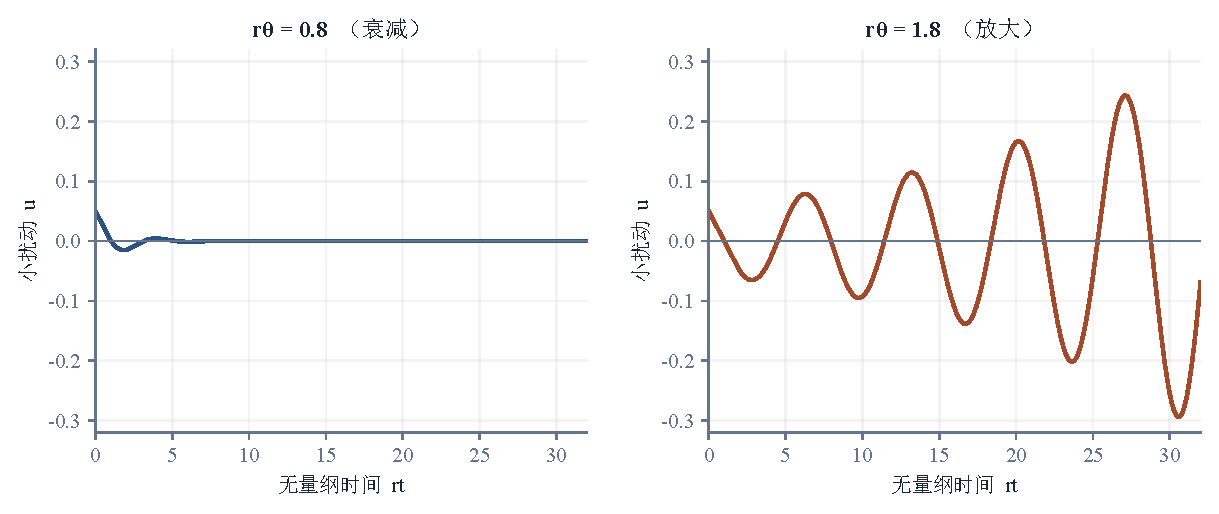
\includegraphics[width=\textwidth]{figures/delay-stability.pdf}
\caption{延迟逻辑斯蒂模型在正平衡点附近的线性化：$\dot u=-ru(t-\theta)$。以常值小扰动历史作数值示意，$r\theta=0.8$时扰动衰减，$r\theta=1.8$时振荡放大；第一条局部稳定边界为$\pi/2$。曲线展示线性局部行为。}
\label{fig:mechanism-delay-stability}
\end{figure}
\section{认知重塑与行动指南}

全书从一个落差开始：方案以推理速度出现，现实通过多只时钟改变。把这条转换链看清，才能知道下一次提速究竟改善了什么。

\subsection{走出图灵陷阱：能力、价值与资格分别判断}

行为测试可以检验指定接口上的能力。它的结果属于测试条件，不能替代对持续运行、权利与责任的全部判断。一个系统能写出答案，能稳定提供服务，能代表他人作决定，是三种不同要求。

人的价值也不等于某项产出的稀缺程度。能力扩展人的选择，报酬受需求、产权与议价影响，尊严则不能随一种交付物的市场价格一起折算。生成变便宜以后，社会仍然可以把新增能力用于健康、教育、照护、关系、探索与公共参与。

这里的“负熵体验者”强调两件事：人依赖实际条件维持生命，也在有限生命中体验、选择和建立关系。热力学说明维持的物理条件，伦理与制度说明怎样的生命值得被保护，二者各自提供理由。

价值重新落在哪里，需要观察新的接口。候选生成可能让位于审查；自动检查成熟以后，规范与任务定义又可能成为重点；部署扩大以后，维护、救济与分配可能更加紧迫。接口会移动，职业清单也会过时。

每个位置都要重新问：它建立了什么可依赖结果，凭据在哪里，换一种安排能否更好地完成同一功能，谁能进入这套安排。社会必要性不会自动兑现为工作机会和高报酬，培训、支付与权力配置必须同时处理。

\subsection{价值流向：跟踪稀缺的形成方式}

稀缺有不同来源。验证需要与任务相称的证据；照护需要时间、技能、可达性，有时也需要特定的人；现场判断需要信息、能力与实际处置权；长期教育需要让学生形成能力的路径。工具可以改善每一项，承担这些功能的结构也要随之更新。

评价不能只看名称。审计可能变成盖章，经验要求可能变成排斥，所谓陪伴也可能只剩服务话术。需要检查的是结果与形成路径：出了错能否发现，依据能否复核，承诺是否兑现，受影响者能否提出异议。

高价同样不是必要性的证明。市场稀缺可能来自真实供给约束，也可能来自垄断和人为门槛；重要工作则可能因为预算不足而长期低薪。价值流向的分析，要与分配分析并排进行。

这条规则可以反复重算：每次成本下降以后，辨认旧凭据失去了什么区分力，新凭据需要通过什么过程形成，以及谁掌握形成过程。技术可以创造实际使用价值，也可以重排价值证明的位置；具体收益由完整结果判断。

\subsection{降阻之前的三问}

\textbf{被降掉的是什么？}先固定任务、质量、基准、时间与系统边界。起草变快是一项收益，获得可靠决定变快是另一项，需要分别取证。

\textbf{其他环节怎样变化？}检查复核、返工、能源、设备、支持、风险与恢复。成本可能转移，也可能净下降，还可能出现新的支出。不能预先假定每次降阻都必须在别处原样偿还。

\textbf{谁获得收益，谁承担余账？}把用户、劳动者、运营者、受影响第三方与未来义务列入比较。总成本下降，也可能伴随不均等的收益和负担。

对软件团队，三问把生成连接到审查、回归风险与维护。对临床服务，它把模型表现连接到具体用途、医师义务、患者权利与随访。对运营车队，它把车辆效率连接到空驶、覆盖、设施与事故处置。答案应当具体到能够改变方案。

审查过载，就比较候选筛选和处理能力；故障无法收束，就缩小作用范围或重做恢复；责任没有落点，就先建立可追问与可补偿的安排。表格只记录这些决定，实质检查仍须有人有能力、有时间并有权执行。

\subsection{保留能生产能力的接口}

个体可以保留一部分直接练习，使自己仍能理解、检查与修订所依赖的结果。学习语言时先写再改，维护代码时实际阅读和测试，学习判断时接触结果并解释失败。好的工具可以让练习更有效。

保留多少由任务决定。某些能力需要持续暴露，某些偶尔练习即可维持；有些旧步骤已经不再产生学习，应当删除。目的在能力，而不在展示手工、吃力或不用工具的身份。

个人条件也不同。时间、残障、照护、收入与疲劳改变可选安排，辅助工具往往正是在高障碍处扩大自主。组织不能一面只考核即时产出，一面要求劳动者在私人时间无偿保存所有长期能力。

组织需要维护的是复核与重建过程的能力：相称的记录、胜任的审查、独立质疑，以及真正能执行的中断和纠正权。这些功能需要角色、预算与权限，不能用一句“谨慎使用”替代。

\subsection{让承担者保有有效位置}

受影响者需要知情、参与、代表与救济。有些决定可由本人同意，有些需要专业职责、公共程序或对脆弱群体的保护。决策权要与能力和控制相称，承担损失的人则需要实际可用的质疑和补偿路径。

下一代工具会改变许多具体答案。这套方法仍可继续使用：辨认介质，分开约束，追踪行动，检查反馈，核对整本账。能力越强，越需要知道它通过什么路径成为现实。

\section{负熵远征}

下一代机器可以让答案更容易获得。文明仍要决定维持什么、发现什么，以及准备让谁承担什么代价。

“负熵”首先提醒一项物理事实：生命与工程系统可以使用资源、输出熵流，维持局部组织。它在这里也承载一层人的愿望：把新增能力用于值得持续的世界。物理账本说明维持的条件，不能替我们选择值得维持的状态。

\subsection{形成与维持}

复制给出了一个小而明确的例子。若$\varepsilon_0$为初始每位错误率，校对与修复的条件性残余因子分别为$f_{\text{校对}}$和$f_{\text{修复}}$，在可以采用乘法组合的模型中，
\begin{equation}
\varepsilon_{\text{总}}=\varepsilon_0f_{\text{校对}}f_{\text{修复}},
\qquad
\mathbb E[M]=\varepsilon_{\text{总}}L .
\end{equation}
$M$为长度$L$上的错误数。期望错误数不等于至少发生一次错误的概率；保真度还依赖位置、上下文、相关性与修复机制。\cite{kunkel2000dna}

关键问题是：什么过程让结构在反复调用中保持可用。生物校对、程序测试、档案与机构复核采用不同机制，各自要核算成本和效果。

麦克斯韦妖把信息与物理边界之间的关系推得很深。信息可以引导操作，但循环的完整账本包括测量、存储与复位。兰道尔界限约束相应条件下的信息擦除，Bennett则梳理了计算、可逆性与妖的热力学。\cite{landauer1961,bennett1982thermodynamics} 把存储与热库放在图外，一次聪明操作就可能显得免费。

同样的遗漏也会发生在AI接口。候选便宜，可能因为准备已被摊销、候选可以撤回，或确认发生在别处。这些都是真实技术优势。最终价值要看它们使怎样的完整过程成为可能。

\subsection{丰裕扩大选择}

文明可以用智能改善健康、基础设施、教育、发现与生态，也可以用它加剧注意力竞争，或把某个狭窄目标优化得极其充分。去向由产权、激励、公共安排、组织与个人项目共同塑造。

舒适在这幅图里有正当位置。减轻疼痛、重复劳动、排斥与无用等待，都是进步。生活还需要关系、好奇、自主投入，以及判断能够得到回应的地方。

高阻力前沿提供一部分这样的相遇。一次艰难实验，一套被持续维护的公共服务，一片逐步恢复的生态，一个人的成长，一段关系，一门学到足以判断工具的手艺，也提供同样的入口。规模不同，要求相通：结果要通过行动和后果建立。

\subsection{在约束中扩大自由}

自由需要可用的可能性，对相关边界的理解，以及足以作选择的权力和支持。好的工程降低资源障碍、改善过程、隔离依赖、提高测量并建立恢复路径；好的制度处理新增收益和剩余代价怎样分配。

智能的规模让这项工作更加紧迫。候选便宜以后，选择的质量更重要；行动加快以后，反馈的匹配更重要；作用范围扩大以后，授权和责任更重要。

负熵远征，就是把新增可能变成值得持续的世界。它需要强大的搜索，需要能够行动的身体与机器，需要足以打断说法的证据，也需要愿意承担长期账本的人和机构。

智能寻找路径。文明由它建成的路径、持续看见的后果，以及这些路径使之成为可能的生活塑造。

\furtherreading{%
薛定谔《生命是什么》（Cambridge University Press, 1944）\\
冯·诺依曼《自复制自动机理论》（Burks 编，University of Illinois Press, 1966）\\
Nicholas Negroponte《数字化生存》（Alfred A. Knopf, 1995）\\
William F. Ogburn《社会变迁》（B. W. Huebsch, 1922）\\
William J. Baumol and William G. Bowen《表演艺术：经济的困境》（Twentieth Century Fund, 1966）\\
兰道尔《不可逆性与计算过程中的热产生》（IBM Journal of Research and Development, 1961）\\
Markus Reiner《德博拉数》（Physics Today, 1964）\\
香农《通信的数学理论》（Bell System Technical Journal, 1948）}


\appendix
%% ===================== 本章参考文献 =====================
\printbibliography[heading=subbibliography,title=参考文献]

\chapter{理论引擎：广义黏滞的物理基础与实证路线}
\markboth{附录 A\quad 理论引擎}{}

本书正文以机制叙述为主，公式只在必要处出现。这个附录把散在各章的物理依据集中起来，交代它们的学术来源、数学形式、可检验的推论和适用限度。它的目的是让前面那些看起来像是类比的表述，落回到可以被检查和被反驳的位置上。

\section{学术谱系与理论增量}

先说清楚本书的想法从哪里来，以及相对于已有论述增加了什么。关于技术与社会之间速度不匹配的判断并不新，它有一批各自独立、只在局部重叠的来源，本书的贡献不在于提出这个现象，而在于把它统一到一组可以参数化的约束上。

第一条来源是比特与原子的区分。Nicholas Negroponte 在《数字化生存》里用 bit 和 atom 的对立来描述数字化的边界，指出可以被数字化的东西和必须保持物质形态的东西遵循不同的规律。这个区分被广泛引用，但在他那里主要用于描述商业形态的变化，没有给出两种介质为什么不同的机制说明。\cite{negroponte1995being} 本书把它推进了一步：比特、原子与生命的差别不是形态差别，而是吸收机制差别：信息被转译为扩散，物质被转译为做功，生命被转译为反馈。三种介质的中文名称与英文对照为比特（Bits）、原子（Atoms）、生命（Gene），最后一个取遗传信息之意，而不指细胞里那段具体的遗传物质。这个推进带来一个可检验的推论：同一项智能技术进入三种介质时，其效果的时间曲线形状不同，扩散型是单调趋近，做功型受通量上限约束，反馈型会出现非线性甚至反向。

第二条来源是文化滞后。William F. Ogburn 在 1922 年提出，社会的物质文化变化快于非物质文化，两者之间的时间差造成失调，他把这个现象称为文化滞后。\cite{ogburn1922social} 这个概念抓住了问题的形状，但缺乏度量：什么是“快”，什么是“慢”，差别多大会产生失调，都没有给出可操作的量。本书用时间刚性 $T$ 给出度量，把“滞后”还原为两个过程的弛豫时间之比，从而把定性的判断变成可以比较的量。

第三条来源是生产率悖论。Robert Solow 在 1987 年的一句话被反复引用：计算机时代无处不在，唯独在生产率统计里看不到。\cite{solow1987watch} 此后三十年的研究大致收敛到一个结论：信息技术确实提高了生产率，但存在显著的滞后，而且滞后的长短取决于组织是否完成了配套的流程重组。这个结论与本书的拓扑耦合 $G$ 是同一件事的两种说法：技术进入系统后，产出不会立刻变化，因为系统需要重新布线，而重新布线的速度由组织结构和制度安排决定，不由技术本身决定。

第四条来源是成本病。Baumol 和 Bowen 在 1966 年对表演艺术的研究是这一说法的来源：在这类活动上，产出受制于现场的人力投入，效率提升的空间有限，当其他部门的工资随生产率上升时，它们的单位成本会被动抬高；这个概念后来被推广到教育、医疗与照护等同样难以提速的领域。\cite{baumol1966performing} 它抓住的是价格信号，不匹配会以相对价格分化的形式被经济系统记录下来，而这一点可以直接从产业统计里观察到。本书接上的是它没有回答的那一环：这些位置为什么难以被其他机制替换。答案是时间刚性与拓扑耦合，它们不随算力下降，因此这类相对价格不会因为生成能力普及而回落。两种判断落在同一批对象上，依据不同，合起来比单独使用更可靠。

这些来源分别处理数字化、时间差、组织互补和相对成本，已有各自的度量与模型。这里提出的工作，是用资源、时间与耦合组织同一条现实转换链，继续把验证和责任列入比较。评价标准是它能否增加解释、区分方案并改善决定。

相对于这四条来源，本书的理论增量可以归结为三点。一是把三种阻力统一成一组参数 $(R, T, G)$，使不同类型的黏滞可以在同一个框架下比较和置换。二是给出介质的分类，说明同样是智能输入，进入不同介质后被吸收的方式不同，因此不能用同一套加速逻辑处理。三是把验证与承责纳入约束，作为与物理阻力并列的一类黏滞。第三点是本书与前人差别最大的地方，也是最需要被检验的地方。

这四条来源各自还带着一层本书没有采纳的判断，把它们分清楚可以避免误读。文化滞后理论在提出者那里常常带有对传统的肯定意味，而本书只取其中的时间差结构，不取任何关于快慢孰优的结论；成本病理论常被用来论证某些部门效率低下，而本书只取相对价格上升的机制，不取对部门本身的评价；生产率悖论在早期被当作技术无效的证据，后来被当作滞后即将结束的乐观预期，本书对两种读法都不采纳，只保留技术效果需要配套重组这一条；比特与原子的区分常被用来判断哪些行业会被数字化，本书不取这一层预测用法，只取两种介质吸收机制不同这一条。做这样的切割是有代价的：能说的话变少了，能被误用的地方也变少了，而一个框架的可信度主要取决于后一条。

需要补一句关于增量的性质的话。这三点都属于形式上的统一，不属于新机制的发现：参数化的价值在于让不同领域的观察可以在同一张表上比较，而不在于提出了某个此前无人知道的机制。因此对本书的评价标准也应当相应调整：不应当问它是否发现了新的物理，而应当问它给出的这组参数是否真的能区分不同的情形，以及用它做出的推论是否可以被证伪。

\section{广义黏滞方程的数学架构}

正文第二章给出了广义黏滞系数 $\eta = f(R,T,G)$，并在第 2.5 节末写出了指数形式 $\eta=\eta_0\exp(\alpha R+\beta T+\gamma G)$ 与三个系数各自的含义；那里没有展开的，是这个形式为什么取指数、三项为什么可乘、以及它落到可检验命题上还缺什么。这一节补的正是这三件事，同时说明这个形式的地位：它是一组待检验的假设形式，不是已经被确证的关系。

\subsection{内禀黏滞指数法则}

假设在固定任务与测量口径下，三类约束对对数转移代价的边际影响近似恒定，且暂不计入交互项，那么总黏滞系数可以写成

\begin{equation}
\eta = \eta_0 \exp\left(\alpha R + \beta T + \gamma G\right)
\end{equation}

式中 $\eta_0$ 是基准黏滞系数，取值取决于所讨论的环节本身，与三类约束无关；$R$、$T$、$G$ 分别是资源势垒、时间刚性和拓扑耦合的归一化度量，量纲为一；$\alpha$、$\beta$、$\gamma$ 是三个常数，表示各类约束的相对权重，其数值需由实证确定，预期均为正。指数形式的来源是：如果每一类约束按比例降低通过速率，而多类约束同时作用时降低倍率相乘，则总倍率的对数等于各类约束的线性叠加。这个形式与阿伦尼乌斯方程中速率常数对活化能的指数依赖属于同一族，其共同点是处理“需要通过一个障碍”的过程，而不是处理“在平坦空间中移动”的过程。

指数中的可加性，等价于相对代价倍率可乘。它要求$\partial\ln\eta/\partial R=\alpha$等边际关系在考察区间内近似不变。物理串联过程的历时可以相加，稳态管线的吞吐也可能由最慢环节限制，不能仅凭“串联”推出倍率相乘。出现交互作用时，可检验$\delta RT$等扩展项；采用哪种形式，要比较解释与样本外表现。

测量先固定一个结果口径。$\eta=C/C_{\mathrm{ref}}$中的$C$可以取费用、总工时或单位合格结果的平均通过时间，$C_{\mathrm{ref}}>0$取同任务的公开参照。成功率与代价的方向相反，若采用成功率作代理，需要先规定相应变换。测量基准确定以后，$\alpha$才可读为资源约束增加一单位时对数代价的边际变化。不同研究的变量、边界和参照一致，系数才有可比性。

三个自变量需要各自公开定义、基准与取值方式。归一化可以采用同类需求与可用能力的比值，或采用可重复的连续指标；0到5级的等级表则先用于序数判断。自变量应尽量由转移前的条件或独立资料构造，避免把待解释的费用与历时换名后再次作为解释变量。跨研究合并前先核对任务、刻度和边界，再比较系数与残差。

这个形式可以提出三类检查：残差是否仍按任务或介质呈现结构，参数能否在可比样本中复现，交互与阈值形式能否更好地解释观察。指数函数的边际支出平滑增长，并不自动产生相变或突变阈值。模型形状与具体临界机制需要分别建立。

等黏滞面上的置换比可以写成，

\begin{equation}
\left(\frac{\partial R}{\partial T}\right)_{\eta}=-\frac{\beta}{\alpha}
\end{equation}

式中，$R$ 为资源势垒的归一化度量，$T$ 为时间刚性的归一化度量，两者量纲为一；$\alpha$ 与 $\beta$ 分别为 $\ln\eta$ 对 $R$ 与对 $T$ 的偏导数，量纲为一；下标 $\eta$ 表示在黏滞系数保持不变的条件下取值。这个式子的含义是：要让黏滞保持不变，资源约束每放松一个单位，时间约束沿等值面收紧$\alpha/\beta$个单位，反之亦然，这正是正文所说的三组约束可以相互置换的定量形式，即压缩时间要投入更多资源、节省资源要拉长时间。适用条件必须写明：$\alpha$、$\beta$ 的数值须由实证确定，本式只给出置换比的结构；它成立的前提是可乘假设；一旦这个前提失效，就需要在指数上补一个交叉项，置换比随之不再是一个常数。

三条含义中，第一条最容易被误读。残差没有结构是模型成立的必要条件，不是充分条件：一个错误的模型也可能在小样本上给出无结构的残差。因此这条检验必须以介质为分组单元来做，而不是把不同介质的数据混在一起拟合；混在一起时，介质的差异会被吸收进残差，看起来像噪声，实际上是被忽略的变量。这一点决定了附录第三节的检验路线为什么必须按介质分别设计。

参数的跨期稳定性需要样本外检查。漂移可能来自技术变化、边界改变、变量定义或遗漏条件，不能据此直接判定因果方向反转。应保留定义与版本，比较替代解释，并说明模型在什么区间仍有预测能力。

还有一点关于自变量的写法需要交代。三类约束各自内部可能包含若干不同的成分，例如资源约束里既有材料的可得性也有资金的可得性，而公式里只允许出现一个数。把多维的约束压成一个标量，意味着研究者要先确定用什么方式汇总，例如取各项的最大值，或者按某个权重求和，而这个汇总方式与三个系数一样需要写明。汇总方式选得不好，误差会进入残差并被当成噪声；如果选得好，残差应当回到随机水平。这条要求不增加新的假设，它只是承认一件本来就必须回答的事：任何一个只允许输入一个数的形式，都要先交代这个数是怎么来的。

\subsection{社会技术德博拉数}

第二组形式处理的是“同一个系统在不同观测尺度上表现为固体还是流体”的问题。德博拉数来自流变学，由 Markus Reiner 在 1964 年提出，定义为材料的弛豫时间与观测时间尺度之比。\cite{reiner1964deborah}

\begin{equation}
\mathrm{De} = \frac{\tau_{\text{relax}}}{\tau_{\text{obs}}}
\end{equation}

$\tau_{\text{relax}}$ 是系统内部结构重新调整所需的时间，$\tau_{\text{obs}}$ 是观察者关心这件事的时间尺度，两者同量纲，因此 $\mathrm{De}$ 无量纲。$\mathrm{De} \ll 1$ 时，系统在观测尺度内完成调整，表现为可以流动的流体；$\mathrm{De} \gg 1$ 时，系统来不及调整，表现为固体的弹性响应。用一个具体例子说明它的用法：一项技术对就业的影响，如果以季度为观测尺度（$\tau_{\text{obs}}$ 小），则 $\mathrm{De}$ 很大，系统表现为刚性，短期内劳动者无法转岗；如果以二十年为观测尺度，则 $\mathrm{De}$ 变小，同一系统的流动性显现出来。两种判断都不错，它们描述的是同一个系统在不同尺度上的行为，而争论常常发生在双方使用了不同的 $\tau_{\text{obs}}$ 却没有说明。

若系统近似满足单弛豫时间的Maxwell响应，周期输入下的损耗模量在角频率与弛豫时间之积接近1时达到峰值。将这种判断用于组织，需要先识别相应的周期输入与恢复机制。季度和二十年的观察窗可以改变对调整快慢的描述，本身不会改变系统的实际吸收成本。治理若要降低失配，应改变响应能力、输入频率或缓冲结构；延长统计窗口只改变观察口径。

这个名字的来源值得一提，因为它点出了这个量的适用范围。Reiner 取自《士师记》中底波拉之歌的一句“山在耶和华面前流动”，用来说明同一物质在足够长的时间尺度上可以表现出流动，而在短尺度上表现出固体。这个出处说明德博拉数从一开始就是一个关于尺度对比的量，而不是关于材料类别的量；它不把系统分成刚性的和流动的两类，只回答“在当前的观测窗里，它来得及调整吗”。因此它在本书里的用法也应当照此理解：给某个社会技术系统贴上“刚性”或“有弹性”的标签是没有意义的，有意义的说法是指明观测窗。

这个量在本书中有一个直接的用处：它把“技术性失业是短期的还是长期的”这类争论还原为一个可计算的问题：$\tau_{\text{relax}}$（劳动力市场的重组时间）与 $\tau_{\text{obs}}$（政策关心的时间窗）的比值。争议因此不再关于立场，而关于两个可以被测量的时间常数。同样的还原可以用在其他争论上：关于某项技术“来不及治理”的判断，实际上是说 $\tau_{\text{relax}}$ 大于治理机制的响应时间；关于某项制度“很有韧性”的判断，实际上是说它的响应时间短于它需要吸收的扰动的周期。两种说法都可以被具体的测量替代，而一旦被替代，争论就从立场转到数据。

$\tau_{\text{relax}}$ 在社会系统里同样需要一个可测的代理量，而这个代理量往往就是一个物理的周期。职业结构的重组速度受制于培养周期，一个需要十年上下才能完成训练并独立执业的职业，其人员存量不可能在一两年内改变，因此 $\tau_{\text{relax}}$ 至少是培养周期的量级。设备和基础设施的更新速度受制于折旧年限与建设周期，制度安排的调整速度受制于立法与复议的周期，这些都可以从公开文件里读出具体年数。把这几项里最长的一项当作 $\tau_{\text{relax}}$ 的下界估计，是一个粗糙但可用的起点，因为它只用到可以直接查证的年限，不需要对行为做假设。粗略估计已经足以支撑一类判断：当政策关心的时间窗短于这个下界时，任何关于结构已经调整完毕的结论都不成立，无论数据看上去多么支持它。

观测窗的选择本身带有立场成分，这一点需要承认而不是回避。同一项变化，以季度为窗口会得到需要立即干预的结论，以代际为窗口会得到属于正常调整的结论，而两种窗口都可以被论证为合理。承认这一点不会使这个量失效，原因在于 $\tau_{\text{relax}}$ 与窗口无关：它由系统的结构决定，不由观察者决定，因此争论可以收窄为窗口选择的问题，而窗口选择是可以被公开讨论和检查的。可操作的规范是：给出结论时同时写明所用的窗口，并说明在这个窗口下被略过了什么。做到这一条，不同窗口下的判断可以并存而不互相取消，它们各自指明了在自己那段时间尺度上必须处理的问题。

用这个量的时候还有一点容易被忽略：弛豫时间不是一个系统只有一个，而是一个机制对应一个。劳动力市场的重组、供应链的重建、法规的修订、设备存量的更新，各有自己的时间常数，彼此可以相差很多，因此说某个系统的德博拉数是多少，必须连同机制一起说明。在实践里可以这样做：把关心的问题拆到具体机制上，为每一项给出自己的时间常数，再判断哪一项与观测窗最接近。与观测窗最接近的那一项，通常就是决定结论的那一项。同一件事在不同研究里会得到不同的判断，因为它们关心的机制不同。

\subsection{剪切增稠}

第三组形式处理的是“施加得越快，系统越硬”的现象。正文第四章讨论生物干预时使用了这一形式，其一般表达为幂律

\begin{equation}
\eta(\dot\gamma) = \eta_b + k\,\dot\gamma^{\,n},\qquad n > 0
\end{equation}

其中 $\dot\gamma$ 是剪切速率，量纲为时间的倒数，在这里对应干预施加的速率；$\eta_b$ 是零剪切黏滞，对应系统在缓慢干预下的响应，记作 $\eta_b$ 是为了与本附录前一节广义黏滞式里的基准黏滞系数 $\eta_0$ 区分开；$k$ 是增稠系数，$n$ 是幂指数。$n > 0$ 表示施加越快、等效黏滞越高，即系统以更强的抵抗回应更快的干预，$n$ 越大上升越陡。这个形式对生物系统特别适用，因为活系统有主动的代偿机制：干预速率超过代偿响应速率时，系统不会被动接受，而会启动反向调节，表现为表观阻力上升。

与它相对的是剪切变稀，即幂指数取负值或使用饱和形式的情形：施加越快，系统越容易流动。两种行为在流变学里都被研究得很清楚，区别在于系统的微观结构在剪切下是被拆散还是被组织起来。把这两个方向都写出来，可以避免一种常见的误读，即把“阻力随速率上升”当成所有复杂系统的普遍规律。真实的情形是按速率分段的：在低速区系统可能有足够时间重组，表现为剪切变稀；超过某个速率之后代偿跟不上，转变为剪切增稠。第四章讨论的干预强度阈值，对应的正是这个转折点。

按速率分段这件事有一个可以指认的机制：代偿需要时间，代偿机制的响应速率决定了转折点的位置。干预速率低于代偿速率时，系统来得及把扰动吸收掉，表现为阻力不随速率上升甚至下降；干预速率超过代偿速率时，代偿本身开始被扰动打乱，系统只能用更强的抵抗回应，表观黏滞转为上升。所以转折点不是某个固定的阈值，而是 $1/\tau_{\text{compensation}}$ 量级的速率，其中 $\tau_{\text{compensation}}$ 是该系统代偿环节的响应时间。这个读法把剪切变稀与剪切增稠统一成同一个系统在不同速率下的两种表现，而不是两类不同的系统，它与德博拉数处理尺度问题的思路一致：一个量比值决定看到哪一种行为。它同时给出一个可检验的推论：如果人为延长某个系统的代偿时间，例如削弱其调节能力，那么转折点应当向更低的干预速率移动，曲线的低速率段也会相应缩短。这个推论在细胞、组织和社会组织三个层次上都可以设计实验来检验，检验的结果决定这一节的形式还能不能继续外推。

流变学里这类行为之所以可以被当作定律使用，是因为它的机制被查清过。以高浓度颗粒悬浮液为例，剪切速率提高到一定程度后，颗粒来不及沿流线重新排列，被迫形成瞬时的聚集结构，流动阻力随之跳升，玉米淀粉浆在快速搅动下变硬就是这一机制的直接表现。这里的关键不在于现象引人注意，而在于现象的来源可以被独立验证：通过流变测量与散射实验能够确认聚集结构的存在，因此幂律中的指数与起始速率都可以被赋予机制上的解释。本书把这个形式移到生物与制度系统时，缺少的正是这一步独立验证，现有的依据是形状相似，而形状相似本身不足以支撑借用。所以这一节的地位必须写明：它给出的是一个待检验的外推，检验的标准是能否在目标系统里指出与聚集结构相对应的机制。

如果要在生物与制度系统里找这个形状的候选，判断的线索是：系统是否有一个需要时间的调节回路，以及这个回路是否会在输入过快时被自身打乱。抗生素使用强度上升与耐药率上升之间的关系、耕作强度上升与地力下降之间的关系、考核频次上升与被考核行为失真之间的关系，都属于这一形状的候选，它们的共同点是调节机制在高强度输入下反而成为扰动的一部分\cite{laxminarayan2013antibiotic}。列出这些候选不等于确认它们，每一例都需要单独的实证工作：测量起始强度、测量曲线的斜率、确认调节回路的存在。把候选与结论分开写，是为了避免一种常见的错误，即用一个领域里已经成立的机制，去为另一个领域里仅仅形状相似的曲线提供担保。

速率继续上升以后，系统可能饱和、失稳、损伤或堵塞，转折由具体机制决定。幂律只描述测量覆盖的区间。报告需要列出速率跨度、重复测量与转折迹象，并比较幂律、阈值或饱和形式在更宽区间的表现。高剪切率行为不能由拟合区间内的指数单独决定。

辨识幂律需要足够宽的输入区间和重复测量。基准项$\eta_b$不可忽略时，$\ln\eta$对$\ln\dot\gamma$的斜率不恒等于$n$，应拟合完整表达式，或说明在哪个区间可以忽略基准。还应比较阈值与饱和形式，并报告区间外转折。

三组形式的地位并不相同。指数法则和德博拉数是描述性的工作假设，其形式由机制的类比推得，参数需要实证确定；剪切增稠幂律在流变学中有扎实的实验基础，本书把它移到生物和制度系统上是一个有待检验的外推。把三者的地位分清，是为了避免一种常见的错误：把一个在一个领域内被验证过的形式，当作在所有领域内都成立的定律来使用。

\section{定性判据：无参数条件下的使用方式}

参数尚未标定时，框架先用于定位约束、进行有条件的比较和选择需要测量的环节。定性判断依靠公开证据与明确的序关系。能够判断的方向直接报告，存在权衡而证据不足的情形则保留为待比较的方案。

\subhead{定位：把对象放进三个坐标}

把一个对象放进 $(R,\,T,\,G)$ 三个坐标里，得到的不是一组数值，而是一个位置：它在三个维度上分别处在低、中、高哪一档。这一档的判断通常不需要测量，只需要回答表 \ref{tab:ch2-rtg} 列出的三个问题：推得动推不动、来得及来不及、传得开传不开。做完之后，对象就被分到了介质梯度的某一级上。

这种分类的操作性在于判据是公开的。两个人对同一个对象给出不同的档位，可以直接检查各自依据的是哪一条证据，而不必先争论一个数字谁更准。相比之下，“这项技术的黏滞系数是 3.7”这样的陈述无法被追究，因为没有人能说清 3.7 是从哪一步来的。模糊的档位在这件事上反而更硬：它逼着每一个判断落到一条可以指出来的证据上。

\subhead{分区：八个区域与各自的处理方式}

三个坐标各有 0 到 5 级，以中点 2.5 级为界，0 到 2 级记低，3 到 5 级记高。三个坐标各自或低或高，空间就被切成八个区域；判断一个对象落在哪一区，只需要回答三个是否：资源势垒是否过了中点，时间刚性是否过了中点，拓扑耦合是否过了中点。这个判断比定级更粗，因而也更稳，两个人即使在同一坐标上相差一级，只要没有跨过中点，得到的区域仍然相同。

区域的命名由高的坐标拼成。只有一个坐标高，就以它命名：资源高叫资源锁，时间高叫时间锁，耦合高叫耦合锁。两个坐标高，把两个名字连起来：资源与时间高叫资源时间，时间与耦合高叫时间耦合，资源与耦合高叫资源耦合。三个都高叫三重锁，三个都低叫低黏滞区。第六章按字面用过“低黏滞区”这个词，这里给它一个确切的边界。

\begin{figure}[ht]
\centering
% 原图自然宽度 13.40 cm，放大到 14.30 cm 以接近版心宽度
\scalebox{1.067}{% >>>>>>>>>> figs/fig-rtg-octant.tex >>>>>>>>>>
% 图 A-1  广义黏滞空间的三维分区与技术落位
%
% 投影：斜二测。R 向右、T 向上、G 向左上后退，均为线性映射
%   x = ox + L*(R - kx*G),  y = oy + L*(T + ky*G)
% 只画三个朝向读者的面：G=0 的前面、T=5 的顶面、R=0 的左面，共 12 个小
% 四边形。不可见的棱一律不画：唯一被挡住的顶点是 (5,0,5)（在图中投到
% (ox+1.368, 2.256)），从它引出的三条棱都在框体背后。把棱画成虚线会在
% 框内留下与中位线近于平行的第二条线（D 到 (5,0,5) 的棱与前面 T=2.5 的
% 中位线只差 0.14 cm），读者会误当成分区线，因此整体省略。
%
% 分区：三个坐标各以 2.5 级为界（即等级 0-2 记低、3-5 记高）。三个中位面
% 把空间切成八区。12 个小四边形按所属区域着色，深浅（色相）表示该区有
% 几个高坐标：绿 0、灰 1、棕 2、红 3。每个小四边形的名字由高坐标拼成，
% 例如 R 与 T 高称「资源时间」。
%
% 八个区域里有七个能在可见面上找到自己的格子：前面四格是 G 低的四区，
% 顶面四格是 T 高的四区，左面四格是 R 低的四区（四格重合于中位面两侧的
% 区）。剩下的一区是资源耦合（R 高、T 低、G 高），它朝向背面，没有可见
% 面，图中不画，由图注交代。
%
% 落位：每个技术点画在它自己的 (R,T,G) 上，再引一条细虚线连到它所属区域
% 在可见面上的落点（实心小点）。落点必定落在与其同区的格子里，于是「点
% 在哪一区」可以一步读出。规则：T 高就直上到 T=5，否则 G 低就沿 G 退到
% G=0，两者都不满足的点本身已经落在可见面上。
\begin{tikzpicture}[x=1cm, y=1cm, font=\small,
  ax/.style={-{Stealth[length=2.0mm]}, ink, line width=0.7pt},
  edge/.style={slate!75, line width=0.5pt},
  mid/.style={slate!55, line width=0.35pt, dash pattern=on 1.2pt off 1.1pt},
  stem/.style={line width=0.45pt, dash pattern=on 1.5pt off 1.1pt},
  foot/.style={circle, fill, inner sep=0.52pt},
  tick/.style={font=\tiny, text=slate, inner sep=0pt},
  rlab/.style={font=\scriptsize\heiti, inner sep=0pt},
  dlab/.style={font=\scriptsize\heiti, inner sep=0pt},
  clab/.style={font=\scriptsize\heiti, text=ink, inner sep=0pt},
  lead/.style={slate!75, line width=0.35pt},
  dom/.style={circle, inner sep=1.75pt},
  % 链上单元：实心圆，颜色取所属区域的深色
  ug/.style={circle, fill=forest, draw=white, line width=0.6pt, text=white,
             font=\tiny, minimum size=3.4mm, inner sep=0pt},
  ut/.style={circle, fill=terra, draw=white, line width=0.6pt, text=white,
             font=\tiny, minimum size=3.4mm, inner sep=0pt},
  ur/.style={circle, fill=rust, draw=white, line width=0.6pt, text=white,
             font=\tiny, minimum size=3.4mm, inner sep=0pt},
  um/.style={rounded corners=1.2pt, fill=forest, draw=white, line width=0.6pt,
             text=white, font=\tiny, inner sep=1.3pt},
  % 界面单元：空心圆，只有一圈彩色描边
  ii/.style={circle, fill=white, draw=terra, line width=0.8pt, text=terra,
             font=\tiny, minimum size=3.4mm, inner sep=0pt}
]
\useasboundingbox (-0.34,-0.72) rectangle (13.06,6.45);

% ================= 箱体：可见面着色、中位线、棱、坐标轴 =================
\newcommand{\boxat}[1]{%
  \coordinate (A) at ({#1},{0.60});
  \coordinate (B) at ({#1+3.60},{0.60});
  \coordinate (C) at ({#1},{4.20});
  \coordinate (D) at ({#1-2.232},{2.256});
  \coordinate (E) at ({#1+3.60},{4.20});
  \coordinate (G) at ({#1-2.232},{5.856});
  \coordinate (H) at ({#1+1.368},{5.856});
  % ---- 前面（G=0）切成四块 ----
  \fill[forest!16] (A) rectangle ({#1+1.80},{2.40});
  \fill[slate!17]  ({#1+1.80},{0.60}) rectangle ({#1+3.60},{2.40});
  \fill[slate!17]  ({#1},{2.40}) rectangle ({#1+1.80},{4.20});
  \fill[terra!19]  ({#1+1.80},{2.40}) rectangle (E);
  % ---- 左面（R=0）切成四块 ----
  \fill[forest!16] (A) -- ({#1},{2.40}) -- ({#1-1.116},{3.228}) -- ({#1-1.116},{1.428}) -- cycle;
  \fill[slate!17]  ({#1},{2.40}) -- (C) -- ({#1-1.116},{5.028}) -- ({#1-1.116},{3.228}) -- cycle;
  \fill[slate!17]  ({#1-1.116},{1.428}) -- ({#1-1.116},{3.228}) -- ({#1-2.232},{4.056}) -- ({#1-2.232},{2.256}) -- cycle;
  \fill[terra!19]  ({#1-1.116},{3.228}) -- ({#1-1.116},{5.028}) -- ({#1-2.232},{5.856}) -- ({#1-2.232},{4.056}) -- cycle;
  % ---- 顶面（T=5）切成四块 ----
  \fill[slate!17]  (C) -- ({#1+1.80},{4.20}) -- ({#1+0.684},{5.028}) -- ({#1-1.116},{5.028}) -- cycle;
  \fill[terra!19]  ({#1+1.80},{4.20}) -- (E) -- ({#1+2.484},{5.028}) -- ({#1+0.684},{5.028}) -- cycle;
  \fill[terra!19]  ({#1-1.116},{5.028}) -- ({#1+0.684},{5.028}) -- ({#1-0.432},{5.856}) -- ({#1-2.232},{5.856}) -- cycle;
  \fill[rust!17]   ({#1+0.684},{5.028}) -- ({#1+2.484},{5.028}) -- ({#1+1.368},{5.856}) -- ({#1-0.432},{5.856}) -- cycle;
  % ---- 可见面上的中位线 ----
  \draw[mid] ({#1+1.80},{0.60}) -- ({#1+1.80},{4.20});
  \draw[mid] ({#1},{2.40}) -- ({#1+3.60},{2.40});
  \draw[mid] ({#1-1.116},{1.428}) -- ({#1-1.116},{5.028});
  \draw[mid] ({#1},{2.40}) -- ({#1-2.232},{4.056});
  \draw[mid] ({#1+1.80},{4.20}) -- ({#1-0.432},{5.856});
  \draw[mid] ({#1-1.116},{5.028}) -- ({#1+2.484},{5.028});
  % ---- 可见的棱：外轮廓六边形与中间的三条 ----
  \draw[edge] (A) -- (B) -- (E) -- (C) -- cycle;
  \draw[edge] (E) -- (H) -- (G) -- (C);
  \draw[edge] (G) -- (D) -- (A);
  \draw[edge] (D) -- ({#1},{2.256});
  % ---- 坐标轴 ----
  \draw[ax] (A) -- ({#1+3.78},{0.60});
  \draw[ax] (A) -- ({#1},{4.38});
  \draw[ax] (A) -- ({#1-2.411},{2.389});
  \node[font=\scriptsize, text=ink, anchor=west] at ({#1+3.86},{0.60}) {$R$};
  \node[font=\scriptsize, text=ink, anchor=south east] at ({#1-0.05},{4.46}) {$T$};
  \node[font=\scriptsize, text=ink, anchor=east] at ({#1-2.50},{2.42}) {$G$};
}

% ================= (a) 八个区域与五个领域的落位 =================
\boxat{2.60}
\node[tick, anchor=north] at (2.50,0.48) {0};
\node[tick, anchor=north] at (6.20,0.48) {5};
\node[tick, anchor=east]  at (2.45,4.20) {5};
\node[tick, anchor=west]  at (0.44,2.08) {5};

% 区域名（颜色＝高坐标的个数；资源耦合没有可见面，由图注交代）
\node[rlab, text=forest] at (3.70,1.86) {低黏滞区};
\node[rlab, text=slate]  at (5.30,1.50) {资源锁};
\node[rlab, text=slate]  at (3.50,3.30) {时间锁};
\node[rlab, text=slate]  at (0.926,2.742) {耦合锁};
\node[rlab, text=terra]  at (5.30,3.30) {资源时间};
\node[rlab, text=terra]  at (0.926,4.542) {时间耦合};
\node[rlab, text=rust]   at (3.626,5.442) {三重锁};

% 五个领域：先画落位引线与落点，再画点，最后挂标签
\draw[stem, forest!80] (2.427,1.262) -- (3.32,0.60);
\node[foot, forest] at (3.32,0.60) {};
\draw[stem, rust!80] (2.974,4.805) -- (2.974,5.525);
\node[foot, rust] at (2.974,5.525) {};
\draw[stem, rust!80] (4.141,4.474) -- (4.141,5.194);
\node[foot, rust] at (4.141,5.194) {};
\node[dom, fill=forest] (d1) at (2.427,1.262) {};
\node[dom, fill=rust]   (d2) at (2.974,4.805) {};
\node[dom, fill=terra]  (d3) at (2.701,5.194) {};
\node[dom, fill=terra]  (d4) at (2.254,5.525) {};
\node[dom, fill=rust]   (d5) at (4.141,4.474) {};
\node[dlab, text=forest, anchor=west]  at (2.72,1.262) {大模型};
\node[dlab, text=rust,   anchor=west]  at (2.72,4.46)  {半导体};
\node[dlab, text=rust,   anchor=west]  at (4.32,4.40)  {脱碳};
\node[dlab, text=terra,  anchor=south] at (2.60,5.62)  {低空};
\node[dlab, text=terra,  anchor=south] at (1.66,5.90)  {基因编辑};
\draw[lead] (1.76,5.83) -- (2.19,5.56);
\draw[lead] (2.68,5.60) -- (2.70,5.30);

% ================= (b) 低空飞行器九个单元的落位 =================
\boxat{8.90}
\draw[stem, rust!80]   (9.721,3.754) -- (9.721,5.194);
\draw[stem, forest!80] (9.447,2.702) -- (10.34,2.04);
\draw[stem, forest!80] (9.174,1.651) -- (9.62,1.32);
\draw[stem, terra!80]  (9.001,3.754) -- (9.001,5.194);
\draw[stem, terra!80]  (7.834,4.805) -- (7.834,5.525);
\draw[stem, terra!80]  (7.388,5.136) -- (7.388,5.856);
\node[foot, rust]   at (9.721,5.194) {};
\node[foot, forest] at (10.34,2.04) {};
\node[foot, forest] at (9.62,1.32) {};
\node[foot, terra]  at (9.001,5.194) {};
\node[foot, terra]  at (7.834,5.525) {};
\node[foot, terra]  at (7.388,5.856) {};
\node[ur] at (9.721,3.754) {1};
\node[um] at (9.447,2.702) {2·3};
\node[ug] at (9.174,1.651) {4};
\node[ur] at (9.721,4.474) {5};
\node[ut] at (9.001,3.754) {6};
\node[ii] at (7.834,4.805) {7};
\node[ii] at (7.388,5.136) {8};
\node[ii] at (7.114,5.525) {9};
% 分类标签：实心＝链上，空心＝界面
\node[foot, ink, inner sep=0.62pt] at (9.28,3.16) {};
\node[clab, anchor=west] at (9.45,3.16) {链上单元};
\node[ii, minimum size=2.1mm, line width=0.9pt] at (7.02,6.14) {};
\node[clab, anchor=west] at (7.20,6.14) {界面单元};

% ================= 图例与栏标题（一律在内容下方）=================
\node[font=\scriptsize, text=slate, anchor=west] at (0.60,0.20) {高坐标的个数＝};
\foreach \i/\cc in {0/forest, 1/slate, 2/terra, 3/rust} {
  \pgfmathsetmacro{\gx}{3.10+0.90*\i}
  \fill[\cc] (\gx,0.11) rectangle ({\gx+0.20},0.31);
  \node[font=\scriptsize, text=slate, anchor=west] at ({\gx+0.30},0.21) {\i};
}
\node[anchor=north, font=\footnotesize\heiti, text=slate] at (3.28,-0.12)
      {(a) 八个区域与五个领域的落位};
\node[anchor=north, font=\footnotesize\heiti, text=slate] at (9.58,-0.12)
      {(b) 同一领域内部九个单元的落位};
\end{tikzpicture}

% <<<<<<<<<< figs/fig-rtg-octant.tex <<<<<<<<<<
}
\caption{三个坐标与八个区域。图中点位为分类方式的示意，展示单元与区域怎样对应；它们不构成实测行业评分、总体黏滞排序或投运时间预测。具体项目应按表\ref{tab:scale-five}的问题取证，并在同一判据下重新定位。}
\label{fig:rtg-octant}
\end{figure}

区域名中的“锁”表示当前任务面临的高约束，类别由所采用的量表确定。高约束是否可以放松，需要继续查明可替代资源、过程改造和结构重组的条件。分区先标出检查重点，处理方案再按证据选择。

低黏滞区的三个坐标均低，通常较少遇到这三类障碍。实际扩张仍取决于需求、可靠性和组织能力，分区本身不提供增长速度。

单锁区先检查主导约束：能否通过替代资源、改变过程或缩小依赖面来降低它。绕行是一种候选策略，其代价和可行性须与直接改造比较。

双锁区需要同时检查两项约束及其联动。两个坐标都高，不排除某项改进同时降低两者；改造节奏由可行路径、投入和验证要求决定。等值面斜率只描述给定模型中的代价组合。

三重锁区提示资源、时间和结构都需要重点核查。分阶段投入、重新定义任务或基础设施改造，都可能改变坐标组合。能否推进，需要检查项目的可行集合，不能由三项评分直接判定。

分区与定级是同一件事的两种精度。定级给出三个档次，分区给出一个格子；格子丢掉的是内部的差别，换来的是边界的稳定。代价也说清楚：靠近中点的对象会在两个区域之间摇摆，一次赋值的小改动就足以让它换区。这种摇摆不是缺陷，它对应现实中确实含混的情形，一项技术刚刚跨过中点时，说它“开始被卡住”和说它“还没被卡住”都不算错。

定位先定级、再定区，给出位置与需要优先核查的约束。下一节的量表把八个区域落到具体技术上。

\subhead{比较：共同改善与跨维权衡}

定位之后，两个对象的相对黏滞可以在不给权重数值的条件下比较出来。设两个状态 $a$、$b$ 在三个坐标上的差为 $\Delta R=R_{a}-R_{b}$、$\Delta T$、$\Delta G$，由内禀黏滞的指数形式两边取对数得

\begin{equation}
\ln\frac{\eta_{a}}{\eta_{b}}
=\alpha\,\Delta R+\beta\,\Delta T+\gamma\,\Delta G
\end{equation}

在参照与刻度一致、权重为正的条件下，若$a$的三个约束均不高于$b$，且至少一项更低，模型给出$\eta_a<\eta_b$。这是一种支配关系。若一项下降而另一项上升，只知道权重次序和变化符号通常不足以确定总效果，还需要权重比与变化幅度的界限。0到5级量表提供的是序数，代入指数模型之前，还须建立有意义的数量刻度。

\subhead{判方向：只需要导数的符号}

趋势判断需要的信息更少，只需要导数符号。对上式求时间导数，

\begin{equation}
\operatorname{sgn}\!\left(\frac{d\ln\eta}{dt}\right)
=\operatorname{sgn}\!\left(\alpha\dot{R}+\beta\dot{T}+\gamma\dot{G}\right)
\end{equation}

三个坐标同向变化且权重为正时，可以判断模型中的代价变化方向。不同方向同时出现，则需要比较加权幅度。系数随时间变化时，导数还包含$\dot\alpha R+\dot\beta T+\dot\gamma G$与基准变化项。生成成本下降与验证时间稳定，需要对各自环节测量，不能单由约束名称读出。

\subhead{模糊、开放、有弹性}

定性用法需要公开判据、记录不确定性并允许证据修正。

它是模糊的。档位之间的边界由判据给出，不由测量给出，因此一个对象可以同时符合相邻两档的描述。这种含混在证据不充分时，比一个精确但无根据的数字更接近实情。

判据与权重需要接受新证据。后续结果可能要求修改赋值、重新归一化、调整系数，也可能表明三维分类遗漏了机制。修订应按证据影响的范围进行，并留下对应记录。

判断可以随证据更新。一次赋值错误，需要复核相邻档位、跨区结论和依赖该赋值的推论；量化模型的参数也可以重新估计。修订范围由错误影响的链条决定。每一项判断都应能回到相应证据。

\subhead{限度}

定性用法回答不了三件事：多与少的差距有多大，快与慢的差距有多久，以及临界点落在哪里。上一节写下的 $r\theta$、正文用到的德博拉数与各章的阈值条件，都属于必须要有数值才能回答的问题，因此它们在本书里只以条件的形式出现，落不到具体对象上。

定性分析与定量分析的关系因此不是粗略与精确的关系，而是两组不同问题的关系：前者回答往哪个方向、在哪一档、谁更高，后者回答差多少、多久、何时越过。把前者当作后者的近似来用，会得到一个看起来有结论而实际无法检验的判断，这正是本书要避免的。反过来说，因为拿不到数值就放弃定性判断，同样是错的，那等于把三件本来能做对的事一起让掉。

\section{技术拆解与黏滞度量表}

量表要把一句“这项技术卡住了”，拆成可以逐格检查的判断：任务是什么，哪一段需要什么资源，反馈要等多久，改动会牵连谁，依据来自哪里。量表先提供约束画像；经过标定的数量模型再估计总体代价。

\subsection{拆解：找到可以独立检查的单元}

一个单元应当有可检查的输出，内部过程也应当具有相对一致的时间尺度。若同一单元同时容纳毫秒级计算与多年随访，平均值会遮住真正的约束。可以先用时间尺度的跨度辅助拆分：
\begin{equation}
\frac{\max_j\tau_j}{\min_j\tau_j}\leq\Lambda .
\label{eq:scale-lambda}
\end{equation}
$\tau_j$为子过程的特征时间，$\Lambda$为公开选定的拆解阈值。取$\Lambda$约为10，可以作为起点；是否继续拆分，还要看能否辨认新的机制，不能由一个数量级的界限直接决定。

单元分为两类。链上单元直接产生下一段使用的结果，例如制造电芯、完成试验、交付软件。界面单元连接外部系统，例如适航审定、采购接入、空域协调和服务接受。两类单元都可能因技术、组织与制度改进而变快，具体哪些部分能够提速，需要逐项查明。

\subsection{定级：先使用序数，再建立数量刻度}

表\ref{tab:scale-anchors}给出零到五级的示意锚点。级别表示同一坐标内约束由低到高，采用前应为具体任务确定判据，并附上证据。

\begin{table}[ht]
\centering
\caption{三个坐标的序数锚点}
\label{tab:scale-anchors}
{\small
\begin{tabularx}{\textwidth}{@{}lXXX@{}}
\toprule
等级 & 资源势垒$R$ & 时间刚性$T$ & 拓扑耦合$G$\\
\midrule
0 & 现有能力内的较小边际投入 & 相对任务可视为即时 & 局部改动，依赖很少\\
1 & 通用设备与常规供应可支持 & 短于主要运营周期 & 接口已知且较标准化\\
2 & 需要专用设备或材料 & 占用明显的运营时间 & 若干接口需要适配\\
3 & 需要显著资本、供应或基础设施投入 & 跨越重要计划或建设周期 & 多团队或供应商需要协调\\
4 & 关键投入稀缺，或须重大扩容 & 较长观察、更新或制度过程 & 多组织、标准或辖区相互影响\\
5 & 在所定边界内面临严重约束 & 远长于当前决策窗口 & 依赖广泛且难以隔离\\
\bottomrule
\end{tabularx}}
\end{table}

零级仍然消耗能量与材料，五级也不直接表示不可能。守恒律可以约束一项任务，却不能单独证明所有可选设计都已达到极限。表中的类别没有等距保证：时间差一级不自动等于十倍，资源差两级也不能直接换算成费用倍数。

若确有适当数据，可以另建连续刻度。例如明确规定
\begin{equation}
T=\log_{10}(\tau/\tau_0),
\qquad
\tau_{k+1}/\tau_k=10
\label{eq:scale-decade}
\end{equation}
时，级差才与时间数量级对应。这里的$\tau_0$是给定参照，不由序数表自动产生。资源也要选择同口径的实测量另行标定。

不确定性用相邻档位、置信区间或缺失证据报告。若仅能判断第$k$档与第$k+1$档之间尚不明确，就记录
\begin{equation}
R_i\in\{k,k+1\},
\label{eq:scale-fuzzy}
\end{equation}
并说明什么证据可以消除分歧。小数不能替代这份证据。

对有明确定义的依赖闭包规模$d_i$，可以采用一种计数分档：
\begin{equation}
G_i=\min\!\left\{5,\left\lfloor\log_{10}(1+d_i)\right\rfloor\right\}.
\label{eq:scale-G-def}
\end{equation}
图上可达、因果上受影响、必须同步修改、需要行政协调，是四种不同关系。闭包采用哪一种，必须先写清。计数也不能替代连接强度、关键节点与故障传播方式。

\subsection{合成：先合成实际量，再判断等级}

资源量在单位与边界一致时可以相加：
\begin{equation}
P_{\text{总}}=\sum_i P_i .
\label{eq:scale-R-agg}
\end{equation}
电力、材料、工时与资金各有账本；跨单位合成，需要公开的折算。对资源等级取加权平均，只会得到一个按所选规则形成的描述指数，不能据此恢复总资源需求。

时间必须按任务结构计算。严格串行的历时相加；同时开始且都须完成的任务取最大历时；依赖图的完成时间则由关键路径决定：
\begin{equation}
t_{\text{串行}}=\sum_i t_i,
\qquad
t_{\text{完成}}=\max_{p\in\mathcal P}\sum_{i\in p}t_i .
\label{eq:scale-T-agg}
\end{equation}
$\mathcal P$为允许的依赖路径集合。资源争用、返工与开始时刻不同，还需要相应的调度模型。稳态流水线的吞吐可能受最慢工位限制，这与首个产品通过全链的时间不同。

可并行部分的提速，可以用Amdahl关系说明：
\begin{equation}
S(n)=\frac{1}{s+(1-s)/n}\longrightarrow\frac1s,\qquad s\in(0,1].
\label{eq:scale-amdahl}
\end{equation}
这里固定工作量，不可并行份额为$s$，其余部分理想并行，附加开销暂不计入。\cite{amdahl1967validity} 改变算法与任务安排可能改变$s$；这个上限属于给定分解。

耦合应先报告依赖图及其分布：闭包、共同依赖、关键节点、可隔离边界与替代路径。若要报告平均等级，可以定义
\begin{equation}
\bar G=\frac1N\sum_iG_i,
\label{eq:scale-G-agg}
\end{equation}
但必须同时保留分布和关键节点。均值可能把少数决定性依赖淹没。

常见的巨分量判据
\begin{equation}
\frac{\langle k^2\rangle}{\langle k\rangle}>2
\label{eq:scale-molloy}
\end{equation}
来自满足相应正则条件的渐近随机图模型。\cite{molloy1995critical} 它不能直接判定有方向、权重、聚团和制度关系的实际依赖网络。图上连通，也不等于所有节点必须同时改动。

连续变量经过定义、归一化与标定以后，才进入数量模型：
\begin{equation}
\ln\frac{\eta}{\eta_0}=\alpha R+\beta T+\gamma G .
\label{eq:scale-eta}
\end{equation}
序数画像与拟合变量须分开列示。已有参数时，可以比较预测与样本外结果；参数未知时，先报告约束、支配关系与未决权衡。

若时间坐标确实采用式\eqref{eq:scale-decade}的对数刻度，德博拉数与它的关系为
\begin{equation}
\ln\mathrm{De}=(\ln10)T-\ln\frac{\tau_{\text{驱动}}}{\tau_0}.
\label{eq:scale-de}
\end{equation}
这个恒等关系来自刻度的定义。改变观察窗会改变比值，不会自动改变实际调整能力。


\begin{figure}[ht]
\centering
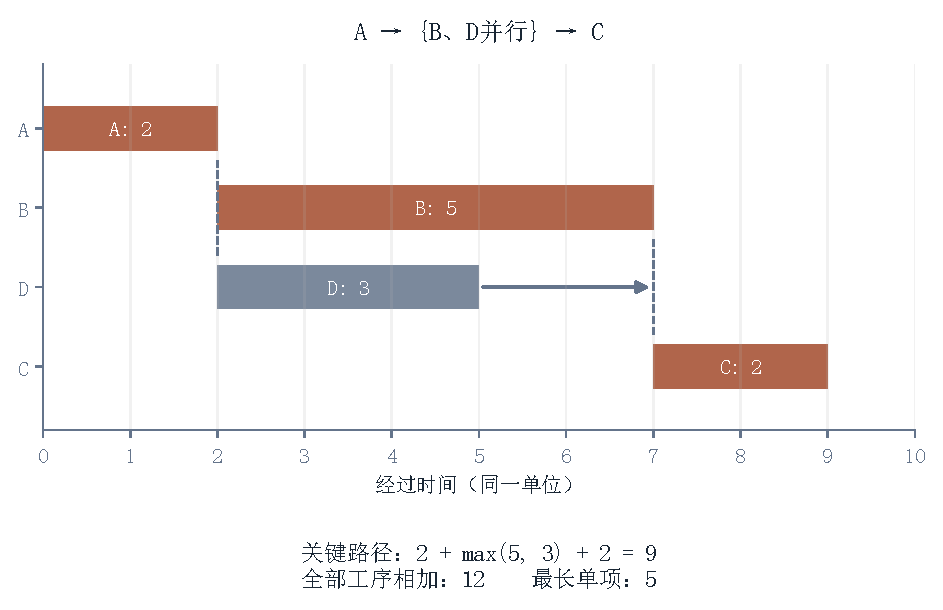
\includegraphics[width=\textwidth]{figures/critical-path.pdf}
\caption{A先执行，B与D随后并行，两项都完成后C才能开始。总历时为$2+\max(5,3)+2=9$，既不等于所有工序相加的12，也不等于最长单项的5。关键路径为A、B、C。}
\label{fig:mechanism-critical-path}
\end{figure}
\subsection{定位：大项与可改进项分别检查}

权重已知且刻度可比时，模型中较大的贡献项可以写为
\begin{equation}
c^\ast\in\operatorname*{arg\,max}_{c\in\{R,T,G\}}\alpha_c c,
\qquad(\alpha_R,\alpha_T,\alpha_G)=(\alpha,\beta,\gamma).
\label{eq:scale-dominant}
\end{equation}
未知权重时，不能仅凭哪个坐标的级数最大就宣布它主导总体黏滞。最大贡献项也未必是最值得优先改造的项，还要考察可行余量、成本、风险和相互作用。

在小幅、独立、边际成本近似固定的条件下，若压低一单位坐标$c$的成本为$\mu_c>0$，则
\begin{equation}
\frac{\alpha_c}{\mu_c}
\label{eq:scale-yield}
\end{equation}
比较的是每单位支出带来的模型内对数代价下降。它不是绝对净收益，也不处理跨维联动、有限预算、门槛与风险。有限项目仍须比较完整方案。

\begin{table}[ht]
\centering
\caption{从约束画像到改造选择}
\label{tab:scale-classes}
{\small
\begin{tabularx}{\textwidth}{@{}p{3.0cm}XX@{}}
\toprule
情形 & 要补的证据 & 可比较的行动\\
\midrule
主要约束可以低成本改善 & 改善幅度与全部成本 & 直接投入，并核验下游效果\\
改善会明显增加其他支出 & 联动幅度、承受者与风险 & 比较净效果及分配，重新设计接口\\
当前难改，但存在替代路径 & 替代任务、路线与结果标准 & 绕行、分阶段或缩小范围\\
多项约束同时偏高 & 全部可行路径与投入条件 & 重组方案，保留必要的等待与检验\\
\bottomrule
\end{tabularx}}
\end{table}

\subsection{示范一：低空服务的九个单元}

低空项目可以先拆成表\ref{tab:scale-lh}的九个单元。表中列的是应当查明的条件，具体等级要由选定机型、地区、运营范围与证据决定。

\begin{table}[ht]
\centering
\caption{低空服务：单元、约束与取证}
\label{tab:scale-lh}
{\small
\begin{tabularx}{\textwidth}{@{}p{3.2cm}XX@{}}
\toprule
单元 & 主要检查内容 & 应取得的证据\\
\midrule
电芯制造 & 配方、供给、良率与产能 & 产品规格、供应与生产记录\\
成组及热管理 & 系统质量、散热、故障隔离 & 包级测试与任务工况\\
机体及旋翼 & 材料、结构、制造与寿命 & 试验、工艺及维护依据\\
飞控与航电 & 功能、时延、失效与版本 & 需求、测试及审定记录\\
起降设施 & 场地、电力、接驳与备用 & 建设条件、接入与规划\\
运营维护 & 排班、备件、维修及恢复 & 运营设计与实测支持成本\\
适航审定 & 设计符合性与验证范围 & 对应辖区、型号与阶段文件\\
空域航路 & 运行边界、间隔与应急 & 适用规则及实际许可\\
服务接受 & 价格、噪声、可靠性与权益 & 对应人群的调查及运营反馈\\
\bottomrule
\end{tabularx}}
\end{table}

审定消耗人员、设备、试验与设施；协调和信任也需要物质载体与持续工作。不能因为输出是一份许可，就把资源记为零。公众接受需要定义人群和接受条件，不能先指定一个十年周期再据此预测落地。

把九个单元画成依赖图，区分可以并行的任务和必须等待的任务，再计算关键路径。电池改进可能同时改变载荷、备降裕量、经济性与审定证据；软件改进也可能减少试验负担。哪个环节控制投运时间，由项目的实际路径决定。

若许可仍在关键路径上，缩短不在该路径上的某道工序，可能不改变首次投运时间，却仍能降低费用或改善后续吞吐。把这几种结果分开，才能辨认改进究竟落在哪里。

\subsection{示范二：五类项目的比较入口}

\begin{table}[ht]
\centering
\caption{五类项目应分别核查的问题}
\label{tab:scale-five}
{\small
\begin{tabularx}{\textwidth}{@{}p{3.1cm}XX@{}}
\toprule
项目 & 资源与时间 & 依赖与确认\\
\midrule
大模型推理服务 & 现有容量、完整请求成本及扩容 & 输出触发什么下游行动\\
先进制程制造 & 设备、工序、良率与交付周期 & 哪些改动需要供应商与验证协同\\
低空服务 & 任务能耗、备份与设施条件 & 对应机型、空域和运营的证据\\
基因编辑治疗 & 递送、制造、观察与随访 & 细胞群体、临床终点与适用人群\\
水泥钢铁脱碳 & 工艺、能源、原料与更替周期 & 厂区、电力、运输、产品标准及需求\\
\bottomrule
\end{tabularx}}
\end{table}

同属一类项目，也可能采用不同技术路线和责任结构。基因编辑治疗不等于生殖系编辑，脱碳路线也不等于一种统一成熟工艺。先固定对象，再赋值与比较，行业名称只提供检索入口。

量表最终应当让争议落到具体证据上：哪个单元的什么条件改变了，依据是什么，哪些推论需要重算。能做到这一点，它就把总体判断变成了一份可复核的约束地图。

\section{三类响应模型与检验路线}

通量限制、需求吸收和适应性反馈，可以产生不同的响应形态。本节列出三种待检验模型，并给出相应数据口径。选取哪种形式，取决于具体任务的机制与观察；介质分类为选择提供线索。

数字服务的一种情形，是在需求与分发条件相对稳定时，实际使用率向平台趋近。平台可以受到注意力、预算、供给和产品适配等因素影响。单位生成成本与实际使用率需要分别测量，快速扩张的候选并不自动转成使用。

这条曲线的形状可以写成，

\begin{equation}
Y_{\text{比特}}(t)=Y_{\infty}\left(1-e^{-t/\tau_{\text{趋近}}}\right)
\end{equation}

$Y_{\text{比特}}$表示选定服务的使用率或有效处理率，$Y_\infty$为同口径的平台值，$\tau_{\text{趋近}}$为时间常数。式中初始值取零，早期近似线性上升，随后以指数衰减的偏差接近平台。平台位置和趋近速度须由数据估计，需求或供给变化以后可采用新的参数或形式。

固定设备、空间与能源供应，可能形成单位时间的实物产出上限。投入接近这套设施的能力时，增加投入的收益可以递减；新增设备、改变工艺或扩建网络，则可能改变上限。检验可以分别比较设计、制造、施工与维护的投入和产出，辨认AI究竟改善了哪些环节。

这条曲线的两个特征可以写成一组条件，

\begin{equation}
0\le Y_{\text{原子}}(I)\le \Phi_{\max},\qquad \frac{\partial^{2}Y_{\text{原子}}}{\partial I^{2}}\le0\quad(\text{饱和近似})
\end{equation}

$Y_{\text{原子}}$为实物产出率，$\Phi_{\max}$为给定设施条件下的最大可持续产出率，两者采用相同单位；$I$为统一口径的投入。第一项表达能力上界，第二项另加了饱和区间的凹性近似。阶跃扩产、学习效应或互补投入可能不满足凹性，需按观察选择其他形式。

能量比较也须固定任务。擦除一个比特、断开一个化学键和抬升一个宏观物体，分别选择了不同操作单位；它们的绝对值不能决定各产业的增长率。对一项完整任务，应核算所需操作次数、实际耗散、设备能力与有效产出，再比较设计改进和执行改进带来的收益。

适应性反馈可以改变剂量与效果的关系。一个可检验情形是：超过某个强度以后，平均收益趋于平台，而结果的离散程度继续增加。也可能观察到收益持续改善、作用下降或迟发响应。实验需要同时记录强度、作用时间、群体差异与后续观察，依据数据辨认具体反馈。

把这条检验路线写成判据就是，

\begin{equation}
\left.\frac{d\langle Y_{\text{生命}}\rangle}{dP}\right|_{P>P_{c}}\approx0,\qquad \left.\frac{d\,\mathrm{Var}(Y_{\text{生命}})}{dP}\right|_{P>P_{c}}>0
\end{equation}

$Y_{\text{生命}}$为选定结果指标，$P$为采用固定单位的干预强度，$P_c$为待估计的转折位置。均值与方差采用各自单位。式中的两个条件共同描述这一组平台与风险扩大的观察，其他反馈形态需要另外的函数。比较时须保留群体、观察时长和重复测量信息。

这三个示例分别选取时间、投入和干预强度作自变量，因而不能直接比较图上的斜率。要比较同一项智能技术在不同环节的效果，应先统一任务、投入与结果口径，再分别控制过程时间和环境条件。图形的差别来自机制假设，是否对应实际领域差异，仍由这种比较检验。

\begin{figure}[ht]
\centering
% >>>>>>>>>> figs/fig-scaling-laws.tex >>>>>>>>>>
% 图 A-1  三条演化曲线的形状与各自的横轴
% 这张图要读的不是三条曲线的具体高度，而是它们各自配了不同的横轴：
% (a) 时间／累计投入，(b) 投入，(c) 干预强度。正文那一节的结论正是
% 「把三条曲线放进同一个坐标系比较进步速度没有意义，因为横轴不同」，
% 所以三个横轴标签是图里最不能省的三处文字，其余一律压到最短。
% 纵轴一律不给数值刻度：(a)(b) 是相对产出，(c) 是收益与方差，
% 标上刻度会诱导读者去做这张示意图支持不了的横向比较。
% (c) 里方差线穿过平均收益线是刻意的——「超过阈值之后平均收益不再增加
% 而不确定性继续上升」在这个穿越上才看得见。
% 子图编号 (a)(b)(c) 一律放图下方。曲线用 plot[smooth]，因为这三条
% 本来就是连续可导的函数，与 fig-proof-abundance 里用折线的情形不同。
\begin{tikzpicture}[x=1cm, y=1cm, font=\small,
  ax/.style={-{Stealth[length=2.0mm]}, ink, line width=0.6pt}
]
\useasboundingbox (-0.30,3.90) rectangle (13.35,-0.62);

% ==================== (a) 比特：单调趋近 ====================
\node[font=\scriptsize, text=slate, anchor=center] at (2.15,3.62) {单调趋近};

\draw[slate!55, line width=0.9pt, dashed] (0.50,2.90) -- (3.80,2.90);
\node[font=\scriptsize, text=slate, anchor=west] at (3.86,2.90) {$Y_{\infty}$};

\draw[deepblue, line width=1.9pt] plot[smooth] coordinates {
  (0.50,0.60) (0.78,1.11) (1.06,1.50) (1.34,1.81) (1.62,2.05)
  (1.90,2.24) (2.18,2.39) (2.46,2.51) (2.74,2.60) (3.02,2.67)
  (3.30,2.73) (3.58,2.77) (3.80,2.79)
};

\draw[ax] (0.50,0.60) -- (4.02,0.60);
\draw[ax] (0.50,0.60) -- (0.50,3.42);
\node[font=\scriptsize, text=ink, anchor=north] at (2.15,0.42) {时间};
\node[font=\scriptsize, text=ink, rotate=90, anchor=south] at (0.34,2.00) {产出};

% ==================== (b) 原子：受通量约束 ====================
\node[font=\scriptsize, text=slate, anchor=center] at (6.60,3.62) {受通量约束};

\fill[rust!10] (4.95,3.10) rectangle (8.25,3.40);
\draw[rust!70, line width=0.9pt, dashed] (4.95,3.10) -- (8.25,3.10);
\node[font=\scriptsize, text=rust!85, anchor=north east] at (8.25,3.06) {$\Phi_{\max}$};

\draw[terra, line width=1.9pt] plot[smooth] coordinates {
  (4.95,0.60) (5.28,1.56) (5.61,1.82) (5.94,2.01) (6.27,2.16)
  (6.60,2.29) (6.93,2.40) (7.26,2.50) (7.59,2.59) (7.92,2.67)
  (8.25,2.75)
};

\draw[ax] (4.95,0.60) -- (8.47,0.60);
\draw[ax] (4.95,0.60) -- (4.95,3.42);
\node[font=\scriptsize, text=ink, anchor=north] at (6.60,0.42) {投入};
\node[font=\scriptsize, text=ink, rotate=90, anchor=south] at (4.79,2.00) {产出};

% ==================== (c) 生命：反馈型 ====================
\node[font=\scriptsize, text=slate, anchor=center] at (11.05,3.62) {反馈型};

\draw[rust!70, line width=0.9pt, dashed] (11.215,0.60) -- (11.215,3.10);
\node[font=\scriptsize, text=rust!85, anchor=east] at (11.11,1.78) {$P_{c}$};

% 平均收益：升到阈值后转平
\draw[forest, line width=1.9pt] plot[smooth] coordinates {
  (9.40,0.60) (9.73,1.03) (10.06,1.42) (10.39,1.76) (10.72,2.06)
  (11.05,2.33) (11.22,2.45) (11.60,2.45) (12.15,2.45) (12.70,2.45)
};
% 不确定性：阈值前基本不动，阈值后迅速上升
\draw[rust, line width=1.9pt] plot[smooth] coordinates {
  (9.40,1.05) (9.95,1.06) (10.50,1.09) (11.05,1.14) (11.22,1.18)
  (11.60,1.55) (11.95,2.05) (12.30,2.58) (12.70,3.08)
};

\draw[forest, line width=1.5pt] (9.55,3.22) -- (9.98,3.22);
\node[font=\scriptsize, text=forest, anchor=west] at (10.05,3.22) {平均收益};
\draw[rust, line width=1.5pt] (9.55,2.92) -- (9.98,2.92);
\node[font=\scriptsize, text=rust, anchor=west] at (10.05,2.92) {不确定性};

\draw[ax] (9.40,0.60) -- (12.92,0.60);
\draw[ax] (9.40,0.60) -- (9.40,3.42);
\node[font=\scriptsize, text=ink, anchor=north] at (11.05,0.42) {干预强度};
\node[font=\scriptsize, text=ink, rotate=90, anchor=south] at (9.24,2.00) {各自归一化结果};

% ==================== 子图编号，一律放下面 ====================
\node[font=\small, text=ink] at (2.15,-0.28) {(a)};
\node[font=\small, text=ink] at (6.60,-0.28) {(b)};
\node[font=\small, text=ink] at (11.05,-0.28) {(c)};
\end{tikzpicture}

% <<<<<<<<<< figs/fig-scaling-laws.tex <<<<<<<<<<

\caption{三个响应模型的概念示意。(a) 使用率随时间趋近平台，(b) 给定设施内产出率随投入饱和，(c) 平均收益趋平而结果方差增加。各纵轴独立归一化，尤其(c)的均值与方差不共用物理单位；线条高度及交点不供跨指标比较。}
\label{fig:scaling-laws}
\end{figure}

把三条曲线并排列出，差别落在四列上。

\begin{table}[ht]
\centering
\caption{三条演化曲线的自变量、判据与可用的检验数据}
\label{tab:scaling-laws}
{\small
\begin{tabularx}{\textwidth}{@{}>{\RaggedRight\arraybackslash}p{2.45cm} >{\RaggedRight\arraybackslash}p{1.9cm} >{\RaggedRight\arraybackslash}p{4.0cm} >{\RaggedRight\arraybackslash}X@{}}
\toprule
曲线 & 自变量 & 判据 & 可用的检验数据 \\
\midrule
比特：单调趋近 & 时间 & $Y_{\text{比特}}\to Y_{\infty}$，平台与时间常数由任务数据估计 & 文本、图像、代码生成的单位成本时间序列，以及这些产出的实际使用率，而非产出量 \\
原子：受通量约束 & 投入 $I$ & $Y_{\text{原子}}\le\Phi_{\max}$，饱和区间另检验$\partial^{2}Y_{\text{原子}}/\partial I^{2}\le0$ & 建筑业劳动生产率、采矿与冶炼的能耗强度、半导体制造的单位投资；同一项目在设计阶段与施工阶段的工期压缩比 \\
生命：反馈型 & 干预强度 $P$ & 在 $P>P_{c}$ 上 $d\langle Y_{\text{生命}}\rangle/dP\approx0$，且 $d\,\mathrm{Var}(Y_{\text{生命}})/dP>0$ & 药物剂量、疗效与副作用的配对测量；编辑强度与脱靶率的配对测量 \\
\bottomrule
\end{tabularx}}
\end{table}

表 \ref{tab:scaling-laws} 的四列里，只有第三列可以脱离本书的术语使用：判据一栏写的是可以直接从数据里取到的条件，不要求读者先接受 $\eta$、$De$ 或三类介质的分类。这是这张表与全书其余部分的关系：分类是本书提出的，检验不是。三条曲线的判据彼此独立，任何一条被观测否定，对应的那条曲线就要改写，另外两条不受影响，因为它们各自的自变量与判据都是分开写出来的。

同一技术通常穿过多个环节，结果还受到相互作用影响。总产出未必是三条曲线的线性叠加。可行的起点，是选择边界稳定的任务，分别记录设计、执行、验证与维护的时间和成本，再用对照、分阶段部署或可比较项目检查机制。整体效果的解释，要在这些环节关系得到支持以后推进。

\section{认识论边界}

框架的评价分成三层：约束分类能否帮助辨认机制，数量模型能否解释并区分观察结果，规范主张能否给出公开理由。三者采用各自的证据，修订也应回到相应层面。

第一，分类框架组织问题，经过标定的数量模型才承担具体预测。预测需要固定任务、变量、基准与参数，并检验样本外表现。仅凭区域名称或未标定公式，可以列出要检查的约束，不能确定某项技术的部署年份、增长速度或临界点。

第二，物理形式进入社会技术分析，需要明确机制对应。借用剪切增稠形式时，要指出干预速率怎样引发代偿或结构变化；借用德博拉数时，要测量响应与输入的时间尺度。结构对应得到支持，模型才有解释力；对应不成立，就要更换形式。词汇相似不能代替这种检查。

第三，分类与函数形式分别接受检验。对数线性形式要与交互、阈值和其他候选形式比较，并在独立数据上检查误差；介质分类要检验是否增加了机制解释与样本外区分能力。若模型依赖反复改动变量含义才能拟合，就要重审定义。不同介质出现相似曲线，要求回到机制和任务尺度判断，曲线相似本身既不证实也不推翻整个框架。

第四，约束分析说明哪些条件影响转移代价，价值论证说明为什么某些结果、权利和责任值得被保护。本书主张让受影响者能够参与、让判断保留证据、让决定接受追责。支持这些主张，需要公开伦理理由、程序与分配安排；物理下限不替这些理由作决定。

第七章据此提出选择、分配与承担黏滞的实践主张。应用到具体决定时，先查清可行路径与成本分布，再比较结果涉及的利益和权利，最后确定授权与责任。数据支持可行性判断，规范理由支持取舍，实施记录让判断继续接受检验。

% <<<<<<<<<< parts/book-ch07.tex <<<<<<<<<<


%% ===================== 本章参考文献 =====================
\printbibliography[heading=subbibliography,title=参考文献]

\end{document}
